\documentclass[final]{beamer}

\usepackage[T1]{fontenc}
\usepackage{lmodern}
\usepackage[size=A0]{beamerposter}
\usetheme{gemini}
\usecolortheme{mit}
\usepackage{graphicx}
\usepackage{booktabs}
\usepackage{tikz}
\usepackage{pgfplots}
\usepackage{bm}
\usepackage[binary-units=true,per-mode=symbol]{siunitx}
\DeclareMathOperator{\erf}{erf}
\usefonttheme[onlymath]{serif}

% If you have N columns, choose \sepwidth and \colwidth such that
% (N+1)*\sepwidth + N*\colwidth = \paperwidth
\newlength{\sepwidth}
\newlength{\colwidth}
\setlength{\sepwidth}{0.025\paperwidth}
\setlength{\colwidth}{0.3\paperwidth}

\newcommand{\separatorcolumn}{\begin{column}{\sepwidth}\end{column}}

\title{Accurate and Robust PMT Waveform Analysis}

\author{E.~Bao\inst{1} \and Y.~Wu\inst{2} \and B.~D.~Xu\inst{2} \and D.~C.~Xu\inst{2} \and Y.~Xu\inst{3} \and G.~Zhang\inst{4}}

\institute[shortinst]{\inst{a} National Institute of Informatics \samelineand \inst{b} Tsinghua University \samelineand \inst{c} Forschungszentrum Jülich \samelineand \inst{d} Southwestern University of Finance and Economics}

% use this to include logos on the left and/or right side of the header:
% \logoright{\includegraphics[height=7cm]{logo1.pdf}}
% \logoleft{\includegraphics[height=7cm]{logo2.pdf}}

\begin{document}

\begin{frame}[t]
\begin{columns}[t]
\separatorcolumn

\begin{column}{\colwidth}

  \begin{block}{Motivation}

    \begin{columns}
    \column{0.5\textwidth}
    \begin{figure}
        \centering
        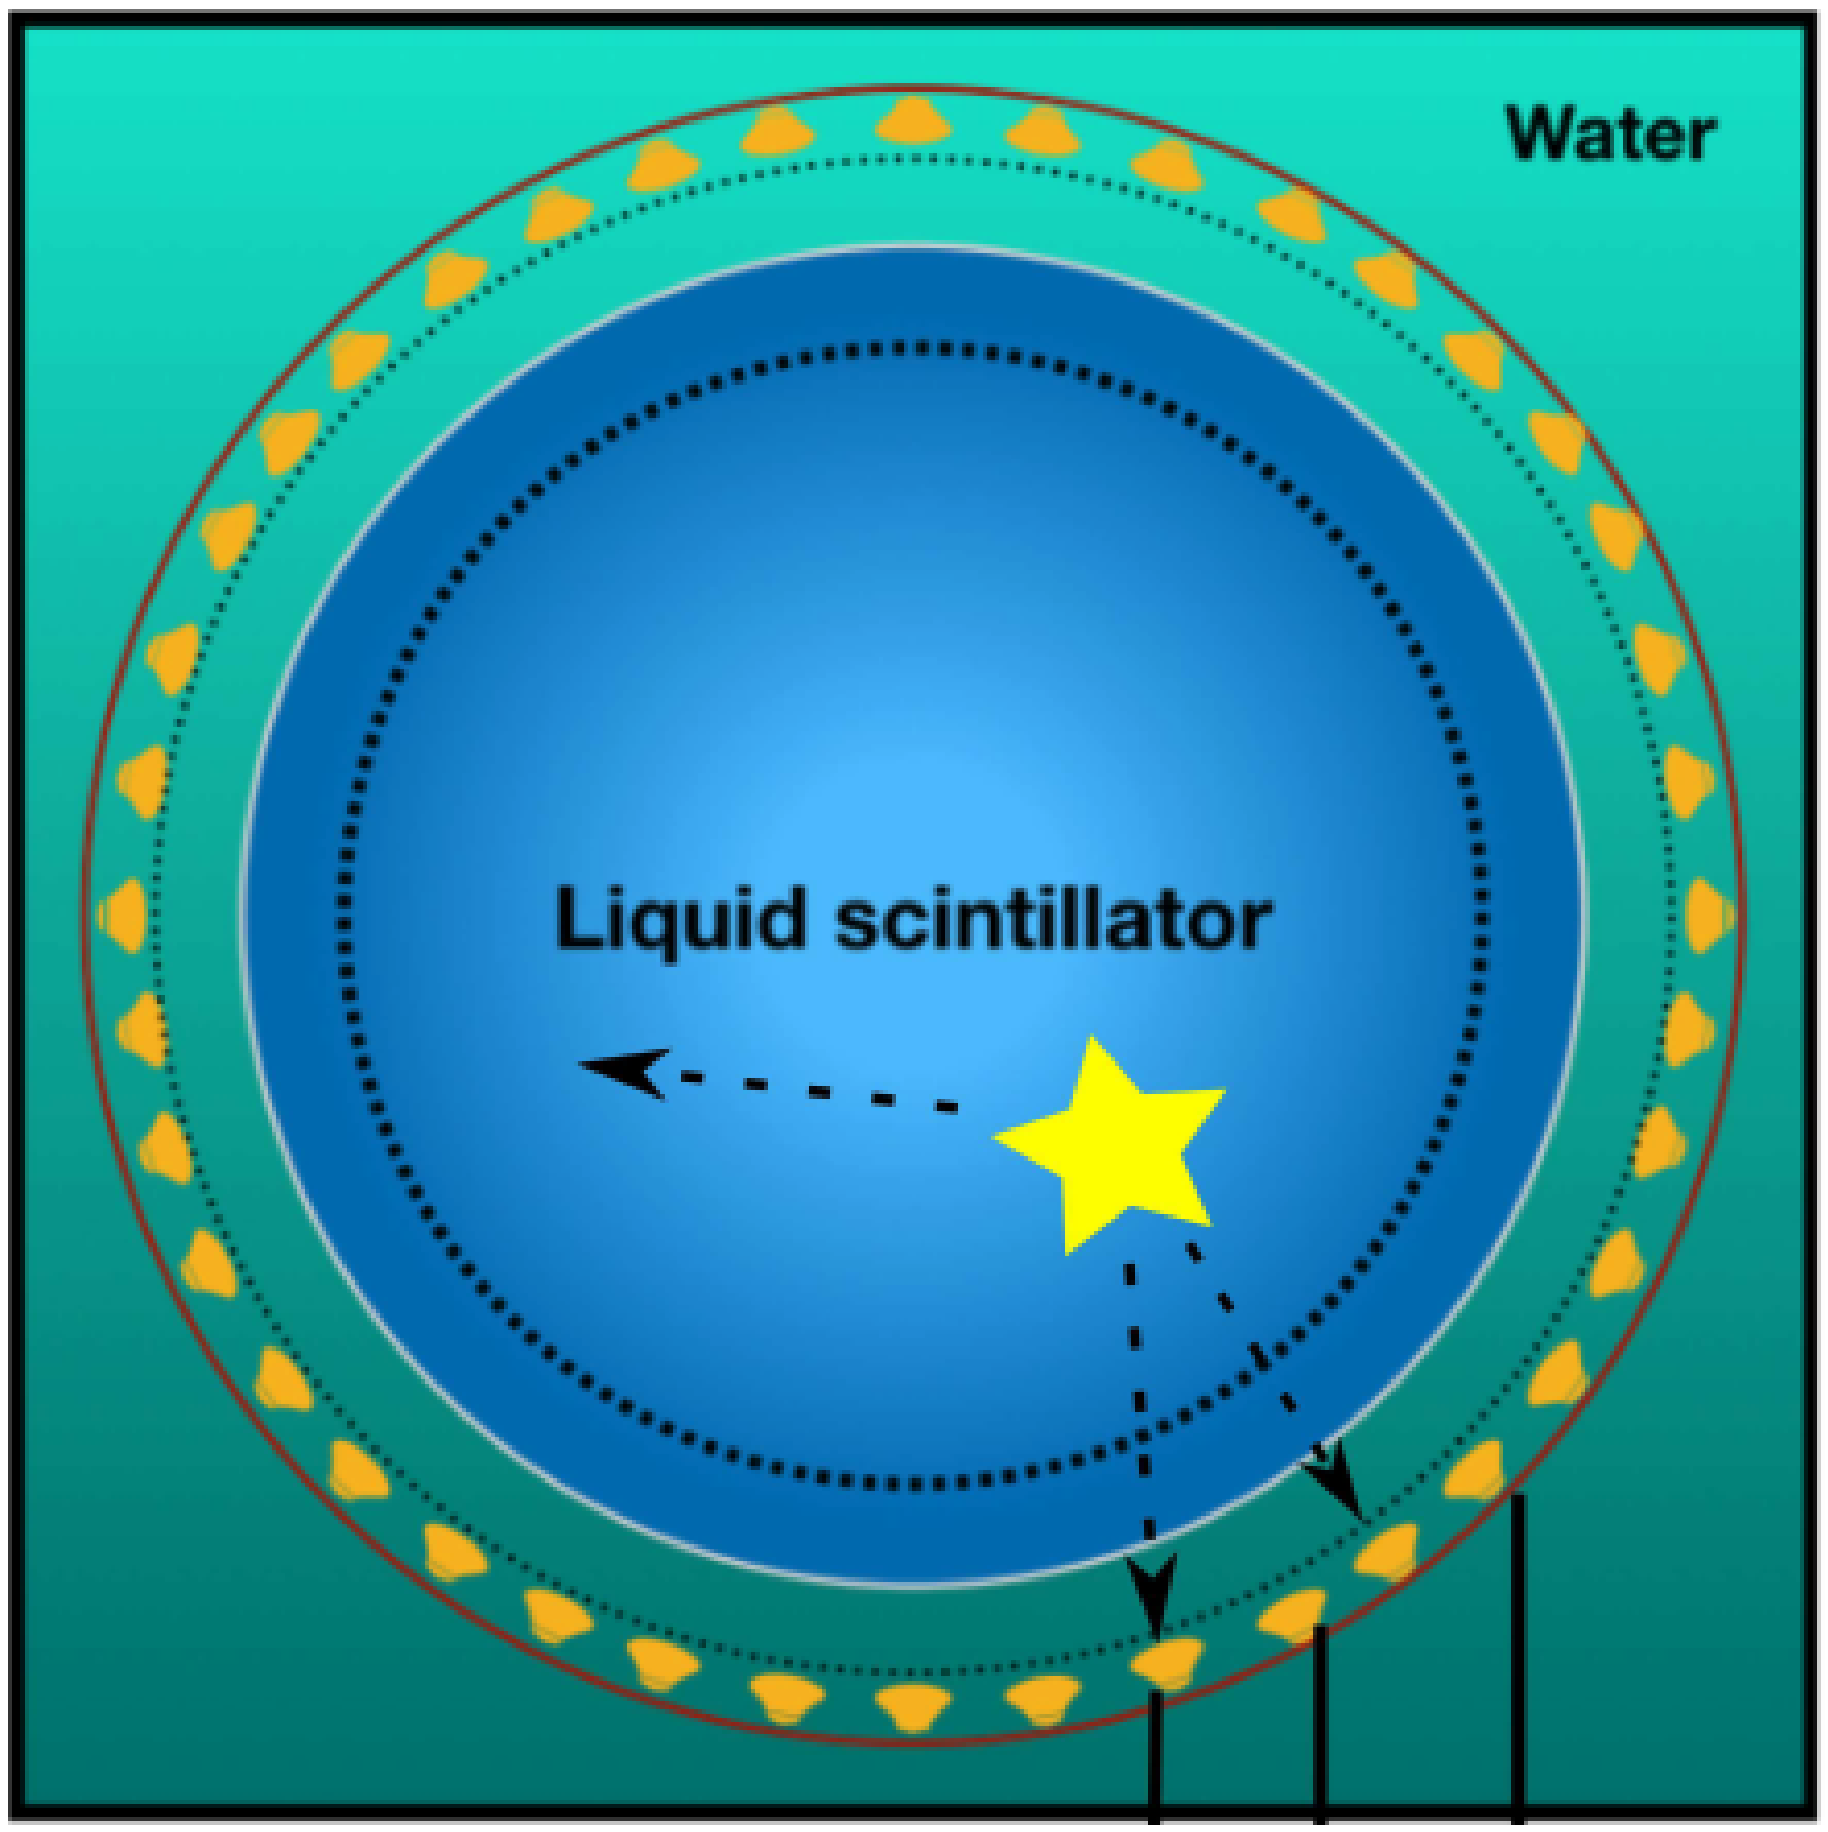
\includegraphics[width=0.4\linewidth]{img/event.png}
        \caption{An Event in Detector}
    \end{figure}
    \column{0.5\textwidth}
    \begin{figure}
        \centering
        \resizebox{0.9\textwidth}{!}{%% Creator: Matplotlib, PGF backend
%%
%% To include the figure in your LaTeX document, write
%%   \input{<filename>.pgf}
%%
%% Make sure the required packages are loaded in your preamble
%%   \usepackage{pgf}
%%
%% and, on pdftex
%%   \usepackage[utf8]{inputenc}\DeclareUnicodeCharacter{2212}{-}
%%
%% or, on luatex and xetex
%%   \usepackage{unicode-math}
%%
%% Figures using additional raster images can only be included by \input if
%% they are in the same directory as the main LaTeX file. For loading figures
%% from other directories you can use the `import` package
%%   \usepackage{import}
%%
%% and then include the figures with
%%   \import{<path to file>}{<filename>.pgf}
%%
%% Matplotlib used the following preamble
%%   \usepackage[detect-all,locale=DE]{siunitx}
%%
\begingroup%
\makeatletter%
\begin{pgfpicture}%
\pgfpathrectangle{\pgfpointorigin}{\pgfqpoint{12.000000in}{6.000000in}}%
\pgfusepath{use as bounding box, clip}%
\begin{pgfscope}%
\pgfsetbuttcap%
\pgfsetmiterjoin%
\definecolor{currentfill}{rgb}{1.000000,1.000000,1.000000}%
\pgfsetfillcolor{currentfill}%
\pgfsetlinewidth{0.000000pt}%
\definecolor{currentstroke}{rgb}{1.000000,1.000000,1.000000}%
\pgfsetstrokecolor{currentstroke}%
\pgfsetdash{}{0pt}%
\pgfpathmoveto{\pgfqpoint{0.000000in}{0.000000in}}%
\pgfpathlineto{\pgfqpoint{12.000000in}{0.000000in}}%
\pgfpathlineto{\pgfqpoint{12.000000in}{6.000000in}}%
\pgfpathlineto{\pgfqpoint{0.000000in}{6.000000in}}%
\pgfpathclose%
\pgfusepath{fill}%
\end{pgfscope}%
\begin{pgfscope}%
\pgfsetbuttcap%
\pgfsetmiterjoin%
\definecolor{currentfill}{rgb}{1.000000,1.000000,1.000000}%
\pgfsetfillcolor{currentfill}%
\pgfsetlinewidth{0.000000pt}%
\definecolor{currentstroke}{rgb}{0.000000,0.000000,0.000000}%
\pgfsetstrokecolor{currentstroke}%
\pgfsetstrokeopacity{0.000000}%
\pgfsetdash{}{0pt}%
\pgfpathmoveto{\pgfqpoint{1.800000in}{0.900000in}}%
\pgfpathlineto{\pgfqpoint{10.200000in}{0.900000in}}%
\pgfpathlineto{\pgfqpoint{10.200000in}{5.700000in}}%
\pgfpathlineto{\pgfqpoint{1.800000in}{5.700000in}}%
\pgfpathclose%
\pgfusepath{fill}%
\end{pgfscope}%
\begin{pgfscope}%
\pgfsetbuttcap%
\pgfsetroundjoin%
\definecolor{currentfill}{rgb}{0.000000,0.000000,0.000000}%
\pgfsetfillcolor{currentfill}%
\pgfsetlinewidth{0.803000pt}%
\definecolor{currentstroke}{rgb}{0.000000,0.000000,0.000000}%
\pgfsetstrokecolor{currentstroke}%
\pgfsetdash{}{0pt}%
\pgfsys@defobject{currentmarker}{\pgfqpoint{0.000000in}{-0.048611in}}{\pgfqpoint{0.000000in}{0.000000in}}{%
\pgfpathmoveto{\pgfqpoint{0.000000in}{0.000000in}}%
\pgfpathlineto{\pgfqpoint{0.000000in}{-0.048611in}}%
\pgfusepath{stroke,fill}%
}%
\begin{pgfscope}%
\pgfsys@transformshift{1.800000in}{0.900000in}%
\pgfsys@useobject{currentmarker}{}%
\end{pgfscope}%
\end{pgfscope}%
\begin{pgfscope}%
\definecolor{textcolor}{rgb}{0.000000,0.000000,0.000000}%
\pgfsetstrokecolor{textcolor}%
\pgfsetfillcolor{textcolor}%
\pgftext[x=1.800000in,y=0.802778in,,top]{\color{textcolor}\sffamily\fontsize{20.000000}{24.000000}\selectfont \(\displaystyle {0}\)}%
\end{pgfscope}%
\begin{pgfscope}%
\pgfsetbuttcap%
\pgfsetroundjoin%
\definecolor{currentfill}{rgb}{0.000000,0.000000,0.000000}%
\pgfsetfillcolor{currentfill}%
\pgfsetlinewidth{0.803000pt}%
\definecolor{currentstroke}{rgb}{0.000000,0.000000,0.000000}%
\pgfsetstrokecolor{currentstroke}%
\pgfsetdash{}{0pt}%
\pgfsys@defobject{currentmarker}{\pgfqpoint{0.000000in}{-0.048611in}}{\pgfqpoint{0.000000in}{0.000000in}}{%
\pgfpathmoveto{\pgfqpoint{0.000000in}{0.000000in}}%
\pgfpathlineto{\pgfqpoint{0.000000in}{-0.048611in}}%
\pgfusepath{stroke,fill}%
}%
\begin{pgfscope}%
\pgfsys@transformshift{3.432653in}{0.900000in}%
\pgfsys@useobject{currentmarker}{}%
\end{pgfscope}%
\end{pgfscope}%
\begin{pgfscope}%
\definecolor{textcolor}{rgb}{0.000000,0.000000,0.000000}%
\pgfsetstrokecolor{textcolor}%
\pgfsetfillcolor{textcolor}%
\pgftext[x=3.432653in,y=0.802778in,,top]{\color{textcolor}\sffamily\fontsize{20.000000}{24.000000}\selectfont \(\displaystyle {200}\)}%
\end{pgfscope}%
\begin{pgfscope}%
\pgfsetbuttcap%
\pgfsetroundjoin%
\definecolor{currentfill}{rgb}{0.000000,0.000000,0.000000}%
\pgfsetfillcolor{currentfill}%
\pgfsetlinewidth{0.803000pt}%
\definecolor{currentstroke}{rgb}{0.000000,0.000000,0.000000}%
\pgfsetstrokecolor{currentstroke}%
\pgfsetdash{}{0pt}%
\pgfsys@defobject{currentmarker}{\pgfqpoint{0.000000in}{-0.048611in}}{\pgfqpoint{0.000000in}{0.000000in}}{%
\pgfpathmoveto{\pgfqpoint{0.000000in}{0.000000in}}%
\pgfpathlineto{\pgfqpoint{0.000000in}{-0.048611in}}%
\pgfusepath{stroke,fill}%
}%
\begin{pgfscope}%
\pgfsys@transformshift{5.065306in}{0.900000in}%
\pgfsys@useobject{currentmarker}{}%
\end{pgfscope}%
\end{pgfscope}%
\begin{pgfscope}%
\definecolor{textcolor}{rgb}{0.000000,0.000000,0.000000}%
\pgfsetstrokecolor{textcolor}%
\pgfsetfillcolor{textcolor}%
\pgftext[x=5.065306in,y=0.802778in,,top]{\color{textcolor}\sffamily\fontsize{20.000000}{24.000000}\selectfont \(\displaystyle {400}\)}%
\end{pgfscope}%
\begin{pgfscope}%
\pgfsetbuttcap%
\pgfsetroundjoin%
\definecolor{currentfill}{rgb}{0.000000,0.000000,0.000000}%
\pgfsetfillcolor{currentfill}%
\pgfsetlinewidth{0.803000pt}%
\definecolor{currentstroke}{rgb}{0.000000,0.000000,0.000000}%
\pgfsetstrokecolor{currentstroke}%
\pgfsetdash{}{0pt}%
\pgfsys@defobject{currentmarker}{\pgfqpoint{0.000000in}{-0.048611in}}{\pgfqpoint{0.000000in}{0.000000in}}{%
\pgfpathmoveto{\pgfqpoint{0.000000in}{0.000000in}}%
\pgfpathlineto{\pgfqpoint{0.000000in}{-0.048611in}}%
\pgfusepath{stroke,fill}%
}%
\begin{pgfscope}%
\pgfsys@transformshift{6.697959in}{0.900000in}%
\pgfsys@useobject{currentmarker}{}%
\end{pgfscope}%
\end{pgfscope}%
\begin{pgfscope}%
\definecolor{textcolor}{rgb}{0.000000,0.000000,0.000000}%
\pgfsetstrokecolor{textcolor}%
\pgfsetfillcolor{textcolor}%
\pgftext[x=6.697959in,y=0.802778in,,top]{\color{textcolor}\sffamily\fontsize{20.000000}{24.000000}\selectfont \(\displaystyle {600}\)}%
\end{pgfscope}%
\begin{pgfscope}%
\pgfsetbuttcap%
\pgfsetroundjoin%
\definecolor{currentfill}{rgb}{0.000000,0.000000,0.000000}%
\pgfsetfillcolor{currentfill}%
\pgfsetlinewidth{0.803000pt}%
\definecolor{currentstroke}{rgb}{0.000000,0.000000,0.000000}%
\pgfsetstrokecolor{currentstroke}%
\pgfsetdash{}{0pt}%
\pgfsys@defobject{currentmarker}{\pgfqpoint{0.000000in}{-0.048611in}}{\pgfqpoint{0.000000in}{0.000000in}}{%
\pgfpathmoveto{\pgfqpoint{0.000000in}{0.000000in}}%
\pgfpathlineto{\pgfqpoint{0.000000in}{-0.048611in}}%
\pgfusepath{stroke,fill}%
}%
\begin{pgfscope}%
\pgfsys@transformshift{8.330612in}{0.900000in}%
\pgfsys@useobject{currentmarker}{}%
\end{pgfscope}%
\end{pgfscope}%
\begin{pgfscope}%
\definecolor{textcolor}{rgb}{0.000000,0.000000,0.000000}%
\pgfsetstrokecolor{textcolor}%
\pgfsetfillcolor{textcolor}%
\pgftext[x=8.330612in,y=0.802778in,,top]{\color{textcolor}\sffamily\fontsize{20.000000}{24.000000}\selectfont \(\displaystyle {800}\)}%
\end{pgfscope}%
\begin{pgfscope}%
\pgfsetbuttcap%
\pgfsetroundjoin%
\definecolor{currentfill}{rgb}{0.000000,0.000000,0.000000}%
\pgfsetfillcolor{currentfill}%
\pgfsetlinewidth{0.803000pt}%
\definecolor{currentstroke}{rgb}{0.000000,0.000000,0.000000}%
\pgfsetstrokecolor{currentstroke}%
\pgfsetdash{}{0pt}%
\pgfsys@defobject{currentmarker}{\pgfqpoint{0.000000in}{-0.048611in}}{\pgfqpoint{0.000000in}{0.000000in}}{%
\pgfpathmoveto{\pgfqpoint{0.000000in}{0.000000in}}%
\pgfpathlineto{\pgfqpoint{0.000000in}{-0.048611in}}%
\pgfusepath{stroke,fill}%
}%
\begin{pgfscope}%
\pgfsys@transformshift{9.963265in}{0.900000in}%
\pgfsys@useobject{currentmarker}{}%
\end{pgfscope}%
\end{pgfscope}%
\begin{pgfscope}%
\definecolor{textcolor}{rgb}{0.000000,0.000000,0.000000}%
\pgfsetstrokecolor{textcolor}%
\pgfsetfillcolor{textcolor}%
\pgftext[x=9.963265in,y=0.802778in,,top]{\color{textcolor}\sffamily\fontsize{20.000000}{24.000000}\selectfont \(\displaystyle {1000}\)}%
\end{pgfscope}%
\begin{pgfscope}%
\definecolor{textcolor}{rgb}{0.000000,0.000000,0.000000}%
\pgfsetstrokecolor{textcolor}%
\pgfsetfillcolor{textcolor}%
\pgftext[x=6.000000in,y=0.491155in,,top]{\color{textcolor}\sffamily\fontsize{20.000000}{24.000000}\selectfont \(\displaystyle \mathrm{t}/\si{ns}\)}%
\end{pgfscope}%
\begin{pgfscope}%
\pgfsetbuttcap%
\pgfsetroundjoin%
\definecolor{currentfill}{rgb}{0.000000,0.000000,0.000000}%
\pgfsetfillcolor{currentfill}%
\pgfsetlinewidth{0.803000pt}%
\definecolor{currentstroke}{rgb}{0.000000,0.000000,0.000000}%
\pgfsetstrokecolor{currentstroke}%
\pgfsetdash{}{0pt}%
\pgfsys@defobject{currentmarker}{\pgfqpoint{-0.048611in}{0.000000in}}{\pgfqpoint{-0.000000in}{0.000000in}}{%
\pgfpathmoveto{\pgfqpoint{-0.000000in}{0.000000in}}%
\pgfpathlineto{\pgfqpoint{-0.048611in}{0.000000in}}%
\pgfusepath{stroke,fill}%
}%
\begin{pgfscope}%
\pgfsys@transformshift{1.800000in}{1.109935in}%
\pgfsys@useobject{currentmarker}{}%
\end{pgfscope}%
\end{pgfscope}%
\begin{pgfscope}%
\definecolor{textcolor}{rgb}{0.000000,0.000000,0.000000}%
\pgfsetstrokecolor{textcolor}%
\pgfsetfillcolor{textcolor}%
\pgftext[x=1.306456in, y=1.009915in, left, base]{\color{textcolor}\sffamily\fontsize{20.000000}{24.000000}\selectfont \(\displaystyle {880}\)}%
\end{pgfscope}%
\begin{pgfscope}%
\pgfsetbuttcap%
\pgfsetroundjoin%
\definecolor{currentfill}{rgb}{0.000000,0.000000,0.000000}%
\pgfsetfillcolor{currentfill}%
\pgfsetlinewidth{0.803000pt}%
\definecolor{currentstroke}{rgb}{0.000000,0.000000,0.000000}%
\pgfsetstrokecolor{currentstroke}%
\pgfsetdash{}{0pt}%
\pgfsys@defobject{currentmarker}{\pgfqpoint{-0.048611in}{0.000000in}}{\pgfqpoint{-0.000000in}{0.000000in}}{%
\pgfpathmoveto{\pgfqpoint{-0.000000in}{0.000000in}}%
\pgfpathlineto{\pgfqpoint{-0.048611in}{0.000000in}}%
\pgfusepath{stroke,fill}%
}%
\begin{pgfscope}%
\pgfsys@transformshift{1.800000in}{2.054008in}%
\pgfsys@useobject{currentmarker}{}%
\end{pgfscope}%
\end{pgfscope}%
\begin{pgfscope}%
\definecolor{textcolor}{rgb}{0.000000,0.000000,0.000000}%
\pgfsetstrokecolor{textcolor}%
\pgfsetfillcolor{textcolor}%
\pgftext[x=1.306456in, y=1.953989in, left, base]{\color{textcolor}\sffamily\fontsize{20.000000}{24.000000}\selectfont \(\displaystyle {885}\)}%
\end{pgfscope}%
\begin{pgfscope}%
\pgfsetbuttcap%
\pgfsetroundjoin%
\definecolor{currentfill}{rgb}{0.000000,0.000000,0.000000}%
\pgfsetfillcolor{currentfill}%
\pgfsetlinewidth{0.803000pt}%
\definecolor{currentstroke}{rgb}{0.000000,0.000000,0.000000}%
\pgfsetstrokecolor{currentstroke}%
\pgfsetdash{}{0pt}%
\pgfsys@defobject{currentmarker}{\pgfqpoint{-0.048611in}{0.000000in}}{\pgfqpoint{-0.000000in}{0.000000in}}{%
\pgfpathmoveto{\pgfqpoint{-0.000000in}{0.000000in}}%
\pgfpathlineto{\pgfqpoint{-0.048611in}{0.000000in}}%
\pgfusepath{stroke,fill}%
}%
\begin{pgfscope}%
\pgfsys@transformshift{1.800000in}{2.998081in}%
\pgfsys@useobject{currentmarker}{}%
\end{pgfscope}%
\end{pgfscope}%
\begin{pgfscope}%
\definecolor{textcolor}{rgb}{0.000000,0.000000,0.000000}%
\pgfsetstrokecolor{textcolor}%
\pgfsetfillcolor{textcolor}%
\pgftext[x=1.306456in, y=2.898062in, left, base]{\color{textcolor}\sffamily\fontsize{20.000000}{24.000000}\selectfont \(\displaystyle {890}\)}%
\end{pgfscope}%
\begin{pgfscope}%
\pgfsetbuttcap%
\pgfsetroundjoin%
\definecolor{currentfill}{rgb}{0.000000,0.000000,0.000000}%
\pgfsetfillcolor{currentfill}%
\pgfsetlinewidth{0.803000pt}%
\definecolor{currentstroke}{rgb}{0.000000,0.000000,0.000000}%
\pgfsetstrokecolor{currentstroke}%
\pgfsetdash{}{0pt}%
\pgfsys@defobject{currentmarker}{\pgfqpoint{-0.048611in}{0.000000in}}{\pgfqpoint{-0.000000in}{0.000000in}}{%
\pgfpathmoveto{\pgfqpoint{-0.000000in}{0.000000in}}%
\pgfpathlineto{\pgfqpoint{-0.048611in}{0.000000in}}%
\pgfusepath{stroke,fill}%
}%
\begin{pgfscope}%
\pgfsys@transformshift{1.800000in}{3.942154in}%
\pgfsys@useobject{currentmarker}{}%
\end{pgfscope}%
\end{pgfscope}%
\begin{pgfscope}%
\definecolor{textcolor}{rgb}{0.000000,0.000000,0.000000}%
\pgfsetstrokecolor{textcolor}%
\pgfsetfillcolor{textcolor}%
\pgftext[x=1.306456in, y=3.842135in, left, base]{\color{textcolor}\sffamily\fontsize{20.000000}{24.000000}\selectfont \(\displaystyle {895}\)}%
\end{pgfscope}%
\begin{pgfscope}%
\pgfsetbuttcap%
\pgfsetroundjoin%
\definecolor{currentfill}{rgb}{0.000000,0.000000,0.000000}%
\pgfsetfillcolor{currentfill}%
\pgfsetlinewidth{0.803000pt}%
\definecolor{currentstroke}{rgb}{0.000000,0.000000,0.000000}%
\pgfsetstrokecolor{currentstroke}%
\pgfsetdash{}{0pt}%
\pgfsys@defobject{currentmarker}{\pgfqpoint{-0.048611in}{0.000000in}}{\pgfqpoint{-0.000000in}{0.000000in}}{%
\pgfpathmoveto{\pgfqpoint{-0.000000in}{0.000000in}}%
\pgfpathlineto{\pgfqpoint{-0.048611in}{0.000000in}}%
\pgfusepath{stroke,fill}%
}%
\begin{pgfscope}%
\pgfsys@transformshift{1.800000in}{4.886228in}%
\pgfsys@useobject{currentmarker}{}%
\end{pgfscope}%
\end{pgfscope}%
\begin{pgfscope}%
\definecolor{textcolor}{rgb}{0.000000,0.000000,0.000000}%
\pgfsetstrokecolor{textcolor}%
\pgfsetfillcolor{textcolor}%
\pgftext[x=1.306456in, y=4.786208in, left, base]{\color{textcolor}\sffamily\fontsize{20.000000}{24.000000}\selectfont \(\displaystyle {900}\)}%
\end{pgfscope}%
\begin{pgfscope}%
\definecolor{textcolor}{rgb}{0.000000,0.000000,0.000000}%
\pgfsetstrokecolor{textcolor}%
\pgfsetfillcolor{textcolor}%
\pgftext[x=1.250900in,y=3.300000in,,bottom,rotate=90.000000]{\color{textcolor}\sffamily\fontsize{20.000000}{24.000000}\selectfont \(\displaystyle \mathrm{Voltage}/\si{mV}\)}%
\end{pgfscope}%
\begin{pgfscope}%
\pgfpathrectangle{\pgfqpoint{1.800000in}{0.900000in}}{\pgfqpoint{8.400000in}{4.800000in}}%
\pgfusepath{clip}%
\pgfsetrectcap%
\pgfsetroundjoin%
\pgfsetlinewidth{2.007500pt}%
\definecolor{currentstroke}{rgb}{0.121569,0.466667,0.705882}%
\pgfsetstrokecolor{currentstroke}%
\pgfsetdash{}{0pt}%
\pgfpathmoveto{\pgfqpoint{1.800000in}{4.676904in}}%
\pgfpathlineto{\pgfqpoint{1.808163in}{4.980346in}}%
\pgfpathlineto{\pgfqpoint{1.816327in}{4.954313in}}%
\pgfpathlineto{\pgfqpoint{1.824490in}{4.735669in}}%
\pgfpathlineto{\pgfqpoint{1.832653in}{4.846744in}}%
\pgfpathlineto{\pgfqpoint{1.840816in}{5.197049in}}%
\pgfpathlineto{\pgfqpoint{1.848980in}{4.897706in}}%
\pgfpathlineto{\pgfqpoint{1.857143in}{5.008569in}}%
\pgfpathlineto{\pgfqpoint{1.865306in}{4.809978in}}%
\pgfpathlineto{\pgfqpoint{1.873469in}{5.106843in}}%
\pgfpathlineto{\pgfqpoint{1.881633in}{4.814257in}}%
\pgfpathlineto{\pgfqpoint{1.889796in}{5.041644in}}%
\pgfpathlineto{\pgfqpoint{1.897959in}{4.992010in}}%
\pgfpathlineto{\pgfqpoint{1.906122in}{5.104570in}}%
\pgfpathlineto{\pgfqpoint{1.914286in}{5.178215in}}%
\pgfpathlineto{\pgfqpoint{1.922449in}{4.892378in}}%
\pgfpathlineto{\pgfqpoint{1.930612in}{4.565990in}}%
\pgfpathlineto{\pgfqpoint{1.938776in}{5.277894in}}%
\pgfpathlineto{\pgfqpoint{1.946939in}{4.862152in}}%
\pgfpathlineto{\pgfqpoint{1.955102in}{4.955879in}}%
\pgfpathlineto{\pgfqpoint{1.963265in}{4.659186in}}%
\pgfpathlineto{\pgfqpoint{1.971429in}{5.160282in}}%
\pgfpathlineto{\pgfqpoint{1.979592in}{5.155751in}}%
\pgfpathlineto{\pgfqpoint{1.987755in}{5.003902in}}%
\pgfpathlineto{\pgfqpoint{1.995918in}{4.970126in}}%
\pgfpathlineto{\pgfqpoint{2.004082in}{4.711335in}}%
\pgfpathlineto{\pgfqpoint{2.012245in}{4.913547in}}%
\pgfpathlineto{\pgfqpoint{2.020408in}{4.979602in}}%
\pgfpathlineto{\pgfqpoint{2.028571in}{5.203892in}}%
\pgfpathlineto{\pgfqpoint{2.036735in}{5.227154in}}%
\pgfpathlineto{\pgfqpoint{2.044898in}{5.164616in}}%
\pgfpathlineto{\pgfqpoint{2.053061in}{4.728067in}}%
\pgfpathlineto{\pgfqpoint{2.061224in}{4.783446in}}%
\pgfpathlineto{\pgfqpoint{2.069388in}{4.985134in}}%
\pgfpathlineto{\pgfqpoint{2.077551in}{4.837364in}}%
\pgfpathlineto{\pgfqpoint{2.085714in}{4.719682in}}%
\pgfpathlineto{\pgfqpoint{2.102041in}{4.941488in}}%
\pgfpathlineto{\pgfqpoint{2.110204in}{4.839250in}}%
\pgfpathlineto{\pgfqpoint{2.118367in}{4.912381in}}%
\pgfpathlineto{\pgfqpoint{2.126531in}{5.059992in}}%
\pgfpathlineto{\pgfqpoint{2.134694in}{4.691488in}}%
\pgfpathlineto{\pgfqpoint{2.142857in}{5.214547in}}%
\pgfpathlineto{\pgfqpoint{2.151020in}{4.599690in}}%
\pgfpathlineto{\pgfqpoint{2.159184in}{5.123481in}}%
\pgfpathlineto{\pgfqpoint{2.167347in}{4.932419in}}%
\pgfpathlineto{\pgfqpoint{2.175510in}{4.953437in}}%
\pgfpathlineto{\pgfqpoint{2.183673in}{4.693766in}}%
\pgfpathlineto{\pgfqpoint{2.191837in}{5.079035in}}%
\pgfpathlineto{\pgfqpoint{2.200000in}{4.657927in}}%
\pgfpathlineto{\pgfqpoint{2.208163in}{5.481818in}}%
\pgfpathlineto{\pgfqpoint{2.216327in}{5.037777in}}%
\pgfpathlineto{\pgfqpoint{2.224490in}{5.113806in}}%
\pgfpathlineto{\pgfqpoint{2.232653in}{4.972191in}}%
\pgfpathlineto{\pgfqpoint{2.240816in}{4.915306in}}%
\pgfpathlineto{\pgfqpoint{2.248980in}{4.937132in}}%
\pgfpathlineto{\pgfqpoint{2.257143in}{4.904455in}}%
\pgfpathlineto{\pgfqpoint{2.265306in}{4.601697in}}%
\pgfpathlineto{\pgfqpoint{2.273469in}{4.980609in}}%
\pgfpathlineto{\pgfqpoint{2.281633in}{4.893200in}}%
\pgfpathlineto{\pgfqpoint{2.289796in}{5.050202in}}%
\pgfpathlineto{\pgfqpoint{2.297959in}{4.835197in}}%
\pgfpathlineto{\pgfqpoint{2.306122in}{5.045821in}}%
\pgfpathlineto{\pgfqpoint{2.314286in}{5.140668in}}%
\pgfpathlineto{\pgfqpoint{2.322449in}{4.976752in}}%
\pgfpathlineto{\pgfqpoint{2.330612in}{4.989298in}}%
\pgfpathlineto{\pgfqpoint{2.338776in}{4.934382in}}%
\pgfpathlineto{\pgfqpoint{2.346939in}{4.838855in}}%
\pgfpathlineto{\pgfqpoint{2.355102in}{5.185772in}}%
\pgfpathlineto{\pgfqpoint{2.363265in}{4.756358in}}%
\pgfpathlineto{\pgfqpoint{2.371429in}{4.454517in}}%
\pgfpathlineto{\pgfqpoint{2.379592in}{4.992099in}}%
\pgfpathlineto{\pgfqpoint{2.387755in}{5.056237in}}%
\pgfpathlineto{\pgfqpoint{2.395918in}{4.742397in}}%
\pgfpathlineto{\pgfqpoint{2.404082in}{4.646646in}}%
\pgfpathlineto{\pgfqpoint{2.412245in}{4.817428in}}%
\pgfpathlineto{\pgfqpoint{2.420408in}{4.753612in}}%
\pgfpathlineto{\pgfqpoint{2.428571in}{4.893944in}}%
\pgfpathlineto{\pgfqpoint{2.436735in}{5.009128in}}%
\pgfpathlineto{\pgfqpoint{2.444898in}{4.846252in}}%
\pgfpathlineto{\pgfqpoint{2.453061in}{4.961589in}}%
\pgfpathlineto{\pgfqpoint{2.461224in}{5.000445in}}%
\pgfpathlineto{\pgfqpoint{2.469388in}{4.771256in}}%
\pgfpathlineto{\pgfqpoint{2.477551in}{4.827490in}}%
\pgfpathlineto{\pgfqpoint{2.485714in}{4.761222in}}%
\pgfpathlineto{\pgfqpoint{2.493878in}{4.913214in}}%
\pgfpathlineto{\pgfqpoint{2.502041in}{4.832150in}}%
\pgfpathlineto{\pgfqpoint{2.510204in}{4.671536in}}%
\pgfpathlineto{\pgfqpoint{2.518367in}{5.113748in}}%
\pgfpathlineto{\pgfqpoint{2.526531in}{4.840120in}}%
\pgfpathlineto{\pgfqpoint{2.534694in}{5.006423in}}%
\pgfpathlineto{\pgfqpoint{2.542857in}{4.691686in}}%
\pgfpathlineto{\pgfqpoint{2.551020in}{4.882080in}}%
\pgfpathlineto{\pgfqpoint{2.559184in}{4.731123in}}%
\pgfpathlineto{\pgfqpoint{2.567347in}{4.712313in}}%
\pgfpathlineto{\pgfqpoint{2.575510in}{4.944836in}}%
\pgfpathlineto{\pgfqpoint{2.583673in}{4.944346in}}%
\pgfpathlineto{\pgfqpoint{2.591837in}{4.748086in}}%
\pgfpathlineto{\pgfqpoint{2.600000in}{4.955809in}}%
\pgfpathlineto{\pgfqpoint{2.608163in}{5.228957in}}%
\pgfpathlineto{\pgfqpoint{2.616327in}{4.627018in}}%
\pgfpathlineto{\pgfqpoint{2.624490in}{4.963237in}}%
\pgfpathlineto{\pgfqpoint{2.632653in}{5.019390in}}%
\pgfpathlineto{\pgfqpoint{2.640816in}{4.800595in}}%
\pgfpathlineto{\pgfqpoint{2.648980in}{5.244248in}}%
\pgfpathlineto{\pgfqpoint{2.657143in}{4.780922in}}%
\pgfpathlineto{\pgfqpoint{2.665306in}{4.534338in}}%
\pgfpathlineto{\pgfqpoint{2.673469in}{4.967154in}}%
\pgfpathlineto{\pgfqpoint{2.681633in}{4.619488in}}%
\pgfpathlineto{\pgfqpoint{2.689796in}{5.077800in}}%
\pgfpathlineto{\pgfqpoint{2.697959in}{5.061086in}}%
\pgfpathlineto{\pgfqpoint{2.706122in}{4.886904in}}%
\pgfpathlineto{\pgfqpoint{2.714286in}{4.839161in}}%
\pgfpathlineto{\pgfqpoint{2.722449in}{4.670400in}}%
\pgfpathlineto{\pgfqpoint{2.730612in}{5.209393in}}%
\pgfpathlineto{\pgfqpoint{2.738776in}{4.876352in}}%
\pgfpathlineto{\pgfqpoint{2.746939in}{5.199417in}}%
\pgfpathlineto{\pgfqpoint{2.755102in}{5.040314in}}%
\pgfpathlineto{\pgfqpoint{2.763265in}{4.678156in}}%
\pgfpathlineto{\pgfqpoint{2.771429in}{4.923823in}}%
\pgfpathlineto{\pgfqpoint{2.779592in}{4.971346in}}%
\pgfpathlineto{\pgfqpoint{2.787755in}{5.123420in}}%
\pgfpathlineto{\pgfqpoint{2.795918in}{5.140652in}}%
\pgfpathlineto{\pgfqpoint{2.804082in}{4.895381in}}%
\pgfpathlineto{\pgfqpoint{2.812245in}{4.912856in}}%
\pgfpathlineto{\pgfqpoint{2.820408in}{5.156575in}}%
\pgfpathlineto{\pgfqpoint{2.836735in}{4.535409in}}%
\pgfpathlineto{\pgfqpoint{2.844898in}{4.894649in}}%
\pgfpathlineto{\pgfqpoint{2.853061in}{4.970955in}}%
\pgfpathlineto{\pgfqpoint{2.861224in}{4.586975in}}%
\pgfpathlineto{\pgfqpoint{2.869388in}{4.740285in}}%
\pgfpathlineto{\pgfqpoint{2.877551in}{5.070871in}}%
\pgfpathlineto{\pgfqpoint{2.885714in}{4.844311in}}%
\pgfpathlineto{\pgfqpoint{2.893878in}{4.814837in}}%
\pgfpathlineto{\pgfqpoint{2.902041in}{5.017560in}}%
\pgfpathlineto{\pgfqpoint{2.910204in}{4.973481in}}%
\pgfpathlineto{\pgfqpoint{2.918367in}{4.805641in}}%
\pgfpathlineto{\pgfqpoint{2.926531in}{5.140612in}}%
\pgfpathlineto{\pgfqpoint{2.934694in}{4.766576in}}%
\pgfpathlineto{\pgfqpoint{2.942857in}{4.914436in}}%
\pgfpathlineto{\pgfqpoint{2.951020in}{5.094582in}}%
\pgfpathlineto{\pgfqpoint{2.959184in}{5.058078in}}%
\pgfpathlineto{\pgfqpoint{2.967347in}{4.574491in}}%
\pgfpathlineto{\pgfqpoint{2.975510in}{4.844712in}}%
\pgfpathlineto{\pgfqpoint{2.983673in}{4.792543in}}%
\pgfpathlineto{\pgfqpoint{2.991837in}{5.011224in}}%
\pgfpathlineto{\pgfqpoint{3.000000in}{5.012067in}}%
\pgfpathlineto{\pgfqpoint{3.008163in}{4.808220in}}%
\pgfpathlineto{\pgfqpoint{3.016327in}{4.768601in}}%
\pgfpathlineto{\pgfqpoint{3.024490in}{4.987530in}}%
\pgfpathlineto{\pgfqpoint{3.032653in}{4.936128in}}%
\pgfpathlineto{\pgfqpoint{3.040816in}{4.741280in}}%
\pgfpathlineto{\pgfqpoint{3.048980in}{5.058455in}}%
\pgfpathlineto{\pgfqpoint{3.057143in}{5.031790in}}%
\pgfpathlineto{\pgfqpoint{3.065306in}{5.103521in}}%
\pgfpathlineto{\pgfqpoint{3.073469in}{4.658916in}}%
\pgfpathlineto{\pgfqpoint{3.081633in}{4.920534in}}%
\pgfpathlineto{\pgfqpoint{3.089796in}{4.970368in}}%
\pgfpathlineto{\pgfqpoint{3.097959in}{5.041388in}}%
\pgfpathlineto{\pgfqpoint{3.106122in}{4.709448in}}%
\pgfpathlineto{\pgfqpoint{3.114286in}{4.886659in}}%
\pgfpathlineto{\pgfqpoint{3.122449in}{5.139201in}}%
\pgfpathlineto{\pgfqpoint{3.130612in}{4.863165in}}%
\pgfpathlineto{\pgfqpoint{3.138776in}{5.173562in}}%
\pgfpathlineto{\pgfqpoint{3.146939in}{4.744509in}}%
\pgfpathlineto{\pgfqpoint{3.155102in}{4.840471in}}%
\pgfpathlineto{\pgfqpoint{3.163265in}{4.975401in}}%
\pgfpathlineto{\pgfqpoint{3.171429in}{4.947148in}}%
\pgfpathlineto{\pgfqpoint{3.179592in}{4.670929in}}%
\pgfpathlineto{\pgfqpoint{3.187755in}{4.937279in}}%
\pgfpathlineto{\pgfqpoint{3.195918in}{4.764601in}}%
\pgfpathlineto{\pgfqpoint{3.204082in}{4.797295in}}%
\pgfpathlineto{\pgfqpoint{3.212245in}{4.538591in}}%
\pgfpathlineto{\pgfqpoint{3.220408in}{4.670535in}}%
\pgfpathlineto{\pgfqpoint{3.228571in}{4.998980in}}%
\pgfpathlineto{\pgfqpoint{3.236735in}{4.825198in}}%
\pgfpathlineto{\pgfqpoint{3.244898in}{4.706307in}}%
\pgfpathlineto{\pgfqpoint{3.261224in}{5.134205in}}%
\pgfpathlineto{\pgfqpoint{3.277551in}{5.053536in}}%
\pgfpathlineto{\pgfqpoint{3.285714in}{4.856490in}}%
\pgfpathlineto{\pgfqpoint{3.293878in}{4.742991in}}%
\pgfpathlineto{\pgfqpoint{3.302041in}{4.801914in}}%
\pgfpathlineto{\pgfqpoint{3.310204in}{5.094369in}}%
\pgfpathlineto{\pgfqpoint{3.318367in}{4.743038in}}%
\pgfpathlineto{\pgfqpoint{3.326531in}{4.626157in}}%
\pgfpathlineto{\pgfqpoint{3.334694in}{4.895634in}}%
\pgfpathlineto{\pgfqpoint{3.342857in}{4.757886in}}%
\pgfpathlineto{\pgfqpoint{3.351020in}{4.848294in}}%
\pgfpathlineto{\pgfqpoint{3.359184in}{4.844963in}}%
\pgfpathlineto{\pgfqpoint{3.367347in}{5.026404in}}%
\pgfpathlineto{\pgfqpoint{3.375510in}{5.093241in}}%
\pgfpathlineto{\pgfqpoint{3.383673in}{4.550933in}}%
\pgfpathlineto{\pgfqpoint{3.391837in}{5.078392in}}%
\pgfpathlineto{\pgfqpoint{3.408163in}{4.571102in}}%
\pgfpathlineto{\pgfqpoint{3.416327in}{4.886632in}}%
\pgfpathlineto{\pgfqpoint{3.424490in}{4.925106in}}%
\pgfpathlineto{\pgfqpoint{3.432653in}{4.450941in}}%
\pgfpathlineto{\pgfqpoint{3.440816in}{4.929634in}}%
\pgfpathlineto{\pgfqpoint{3.448980in}{4.278455in}}%
\pgfpathlineto{\pgfqpoint{3.457143in}{3.905181in}}%
\pgfpathlineto{\pgfqpoint{3.465306in}{3.657141in}}%
\pgfpathlineto{\pgfqpoint{3.473469in}{3.487606in}}%
\pgfpathlineto{\pgfqpoint{3.481633in}{3.430890in}}%
\pgfpathlineto{\pgfqpoint{3.489796in}{3.258869in}}%
\pgfpathlineto{\pgfqpoint{3.497959in}{3.192876in}}%
\pgfpathlineto{\pgfqpoint{3.514286in}{3.523410in}}%
\pgfpathlineto{\pgfqpoint{3.530612in}{4.051073in}}%
\pgfpathlineto{\pgfqpoint{3.538776in}{3.828769in}}%
\pgfpathlineto{\pgfqpoint{3.546939in}{4.431637in}}%
\pgfpathlineto{\pgfqpoint{3.555102in}{4.147431in}}%
\pgfpathlineto{\pgfqpoint{3.563265in}{3.606097in}}%
\pgfpathlineto{\pgfqpoint{3.571429in}{3.521891in}}%
\pgfpathlineto{\pgfqpoint{3.579592in}{2.668259in}}%
\pgfpathlineto{\pgfqpoint{3.587755in}{2.421759in}}%
\pgfpathlineto{\pgfqpoint{3.595918in}{2.387188in}}%
\pgfpathlineto{\pgfqpoint{3.604082in}{1.993251in}}%
\pgfpathlineto{\pgfqpoint{3.612245in}{2.816764in}}%
\pgfpathlineto{\pgfqpoint{3.620408in}{2.658523in}}%
\pgfpathlineto{\pgfqpoint{3.628571in}{2.656727in}}%
\pgfpathlineto{\pgfqpoint{3.636735in}{3.144474in}}%
\pgfpathlineto{\pgfqpoint{3.644898in}{2.376734in}}%
\pgfpathlineto{\pgfqpoint{3.653061in}{1.448376in}}%
\pgfpathlineto{\pgfqpoint{3.661224in}{1.525215in}}%
\pgfpathlineto{\pgfqpoint{3.669388in}{1.452208in}}%
\pgfpathlineto{\pgfqpoint{3.677551in}{1.406053in}}%
\pgfpathlineto{\pgfqpoint{3.685714in}{1.559466in}}%
\pgfpathlineto{\pgfqpoint{3.693878in}{1.252613in}}%
\pgfpathlineto{\pgfqpoint{3.702041in}{1.118182in}}%
\pgfpathlineto{\pgfqpoint{3.710204in}{1.465702in}}%
\pgfpathlineto{\pgfqpoint{3.726531in}{1.723390in}}%
\pgfpathlineto{\pgfqpoint{3.734694in}{1.956992in}}%
\pgfpathlineto{\pgfqpoint{3.742857in}{2.319686in}}%
\pgfpathlineto{\pgfqpoint{3.751020in}{2.500549in}}%
\pgfpathlineto{\pgfqpoint{3.759184in}{3.099245in}}%
\pgfpathlineto{\pgfqpoint{3.767347in}{3.581243in}}%
\pgfpathlineto{\pgfqpoint{3.775510in}{3.646022in}}%
\pgfpathlineto{\pgfqpoint{3.783673in}{3.416127in}}%
\pgfpathlineto{\pgfqpoint{3.791837in}{3.813220in}}%
\pgfpathlineto{\pgfqpoint{3.800000in}{4.008380in}}%
\pgfpathlineto{\pgfqpoint{3.808163in}{4.433805in}}%
\pgfpathlineto{\pgfqpoint{3.816327in}{4.604872in}}%
\pgfpathlineto{\pgfqpoint{3.824490in}{4.547175in}}%
\pgfpathlineto{\pgfqpoint{3.832653in}{4.764911in}}%
\pgfpathlineto{\pgfqpoint{3.840816in}{4.282637in}}%
\pgfpathlineto{\pgfqpoint{3.848980in}{3.986871in}}%
\pgfpathlineto{\pgfqpoint{3.857143in}{3.592522in}}%
\pgfpathlineto{\pgfqpoint{3.865306in}{3.480375in}}%
\pgfpathlineto{\pgfqpoint{3.873469in}{3.608537in}}%
\pgfpathlineto{\pgfqpoint{3.881633in}{3.191438in}}%
\pgfpathlineto{\pgfqpoint{3.889796in}{3.346716in}}%
\pgfpathlineto{\pgfqpoint{3.897959in}{3.602366in}}%
\pgfpathlineto{\pgfqpoint{3.906122in}{3.656372in}}%
\pgfpathlineto{\pgfqpoint{3.914286in}{3.768664in}}%
\pgfpathlineto{\pgfqpoint{3.922449in}{3.975672in}}%
\pgfpathlineto{\pgfqpoint{3.930612in}{4.052660in}}%
\pgfpathlineto{\pgfqpoint{3.938776in}{4.499579in}}%
\pgfpathlineto{\pgfqpoint{3.946939in}{4.743171in}}%
\pgfpathlineto{\pgfqpoint{3.955102in}{4.420640in}}%
\pgfpathlineto{\pgfqpoint{3.963265in}{4.432963in}}%
\pgfpathlineto{\pgfqpoint{3.971429in}{4.496841in}}%
\pgfpathlineto{\pgfqpoint{3.979592in}{4.688604in}}%
\pgfpathlineto{\pgfqpoint{3.987755in}{4.699257in}}%
\pgfpathlineto{\pgfqpoint{3.995918in}{4.447534in}}%
\pgfpathlineto{\pgfqpoint{4.004082in}{4.952227in}}%
\pgfpathlineto{\pgfqpoint{4.012245in}{4.690070in}}%
\pgfpathlineto{\pgfqpoint{4.020408in}{4.880011in}}%
\pgfpathlineto{\pgfqpoint{4.028571in}{4.902978in}}%
\pgfpathlineto{\pgfqpoint{4.036735in}{4.758947in}}%
\pgfpathlineto{\pgfqpoint{4.044898in}{4.672516in}}%
\pgfpathlineto{\pgfqpoint{4.053061in}{4.955155in}}%
\pgfpathlineto{\pgfqpoint{4.061224in}{4.736990in}}%
\pgfpathlineto{\pgfqpoint{4.069388in}{4.663242in}}%
\pgfpathlineto{\pgfqpoint{4.077551in}{4.720480in}}%
\pgfpathlineto{\pgfqpoint{4.085714in}{4.921443in}}%
\pgfpathlineto{\pgfqpoint{4.093878in}{4.968984in}}%
\pgfpathlineto{\pgfqpoint{4.102041in}{5.308258in}}%
\pgfpathlineto{\pgfqpoint{4.110204in}{4.813239in}}%
\pgfpathlineto{\pgfqpoint{4.118367in}{4.755986in}}%
\pgfpathlineto{\pgfqpoint{4.126531in}{4.846967in}}%
\pgfpathlineto{\pgfqpoint{4.134694in}{5.131031in}}%
\pgfpathlineto{\pgfqpoint{4.142857in}{4.730566in}}%
\pgfpathlineto{\pgfqpoint{4.151020in}{5.182035in}}%
\pgfpathlineto{\pgfqpoint{4.159184in}{5.066560in}}%
\pgfpathlineto{\pgfqpoint{4.167347in}{4.885202in}}%
\pgfpathlineto{\pgfqpoint{4.175510in}{4.804898in}}%
\pgfpathlineto{\pgfqpoint{4.183673in}{5.006720in}}%
\pgfpathlineto{\pgfqpoint{4.191837in}{4.853464in}}%
\pgfpathlineto{\pgfqpoint{4.200000in}{4.888230in}}%
\pgfpathlineto{\pgfqpoint{4.208163in}{5.025479in}}%
\pgfpathlineto{\pgfqpoint{4.216327in}{4.846160in}}%
\pgfpathlineto{\pgfqpoint{4.224490in}{4.812565in}}%
\pgfpathlineto{\pgfqpoint{4.232653in}{4.871432in}}%
\pgfpathlineto{\pgfqpoint{4.240816in}{5.437952in}}%
\pgfpathlineto{\pgfqpoint{4.248980in}{4.705326in}}%
\pgfpathlineto{\pgfqpoint{4.257143in}{4.917864in}}%
\pgfpathlineto{\pgfqpoint{4.265306in}{4.652373in}}%
\pgfpathlineto{\pgfqpoint{4.273469in}{4.816185in}}%
\pgfpathlineto{\pgfqpoint{4.281633in}{4.749518in}}%
\pgfpathlineto{\pgfqpoint{4.289796in}{4.843897in}}%
\pgfpathlineto{\pgfqpoint{4.297959in}{4.786658in}}%
\pgfpathlineto{\pgfqpoint{4.306122in}{5.010696in}}%
\pgfpathlineto{\pgfqpoint{4.314286in}{4.926732in}}%
\pgfpathlineto{\pgfqpoint{4.322449in}{4.627132in}}%
\pgfpathlineto{\pgfqpoint{4.330612in}{4.825128in}}%
\pgfpathlineto{\pgfqpoint{4.338776in}{4.922905in}}%
\pgfpathlineto{\pgfqpoint{4.346939in}{5.091256in}}%
\pgfpathlineto{\pgfqpoint{4.355102in}{4.762092in}}%
\pgfpathlineto{\pgfqpoint{4.363265in}{4.809829in}}%
\pgfpathlineto{\pgfqpoint{4.371429in}{4.808639in}}%
\pgfpathlineto{\pgfqpoint{4.379592in}{5.033250in}}%
\pgfpathlineto{\pgfqpoint{4.387755in}{4.918664in}}%
\pgfpathlineto{\pgfqpoint{4.395918in}{4.672737in}}%
\pgfpathlineto{\pgfqpoint{4.404082in}{5.078062in}}%
\pgfpathlineto{\pgfqpoint{4.412245in}{4.470761in}}%
\pgfpathlineto{\pgfqpoint{4.420408in}{4.933020in}}%
\pgfpathlineto{\pgfqpoint{4.428571in}{4.860915in}}%
\pgfpathlineto{\pgfqpoint{4.436735in}{4.940329in}}%
\pgfpathlineto{\pgfqpoint{4.444898in}{4.929961in}}%
\pgfpathlineto{\pgfqpoint{4.453061in}{5.131612in}}%
\pgfpathlineto{\pgfqpoint{4.461224in}{4.922725in}}%
\pgfpathlineto{\pgfqpoint{4.469388in}{4.797885in}}%
\pgfpathlineto{\pgfqpoint{4.477551in}{4.706841in}}%
\pgfpathlineto{\pgfqpoint{4.493878in}{5.003916in}}%
\pgfpathlineto{\pgfqpoint{4.502041in}{5.013170in}}%
\pgfpathlineto{\pgfqpoint{4.510204in}{4.820138in}}%
\pgfpathlineto{\pgfqpoint{4.518367in}{4.930234in}}%
\pgfpathlineto{\pgfqpoint{4.526531in}{4.691159in}}%
\pgfpathlineto{\pgfqpoint{4.534694in}{4.525712in}}%
\pgfpathlineto{\pgfqpoint{4.542857in}{4.899995in}}%
\pgfpathlineto{\pgfqpoint{4.551020in}{4.978742in}}%
\pgfpathlineto{\pgfqpoint{4.559184in}{4.659344in}}%
\pgfpathlineto{\pgfqpoint{4.567347in}{5.236798in}}%
\pgfpathlineto{\pgfqpoint{4.575510in}{4.801635in}}%
\pgfpathlineto{\pgfqpoint{4.583673in}{4.846462in}}%
\pgfpathlineto{\pgfqpoint{4.591837in}{4.879425in}}%
\pgfpathlineto{\pgfqpoint{4.600000in}{4.777644in}}%
\pgfpathlineto{\pgfqpoint{4.608163in}{4.883455in}}%
\pgfpathlineto{\pgfqpoint{4.616327in}{4.873499in}}%
\pgfpathlineto{\pgfqpoint{4.624490in}{4.982028in}}%
\pgfpathlineto{\pgfqpoint{4.632653in}{4.805789in}}%
\pgfpathlineto{\pgfqpoint{4.640816in}{4.870190in}}%
\pgfpathlineto{\pgfqpoint{4.648980in}{4.827081in}}%
\pgfpathlineto{\pgfqpoint{4.657143in}{5.093968in}}%
\pgfpathlineto{\pgfqpoint{4.665306in}{4.601849in}}%
\pgfpathlineto{\pgfqpoint{4.673469in}{4.610515in}}%
\pgfpathlineto{\pgfqpoint{4.681633in}{4.746102in}}%
\pgfpathlineto{\pgfqpoint{4.689796in}{4.715284in}}%
\pgfpathlineto{\pgfqpoint{4.697959in}{4.725389in}}%
\pgfpathlineto{\pgfqpoint{4.706122in}{5.230035in}}%
\pgfpathlineto{\pgfqpoint{4.714286in}{4.820622in}}%
\pgfpathlineto{\pgfqpoint{4.722449in}{4.854962in}}%
\pgfpathlineto{\pgfqpoint{4.730612in}{4.928305in}}%
\pgfpathlineto{\pgfqpoint{4.738776in}{4.826348in}}%
\pgfpathlineto{\pgfqpoint{4.746939in}{4.621733in}}%
\pgfpathlineto{\pgfqpoint{4.755102in}{4.703330in}}%
\pgfpathlineto{\pgfqpoint{4.763265in}{4.707868in}}%
\pgfpathlineto{\pgfqpoint{4.771429in}{4.798181in}}%
\pgfpathlineto{\pgfqpoint{4.779592in}{5.094840in}}%
\pgfpathlineto{\pgfqpoint{4.787755in}{4.949460in}}%
\pgfpathlineto{\pgfqpoint{4.804082in}{4.728925in}}%
\pgfpathlineto{\pgfqpoint{4.812245in}{5.157426in}}%
\pgfpathlineto{\pgfqpoint{4.820408in}{5.223078in}}%
\pgfpathlineto{\pgfqpoint{4.828571in}{4.736924in}}%
\pgfpathlineto{\pgfqpoint{4.836735in}{4.663276in}}%
\pgfpathlineto{\pgfqpoint{4.844898in}{4.920889in}}%
\pgfpathlineto{\pgfqpoint{4.853061in}{4.831678in}}%
\pgfpathlineto{\pgfqpoint{4.861224in}{4.894542in}}%
\pgfpathlineto{\pgfqpoint{4.869388in}{4.992159in}}%
\pgfpathlineto{\pgfqpoint{4.877551in}{4.951018in}}%
\pgfpathlineto{\pgfqpoint{4.885714in}{4.983626in}}%
\pgfpathlineto{\pgfqpoint{4.893878in}{4.940765in}}%
\pgfpathlineto{\pgfqpoint{4.902041in}{4.949165in}}%
\pgfpathlineto{\pgfqpoint{4.910204in}{4.939552in}}%
\pgfpathlineto{\pgfqpoint{4.918367in}{4.837094in}}%
\pgfpathlineto{\pgfqpoint{4.926531in}{4.703705in}}%
\pgfpathlineto{\pgfqpoint{4.934694in}{4.992258in}}%
\pgfpathlineto{\pgfqpoint{4.942857in}{4.864861in}}%
\pgfpathlineto{\pgfqpoint{4.951020in}{5.089211in}}%
\pgfpathlineto{\pgfqpoint{4.959184in}{5.018501in}}%
\pgfpathlineto{\pgfqpoint{4.967347in}{4.768691in}}%
\pgfpathlineto{\pgfqpoint{4.975510in}{4.782174in}}%
\pgfpathlineto{\pgfqpoint{4.983673in}{5.124424in}}%
\pgfpathlineto{\pgfqpoint{4.991837in}{4.653643in}}%
\pgfpathlineto{\pgfqpoint{5.000000in}{4.705295in}}%
\pgfpathlineto{\pgfqpoint{5.008163in}{4.860899in}}%
\pgfpathlineto{\pgfqpoint{5.016327in}{5.094155in}}%
\pgfpathlineto{\pgfqpoint{5.024490in}{4.760406in}}%
\pgfpathlineto{\pgfqpoint{5.032653in}{4.646401in}}%
\pgfpathlineto{\pgfqpoint{5.040816in}{4.950896in}}%
\pgfpathlineto{\pgfqpoint{5.048980in}{4.707993in}}%
\pgfpathlineto{\pgfqpoint{5.057143in}{4.938899in}}%
\pgfpathlineto{\pgfqpoint{5.065306in}{5.047830in}}%
\pgfpathlineto{\pgfqpoint{5.073469in}{4.675906in}}%
\pgfpathlineto{\pgfqpoint{5.081633in}{5.094614in}}%
\pgfpathlineto{\pgfqpoint{5.089796in}{5.084769in}}%
\pgfpathlineto{\pgfqpoint{5.097959in}{4.616731in}}%
\pgfpathlineto{\pgfqpoint{5.106122in}{4.985298in}}%
\pgfpathlineto{\pgfqpoint{5.114286in}{4.797882in}}%
\pgfpathlineto{\pgfqpoint{5.122449in}{4.829630in}}%
\pgfpathlineto{\pgfqpoint{5.130612in}{4.798825in}}%
\pgfpathlineto{\pgfqpoint{5.138776in}{4.974859in}}%
\pgfpathlineto{\pgfqpoint{5.146939in}{4.890621in}}%
\pgfpathlineto{\pgfqpoint{5.155102in}{4.903145in}}%
\pgfpathlineto{\pgfqpoint{5.163265in}{4.736259in}}%
\pgfpathlineto{\pgfqpoint{5.171429in}{5.006292in}}%
\pgfpathlineto{\pgfqpoint{5.179592in}{5.218923in}}%
\pgfpathlineto{\pgfqpoint{5.187755in}{4.911090in}}%
\pgfpathlineto{\pgfqpoint{5.195918in}{5.150083in}}%
\pgfpathlineto{\pgfqpoint{5.204082in}{4.811277in}}%
\pgfpathlineto{\pgfqpoint{5.212245in}{4.712097in}}%
\pgfpathlineto{\pgfqpoint{5.220408in}{4.767275in}}%
\pgfpathlineto{\pgfqpoint{5.228571in}{4.768737in}}%
\pgfpathlineto{\pgfqpoint{5.236735in}{4.633999in}}%
\pgfpathlineto{\pgfqpoint{5.244898in}{4.852529in}}%
\pgfpathlineto{\pgfqpoint{5.253061in}{4.639394in}}%
\pgfpathlineto{\pgfqpoint{5.261224in}{4.873018in}}%
\pgfpathlineto{\pgfqpoint{5.269388in}{4.749142in}}%
\pgfpathlineto{\pgfqpoint{5.277551in}{5.110756in}}%
\pgfpathlineto{\pgfqpoint{5.285714in}{4.674934in}}%
\pgfpathlineto{\pgfqpoint{5.293878in}{4.774853in}}%
\pgfpathlineto{\pgfqpoint{5.302041in}{5.233992in}}%
\pgfpathlineto{\pgfqpoint{5.310204in}{4.983244in}}%
\pgfpathlineto{\pgfqpoint{5.318367in}{5.168230in}}%
\pgfpathlineto{\pgfqpoint{5.326531in}{4.639051in}}%
\pgfpathlineto{\pgfqpoint{5.334694in}{4.995572in}}%
\pgfpathlineto{\pgfqpoint{5.342857in}{4.594987in}}%
\pgfpathlineto{\pgfqpoint{5.351020in}{5.053329in}}%
\pgfpathlineto{\pgfqpoint{5.359184in}{4.715482in}}%
\pgfpathlineto{\pgfqpoint{5.367347in}{4.508905in}}%
\pgfpathlineto{\pgfqpoint{5.375510in}{4.932450in}}%
\pgfpathlineto{\pgfqpoint{5.383673in}{4.815253in}}%
\pgfpathlineto{\pgfqpoint{5.391837in}{4.909548in}}%
\pgfpathlineto{\pgfqpoint{5.400000in}{5.087864in}}%
\pgfpathlineto{\pgfqpoint{5.408163in}{5.117757in}}%
\pgfpathlineto{\pgfqpoint{5.416327in}{4.556428in}}%
\pgfpathlineto{\pgfqpoint{5.424490in}{4.890725in}}%
\pgfpathlineto{\pgfqpoint{5.432653in}{4.711291in}}%
\pgfpathlineto{\pgfqpoint{5.440816in}{4.620783in}}%
\pgfpathlineto{\pgfqpoint{5.448980in}{5.250879in}}%
\pgfpathlineto{\pgfqpoint{5.457143in}{4.795894in}}%
\pgfpathlineto{\pgfqpoint{5.465306in}{5.422894in}}%
\pgfpathlineto{\pgfqpoint{5.473469in}{4.627759in}}%
\pgfpathlineto{\pgfqpoint{5.481633in}{5.286334in}}%
\pgfpathlineto{\pgfqpoint{5.489796in}{5.171739in}}%
\pgfpathlineto{\pgfqpoint{5.497959in}{4.932033in}}%
\pgfpathlineto{\pgfqpoint{5.506122in}{5.066341in}}%
\pgfpathlineto{\pgfqpoint{5.514286in}{4.503123in}}%
\pgfpathlineto{\pgfqpoint{5.522449in}{4.685730in}}%
\pgfpathlineto{\pgfqpoint{5.530612in}{4.711158in}}%
\pgfpathlineto{\pgfqpoint{5.538776in}{4.824103in}}%
\pgfpathlineto{\pgfqpoint{5.546939in}{4.724626in}}%
\pgfpathlineto{\pgfqpoint{5.563265in}{5.025515in}}%
\pgfpathlineto{\pgfqpoint{5.579592in}{4.665042in}}%
\pgfpathlineto{\pgfqpoint{5.587755in}{5.031782in}}%
\pgfpathlineto{\pgfqpoint{5.595918in}{5.095793in}}%
\pgfpathlineto{\pgfqpoint{5.604082in}{4.970999in}}%
\pgfpathlineto{\pgfqpoint{5.612245in}{5.120491in}}%
\pgfpathlineto{\pgfqpoint{5.620408in}{5.152956in}}%
\pgfpathlineto{\pgfqpoint{5.628571in}{4.916738in}}%
\pgfpathlineto{\pgfqpoint{5.636735in}{4.837827in}}%
\pgfpathlineto{\pgfqpoint{5.644898in}{4.872529in}}%
\pgfpathlineto{\pgfqpoint{5.653061in}{5.154866in}}%
\pgfpathlineto{\pgfqpoint{5.661224in}{5.170449in}}%
\pgfpathlineto{\pgfqpoint{5.669388in}{5.061313in}}%
\pgfpathlineto{\pgfqpoint{5.677551in}{5.224742in}}%
\pgfpathlineto{\pgfqpoint{5.685714in}{5.118603in}}%
\pgfpathlineto{\pgfqpoint{5.693878in}{4.567906in}}%
\pgfpathlineto{\pgfqpoint{5.702041in}{4.889121in}}%
\pgfpathlineto{\pgfqpoint{5.710204in}{4.422714in}}%
\pgfpathlineto{\pgfqpoint{5.718367in}{5.175592in}}%
\pgfpathlineto{\pgfqpoint{5.726531in}{4.689543in}}%
\pgfpathlineto{\pgfqpoint{5.734694in}{5.111077in}}%
\pgfpathlineto{\pgfqpoint{5.742857in}{4.873683in}}%
\pgfpathlineto{\pgfqpoint{5.751020in}{4.885411in}}%
\pgfpathlineto{\pgfqpoint{5.759184in}{4.888593in}}%
\pgfpathlineto{\pgfqpoint{5.767347in}{5.206772in}}%
\pgfpathlineto{\pgfqpoint{5.775510in}{5.088966in}}%
\pgfpathlineto{\pgfqpoint{5.783673in}{5.006944in}}%
\pgfpathlineto{\pgfqpoint{5.791837in}{5.025653in}}%
\pgfpathlineto{\pgfqpoint{5.800000in}{4.965563in}}%
\pgfpathlineto{\pgfqpoint{5.808163in}{5.074063in}}%
\pgfpathlineto{\pgfqpoint{5.816327in}{5.282842in}}%
\pgfpathlineto{\pgfqpoint{5.824490in}{4.935873in}}%
\pgfpathlineto{\pgfqpoint{5.832653in}{4.839010in}}%
\pgfpathlineto{\pgfqpoint{5.840816in}{4.702852in}}%
\pgfpathlineto{\pgfqpoint{5.848980in}{4.844472in}}%
\pgfpathlineto{\pgfqpoint{5.857143in}{5.272396in}}%
\pgfpathlineto{\pgfqpoint{5.865306in}{4.652419in}}%
\pgfpathlineto{\pgfqpoint{5.873469in}{4.711074in}}%
\pgfpathlineto{\pgfqpoint{5.881633in}{4.943802in}}%
\pgfpathlineto{\pgfqpoint{5.889796in}{5.016910in}}%
\pgfpathlineto{\pgfqpoint{5.897959in}{4.897327in}}%
\pgfpathlineto{\pgfqpoint{5.906122in}{4.669116in}}%
\pgfpathlineto{\pgfqpoint{5.914286in}{4.978354in}}%
\pgfpathlineto{\pgfqpoint{5.922449in}{4.855075in}}%
\pgfpathlineto{\pgfqpoint{5.930612in}{4.890298in}}%
\pgfpathlineto{\pgfqpoint{5.938776in}{5.078044in}}%
\pgfpathlineto{\pgfqpoint{5.946939in}{4.498543in}}%
\pgfpathlineto{\pgfqpoint{5.955102in}{5.048457in}}%
\pgfpathlineto{\pgfqpoint{5.963265in}{4.727607in}}%
\pgfpathlineto{\pgfqpoint{5.971429in}{4.999736in}}%
\pgfpathlineto{\pgfqpoint{5.979592in}{5.005488in}}%
\pgfpathlineto{\pgfqpoint{5.987755in}{4.863794in}}%
\pgfpathlineto{\pgfqpoint{5.995918in}{4.894868in}}%
\pgfpathlineto{\pgfqpoint{6.004082in}{4.975493in}}%
\pgfpathlineto{\pgfqpoint{6.012245in}{5.075805in}}%
\pgfpathlineto{\pgfqpoint{6.020408in}{4.756990in}}%
\pgfpathlineto{\pgfqpoint{6.028571in}{5.211812in}}%
\pgfpathlineto{\pgfqpoint{6.036735in}{4.878337in}}%
\pgfpathlineto{\pgfqpoint{6.044898in}{5.026420in}}%
\pgfpathlineto{\pgfqpoint{6.053061in}{5.263832in}}%
\pgfpathlineto{\pgfqpoint{6.061224in}{5.265570in}}%
\pgfpathlineto{\pgfqpoint{6.069388in}{4.992883in}}%
\pgfpathlineto{\pgfqpoint{6.077551in}{5.200761in}}%
\pgfpathlineto{\pgfqpoint{6.085714in}{5.003823in}}%
\pgfpathlineto{\pgfqpoint{6.093878in}{4.969024in}}%
\pgfpathlineto{\pgfqpoint{6.102041in}{4.463677in}}%
\pgfpathlineto{\pgfqpoint{6.110204in}{4.968521in}}%
\pgfpathlineto{\pgfqpoint{6.118367in}{5.298357in}}%
\pgfpathlineto{\pgfqpoint{6.126531in}{4.437582in}}%
\pgfpathlineto{\pgfqpoint{6.134694in}{4.920547in}}%
\pgfpathlineto{\pgfqpoint{6.142857in}{5.128673in}}%
\pgfpathlineto{\pgfqpoint{6.151020in}{4.683327in}}%
\pgfpathlineto{\pgfqpoint{6.159184in}{4.331718in}}%
\pgfpathlineto{\pgfqpoint{6.167347in}{4.860582in}}%
\pgfpathlineto{\pgfqpoint{6.175510in}{5.032874in}}%
\pgfpathlineto{\pgfqpoint{6.183673in}{4.879640in}}%
\pgfpathlineto{\pgfqpoint{6.191837in}{5.245356in}}%
\pgfpathlineto{\pgfqpoint{6.200000in}{4.808347in}}%
\pgfpathlineto{\pgfqpoint{6.208163in}{4.709516in}}%
\pgfpathlineto{\pgfqpoint{6.216327in}{4.659370in}}%
\pgfpathlineto{\pgfqpoint{6.224490in}{4.535631in}}%
\pgfpathlineto{\pgfqpoint{6.232653in}{4.911240in}}%
\pgfpathlineto{\pgfqpoint{6.240816in}{4.987002in}}%
\pgfpathlineto{\pgfqpoint{6.248980in}{4.901704in}}%
\pgfpathlineto{\pgfqpoint{6.257143in}{5.069946in}}%
\pgfpathlineto{\pgfqpoint{6.265306in}{4.961202in}}%
\pgfpathlineto{\pgfqpoint{6.273469in}{5.101744in}}%
\pgfpathlineto{\pgfqpoint{6.281633in}{5.080493in}}%
\pgfpathlineto{\pgfqpoint{6.289796in}{4.615499in}}%
\pgfpathlineto{\pgfqpoint{6.297959in}{4.788428in}}%
\pgfpathlineto{\pgfqpoint{6.306122in}{4.714578in}}%
\pgfpathlineto{\pgfqpoint{6.314286in}{5.022795in}}%
\pgfpathlineto{\pgfqpoint{6.322449in}{4.747642in}}%
\pgfpathlineto{\pgfqpoint{6.330612in}{5.065430in}}%
\pgfpathlineto{\pgfqpoint{6.338776in}{4.803696in}}%
\pgfpathlineto{\pgfqpoint{6.346939in}{4.636516in}}%
\pgfpathlineto{\pgfqpoint{6.355102in}{4.692925in}}%
\pgfpathlineto{\pgfqpoint{6.363265in}{4.688421in}}%
\pgfpathlineto{\pgfqpoint{6.371429in}{5.065666in}}%
\pgfpathlineto{\pgfqpoint{6.379592in}{4.999870in}}%
\pgfpathlineto{\pgfqpoint{6.387755in}{5.210225in}}%
\pgfpathlineto{\pgfqpoint{6.404082in}{4.584240in}}%
\pgfpathlineto{\pgfqpoint{6.412245in}{5.031028in}}%
\pgfpathlineto{\pgfqpoint{6.420408in}{4.764710in}}%
\pgfpathlineto{\pgfqpoint{6.428571in}{4.546735in}}%
\pgfpathlineto{\pgfqpoint{6.436735in}{5.029116in}}%
\pgfpathlineto{\pgfqpoint{6.444898in}{5.076892in}}%
\pgfpathlineto{\pgfqpoint{6.453061in}{5.027634in}}%
\pgfpathlineto{\pgfqpoint{6.461224in}{5.017042in}}%
\pgfpathlineto{\pgfqpoint{6.469388in}{5.046097in}}%
\pgfpathlineto{\pgfqpoint{6.477551in}{5.001597in}}%
\pgfpathlineto{\pgfqpoint{6.485714in}{5.018856in}}%
\pgfpathlineto{\pgfqpoint{6.493878in}{4.855409in}}%
\pgfpathlineto{\pgfqpoint{6.502041in}{4.662409in}}%
\pgfpathlineto{\pgfqpoint{6.510204in}{5.118193in}}%
\pgfpathlineto{\pgfqpoint{6.518367in}{4.983687in}}%
\pgfpathlineto{\pgfqpoint{6.526531in}{4.882562in}}%
\pgfpathlineto{\pgfqpoint{6.534694in}{5.141127in}}%
\pgfpathlineto{\pgfqpoint{6.542857in}{4.828966in}}%
\pgfpathlineto{\pgfqpoint{6.551020in}{4.978677in}}%
\pgfpathlineto{\pgfqpoint{6.559184in}{4.777570in}}%
\pgfpathlineto{\pgfqpoint{6.567347in}{4.801991in}}%
\pgfpathlineto{\pgfqpoint{6.575510in}{5.143674in}}%
\pgfpathlineto{\pgfqpoint{6.583673in}{5.302943in}}%
\pgfpathlineto{\pgfqpoint{6.591837in}{4.669915in}}%
\pgfpathlineto{\pgfqpoint{6.600000in}{4.285453in}}%
\pgfpathlineto{\pgfqpoint{6.608163in}{4.789357in}}%
\pgfpathlineto{\pgfqpoint{6.616327in}{4.680788in}}%
\pgfpathlineto{\pgfqpoint{6.624490in}{4.999848in}}%
\pgfpathlineto{\pgfqpoint{6.632653in}{4.565915in}}%
\pgfpathlineto{\pgfqpoint{6.640816in}{4.995536in}}%
\pgfpathlineto{\pgfqpoint{6.648980in}{4.842434in}}%
\pgfpathlineto{\pgfqpoint{6.657143in}{4.780866in}}%
\pgfpathlineto{\pgfqpoint{6.665306in}{5.208603in}}%
\pgfpathlineto{\pgfqpoint{6.673469in}{4.729591in}}%
\pgfpathlineto{\pgfqpoint{6.681633in}{5.012284in}}%
\pgfpathlineto{\pgfqpoint{6.689796in}{5.335949in}}%
\pgfpathlineto{\pgfqpoint{6.697959in}{4.791579in}}%
\pgfpathlineto{\pgfqpoint{6.706122in}{4.924391in}}%
\pgfpathlineto{\pgfqpoint{6.714286in}{4.995696in}}%
\pgfpathlineto{\pgfqpoint{6.722449in}{4.887016in}}%
\pgfpathlineto{\pgfqpoint{6.730612in}{4.810854in}}%
\pgfpathlineto{\pgfqpoint{6.738776in}{4.941361in}}%
\pgfpathlineto{\pgfqpoint{6.746939in}{4.933600in}}%
\pgfpathlineto{\pgfqpoint{6.755102in}{4.999439in}}%
\pgfpathlineto{\pgfqpoint{6.763265in}{4.723917in}}%
\pgfpathlineto{\pgfqpoint{6.771429in}{4.660340in}}%
\pgfpathlineto{\pgfqpoint{6.779592in}{4.951930in}}%
\pgfpathlineto{\pgfqpoint{6.787755in}{4.630007in}}%
\pgfpathlineto{\pgfqpoint{6.795918in}{4.966988in}}%
\pgfpathlineto{\pgfqpoint{6.804082in}{5.033748in}}%
\pgfpathlineto{\pgfqpoint{6.812245in}{4.917327in}}%
\pgfpathlineto{\pgfqpoint{6.820408in}{4.391186in}}%
\pgfpathlineto{\pgfqpoint{6.828571in}{5.108074in}}%
\pgfpathlineto{\pgfqpoint{6.836735in}{5.036453in}}%
\pgfpathlineto{\pgfqpoint{6.844898in}{4.605815in}}%
\pgfpathlineto{\pgfqpoint{6.853061in}{4.510686in}}%
\pgfpathlineto{\pgfqpoint{6.861224in}{4.567400in}}%
\pgfpathlineto{\pgfqpoint{6.869388in}{4.799222in}}%
\pgfpathlineto{\pgfqpoint{6.877551in}{4.858651in}}%
\pgfpathlineto{\pgfqpoint{6.885714in}{4.394373in}}%
\pgfpathlineto{\pgfqpoint{6.893878in}{4.779428in}}%
\pgfpathlineto{\pgfqpoint{6.910204in}{4.858355in}}%
\pgfpathlineto{\pgfqpoint{6.918367in}{4.888367in}}%
\pgfpathlineto{\pgfqpoint{6.926531in}{4.897112in}}%
\pgfpathlineto{\pgfqpoint{6.934694in}{4.911040in}}%
\pgfpathlineto{\pgfqpoint{6.942857in}{4.952794in}}%
\pgfpathlineto{\pgfqpoint{6.951020in}{4.843618in}}%
\pgfpathlineto{\pgfqpoint{6.959184in}{4.764269in}}%
\pgfpathlineto{\pgfqpoint{6.967347in}{5.075986in}}%
\pgfpathlineto{\pgfqpoint{6.975510in}{4.995840in}}%
\pgfpathlineto{\pgfqpoint{6.983673in}{4.464421in}}%
\pgfpathlineto{\pgfqpoint{6.991837in}{4.793363in}}%
\pgfpathlineto{\pgfqpoint{7.000000in}{4.594206in}}%
\pgfpathlineto{\pgfqpoint{7.008163in}{4.529640in}}%
\pgfpathlineto{\pgfqpoint{7.016327in}{4.930645in}}%
\pgfpathlineto{\pgfqpoint{7.024490in}{5.069919in}}%
\pgfpathlineto{\pgfqpoint{7.032653in}{4.777248in}}%
\pgfpathlineto{\pgfqpoint{7.040816in}{4.962950in}}%
\pgfpathlineto{\pgfqpoint{7.048980in}{4.554240in}}%
\pgfpathlineto{\pgfqpoint{7.057143in}{4.796732in}}%
\pgfpathlineto{\pgfqpoint{7.065306in}{4.554897in}}%
\pgfpathlineto{\pgfqpoint{7.073469in}{4.981498in}}%
\pgfpathlineto{\pgfqpoint{7.081633in}{4.779585in}}%
\pgfpathlineto{\pgfqpoint{7.089796in}{5.085748in}}%
\pgfpathlineto{\pgfqpoint{7.097959in}{4.451875in}}%
\pgfpathlineto{\pgfqpoint{7.106122in}{4.613577in}}%
\pgfpathlineto{\pgfqpoint{7.114286in}{4.714471in}}%
\pgfpathlineto{\pgfqpoint{7.122449in}{4.689970in}}%
\pgfpathlineto{\pgfqpoint{7.130612in}{4.804407in}}%
\pgfpathlineto{\pgfqpoint{7.138776in}{5.213168in}}%
\pgfpathlineto{\pgfqpoint{7.146939in}{4.640312in}}%
\pgfpathlineto{\pgfqpoint{7.155102in}{4.685502in}}%
\pgfpathlineto{\pgfqpoint{7.163265in}{4.785712in}}%
\pgfpathlineto{\pgfqpoint{7.171429in}{4.968908in}}%
\pgfpathlineto{\pgfqpoint{7.179592in}{4.862616in}}%
\pgfpathlineto{\pgfqpoint{7.187755in}{5.012383in}}%
\pgfpathlineto{\pgfqpoint{7.195918in}{4.722689in}}%
\pgfpathlineto{\pgfqpoint{7.204082in}{4.846726in}}%
\pgfpathlineto{\pgfqpoint{7.212245in}{4.760168in}}%
\pgfpathlineto{\pgfqpoint{7.220408in}{5.106818in}}%
\pgfpathlineto{\pgfqpoint{7.228571in}{4.832973in}}%
\pgfpathlineto{\pgfqpoint{7.236735in}{4.801685in}}%
\pgfpathlineto{\pgfqpoint{7.244898in}{4.845218in}}%
\pgfpathlineto{\pgfqpoint{7.253061in}{4.996045in}}%
\pgfpathlineto{\pgfqpoint{7.261224in}{4.548930in}}%
\pgfpathlineto{\pgfqpoint{7.269388in}{5.103797in}}%
\pgfpathlineto{\pgfqpoint{7.277551in}{4.733814in}}%
\pgfpathlineto{\pgfqpoint{7.285714in}{5.038647in}}%
\pgfpathlineto{\pgfqpoint{7.293878in}{4.935637in}}%
\pgfpathlineto{\pgfqpoint{7.302041in}{5.200544in}}%
\pgfpathlineto{\pgfqpoint{7.310204in}{5.045599in}}%
\pgfpathlineto{\pgfqpoint{7.318367in}{4.985516in}}%
\pgfpathlineto{\pgfqpoint{7.326531in}{4.784130in}}%
\pgfpathlineto{\pgfqpoint{7.334694in}{4.857613in}}%
\pgfpathlineto{\pgfqpoint{7.342857in}{4.766142in}}%
\pgfpathlineto{\pgfqpoint{7.351020in}{4.843377in}}%
\pgfpathlineto{\pgfqpoint{7.359184in}{4.942052in}}%
\pgfpathlineto{\pgfqpoint{7.367347in}{4.994774in}}%
\pgfpathlineto{\pgfqpoint{7.375510in}{4.819490in}}%
\pgfpathlineto{\pgfqpoint{7.383673in}{5.026990in}}%
\pgfpathlineto{\pgfqpoint{7.391837in}{4.697646in}}%
\pgfpathlineto{\pgfqpoint{7.400000in}{4.945779in}}%
\pgfpathlineto{\pgfqpoint{7.408163in}{4.740540in}}%
\pgfpathlineto{\pgfqpoint{7.416327in}{4.952419in}}%
\pgfpathlineto{\pgfqpoint{7.424490in}{5.035660in}}%
\pgfpathlineto{\pgfqpoint{7.432653in}{4.493695in}}%
\pgfpathlineto{\pgfqpoint{7.440816in}{4.903221in}}%
\pgfpathlineto{\pgfqpoint{7.448980in}{4.880702in}}%
\pgfpathlineto{\pgfqpoint{7.457143in}{4.878252in}}%
\pgfpathlineto{\pgfqpoint{7.465306in}{4.699435in}}%
\pgfpathlineto{\pgfqpoint{7.473469in}{5.117813in}}%
\pgfpathlineto{\pgfqpoint{7.481633in}{4.739693in}}%
\pgfpathlineto{\pgfqpoint{7.489796in}{5.256555in}}%
\pgfpathlineto{\pgfqpoint{7.497959in}{4.402084in}}%
\pgfpathlineto{\pgfqpoint{7.506122in}{4.593873in}}%
\pgfpathlineto{\pgfqpoint{7.514286in}{4.987609in}}%
\pgfpathlineto{\pgfqpoint{7.522449in}{5.035249in}}%
\pgfpathlineto{\pgfqpoint{7.530612in}{4.880701in}}%
\pgfpathlineto{\pgfqpoint{7.538776in}{4.872523in}}%
\pgfpathlineto{\pgfqpoint{7.546939in}{4.959445in}}%
\pgfpathlineto{\pgfqpoint{7.555102in}{4.916486in}}%
\pgfpathlineto{\pgfqpoint{7.563265in}{4.937671in}}%
\pgfpathlineto{\pgfqpoint{7.571429in}{4.738715in}}%
\pgfpathlineto{\pgfqpoint{7.579592in}{5.288322in}}%
\pgfpathlineto{\pgfqpoint{7.587755in}{4.794721in}}%
\pgfpathlineto{\pgfqpoint{7.595918in}{5.154217in}}%
\pgfpathlineto{\pgfqpoint{7.604082in}{5.017987in}}%
\pgfpathlineto{\pgfqpoint{7.612245in}{4.522528in}}%
\pgfpathlineto{\pgfqpoint{7.620408in}{4.605951in}}%
\pgfpathlineto{\pgfqpoint{7.628571in}{4.639725in}}%
\pgfpathlineto{\pgfqpoint{7.636735in}{4.997098in}}%
\pgfpathlineto{\pgfqpoint{7.644898in}{4.540188in}}%
\pgfpathlineto{\pgfqpoint{7.653061in}{5.140417in}}%
\pgfpathlineto{\pgfqpoint{7.661224in}{4.811140in}}%
\pgfpathlineto{\pgfqpoint{7.669388in}{4.918900in}}%
\pgfpathlineto{\pgfqpoint{7.677551in}{4.810611in}}%
\pgfpathlineto{\pgfqpoint{7.685714in}{5.017007in}}%
\pgfpathlineto{\pgfqpoint{7.693878in}{5.054663in}}%
\pgfpathlineto{\pgfqpoint{7.702041in}{4.893844in}}%
\pgfpathlineto{\pgfqpoint{7.710204in}{4.886701in}}%
\pgfpathlineto{\pgfqpoint{7.718367in}{4.907754in}}%
\pgfpathlineto{\pgfqpoint{7.726531in}{4.999608in}}%
\pgfpathlineto{\pgfqpoint{7.734694in}{4.731127in}}%
\pgfpathlineto{\pgfqpoint{7.742857in}{5.140978in}}%
\pgfpathlineto{\pgfqpoint{7.751020in}{5.016699in}}%
\pgfpathlineto{\pgfqpoint{7.759184in}{4.670436in}}%
\pgfpathlineto{\pgfqpoint{7.767347in}{4.789066in}}%
\pgfpathlineto{\pgfqpoint{7.775510in}{4.866505in}}%
\pgfpathlineto{\pgfqpoint{7.783673in}{5.105269in}}%
\pgfpathlineto{\pgfqpoint{7.791837in}{5.035731in}}%
\pgfpathlineto{\pgfqpoint{7.800000in}{4.916592in}}%
\pgfpathlineto{\pgfqpoint{7.808163in}{4.540927in}}%
\pgfpathlineto{\pgfqpoint{7.824490in}{4.874300in}}%
\pgfpathlineto{\pgfqpoint{7.832653in}{4.771411in}}%
\pgfpathlineto{\pgfqpoint{7.840816in}{4.697702in}}%
\pgfpathlineto{\pgfqpoint{7.848980in}{4.997289in}}%
\pgfpathlineto{\pgfqpoint{7.857143in}{4.685938in}}%
\pgfpathlineto{\pgfqpoint{7.865306in}{5.007285in}}%
\pgfpathlineto{\pgfqpoint{7.873469in}{4.902223in}}%
\pgfpathlineto{\pgfqpoint{7.881633in}{4.550299in}}%
\pgfpathlineto{\pgfqpoint{7.889796in}{5.117504in}}%
\pgfpathlineto{\pgfqpoint{7.897959in}{4.728418in}}%
\pgfpathlineto{\pgfqpoint{7.906122in}{4.867737in}}%
\pgfpathlineto{\pgfqpoint{7.914286in}{4.828755in}}%
\pgfpathlineto{\pgfqpoint{7.922449in}{4.990413in}}%
\pgfpathlineto{\pgfqpoint{7.930612in}{4.918698in}}%
\pgfpathlineto{\pgfqpoint{7.938776in}{4.718263in}}%
\pgfpathlineto{\pgfqpoint{7.946939in}{5.154263in}}%
\pgfpathlineto{\pgfqpoint{7.955102in}{5.048399in}}%
\pgfpathlineto{\pgfqpoint{7.963265in}{4.737523in}}%
\pgfpathlineto{\pgfqpoint{7.971429in}{4.563880in}}%
\pgfpathlineto{\pgfqpoint{7.979592in}{4.941774in}}%
\pgfpathlineto{\pgfqpoint{7.987755in}{4.757200in}}%
\pgfpathlineto{\pgfqpoint{7.995918in}{4.737669in}}%
\pgfpathlineto{\pgfqpoint{8.004082in}{5.030899in}}%
\pgfpathlineto{\pgfqpoint{8.012245in}{4.824270in}}%
\pgfpathlineto{\pgfqpoint{8.020408in}{4.989325in}}%
\pgfpathlineto{\pgfqpoint{8.028571in}{4.814967in}}%
\pgfpathlineto{\pgfqpoint{8.036735in}{4.821274in}}%
\pgfpathlineto{\pgfqpoint{8.044898in}{5.028206in}}%
\pgfpathlineto{\pgfqpoint{8.053061in}{4.829438in}}%
\pgfpathlineto{\pgfqpoint{8.061224in}{4.671601in}}%
\pgfpathlineto{\pgfqpoint{8.069388in}{4.732124in}}%
\pgfpathlineto{\pgfqpoint{8.077551in}{4.836960in}}%
\pgfpathlineto{\pgfqpoint{8.085714in}{4.721493in}}%
\pgfpathlineto{\pgfqpoint{8.093878in}{5.018819in}}%
\pgfpathlineto{\pgfqpoint{8.102041in}{4.964873in}}%
\pgfpathlineto{\pgfqpoint{8.110204in}{4.772728in}}%
\pgfpathlineto{\pgfqpoint{8.118367in}{5.104413in}}%
\pgfpathlineto{\pgfqpoint{8.126531in}{5.025301in}}%
\pgfpathlineto{\pgfqpoint{8.134694in}{5.051632in}}%
\pgfpathlineto{\pgfqpoint{8.142857in}{4.993890in}}%
\pgfpathlineto{\pgfqpoint{8.151020in}{4.788089in}}%
\pgfpathlineto{\pgfqpoint{8.159184in}{4.821294in}}%
\pgfpathlineto{\pgfqpoint{8.167347in}{4.691363in}}%
\pgfpathlineto{\pgfqpoint{8.175510in}{4.899874in}}%
\pgfpathlineto{\pgfqpoint{8.183673in}{5.026157in}}%
\pgfpathlineto{\pgfqpoint{8.191837in}{5.021401in}}%
\pgfpathlineto{\pgfqpoint{8.200000in}{4.760971in}}%
\pgfpathlineto{\pgfqpoint{8.208163in}{4.694885in}}%
\pgfpathlineto{\pgfqpoint{8.216327in}{5.138042in}}%
\pgfpathlineto{\pgfqpoint{8.224490in}{4.941108in}}%
\pgfpathlineto{\pgfqpoint{8.232653in}{4.814342in}}%
\pgfpathlineto{\pgfqpoint{8.240816in}{5.039304in}}%
\pgfpathlineto{\pgfqpoint{8.248980in}{5.085748in}}%
\pgfpathlineto{\pgfqpoint{8.257143in}{4.842248in}}%
\pgfpathlineto{\pgfqpoint{8.265306in}{4.728248in}}%
\pgfpathlineto{\pgfqpoint{8.273469in}{4.895314in}}%
\pgfpathlineto{\pgfqpoint{8.281633in}{4.665258in}}%
\pgfpathlineto{\pgfqpoint{8.289796in}{4.854611in}}%
\pgfpathlineto{\pgfqpoint{8.297959in}{4.768148in}}%
\pgfpathlineto{\pgfqpoint{8.306122in}{4.867009in}}%
\pgfpathlineto{\pgfqpoint{8.314286in}{4.838483in}}%
\pgfpathlineto{\pgfqpoint{8.322449in}{4.951761in}}%
\pgfpathlineto{\pgfqpoint{8.330612in}{5.084749in}}%
\pgfpathlineto{\pgfqpoint{8.338776in}{4.693393in}}%
\pgfpathlineto{\pgfqpoint{8.346939in}{5.003696in}}%
\pgfpathlineto{\pgfqpoint{8.355102in}{4.521401in}}%
\pgfpathlineto{\pgfqpoint{8.363265in}{4.867905in}}%
\pgfpathlineto{\pgfqpoint{8.371429in}{4.941961in}}%
\pgfpathlineto{\pgfqpoint{8.379592in}{4.943505in}}%
\pgfpathlineto{\pgfqpoint{8.387755in}{4.912579in}}%
\pgfpathlineto{\pgfqpoint{8.395918in}{4.893784in}}%
\pgfpathlineto{\pgfqpoint{8.404082in}{4.883121in}}%
\pgfpathlineto{\pgfqpoint{8.412245in}{4.732220in}}%
\pgfpathlineto{\pgfqpoint{8.420408in}{4.753883in}}%
\pgfpathlineto{\pgfqpoint{8.444898in}{5.126003in}}%
\pgfpathlineto{\pgfqpoint{8.453061in}{4.910066in}}%
\pgfpathlineto{\pgfqpoint{8.461224in}{4.939765in}}%
\pgfpathlineto{\pgfqpoint{8.469388in}{5.057116in}}%
\pgfpathlineto{\pgfqpoint{8.477551in}{4.798587in}}%
\pgfpathlineto{\pgfqpoint{8.485714in}{4.611916in}}%
\pgfpathlineto{\pgfqpoint{8.493878in}{5.107061in}}%
\pgfpathlineto{\pgfqpoint{8.502041in}{4.915838in}}%
\pgfpathlineto{\pgfqpoint{8.510204in}{4.919687in}}%
\pgfpathlineto{\pgfqpoint{8.518367in}{4.921383in}}%
\pgfpathlineto{\pgfqpoint{8.526531in}{4.638357in}}%
\pgfpathlineto{\pgfqpoint{8.534694in}{4.844083in}}%
\pgfpathlineto{\pgfqpoint{8.542857in}{5.128902in}}%
\pgfpathlineto{\pgfqpoint{8.551020in}{4.714176in}}%
\pgfpathlineto{\pgfqpoint{8.559184in}{4.786210in}}%
\pgfpathlineto{\pgfqpoint{8.567347in}{4.925025in}}%
\pgfpathlineto{\pgfqpoint{8.575510in}{4.622217in}}%
\pgfpathlineto{\pgfqpoint{8.583673in}{4.980280in}}%
\pgfpathlineto{\pgfqpoint{8.591837in}{4.826414in}}%
\pgfpathlineto{\pgfqpoint{8.600000in}{5.003599in}}%
\pgfpathlineto{\pgfqpoint{8.608163in}{4.974426in}}%
\pgfpathlineto{\pgfqpoint{8.616327in}{5.055940in}}%
\pgfpathlineto{\pgfqpoint{8.624490in}{4.494288in}}%
\pgfpathlineto{\pgfqpoint{8.632653in}{4.854770in}}%
\pgfpathlineto{\pgfqpoint{8.640816in}{4.754845in}}%
\pgfpathlineto{\pgfqpoint{8.648980in}{5.073923in}}%
\pgfpathlineto{\pgfqpoint{8.657143in}{5.013777in}}%
\pgfpathlineto{\pgfqpoint{8.665306in}{4.786915in}}%
\pgfpathlineto{\pgfqpoint{8.673469in}{4.833871in}}%
\pgfpathlineto{\pgfqpoint{8.681633in}{4.782930in}}%
\pgfpathlineto{\pgfqpoint{8.689796in}{4.667374in}}%
\pgfpathlineto{\pgfqpoint{8.697959in}{4.499936in}}%
\pgfpathlineto{\pgfqpoint{8.706122in}{4.803375in}}%
\pgfpathlineto{\pgfqpoint{8.714286in}{4.985614in}}%
\pgfpathlineto{\pgfqpoint{8.722449in}{4.696976in}}%
\pgfpathlineto{\pgfqpoint{8.730612in}{4.732247in}}%
\pgfpathlineto{\pgfqpoint{8.738776in}{4.837384in}}%
\pgfpathlineto{\pgfqpoint{8.746939in}{4.894771in}}%
\pgfpathlineto{\pgfqpoint{8.755102in}{4.664231in}}%
\pgfpathlineto{\pgfqpoint{8.763265in}{4.722145in}}%
\pgfpathlineto{\pgfqpoint{8.771429in}{4.918240in}}%
\pgfpathlineto{\pgfqpoint{8.779592in}{4.583595in}}%
\pgfpathlineto{\pgfqpoint{8.787755in}{5.092689in}}%
\pgfpathlineto{\pgfqpoint{8.795918in}{5.087683in}}%
\pgfpathlineto{\pgfqpoint{8.812245in}{4.609715in}}%
\pgfpathlineto{\pgfqpoint{8.820408in}{4.967583in}}%
\pgfpathlineto{\pgfqpoint{8.828571in}{5.104409in}}%
\pgfpathlineto{\pgfqpoint{8.836735in}{4.562831in}}%
\pgfpathlineto{\pgfqpoint{8.844898in}{5.002578in}}%
\pgfpathlineto{\pgfqpoint{8.853061in}{4.790371in}}%
\pgfpathlineto{\pgfqpoint{8.861224in}{5.017795in}}%
\pgfpathlineto{\pgfqpoint{8.869388in}{4.857293in}}%
\pgfpathlineto{\pgfqpoint{8.877551in}{4.750123in}}%
\pgfpathlineto{\pgfqpoint{8.885714in}{4.585468in}}%
\pgfpathlineto{\pgfqpoint{8.893878in}{4.764414in}}%
\pgfpathlineto{\pgfqpoint{8.902041in}{4.839236in}}%
\pgfpathlineto{\pgfqpoint{8.910204in}{4.870323in}}%
\pgfpathlineto{\pgfqpoint{8.918367in}{4.686975in}}%
\pgfpathlineto{\pgfqpoint{8.926531in}{4.874772in}}%
\pgfpathlineto{\pgfqpoint{8.934694in}{4.617915in}}%
\pgfpathlineto{\pgfqpoint{8.951020in}{5.262444in}}%
\pgfpathlineto{\pgfqpoint{8.959184in}{4.825115in}}%
\pgfpathlineto{\pgfqpoint{8.967347in}{4.820053in}}%
\pgfpathlineto{\pgfqpoint{8.975510in}{4.686991in}}%
\pgfpathlineto{\pgfqpoint{8.983673in}{4.788088in}}%
\pgfpathlineto{\pgfqpoint{8.991837in}{4.804898in}}%
\pgfpathlineto{\pgfqpoint{9.000000in}{4.786372in}}%
\pgfpathlineto{\pgfqpoint{9.008163in}{4.821420in}}%
\pgfpathlineto{\pgfqpoint{9.016327in}{4.640775in}}%
\pgfpathlineto{\pgfqpoint{9.024490in}{4.898320in}}%
\pgfpathlineto{\pgfqpoint{9.032653in}{4.763913in}}%
\pgfpathlineto{\pgfqpoint{9.040816in}{4.590825in}}%
\pgfpathlineto{\pgfqpoint{9.048980in}{4.965648in}}%
\pgfpathlineto{\pgfqpoint{9.057143in}{4.758266in}}%
\pgfpathlineto{\pgfqpoint{9.065306in}{5.059147in}}%
\pgfpathlineto{\pgfqpoint{9.073469in}{4.614833in}}%
\pgfpathlineto{\pgfqpoint{9.081633in}{4.767075in}}%
\pgfpathlineto{\pgfqpoint{9.089796in}{4.892832in}}%
\pgfpathlineto{\pgfqpoint{9.097959in}{4.929951in}}%
\pgfpathlineto{\pgfqpoint{9.106122in}{4.981765in}}%
\pgfpathlineto{\pgfqpoint{9.114286in}{4.682927in}}%
\pgfpathlineto{\pgfqpoint{9.130612in}{4.974963in}}%
\pgfpathlineto{\pgfqpoint{9.138776in}{4.885588in}}%
\pgfpathlineto{\pgfqpoint{9.146939in}{4.989988in}}%
\pgfpathlineto{\pgfqpoint{9.155102in}{4.729045in}}%
\pgfpathlineto{\pgfqpoint{9.163265in}{4.915060in}}%
\pgfpathlineto{\pgfqpoint{9.171429in}{4.987946in}}%
\pgfpathlineto{\pgfqpoint{9.179592in}{4.815431in}}%
\pgfpathlineto{\pgfqpoint{9.187755in}{4.964365in}}%
\pgfpathlineto{\pgfqpoint{9.195918in}{4.720028in}}%
\pgfpathlineto{\pgfqpoint{9.204082in}{5.066554in}}%
\pgfpathlineto{\pgfqpoint{9.212245in}{4.870686in}}%
\pgfpathlineto{\pgfqpoint{9.220408in}{4.850154in}}%
\pgfpathlineto{\pgfqpoint{9.228571in}{4.778377in}}%
\pgfpathlineto{\pgfqpoint{9.236735in}{4.562237in}}%
\pgfpathlineto{\pgfqpoint{9.244898in}{4.987013in}}%
\pgfpathlineto{\pgfqpoint{9.253061in}{5.142230in}}%
\pgfpathlineto{\pgfqpoint{9.261224in}{4.392355in}}%
\pgfpathlineto{\pgfqpoint{9.269388in}{5.066903in}}%
\pgfpathlineto{\pgfqpoint{9.277551in}{4.652063in}}%
\pgfpathlineto{\pgfqpoint{9.285714in}{4.994284in}}%
\pgfpathlineto{\pgfqpoint{9.293878in}{4.920728in}}%
\pgfpathlineto{\pgfqpoint{9.302041in}{5.333787in}}%
\pgfpathlineto{\pgfqpoint{9.310204in}{5.159224in}}%
\pgfpathlineto{\pgfqpoint{9.318367in}{4.694194in}}%
\pgfpathlineto{\pgfqpoint{9.326531in}{4.850403in}}%
\pgfpathlineto{\pgfqpoint{9.334694in}{5.119782in}}%
\pgfpathlineto{\pgfqpoint{9.342857in}{4.798226in}}%
\pgfpathlineto{\pgfqpoint{9.351020in}{5.031860in}}%
\pgfpathlineto{\pgfqpoint{9.359184in}{4.686940in}}%
\pgfpathlineto{\pgfqpoint{9.367347in}{5.191122in}}%
\pgfpathlineto{\pgfqpoint{9.375510in}{5.072965in}}%
\pgfpathlineto{\pgfqpoint{9.383673in}{4.571897in}}%
\pgfpathlineto{\pgfqpoint{9.391837in}{4.687659in}}%
\pgfpathlineto{\pgfqpoint{9.400000in}{4.844979in}}%
\pgfpathlineto{\pgfqpoint{9.408163in}{4.772316in}}%
\pgfpathlineto{\pgfqpoint{9.416327in}{4.498129in}}%
\pgfpathlineto{\pgfqpoint{9.424490in}{5.192518in}}%
\pgfpathlineto{\pgfqpoint{9.432653in}{4.948163in}}%
\pgfpathlineto{\pgfqpoint{9.440816in}{4.916924in}}%
\pgfpathlineto{\pgfqpoint{9.448980in}{4.673423in}}%
\pgfpathlineto{\pgfqpoint{9.457143in}{4.597077in}}%
\pgfpathlineto{\pgfqpoint{9.465306in}{5.021171in}}%
\pgfpathlineto{\pgfqpoint{9.473469in}{4.940982in}}%
\pgfpathlineto{\pgfqpoint{9.481633in}{5.053166in}}%
\pgfpathlineto{\pgfqpoint{9.489796in}{5.030698in}}%
\pgfpathlineto{\pgfqpoint{9.497959in}{4.653756in}}%
\pgfpathlineto{\pgfqpoint{9.506122in}{4.767741in}}%
\pgfpathlineto{\pgfqpoint{9.514286in}{4.920477in}}%
\pgfpathlineto{\pgfqpoint{9.522449in}{4.745265in}}%
\pgfpathlineto{\pgfqpoint{9.530612in}{5.151215in}}%
\pgfpathlineto{\pgfqpoint{9.538776in}{4.516160in}}%
\pgfpathlineto{\pgfqpoint{9.546939in}{4.842350in}}%
\pgfpathlineto{\pgfqpoint{9.555102in}{4.845455in}}%
\pgfpathlineto{\pgfqpoint{9.563265in}{4.797830in}}%
\pgfpathlineto{\pgfqpoint{9.571429in}{5.214219in}}%
\pgfpathlineto{\pgfqpoint{9.579592in}{5.054258in}}%
\pgfpathlineto{\pgfqpoint{9.587755in}{4.754686in}}%
\pgfpathlineto{\pgfqpoint{9.595918in}{5.092600in}}%
\pgfpathlineto{\pgfqpoint{9.604082in}{4.947264in}}%
\pgfpathlineto{\pgfqpoint{9.612245in}{5.071832in}}%
\pgfpathlineto{\pgfqpoint{9.620408in}{4.677919in}}%
\pgfpathlineto{\pgfqpoint{9.628571in}{5.169429in}}%
\pgfpathlineto{\pgfqpoint{9.644898in}{4.715446in}}%
\pgfpathlineto{\pgfqpoint{9.653061in}{4.924932in}}%
\pgfpathlineto{\pgfqpoint{9.661224in}{5.001391in}}%
\pgfpathlineto{\pgfqpoint{9.669388in}{4.623013in}}%
\pgfpathlineto{\pgfqpoint{9.677551in}{4.538394in}}%
\pgfpathlineto{\pgfqpoint{9.685714in}{4.837488in}}%
\pgfpathlineto{\pgfqpoint{9.693878in}{5.075635in}}%
\pgfpathlineto{\pgfqpoint{9.702041in}{4.792859in}}%
\pgfpathlineto{\pgfqpoint{9.710204in}{5.110732in}}%
\pgfpathlineto{\pgfqpoint{9.718367in}{4.939047in}}%
\pgfpathlineto{\pgfqpoint{9.726531in}{4.930133in}}%
\pgfpathlineto{\pgfqpoint{9.734694in}{5.199160in}}%
\pgfpathlineto{\pgfqpoint{9.759184in}{5.070833in}}%
\pgfpathlineto{\pgfqpoint{9.767347in}{4.618162in}}%
\pgfpathlineto{\pgfqpoint{9.775510in}{4.889325in}}%
\pgfpathlineto{\pgfqpoint{9.783673in}{4.814947in}}%
\pgfpathlineto{\pgfqpoint{9.800000in}{4.570135in}}%
\pgfpathlineto{\pgfqpoint{9.808163in}{5.200376in}}%
\pgfpathlineto{\pgfqpoint{9.816327in}{4.760143in}}%
\pgfpathlineto{\pgfqpoint{9.824490in}{4.579484in}}%
\pgfpathlineto{\pgfqpoint{9.832653in}{4.646025in}}%
\pgfpathlineto{\pgfqpoint{9.840816in}{4.755655in}}%
\pgfpathlineto{\pgfqpoint{9.848980in}{5.032954in}}%
\pgfpathlineto{\pgfqpoint{9.857143in}{4.732867in}}%
\pgfpathlineto{\pgfqpoint{9.865306in}{4.655033in}}%
\pgfpathlineto{\pgfqpoint{9.873469in}{4.667247in}}%
\pgfpathlineto{\pgfqpoint{9.881633in}{5.276794in}}%
\pgfpathlineto{\pgfqpoint{9.889796in}{4.689655in}}%
\pgfpathlineto{\pgfqpoint{9.897959in}{4.855961in}}%
\pgfpathlineto{\pgfqpoint{9.906122in}{4.823118in}}%
\pgfpathlineto{\pgfqpoint{9.914286in}{4.983825in}}%
\pgfpathlineto{\pgfqpoint{9.922449in}{4.852872in}}%
\pgfpathlineto{\pgfqpoint{9.930612in}{4.781592in}}%
\pgfpathlineto{\pgfqpoint{9.938776in}{4.796390in}}%
\pgfpathlineto{\pgfqpoint{9.946939in}{4.434588in}}%
\pgfpathlineto{\pgfqpoint{9.955102in}{5.055294in}}%
\pgfpathlineto{\pgfqpoint{9.963265in}{4.884826in}}%
\pgfpathlineto{\pgfqpoint{9.971429in}{4.868366in}}%
\pgfpathlineto{\pgfqpoint{9.979592in}{4.801357in}}%
\pgfpathlineto{\pgfqpoint{9.987755in}{5.203274in}}%
\pgfpathlineto{\pgfqpoint{9.995918in}{5.079079in}}%
\pgfpathlineto{\pgfqpoint{10.004082in}{4.990801in}}%
\pgfpathlineto{\pgfqpoint{10.012245in}{4.833069in}}%
\pgfpathlineto{\pgfqpoint{10.020408in}{4.950476in}}%
\pgfpathlineto{\pgfqpoint{10.028571in}{4.893572in}}%
\pgfpathlineto{\pgfqpoint{10.036735in}{4.650188in}}%
\pgfpathlineto{\pgfqpoint{10.044898in}{4.621670in}}%
\pgfpathlineto{\pgfqpoint{10.053061in}{4.205407in}}%
\pgfpathlineto{\pgfqpoint{10.061224in}{4.958651in}}%
\pgfpathlineto{\pgfqpoint{10.069388in}{4.823062in}}%
\pgfpathlineto{\pgfqpoint{10.077551in}{5.010614in}}%
\pgfpathlineto{\pgfqpoint{10.085714in}{5.083941in}}%
\pgfpathlineto{\pgfqpoint{10.093878in}{4.938602in}}%
\pgfpathlineto{\pgfqpoint{10.102041in}{4.947507in}}%
\pgfpathlineto{\pgfqpoint{10.110204in}{4.974439in}}%
\pgfpathlineto{\pgfqpoint{10.118367in}{4.904676in}}%
\pgfpathlineto{\pgfqpoint{10.126531in}{4.932036in}}%
\pgfpathlineto{\pgfqpoint{10.134694in}{4.615724in}}%
\pgfpathlineto{\pgfqpoint{10.142857in}{5.145957in}}%
\pgfpathlineto{\pgfqpoint{10.151020in}{5.072822in}}%
\pgfpathlineto{\pgfqpoint{10.159184in}{4.628390in}}%
\pgfpathlineto{\pgfqpoint{10.167347in}{4.690893in}}%
\pgfpathlineto{\pgfqpoint{10.175510in}{5.037619in}}%
\pgfpathlineto{\pgfqpoint{10.183673in}{5.067075in}}%
\pgfpathlineto{\pgfqpoint{10.191837in}{4.857026in}}%
\pgfpathlineto{\pgfqpoint{10.191837in}{4.857026in}}%
\pgfusepath{stroke}%
\end{pgfscope}%
\begin{pgfscope}%
\pgfsetrectcap%
\pgfsetmiterjoin%
\pgfsetlinewidth{0.803000pt}%
\definecolor{currentstroke}{rgb}{0.000000,0.000000,0.000000}%
\pgfsetstrokecolor{currentstroke}%
\pgfsetdash{}{0pt}%
\pgfpathmoveto{\pgfqpoint{1.800000in}{0.900000in}}%
\pgfpathlineto{\pgfqpoint{1.800000in}{5.700000in}}%
\pgfusepath{stroke}%
\end{pgfscope}%
\begin{pgfscope}%
\pgfsetrectcap%
\pgfsetmiterjoin%
\pgfsetlinewidth{0.803000pt}%
\definecolor{currentstroke}{rgb}{0.000000,0.000000,0.000000}%
\pgfsetstrokecolor{currentstroke}%
\pgfsetdash{}{0pt}%
\pgfpathmoveto{\pgfqpoint{10.200000in}{0.900000in}}%
\pgfpathlineto{\pgfqpoint{10.200000in}{5.700000in}}%
\pgfusepath{stroke}%
\end{pgfscope}%
\begin{pgfscope}%
\pgfsetrectcap%
\pgfsetmiterjoin%
\pgfsetlinewidth{0.803000pt}%
\definecolor{currentstroke}{rgb}{0.000000,0.000000,0.000000}%
\pgfsetstrokecolor{currentstroke}%
\pgfsetdash{}{0pt}%
\pgfpathmoveto{\pgfqpoint{1.800000in}{0.900000in}}%
\pgfpathlineto{\pgfqpoint{10.200000in}{0.900000in}}%
\pgfusepath{stroke}%
\end{pgfscope}%
\begin{pgfscope}%
\pgfsetrectcap%
\pgfsetmiterjoin%
\pgfsetlinewidth{0.803000pt}%
\definecolor{currentstroke}{rgb}{0.000000,0.000000,0.000000}%
\pgfsetstrokecolor{currentstroke}%
\pgfsetdash{}{0pt}%
\pgfpathmoveto{\pgfqpoint{1.800000in}{5.700000in}}%
\pgfpathlineto{\pgfqpoint{10.200000in}{5.700000in}}%
\pgfusepath{stroke}%
\end{pgfscope}%
\begin{pgfscope}%
\pgfsetbuttcap%
\pgfsetmiterjoin%
\definecolor{currentfill}{rgb}{1.000000,1.000000,1.000000}%
\pgfsetfillcolor{currentfill}%
\pgfsetfillopacity{0.800000}%
\pgfsetlinewidth{1.003750pt}%
\definecolor{currentstroke}{rgb}{0.800000,0.800000,0.800000}%
\pgfsetstrokecolor{currentstroke}%
\pgfsetstrokeopacity{0.800000}%
\pgfsetdash{}{0pt}%
\pgfpathmoveto{\pgfqpoint{7.976872in}{1.038889in}}%
\pgfpathlineto{\pgfqpoint{10.005556in}{1.038889in}}%
\pgfpathquadraticcurveto{\pgfqpoint{10.061111in}{1.038889in}}{\pgfqpoint{10.061111in}{1.094444in}}%
\pgfpathlineto{\pgfqpoint{10.061111in}{1.461623in}}%
\pgfpathquadraticcurveto{\pgfqpoint{10.061111in}{1.517179in}}{\pgfqpoint{10.005556in}{1.517179in}}%
\pgfpathlineto{\pgfqpoint{7.976872in}{1.517179in}}%
\pgfpathquadraticcurveto{\pgfqpoint{7.921317in}{1.517179in}}{\pgfqpoint{7.921317in}{1.461623in}}%
\pgfpathlineto{\pgfqpoint{7.921317in}{1.094444in}}%
\pgfpathquadraticcurveto{\pgfqpoint{7.921317in}{1.038889in}}{\pgfqpoint{7.976872in}{1.038889in}}%
\pgfpathclose%
\pgfusepath{stroke,fill}%
\end{pgfscope}%
\begin{pgfscope}%
\pgfsetrectcap%
\pgfsetroundjoin%
\pgfsetlinewidth{2.007500pt}%
\definecolor{currentstroke}{rgb}{0.121569,0.466667,0.705882}%
\pgfsetstrokecolor{currentstroke}%
\pgfsetdash{}{0pt}%
\pgfpathmoveto{\pgfqpoint{8.032428in}{1.303251in}}%
\pgfpathlineto{\pgfqpoint{8.587983in}{1.303251in}}%
\pgfusepath{stroke}%
\end{pgfscope}%
\begin{pgfscope}%
\definecolor{textcolor}{rgb}{0.000000,0.000000,0.000000}%
\pgfsetstrokecolor{textcolor}%
\pgfsetfillcolor{textcolor}%
\pgftext[x=8.810206in,y=1.206029in,left,base]{\color{textcolor}\sffamily\fontsize{20.000000}{24.000000}\selectfont Waveform}%
\end{pgfscope}%
\end{pgfpicture}%
\makeatother%
\endgroup%
}
        \caption{A PMT Waveform}
    \end{figure}
    \end{columns}

    Waveform analysis, which means extracting time and charge information from PMT waveforms, is the bedrock of subsequent analysis such as event reconstruction. 

  \end{block}

  \begin{block}{Simulation Setup}

    \begin{columns}
      \column{0.5\textwidth}
      \begin{figure}
        \centering
        \resizebox{0.9\textwidth}{!}{%% Creator: Matplotlib, PGF backend
%%
%% To include the figure in your LaTeX document, write
%%   \input{<filename>.pgf}
%%
%% Make sure the required packages are loaded in your preamble
%%   \usepackage{pgf}
%%
%% and, on pdftex
%%   \usepackage[utf8]{inputenc}\DeclareUnicodeCharacter{2212}{-}
%%
%% or, on luatex and xetex
%%   \usepackage{unicode-math}
%%
%% Figures using additional raster images can only be included by \input if
%% they are in the same directory as the main LaTeX file. For loading figures
%% from other directories you can use the `import` package
%%   \usepackage{import}
%%
%% and then include the figures with
%%   \import{<path to file>}{<filename>.pgf}
%%
%% Matplotlib used the following preamble
%%
\begingroup%
\makeatletter%
\begin{pgfpicture}%
\pgfpathrectangle{\pgfpointorigin}{\pgfqpoint{8.000000in}{6.000000in}}%
\pgfusepath{use as bounding box, clip}%
\begin{pgfscope}%
\pgfsetbuttcap%
\pgfsetmiterjoin%
\definecolor{currentfill}{rgb}{1.000000,1.000000,1.000000}%
\pgfsetfillcolor{currentfill}%
\pgfsetlinewidth{0.000000pt}%
\definecolor{currentstroke}{rgb}{1.000000,1.000000,1.000000}%
\pgfsetstrokecolor{currentstroke}%
\pgfsetdash{}{0pt}%
\pgfpathmoveto{\pgfqpoint{0.000000in}{0.000000in}}%
\pgfpathlineto{\pgfqpoint{8.000000in}{0.000000in}}%
\pgfpathlineto{\pgfqpoint{8.000000in}{6.000000in}}%
\pgfpathlineto{\pgfqpoint{0.000000in}{6.000000in}}%
\pgfpathclose%
\pgfusepath{fill}%
\end{pgfscope}%
\begin{pgfscope}%
\pgfsetbuttcap%
\pgfsetmiterjoin%
\definecolor{currentfill}{rgb}{1.000000,1.000000,1.000000}%
\pgfsetfillcolor{currentfill}%
\pgfsetlinewidth{0.000000pt}%
\definecolor{currentstroke}{rgb}{0.000000,0.000000,0.000000}%
\pgfsetstrokecolor{currentstroke}%
\pgfsetstrokeopacity{0.000000}%
\pgfsetdash{}{0pt}%
\pgfpathmoveto{\pgfqpoint{1.200000in}{0.900000in}}%
\pgfpathlineto{\pgfqpoint{6.800000in}{0.900000in}}%
\pgfpathlineto{\pgfqpoint{6.800000in}{5.700000in}}%
\pgfpathlineto{\pgfqpoint{1.200000in}{5.700000in}}%
\pgfpathclose%
\pgfusepath{fill}%
\end{pgfscope}%
\begin{pgfscope}%
\pgfpathrectangle{\pgfqpoint{1.200000in}{0.900000in}}{\pgfqpoint{5.600000in}{4.800000in}}%
\pgfusepath{clip}%
\pgfsetrectcap%
\pgfsetroundjoin%
\pgfsetlinewidth{2.007500pt}%
\definecolor{currentstroke}{rgb}{0.000000,0.000000,1.000000}%
\pgfsetstrokecolor{currentstroke}%
\pgfsetdash{}{0pt}%
\pgfpathmoveto{\pgfqpoint{1.305660in}{1.883216in}}%
\pgfpathlineto{\pgfqpoint{1.326792in}{2.036248in}}%
\pgfpathlineto{\pgfqpoint{1.347925in}{2.202479in}}%
\pgfpathlineto{\pgfqpoint{1.379623in}{2.474750in}}%
\pgfpathlineto{\pgfqpoint{1.411321in}{2.770719in}}%
\pgfpathlineto{\pgfqpoint{1.453585in}{3.191895in}}%
\pgfpathlineto{\pgfqpoint{1.548679in}{4.159094in}}%
\pgfpathlineto{\pgfqpoint{1.580377in}{4.456532in}}%
\pgfpathlineto{\pgfqpoint{1.612075in}{4.727863in}}%
\pgfpathlineto{\pgfqpoint{1.633208in}{4.890990in}}%
\pgfpathlineto{\pgfqpoint{1.654340in}{5.038107in}}%
\pgfpathlineto{\pgfqpoint{1.675472in}{5.168088in}}%
\pgfpathlineto{\pgfqpoint{1.696604in}{5.280190in}}%
\pgfpathlineto{\pgfqpoint{1.717736in}{5.374061in}}%
\pgfpathlineto{\pgfqpoint{1.728302in}{5.414151in}}%
\pgfpathlineto{\pgfqpoint{1.738868in}{5.449716in}}%
\pgfpathlineto{\pgfqpoint{1.749434in}{5.480812in}}%
\pgfpathlineto{\pgfqpoint{1.760000in}{5.507512in}}%
\pgfpathlineto{\pgfqpoint{1.770566in}{5.529908in}}%
\pgfpathlineto{\pgfqpoint{1.781132in}{5.548108in}}%
\pgfpathlineto{\pgfqpoint{1.791698in}{5.562234in}}%
\pgfpathlineto{\pgfqpoint{1.802264in}{5.572421in}}%
\pgfpathlineto{\pgfqpoint{1.812830in}{5.578813in}}%
\pgfpathlineto{\pgfqpoint{1.823396in}{5.581568in}}%
\pgfpathlineto{\pgfqpoint{1.833962in}{5.580847in}}%
\pgfpathlineto{\pgfqpoint{1.844528in}{5.576820in}}%
\pgfpathlineto{\pgfqpoint{1.855094in}{5.569661in}}%
\pgfpathlineto{\pgfqpoint{1.865660in}{5.559546in}}%
\pgfpathlineto{\pgfqpoint{1.876226in}{5.546654in}}%
\pgfpathlineto{\pgfqpoint{1.886792in}{5.531163in}}%
\pgfpathlineto{\pgfqpoint{1.897358in}{5.513251in}}%
\pgfpathlineto{\pgfqpoint{1.918491in}{5.470862in}}%
\pgfpathlineto{\pgfqpoint{1.939623in}{5.420846in}}%
\pgfpathlineto{\pgfqpoint{1.960755in}{5.364485in}}%
\pgfpathlineto{\pgfqpoint{1.992453in}{5.270608in}}%
\pgfpathlineto{\pgfqpoint{2.024151in}{5.168617in}}%
\pgfpathlineto{\pgfqpoint{2.066415in}{5.024973in}}%
\pgfpathlineto{\pgfqpoint{2.235472in}{4.441688in}}%
\pgfpathlineto{\pgfqpoint{2.288302in}{4.270330in}}%
\pgfpathlineto{\pgfqpoint{2.341132in}{4.106510in}}%
\pgfpathlineto{\pgfqpoint{2.393962in}{3.950336in}}%
\pgfpathlineto{\pgfqpoint{2.446792in}{3.801644in}}%
\pgfpathlineto{\pgfqpoint{2.499623in}{3.660154in}}%
\pgfpathlineto{\pgfqpoint{2.552453in}{3.525548in}}%
\pgfpathlineto{\pgfqpoint{2.605283in}{3.397501in}}%
\pgfpathlineto{\pgfqpoint{2.658113in}{3.275697in}}%
\pgfpathlineto{\pgfqpoint{2.710943in}{3.159833in}}%
\pgfpathlineto{\pgfqpoint{2.763774in}{3.049620in}}%
\pgfpathlineto{\pgfqpoint{2.816604in}{2.944781in}}%
\pgfpathlineto{\pgfqpoint{2.869434in}{2.845056in}}%
\pgfpathlineto{\pgfqpoint{2.922264in}{2.750195in}}%
\pgfpathlineto{\pgfqpoint{2.975094in}{2.659960in}}%
\pgfpathlineto{\pgfqpoint{3.027925in}{2.574125in}}%
\pgfpathlineto{\pgfqpoint{3.080755in}{2.492477in}}%
\pgfpathlineto{\pgfqpoint{3.133585in}{2.414811in}}%
\pgfpathlineto{\pgfqpoint{3.186415in}{2.340933in}}%
\pgfpathlineto{\pgfqpoint{3.239245in}{2.270658in}}%
\pgfpathlineto{\pgfqpoint{3.292075in}{2.203810in}}%
\pgfpathlineto{\pgfqpoint{3.344906in}{2.140223in}}%
\pgfpathlineto{\pgfqpoint{3.397736in}{2.079736in}}%
\pgfpathlineto{\pgfqpoint{3.450566in}{2.022200in}}%
\pgfpathlineto{\pgfqpoint{3.503396in}{1.967469in}}%
\pgfpathlineto{\pgfqpoint{3.566792in}{1.905305in}}%
\pgfpathlineto{\pgfqpoint{3.630189in}{1.846760in}}%
\pgfpathlineto{\pgfqpoint{3.693585in}{1.791625in}}%
\pgfpathlineto{\pgfqpoint{3.756981in}{1.739701in}}%
\pgfpathlineto{\pgfqpoint{3.820377in}{1.690801in}}%
\pgfpathlineto{\pgfqpoint{3.883774in}{1.644748in}}%
\pgfpathlineto{\pgfqpoint{3.947170in}{1.601377in}}%
\pgfpathlineto{\pgfqpoint{4.010566in}{1.560532in}}%
\pgfpathlineto{\pgfqpoint{4.073962in}{1.522066in}}%
\pgfpathlineto{\pgfqpoint{4.147925in}{1.480010in}}%
\pgfpathlineto{\pgfqpoint{4.221887in}{1.440798in}}%
\pgfpathlineto{\pgfqpoint{4.295849in}{1.404237in}}%
\pgfpathlineto{\pgfqpoint{4.369811in}{1.370147in}}%
\pgfpathlineto{\pgfqpoint{4.443774in}{1.338362in}}%
\pgfpathlineto{\pgfqpoint{4.528302in}{1.304660in}}%
\pgfpathlineto{\pgfqpoint{4.612830in}{1.273548in}}%
\pgfpathlineto{\pgfqpoint{4.697358in}{1.244828in}}%
\pgfpathlineto{\pgfqpoint{4.781887in}{1.218316in}}%
\pgfpathlineto{\pgfqpoint{4.876981in}{1.190919in}}%
\pgfpathlineto{\pgfqpoint{4.972075in}{1.165880in}}%
\pgfpathlineto{\pgfqpoint{5.067170in}{1.142996in}}%
\pgfpathlineto{\pgfqpoint{5.172830in}{1.119872in}}%
\pgfpathlineto{\pgfqpoint{5.278491in}{1.098949in}}%
\pgfpathlineto{\pgfqpoint{5.394717in}{1.078225in}}%
\pgfpathlineto{\pgfqpoint{5.510943in}{1.059660in}}%
\pgfpathlineto{\pgfqpoint{5.637736in}{1.041606in}}%
\pgfpathlineto{\pgfqpoint{5.775094in}{1.024343in}}%
\pgfpathlineto{\pgfqpoint{5.923019in}{1.008099in}}%
\pgfpathlineto{\pgfqpoint{6.081509in}{0.993042in}}%
\pgfpathlineto{\pgfqpoint{6.250566in}{0.979285in}}%
\pgfpathlineto{\pgfqpoint{6.430189in}{0.966890in}}%
\pgfpathlineto{\pgfqpoint{6.630943in}{0.955315in}}%
\pgfpathlineto{\pgfqpoint{6.789434in}{0.947610in}}%
\pgfpathlineto{\pgfqpoint{6.789434in}{0.947610in}}%
\pgfusepath{stroke}%
\end{pgfscope}%
\begin{pgfscope}%
\pgfsetrectcap%
\pgfsetmiterjoin%
\pgfsetlinewidth{1.003750pt}%
\definecolor{currentstroke}{rgb}{0.000000,0.000000,0.000000}%
\pgfsetstrokecolor{currentstroke}%
\pgfsetdash{}{0pt}%
\pgfpathmoveto{\pgfqpoint{1.200000in}{0.900000in}}%
\pgfpathlineto{\pgfqpoint{1.200000in}{5.700000in}}%
\pgfusepath{stroke}%
\end{pgfscope}%
\begin{pgfscope}%
\pgfsetrectcap%
\pgfsetmiterjoin%
\pgfsetlinewidth{1.003750pt}%
\definecolor{currentstroke}{rgb}{0.000000,0.000000,0.000000}%
\pgfsetstrokecolor{currentstroke}%
\pgfsetdash{}{0pt}%
\pgfpathmoveto{\pgfqpoint{6.800000in}{0.900000in}}%
\pgfpathlineto{\pgfqpoint{6.800000in}{5.700000in}}%
\pgfusepath{stroke}%
\end{pgfscope}%
\begin{pgfscope}%
\pgfsetrectcap%
\pgfsetmiterjoin%
\pgfsetlinewidth{1.003750pt}%
\definecolor{currentstroke}{rgb}{0.000000,0.000000,0.000000}%
\pgfsetstrokecolor{currentstroke}%
\pgfsetdash{}{0pt}%
\pgfpathmoveto{\pgfqpoint{1.200000in}{0.900000in}}%
\pgfpathlineto{\pgfqpoint{6.800000in}{0.900000in}}%
\pgfusepath{stroke}%
\end{pgfscope}%
\begin{pgfscope}%
\pgfsetrectcap%
\pgfsetmiterjoin%
\pgfsetlinewidth{1.003750pt}%
\definecolor{currentstroke}{rgb}{0.000000,0.000000,0.000000}%
\pgfsetstrokecolor{currentstroke}%
\pgfsetdash{}{0pt}%
\pgfpathmoveto{\pgfqpoint{1.200000in}{5.700000in}}%
\pgfpathlineto{\pgfqpoint{6.800000in}{5.700000in}}%
\pgfusepath{stroke}%
\end{pgfscope}%
\begin{pgfscope}%
\pgfpathrectangle{\pgfqpoint{1.200000in}{0.900000in}}{\pgfqpoint{5.600000in}{4.800000in}}%
\pgfusepath{clip}%
\pgfsetbuttcap%
\pgfsetroundjoin%
\pgfsetlinewidth{0.501875pt}%
\definecolor{currentstroke}{rgb}{0.000000,0.000000,0.000000}%
\pgfsetstrokecolor{currentstroke}%
\pgfsetdash{{1.000000pt}{3.000000pt}}{0.000000pt}%
\pgfpathmoveto{\pgfqpoint{1.516981in}{0.900000in}}%
\pgfpathlineto{\pgfqpoint{1.516981in}{5.700000in}}%
\pgfusepath{stroke}%
\end{pgfscope}%
\begin{pgfscope}%
\pgfsetbuttcap%
\pgfsetroundjoin%
\definecolor{currentfill}{rgb}{0.000000,0.000000,0.000000}%
\pgfsetfillcolor{currentfill}%
\pgfsetlinewidth{0.501875pt}%
\definecolor{currentstroke}{rgb}{0.000000,0.000000,0.000000}%
\pgfsetstrokecolor{currentstroke}%
\pgfsetdash{}{0pt}%
\pgfsys@defobject{currentmarker}{\pgfqpoint{0.000000in}{0.000000in}}{\pgfqpoint{0.000000in}{0.055556in}}{%
\pgfpathmoveto{\pgfqpoint{0.000000in}{0.000000in}}%
\pgfpathlineto{\pgfqpoint{0.000000in}{0.055556in}}%
\pgfusepath{stroke,fill}%
}%
\begin{pgfscope}%
\pgfsys@transformshift{1.516981in}{0.900000in}%
\pgfsys@useobject{currentmarker}{}%
\end{pgfscope}%
\end{pgfscope}%
\begin{pgfscope}%
\pgfsetbuttcap%
\pgfsetroundjoin%
\definecolor{currentfill}{rgb}{0.000000,0.000000,0.000000}%
\pgfsetfillcolor{currentfill}%
\pgfsetlinewidth{0.501875pt}%
\definecolor{currentstroke}{rgb}{0.000000,0.000000,0.000000}%
\pgfsetstrokecolor{currentstroke}%
\pgfsetdash{}{0pt}%
\pgfsys@defobject{currentmarker}{\pgfqpoint{0.000000in}{-0.055556in}}{\pgfqpoint{0.000000in}{0.000000in}}{%
\pgfpathmoveto{\pgfqpoint{0.000000in}{0.000000in}}%
\pgfpathlineto{\pgfqpoint{0.000000in}{-0.055556in}}%
\pgfusepath{stroke,fill}%
}%
\begin{pgfscope}%
\pgfsys@transformshift{1.516981in}{5.700000in}%
\pgfsys@useobject{currentmarker}{}%
\end{pgfscope}%
\end{pgfscope}%
\begin{pgfscope}%
\definecolor{textcolor}{rgb}{0.000000,0.000000,0.000000}%
\pgfsetstrokecolor{textcolor}%
\pgfsetfillcolor{textcolor}%
\pgftext[x=1.516981in,y=0.844444in,,top]{\color{textcolor}\sffamily\fontsize{20.000000}{24.000000}\selectfont \(\displaystyle {0}\)}%
\end{pgfscope}%
\begin{pgfscope}%
\pgfpathrectangle{\pgfqpoint{1.200000in}{0.900000in}}{\pgfqpoint{5.600000in}{4.800000in}}%
\pgfusepath{clip}%
\pgfsetbuttcap%
\pgfsetroundjoin%
\pgfsetlinewidth{0.501875pt}%
\definecolor{currentstroke}{rgb}{0.000000,0.000000,0.000000}%
\pgfsetstrokecolor{currentstroke}%
\pgfsetdash{{1.000000pt}{3.000000pt}}{0.000000pt}%
\pgfpathmoveto{\pgfqpoint{2.573585in}{0.900000in}}%
\pgfpathlineto{\pgfqpoint{2.573585in}{5.700000in}}%
\pgfusepath{stroke}%
\end{pgfscope}%
\begin{pgfscope}%
\pgfsetbuttcap%
\pgfsetroundjoin%
\definecolor{currentfill}{rgb}{0.000000,0.000000,0.000000}%
\pgfsetfillcolor{currentfill}%
\pgfsetlinewidth{0.501875pt}%
\definecolor{currentstroke}{rgb}{0.000000,0.000000,0.000000}%
\pgfsetstrokecolor{currentstroke}%
\pgfsetdash{}{0pt}%
\pgfsys@defobject{currentmarker}{\pgfqpoint{0.000000in}{0.000000in}}{\pgfqpoint{0.000000in}{0.055556in}}{%
\pgfpathmoveto{\pgfqpoint{0.000000in}{0.000000in}}%
\pgfpathlineto{\pgfqpoint{0.000000in}{0.055556in}}%
\pgfusepath{stroke,fill}%
}%
\begin{pgfscope}%
\pgfsys@transformshift{2.573585in}{0.900000in}%
\pgfsys@useobject{currentmarker}{}%
\end{pgfscope}%
\end{pgfscope}%
\begin{pgfscope}%
\pgfsetbuttcap%
\pgfsetroundjoin%
\definecolor{currentfill}{rgb}{0.000000,0.000000,0.000000}%
\pgfsetfillcolor{currentfill}%
\pgfsetlinewidth{0.501875pt}%
\definecolor{currentstroke}{rgb}{0.000000,0.000000,0.000000}%
\pgfsetstrokecolor{currentstroke}%
\pgfsetdash{}{0pt}%
\pgfsys@defobject{currentmarker}{\pgfqpoint{0.000000in}{-0.055556in}}{\pgfqpoint{0.000000in}{0.000000in}}{%
\pgfpathmoveto{\pgfqpoint{0.000000in}{0.000000in}}%
\pgfpathlineto{\pgfqpoint{0.000000in}{-0.055556in}}%
\pgfusepath{stroke,fill}%
}%
\begin{pgfscope}%
\pgfsys@transformshift{2.573585in}{5.700000in}%
\pgfsys@useobject{currentmarker}{}%
\end{pgfscope}%
\end{pgfscope}%
\begin{pgfscope}%
\definecolor{textcolor}{rgb}{0.000000,0.000000,0.000000}%
\pgfsetstrokecolor{textcolor}%
\pgfsetfillcolor{textcolor}%
\pgftext[x=2.573585in,y=0.844444in,,top]{\color{textcolor}\sffamily\fontsize{20.000000}{24.000000}\selectfont \(\displaystyle {10}\)}%
\end{pgfscope}%
\begin{pgfscope}%
\pgfpathrectangle{\pgfqpoint{1.200000in}{0.900000in}}{\pgfqpoint{5.600000in}{4.800000in}}%
\pgfusepath{clip}%
\pgfsetbuttcap%
\pgfsetroundjoin%
\pgfsetlinewidth{0.501875pt}%
\definecolor{currentstroke}{rgb}{0.000000,0.000000,0.000000}%
\pgfsetstrokecolor{currentstroke}%
\pgfsetdash{{1.000000pt}{3.000000pt}}{0.000000pt}%
\pgfpathmoveto{\pgfqpoint{3.630189in}{0.900000in}}%
\pgfpathlineto{\pgfqpoint{3.630189in}{5.700000in}}%
\pgfusepath{stroke}%
\end{pgfscope}%
\begin{pgfscope}%
\pgfsetbuttcap%
\pgfsetroundjoin%
\definecolor{currentfill}{rgb}{0.000000,0.000000,0.000000}%
\pgfsetfillcolor{currentfill}%
\pgfsetlinewidth{0.501875pt}%
\definecolor{currentstroke}{rgb}{0.000000,0.000000,0.000000}%
\pgfsetstrokecolor{currentstroke}%
\pgfsetdash{}{0pt}%
\pgfsys@defobject{currentmarker}{\pgfqpoint{0.000000in}{0.000000in}}{\pgfqpoint{0.000000in}{0.055556in}}{%
\pgfpathmoveto{\pgfqpoint{0.000000in}{0.000000in}}%
\pgfpathlineto{\pgfqpoint{0.000000in}{0.055556in}}%
\pgfusepath{stroke,fill}%
}%
\begin{pgfscope}%
\pgfsys@transformshift{3.630189in}{0.900000in}%
\pgfsys@useobject{currentmarker}{}%
\end{pgfscope}%
\end{pgfscope}%
\begin{pgfscope}%
\pgfsetbuttcap%
\pgfsetroundjoin%
\definecolor{currentfill}{rgb}{0.000000,0.000000,0.000000}%
\pgfsetfillcolor{currentfill}%
\pgfsetlinewidth{0.501875pt}%
\definecolor{currentstroke}{rgb}{0.000000,0.000000,0.000000}%
\pgfsetstrokecolor{currentstroke}%
\pgfsetdash{}{0pt}%
\pgfsys@defobject{currentmarker}{\pgfqpoint{0.000000in}{-0.055556in}}{\pgfqpoint{0.000000in}{0.000000in}}{%
\pgfpathmoveto{\pgfqpoint{0.000000in}{0.000000in}}%
\pgfpathlineto{\pgfqpoint{0.000000in}{-0.055556in}}%
\pgfusepath{stroke,fill}%
}%
\begin{pgfscope}%
\pgfsys@transformshift{3.630189in}{5.700000in}%
\pgfsys@useobject{currentmarker}{}%
\end{pgfscope}%
\end{pgfscope}%
\begin{pgfscope}%
\definecolor{textcolor}{rgb}{0.000000,0.000000,0.000000}%
\pgfsetstrokecolor{textcolor}%
\pgfsetfillcolor{textcolor}%
\pgftext[x=3.630189in,y=0.844444in,,top]{\color{textcolor}\sffamily\fontsize{20.000000}{24.000000}\selectfont \(\displaystyle {20}\)}%
\end{pgfscope}%
\begin{pgfscope}%
\pgfpathrectangle{\pgfqpoint{1.200000in}{0.900000in}}{\pgfqpoint{5.600000in}{4.800000in}}%
\pgfusepath{clip}%
\pgfsetbuttcap%
\pgfsetroundjoin%
\pgfsetlinewidth{0.501875pt}%
\definecolor{currentstroke}{rgb}{0.000000,0.000000,0.000000}%
\pgfsetstrokecolor{currentstroke}%
\pgfsetdash{{1.000000pt}{3.000000pt}}{0.000000pt}%
\pgfpathmoveto{\pgfqpoint{4.686792in}{0.900000in}}%
\pgfpathlineto{\pgfqpoint{4.686792in}{5.700000in}}%
\pgfusepath{stroke}%
\end{pgfscope}%
\begin{pgfscope}%
\pgfsetbuttcap%
\pgfsetroundjoin%
\definecolor{currentfill}{rgb}{0.000000,0.000000,0.000000}%
\pgfsetfillcolor{currentfill}%
\pgfsetlinewidth{0.501875pt}%
\definecolor{currentstroke}{rgb}{0.000000,0.000000,0.000000}%
\pgfsetstrokecolor{currentstroke}%
\pgfsetdash{}{0pt}%
\pgfsys@defobject{currentmarker}{\pgfqpoint{0.000000in}{0.000000in}}{\pgfqpoint{0.000000in}{0.055556in}}{%
\pgfpathmoveto{\pgfqpoint{0.000000in}{0.000000in}}%
\pgfpathlineto{\pgfqpoint{0.000000in}{0.055556in}}%
\pgfusepath{stroke,fill}%
}%
\begin{pgfscope}%
\pgfsys@transformshift{4.686792in}{0.900000in}%
\pgfsys@useobject{currentmarker}{}%
\end{pgfscope}%
\end{pgfscope}%
\begin{pgfscope}%
\pgfsetbuttcap%
\pgfsetroundjoin%
\definecolor{currentfill}{rgb}{0.000000,0.000000,0.000000}%
\pgfsetfillcolor{currentfill}%
\pgfsetlinewidth{0.501875pt}%
\definecolor{currentstroke}{rgb}{0.000000,0.000000,0.000000}%
\pgfsetstrokecolor{currentstroke}%
\pgfsetdash{}{0pt}%
\pgfsys@defobject{currentmarker}{\pgfqpoint{0.000000in}{-0.055556in}}{\pgfqpoint{0.000000in}{0.000000in}}{%
\pgfpathmoveto{\pgfqpoint{0.000000in}{0.000000in}}%
\pgfpathlineto{\pgfqpoint{0.000000in}{-0.055556in}}%
\pgfusepath{stroke,fill}%
}%
\begin{pgfscope}%
\pgfsys@transformshift{4.686792in}{5.700000in}%
\pgfsys@useobject{currentmarker}{}%
\end{pgfscope}%
\end{pgfscope}%
\begin{pgfscope}%
\definecolor{textcolor}{rgb}{0.000000,0.000000,0.000000}%
\pgfsetstrokecolor{textcolor}%
\pgfsetfillcolor{textcolor}%
\pgftext[x=4.686792in,y=0.844444in,,top]{\color{textcolor}\sffamily\fontsize{20.000000}{24.000000}\selectfont \(\displaystyle {30}\)}%
\end{pgfscope}%
\begin{pgfscope}%
\pgfpathrectangle{\pgfqpoint{1.200000in}{0.900000in}}{\pgfqpoint{5.600000in}{4.800000in}}%
\pgfusepath{clip}%
\pgfsetbuttcap%
\pgfsetroundjoin%
\pgfsetlinewidth{0.501875pt}%
\definecolor{currentstroke}{rgb}{0.000000,0.000000,0.000000}%
\pgfsetstrokecolor{currentstroke}%
\pgfsetdash{{1.000000pt}{3.000000pt}}{0.000000pt}%
\pgfpathmoveto{\pgfqpoint{5.743396in}{0.900000in}}%
\pgfpathlineto{\pgfqpoint{5.743396in}{5.700000in}}%
\pgfusepath{stroke}%
\end{pgfscope}%
\begin{pgfscope}%
\pgfsetbuttcap%
\pgfsetroundjoin%
\definecolor{currentfill}{rgb}{0.000000,0.000000,0.000000}%
\pgfsetfillcolor{currentfill}%
\pgfsetlinewidth{0.501875pt}%
\definecolor{currentstroke}{rgb}{0.000000,0.000000,0.000000}%
\pgfsetstrokecolor{currentstroke}%
\pgfsetdash{}{0pt}%
\pgfsys@defobject{currentmarker}{\pgfqpoint{0.000000in}{0.000000in}}{\pgfqpoint{0.000000in}{0.055556in}}{%
\pgfpathmoveto{\pgfqpoint{0.000000in}{0.000000in}}%
\pgfpathlineto{\pgfqpoint{0.000000in}{0.055556in}}%
\pgfusepath{stroke,fill}%
}%
\begin{pgfscope}%
\pgfsys@transformshift{5.743396in}{0.900000in}%
\pgfsys@useobject{currentmarker}{}%
\end{pgfscope}%
\end{pgfscope}%
\begin{pgfscope}%
\pgfsetbuttcap%
\pgfsetroundjoin%
\definecolor{currentfill}{rgb}{0.000000,0.000000,0.000000}%
\pgfsetfillcolor{currentfill}%
\pgfsetlinewidth{0.501875pt}%
\definecolor{currentstroke}{rgb}{0.000000,0.000000,0.000000}%
\pgfsetstrokecolor{currentstroke}%
\pgfsetdash{}{0pt}%
\pgfsys@defobject{currentmarker}{\pgfqpoint{0.000000in}{-0.055556in}}{\pgfqpoint{0.000000in}{0.000000in}}{%
\pgfpathmoveto{\pgfqpoint{0.000000in}{0.000000in}}%
\pgfpathlineto{\pgfqpoint{0.000000in}{-0.055556in}}%
\pgfusepath{stroke,fill}%
}%
\begin{pgfscope}%
\pgfsys@transformshift{5.743396in}{5.700000in}%
\pgfsys@useobject{currentmarker}{}%
\end{pgfscope}%
\end{pgfscope}%
\begin{pgfscope}%
\definecolor{textcolor}{rgb}{0.000000,0.000000,0.000000}%
\pgfsetstrokecolor{textcolor}%
\pgfsetfillcolor{textcolor}%
\pgftext[x=5.743396in,y=0.844444in,,top]{\color{textcolor}\sffamily\fontsize{20.000000}{24.000000}\selectfont \(\displaystyle {40}\)}%
\end{pgfscope}%
\begin{pgfscope}%
\pgfpathrectangle{\pgfqpoint{1.200000in}{0.900000in}}{\pgfqpoint{5.600000in}{4.800000in}}%
\pgfusepath{clip}%
\pgfsetbuttcap%
\pgfsetroundjoin%
\pgfsetlinewidth{0.501875pt}%
\definecolor{currentstroke}{rgb}{0.000000,0.000000,0.000000}%
\pgfsetstrokecolor{currentstroke}%
\pgfsetdash{{1.000000pt}{3.000000pt}}{0.000000pt}%
\pgfpathmoveto{\pgfqpoint{6.800000in}{0.900000in}}%
\pgfpathlineto{\pgfqpoint{6.800000in}{5.700000in}}%
\pgfusepath{stroke}%
\end{pgfscope}%
\begin{pgfscope}%
\pgfsetbuttcap%
\pgfsetroundjoin%
\definecolor{currentfill}{rgb}{0.000000,0.000000,0.000000}%
\pgfsetfillcolor{currentfill}%
\pgfsetlinewidth{0.501875pt}%
\definecolor{currentstroke}{rgb}{0.000000,0.000000,0.000000}%
\pgfsetstrokecolor{currentstroke}%
\pgfsetdash{}{0pt}%
\pgfsys@defobject{currentmarker}{\pgfqpoint{0.000000in}{0.000000in}}{\pgfqpoint{0.000000in}{0.055556in}}{%
\pgfpathmoveto{\pgfqpoint{0.000000in}{0.000000in}}%
\pgfpathlineto{\pgfqpoint{0.000000in}{0.055556in}}%
\pgfusepath{stroke,fill}%
}%
\begin{pgfscope}%
\pgfsys@transformshift{6.800000in}{0.900000in}%
\pgfsys@useobject{currentmarker}{}%
\end{pgfscope}%
\end{pgfscope}%
\begin{pgfscope}%
\pgfsetbuttcap%
\pgfsetroundjoin%
\definecolor{currentfill}{rgb}{0.000000,0.000000,0.000000}%
\pgfsetfillcolor{currentfill}%
\pgfsetlinewidth{0.501875pt}%
\definecolor{currentstroke}{rgb}{0.000000,0.000000,0.000000}%
\pgfsetstrokecolor{currentstroke}%
\pgfsetdash{}{0pt}%
\pgfsys@defobject{currentmarker}{\pgfqpoint{0.000000in}{-0.055556in}}{\pgfqpoint{0.000000in}{0.000000in}}{%
\pgfpathmoveto{\pgfqpoint{0.000000in}{0.000000in}}%
\pgfpathlineto{\pgfqpoint{0.000000in}{-0.055556in}}%
\pgfusepath{stroke,fill}%
}%
\begin{pgfscope}%
\pgfsys@transformshift{6.800000in}{5.700000in}%
\pgfsys@useobject{currentmarker}{}%
\end{pgfscope}%
\end{pgfscope}%
\begin{pgfscope}%
\definecolor{textcolor}{rgb}{0.000000,0.000000,0.000000}%
\pgfsetstrokecolor{textcolor}%
\pgfsetfillcolor{textcolor}%
\pgftext[x=6.800000in,y=0.844444in,,top]{\color{textcolor}\sffamily\fontsize{20.000000}{24.000000}\selectfont \(\displaystyle {50}\)}%
\end{pgfscope}%
\begin{pgfscope}%
\definecolor{textcolor}{rgb}{0.000000,0.000000,0.000000}%
\pgfsetstrokecolor{textcolor}%
\pgfsetfillcolor{textcolor}%
\pgftext[x=4.000000in,y=0.518932in,,top]{\color{textcolor}\sffamily\fontsize{20.000000}{24.000000}\selectfont \(\displaystyle t/\mathrm{ns}\)}%
\end{pgfscope}%
\begin{pgfscope}%
\pgfpathrectangle{\pgfqpoint{1.200000in}{0.900000in}}{\pgfqpoint{5.600000in}{4.800000in}}%
\pgfusepath{clip}%
\pgfsetbuttcap%
\pgfsetroundjoin%
\pgfsetlinewidth{0.501875pt}%
\definecolor{currentstroke}{rgb}{0.000000,0.000000,0.000000}%
\pgfsetstrokecolor{currentstroke}%
\pgfsetdash{{1.000000pt}{3.000000pt}}{0.000000pt}%
\pgfpathmoveto{\pgfqpoint{1.200000in}{0.900000in}}%
\pgfpathlineto{\pgfqpoint{6.800000in}{0.900000in}}%
\pgfusepath{stroke}%
\end{pgfscope}%
\begin{pgfscope}%
\pgfsetbuttcap%
\pgfsetroundjoin%
\definecolor{currentfill}{rgb}{0.000000,0.000000,0.000000}%
\pgfsetfillcolor{currentfill}%
\pgfsetlinewidth{0.501875pt}%
\definecolor{currentstroke}{rgb}{0.000000,0.000000,0.000000}%
\pgfsetstrokecolor{currentstroke}%
\pgfsetdash{}{0pt}%
\pgfsys@defobject{currentmarker}{\pgfqpoint{0.000000in}{0.000000in}}{\pgfqpoint{0.055556in}{0.000000in}}{%
\pgfpathmoveto{\pgfqpoint{0.000000in}{0.000000in}}%
\pgfpathlineto{\pgfqpoint{0.055556in}{0.000000in}}%
\pgfusepath{stroke,fill}%
}%
\begin{pgfscope}%
\pgfsys@transformshift{1.200000in}{0.900000in}%
\pgfsys@useobject{currentmarker}{}%
\end{pgfscope}%
\end{pgfscope}%
\begin{pgfscope}%
\pgfsetbuttcap%
\pgfsetroundjoin%
\definecolor{currentfill}{rgb}{0.000000,0.000000,0.000000}%
\pgfsetfillcolor{currentfill}%
\pgfsetlinewidth{0.501875pt}%
\definecolor{currentstroke}{rgb}{0.000000,0.000000,0.000000}%
\pgfsetstrokecolor{currentstroke}%
\pgfsetdash{}{0pt}%
\pgfsys@defobject{currentmarker}{\pgfqpoint{-0.055556in}{0.000000in}}{\pgfqpoint{0.000000in}{0.000000in}}{%
\pgfpathmoveto{\pgfqpoint{0.000000in}{0.000000in}}%
\pgfpathlineto{\pgfqpoint{-0.055556in}{0.000000in}}%
\pgfusepath{stroke,fill}%
}%
\begin{pgfscope}%
\pgfsys@transformshift{6.800000in}{0.900000in}%
\pgfsys@useobject{currentmarker}{}%
\end{pgfscope}%
\end{pgfscope}%
\begin{pgfscope}%
\definecolor{textcolor}{rgb}{0.000000,0.000000,0.000000}%
\pgfsetstrokecolor{textcolor}%
\pgfsetfillcolor{textcolor}%
\pgftext[x=1.144444in,y=0.900000in,right,]{\color{textcolor}\sffamily\fontsize{20.000000}{24.000000}\selectfont \(\displaystyle {0.00}\)}%
\end{pgfscope}%
\begin{pgfscope}%
\pgfpathrectangle{\pgfqpoint{1.200000in}{0.900000in}}{\pgfqpoint{5.600000in}{4.800000in}}%
\pgfusepath{clip}%
\pgfsetbuttcap%
\pgfsetroundjoin%
\pgfsetlinewidth{0.501875pt}%
\definecolor{currentstroke}{rgb}{0.000000,0.000000,0.000000}%
\pgfsetstrokecolor{currentstroke}%
\pgfsetdash{{1.000000pt}{3.000000pt}}{0.000000pt}%
\pgfpathmoveto{\pgfqpoint{1.200000in}{1.585714in}}%
\pgfpathlineto{\pgfqpoint{6.800000in}{1.585714in}}%
\pgfusepath{stroke}%
\end{pgfscope}%
\begin{pgfscope}%
\pgfsetbuttcap%
\pgfsetroundjoin%
\definecolor{currentfill}{rgb}{0.000000,0.000000,0.000000}%
\pgfsetfillcolor{currentfill}%
\pgfsetlinewidth{0.501875pt}%
\definecolor{currentstroke}{rgb}{0.000000,0.000000,0.000000}%
\pgfsetstrokecolor{currentstroke}%
\pgfsetdash{}{0pt}%
\pgfsys@defobject{currentmarker}{\pgfqpoint{0.000000in}{0.000000in}}{\pgfqpoint{0.055556in}{0.000000in}}{%
\pgfpathmoveto{\pgfqpoint{0.000000in}{0.000000in}}%
\pgfpathlineto{\pgfqpoint{0.055556in}{0.000000in}}%
\pgfusepath{stroke,fill}%
}%
\begin{pgfscope}%
\pgfsys@transformshift{1.200000in}{1.585714in}%
\pgfsys@useobject{currentmarker}{}%
\end{pgfscope}%
\end{pgfscope}%
\begin{pgfscope}%
\pgfsetbuttcap%
\pgfsetroundjoin%
\definecolor{currentfill}{rgb}{0.000000,0.000000,0.000000}%
\pgfsetfillcolor{currentfill}%
\pgfsetlinewidth{0.501875pt}%
\definecolor{currentstroke}{rgb}{0.000000,0.000000,0.000000}%
\pgfsetstrokecolor{currentstroke}%
\pgfsetdash{}{0pt}%
\pgfsys@defobject{currentmarker}{\pgfqpoint{-0.055556in}{0.000000in}}{\pgfqpoint{0.000000in}{0.000000in}}{%
\pgfpathmoveto{\pgfqpoint{0.000000in}{0.000000in}}%
\pgfpathlineto{\pgfqpoint{-0.055556in}{0.000000in}}%
\pgfusepath{stroke,fill}%
}%
\begin{pgfscope}%
\pgfsys@transformshift{6.800000in}{1.585714in}%
\pgfsys@useobject{currentmarker}{}%
\end{pgfscope}%
\end{pgfscope}%
\begin{pgfscope}%
\definecolor{textcolor}{rgb}{0.000000,0.000000,0.000000}%
\pgfsetstrokecolor{textcolor}%
\pgfsetfillcolor{textcolor}%
\pgftext[x=1.144444in,y=1.585714in,right,]{\color{textcolor}\sffamily\fontsize{20.000000}{24.000000}\selectfont \(\displaystyle {0.01}\)}%
\end{pgfscope}%
\begin{pgfscope}%
\pgfpathrectangle{\pgfqpoint{1.200000in}{0.900000in}}{\pgfqpoint{5.600000in}{4.800000in}}%
\pgfusepath{clip}%
\pgfsetbuttcap%
\pgfsetroundjoin%
\pgfsetlinewidth{0.501875pt}%
\definecolor{currentstroke}{rgb}{0.000000,0.000000,0.000000}%
\pgfsetstrokecolor{currentstroke}%
\pgfsetdash{{1.000000pt}{3.000000pt}}{0.000000pt}%
\pgfpathmoveto{\pgfqpoint{1.200000in}{2.271429in}}%
\pgfpathlineto{\pgfqpoint{6.800000in}{2.271429in}}%
\pgfusepath{stroke}%
\end{pgfscope}%
\begin{pgfscope}%
\pgfsetbuttcap%
\pgfsetroundjoin%
\definecolor{currentfill}{rgb}{0.000000,0.000000,0.000000}%
\pgfsetfillcolor{currentfill}%
\pgfsetlinewidth{0.501875pt}%
\definecolor{currentstroke}{rgb}{0.000000,0.000000,0.000000}%
\pgfsetstrokecolor{currentstroke}%
\pgfsetdash{}{0pt}%
\pgfsys@defobject{currentmarker}{\pgfqpoint{0.000000in}{0.000000in}}{\pgfqpoint{0.055556in}{0.000000in}}{%
\pgfpathmoveto{\pgfqpoint{0.000000in}{0.000000in}}%
\pgfpathlineto{\pgfqpoint{0.055556in}{0.000000in}}%
\pgfusepath{stroke,fill}%
}%
\begin{pgfscope}%
\pgfsys@transformshift{1.200000in}{2.271429in}%
\pgfsys@useobject{currentmarker}{}%
\end{pgfscope}%
\end{pgfscope}%
\begin{pgfscope}%
\pgfsetbuttcap%
\pgfsetroundjoin%
\definecolor{currentfill}{rgb}{0.000000,0.000000,0.000000}%
\pgfsetfillcolor{currentfill}%
\pgfsetlinewidth{0.501875pt}%
\definecolor{currentstroke}{rgb}{0.000000,0.000000,0.000000}%
\pgfsetstrokecolor{currentstroke}%
\pgfsetdash{}{0pt}%
\pgfsys@defobject{currentmarker}{\pgfqpoint{-0.055556in}{0.000000in}}{\pgfqpoint{0.000000in}{0.000000in}}{%
\pgfpathmoveto{\pgfqpoint{0.000000in}{0.000000in}}%
\pgfpathlineto{\pgfqpoint{-0.055556in}{0.000000in}}%
\pgfusepath{stroke,fill}%
}%
\begin{pgfscope}%
\pgfsys@transformshift{6.800000in}{2.271429in}%
\pgfsys@useobject{currentmarker}{}%
\end{pgfscope}%
\end{pgfscope}%
\begin{pgfscope}%
\definecolor{textcolor}{rgb}{0.000000,0.000000,0.000000}%
\pgfsetstrokecolor{textcolor}%
\pgfsetfillcolor{textcolor}%
\pgftext[x=1.144444in,y=2.271429in,right,]{\color{textcolor}\sffamily\fontsize{20.000000}{24.000000}\selectfont \(\displaystyle {0.02}\)}%
\end{pgfscope}%
\begin{pgfscope}%
\pgfpathrectangle{\pgfqpoint{1.200000in}{0.900000in}}{\pgfqpoint{5.600000in}{4.800000in}}%
\pgfusepath{clip}%
\pgfsetbuttcap%
\pgfsetroundjoin%
\pgfsetlinewidth{0.501875pt}%
\definecolor{currentstroke}{rgb}{0.000000,0.000000,0.000000}%
\pgfsetstrokecolor{currentstroke}%
\pgfsetdash{{1.000000pt}{3.000000pt}}{0.000000pt}%
\pgfpathmoveto{\pgfqpoint{1.200000in}{2.957143in}}%
\pgfpathlineto{\pgfqpoint{6.800000in}{2.957143in}}%
\pgfusepath{stroke}%
\end{pgfscope}%
\begin{pgfscope}%
\pgfsetbuttcap%
\pgfsetroundjoin%
\definecolor{currentfill}{rgb}{0.000000,0.000000,0.000000}%
\pgfsetfillcolor{currentfill}%
\pgfsetlinewidth{0.501875pt}%
\definecolor{currentstroke}{rgb}{0.000000,0.000000,0.000000}%
\pgfsetstrokecolor{currentstroke}%
\pgfsetdash{}{0pt}%
\pgfsys@defobject{currentmarker}{\pgfqpoint{0.000000in}{0.000000in}}{\pgfqpoint{0.055556in}{0.000000in}}{%
\pgfpathmoveto{\pgfqpoint{0.000000in}{0.000000in}}%
\pgfpathlineto{\pgfqpoint{0.055556in}{0.000000in}}%
\pgfusepath{stroke,fill}%
}%
\begin{pgfscope}%
\pgfsys@transformshift{1.200000in}{2.957143in}%
\pgfsys@useobject{currentmarker}{}%
\end{pgfscope}%
\end{pgfscope}%
\begin{pgfscope}%
\pgfsetbuttcap%
\pgfsetroundjoin%
\definecolor{currentfill}{rgb}{0.000000,0.000000,0.000000}%
\pgfsetfillcolor{currentfill}%
\pgfsetlinewidth{0.501875pt}%
\definecolor{currentstroke}{rgb}{0.000000,0.000000,0.000000}%
\pgfsetstrokecolor{currentstroke}%
\pgfsetdash{}{0pt}%
\pgfsys@defobject{currentmarker}{\pgfqpoint{-0.055556in}{0.000000in}}{\pgfqpoint{0.000000in}{0.000000in}}{%
\pgfpathmoveto{\pgfqpoint{0.000000in}{0.000000in}}%
\pgfpathlineto{\pgfqpoint{-0.055556in}{0.000000in}}%
\pgfusepath{stroke,fill}%
}%
\begin{pgfscope}%
\pgfsys@transformshift{6.800000in}{2.957143in}%
\pgfsys@useobject{currentmarker}{}%
\end{pgfscope}%
\end{pgfscope}%
\begin{pgfscope}%
\definecolor{textcolor}{rgb}{0.000000,0.000000,0.000000}%
\pgfsetstrokecolor{textcolor}%
\pgfsetfillcolor{textcolor}%
\pgftext[x=1.144444in,y=2.957143in,right,]{\color{textcolor}\sffamily\fontsize{20.000000}{24.000000}\selectfont \(\displaystyle {0.03}\)}%
\end{pgfscope}%
\begin{pgfscope}%
\pgfpathrectangle{\pgfqpoint{1.200000in}{0.900000in}}{\pgfqpoint{5.600000in}{4.800000in}}%
\pgfusepath{clip}%
\pgfsetbuttcap%
\pgfsetroundjoin%
\pgfsetlinewidth{0.501875pt}%
\definecolor{currentstroke}{rgb}{0.000000,0.000000,0.000000}%
\pgfsetstrokecolor{currentstroke}%
\pgfsetdash{{1.000000pt}{3.000000pt}}{0.000000pt}%
\pgfpathmoveto{\pgfqpoint{1.200000in}{3.642857in}}%
\pgfpathlineto{\pgfqpoint{6.800000in}{3.642857in}}%
\pgfusepath{stroke}%
\end{pgfscope}%
\begin{pgfscope}%
\pgfsetbuttcap%
\pgfsetroundjoin%
\definecolor{currentfill}{rgb}{0.000000,0.000000,0.000000}%
\pgfsetfillcolor{currentfill}%
\pgfsetlinewidth{0.501875pt}%
\definecolor{currentstroke}{rgb}{0.000000,0.000000,0.000000}%
\pgfsetstrokecolor{currentstroke}%
\pgfsetdash{}{0pt}%
\pgfsys@defobject{currentmarker}{\pgfqpoint{0.000000in}{0.000000in}}{\pgfqpoint{0.055556in}{0.000000in}}{%
\pgfpathmoveto{\pgfqpoint{0.000000in}{0.000000in}}%
\pgfpathlineto{\pgfqpoint{0.055556in}{0.000000in}}%
\pgfusepath{stroke,fill}%
}%
\begin{pgfscope}%
\pgfsys@transformshift{1.200000in}{3.642857in}%
\pgfsys@useobject{currentmarker}{}%
\end{pgfscope}%
\end{pgfscope}%
\begin{pgfscope}%
\pgfsetbuttcap%
\pgfsetroundjoin%
\definecolor{currentfill}{rgb}{0.000000,0.000000,0.000000}%
\pgfsetfillcolor{currentfill}%
\pgfsetlinewidth{0.501875pt}%
\definecolor{currentstroke}{rgb}{0.000000,0.000000,0.000000}%
\pgfsetstrokecolor{currentstroke}%
\pgfsetdash{}{0pt}%
\pgfsys@defobject{currentmarker}{\pgfqpoint{-0.055556in}{0.000000in}}{\pgfqpoint{0.000000in}{0.000000in}}{%
\pgfpathmoveto{\pgfqpoint{0.000000in}{0.000000in}}%
\pgfpathlineto{\pgfqpoint{-0.055556in}{0.000000in}}%
\pgfusepath{stroke,fill}%
}%
\begin{pgfscope}%
\pgfsys@transformshift{6.800000in}{3.642857in}%
\pgfsys@useobject{currentmarker}{}%
\end{pgfscope}%
\end{pgfscope}%
\begin{pgfscope}%
\definecolor{textcolor}{rgb}{0.000000,0.000000,0.000000}%
\pgfsetstrokecolor{textcolor}%
\pgfsetfillcolor{textcolor}%
\pgftext[x=1.144444in,y=3.642857in,right,]{\color{textcolor}\sffamily\fontsize{20.000000}{24.000000}\selectfont \(\displaystyle {0.04}\)}%
\end{pgfscope}%
\begin{pgfscope}%
\pgfpathrectangle{\pgfqpoint{1.200000in}{0.900000in}}{\pgfqpoint{5.600000in}{4.800000in}}%
\pgfusepath{clip}%
\pgfsetbuttcap%
\pgfsetroundjoin%
\pgfsetlinewidth{0.501875pt}%
\definecolor{currentstroke}{rgb}{0.000000,0.000000,0.000000}%
\pgfsetstrokecolor{currentstroke}%
\pgfsetdash{{1.000000pt}{3.000000pt}}{0.000000pt}%
\pgfpathmoveto{\pgfqpoint{1.200000in}{4.328571in}}%
\pgfpathlineto{\pgfqpoint{6.800000in}{4.328571in}}%
\pgfusepath{stroke}%
\end{pgfscope}%
\begin{pgfscope}%
\pgfsetbuttcap%
\pgfsetroundjoin%
\definecolor{currentfill}{rgb}{0.000000,0.000000,0.000000}%
\pgfsetfillcolor{currentfill}%
\pgfsetlinewidth{0.501875pt}%
\definecolor{currentstroke}{rgb}{0.000000,0.000000,0.000000}%
\pgfsetstrokecolor{currentstroke}%
\pgfsetdash{}{0pt}%
\pgfsys@defobject{currentmarker}{\pgfqpoint{0.000000in}{0.000000in}}{\pgfqpoint{0.055556in}{0.000000in}}{%
\pgfpathmoveto{\pgfqpoint{0.000000in}{0.000000in}}%
\pgfpathlineto{\pgfqpoint{0.055556in}{0.000000in}}%
\pgfusepath{stroke,fill}%
}%
\begin{pgfscope}%
\pgfsys@transformshift{1.200000in}{4.328571in}%
\pgfsys@useobject{currentmarker}{}%
\end{pgfscope}%
\end{pgfscope}%
\begin{pgfscope}%
\pgfsetbuttcap%
\pgfsetroundjoin%
\definecolor{currentfill}{rgb}{0.000000,0.000000,0.000000}%
\pgfsetfillcolor{currentfill}%
\pgfsetlinewidth{0.501875pt}%
\definecolor{currentstroke}{rgb}{0.000000,0.000000,0.000000}%
\pgfsetstrokecolor{currentstroke}%
\pgfsetdash{}{0pt}%
\pgfsys@defobject{currentmarker}{\pgfqpoint{-0.055556in}{0.000000in}}{\pgfqpoint{0.000000in}{0.000000in}}{%
\pgfpathmoveto{\pgfqpoint{0.000000in}{0.000000in}}%
\pgfpathlineto{\pgfqpoint{-0.055556in}{0.000000in}}%
\pgfusepath{stroke,fill}%
}%
\begin{pgfscope}%
\pgfsys@transformshift{6.800000in}{4.328571in}%
\pgfsys@useobject{currentmarker}{}%
\end{pgfscope}%
\end{pgfscope}%
\begin{pgfscope}%
\definecolor{textcolor}{rgb}{0.000000,0.000000,0.000000}%
\pgfsetstrokecolor{textcolor}%
\pgfsetfillcolor{textcolor}%
\pgftext[x=1.144444in,y=4.328571in,right,]{\color{textcolor}\sffamily\fontsize{20.000000}{24.000000}\selectfont \(\displaystyle {0.05}\)}%
\end{pgfscope}%
\begin{pgfscope}%
\pgfpathrectangle{\pgfqpoint{1.200000in}{0.900000in}}{\pgfqpoint{5.600000in}{4.800000in}}%
\pgfusepath{clip}%
\pgfsetbuttcap%
\pgfsetroundjoin%
\pgfsetlinewidth{0.501875pt}%
\definecolor{currentstroke}{rgb}{0.000000,0.000000,0.000000}%
\pgfsetstrokecolor{currentstroke}%
\pgfsetdash{{1.000000pt}{3.000000pt}}{0.000000pt}%
\pgfpathmoveto{\pgfqpoint{1.200000in}{5.014286in}}%
\pgfpathlineto{\pgfqpoint{6.800000in}{5.014286in}}%
\pgfusepath{stroke}%
\end{pgfscope}%
\begin{pgfscope}%
\pgfsetbuttcap%
\pgfsetroundjoin%
\definecolor{currentfill}{rgb}{0.000000,0.000000,0.000000}%
\pgfsetfillcolor{currentfill}%
\pgfsetlinewidth{0.501875pt}%
\definecolor{currentstroke}{rgb}{0.000000,0.000000,0.000000}%
\pgfsetstrokecolor{currentstroke}%
\pgfsetdash{}{0pt}%
\pgfsys@defobject{currentmarker}{\pgfqpoint{0.000000in}{0.000000in}}{\pgfqpoint{0.055556in}{0.000000in}}{%
\pgfpathmoveto{\pgfqpoint{0.000000in}{0.000000in}}%
\pgfpathlineto{\pgfqpoint{0.055556in}{0.000000in}}%
\pgfusepath{stroke,fill}%
}%
\begin{pgfscope}%
\pgfsys@transformshift{1.200000in}{5.014286in}%
\pgfsys@useobject{currentmarker}{}%
\end{pgfscope}%
\end{pgfscope}%
\begin{pgfscope}%
\pgfsetbuttcap%
\pgfsetroundjoin%
\definecolor{currentfill}{rgb}{0.000000,0.000000,0.000000}%
\pgfsetfillcolor{currentfill}%
\pgfsetlinewidth{0.501875pt}%
\definecolor{currentstroke}{rgb}{0.000000,0.000000,0.000000}%
\pgfsetstrokecolor{currentstroke}%
\pgfsetdash{}{0pt}%
\pgfsys@defobject{currentmarker}{\pgfqpoint{-0.055556in}{0.000000in}}{\pgfqpoint{0.000000in}{0.000000in}}{%
\pgfpathmoveto{\pgfqpoint{0.000000in}{0.000000in}}%
\pgfpathlineto{\pgfqpoint{-0.055556in}{0.000000in}}%
\pgfusepath{stroke,fill}%
}%
\begin{pgfscope}%
\pgfsys@transformshift{6.800000in}{5.014286in}%
\pgfsys@useobject{currentmarker}{}%
\end{pgfscope}%
\end{pgfscope}%
\begin{pgfscope}%
\definecolor{textcolor}{rgb}{0.000000,0.000000,0.000000}%
\pgfsetstrokecolor{textcolor}%
\pgfsetfillcolor{textcolor}%
\pgftext[x=1.144444in,y=5.014286in,right,]{\color{textcolor}\sffamily\fontsize{20.000000}{24.000000}\selectfont \(\displaystyle {0.06}\)}%
\end{pgfscope}%
\begin{pgfscope}%
\pgfpathrectangle{\pgfqpoint{1.200000in}{0.900000in}}{\pgfqpoint{5.600000in}{4.800000in}}%
\pgfusepath{clip}%
\pgfsetbuttcap%
\pgfsetroundjoin%
\pgfsetlinewidth{0.501875pt}%
\definecolor{currentstroke}{rgb}{0.000000,0.000000,0.000000}%
\pgfsetstrokecolor{currentstroke}%
\pgfsetdash{{1.000000pt}{3.000000pt}}{0.000000pt}%
\pgfpathmoveto{\pgfqpoint{1.200000in}{5.700000in}}%
\pgfpathlineto{\pgfqpoint{6.800000in}{5.700000in}}%
\pgfusepath{stroke}%
\end{pgfscope}%
\begin{pgfscope}%
\pgfsetbuttcap%
\pgfsetroundjoin%
\definecolor{currentfill}{rgb}{0.000000,0.000000,0.000000}%
\pgfsetfillcolor{currentfill}%
\pgfsetlinewidth{0.501875pt}%
\definecolor{currentstroke}{rgb}{0.000000,0.000000,0.000000}%
\pgfsetstrokecolor{currentstroke}%
\pgfsetdash{}{0pt}%
\pgfsys@defobject{currentmarker}{\pgfqpoint{0.000000in}{0.000000in}}{\pgfqpoint{0.055556in}{0.000000in}}{%
\pgfpathmoveto{\pgfqpoint{0.000000in}{0.000000in}}%
\pgfpathlineto{\pgfqpoint{0.055556in}{0.000000in}}%
\pgfusepath{stroke,fill}%
}%
\begin{pgfscope}%
\pgfsys@transformshift{1.200000in}{5.700000in}%
\pgfsys@useobject{currentmarker}{}%
\end{pgfscope}%
\end{pgfscope}%
\begin{pgfscope}%
\pgfsetbuttcap%
\pgfsetroundjoin%
\definecolor{currentfill}{rgb}{0.000000,0.000000,0.000000}%
\pgfsetfillcolor{currentfill}%
\pgfsetlinewidth{0.501875pt}%
\definecolor{currentstroke}{rgb}{0.000000,0.000000,0.000000}%
\pgfsetstrokecolor{currentstroke}%
\pgfsetdash{}{0pt}%
\pgfsys@defobject{currentmarker}{\pgfqpoint{-0.055556in}{0.000000in}}{\pgfqpoint{0.000000in}{0.000000in}}{%
\pgfpathmoveto{\pgfqpoint{0.000000in}{0.000000in}}%
\pgfpathlineto{\pgfqpoint{-0.055556in}{0.000000in}}%
\pgfusepath{stroke,fill}%
}%
\begin{pgfscope}%
\pgfsys@transformshift{6.800000in}{5.700000in}%
\pgfsys@useobject{currentmarker}{}%
\end{pgfscope}%
\end{pgfscope}%
\begin{pgfscope}%
\definecolor{textcolor}{rgb}{0.000000,0.000000,0.000000}%
\pgfsetstrokecolor{textcolor}%
\pgfsetfillcolor{textcolor}%
\pgftext[x=1.144444in,y=5.700000in,right,]{\color{textcolor}\sffamily\fontsize{20.000000}{24.000000}\selectfont \(\displaystyle {0.07}\)}%
\end{pgfscope}%
\begin{pgfscope}%
\definecolor{textcolor}{rgb}{0.000000,0.000000,0.000000}%
\pgfsetstrokecolor{textcolor}%
\pgfsetfillcolor{textcolor}%
\pgftext[x=0.600330in,y=3.300000in,,bottom,rotate=90.000000]{\color{textcolor}\sffamily\fontsize{20.000000}{24.000000}\selectfont \(\displaystyle PDF\)}%
\end{pgfscope}%
\begin{pgfscope}%
\pgfsetbuttcap%
\pgfsetmiterjoin%
\definecolor{currentfill}{rgb}{1.000000,1.000000,1.000000}%
\pgfsetfillcolor{currentfill}%
\pgfsetlinewidth{1.003750pt}%
\definecolor{currentstroke}{rgb}{0.000000,0.000000,0.000000}%
\pgfsetstrokecolor{currentstroke}%
\pgfsetdash{}{0pt}%
\pgfpathmoveto{\pgfqpoint{3.749258in}{4.959484in}}%
\pgfpathlineto{\pgfqpoint{6.633333in}{4.959484in}}%
\pgfpathlineto{\pgfqpoint{6.633333in}{5.533333in}}%
\pgfpathlineto{\pgfqpoint{3.749258in}{5.533333in}}%
\pgfpathclose%
\pgfusepath{stroke,fill}%
\end{pgfscope}%
\begin{pgfscope}%
\pgfsetrectcap%
\pgfsetroundjoin%
\pgfsetlinewidth{2.007500pt}%
\definecolor{currentstroke}{rgb}{0.000000,0.000000,1.000000}%
\pgfsetstrokecolor{currentstroke}%
\pgfsetdash{}{0pt}%
\pgfpathmoveto{\pgfqpoint{3.982591in}{5.276697in}}%
\pgfpathlineto{\pgfqpoint{4.449258in}{5.276697in}}%
\pgfusepath{stroke}%
\end{pgfscope}%
\begin{pgfscope}%
\definecolor{textcolor}{rgb}{0.000000,0.000000,0.000000}%
\pgfsetstrokecolor{textcolor}%
\pgfsetfillcolor{textcolor}%
\pgftext[x=4.815924in,y=5.160031in,left,base]{\color{textcolor}\sffamily\fontsize{24.000000}{28.800000}\selectfont Time Profile}%
\end{pgfscope}%
\end{pgfpicture}%
\makeatother%
\endgroup%
}
        \caption{Time Profile $\phi(t)$ of Events}
      \end{figure}
      \column{0.5\textwidth}
      \begin{figure}
        \centering
        \resizebox{0.9\textwidth}{!}{%% Creator: Matplotlib, PGF backend
%%
%% To include the figure in your LaTeX document, write
%%   \input{<filename>.pgf}
%%
%% Make sure the required packages are loaded in your preamble
%%   \usepackage{pgf}
%%
%% and, on pdftex
%%   \usepackage[utf8]{inputenc}\DeclareUnicodeCharacter{2212}{-}
%%
%% or, on luatex and xetex
%%   \usepackage{unicode-math}
%%
%% Figures using additional raster images can only be included by \input if
%% they are in the same directory as the main LaTeX file. For loading figures
%% from other directories you can use the `import` package
%%   \usepackage{import}
%%
%% and then include the figures with
%%   \import{<path to file>}{<filename>.pgf}
%%
%% Matplotlib used the following preamble
%%
\begingroup%
\makeatletter%
\begin{pgfpicture}%
\pgfpathrectangle{\pgfpointorigin}{\pgfqpoint{8.000000in}{6.000000in}}%
\pgfusepath{use as bounding box, clip}%
\begin{pgfscope}%
\pgfsetbuttcap%
\pgfsetmiterjoin%
\definecolor{currentfill}{rgb}{1.000000,1.000000,1.000000}%
\pgfsetfillcolor{currentfill}%
\pgfsetlinewidth{0.000000pt}%
\definecolor{currentstroke}{rgb}{1.000000,1.000000,1.000000}%
\pgfsetstrokecolor{currentstroke}%
\pgfsetdash{}{0pt}%
\pgfpathmoveto{\pgfqpoint{0.000000in}{0.000000in}}%
\pgfpathlineto{\pgfqpoint{8.000000in}{0.000000in}}%
\pgfpathlineto{\pgfqpoint{8.000000in}{6.000000in}}%
\pgfpathlineto{\pgfqpoint{0.000000in}{6.000000in}}%
\pgfpathclose%
\pgfusepath{fill}%
\end{pgfscope}%
\begin{pgfscope}%
\pgfsetbuttcap%
\pgfsetmiterjoin%
\definecolor{currentfill}{rgb}{1.000000,1.000000,1.000000}%
\pgfsetfillcolor{currentfill}%
\pgfsetlinewidth{0.000000pt}%
\definecolor{currentstroke}{rgb}{0.000000,0.000000,0.000000}%
\pgfsetstrokecolor{currentstroke}%
\pgfsetstrokeopacity{0.000000}%
\pgfsetdash{}{0pt}%
\pgfpathmoveto{\pgfqpoint{1.000000in}{0.600000in}}%
\pgfpathlineto{\pgfqpoint{7.200000in}{0.600000in}}%
\pgfpathlineto{\pgfqpoint{7.200000in}{5.400000in}}%
\pgfpathlineto{\pgfqpoint{1.000000in}{5.400000in}}%
\pgfpathclose%
\pgfusepath{fill}%
\end{pgfscope}%
\begin{pgfscope}%
\pgfpathrectangle{\pgfqpoint{1.000000in}{0.600000in}}{\pgfqpoint{6.200000in}{4.800000in}}%
\pgfusepath{clip}%
\pgfsetrectcap%
\pgfsetroundjoin%
\pgfsetlinewidth{2.007500pt}%
\definecolor{currentstroke}{rgb}{0.000000,0.000000,1.000000}%
\pgfsetstrokecolor{currentstroke}%
\pgfsetdash{}{0pt}%
\pgfpathmoveto{\pgfqpoint{1.000000in}{0.600000in}}%
\pgfpathlineto{\pgfqpoint{1.077500in}{0.638138in}}%
\pgfpathlineto{\pgfqpoint{1.155000in}{0.669271in}}%
\pgfpathlineto{\pgfqpoint{1.232500in}{0.861453in}}%
\pgfpathlineto{\pgfqpoint{1.310000in}{1.307445in}}%
\pgfpathlineto{\pgfqpoint{1.387500in}{2.460997in}}%
\pgfpathlineto{\pgfqpoint{1.465000in}{4.032968in}}%
\pgfpathlineto{\pgfqpoint{1.542500in}{5.104535in}}%
\pgfpathlineto{\pgfqpoint{1.620000in}{4.989134in}}%
\pgfpathlineto{\pgfqpoint{1.697500in}{4.276460in}}%
\pgfpathlineto{\pgfqpoint{1.775000in}{3.366583in}}%
\pgfpathlineto{\pgfqpoint{1.852500in}{2.626429in}}%
\pgfpathlineto{\pgfqpoint{1.930000in}{2.087953in}}%
\pgfpathlineto{\pgfqpoint{2.007500in}{1.854595in}}%
\pgfpathlineto{\pgfqpoint{2.085000in}{1.615850in}}%
\pgfpathlineto{\pgfqpoint{2.162500in}{1.440192in}}%
\pgfpathlineto{\pgfqpoint{2.240000in}{1.235411in}}%
\pgfpathlineto{\pgfqpoint{2.317500in}{1.131239in}}%
\pgfpathlineto{\pgfqpoint{2.395000in}{0.996118in}}%
\pgfpathlineto{\pgfqpoint{2.472500in}{0.973111in}}%
\pgfpathlineto{\pgfqpoint{2.550000in}{0.917602in}}%
\pgfpathlineto{\pgfqpoint{2.627500in}{0.928010in}}%
\pgfpathlineto{\pgfqpoint{2.705000in}{0.855702in}}%
\pgfpathlineto{\pgfqpoint{2.782500in}{0.843102in}}%
\pgfpathlineto{\pgfqpoint{2.860000in}{0.769151in}}%
\pgfpathlineto{\pgfqpoint{2.937500in}{0.754908in}}%
\pgfpathlineto{\pgfqpoint{3.015000in}{0.694469in}}%
\pgfpathlineto{\pgfqpoint{3.092500in}{0.713276in}}%
\pgfpathlineto{\pgfqpoint{3.170000in}{0.677670in}}%
\pgfpathlineto{\pgfqpoint{3.247500in}{0.713185in}}%
\pgfpathlineto{\pgfqpoint{3.325000in}{0.602440in}}%
\pgfpathlineto{\pgfqpoint{3.402500in}{0.600980in}}%
\pgfpathlineto{\pgfqpoint{3.480000in}{0.602623in}}%
\pgfpathlineto{\pgfqpoint{3.557500in}{0.609836in}}%
\pgfpathlineto{\pgfqpoint{3.635000in}{0.601254in}}%
\pgfpathlineto{\pgfqpoint{3.712500in}{0.612118in}}%
\pgfpathlineto{\pgfqpoint{3.790000in}{0.600000in}}%
\pgfpathlineto{\pgfqpoint{3.867500in}{0.600000in}}%
\pgfpathlineto{\pgfqpoint{3.945000in}{0.600523in}}%
\pgfpathlineto{\pgfqpoint{4.022500in}{0.600615in}}%
\pgfpathlineto{\pgfqpoint{4.100000in}{0.608375in}}%
\pgfpathlineto{\pgfqpoint{4.177500in}{0.600000in}}%
\pgfpathlineto{\pgfqpoint{4.255000in}{0.605636in}}%
\pgfpathlineto{\pgfqpoint{4.332500in}{0.605453in}}%
\pgfpathlineto{\pgfqpoint{4.410000in}{0.600432in}}%
\pgfpathlineto{\pgfqpoint{4.487500in}{0.600000in}}%
\pgfpathlineto{\pgfqpoint{4.565000in}{0.606184in}}%
\pgfpathlineto{\pgfqpoint{4.642500in}{0.606092in}}%
\pgfpathlineto{\pgfqpoint{4.720000in}{0.603262in}}%
\pgfpathlineto{\pgfqpoint{4.797500in}{0.600000in}}%
\pgfpathlineto{\pgfqpoint{4.875000in}{0.605910in}}%
\pgfpathlineto{\pgfqpoint{4.952500in}{0.615131in}}%
\pgfpathlineto{\pgfqpoint{5.030000in}{0.600000in}}%
\pgfpathlineto{\pgfqpoint{5.107500in}{0.610931in}}%
\pgfpathlineto{\pgfqpoint{5.185000in}{0.604175in}}%
\pgfpathlineto{\pgfqpoint{5.262500in}{0.602075in}}%
\pgfpathlineto{\pgfqpoint{5.340000in}{0.607279in}}%
\pgfpathlineto{\pgfqpoint{5.417500in}{0.602167in}}%
\pgfpathlineto{\pgfqpoint{5.495000in}{0.600000in}}%
\pgfpathlineto{\pgfqpoint{5.572500in}{0.608192in}}%
\pgfpathlineto{\pgfqpoint{5.650000in}{0.600000in}}%
\pgfpathlineto{\pgfqpoint{5.727500in}{0.607005in}}%
\pgfpathlineto{\pgfqpoint{5.805000in}{0.601528in}}%
\pgfpathlineto{\pgfqpoint{5.882500in}{0.606092in}}%
\pgfpathlineto{\pgfqpoint{5.960000in}{0.606001in}}%
\pgfpathlineto{\pgfqpoint{6.037500in}{0.601345in}}%
\pgfpathlineto{\pgfqpoint{6.115000in}{0.604814in}}%
\pgfpathlineto{\pgfqpoint{6.192500in}{0.600000in}}%
\pgfpathlineto{\pgfqpoint{6.270000in}{0.600000in}}%
\pgfpathlineto{\pgfqpoint{6.347500in}{0.600000in}}%
\pgfpathlineto{\pgfqpoint{6.425000in}{0.600341in}}%
\pgfpathlineto{\pgfqpoint{6.502500in}{0.606092in}}%
\pgfpathlineto{\pgfqpoint{6.580000in}{0.600000in}}%
\pgfpathlineto{\pgfqpoint{6.657500in}{0.604632in}}%
\pgfpathlineto{\pgfqpoint{6.735000in}{0.607097in}}%
\pgfpathlineto{\pgfqpoint{6.812500in}{0.604266in}}%
\pgfpathlineto{\pgfqpoint{6.890000in}{0.604084in}}%
\pgfpathlineto{\pgfqpoint{6.967500in}{0.601162in}}%
\pgfpathlineto{\pgfqpoint{7.045000in}{0.604449in}}%
\pgfpathlineto{\pgfqpoint{7.122500in}{0.600000in}}%
\pgfusepath{stroke}%
\end{pgfscope}%
\begin{pgfscope}%
\pgfpathrectangle{\pgfqpoint{1.000000in}{0.600000in}}{\pgfqpoint{6.200000in}{4.800000in}}%
\pgfusepath{clip}%
\pgfsetrectcap%
\pgfsetroundjoin%
\pgfsetlinewidth{2.007500pt}%
\definecolor{currentstroke}{rgb}{0.000000,0.500000,0.000000}%
\pgfsetstrokecolor{currentstroke}%
\pgfsetdash{}{0pt}%
\pgfpathmoveto{\pgfqpoint{1.000000in}{0.600000in}}%
\pgfpathlineto{\pgfqpoint{1.077500in}{0.621709in}}%
\pgfpathlineto{\pgfqpoint{1.155000in}{0.656792in}}%
\pgfpathlineto{\pgfqpoint{1.232500in}{0.842309in}}%
\pgfpathlineto{\pgfqpoint{1.310000in}{1.223354in}}%
\pgfpathlineto{\pgfqpoint{1.387500in}{2.259334in}}%
\pgfpathlineto{\pgfqpoint{1.465000in}{3.656816in}}%
\pgfpathlineto{\pgfqpoint{1.542500in}{4.601944in}}%
\pgfpathlineto{\pgfqpoint{1.620000in}{4.497745in}}%
\pgfpathlineto{\pgfqpoint{1.697500in}{3.865975in}}%
\pgfpathlineto{\pgfqpoint{1.775000in}{3.056220in}}%
\pgfpathlineto{\pgfqpoint{1.852500in}{2.389844in}}%
\pgfpathlineto{\pgfqpoint{1.930000in}{1.923858in}}%
\pgfpathlineto{\pgfqpoint{2.007500in}{1.715938in}}%
\pgfpathlineto{\pgfqpoint{2.085000in}{1.500295in}}%
\pgfpathlineto{\pgfqpoint{2.162500in}{1.343282in}}%
\pgfpathlineto{\pgfqpoint{2.240000in}{1.171207in}}%
\pgfpathlineto{\pgfqpoint{2.317500in}{1.075779in}}%
\pgfpathlineto{\pgfqpoint{2.395000in}{0.948891in}}%
\pgfpathlineto{\pgfqpoint{2.472500in}{0.923533in}}%
\pgfpathlineto{\pgfqpoint{2.550000in}{0.878249in}}%
\pgfpathlineto{\pgfqpoint{2.627500in}{0.889785in}}%
\pgfpathlineto{\pgfqpoint{2.705000in}{0.839449in}}%
\pgfpathlineto{\pgfqpoint{2.782500in}{0.820383in}}%
\pgfpathlineto{\pgfqpoint{2.860000in}{0.751934in}}%
\pgfpathlineto{\pgfqpoint{2.937500in}{0.743926in}}%
\pgfpathlineto{\pgfqpoint{3.015000in}{0.691207in}}%
\pgfpathlineto{\pgfqpoint{3.092500in}{0.692446in}}%
\pgfpathlineto{\pgfqpoint{3.170000in}{0.670520in}}%
\pgfpathlineto{\pgfqpoint{3.247500in}{0.714563in}}%
\pgfpathlineto{\pgfqpoint{3.325000in}{0.605693in}}%
\pgfpathlineto{\pgfqpoint{3.402500in}{0.600000in}}%
\pgfpathlineto{\pgfqpoint{3.480000in}{0.609697in}}%
\pgfpathlineto{\pgfqpoint{3.557500in}{0.608935in}}%
\pgfpathlineto{\pgfqpoint{3.635000in}{0.602071in}}%
\pgfpathlineto{\pgfqpoint{3.712500in}{0.610365in}}%
\pgfpathlineto{\pgfqpoint{3.790000in}{0.600000in}}%
\pgfpathlineto{\pgfqpoint{3.867500in}{0.605312in}}%
\pgfpathlineto{\pgfqpoint{3.945000in}{0.601975in}}%
\pgfpathlineto{\pgfqpoint{4.022500in}{0.604263in}}%
\pgfpathlineto{\pgfqpoint{4.100000in}{0.601975in}}%
\pgfpathlineto{\pgfqpoint{4.177500in}{0.603405in}}%
\pgfpathlineto{\pgfqpoint{4.255000in}{0.600000in}}%
\pgfpathlineto{\pgfqpoint{4.332500in}{0.609125in}}%
\pgfpathlineto{\pgfqpoint{4.410000in}{0.600000in}}%
\pgfpathlineto{\pgfqpoint{4.487500in}{0.609030in}}%
\pgfpathlineto{\pgfqpoint{4.565000in}{0.609697in}}%
\pgfpathlineto{\pgfqpoint{4.642500in}{0.600000in}}%
\pgfpathlineto{\pgfqpoint{4.720000in}{0.606551in}}%
\pgfpathlineto{\pgfqpoint{4.797500in}{0.600000in}}%
\pgfpathlineto{\pgfqpoint{4.875000in}{0.604454in}}%
\pgfpathlineto{\pgfqpoint{4.952500in}{0.603691in}}%
\pgfpathlineto{\pgfqpoint{5.030000in}{0.604835in}}%
\pgfpathlineto{\pgfqpoint{5.107500in}{0.604073in}}%
\pgfpathlineto{\pgfqpoint{5.185000in}{0.602357in}}%
\pgfpathlineto{\pgfqpoint{5.262500in}{0.602929in}}%
\pgfpathlineto{\pgfqpoint{5.340000in}{0.600000in}}%
\pgfpathlineto{\pgfqpoint{5.417500in}{0.603024in}}%
\pgfpathlineto{\pgfqpoint{5.495000in}{0.600000in}}%
\pgfpathlineto{\pgfqpoint{5.572500in}{0.600000in}}%
\pgfpathlineto{\pgfqpoint{5.650000in}{0.601117in}}%
\pgfpathlineto{\pgfqpoint{5.727500in}{0.604740in}}%
\pgfpathlineto{\pgfqpoint{5.805000in}{0.610937in}}%
\pgfpathlineto{\pgfqpoint{5.882500in}{0.600000in}}%
\pgfpathlineto{\pgfqpoint{5.960000in}{0.606647in}}%
\pgfpathlineto{\pgfqpoint{6.037500in}{0.600000in}}%
\pgfpathlineto{\pgfqpoint{6.115000in}{0.600000in}}%
\pgfpathlineto{\pgfqpoint{6.192500in}{0.600000in}}%
\pgfpathlineto{\pgfqpoint{6.270000in}{0.600000in}}%
\pgfpathlineto{\pgfqpoint{6.347500in}{0.602357in}}%
\pgfpathlineto{\pgfqpoint{6.425000in}{0.611795in}}%
\pgfpathlineto{\pgfqpoint{6.502500in}{0.603501in}}%
\pgfpathlineto{\pgfqpoint{6.580000in}{0.607886in}}%
\pgfpathlineto{\pgfqpoint{6.657500in}{0.600000in}}%
\pgfpathlineto{\pgfqpoint{6.735000in}{0.602166in}}%
\pgfpathlineto{\pgfqpoint{6.812500in}{0.609983in}}%
\pgfpathlineto{\pgfqpoint{6.890000in}{0.602643in}}%
\pgfpathlineto{\pgfqpoint{6.967500in}{0.607409in}}%
\pgfpathlineto{\pgfqpoint{7.045000in}{0.601022in}}%
\pgfpathlineto{\pgfqpoint{7.122500in}{0.601117in}}%
\pgfusepath{stroke}%
\end{pgfscope}%
\begin{pgfscope}%
\pgfpathrectangle{\pgfqpoint{1.000000in}{0.600000in}}{\pgfqpoint{6.200000in}{4.800000in}}%
\pgfusepath{clip}%
\pgfsetrectcap%
\pgfsetroundjoin%
\pgfsetlinewidth{2.007500pt}%
\definecolor{currentstroke}{rgb}{1.000000,0.000000,0.000000}%
\pgfsetstrokecolor{currentstroke}%
\pgfsetdash{}{0pt}%
\pgfpathmoveto{\pgfqpoint{1.000000in}{0.600000in}}%
\pgfpathlineto{\pgfqpoint{1.077500in}{0.620924in}}%
\pgfpathlineto{\pgfqpoint{1.155000in}{0.657475in}}%
\pgfpathlineto{\pgfqpoint{1.232500in}{0.836704in}}%
\pgfpathlineto{\pgfqpoint{1.310000in}{1.260865in}}%
\pgfpathlineto{\pgfqpoint{1.387500in}{2.316249in}}%
\pgfpathlineto{\pgfqpoint{1.465000in}{3.778972in}}%
\pgfpathlineto{\pgfqpoint{1.542500in}{4.775963in}}%
\pgfpathlineto{\pgfqpoint{1.620000in}{4.670803in}}%
\pgfpathlineto{\pgfqpoint{1.697500in}{4.010605in}}%
\pgfpathlineto{\pgfqpoint{1.775000in}{3.169152in}}%
\pgfpathlineto{\pgfqpoint{1.852500in}{2.483853in}}%
\pgfpathlineto{\pgfqpoint{1.930000in}{1.973996in}}%
\pgfpathlineto{\pgfqpoint{2.007500in}{1.762091in}}%
\pgfpathlineto{\pgfqpoint{2.085000in}{1.535742in}}%
\pgfpathlineto{\pgfqpoint{2.162500in}{1.381174in}}%
\pgfpathlineto{\pgfqpoint{2.240000in}{1.199478in}}%
\pgfpathlineto{\pgfqpoint{2.317500in}{1.098898in}}%
\pgfpathlineto{\pgfqpoint{2.395000in}{0.982906in}}%
\pgfpathlineto{\pgfqpoint{2.472500in}{0.942392in}}%
\pgfpathlineto{\pgfqpoint{2.550000in}{0.898796in}}%
\pgfpathlineto{\pgfqpoint{2.627500in}{0.900557in}}%
\pgfpathlineto{\pgfqpoint{2.705000in}{0.842693in}}%
\pgfpathlineto{\pgfqpoint{2.782500in}{0.820410in}}%
\pgfpathlineto{\pgfqpoint{2.860000in}{0.763251in}}%
\pgfpathlineto{\pgfqpoint{2.937500in}{0.753827in}}%
\pgfpathlineto{\pgfqpoint{3.015000in}{0.696667in}}%
\pgfpathlineto{\pgfqpoint{3.092500in}{0.695346in}}%
\pgfpathlineto{\pgfqpoint{3.170000in}{0.670509in}}%
\pgfpathlineto{\pgfqpoint{3.247500in}{0.711904in}}%
\pgfpathlineto{\pgfqpoint{3.325000in}{0.600000in}}%
\pgfpathlineto{\pgfqpoint{3.402500in}{0.600000in}}%
\pgfpathlineto{\pgfqpoint{3.480000in}{0.609298in}}%
\pgfpathlineto{\pgfqpoint{3.557500in}{0.600000in}}%
\pgfpathlineto{\pgfqpoint{3.635000in}{0.601812in}}%
\pgfpathlineto{\pgfqpoint{3.712500in}{0.603838in}}%
\pgfpathlineto{\pgfqpoint{3.790000in}{0.606656in}}%
\pgfpathlineto{\pgfqpoint{3.867500in}{0.605864in}}%
\pgfpathlineto{\pgfqpoint{3.945000in}{0.604719in}}%
\pgfpathlineto{\pgfqpoint{4.022500in}{0.606304in}}%
\pgfpathlineto{\pgfqpoint{4.100000in}{0.608065in}}%
\pgfpathlineto{\pgfqpoint{4.177500in}{0.604190in}}%
\pgfpathlineto{\pgfqpoint{4.255000in}{0.604366in}}%
\pgfpathlineto{\pgfqpoint{4.332500in}{0.600000in}}%
\pgfpathlineto{\pgfqpoint{4.410000in}{0.610179in}}%
\pgfpathlineto{\pgfqpoint{4.487500in}{0.600000in}}%
\pgfpathlineto{\pgfqpoint{4.565000in}{0.602253in}}%
\pgfpathlineto{\pgfqpoint{4.642500in}{0.609651in}}%
\pgfpathlineto{\pgfqpoint{4.720000in}{0.606216in}}%
\pgfpathlineto{\pgfqpoint{4.797500in}{0.600000in}}%
\pgfpathlineto{\pgfqpoint{4.875000in}{0.601636in}}%
\pgfpathlineto{\pgfqpoint{4.952500in}{0.612469in}}%
\pgfpathlineto{\pgfqpoint{5.030000in}{0.607977in}}%
\pgfpathlineto{\pgfqpoint{5.107500in}{0.600931in}}%
\pgfpathlineto{\pgfqpoint{5.185000in}{0.600000in}}%
\pgfpathlineto{\pgfqpoint{5.262500in}{0.609739in}}%
\pgfpathlineto{\pgfqpoint{5.340000in}{0.600667in}}%
\pgfpathlineto{\pgfqpoint{5.417500in}{0.606480in}}%
\pgfpathlineto{\pgfqpoint{5.495000in}{0.608153in}}%
\pgfpathlineto{\pgfqpoint{5.572500in}{0.600000in}}%
\pgfpathlineto{\pgfqpoint{5.650000in}{0.603574in}}%
\pgfpathlineto{\pgfqpoint{5.727500in}{0.600000in}}%
\pgfpathlineto{\pgfqpoint{5.805000in}{0.608153in}}%
\pgfpathlineto{\pgfqpoint{5.882500in}{0.600000in}}%
\pgfpathlineto{\pgfqpoint{5.960000in}{0.600000in}}%
\pgfpathlineto{\pgfqpoint{6.037500in}{0.602957in}}%
\pgfpathlineto{\pgfqpoint{6.115000in}{0.609475in}}%
\pgfpathlineto{\pgfqpoint{6.192500in}{0.604190in}}%
\pgfpathlineto{\pgfqpoint{6.270000in}{0.605511in}}%
\pgfpathlineto{\pgfqpoint{6.347500in}{0.602429in}}%
\pgfpathlineto{\pgfqpoint{6.425000in}{0.602693in}}%
\pgfpathlineto{\pgfqpoint{6.502500in}{0.600000in}}%
\pgfpathlineto{\pgfqpoint{6.580000in}{0.602429in}}%
\pgfpathlineto{\pgfqpoint{6.657500in}{0.605775in}}%
\pgfpathlineto{\pgfqpoint{6.735000in}{0.606392in}}%
\pgfpathlineto{\pgfqpoint{6.812500in}{0.601724in}}%
\pgfpathlineto{\pgfqpoint{6.890000in}{0.601019in}}%
\pgfpathlineto{\pgfqpoint{6.967500in}{0.600843in}}%
\pgfpathlineto{\pgfqpoint{7.045000in}{0.600000in}}%
\pgfpathlineto{\pgfqpoint{7.122500in}{0.602957in}}%
\pgfusepath{stroke}%
\end{pgfscope}%
\begin{pgfscope}%
\pgfpathrectangle{\pgfqpoint{1.000000in}{0.600000in}}{\pgfqpoint{6.200000in}{4.800000in}}%
\pgfusepath{clip}%
\pgfsetrectcap%
\pgfsetroundjoin%
\pgfsetlinewidth{2.007500pt}%
\definecolor{currentstroke}{rgb}{0.000000,0.750000,0.750000}%
\pgfsetstrokecolor{currentstroke}%
\pgfsetdash{}{0pt}%
\pgfpathmoveto{\pgfqpoint{1.000000in}{0.600000in}}%
\pgfpathlineto{\pgfqpoint{1.077500in}{0.620095in}}%
\pgfpathlineto{\pgfqpoint{1.155000in}{0.652814in}}%
\pgfpathlineto{\pgfqpoint{1.232500in}{0.842607in}}%
\pgfpathlineto{\pgfqpoint{1.310000in}{1.235339in}}%
\pgfpathlineto{\pgfqpoint{1.387500in}{2.275075in}}%
\pgfpathlineto{\pgfqpoint{1.465000in}{3.696029in}}%
\pgfpathlineto{\pgfqpoint{1.542500in}{4.670038in}}%
\pgfpathlineto{\pgfqpoint{1.620000in}{4.567177in}}%
\pgfpathlineto{\pgfqpoint{1.697500in}{3.915471in}}%
\pgfpathlineto{\pgfqpoint{1.775000in}{3.096904in}}%
\pgfpathlineto{\pgfqpoint{1.852500in}{2.423609in}}%
\pgfpathlineto{\pgfqpoint{1.930000in}{1.950086in}}%
\pgfpathlineto{\pgfqpoint{2.007500in}{1.730739in}}%
\pgfpathlineto{\pgfqpoint{2.085000in}{1.519645in}}%
\pgfpathlineto{\pgfqpoint{2.162500in}{1.368520in}}%
\pgfpathlineto{\pgfqpoint{2.240000in}{1.175945in}}%
\pgfpathlineto{\pgfqpoint{2.317500in}{1.090547in}}%
\pgfpathlineto{\pgfqpoint{2.395000in}{0.962643in}}%
\pgfpathlineto{\pgfqpoint{2.472500in}{0.930499in}}%
\pgfpathlineto{\pgfqpoint{2.550000in}{0.901906in}}%
\pgfpathlineto{\pgfqpoint{2.627500in}{0.890679in}}%
\pgfpathlineto{\pgfqpoint{2.705000in}{0.834068in}}%
\pgfpathlineto{\pgfqpoint{2.782500in}{0.818523in}}%
\pgfpathlineto{\pgfqpoint{2.860000in}{0.755387in}}%
\pgfpathlineto{\pgfqpoint{2.937500in}{0.745792in}}%
\pgfpathlineto{\pgfqpoint{3.015000in}{0.690619in}}%
\pgfpathlineto{\pgfqpoint{3.092500in}{0.695417in}}%
\pgfpathlineto{\pgfqpoint{3.170000in}{0.674787in}}%
\pgfpathlineto{\pgfqpoint{3.247500in}{0.709522in}}%
\pgfpathlineto{\pgfqpoint{3.325000in}{0.601384in}}%
\pgfpathlineto{\pgfqpoint{3.402500in}{0.605702in}}%
\pgfpathlineto{\pgfqpoint{3.480000in}{0.600000in}}%
\pgfpathlineto{\pgfqpoint{3.557500in}{0.606278in}}%
\pgfpathlineto{\pgfqpoint{3.635000in}{0.607141in}}%
\pgfpathlineto{\pgfqpoint{3.712500in}{0.601672in}}%
\pgfpathlineto{\pgfqpoint{3.790000in}{0.607813in}}%
\pgfpathlineto{\pgfqpoint{3.867500in}{0.606373in}}%
\pgfpathlineto{\pgfqpoint{3.945000in}{0.601288in}}%
\pgfpathlineto{\pgfqpoint{4.022500in}{0.600000in}}%
\pgfpathlineto{\pgfqpoint{4.100000in}{0.600000in}}%
\pgfpathlineto{\pgfqpoint{4.177500in}{0.600000in}}%
\pgfpathlineto{\pgfqpoint{4.255000in}{0.606949in}}%
\pgfpathlineto{\pgfqpoint{4.332500in}{0.600000in}}%
\pgfpathlineto{\pgfqpoint{4.410000in}{0.602152in}}%
\pgfpathlineto{\pgfqpoint{4.487500in}{0.603975in}}%
\pgfpathlineto{\pgfqpoint{4.565000in}{0.600000in}}%
\pgfpathlineto{\pgfqpoint{4.642500in}{0.609828in}}%
\pgfpathlineto{\pgfqpoint{4.720000in}{0.602727in}}%
\pgfpathlineto{\pgfqpoint{4.797500in}{0.600000in}}%
\pgfpathlineto{\pgfqpoint{4.875000in}{0.600424in}}%
\pgfpathlineto{\pgfqpoint{4.952500in}{0.600000in}}%
\pgfpathlineto{\pgfqpoint{5.030000in}{0.600520in}}%
\pgfpathlineto{\pgfqpoint{5.107500in}{0.606086in}}%
\pgfpathlineto{\pgfqpoint{5.185000in}{0.600000in}}%
\pgfpathlineto{\pgfqpoint{5.262500in}{0.601288in}}%
\pgfpathlineto{\pgfqpoint{5.340000in}{0.603495in}}%
\pgfpathlineto{\pgfqpoint{5.417500in}{0.602823in}}%
\pgfpathlineto{\pgfqpoint{5.495000in}{0.607429in}}%
\pgfpathlineto{\pgfqpoint{5.572500in}{0.605030in}}%
\pgfpathlineto{\pgfqpoint{5.650000in}{0.601288in}}%
\pgfpathlineto{\pgfqpoint{5.727500in}{0.616448in}}%
\pgfpathlineto{\pgfqpoint{5.805000in}{0.610787in}}%
\pgfpathlineto{\pgfqpoint{5.882500in}{0.600000in}}%
\pgfpathlineto{\pgfqpoint{5.960000in}{0.602727in}}%
\pgfpathlineto{\pgfqpoint{6.037500in}{0.602343in}}%
\pgfpathlineto{\pgfqpoint{6.115000in}{0.600000in}}%
\pgfpathlineto{\pgfqpoint{6.192500in}{0.600000in}}%
\pgfpathlineto{\pgfqpoint{6.270000in}{0.603495in}}%
\pgfpathlineto{\pgfqpoint{6.347500in}{0.604934in}}%
\pgfpathlineto{\pgfqpoint{6.425000in}{0.600000in}}%
\pgfpathlineto{\pgfqpoint{6.502500in}{0.611555in}}%
\pgfpathlineto{\pgfqpoint{6.580000in}{0.608388in}}%
\pgfpathlineto{\pgfqpoint{6.657500in}{0.603783in}}%
\pgfpathlineto{\pgfqpoint{6.735000in}{0.607525in}}%
\pgfpathlineto{\pgfqpoint{6.812500in}{0.600000in}}%
\pgfpathlineto{\pgfqpoint{6.890000in}{0.603879in}}%
\pgfpathlineto{\pgfqpoint{6.967500in}{0.605126in}}%
\pgfpathlineto{\pgfqpoint{7.045000in}{0.600000in}}%
\pgfpathlineto{\pgfqpoint{7.122500in}{0.600329in}}%
\pgfusepath{stroke}%
\end{pgfscope}%
\begin{pgfscope}%
\pgfpathrectangle{\pgfqpoint{1.000000in}{0.600000in}}{\pgfqpoint{6.200000in}{4.800000in}}%
\pgfusepath{clip}%
\pgfsetrectcap%
\pgfsetroundjoin%
\pgfsetlinewidth{2.007500pt}%
\definecolor{currentstroke}{rgb}{0.750000,0.000000,0.750000}%
\pgfsetstrokecolor{currentstroke}%
\pgfsetdash{}{0pt}%
\pgfpathmoveto{\pgfqpoint{1.000000in}{0.600000in}}%
\pgfpathlineto{\pgfqpoint{1.077500in}{0.627623in}}%
\pgfpathlineto{\pgfqpoint{1.155000in}{0.662541in}}%
\pgfpathlineto{\pgfqpoint{1.232500in}{0.849758in}}%
\pgfpathlineto{\pgfqpoint{1.310000in}{1.275659in}}%
\pgfpathlineto{\pgfqpoint{1.387500in}{2.376478in}}%
\pgfpathlineto{\pgfqpoint{1.465000in}{3.901668in}}%
\pgfpathlineto{\pgfqpoint{1.542500in}{4.920981in}}%
\pgfpathlineto{\pgfqpoint{1.620000in}{4.812114in}}%
\pgfpathlineto{\pgfqpoint{1.697500in}{4.128108in}}%
\pgfpathlineto{\pgfqpoint{1.775000in}{3.255737in}}%
\pgfpathlineto{\pgfqpoint{1.852500in}{2.531647in}}%
\pgfpathlineto{\pgfqpoint{1.930000in}{2.031892in}}%
\pgfpathlineto{\pgfqpoint{2.007500in}{1.806984in}}%
\pgfpathlineto{\pgfqpoint{2.085000in}{1.572413in}}%
\pgfpathlineto{\pgfqpoint{2.162500in}{1.406242in}}%
\pgfpathlineto{\pgfqpoint{2.240000in}{1.212903in}}%
\pgfpathlineto{\pgfqpoint{2.317500in}{1.100688in}}%
\pgfpathlineto{\pgfqpoint{2.395000in}{0.976514in}}%
\pgfpathlineto{\pgfqpoint{2.472500in}{0.950685in}}%
\pgfpathlineto{\pgfqpoint{2.550000in}{0.911175in}}%
\pgfpathlineto{\pgfqpoint{2.627500in}{0.906009in}}%
\pgfpathlineto{\pgfqpoint{2.705000in}{0.855402in}}%
\pgfpathlineto{\pgfqpoint{2.782500in}{0.833017in}}%
\pgfpathlineto{\pgfqpoint{2.860000in}{0.769112in}}%
\pgfpathlineto{\pgfqpoint{2.937500in}{0.754571in}}%
\pgfpathlineto{\pgfqpoint{3.015000in}{0.700329in}}%
\pgfpathlineto{\pgfqpoint{3.092500in}{0.697459in}}%
\pgfpathlineto{\pgfqpoint{3.170000in}{0.669907in}}%
\pgfpathlineto{\pgfqpoint{3.247500in}{0.700520in}}%
\pgfpathlineto{\pgfqpoint{3.325000in}{0.600000in}}%
\pgfpathlineto{\pgfqpoint{3.402500in}{0.603803in}}%
\pgfpathlineto{\pgfqpoint{3.480000in}{0.609064in}}%
\pgfpathlineto{\pgfqpoint{3.557500in}{0.600000in}}%
\pgfpathlineto{\pgfqpoint{3.635000in}{0.603994in}}%
\pgfpathlineto{\pgfqpoint{3.712500in}{0.600000in}}%
\pgfpathlineto{\pgfqpoint{3.790000in}{0.612317in}}%
\pgfpathlineto{\pgfqpoint{3.867500in}{0.605238in}}%
\pgfpathlineto{\pgfqpoint{3.945000in}{0.603037in}}%
\pgfpathlineto{\pgfqpoint{4.022500in}{0.600000in}}%
\pgfpathlineto{\pgfqpoint{4.100000in}{0.605812in}}%
\pgfpathlineto{\pgfqpoint{4.177500in}{0.600000in}}%
\pgfpathlineto{\pgfqpoint{4.255000in}{0.608586in}}%
\pgfpathlineto{\pgfqpoint{4.332500in}{0.609543in}}%
\pgfpathlineto{\pgfqpoint{4.410000in}{0.600933in}}%
\pgfpathlineto{\pgfqpoint{4.487500in}{0.608299in}}%
\pgfpathlineto{\pgfqpoint{4.565000in}{0.600000in}}%
\pgfpathlineto{\pgfqpoint{4.642500in}{0.603994in}}%
\pgfpathlineto{\pgfqpoint{4.720000in}{0.611169in}}%
\pgfpathlineto{\pgfqpoint{4.797500in}{0.605812in}}%
\pgfpathlineto{\pgfqpoint{4.875000in}{0.600000in}}%
\pgfpathlineto{\pgfqpoint{4.952500in}{0.600000in}}%
\pgfpathlineto{\pgfqpoint{5.030000in}{0.606768in}}%
\pgfpathlineto{\pgfqpoint{5.107500in}{0.600000in}}%
\pgfpathlineto{\pgfqpoint{5.185000in}{0.604185in}}%
\pgfpathlineto{\pgfqpoint{5.262500in}{0.600000in}}%
\pgfpathlineto{\pgfqpoint{5.340000in}{0.600550in}}%
\pgfpathlineto{\pgfqpoint{5.417500in}{0.600000in}}%
\pgfpathlineto{\pgfqpoint{5.495000in}{0.607629in}}%
\pgfpathlineto{\pgfqpoint{5.572500in}{0.600000in}}%
\pgfpathlineto{\pgfqpoint{5.650000in}{0.603611in}}%
\pgfpathlineto{\pgfqpoint{5.727500in}{0.600263in}}%
\pgfpathlineto{\pgfqpoint{5.805000in}{0.602942in}}%
\pgfpathlineto{\pgfqpoint{5.882500in}{0.603803in}}%
\pgfpathlineto{\pgfqpoint{5.960000in}{0.600000in}}%
\pgfpathlineto{\pgfqpoint{6.037500in}{0.600000in}}%
\pgfpathlineto{\pgfqpoint{6.115000in}{0.601124in}}%
\pgfpathlineto{\pgfqpoint{6.192500in}{0.600000in}}%
\pgfpathlineto{\pgfqpoint{6.270000in}{0.600742in}}%
\pgfpathlineto{\pgfqpoint{6.347500in}{0.600000in}}%
\pgfpathlineto{\pgfqpoint{6.425000in}{0.610404in}}%
\pgfpathlineto{\pgfqpoint{6.502500in}{0.600000in}}%
\pgfpathlineto{\pgfqpoint{6.580000in}{0.600000in}}%
\pgfpathlineto{\pgfqpoint{6.657500in}{0.604855in}}%
\pgfpathlineto{\pgfqpoint{6.735000in}{0.600000in}}%
\pgfpathlineto{\pgfqpoint{6.812500in}{0.604090in}}%
\pgfpathlineto{\pgfqpoint{6.890000in}{0.601028in}}%
\pgfpathlineto{\pgfqpoint{6.967500in}{0.600000in}}%
\pgfpathlineto{\pgfqpoint{7.045000in}{0.606768in}}%
\pgfpathlineto{\pgfqpoint{7.122500in}{0.601220in}}%
\pgfusepath{stroke}%
\end{pgfscope}%
\begin{pgfscope}%
\pgfpathrectangle{\pgfqpoint{1.000000in}{0.600000in}}{\pgfqpoint{6.200000in}{4.800000in}}%
\pgfusepath{clip}%
\pgfsetrectcap%
\pgfsetroundjoin%
\pgfsetlinewidth{2.007500pt}%
\definecolor{currentstroke}{rgb}{0.750000,0.750000,0.000000}%
\pgfsetstrokecolor{currentstroke}%
\pgfsetdash{}{0pt}%
\pgfpathmoveto{\pgfqpoint{1.000000in}{0.600000in}}%
\pgfpathlineto{\pgfqpoint{1.077500in}{0.625308in}}%
\pgfpathlineto{\pgfqpoint{1.155000in}{0.663651in}}%
\pgfpathlineto{\pgfqpoint{1.232500in}{0.867471in}}%
\pgfpathlineto{\pgfqpoint{1.310000in}{1.301537in}}%
\pgfpathlineto{\pgfqpoint{1.387500in}{2.452672in}}%
\pgfpathlineto{\pgfqpoint{1.465000in}{4.014329in}}%
\pgfpathlineto{\pgfqpoint{1.542500in}{5.092239in}}%
\pgfpathlineto{\pgfqpoint{1.620000in}{4.989993in}}%
\pgfpathlineto{\pgfqpoint{1.697500in}{4.271579in}}%
\pgfpathlineto{\pgfqpoint{1.775000in}{3.357128in}}%
\pgfpathlineto{\pgfqpoint{1.852500in}{2.617284in}}%
\pgfpathlineto{\pgfqpoint{1.930000in}{2.092696in}}%
\pgfpathlineto{\pgfqpoint{2.007500in}{1.847651in}}%
\pgfpathlineto{\pgfqpoint{2.085000in}{1.612696in}}%
\pgfpathlineto{\pgfqpoint{2.162500in}{1.438474in}}%
\pgfpathlineto{\pgfqpoint{2.240000in}{1.237248in}}%
\pgfpathlineto{\pgfqpoint{2.317500in}{1.129140in}}%
\pgfpathlineto{\pgfqpoint{2.395000in}{0.994606in}}%
\pgfpathlineto{\pgfqpoint{2.472500in}{0.969717in}}%
\pgfpathlineto{\pgfqpoint{2.550000in}{0.917344in}}%
\pgfpathlineto{\pgfqpoint{2.627500in}{0.930510in}}%
\pgfpathlineto{\pgfqpoint{2.705000in}{0.866702in}}%
\pgfpathlineto{\pgfqpoint{2.782500in}{0.843158in}}%
\pgfpathlineto{\pgfqpoint{2.860000in}{0.768684in}}%
\pgfpathlineto{\pgfqpoint{2.937500in}{0.762341in}}%
\pgfpathlineto{\pgfqpoint{3.015000in}{0.702570in}}%
\pgfpathlineto{\pgfqpoint{3.092500in}{0.698534in}}%
\pgfpathlineto{\pgfqpoint{3.170000in}{0.668455in}}%
\pgfpathlineto{\pgfqpoint{3.247500in}{0.722846in}}%
\pgfpathlineto{\pgfqpoint{3.325000in}{0.608203in}}%
\pgfpathlineto{\pgfqpoint{3.402500in}{0.600323in}}%
\pgfpathlineto{\pgfqpoint{3.480000in}{0.600419in}}%
\pgfpathlineto{\pgfqpoint{3.557500in}{0.600000in}}%
\pgfpathlineto{\pgfqpoint{3.635000in}{0.604552in}}%
\pgfpathlineto{\pgfqpoint{3.712500in}{0.602534in}}%
\pgfpathlineto{\pgfqpoint{3.790000in}{0.600000in}}%
\pgfpathlineto{\pgfqpoint{3.867500in}{0.600000in}}%
\pgfpathlineto{\pgfqpoint{3.945000in}{0.601765in}}%
\pgfpathlineto{\pgfqpoint{4.022500in}{0.605224in}}%
\pgfpathlineto{\pgfqpoint{4.100000in}{0.600000in}}%
\pgfpathlineto{\pgfqpoint{4.177500in}{0.603398in}}%
\pgfpathlineto{\pgfqpoint{4.255000in}{0.600000in}}%
\pgfpathlineto{\pgfqpoint{4.332500in}{0.605128in}}%
\pgfpathlineto{\pgfqpoint{4.410000in}{0.603206in}}%
\pgfpathlineto{\pgfqpoint{4.487500in}{0.605224in}}%
\pgfpathlineto{\pgfqpoint{4.565000in}{0.606474in}}%
\pgfpathlineto{\pgfqpoint{4.642500in}{0.607915in}}%
\pgfpathlineto{\pgfqpoint{4.720000in}{0.608588in}}%
\pgfpathlineto{\pgfqpoint{4.797500in}{0.603014in}}%
\pgfpathlineto{\pgfqpoint{4.875000in}{0.600000in}}%
\pgfpathlineto{\pgfqpoint{4.952500in}{0.611951in}}%
\pgfpathlineto{\pgfqpoint{5.030000in}{0.600000in}}%
\pgfpathlineto{\pgfqpoint{5.107500in}{0.606089in}}%
\pgfpathlineto{\pgfqpoint{5.185000in}{0.605513in}}%
\pgfpathlineto{\pgfqpoint{5.262500in}{0.602341in}}%
\pgfpathlineto{\pgfqpoint{5.340000in}{0.602918in}}%
\pgfpathlineto{\pgfqpoint{5.417500in}{0.603591in}}%
\pgfpathlineto{\pgfqpoint{5.495000in}{0.603687in}}%
\pgfpathlineto{\pgfqpoint{5.572500in}{0.604744in}}%
\pgfpathlineto{\pgfqpoint{5.650000in}{0.600000in}}%
\pgfpathlineto{\pgfqpoint{5.727500in}{0.600000in}}%
\pgfpathlineto{\pgfqpoint{5.805000in}{0.600000in}}%
\pgfpathlineto{\pgfqpoint{5.882500in}{0.614930in}}%
\pgfpathlineto{\pgfqpoint{5.960000in}{0.600000in}}%
\pgfpathlineto{\pgfqpoint{6.037500in}{0.607915in}}%
\pgfpathlineto{\pgfqpoint{6.115000in}{0.600804in}}%
\pgfpathlineto{\pgfqpoint{6.192500in}{0.602341in}}%
\pgfpathlineto{\pgfqpoint{6.270000in}{0.604552in}}%
\pgfpathlineto{\pgfqpoint{6.347500in}{0.600000in}}%
\pgfpathlineto{\pgfqpoint{6.425000in}{0.603975in}}%
\pgfpathlineto{\pgfqpoint{6.502500in}{0.605993in}}%
\pgfpathlineto{\pgfqpoint{6.580000in}{0.600000in}}%
\pgfpathlineto{\pgfqpoint{6.657500in}{0.600000in}}%
\pgfpathlineto{\pgfqpoint{6.735000in}{0.602341in}}%
\pgfpathlineto{\pgfqpoint{6.812500in}{0.608011in}}%
\pgfpathlineto{\pgfqpoint{6.890000in}{0.601573in}}%
\pgfpathlineto{\pgfqpoint{6.967500in}{0.605416in}}%
\pgfpathlineto{\pgfqpoint{7.045000in}{0.600000in}}%
\pgfpathlineto{\pgfqpoint{7.122500in}{0.600000in}}%
\pgfusepath{stroke}%
\end{pgfscope}%
\begin{pgfscope}%
\pgfpathrectangle{\pgfqpoint{1.000000in}{0.600000in}}{\pgfqpoint{6.200000in}{4.800000in}}%
\pgfusepath{clip}%
\pgfsetrectcap%
\pgfsetroundjoin%
\pgfsetlinewidth{2.007500pt}%
\definecolor{currentstroke}{rgb}{0.000000,0.000000,0.000000}%
\pgfsetstrokecolor{currentstroke}%
\pgfsetdash{}{0pt}%
\pgfpathmoveto{\pgfqpoint{1.000000in}{0.600000in}}%
\pgfpathlineto{\pgfqpoint{1.077500in}{0.625436in}}%
\pgfpathlineto{\pgfqpoint{1.155000in}{0.662012in}}%
\pgfpathlineto{\pgfqpoint{1.232500in}{0.841916in}}%
\pgfpathlineto{\pgfqpoint{1.310000in}{1.243388in}}%
\pgfpathlineto{\pgfqpoint{1.387500in}{2.291900in}}%
\pgfpathlineto{\pgfqpoint{1.465000in}{3.724892in}}%
\pgfpathlineto{\pgfqpoint{1.542500in}{4.697948in}}%
\pgfpathlineto{\pgfqpoint{1.620000in}{4.587164in}}%
\pgfpathlineto{\pgfqpoint{1.697500in}{3.942620in}}%
\pgfpathlineto{\pgfqpoint{1.775000in}{3.126044in}}%
\pgfpathlineto{\pgfqpoint{1.852500in}{2.436956in}}%
\pgfpathlineto{\pgfqpoint{1.930000in}{1.966460in}}%
\pgfpathlineto{\pgfqpoint{2.007500in}{1.734236in}}%
\pgfpathlineto{\pgfqpoint{2.085000in}{1.527068in}}%
\pgfpathlineto{\pgfqpoint{2.162500in}{1.371356in}}%
\pgfpathlineto{\pgfqpoint{2.240000in}{1.180988in}}%
\pgfpathlineto{\pgfqpoint{2.317500in}{1.081916in}}%
\pgfpathlineto{\pgfqpoint{2.395000in}{0.964220in}}%
\pgfpathlineto{\pgfqpoint{2.472500in}{0.936092in}}%
\pgfpathlineto{\pgfqpoint{2.550000in}{0.893564in}}%
\pgfpathlineto{\pgfqpoint{2.627500in}{0.897020in}}%
\pgfpathlineto{\pgfqpoint{2.705000in}{0.854396in}}%
\pgfpathlineto{\pgfqpoint{2.782500in}{0.819644in}}%
\pgfpathlineto{\pgfqpoint{2.860000in}{0.758300in}}%
\pgfpathlineto{\pgfqpoint{2.937500in}{0.746780in}}%
\pgfpathlineto{\pgfqpoint{3.015000in}{0.693884in}}%
\pgfpathlineto{\pgfqpoint{3.092500in}{0.690044in}}%
\pgfpathlineto{\pgfqpoint{3.170000in}{0.680444in}}%
\pgfpathlineto{\pgfqpoint{3.247500in}{0.702620in}}%
\pgfpathlineto{\pgfqpoint{3.325000in}{0.608156in}}%
\pgfpathlineto{\pgfqpoint{3.402500in}{0.609404in}}%
\pgfpathlineto{\pgfqpoint{3.480000in}{0.607580in}}%
\pgfpathlineto{\pgfqpoint{3.557500in}{0.601724in}}%
\pgfpathlineto{\pgfqpoint{3.635000in}{0.601724in}}%
\pgfpathlineto{\pgfqpoint{3.712500in}{0.600000in}}%
\pgfpathlineto{\pgfqpoint{3.790000in}{0.602204in}}%
\pgfpathlineto{\pgfqpoint{3.867500in}{0.609020in}}%
\pgfpathlineto{\pgfqpoint{3.945000in}{0.604604in}}%
\pgfpathlineto{\pgfqpoint{4.022500in}{0.601916in}}%
\pgfpathlineto{\pgfqpoint{4.100000in}{0.601052in}}%
\pgfpathlineto{\pgfqpoint{4.177500in}{0.605948in}}%
\pgfpathlineto{\pgfqpoint{4.255000in}{0.605564in}}%
\pgfpathlineto{\pgfqpoint{4.332500in}{0.612764in}}%
\pgfpathlineto{\pgfqpoint{4.410000in}{0.603164in}}%
\pgfpathlineto{\pgfqpoint{4.487500in}{0.600000in}}%
\pgfpathlineto{\pgfqpoint{4.565000in}{0.600000in}}%
\pgfpathlineto{\pgfqpoint{4.642500in}{0.600000in}}%
\pgfpathlineto{\pgfqpoint{4.720000in}{0.605564in}}%
\pgfpathlineto{\pgfqpoint{4.797500in}{0.600668in}}%
\pgfpathlineto{\pgfqpoint{4.875000in}{0.600000in}}%
\pgfpathlineto{\pgfqpoint{4.952500in}{0.605660in}}%
\pgfpathlineto{\pgfqpoint{5.030000in}{0.610748in}}%
\pgfpathlineto{\pgfqpoint{5.107500in}{0.604796in}}%
\pgfpathlineto{\pgfqpoint{5.185000in}{0.606716in}}%
\pgfpathlineto{\pgfqpoint{5.262500in}{0.600668in}}%
\pgfpathlineto{\pgfqpoint{5.340000in}{0.602780in}}%
\pgfpathlineto{\pgfqpoint{5.417500in}{0.614396in}}%
\pgfpathlineto{\pgfqpoint{5.495000in}{0.608636in}}%
\pgfpathlineto{\pgfqpoint{5.572500in}{0.610940in}}%
\pgfpathlineto{\pgfqpoint{5.650000in}{0.600000in}}%
\pgfpathlineto{\pgfqpoint{5.727500in}{0.604604in}}%
\pgfpathlineto{\pgfqpoint{5.805000in}{0.609692in}}%
\pgfpathlineto{\pgfqpoint{5.882500in}{0.612092in}}%
\pgfpathlineto{\pgfqpoint{5.960000in}{0.603356in}}%
\pgfpathlineto{\pgfqpoint{6.037500in}{0.600000in}}%
\pgfpathlineto{\pgfqpoint{6.115000in}{0.613340in}}%
\pgfpathlineto{\pgfqpoint{6.192500in}{0.600000in}}%
\pgfpathlineto{\pgfqpoint{6.270000in}{0.602012in}}%
\pgfpathlineto{\pgfqpoint{6.347500in}{0.600000in}}%
\pgfpathlineto{\pgfqpoint{6.425000in}{0.609212in}}%
\pgfpathlineto{\pgfqpoint{6.502500in}{0.600000in}}%
\pgfpathlineto{\pgfqpoint{6.580000in}{0.608924in}}%
\pgfpathlineto{\pgfqpoint{6.657500in}{0.604508in}}%
\pgfpathlineto{\pgfqpoint{6.735000in}{0.605948in}}%
\pgfpathlineto{\pgfqpoint{6.812500in}{0.606620in}}%
\pgfpathlineto{\pgfqpoint{6.890000in}{0.602684in}}%
\pgfpathlineto{\pgfqpoint{6.967500in}{0.604892in}}%
\pgfpathlineto{\pgfqpoint{7.045000in}{0.609596in}}%
\pgfpathlineto{\pgfqpoint{7.122500in}{0.600000in}}%
\pgfusepath{stroke}%
\end{pgfscope}%
\begin{pgfscope}%
\pgfpathrectangle{\pgfqpoint{1.000000in}{0.600000in}}{\pgfqpoint{6.200000in}{4.800000in}}%
\pgfusepath{clip}%
\pgfsetrectcap%
\pgfsetroundjoin%
\pgfsetlinewidth{2.007500pt}%
\definecolor{currentstroke}{rgb}{0.000000,0.000000,1.000000}%
\pgfsetstrokecolor{currentstroke}%
\pgfsetdash{}{0pt}%
\pgfpathmoveto{\pgfqpoint{1.000000in}{0.600000in}}%
\pgfpathlineto{\pgfqpoint{1.077500in}{0.628609in}}%
\pgfpathlineto{\pgfqpoint{1.155000in}{0.662227in}}%
\pgfpathlineto{\pgfqpoint{1.232500in}{0.849372in}}%
\pgfpathlineto{\pgfqpoint{1.310000in}{1.282014in}}%
\pgfpathlineto{\pgfqpoint{1.387500in}{2.402227in}}%
\pgfpathlineto{\pgfqpoint{1.465000in}{3.941891in}}%
\pgfpathlineto{\pgfqpoint{1.542500in}{4.992304in}}%
\pgfpathlineto{\pgfqpoint{1.620000in}{4.875143in}}%
\pgfpathlineto{\pgfqpoint{1.697500in}{4.190777in}}%
\pgfpathlineto{\pgfqpoint{1.775000in}{3.300304in}}%
\pgfpathlineto{\pgfqpoint{1.852500in}{2.567113in}}%
\pgfpathlineto{\pgfqpoint{1.930000in}{2.059815in}}%
\pgfpathlineto{\pgfqpoint{2.007500in}{1.822288in}}%
\pgfpathlineto{\pgfqpoint{2.085000in}{1.592090in}}%
\pgfpathlineto{\pgfqpoint{2.162500in}{1.423357in}}%
\pgfpathlineto{\pgfqpoint{2.240000in}{1.235662in}}%
\pgfpathlineto{\pgfqpoint{2.317500in}{1.121250in}}%
\pgfpathlineto{\pgfqpoint{2.395000in}{0.973403in}}%
\pgfpathlineto{\pgfqpoint{2.472500in}{0.960579in}}%
\pgfpathlineto{\pgfqpoint{2.550000in}{0.912395in}}%
\pgfpathlineto{\pgfqpoint{2.627500in}{0.914869in}}%
\pgfpathlineto{\pgfqpoint{2.705000in}{0.856792in}}%
\pgfpathlineto{\pgfqpoint{2.782500in}{0.841128in}}%
\pgfpathlineto{\pgfqpoint{2.860000in}{0.765830in}}%
\pgfpathlineto{\pgfqpoint{2.937500in}{0.756579in}}%
\pgfpathlineto{\pgfqpoint{3.015000in}{0.691815in}}%
\pgfpathlineto{\pgfqpoint{3.092500in}{0.700426in}}%
\pgfpathlineto{\pgfqpoint{3.170000in}{0.672212in}}%
\pgfpathlineto{\pgfqpoint{3.247500in}{0.713800in}}%
\pgfpathlineto{\pgfqpoint{3.325000in}{0.602960in}}%
\pgfpathlineto{\pgfqpoint{3.402500in}{0.606258in}}%
\pgfpathlineto{\pgfqpoint{3.480000in}{0.600000in}}%
\pgfpathlineto{\pgfqpoint{3.557500in}{0.606716in}}%
\pgfpathlineto{\pgfqpoint{3.635000in}{0.607082in}}%
\pgfpathlineto{\pgfqpoint{3.712500in}{0.601403in}}%
\pgfpathlineto{\pgfqpoint{3.790000in}{0.609098in}}%
\pgfpathlineto{\pgfqpoint{3.867500in}{0.604059in}}%
\pgfpathlineto{\pgfqpoint{3.945000in}{0.603693in}}%
\pgfpathlineto{\pgfqpoint{4.022500in}{0.606349in}}%
\pgfpathlineto{\pgfqpoint{4.100000in}{0.600395in}}%
\pgfpathlineto{\pgfqpoint{4.177500in}{0.603693in}}%
\pgfpathlineto{\pgfqpoint{4.255000in}{0.603510in}}%
\pgfpathlineto{\pgfqpoint{4.332500in}{0.603968in}}%
\pgfpathlineto{\pgfqpoint{4.410000in}{0.600000in}}%
\pgfpathlineto{\pgfqpoint{4.487500in}{0.603510in}}%
\pgfpathlineto{\pgfqpoint{4.565000in}{0.604426in}}%
\pgfpathlineto{\pgfqpoint{4.642500in}{0.600000in}}%
\pgfpathlineto{\pgfqpoint{4.720000in}{0.607540in}}%
\pgfpathlineto{\pgfqpoint{4.797500in}{0.604517in}}%
\pgfpathlineto{\pgfqpoint{4.875000in}{0.600000in}}%
\pgfpathlineto{\pgfqpoint{4.952500in}{0.600000in}}%
\pgfpathlineto{\pgfqpoint{5.030000in}{0.600000in}}%
\pgfpathlineto{\pgfqpoint{5.107500in}{0.600000in}}%
\pgfpathlineto{\pgfqpoint{5.185000in}{0.600000in}}%
\pgfpathlineto{\pgfqpoint{5.262500in}{0.602227in}}%
\pgfpathlineto{\pgfqpoint{5.340000in}{0.610197in}}%
\pgfpathlineto{\pgfqpoint{5.417500in}{0.606166in}}%
\pgfpathlineto{\pgfqpoint{5.495000in}{0.604517in}}%
\pgfpathlineto{\pgfqpoint{5.572500in}{0.600000in}}%
\pgfpathlineto{\pgfqpoint{5.650000in}{0.604792in}}%
\pgfpathlineto{\pgfqpoint{5.727500in}{0.600000in}}%
\pgfpathlineto{\pgfqpoint{5.805000in}{0.600000in}}%
\pgfpathlineto{\pgfqpoint{5.882500in}{0.603052in}}%
\pgfpathlineto{\pgfqpoint{5.960000in}{0.605433in}}%
\pgfpathlineto{\pgfqpoint{6.037500in}{0.600000in}}%
\pgfpathlineto{\pgfqpoint{6.115000in}{0.602136in}}%
\pgfpathlineto{\pgfqpoint{6.192500in}{0.607174in}}%
\pgfpathlineto{\pgfqpoint{6.270000in}{0.602502in}}%
\pgfpathlineto{\pgfqpoint{6.347500in}{0.602136in}}%
\pgfpathlineto{\pgfqpoint{6.425000in}{0.602960in}}%
\pgfpathlineto{\pgfqpoint{6.502500in}{0.600000in}}%
\pgfpathlineto{\pgfqpoint{6.580000in}{0.600000in}}%
\pgfpathlineto{\pgfqpoint{6.657500in}{0.600000in}}%
\pgfpathlineto{\pgfqpoint{6.735000in}{0.602044in}}%
\pgfpathlineto{\pgfqpoint{6.812500in}{0.601128in}}%
\pgfpathlineto{\pgfqpoint{6.890000in}{0.603693in}}%
\pgfpathlineto{\pgfqpoint{6.967500in}{0.602136in}}%
\pgfpathlineto{\pgfqpoint{7.045000in}{0.601769in}}%
\pgfpathlineto{\pgfqpoint{7.122500in}{0.608640in}}%
\pgfusepath{stroke}%
\end{pgfscope}%
\begin{pgfscope}%
\pgfpathrectangle{\pgfqpoint{1.000000in}{0.600000in}}{\pgfqpoint{6.200000in}{4.800000in}}%
\pgfusepath{clip}%
\pgfsetrectcap%
\pgfsetroundjoin%
\pgfsetlinewidth{2.007500pt}%
\definecolor{currentstroke}{rgb}{0.000000,0.500000,0.000000}%
\pgfsetstrokecolor{currentstroke}%
\pgfsetdash{}{0pt}%
\pgfpathmoveto{\pgfqpoint{1.000000in}{0.600000in}}%
\pgfpathlineto{\pgfqpoint{1.077500in}{0.626005in}}%
\pgfpathlineto{\pgfqpoint{1.155000in}{0.658095in}}%
\pgfpathlineto{\pgfqpoint{1.232500in}{0.854590in}}%
\pgfpathlineto{\pgfqpoint{1.310000in}{1.269061in}}%
\pgfpathlineto{\pgfqpoint{1.387500in}{2.353915in}}%
\pgfpathlineto{\pgfqpoint{1.465000in}{3.839848in}}%
\pgfpathlineto{\pgfqpoint{1.542500in}{4.857466in}}%
\pgfpathlineto{\pgfqpoint{1.620000in}{4.741511in}}%
\pgfpathlineto{\pgfqpoint{1.697500in}{4.075713in}}%
\pgfpathlineto{\pgfqpoint{1.775000in}{3.215309in}}%
\pgfpathlineto{\pgfqpoint{1.852500in}{2.501870in}}%
\pgfpathlineto{\pgfqpoint{1.930000in}{2.011443in}}%
\pgfpathlineto{\pgfqpoint{2.007500in}{1.784387in}}%
\pgfpathlineto{\pgfqpoint{2.085000in}{1.559129in}}%
\pgfpathlineto{\pgfqpoint{2.162500in}{1.384927in}}%
\pgfpathlineto{\pgfqpoint{2.240000in}{1.198769in}}%
\pgfpathlineto{\pgfqpoint{2.317500in}{1.112837in}}%
\pgfpathlineto{\pgfqpoint{2.395000in}{0.977016in}}%
\pgfpathlineto{\pgfqpoint{2.472500in}{0.948612in}}%
\pgfpathlineto{\pgfqpoint{2.550000in}{0.903129in}}%
\pgfpathlineto{\pgfqpoint{2.627500in}{0.914275in}}%
\pgfpathlineto{\pgfqpoint{2.705000in}{0.848028in}}%
\pgfpathlineto{\pgfqpoint{2.782500in}{0.829061in}}%
\pgfpathlineto{\pgfqpoint{2.860000in}{0.763443in}}%
\pgfpathlineto{\pgfqpoint{2.937500in}{0.751578in}}%
\pgfpathlineto{\pgfqpoint{3.015000in}{0.685870in}}%
\pgfpathlineto{\pgfqpoint{3.092500in}{0.708612in}}%
\pgfpathlineto{\pgfqpoint{3.170000in}{0.674365in}}%
\pgfpathlineto{\pgfqpoint{3.247500in}{0.703398in}}%
\pgfpathlineto{\pgfqpoint{3.325000in}{0.605061in}}%
\pgfpathlineto{\pgfqpoint{3.402500in}{0.608837in}}%
\pgfpathlineto{\pgfqpoint{3.480000in}{0.600000in}}%
\pgfpathlineto{\pgfqpoint{3.557500in}{0.601286in}}%
\pgfpathlineto{\pgfqpoint{3.635000in}{0.607398in}}%
\pgfpathlineto{\pgfqpoint{3.712500in}{0.600000in}}%
\pgfpathlineto{\pgfqpoint{3.790000in}{0.603893in}}%
\pgfpathlineto{\pgfqpoint{3.867500in}{0.607848in}}%
\pgfpathlineto{\pgfqpoint{3.945000in}{0.600477in}}%
\pgfpathlineto{\pgfqpoint{4.022500in}{0.607488in}}%
\pgfpathlineto{\pgfqpoint{4.100000in}{0.604252in}}%
\pgfpathlineto{\pgfqpoint{4.177500in}{0.602904in}}%
\pgfpathlineto{\pgfqpoint{4.255000in}{0.601376in}}%
\pgfpathlineto{\pgfqpoint{4.332500in}{0.600000in}}%
\pgfpathlineto{\pgfqpoint{4.410000in}{0.608657in}}%
\pgfpathlineto{\pgfqpoint{4.487500in}{0.600747in}}%
\pgfpathlineto{\pgfqpoint{4.565000in}{0.600000in}}%
\pgfpathlineto{\pgfqpoint{4.642500in}{0.603354in}}%
\pgfpathlineto{\pgfqpoint{4.720000in}{0.600000in}}%
\pgfpathlineto{\pgfqpoint{4.797500in}{0.604972in}}%
\pgfpathlineto{\pgfqpoint{4.875000in}{0.602724in}}%
\pgfpathlineto{\pgfqpoint{4.952500in}{0.609825in}}%
\pgfpathlineto{\pgfqpoint{5.030000in}{0.608207in}}%
\pgfpathlineto{\pgfqpoint{5.107500in}{0.600000in}}%
\pgfpathlineto{\pgfqpoint{5.185000in}{0.603443in}}%
\pgfpathlineto{\pgfqpoint{5.262500in}{0.601466in}}%
\pgfpathlineto{\pgfqpoint{5.340000in}{0.601736in}}%
\pgfpathlineto{\pgfqpoint{5.417500in}{0.604702in}}%
\pgfpathlineto{\pgfqpoint{5.495000in}{0.616118in}}%
\pgfpathlineto{\pgfqpoint{5.572500in}{0.600000in}}%
\pgfpathlineto{\pgfqpoint{5.650000in}{0.600000in}}%
\pgfpathlineto{\pgfqpoint{5.727500in}{0.606590in}}%
\pgfpathlineto{\pgfqpoint{5.805000in}{0.610005in}}%
\pgfpathlineto{\pgfqpoint{5.882500in}{0.600000in}}%
\pgfpathlineto{\pgfqpoint{5.960000in}{0.604342in}}%
\pgfpathlineto{\pgfqpoint{6.037500in}{0.607668in}}%
\pgfpathlineto{\pgfqpoint{6.115000in}{0.601106in}}%
\pgfpathlineto{\pgfqpoint{6.192500in}{0.600000in}}%
\pgfpathlineto{\pgfqpoint{6.270000in}{0.606500in}}%
\pgfpathlineto{\pgfqpoint{6.347500in}{0.600000in}}%
\pgfpathlineto{\pgfqpoint{6.425000in}{0.601825in}}%
\pgfpathlineto{\pgfqpoint{6.502500in}{0.600000in}}%
\pgfpathlineto{\pgfqpoint{6.580000in}{0.603803in}}%
\pgfpathlineto{\pgfqpoint{6.657500in}{0.600000in}}%
\pgfpathlineto{\pgfqpoint{6.735000in}{0.606769in}}%
\pgfpathlineto{\pgfqpoint{6.812500in}{0.606050in}}%
\pgfpathlineto{\pgfqpoint{6.890000in}{0.603443in}}%
\pgfpathlineto{\pgfqpoint{6.967500in}{0.601646in}}%
\pgfpathlineto{\pgfqpoint{7.045000in}{0.601736in}}%
\pgfpathlineto{\pgfqpoint{7.122500in}{0.603174in}}%
\pgfusepath{stroke}%
\end{pgfscope}%
\begin{pgfscope}%
\pgfpathrectangle{\pgfqpoint{1.000000in}{0.600000in}}{\pgfqpoint{6.200000in}{4.800000in}}%
\pgfusepath{clip}%
\pgfsetrectcap%
\pgfsetroundjoin%
\pgfsetlinewidth{2.007500pt}%
\definecolor{currentstroke}{rgb}{1.000000,0.000000,0.000000}%
\pgfsetstrokecolor{currentstroke}%
\pgfsetdash{}{0pt}%
\pgfpathmoveto{\pgfqpoint{1.000000in}{0.600000in}}%
\pgfpathlineto{\pgfqpoint{1.077500in}{0.623865in}}%
\pgfpathlineto{\pgfqpoint{1.155000in}{0.667625in}}%
\pgfpathlineto{\pgfqpoint{1.232500in}{0.859895in}}%
\pgfpathlineto{\pgfqpoint{1.310000in}{1.289640in}}%
\pgfpathlineto{\pgfqpoint{1.387500in}{2.395534in}}%
\pgfpathlineto{\pgfqpoint{1.465000in}{3.918903in}}%
\pgfpathlineto{\pgfqpoint{1.542500in}{4.949820in}}%
\pgfpathlineto{\pgfqpoint{1.620000in}{4.837399in}}%
\pgfpathlineto{\pgfqpoint{1.697500in}{4.156918in}}%
\pgfpathlineto{\pgfqpoint{1.775000in}{3.274692in}}%
\pgfpathlineto{\pgfqpoint{1.852500in}{2.550452in}}%
\pgfpathlineto{\pgfqpoint{1.930000in}{2.050963in}}%
\pgfpathlineto{\pgfqpoint{2.007500in}{1.809429in}}%
\pgfpathlineto{\pgfqpoint{2.085000in}{1.582422in}}%
\pgfpathlineto{\pgfqpoint{2.162500in}{1.404406in}}%
\pgfpathlineto{\pgfqpoint{2.240000in}{1.226031in}}%
\pgfpathlineto{\pgfqpoint{2.317500in}{1.110813in}}%
\pgfpathlineto{\pgfqpoint{2.395000in}{0.981700in}}%
\pgfpathlineto{\pgfqpoint{2.472500in}{0.957429in}}%
\pgfpathlineto{\pgfqpoint{2.550000in}{0.913309in}}%
\pgfpathlineto{\pgfqpoint{2.627500in}{0.912226in}}%
\pgfpathlineto{\pgfqpoint{2.705000in}{0.861249in}}%
\pgfpathlineto{\pgfqpoint{2.782500in}{0.830752in}}%
\pgfpathlineto{\pgfqpoint{2.860000in}{0.771564in}}%
\pgfpathlineto{\pgfqpoint{2.937500in}{0.755053in}}%
\pgfpathlineto{\pgfqpoint{3.015000in}{0.699474in}}%
\pgfpathlineto{\pgfqpoint{3.092500in}{0.699655in}}%
\pgfpathlineto{\pgfqpoint{3.170000in}{0.673399in}}%
\pgfpathlineto{\pgfqpoint{3.247500in}{0.713640in}}%
\pgfpathlineto{\pgfqpoint{3.325000in}{0.601579in}}%
\pgfpathlineto{\pgfqpoint{3.402500in}{0.604016in}}%
\pgfpathlineto{\pgfqpoint{3.480000in}{0.602301in}}%
\pgfpathlineto{\pgfqpoint{3.557500in}{0.600000in}}%
\pgfpathlineto{\pgfqpoint{3.635000in}{0.600000in}}%
\pgfpathlineto{\pgfqpoint{3.712500in}{0.603835in}}%
\pgfpathlineto{\pgfqpoint{3.790000in}{0.600316in}}%
\pgfpathlineto{\pgfqpoint{3.867500in}{0.600000in}}%
\pgfpathlineto{\pgfqpoint{3.945000in}{0.605098in}}%
\pgfpathlineto{\pgfqpoint{4.022500in}{0.602391in}}%
\pgfpathlineto{\pgfqpoint{4.100000in}{0.602031in}}%
\pgfpathlineto{\pgfqpoint{4.177500in}{0.602391in}}%
\pgfpathlineto{\pgfqpoint{4.255000in}{0.600587in}}%
\pgfpathlineto{\pgfqpoint{4.332500in}{0.607895in}}%
\pgfpathlineto{\pgfqpoint{4.410000in}{0.601850in}}%
\pgfpathlineto{\pgfqpoint{4.487500in}{0.600000in}}%
\pgfpathlineto{\pgfqpoint{4.565000in}{0.600000in}}%
\pgfpathlineto{\pgfqpoint{4.642500in}{0.604196in}}%
\pgfpathlineto{\pgfqpoint{4.720000in}{0.606722in}}%
\pgfpathlineto{\pgfqpoint{4.797500in}{0.604918in}}%
\pgfpathlineto{\pgfqpoint{4.875000in}{0.600000in}}%
\pgfpathlineto{\pgfqpoint{4.952500in}{0.600000in}}%
\pgfpathlineto{\pgfqpoint{5.030000in}{0.606361in}}%
\pgfpathlineto{\pgfqpoint{5.107500in}{0.602031in}}%
\pgfpathlineto{\pgfqpoint{5.185000in}{0.606993in}}%
\pgfpathlineto{\pgfqpoint{5.262500in}{0.607534in}}%
\pgfpathlineto{\pgfqpoint{5.340000in}{0.600497in}}%
\pgfpathlineto{\pgfqpoint{5.417500in}{0.600000in}}%
\pgfpathlineto{\pgfqpoint{5.495000in}{0.600000in}}%
\pgfpathlineto{\pgfqpoint{5.572500in}{0.610331in}}%
\pgfpathlineto{\pgfqpoint{5.650000in}{0.607083in}}%
\pgfpathlineto{\pgfqpoint{5.727500in}{0.603745in}}%
\pgfpathlineto{\pgfqpoint{5.805000in}{0.602121in}}%
\pgfpathlineto{\pgfqpoint{5.882500in}{0.600858in}}%
\pgfpathlineto{\pgfqpoint{5.960000in}{0.602662in}}%
\pgfpathlineto{\pgfqpoint{6.037500in}{0.606813in}}%
\pgfpathlineto{\pgfqpoint{6.115000in}{0.600000in}}%
\pgfpathlineto{\pgfqpoint{6.192500in}{0.607534in}}%
\pgfpathlineto{\pgfqpoint{6.270000in}{0.604467in}}%
\pgfpathlineto{\pgfqpoint{6.347500in}{0.600000in}}%
\pgfpathlineto{\pgfqpoint{6.425000in}{0.608076in}}%
\pgfpathlineto{\pgfqpoint{6.502500in}{0.600000in}}%
\pgfpathlineto{\pgfqpoint{6.580000in}{0.603203in}}%
\pgfpathlineto{\pgfqpoint{6.657500in}{0.605730in}}%
\pgfpathlineto{\pgfqpoint{6.735000in}{0.609609in}}%
\pgfpathlineto{\pgfqpoint{6.812500in}{0.600000in}}%
\pgfpathlineto{\pgfqpoint{6.890000in}{0.605549in}}%
\pgfpathlineto{\pgfqpoint{6.967500in}{0.604286in}}%
\pgfpathlineto{\pgfqpoint{7.045000in}{0.615745in}}%
\pgfpathlineto{\pgfqpoint{7.122500in}{0.613489in}}%
\pgfusepath{stroke}%
\end{pgfscope}%
\begin{pgfscope}%
\pgfpathrectangle{\pgfqpoint{1.000000in}{0.600000in}}{\pgfqpoint{6.200000in}{4.800000in}}%
\pgfusepath{clip}%
\pgfsetrectcap%
\pgfsetroundjoin%
\pgfsetlinewidth{2.007500pt}%
\definecolor{currentstroke}{rgb}{0.000000,0.750000,0.750000}%
\pgfsetstrokecolor{currentstroke}%
\pgfsetdash{}{0pt}%
\pgfpathmoveto{\pgfqpoint{1.000000in}{0.600000in}}%
\pgfpathlineto{\pgfqpoint{1.077500in}{0.630343in}}%
\pgfpathlineto{\pgfqpoint{1.155000in}{0.662586in}}%
\pgfpathlineto{\pgfqpoint{1.232500in}{0.867884in}}%
\pgfpathlineto{\pgfqpoint{1.310000in}{1.293599in}}%
\pgfpathlineto{\pgfqpoint{1.387500in}{2.432665in}}%
\pgfpathlineto{\pgfqpoint{1.465000in}{3.990161in}}%
\pgfpathlineto{\pgfqpoint{1.542500in}{5.052081in}}%
\pgfpathlineto{\pgfqpoint{1.620000in}{4.935223in}}%
\pgfpathlineto{\pgfqpoint{1.697500in}{4.238267in}}%
\pgfpathlineto{\pgfqpoint{1.775000in}{3.336468in}}%
\pgfpathlineto{\pgfqpoint{1.852500in}{2.598889in}}%
\pgfpathlineto{\pgfqpoint{1.930000in}{2.085371in}}%
\pgfpathlineto{\pgfqpoint{2.007500in}{1.836536in}}%
\pgfpathlineto{\pgfqpoint{2.085000in}{1.605280in}}%
\pgfpathlineto{\pgfqpoint{2.162500in}{1.427762in}}%
\pgfpathlineto{\pgfqpoint{2.240000in}{1.240316in}}%
\pgfpathlineto{\pgfqpoint{2.317500in}{1.116081in}}%
\pgfpathlineto{\pgfqpoint{2.395000in}{0.994487in}}%
\pgfpathlineto{\pgfqpoint{2.472500in}{0.970532in}}%
\pgfpathlineto{\pgfqpoint{2.550000in}{0.913333in}}%
\pgfpathlineto{\pgfqpoint{2.627500in}{0.914973in}}%
\pgfpathlineto{\pgfqpoint{2.705000in}{0.861963in}}%
\pgfpathlineto{\pgfqpoint{2.782500in}{0.842290in}}%
\pgfpathlineto{\pgfqpoint{2.860000in}{0.773523in}}%
\pgfpathlineto{\pgfqpoint{2.937500in}{0.756582in}}%
\pgfpathlineto{\pgfqpoint{3.015000in}{0.698563in}}%
\pgfpathlineto{\pgfqpoint{3.092500in}{0.704939in}}%
\pgfpathlineto{\pgfqpoint{3.170000in}{0.675246in}}%
\pgfpathlineto{\pgfqpoint{3.247500in}{0.717872in}}%
\pgfpathlineto{\pgfqpoint{3.325000in}{0.606661in}}%
\pgfpathlineto{\pgfqpoint{3.402500in}{0.600741in}}%
\pgfpathlineto{\pgfqpoint{3.480000in}{0.604202in}}%
\pgfpathlineto{\pgfqpoint{3.557500in}{0.603018in}}%
\pgfpathlineto{\pgfqpoint{3.635000in}{0.602927in}}%
\pgfpathlineto{\pgfqpoint{3.712500in}{0.605022in}}%
\pgfpathlineto{\pgfqpoint{3.790000in}{0.607390in}}%
\pgfpathlineto{\pgfqpoint{3.867500in}{0.602563in}}%
\pgfpathlineto{\pgfqpoint{3.945000in}{0.608301in}}%
\pgfpathlineto{\pgfqpoint{4.022500in}{0.602198in}}%
\pgfpathlineto{\pgfqpoint{4.100000in}{0.600000in}}%
\pgfpathlineto{\pgfqpoint{4.177500in}{0.603109in}}%
\pgfpathlineto{\pgfqpoint{4.255000in}{0.604293in}}%
\pgfpathlineto{\pgfqpoint{4.332500in}{0.606753in}}%
\pgfpathlineto{\pgfqpoint{4.410000in}{0.604293in}}%
\pgfpathlineto{\pgfqpoint{4.487500in}{0.609212in}}%
\pgfpathlineto{\pgfqpoint{4.565000in}{0.600000in}}%
\pgfpathlineto{\pgfqpoint{4.642500in}{0.600000in}}%
\pgfpathlineto{\pgfqpoint{4.720000in}{0.600000in}}%
\pgfpathlineto{\pgfqpoint{4.797500in}{0.603656in}}%
\pgfpathlineto{\pgfqpoint{4.875000in}{0.600923in}}%
\pgfpathlineto{\pgfqpoint{4.952500in}{0.603747in}}%
\pgfpathlineto{\pgfqpoint{5.030000in}{0.602381in}}%
\pgfpathlineto{\pgfqpoint{5.107500in}{0.600000in}}%
\pgfpathlineto{\pgfqpoint{5.185000in}{0.605660in}}%
\pgfpathlineto{\pgfqpoint{5.262500in}{0.601652in}}%
\pgfpathlineto{\pgfqpoint{5.340000in}{0.606479in}}%
\pgfpathlineto{\pgfqpoint{5.417500in}{0.608939in}}%
\pgfpathlineto{\pgfqpoint{5.495000in}{0.607846in}}%
\pgfpathlineto{\pgfqpoint{5.572500in}{0.600000in}}%
\pgfpathlineto{\pgfqpoint{5.650000in}{0.600000in}}%
\pgfpathlineto{\pgfqpoint{5.727500in}{0.600000in}}%
\pgfpathlineto{\pgfqpoint{5.805000in}{0.600000in}}%
\pgfpathlineto{\pgfqpoint{5.882500in}{0.603838in}}%
\pgfpathlineto{\pgfqpoint{5.960000in}{0.606297in}}%
\pgfpathlineto{\pgfqpoint{6.037500in}{0.603109in}}%
\pgfpathlineto{\pgfqpoint{6.115000in}{0.603474in}}%
\pgfpathlineto{\pgfqpoint{6.192500in}{0.604111in}}%
\pgfpathlineto{\pgfqpoint{6.270000in}{0.607026in}}%
\pgfpathlineto{\pgfqpoint{6.347500in}{0.600000in}}%
\pgfpathlineto{\pgfqpoint{6.425000in}{0.605295in}}%
\pgfpathlineto{\pgfqpoint{6.502500in}{0.604111in}}%
\pgfpathlineto{\pgfqpoint{6.580000in}{0.603474in}}%
\pgfpathlineto{\pgfqpoint{6.657500in}{0.600000in}}%
\pgfpathlineto{\pgfqpoint{6.735000in}{0.603383in}}%
\pgfpathlineto{\pgfqpoint{6.812500in}{0.606206in}}%
\pgfpathlineto{\pgfqpoint{6.890000in}{0.611398in}}%
\pgfpathlineto{\pgfqpoint{6.967500in}{0.600000in}}%
\pgfpathlineto{\pgfqpoint{7.045000in}{0.601652in}}%
\pgfpathlineto{\pgfqpoint{7.122500in}{0.603656in}}%
\pgfusepath{stroke}%
\end{pgfscope}%
\begin{pgfscope}%
\pgfpathrectangle{\pgfqpoint{1.000000in}{0.600000in}}{\pgfqpoint{6.200000in}{4.800000in}}%
\pgfusepath{clip}%
\pgfsetrectcap%
\pgfsetroundjoin%
\pgfsetlinewidth{2.007500pt}%
\definecolor{currentstroke}{rgb}{0.750000,0.000000,0.750000}%
\pgfsetstrokecolor{currentstroke}%
\pgfsetdash{}{0pt}%
\pgfpathmoveto{\pgfqpoint{1.000000in}{0.600000in}}%
\pgfpathlineto{\pgfqpoint{1.077500in}{0.619931in}}%
\pgfpathlineto{\pgfqpoint{1.155000in}{0.662679in}}%
\pgfpathlineto{\pgfqpoint{1.232500in}{0.854956in}}%
\pgfpathlineto{\pgfqpoint{1.310000in}{1.283639in}}%
\pgfpathlineto{\pgfqpoint{1.387500in}{2.381743in}}%
\pgfpathlineto{\pgfqpoint{1.465000in}{3.898487in}}%
\pgfpathlineto{\pgfqpoint{1.542500in}{4.917543in}}%
\pgfpathlineto{\pgfqpoint{1.620000in}{4.807539in}}%
\pgfpathlineto{\pgfqpoint{1.697500in}{4.125313in}}%
\pgfpathlineto{\pgfqpoint{1.775000in}{3.257351in}}%
\pgfpathlineto{\pgfqpoint{1.852500in}{2.538733in}}%
\pgfpathlineto{\pgfqpoint{1.930000in}{2.037359in}}%
\pgfpathlineto{\pgfqpoint{2.007500in}{1.802242in}}%
\pgfpathlineto{\pgfqpoint{2.085000in}{1.567401in}}%
\pgfpathlineto{\pgfqpoint{2.162500in}{1.409489in}}%
\pgfpathlineto{\pgfqpoint{2.240000in}{1.213712in}}%
\pgfpathlineto{\pgfqpoint{2.317500in}{1.117712in}}%
\pgfpathlineto{\pgfqpoint{2.395000in}{0.986334in}}%
\pgfpathlineto{\pgfqpoint{2.472500in}{0.967355in}}%
\pgfpathlineto{\pgfqpoint{2.550000in}{0.914196in}}%
\pgfpathlineto{\pgfqpoint{2.627500in}{0.904798in}}%
\pgfpathlineto{\pgfqpoint{2.705000in}{0.853850in}}%
\pgfpathlineto{\pgfqpoint{2.782500in}{0.829804in}}%
\pgfpathlineto{\pgfqpoint{2.860000in}{0.773420in}}%
\pgfpathlineto{\pgfqpoint{2.937500in}{0.758956in}}%
\pgfpathlineto{\pgfqpoint{3.015000in}{0.693359in}}%
\pgfpathlineto{\pgfqpoint{3.092500in}{0.699900in}}%
\pgfpathlineto{\pgfqpoint{3.170000in}{0.671984in}}%
\pgfpathlineto{\pgfqpoint{3.247500in}{0.712706in}}%
\pgfpathlineto{\pgfqpoint{3.325000in}{0.604545in}}%
\pgfpathlineto{\pgfqpoint{3.402500in}{0.602979in}}%
\pgfpathlineto{\pgfqpoint{3.480000in}{0.600768in}}%
\pgfpathlineto{\pgfqpoint{3.557500in}{0.600000in}}%
\pgfpathlineto{\pgfqpoint{3.635000in}{0.602979in}}%
\pgfpathlineto{\pgfqpoint{3.712500in}{0.600000in}}%
\pgfpathlineto{\pgfqpoint{3.790000in}{0.600000in}}%
\pgfpathlineto{\pgfqpoint{3.867500in}{0.604821in}}%
\pgfpathlineto{\pgfqpoint{3.945000in}{0.600000in}}%
\pgfpathlineto{\pgfqpoint{4.022500in}{0.600000in}}%
\pgfpathlineto{\pgfqpoint{4.100000in}{0.604729in}}%
\pgfpathlineto{\pgfqpoint{4.177500in}{0.600000in}}%
\pgfpathlineto{\pgfqpoint{4.255000in}{0.600000in}}%
\pgfpathlineto{\pgfqpoint{4.332500in}{0.600000in}}%
\pgfpathlineto{\pgfqpoint{4.410000in}{0.605743in}}%
\pgfpathlineto{\pgfqpoint{4.487500in}{0.600000in}}%
\pgfpathlineto{\pgfqpoint{4.565000in}{0.600000in}}%
\pgfpathlineto{\pgfqpoint{4.642500in}{0.603992in}}%
\pgfpathlineto{\pgfqpoint{4.720000in}{0.602426in}}%
\pgfpathlineto{\pgfqpoint{4.797500in}{0.600000in}}%
\pgfpathlineto{\pgfqpoint{4.875000in}{0.601781in}}%
\pgfpathlineto{\pgfqpoint{4.952500in}{0.600000in}}%
\pgfpathlineto{\pgfqpoint{5.030000in}{0.602794in}}%
\pgfpathlineto{\pgfqpoint{5.107500in}{0.600000in}}%
\pgfpathlineto{\pgfqpoint{5.185000in}{0.608875in}}%
\pgfpathlineto{\pgfqpoint{5.262500in}{0.600000in}}%
\pgfpathlineto{\pgfqpoint{5.340000in}{0.611178in}}%
\pgfpathlineto{\pgfqpoint{5.417500in}{0.601044in}}%
\pgfpathlineto{\pgfqpoint{5.495000in}{0.610626in}}%
\pgfpathlineto{\pgfqpoint{5.572500in}{0.604084in}}%
\pgfpathlineto{\pgfqpoint{5.650000in}{0.603808in}}%
\pgfpathlineto{\pgfqpoint{5.727500in}{0.601689in}}%
\pgfpathlineto{\pgfqpoint{5.805000in}{0.600000in}}%
\pgfpathlineto{\pgfqpoint{5.882500in}{0.600768in}}%
\pgfpathlineto{\pgfqpoint{5.960000in}{0.600000in}}%
\pgfpathlineto{\pgfqpoint{6.037500in}{0.600000in}}%
\pgfpathlineto{\pgfqpoint{6.115000in}{0.600000in}}%
\pgfpathlineto{\pgfqpoint{6.192500in}{0.608599in}}%
\pgfpathlineto{\pgfqpoint{6.270000in}{0.610441in}}%
\pgfpathlineto{\pgfqpoint{6.347500in}{0.609428in}}%
\pgfpathlineto{\pgfqpoint{6.425000in}{0.603716in}}%
\pgfpathlineto{\pgfqpoint{6.502500in}{0.602518in}}%
\pgfpathlineto{\pgfqpoint{6.580000in}{0.600000in}}%
\pgfpathlineto{\pgfqpoint{6.657500in}{0.600000in}}%
\pgfpathlineto{\pgfqpoint{6.735000in}{0.607493in}}%
\pgfpathlineto{\pgfqpoint{6.812500in}{0.601689in}}%
\pgfpathlineto{\pgfqpoint{6.890000in}{0.601228in}}%
\pgfpathlineto{\pgfqpoint{6.967500in}{0.600675in}}%
\pgfpathlineto{\pgfqpoint{7.045000in}{0.607770in}}%
\pgfpathlineto{\pgfqpoint{7.122500in}{0.604913in}}%
\pgfusepath{stroke}%
\end{pgfscope}%
\begin{pgfscope}%
\pgfpathrectangle{\pgfqpoint{1.000000in}{0.600000in}}{\pgfqpoint{6.200000in}{4.800000in}}%
\pgfusepath{clip}%
\pgfsetrectcap%
\pgfsetroundjoin%
\pgfsetlinewidth{2.007500pt}%
\definecolor{currentstroke}{rgb}{0.750000,0.750000,0.000000}%
\pgfsetstrokecolor{currentstroke}%
\pgfsetdash{}{0pt}%
\pgfpathmoveto{\pgfqpoint{1.000000in}{0.600000in}}%
\pgfpathlineto{\pgfqpoint{1.077500in}{0.620039in}}%
\pgfpathlineto{\pgfqpoint{1.155000in}{0.653035in}}%
\pgfpathlineto{\pgfqpoint{1.232500in}{0.848638in}}%
\pgfpathlineto{\pgfqpoint{1.310000in}{1.261556in}}%
\pgfpathlineto{\pgfqpoint{1.387500in}{2.316276in}}%
\pgfpathlineto{\pgfqpoint{1.465000in}{3.784578in}}%
\pgfpathlineto{\pgfqpoint{1.542500in}{4.774824in}}%
\pgfpathlineto{\pgfqpoint{1.620000in}{4.674131in}}%
\pgfpathlineto{\pgfqpoint{1.697500in}{4.016211in}}%
\pgfpathlineto{\pgfqpoint{1.775000in}{3.164679in}}%
\pgfpathlineto{\pgfqpoint{1.852500in}{2.462765in}}%
\pgfpathlineto{\pgfqpoint{1.930000in}{1.992863in}}%
\pgfpathlineto{\pgfqpoint{2.007500in}{1.758101in}}%
\pgfpathlineto{\pgfqpoint{2.085000in}{1.544673in}}%
\pgfpathlineto{\pgfqpoint{2.162500in}{1.390030in}}%
\pgfpathlineto{\pgfqpoint{2.240000in}{1.193384in}}%
\pgfpathlineto{\pgfqpoint{2.317500in}{1.087950in}}%
\pgfpathlineto{\pgfqpoint{2.395000in}{0.964786in}}%
\pgfpathlineto{\pgfqpoint{2.472500in}{0.947055in}}%
\pgfpathlineto{\pgfqpoint{2.550000in}{0.898321in}}%
\pgfpathlineto{\pgfqpoint{2.627500in}{0.907707in}}%
\pgfpathlineto{\pgfqpoint{2.705000in}{0.850818in}}%
\pgfpathlineto{\pgfqpoint{2.782500in}{0.837544in}}%
\pgfpathlineto{\pgfqpoint{2.860000in}{0.758090in}}%
\pgfpathlineto{\pgfqpoint{2.937500in}{0.746427in}}%
\pgfpathlineto{\pgfqpoint{3.015000in}{0.696460in}}%
\pgfpathlineto{\pgfqpoint{3.092500in}{0.697503in}}%
\pgfpathlineto{\pgfqpoint{3.170000in}{0.662706in}}%
\pgfpathlineto{\pgfqpoint{3.247500in}{0.710872in}}%
\pgfpathlineto{\pgfqpoint{3.325000in}{0.600000in}}%
\pgfpathlineto{\pgfqpoint{3.402500in}{0.600000in}}%
\pgfpathlineto{\pgfqpoint{3.480000in}{0.609230in}}%
\pgfpathlineto{\pgfqpoint{3.557500in}{0.602309in}}%
\pgfpathlineto{\pgfqpoint{3.635000in}{0.612170in}}%
\pgfpathlineto{\pgfqpoint{3.712500in}{0.605912in}}%
\pgfpathlineto{\pgfqpoint{3.790000in}{0.607618in}}%
\pgfpathlineto{\pgfqpoint{3.867500in}{0.604584in}}%
\pgfpathlineto{\pgfqpoint{3.945000in}{0.607334in}}%
\pgfpathlineto{\pgfqpoint{4.022500in}{0.610747in}}%
\pgfpathlineto{\pgfqpoint{4.100000in}{0.600000in}}%
\pgfpathlineto{\pgfqpoint{4.177500in}{0.605627in}}%
\pgfpathlineto{\pgfqpoint{4.255000in}{0.601550in}}%
\pgfpathlineto{\pgfqpoint{4.332500in}{0.610178in}}%
\pgfpathlineto{\pgfqpoint{4.410000in}{0.608661in}}%
\pgfpathlineto{\pgfqpoint{4.487500in}{0.600887in}}%
\pgfpathlineto{\pgfqpoint{4.565000in}{0.606386in}}%
\pgfpathlineto{\pgfqpoint{4.642500in}{0.603541in}}%
\pgfpathlineto{\pgfqpoint{4.720000in}{0.607713in}}%
\pgfpathlineto{\pgfqpoint{4.797500in}{0.600000in}}%
\pgfpathlineto{\pgfqpoint{4.875000in}{0.600000in}}%
\pgfpathlineto{\pgfqpoint{4.952500in}{0.600000in}}%
\pgfpathlineto{\pgfqpoint{5.030000in}{0.604490in}}%
\pgfpathlineto{\pgfqpoint{5.107500in}{0.605817in}}%
\pgfpathlineto{\pgfqpoint{5.185000in}{0.600000in}}%
\pgfpathlineto{\pgfqpoint{5.262500in}{0.602878in}}%
\pgfpathlineto{\pgfqpoint{5.340000in}{0.600507in}}%
\pgfpathlineto{\pgfqpoint{5.417500in}{0.605248in}}%
\pgfpathlineto{\pgfqpoint{5.495000in}{0.605627in}}%
\pgfpathlineto{\pgfqpoint{5.572500in}{0.601266in}}%
\pgfpathlineto{\pgfqpoint{5.650000in}{0.603352in}}%
\pgfpathlineto{\pgfqpoint{5.727500in}{0.602214in}}%
\pgfpathlineto{\pgfqpoint{5.805000in}{0.600000in}}%
\pgfpathlineto{\pgfqpoint{5.882500in}{0.604110in}}%
\pgfpathlineto{\pgfqpoint{5.960000in}{0.600000in}}%
\pgfpathlineto{\pgfqpoint{6.037500in}{0.605438in}}%
\pgfpathlineto{\pgfqpoint{6.115000in}{0.600000in}}%
\pgfpathlineto{\pgfqpoint{6.192500in}{0.602593in}}%
\pgfpathlineto{\pgfqpoint{6.270000in}{0.601171in}}%
\pgfpathlineto{\pgfqpoint{6.347500in}{0.600000in}}%
\pgfpathlineto{\pgfqpoint{6.425000in}{0.603921in}}%
\pgfpathlineto{\pgfqpoint{6.502500in}{0.602973in}}%
\pgfpathlineto{\pgfqpoint{6.580000in}{0.604679in}}%
\pgfpathlineto{\pgfqpoint{6.657500in}{0.605817in}}%
\pgfpathlineto{\pgfqpoint{6.735000in}{0.604679in}}%
\pgfpathlineto{\pgfqpoint{6.812500in}{0.601361in}}%
\pgfpathlineto{\pgfqpoint{6.890000in}{0.612738in}}%
\pgfpathlineto{\pgfqpoint{6.967500in}{0.601266in}}%
\pgfpathlineto{\pgfqpoint{7.045000in}{0.600000in}}%
\pgfpathlineto{\pgfqpoint{7.122500in}{0.600000in}}%
\pgfusepath{stroke}%
\end{pgfscope}%
\begin{pgfscope}%
\pgfpathrectangle{\pgfqpoint{1.000000in}{0.600000in}}{\pgfqpoint{6.200000in}{4.800000in}}%
\pgfusepath{clip}%
\pgfsetrectcap%
\pgfsetroundjoin%
\pgfsetlinewidth{2.007500pt}%
\definecolor{currentstroke}{rgb}{0.000000,0.000000,0.000000}%
\pgfsetstrokecolor{currentstroke}%
\pgfsetdash{}{0pt}%
\pgfpathmoveto{\pgfqpoint{1.000000in}{0.600000in}}%
\pgfpathlineto{\pgfqpoint{1.077500in}{0.622418in}}%
\pgfpathlineto{\pgfqpoint{1.155000in}{0.654464in}}%
\pgfpathlineto{\pgfqpoint{1.232500in}{0.837163in}}%
\pgfpathlineto{\pgfqpoint{1.310000in}{1.236634in}}%
\pgfpathlineto{\pgfqpoint{1.387500in}{2.272605in}}%
\pgfpathlineto{\pgfqpoint{1.465000in}{3.688525in}}%
\pgfpathlineto{\pgfqpoint{1.542500in}{4.646683in}}%
\pgfpathlineto{\pgfqpoint{1.620000in}{4.543822in}}%
\pgfpathlineto{\pgfqpoint{1.697500in}{3.905296in}}%
\pgfpathlineto{\pgfqpoint{1.775000in}{3.091437in}}%
\pgfpathlineto{\pgfqpoint{1.852500in}{2.412761in}}%
\pgfpathlineto{\pgfqpoint{1.930000in}{1.944962in}}%
\pgfpathlineto{\pgfqpoint{2.007500in}{1.730585in}}%
\pgfpathlineto{\pgfqpoint{2.085000in}{1.512248in}}%
\pgfpathlineto{\pgfqpoint{2.162500in}{1.356438in}}%
\pgfpathlineto{\pgfqpoint{2.240000in}{1.182763in}}%
\pgfpathlineto{\pgfqpoint{2.317500in}{1.075299in}}%
\pgfpathlineto{\pgfqpoint{2.395000in}{0.955126in}}%
\pgfpathlineto{\pgfqpoint{2.472500in}{0.936525in}}%
\pgfpathlineto{\pgfqpoint{2.550000in}{0.892323in}}%
\pgfpathlineto{\pgfqpoint{2.627500in}{0.895270in}}%
\pgfpathlineto{\pgfqpoint{2.705000in}{0.840479in}}%
\pgfpathlineto{\pgfqpoint{2.782500in}{0.824732in}}%
\pgfpathlineto{\pgfqpoint{2.860000in}{0.745261in}}%
\pgfpathlineto{\pgfqpoint{2.937500in}{0.746643in}}%
\pgfpathlineto{\pgfqpoint{3.015000in}{0.700599in}}%
\pgfpathlineto{\pgfqpoint{3.092500in}{0.696363in}}%
\pgfpathlineto{\pgfqpoint{3.170000in}{0.663489in}}%
\pgfpathlineto{\pgfqpoint{3.247500in}{0.699586in}}%
\pgfpathlineto{\pgfqpoint{3.325000in}{0.600000in}}%
\pgfpathlineto{\pgfqpoint{3.402500in}{0.602067in}}%
\pgfpathlineto{\pgfqpoint{3.480000in}{0.600000in}}%
\pgfpathlineto{\pgfqpoint{3.557500in}{0.600000in}}%
\pgfpathlineto{\pgfqpoint{3.635000in}{0.606487in}}%
\pgfpathlineto{\pgfqpoint{3.712500in}{0.608697in}}%
\pgfpathlineto{\pgfqpoint{3.790000in}{0.600000in}}%
\pgfpathlineto{\pgfqpoint{3.867500in}{0.604185in}}%
\pgfpathlineto{\pgfqpoint{3.945000in}{0.611276in}}%
\pgfpathlineto{\pgfqpoint{4.022500in}{0.604553in}}%
\pgfpathlineto{\pgfqpoint{4.100000in}{0.611276in}}%
\pgfpathlineto{\pgfqpoint{4.177500in}{0.603264in}}%
\pgfpathlineto{\pgfqpoint{4.255000in}{0.604553in}}%
\pgfpathlineto{\pgfqpoint{4.332500in}{0.600000in}}%
\pgfpathlineto{\pgfqpoint{4.410000in}{0.600000in}}%
\pgfpathlineto{\pgfqpoint{4.487500in}{0.611092in}}%
\pgfpathlineto{\pgfqpoint{4.565000in}{0.601699in}}%
\pgfpathlineto{\pgfqpoint{4.642500in}{0.601422in}}%
\pgfpathlineto{\pgfqpoint{4.720000in}{0.600000in}}%
\pgfpathlineto{\pgfqpoint{4.797500in}{0.600000in}}%
\pgfpathlineto{\pgfqpoint{4.875000in}{0.600000in}}%
\pgfpathlineto{\pgfqpoint{4.952500in}{0.606948in}}%
\pgfpathlineto{\pgfqpoint{5.030000in}{0.603172in}}%
\pgfpathlineto{\pgfqpoint{5.107500in}{0.610263in}}%
\pgfpathlineto{\pgfqpoint{5.185000in}{0.604830in}}%
\pgfpathlineto{\pgfqpoint{5.262500in}{0.600000in}}%
\pgfpathlineto{\pgfqpoint{5.340000in}{0.600000in}}%
\pgfpathlineto{\pgfqpoint{5.417500in}{0.600409in}}%
\pgfpathlineto{\pgfqpoint{5.495000in}{0.603264in}}%
\pgfpathlineto{\pgfqpoint{5.572500in}{0.602435in}}%
\pgfpathlineto{\pgfqpoint{5.650000in}{0.602988in}}%
\pgfpathlineto{\pgfqpoint{5.727500in}{0.603172in}}%
\pgfpathlineto{\pgfqpoint{5.805000in}{0.606395in}}%
\pgfpathlineto{\pgfqpoint{5.882500in}{0.605474in}}%
\pgfpathlineto{\pgfqpoint{5.960000in}{0.600870in}}%
\pgfpathlineto{\pgfqpoint{6.037500in}{0.601146in}}%
\pgfpathlineto{\pgfqpoint{6.115000in}{0.601054in}}%
\pgfpathlineto{\pgfqpoint{6.192500in}{0.600225in}}%
\pgfpathlineto{\pgfqpoint{6.270000in}{0.606211in}}%
\pgfpathlineto{\pgfqpoint{6.347500in}{0.604922in}}%
\pgfpathlineto{\pgfqpoint{6.425000in}{0.605290in}}%
\pgfpathlineto{\pgfqpoint{6.502500in}{0.607500in}}%
\pgfpathlineto{\pgfqpoint{6.580000in}{0.600000in}}%
\pgfpathlineto{\pgfqpoint{6.657500in}{0.602067in}}%
\pgfpathlineto{\pgfqpoint{6.735000in}{0.600000in}}%
\pgfpathlineto{\pgfqpoint{6.812500in}{0.602159in}}%
\pgfpathlineto{\pgfqpoint{6.890000in}{0.606487in}}%
\pgfpathlineto{\pgfqpoint{6.967500in}{0.603080in}}%
\pgfpathlineto{\pgfqpoint{7.045000in}{0.600000in}}%
\pgfpathlineto{\pgfqpoint{7.122500in}{0.603909in}}%
\pgfusepath{stroke}%
\end{pgfscope}%
\begin{pgfscope}%
\pgfpathrectangle{\pgfqpoint{1.000000in}{0.600000in}}{\pgfqpoint{6.200000in}{4.800000in}}%
\pgfusepath{clip}%
\pgfsetrectcap%
\pgfsetroundjoin%
\pgfsetlinewidth{2.007500pt}%
\definecolor{currentstroke}{rgb}{0.000000,0.000000,1.000000}%
\pgfsetstrokecolor{currentstroke}%
\pgfsetdash{}{0pt}%
\pgfpathmoveto{\pgfqpoint{1.000000in}{0.600000in}}%
\pgfpathlineto{\pgfqpoint{1.077500in}{0.628342in}}%
\pgfpathlineto{\pgfqpoint{1.155000in}{0.653185in}}%
\pgfpathlineto{\pgfqpoint{1.232500in}{0.832231in}}%
\pgfpathlineto{\pgfqpoint{1.310000in}{1.220401in}}%
\pgfpathlineto{\pgfqpoint{1.387500in}{2.236031in}}%
\pgfpathlineto{\pgfqpoint{1.465000in}{3.613835in}}%
\pgfpathlineto{\pgfqpoint{1.542500in}{4.556623in}}%
\pgfpathlineto{\pgfqpoint{1.620000in}{4.457606in}}%
\pgfpathlineto{\pgfqpoint{1.697500in}{3.835736in}}%
\pgfpathlineto{\pgfqpoint{1.775000in}{3.035529in}}%
\pgfpathlineto{\pgfqpoint{1.852500in}{2.374974in}}%
\pgfpathlineto{\pgfqpoint{1.930000in}{1.918220in}}%
\pgfpathlineto{\pgfqpoint{2.007500in}{1.702442in}}%
\pgfpathlineto{\pgfqpoint{2.085000in}{1.492076in}}%
\pgfpathlineto{\pgfqpoint{2.162500in}{1.340002in}}%
\pgfpathlineto{\pgfqpoint{2.240000in}{1.165481in}}%
\pgfpathlineto{\pgfqpoint{2.317500in}{1.070634in}}%
\pgfpathlineto{\pgfqpoint{2.395000in}{0.949525in}}%
\pgfpathlineto{\pgfqpoint{2.472500in}{0.931957in}}%
\pgfpathlineto{\pgfqpoint{2.550000in}{0.878279in}}%
\pgfpathlineto{\pgfqpoint{2.627500in}{0.887506in}}%
\pgfpathlineto{\pgfqpoint{2.705000in}{0.839063in}}%
\pgfpathlineto{\pgfqpoint{2.782500in}{0.815551in}}%
\pgfpathlineto{\pgfqpoint{2.860000in}{0.745015in}}%
\pgfpathlineto{\pgfqpoint{2.937500in}{0.739869in}}%
\pgfpathlineto{\pgfqpoint{3.015000in}{0.689296in}}%
\pgfpathlineto{\pgfqpoint{3.092500in}{0.685747in}}%
\pgfpathlineto{\pgfqpoint{3.170000in}{0.669244in}}%
\pgfpathlineto{\pgfqpoint{3.247500in}{0.701983in}}%
\pgfpathlineto{\pgfqpoint{3.325000in}{0.601813in}}%
\pgfpathlineto{\pgfqpoint{3.402500in}{0.607492in}}%
\pgfpathlineto{\pgfqpoint{3.480000in}{0.603499in}}%
\pgfpathlineto{\pgfqpoint{3.557500in}{0.605895in}}%
\pgfpathlineto{\pgfqpoint{3.635000in}{0.604031in}}%
\pgfpathlineto{\pgfqpoint{3.712500in}{0.607137in}}%
\pgfpathlineto{\pgfqpoint{3.790000in}{0.602079in}}%
\pgfpathlineto{\pgfqpoint{3.867500in}{0.600000in}}%
\pgfpathlineto{\pgfqpoint{3.945000in}{0.605451in}}%
\pgfpathlineto{\pgfqpoint{4.022500in}{0.606338in}}%
\pgfpathlineto{\pgfqpoint{4.100000in}{0.612283in}}%
\pgfpathlineto{\pgfqpoint{4.177500in}{0.603233in}}%
\pgfpathlineto{\pgfqpoint{4.255000in}{0.600000in}}%
\pgfpathlineto{\pgfqpoint{4.332500in}{0.601636in}}%
\pgfpathlineto{\pgfqpoint{4.410000in}{0.600000in}}%
\pgfpathlineto{\pgfqpoint{4.487500in}{0.604120in}}%
\pgfpathlineto{\pgfqpoint{4.565000in}{0.608379in}}%
\pgfpathlineto{\pgfqpoint{4.642500in}{0.604564in}}%
\pgfpathlineto{\pgfqpoint{4.720000in}{0.603943in}}%
\pgfpathlineto{\pgfqpoint{4.797500in}{0.603588in}}%
\pgfpathlineto{\pgfqpoint{4.875000in}{0.601103in}}%
\pgfpathlineto{\pgfqpoint{4.952500in}{0.606161in}}%
\pgfpathlineto{\pgfqpoint{5.030000in}{0.600216in}}%
\pgfpathlineto{\pgfqpoint{5.107500in}{0.608379in}}%
\pgfpathlineto{\pgfqpoint{5.185000in}{0.608379in}}%
\pgfpathlineto{\pgfqpoint{5.262500in}{0.602346in}}%
\pgfpathlineto{\pgfqpoint{5.340000in}{0.600482in}}%
\pgfpathlineto{\pgfqpoint{5.417500in}{0.602878in}}%
\pgfpathlineto{\pgfqpoint{5.495000in}{0.605717in}}%
\pgfpathlineto{\pgfqpoint{5.572500in}{0.609710in}}%
\pgfpathlineto{\pgfqpoint{5.650000in}{0.602612in}}%
\pgfpathlineto{\pgfqpoint{5.727500in}{0.600000in}}%
\pgfpathlineto{\pgfqpoint{5.805000in}{0.615033in}}%
\pgfpathlineto{\pgfqpoint{5.882500in}{0.601547in}}%
\pgfpathlineto{\pgfqpoint{5.960000in}{0.601281in}}%
\pgfpathlineto{\pgfqpoint{6.037500in}{0.609976in}}%
\pgfpathlineto{\pgfqpoint{6.115000in}{0.602612in}}%
\pgfpathlineto{\pgfqpoint{6.192500in}{0.607492in}}%
\pgfpathlineto{\pgfqpoint{6.270000in}{0.601991in}}%
\pgfpathlineto{\pgfqpoint{6.347500in}{0.600000in}}%
\pgfpathlineto{\pgfqpoint{6.425000in}{0.609887in}}%
\pgfpathlineto{\pgfqpoint{6.502500in}{0.600000in}}%
\pgfpathlineto{\pgfqpoint{6.580000in}{0.602701in}}%
\pgfpathlineto{\pgfqpoint{6.657500in}{0.605007in}}%
\pgfpathlineto{\pgfqpoint{6.735000in}{0.602612in}}%
\pgfpathlineto{\pgfqpoint{6.812500in}{0.600000in}}%
\pgfpathlineto{\pgfqpoint{6.890000in}{0.600000in}}%
\pgfpathlineto{\pgfqpoint{6.967500in}{0.600000in}}%
\pgfpathlineto{\pgfqpoint{7.045000in}{0.604031in}}%
\pgfpathlineto{\pgfqpoint{7.122500in}{0.600000in}}%
\pgfusepath{stroke}%
\end{pgfscope}%
\begin{pgfscope}%
\pgfpathrectangle{\pgfqpoint{1.000000in}{0.600000in}}{\pgfqpoint{6.200000in}{4.800000in}}%
\pgfusepath{clip}%
\pgfsetrectcap%
\pgfsetroundjoin%
\pgfsetlinewidth{2.007500pt}%
\definecolor{currentstroke}{rgb}{0.000000,0.500000,0.000000}%
\pgfsetstrokecolor{currentstroke}%
\pgfsetdash{}{0pt}%
\pgfpathmoveto{\pgfqpoint{1.000000in}{0.600000in}}%
\pgfpathlineto{\pgfqpoint{1.077500in}{0.621090in}}%
\pgfpathlineto{\pgfqpoint{1.155000in}{0.655241in}}%
\pgfpathlineto{\pgfqpoint{1.232500in}{0.834602in}}%
\pgfpathlineto{\pgfqpoint{1.310000in}{1.218423in}}%
\pgfpathlineto{\pgfqpoint{1.387500in}{2.229695in}}%
\pgfpathlineto{\pgfqpoint{1.465000in}{3.623981in}}%
\pgfpathlineto{\pgfqpoint{1.542500in}{4.568743in}}%
\pgfpathlineto{\pgfqpoint{1.620000in}{4.450065in}}%
\pgfpathlineto{\pgfqpoint{1.697500in}{3.835432in}}%
\pgfpathlineto{\pgfqpoint{1.775000in}{3.039017in}}%
\pgfpathlineto{\pgfqpoint{1.852500in}{2.383779in}}%
\pgfpathlineto{\pgfqpoint{1.930000in}{1.918390in}}%
\pgfpathlineto{\pgfqpoint{2.007500in}{1.698513in}}%
\pgfpathlineto{\pgfqpoint{2.085000in}{1.496653in}}%
\pgfpathlineto{\pgfqpoint{2.162500in}{1.345617in}}%
\pgfpathlineto{\pgfqpoint{2.240000in}{1.162222in}}%
\pgfpathlineto{\pgfqpoint{2.317500in}{1.062636in}}%
\pgfpathlineto{\pgfqpoint{2.395000in}{0.948978in}}%
\pgfpathlineto{\pgfqpoint{2.472500in}{0.924328in}}%
\pgfpathlineto{\pgfqpoint{2.550000in}{0.879958in}}%
\pgfpathlineto{\pgfqpoint{2.627500in}{0.893762in}}%
\pgfpathlineto{\pgfqpoint{2.705000in}{0.835051in}}%
\pgfpathlineto{\pgfqpoint{2.782500in}{0.818289in}}%
\pgfpathlineto{\pgfqpoint{2.860000in}{0.748283in}}%
\pgfpathlineto{\pgfqpoint{2.937500in}{0.751958in}}%
\pgfpathlineto{\pgfqpoint{3.015000in}{0.692440in}}%
\pgfpathlineto{\pgfqpoint{3.092500in}{0.687958in}}%
\pgfpathlineto{\pgfqpoint{3.170000in}{0.665729in}}%
\pgfpathlineto{\pgfqpoint{3.247500in}{0.696025in}}%
\pgfpathlineto{\pgfqpoint{3.325000in}{0.600000in}}%
\pgfpathlineto{\pgfqpoint{3.402500in}{0.603163in}}%
\pgfpathlineto{\pgfqpoint{3.480000in}{0.601460in}}%
\pgfpathlineto{\pgfqpoint{3.557500in}{0.600000in}}%
\pgfpathlineto{\pgfqpoint{3.635000in}{0.609437in}}%
\pgfpathlineto{\pgfqpoint{3.712500in}{0.600000in}}%
\pgfpathlineto{\pgfqpoint{3.790000in}{0.609258in}}%
\pgfpathlineto{\pgfqpoint{3.867500in}{0.605762in}}%
\pgfpathlineto{\pgfqpoint{3.945000in}{0.600000in}}%
\pgfpathlineto{\pgfqpoint{4.022500in}{0.603611in}}%
\pgfpathlineto{\pgfqpoint{4.100000in}{0.604238in}}%
\pgfpathlineto{\pgfqpoint{4.177500in}{0.601549in}}%
\pgfpathlineto{\pgfqpoint{4.255000in}{0.601818in}}%
\pgfpathlineto{\pgfqpoint{4.332500in}{0.608003in}}%
\pgfpathlineto{\pgfqpoint{4.410000in}{0.602983in}}%
\pgfpathlineto{\pgfqpoint{4.487500in}{0.602983in}}%
\pgfpathlineto{\pgfqpoint{4.565000in}{0.603880in}}%
\pgfpathlineto{\pgfqpoint{4.642500in}{0.601280in}}%
\pgfpathlineto{\pgfqpoint{4.720000in}{0.602804in}}%
\pgfpathlineto{\pgfqpoint{4.797500in}{0.600000in}}%
\pgfpathlineto{\pgfqpoint{4.875000in}{0.602715in}}%
\pgfpathlineto{\pgfqpoint{4.952500in}{0.600000in}}%
\pgfpathlineto{\pgfqpoint{5.030000in}{0.608451in}}%
\pgfpathlineto{\pgfqpoint{5.107500in}{0.613292in}}%
\pgfpathlineto{\pgfqpoint{5.185000in}{0.604059in}}%
\pgfpathlineto{\pgfqpoint{5.262500in}{0.600000in}}%
\pgfpathlineto{\pgfqpoint{5.340000in}{0.609706in}}%
\pgfpathlineto{\pgfqpoint{5.417500in}{0.607824in}}%
\pgfpathlineto{\pgfqpoint{5.495000in}{0.603252in}}%
\pgfpathlineto{\pgfqpoint{5.572500in}{0.600000in}}%
\pgfpathlineto{\pgfqpoint{5.650000in}{0.605045in}}%
\pgfpathlineto{\pgfqpoint{5.727500in}{0.600000in}}%
\pgfpathlineto{\pgfqpoint{5.805000in}{0.600000in}}%
\pgfpathlineto{\pgfqpoint{5.882500in}{0.605762in}}%
\pgfpathlineto{\pgfqpoint{5.960000in}{0.602356in}}%
\pgfpathlineto{\pgfqpoint{6.037500in}{0.601908in}}%
\pgfpathlineto{\pgfqpoint{6.115000in}{0.600000in}}%
\pgfpathlineto{\pgfqpoint{6.192500in}{0.606569in}}%
\pgfpathlineto{\pgfqpoint{6.270000in}{0.600000in}}%
\pgfpathlineto{\pgfqpoint{6.347500in}{0.600000in}}%
\pgfpathlineto{\pgfqpoint{6.425000in}{0.609348in}}%
\pgfpathlineto{\pgfqpoint{6.502500in}{0.600000in}}%
\pgfpathlineto{\pgfqpoint{6.580000in}{0.602715in}}%
\pgfpathlineto{\pgfqpoint{6.657500in}{0.605045in}}%
\pgfpathlineto{\pgfqpoint{6.735000in}{0.604776in}}%
\pgfpathlineto{\pgfqpoint{6.812500in}{0.605314in}}%
\pgfpathlineto{\pgfqpoint{6.890000in}{0.604866in}}%
\pgfpathlineto{\pgfqpoint{6.967500in}{0.607376in}}%
\pgfpathlineto{\pgfqpoint{7.045000in}{0.600000in}}%
\pgfpathlineto{\pgfqpoint{7.122500in}{0.602266in}}%
\pgfusepath{stroke}%
\end{pgfscope}%
\begin{pgfscope}%
\pgfpathrectangle{\pgfqpoint{1.000000in}{0.600000in}}{\pgfqpoint{6.200000in}{4.800000in}}%
\pgfusepath{clip}%
\pgfsetrectcap%
\pgfsetroundjoin%
\pgfsetlinewidth{2.007500pt}%
\definecolor{currentstroke}{rgb}{1.000000,0.000000,0.000000}%
\pgfsetstrokecolor{currentstroke}%
\pgfsetdash{}{0pt}%
\pgfpathmoveto{\pgfqpoint{1.000000in}{0.600000in}}%
\pgfpathlineto{\pgfqpoint{1.077500in}{0.635566in}}%
\pgfpathlineto{\pgfqpoint{1.155000in}{0.665210in}}%
\pgfpathlineto{\pgfqpoint{1.232500in}{0.863587in}}%
\pgfpathlineto{\pgfqpoint{1.310000in}{1.293347in}}%
\pgfpathlineto{\pgfqpoint{1.387500in}{2.410273in}}%
\pgfpathlineto{\pgfqpoint{1.465000in}{3.964198in}}%
\pgfpathlineto{\pgfqpoint{1.542500in}{5.009943in}}%
\pgfpathlineto{\pgfqpoint{1.620000in}{4.891451in}}%
\pgfpathlineto{\pgfqpoint{1.697500in}{4.207042in}}%
\pgfpathlineto{\pgfqpoint{1.775000in}{3.307451in}}%
\pgfpathlineto{\pgfqpoint{1.852500in}{2.583056in}}%
\pgfpathlineto{\pgfqpoint{1.930000in}{2.063674in}}%
\pgfpathlineto{\pgfqpoint{2.007500in}{1.829878in}}%
\pgfpathlineto{\pgfqpoint{2.085000in}{1.592205in}}%
\pgfpathlineto{\pgfqpoint{2.162500in}{1.419508in}}%
\pgfpathlineto{\pgfqpoint{2.240000in}{1.229835in}}%
\pgfpathlineto{\pgfqpoint{2.317500in}{1.113498in}}%
\pgfpathlineto{\pgfqpoint{2.395000in}{0.990783in}}%
\pgfpathlineto{\pgfqpoint{2.472500in}{0.968033in}}%
\pgfpathlineto{\pgfqpoint{2.550000in}{0.908830in}}%
\pgfpathlineto{\pgfqpoint{2.627500in}{0.914862in}}%
\pgfpathlineto{\pgfqpoint{2.705000in}{0.856866in}}%
\pgfpathlineto{\pgfqpoint{2.782500in}{0.838424in}}%
\pgfpathlineto{\pgfqpoint{2.860000in}{0.763365in}}%
\pgfpathlineto{\pgfqpoint{2.937500in}{0.754144in}}%
\pgfpathlineto{\pgfqpoint{3.015000in}{0.702869in}}%
\pgfpathlineto{\pgfqpoint{3.092500in}{0.707350in}}%
\pgfpathlineto{\pgfqpoint{3.170000in}{0.668399in}}%
\pgfpathlineto{\pgfqpoint{3.247500in}{0.715365in}}%
\pgfpathlineto{\pgfqpoint{3.325000in}{0.605491in}}%
\pgfpathlineto{\pgfqpoint{3.402500in}{0.604973in}}%
\pgfpathlineto{\pgfqpoint{3.480000in}{0.604543in}}%
\pgfpathlineto{\pgfqpoint{3.557500in}{0.600000in}}%
\pgfpathlineto{\pgfqpoint{3.635000in}{0.606266in}}%
\pgfpathlineto{\pgfqpoint{3.712500in}{0.602561in}}%
\pgfpathlineto{\pgfqpoint{3.790000in}{0.600406in}}%
\pgfpathlineto{\pgfqpoint{3.867500in}{0.602130in}}%
\pgfpathlineto{\pgfqpoint{3.945000in}{0.610575in}}%
\pgfpathlineto{\pgfqpoint{4.022500in}{0.603078in}}%
\pgfpathlineto{\pgfqpoint{4.100000in}{0.600000in}}%
\pgfpathlineto{\pgfqpoint{4.177500in}{0.601613in}}%
\pgfpathlineto{\pgfqpoint{4.255000in}{0.602819in}}%
\pgfpathlineto{\pgfqpoint{4.332500in}{0.602302in}}%
\pgfpathlineto{\pgfqpoint{4.410000in}{0.603250in}}%
\pgfpathlineto{\pgfqpoint{4.487500in}{0.603939in}}%
\pgfpathlineto{\pgfqpoint{4.565000in}{0.606008in}}%
\pgfpathlineto{\pgfqpoint{4.642500in}{0.604973in}}%
\pgfpathlineto{\pgfqpoint{4.720000in}{0.600000in}}%
\pgfpathlineto{\pgfqpoint{4.797500in}{0.607042in}}%
\pgfpathlineto{\pgfqpoint{4.875000in}{0.608507in}}%
\pgfpathlineto{\pgfqpoint{4.952500in}{0.608851in}}%
\pgfpathlineto{\pgfqpoint{5.030000in}{0.600000in}}%
\pgfpathlineto{\pgfqpoint{5.107500in}{0.602991in}}%
\pgfpathlineto{\pgfqpoint{5.185000in}{0.601526in}}%
\pgfpathlineto{\pgfqpoint{5.262500in}{0.600000in}}%
\pgfpathlineto{\pgfqpoint{5.340000in}{0.604112in}}%
\pgfpathlineto{\pgfqpoint{5.417500in}{0.604543in}}%
\pgfpathlineto{\pgfqpoint{5.495000in}{0.607042in}}%
\pgfpathlineto{\pgfqpoint{5.572500in}{0.600000in}}%
\pgfpathlineto{\pgfqpoint{5.650000in}{0.606094in}}%
\pgfpathlineto{\pgfqpoint{5.727500in}{0.600000in}}%
\pgfpathlineto{\pgfqpoint{5.805000in}{0.600000in}}%
\pgfpathlineto{\pgfqpoint{5.882500in}{0.602130in}}%
\pgfpathlineto{\pgfqpoint{5.960000in}{0.601785in}}%
\pgfpathlineto{\pgfqpoint{6.037500in}{0.603853in}}%
\pgfpathlineto{\pgfqpoint{6.115000in}{0.609799in}}%
\pgfpathlineto{\pgfqpoint{6.192500in}{0.614108in}}%
\pgfpathlineto{\pgfqpoint{6.270000in}{0.600000in}}%
\pgfpathlineto{\pgfqpoint{6.347500in}{0.603422in}}%
\pgfpathlineto{\pgfqpoint{6.425000in}{0.606611in}}%
\pgfpathlineto{\pgfqpoint{6.502500in}{0.600000in}}%
\pgfpathlineto{\pgfqpoint{6.580000in}{0.604284in}}%
\pgfpathlineto{\pgfqpoint{6.657500in}{0.601009in}}%
\pgfpathlineto{\pgfqpoint{6.735000in}{0.613333in}}%
\pgfpathlineto{\pgfqpoint{6.812500in}{0.600000in}}%
\pgfpathlineto{\pgfqpoint{6.890000in}{0.604026in}}%
\pgfpathlineto{\pgfqpoint{6.967500in}{0.605749in}}%
\pgfpathlineto{\pgfqpoint{7.045000in}{0.601354in}}%
\pgfpathlineto{\pgfqpoint{7.122500in}{0.601182in}}%
\pgfusepath{stroke}%
\end{pgfscope}%
\begin{pgfscope}%
\pgfpathrectangle{\pgfqpoint{1.000000in}{0.600000in}}{\pgfqpoint{6.200000in}{4.800000in}}%
\pgfusepath{clip}%
\pgfsetrectcap%
\pgfsetroundjoin%
\pgfsetlinewidth{2.007500pt}%
\definecolor{currentstroke}{rgb}{0.000000,0.750000,0.750000}%
\pgfsetstrokecolor{currentstroke}%
\pgfsetdash{}{0pt}%
\pgfpathmoveto{\pgfqpoint{1.000000in}{0.600000in}}%
\pgfpathlineto{\pgfqpoint{1.077500in}{0.628509in}}%
\pgfpathlineto{\pgfqpoint{1.155000in}{0.651922in}}%
\pgfpathlineto{\pgfqpoint{1.232500in}{0.844936in}}%
\pgfpathlineto{\pgfqpoint{1.310000in}{1.238890in}}%
\pgfpathlineto{\pgfqpoint{1.387500in}{2.284889in}}%
\pgfpathlineto{\pgfqpoint{1.465000in}{3.704381in}}%
\pgfpathlineto{\pgfqpoint{1.542500in}{4.671202in}}%
\pgfpathlineto{\pgfqpoint{1.620000in}{4.564094in}}%
\pgfpathlineto{\pgfqpoint{1.697500in}{3.924033in}}%
\pgfpathlineto{\pgfqpoint{1.775000in}{3.104139in}}%
\pgfpathlineto{\pgfqpoint{1.852500in}{2.423520in}}%
\pgfpathlineto{\pgfqpoint{1.930000in}{1.952507in}}%
\pgfpathlineto{\pgfqpoint{2.007500in}{1.727324in}}%
\pgfpathlineto{\pgfqpoint{2.085000in}{1.521037in}}%
\pgfpathlineto{\pgfqpoint{2.162500in}{1.358072in}}%
\pgfpathlineto{\pgfqpoint{2.240000in}{1.179806in}}%
\pgfpathlineto{\pgfqpoint{2.317500in}{1.073621in}}%
\pgfpathlineto{\pgfqpoint{2.395000in}{0.962735in}}%
\pgfpathlineto{\pgfqpoint{2.472500in}{0.925773in}}%
\pgfpathlineto{\pgfqpoint{2.550000in}{0.891945in}}%
\pgfpathlineto{\pgfqpoint{2.627500in}{0.899227in}}%
\pgfpathlineto{\pgfqpoint{2.705000in}{0.839774in}}%
\pgfpathlineto{\pgfqpoint{2.782500in}{0.816269in}}%
\pgfpathlineto{\pgfqpoint{2.860000in}{0.753683in}}%
\pgfpathlineto{\pgfqpoint{2.937500in}{0.746309in}}%
\pgfpathlineto{\pgfqpoint{3.015000in}{0.691004in}}%
\pgfpathlineto{\pgfqpoint{3.092500in}{0.688699in}}%
\pgfpathlineto{\pgfqpoint{3.170000in}{0.666854in}}%
\pgfpathlineto{\pgfqpoint{3.247500in}{0.700959in}}%
\pgfpathlineto{\pgfqpoint{3.325000in}{0.601871in}}%
\pgfpathlineto{\pgfqpoint{3.402500in}{0.601594in}}%
\pgfpathlineto{\pgfqpoint{3.480000in}{0.601041in}}%
\pgfpathlineto{\pgfqpoint{3.557500in}{0.604267in}}%
\pgfpathlineto{\pgfqpoint{3.635000in}{0.600000in}}%
\pgfpathlineto{\pgfqpoint{3.712500in}{0.605742in}}%
\pgfpathlineto{\pgfqpoint{3.790000in}{0.604359in}}%
\pgfpathlineto{\pgfqpoint{3.867500in}{0.608323in}}%
\pgfpathlineto{\pgfqpoint{3.945000in}{0.601594in}}%
\pgfpathlineto{\pgfqpoint{4.022500in}{0.600000in}}%
\pgfpathlineto{\pgfqpoint{4.100000in}{0.600000in}}%
\pgfpathlineto{\pgfqpoint{4.177500in}{0.605742in}}%
\pgfpathlineto{\pgfqpoint{4.255000in}{0.600000in}}%
\pgfpathlineto{\pgfqpoint{4.332500in}{0.606111in}}%
\pgfpathlineto{\pgfqpoint{4.410000in}{0.600000in}}%
\pgfpathlineto{\pgfqpoint{4.487500in}{0.603438in}}%
\pgfpathlineto{\pgfqpoint{4.565000in}{0.608600in}}%
\pgfpathlineto{\pgfqpoint{4.642500in}{0.605005in}}%
\pgfpathlineto{\pgfqpoint{4.720000in}{0.608231in}}%
\pgfpathlineto{\pgfqpoint{4.797500in}{0.602793in}}%
\pgfpathlineto{\pgfqpoint{4.875000in}{0.606572in}}%
\pgfpathlineto{\pgfqpoint{4.952500in}{0.600857in}}%
\pgfpathlineto{\pgfqpoint{5.030000in}{0.603346in}}%
\pgfpathlineto{\pgfqpoint{5.107500in}{0.600765in}}%
\pgfpathlineto{\pgfqpoint{5.185000in}{0.604820in}}%
\pgfpathlineto{\pgfqpoint{5.262500in}{0.601410in}}%
\pgfpathlineto{\pgfqpoint{5.340000in}{0.600488in}}%
\pgfpathlineto{\pgfqpoint{5.417500in}{0.603991in}}%
\pgfpathlineto{\pgfqpoint{5.495000in}{0.601871in}}%
\pgfpathlineto{\pgfqpoint{5.572500in}{0.608415in}}%
\pgfpathlineto{\pgfqpoint{5.650000in}{0.605005in}}%
\pgfpathlineto{\pgfqpoint{5.727500in}{0.604083in}}%
\pgfpathlineto{\pgfqpoint{5.805000in}{0.600000in}}%
\pgfpathlineto{\pgfqpoint{5.882500in}{0.615513in}}%
\pgfpathlineto{\pgfqpoint{5.960000in}{0.602239in}}%
\pgfpathlineto{\pgfqpoint{6.037500in}{0.600000in}}%
\pgfpathlineto{\pgfqpoint{6.115000in}{0.605373in}}%
\pgfpathlineto{\pgfqpoint{6.192500in}{0.604452in}}%
\pgfpathlineto{\pgfqpoint{6.270000in}{0.600673in}}%
\pgfpathlineto{\pgfqpoint{6.347500in}{0.606387in}}%
\pgfpathlineto{\pgfqpoint{6.425000in}{0.608323in}}%
\pgfpathlineto{\pgfqpoint{6.502500in}{0.600000in}}%
\pgfpathlineto{\pgfqpoint{6.580000in}{0.610074in}}%
\pgfpathlineto{\pgfqpoint{6.657500in}{0.604452in}}%
\pgfpathlineto{\pgfqpoint{6.735000in}{0.606572in}}%
\pgfpathlineto{\pgfqpoint{6.812500in}{0.600000in}}%
\pgfpathlineto{\pgfqpoint{6.890000in}{0.601133in}}%
\pgfpathlineto{\pgfqpoint{6.967500in}{0.606387in}}%
\pgfpathlineto{\pgfqpoint{7.045000in}{0.603438in}}%
\pgfpathlineto{\pgfqpoint{7.122500in}{0.608784in}}%
\pgfusepath{stroke}%
\end{pgfscope}%
\begin{pgfscope}%
\pgfpathrectangle{\pgfqpoint{1.000000in}{0.600000in}}{\pgfqpoint{6.200000in}{4.800000in}}%
\pgfusepath{clip}%
\pgfsetrectcap%
\pgfsetroundjoin%
\pgfsetlinewidth{2.007500pt}%
\definecolor{currentstroke}{rgb}{0.750000,0.000000,0.750000}%
\pgfsetstrokecolor{currentstroke}%
\pgfsetdash{}{0pt}%
\pgfpathmoveto{\pgfqpoint{1.000000in}{0.600000in}}%
\pgfpathlineto{\pgfqpoint{1.077500in}{0.631218in}}%
\pgfpathlineto{\pgfqpoint{1.155000in}{0.659264in}}%
\pgfpathlineto{\pgfqpoint{1.232500in}{0.856644in}}%
\pgfpathlineto{\pgfqpoint{1.310000in}{1.281126in}}%
\pgfpathlineto{\pgfqpoint{1.387500in}{2.387617in}}%
\pgfpathlineto{\pgfqpoint{1.465000in}{3.905714in}}%
\pgfpathlineto{\pgfqpoint{1.542500in}{4.936887in}}%
\pgfpathlineto{\pgfqpoint{1.620000in}{4.824968in}}%
\pgfpathlineto{\pgfqpoint{1.697500in}{4.139959in}}%
\pgfpathlineto{\pgfqpoint{1.775000in}{3.267184in}}%
\pgfpathlineto{\pgfqpoint{1.852500in}{2.539753in}}%
\pgfpathlineto{\pgfqpoint{1.930000in}{2.041982in}}%
\pgfpathlineto{\pgfqpoint{2.007500in}{1.806678in}}%
\pgfpathlineto{\pgfqpoint{2.085000in}{1.574285in}}%
\pgfpathlineto{\pgfqpoint{2.162500in}{1.407950in}}%
\pgfpathlineto{\pgfqpoint{2.240000in}{1.220095in}}%
\pgfpathlineto{\pgfqpoint{2.317500in}{1.115143in}}%
\pgfpathlineto{\pgfqpoint{2.395000in}{0.994228in}}%
\pgfpathlineto{\pgfqpoint{2.472500in}{0.962654in}}%
\pgfpathlineto{\pgfqpoint{2.550000in}{0.907092in}}%
\pgfpathlineto{\pgfqpoint{2.627500in}{0.912031in}}%
\pgfpathlineto{\pgfqpoint{2.705000in}{0.861054in}}%
\pgfpathlineto{\pgfqpoint{2.782500in}{0.831862in}}%
\pgfpathlineto{\pgfqpoint{2.860000in}{0.763952in}}%
\pgfpathlineto{\pgfqpoint{2.937500in}{0.759718in}}%
\pgfpathlineto{\pgfqpoint{3.015000in}{0.702656in}}%
\pgfpathlineto{\pgfqpoint{3.092500in}{0.707242in}}%
\pgfpathlineto{\pgfqpoint{3.170000in}{0.676639in}}%
\pgfpathlineto{\pgfqpoint{3.247500in}{0.715709in}}%
\pgfpathlineto{\pgfqpoint{3.325000in}{0.608200in}}%
\pgfpathlineto{\pgfqpoint{3.402500in}{0.607318in}}%
\pgfpathlineto{\pgfqpoint{3.480000in}{0.608905in}}%
\pgfpathlineto{\pgfqpoint{3.557500in}{0.605025in}}%
\pgfpathlineto{\pgfqpoint{3.635000in}{0.611198in}}%
\pgfpathlineto{\pgfqpoint{3.712500in}{0.610493in}}%
\pgfpathlineto{\pgfqpoint{3.790000in}{0.607847in}}%
\pgfpathlineto{\pgfqpoint{3.867500in}{0.600000in}}%
\pgfpathlineto{\pgfqpoint{3.945000in}{0.605995in}}%
\pgfpathlineto{\pgfqpoint{4.022500in}{0.602555in}}%
\pgfpathlineto{\pgfqpoint{4.100000in}{0.604407in}}%
\pgfpathlineto{\pgfqpoint{4.177500in}{0.602643in}}%
\pgfpathlineto{\pgfqpoint{4.255000in}{0.603702in}}%
\pgfpathlineto{\pgfqpoint{4.332500in}{0.606259in}}%
\pgfpathlineto{\pgfqpoint{4.410000in}{0.600000in}}%
\pgfpathlineto{\pgfqpoint{4.487500in}{0.602643in}}%
\pgfpathlineto{\pgfqpoint{4.565000in}{0.602820in}}%
\pgfpathlineto{\pgfqpoint{4.642500in}{0.601144in}}%
\pgfpathlineto{\pgfqpoint{4.720000in}{0.601320in}}%
\pgfpathlineto{\pgfqpoint{4.797500in}{0.600968in}}%
\pgfpathlineto{\pgfqpoint{4.875000in}{0.600703in}}%
\pgfpathlineto{\pgfqpoint{4.952500in}{0.602908in}}%
\pgfpathlineto{\pgfqpoint{5.030000in}{0.600000in}}%
\pgfpathlineto{\pgfqpoint{5.107500in}{0.600000in}}%
\pgfpathlineto{\pgfqpoint{5.185000in}{0.605025in}}%
\pgfpathlineto{\pgfqpoint{5.262500in}{0.605466in}}%
\pgfpathlineto{\pgfqpoint{5.340000in}{0.604231in}}%
\pgfpathlineto{\pgfqpoint{5.417500in}{0.602291in}}%
\pgfpathlineto{\pgfqpoint{5.495000in}{0.603966in}}%
\pgfpathlineto{\pgfqpoint{5.572500in}{0.600968in}}%
\pgfpathlineto{\pgfqpoint{5.650000in}{0.610493in}}%
\pgfpathlineto{\pgfqpoint{5.727500in}{0.601409in}}%
\pgfpathlineto{\pgfqpoint{5.805000in}{0.601938in}}%
\pgfpathlineto{\pgfqpoint{5.882500in}{0.603261in}}%
\pgfpathlineto{\pgfqpoint{5.960000in}{0.602820in}}%
\pgfpathlineto{\pgfqpoint{6.037500in}{0.600000in}}%
\pgfpathlineto{\pgfqpoint{6.115000in}{0.600000in}}%
\pgfpathlineto{\pgfqpoint{6.192500in}{0.602732in}}%
\pgfpathlineto{\pgfqpoint{6.270000in}{0.610052in}}%
\pgfpathlineto{\pgfqpoint{6.347500in}{0.606083in}}%
\pgfpathlineto{\pgfqpoint{6.425000in}{0.601938in}}%
\pgfpathlineto{\pgfqpoint{6.502500in}{0.602026in}}%
\pgfpathlineto{\pgfqpoint{6.580000in}{0.600000in}}%
\pgfpathlineto{\pgfqpoint{6.657500in}{0.600000in}}%
\pgfpathlineto{\pgfqpoint{6.735000in}{0.600000in}}%
\pgfpathlineto{\pgfqpoint{6.812500in}{0.600000in}}%
\pgfpathlineto{\pgfqpoint{6.890000in}{0.602291in}}%
\pgfpathlineto{\pgfqpoint{6.967500in}{0.608376in}}%
\pgfpathlineto{\pgfqpoint{7.045000in}{0.600000in}}%
\pgfpathlineto{\pgfqpoint{7.122500in}{0.610140in}}%
\pgfusepath{stroke}%
\end{pgfscope}%
\begin{pgfscope}%
\pgfpathrectangle{\pgfqpoint{1.000000in}{0.600000in}}{\pgfqpoint{6.200000in}{4.800000in}}%
\pgfusepath{clip}%
\pgfsetrectcap%
\pgfsetroundjoin%
\pgfsetlinewidth{2.007500pt}%
\definecolor{currentstroke}{rgb}{0.750000,0.750000,0.000000}%
\pgfsetstrokecolor{currentstroke}%
\pgfsetdash{}{0pt}%
\pgfpathmoveto{\pgfqpoint{1.000000in}{0.600000in}}%
\pgfpathlineto{\pgfqpoint{1.077500in}{0.618819in}}%
\pgfpathlineto{\pgfqpoint{1.155000in}{0.665331in}}%
\pgfpathlineto{\pgfqpoint{1.232500in}{0.849145in}}%
\pgfpathlineto{\pgfqpoint{1.310000in}{1.270261in}}%
\pgfpathlineto{\pgfqpoint{1.387500in}{2.338168in}}%
\pgfpathlineto{\pgfqpoint{1.465000in}{3.827191in}}%
\pgfpathlineto{\pgfqpoint{1.542500in}{4.827471in}}%
\pgfpathlineto{\pgfqpoint{1.620000in}{4.721889in}}%
\pgfpathlineto{\pgfqpoint{1.697500in}{4.051191in}}%
\pgfpathlineto{\pgfqpoint{1.775000in}{3.193889in}}%
\pgfpathlineto{\pgfqpoint{1.852500in}{2.491377in}}%
\pgfpathlineto{\pgfqpoint{1.930000in}{2.005424in}}%
\pgfpathlineto{\pgfqpoint{2.007500in}{1.776680in}}%
\pgfpathlineto{\pgfqpoint{2.085000in}{1.556215in}}%
\pgfpathlineto{\pgfqpoint{2.162500in}{1.388773in}}%
\pgfpathlineto{\pgfqpoint{2.240000in}{1.197145in}}%
\pgfpathlineto{\pgfqpoint{2.317500in}{1.092773in}}%
\pgfpathlineto{\pgfqpoint{2.395000in}{0.974075in}}%
\pgfpathlineto{\pgfqpoint{2.472500in}{0.962633in}}%
\pgfpathlineto{\pgfqpoint{2.550000in}{0.905238in}}%
\pgfpathlineto{\pgfqpoint{2.627500in}{0.904401in}}%
\pgfpathlineto{\pgfqpoint{2.705000in}{0.849982in}}%
\pgfpathlineto{\pgfqpoint{2.782500in}{0.829517in}}%
\pgfpathlineto{\pgfqpoint{2.860000in}{0.760401in}}%
\pgfpathlineto{\pgfqpoint{2.937500in}{0.750447in}}%
\pgfpathlineto{\pgfqpoint{3.015000in}{0.695284in}}%
\pgfpathlineto{\pgfqpoint{3.092500in}{0.694261in}}%
\pgfpathlineto{\pgfqpoint{3.170000in}{0.662633in}}%
\pgfpathlineto{\pgfqpoint{3.247500in}{0.706912in}}%
\pgfpathlineto{\pgfqpoint{3.325000in}{0.605052in}}%
\pgfpathlineto{\pgfqpoint{3.402500in}{0.604029in}}%
\pgfpathlineto{\pgfqpoint{3.480000in}{0.604308in}}%
\pgfpathlineto{\pgfqpoint{3.557500in}{0.601331in}}%
\pgfpathlineto{\pgfqpoint{3.635000in}{0.600000in}}%
\pgfpathlineto{\pgfqpoint{3.712500in}{0.613889in}}%
\pgfpathlineto{\pgfqpoint{3.790000in}{0.605796in}}%
\pgfpathlineto{\pgfqpoint{3.867500in}{0.609703in}}%
\pgfpathlineto{\pgfqpoint{3.945000in}{0.603843in}}%
\pgfpathlineto{\pgfqpoint{4.022500in}{0.600000in}}%
\pgfpathlineto{\pgfqpoint{4.100000in}{0.600000in}}%
\pgfpathlineto{\pgfqpoint{4.177500in}{0.606168in}}%
\pgfpathlineto{\pgfqpoint{4.255000in}{0.601052in}}%
\pgfpathlineto{\pgfqpoint{4.332500in}{0.600494in}}%
\pgfpathlineto{\pgfqpoint{4.410000in}{0.600000in}}%
\pgfpathlineto{\pgfqpoint{4.487500in}{0.601982in}}%
\pgfpathlineto{\pgfqpoint{4.565000in}{0.601331in}}%
\pgfpathlineto{\pgfqpoint{4.642500in}{0.601145in}}%
\pgfpathlineto{\pgfqpoint{4.720000in}{0.600000in}}%
\pgfpathlineto{\pgfqpoint{4.797500in}{0.600000in}}%
\pgfpathlineto{\pgfqpoint{4.875000in}{0.605331in}}%
\pgfpathlineto{\pgfqpoint{4.952500in}{0.606726in}}%
\pgfpathlineto{\pgfqpoint{5.030000in}{0.600959in}}%
\pgfpathlineto{\pgfqpoint{5.107500in}{0.606168in}}%
\pgfpathlineto{\pgfqpoint{5.185000in}{0.604680in}}%
\pgfpathlineto{\pgfqpoint{5.262500in}{0.600000in}}%
\pgfpathlineto{\pgfqpoint{5.340000in}{0.600000in}}%
\pgfpathlineto{\pgfqpoint{5.417500in}{0.610726in}}%
\pgfpathlineto{\pgfqpoint{5.495000in}{0.606075in}}%
\pgfpathlineto{\pgfqpoint{5.572500in}{0.601982in}}%
\pgfpathlineto{\pgfqpoint{5.650000in}{0.605517in}}%
\pgfpathlineto{\pgfqpoint{5.727500in}{0.600587in}}%
\pgfpathlineto{\pgfqpoint{5.805000in}{0.602912in}}%
\pgfpathlineto{\pgfqpoint{5.882500in}{0.613331in}}%
\pgfpathlineto{\pgfqpoint{5.960000in}{0.606168in}}%
\pgfpathlineto{\pgfqpoint{6.037500in}{0.610633in}}%
\pgfpathlineto{\pgfqpoint{6.115000in}{0.603471in}}%
\pgfpathlineto{\pgfqpoint{6.192500in}{0.600000in}}%
\pgfpathlineto{\pgfqpoint{6.270000in}{0.609889in}}%
\pgfpathlineto{\pgfqpoint{6.347500in}{0.610540in}}%
\pgfpathlineto{\pgfqpoint{6.425000in}{0.612866in}}%
\pgfpathlineto{\pgfqpoint{6.502500in}{0.601517in}}%
\pgfpathlineto{\pgfqpoint{6.580000in}{0.610726in}}%
\pgfpathlineto{\pgfqpoint{6.657500in}{0.602168in}}%
\pgfpathlineto{\pgfqpoint{6.735000in}{0.604959in}}%
\pgfpathlineto{\pgfqpoint{6.812500in}{0.608494in}}%
\pgfpathlineto{\pgfqpoint{6.890000in}{0.600000in}}%
\pgfpathlineto{\pgfqpoint{6.967500in}{0.600680in}}%
\pgfpathlineto{\pgfqpoint{7.045000in}{0.603284in}}%
\pgfpathlineto{\pgfqpoint{7.122500in}{0.603284in}}%
\pgfusepath{stroke}%
\end{pgfscope}%
\begin{pgfscope}%
\pgfpathrectangle{\pgfqpoint{1.000000in}{0.600000in}}{\pgfqpoint{6.200000in}{4.800000in}}%
\pgfusepath{clip}%
\pgfsetrectcap%
\pgfsetroundjoin%
\pgfsetlinewidth{2.007500pt}%
\definecolor{currentstroke}{rgb}{0.000000,0.000000,0.000000}%
\pgfsetstrokecolor{currentstroke}%
\pgfsetdash{}{0pt}%
\pgfpathmoveto{\pgfqpoint{1.000000in}{0.600000in}}%
\pgfpathlineto{\pgfqpoint{1.077500in}{0.623520in}}%
\pgfpathlineto{\pgfqpoint{1.155000in}{0.659749in}}%
\pgfpathlineto{\pgfqpoint{1.232500in}{0.863587in}}%
\pgfpathlineto{\pgfqpoint{1.310000in}{1.294040in}}%
\pgfpathlineto{\pgfqpoint{1.387500in}{2.421917in}}%
\pgfpathlineto{\pgfqpoint{1.465000in}{3.971458in}}%
\pgfpathlineto{\pgfqpoint{1.542500in}{5.024454in}}%
\pgfpathlineto{\pgfqpoint{1.620000in}{4.900788in}}%
\pgfpathlineto{\pgfqpoint{1.697500in}{4.207310in}}%
\pgfpathlineto{\pgfqpoint{1.775000in}{3.322460in}}%
\pgfpathlineto{\pgfqpoint{1.852500in}{2.573562in}}%
\pgfpathlineto{\pgfqpoint{1.930000in}{2.071904in}}%
\pgfpathlineto{\pgfqpoint{2.007500in}{1.830671in}}%
\pgfpathlineto{\pgfqpoint{2.085000in}{1.594281in}}%
\pgfpathlineto{\pgfqpoint{2.162500in}{1.423355in}}%
\pgfpathlineto{\pgfqpoint{2.240000in}{1.232073in}}%
\pgfpathlineto{\pgfqpoint{2.317500in}{1.122755in}}%
\pgfpathlineto{\pgfqpoint{2.395000in}{0.990391in}}%
\pgfpathlineto{\pgfqpoint{2.472500in}{0.955596in}}%
\pgfpathlineto{\pgfqpoint{2.550000in}{0.920712in}}%
\pgfpathlineto{\pgfqpoint{2.627500in}{0.922595in}}%
\pgfpathlineto{\pgfqpoint{2.705000in}{0.858206in}}%
\pgfpathlineto{\pgfqpoint{2.782500in}{0.844755in}}%
\pgfpathlineto{\pgfqpoint{2.860000in}{0.768259in}}%
\pgfpathlineto{\pgfqpoint{2.937500in}{0.759830in}}%
\pgfpathlineto{\pgfqpoint{3.015000in}{0.693109in}}%
\pgfpathlineto{\pgfqpoint{3.092500in}{0.704768in}}%
\pgfpathlineto{\pgfqpoint{3.170000in}{0.681810in}}%
\pgfpathlineto{\pgfqpoint{3.247500in}{0.709162in}}%
\pgfpathlineto{\pgfqpoint{3.325000in}{0.605763in}}%
\pgfpathlineto{\pgfqpoint{3.402500in}{0.600000in}}%
\pgfpathlineto{\pgfqpoint{3.480000in}{0.604598in}}%
\pgfpathlineto{\pgfqpoint{3.557500in}{0.614283in}}%
\pgfpathlineto{\pgfqpoint{3.635000in}{0.603521in}}%
\pgfpathlineto{\pgfqpoint{3.712500in}{0.608095in}}%
\pgfpathlineto{\pgfqpoint{3.790000in}{0.604149in}}%
\pgfpathlineto{\pgfqpoint{3.867500in}{0.605136in}}%
\pgfpathlineto{\pgfqpoint{3.945000in}{0.601728in}}%
\pgfpathlineto{\pgfqpoint{4.022500in}{0.611503in}}%
\pgfpathlineto{\pgfqpoint{4.100000in}{0.605584in}}%
\pgfpathlineto{\pgfqpoint{4.177500in}{0.602445in}}%
\pgfpathlineto{\pgfqpoint{4.255000in}{0.601907in}}%
\pgfpathlineto{\pgfqpoint{4.332500in}{0.609350in}}%
\pgfpathlineto{\pgfqpoint{4.410000in}{0.601010in}}%
\pgfpathlineto{\pgfqpoint{4.487500in}{0.606840in}}%
\pgfpathlineto{\pgfqpoint{4.565000in}{0.608005in}}%
\pgfpathlineto{\pgfqpoint{4.642500in}{0.607198in}}%
\pgfpathlineto{\pgfqpoint{4.720000in}{0.600000in}}%
\pgfpathlineto{\pgfqpoint{4.797500in}{0.600652in}}%
\pgfpathlineto{\pgfqpoint{4.875000in}{0.609081in}}%
\pgfpathlineto{\pgfqpoint{4.952500in}{0.600000in}}%
\pgfpathlineto{\pgfqpoint{5.030000in}{0.603701in}}%
\pgfpathlineto{\pgfqpoint{5.107500in}{0.601997in}}%
\pgfpathlineto{\pgfqpoint{5.185000in}{0.604687in}}%
\pgfpathlineto{\pgfqpoint{5.262500in}{0.607288in}}%
\pgfpathlineto{\pgfqpoint{5.340000in}{0.602445in}}%
\pgfpathlineto{\pgfqpoint{5.417500in}{0.600000in}}%
\pgfpathlineto{\pgfqpoint{5.495000in}{0.604598in}}%
\pgfpathlineto{\pgfqpoint{5.572500in}{0.602804in}}%
\pgfpathlineto{\pgfqpoint{5.650000in}{0.607198in}}%
\pgfpathlineto{\pgfqpoint{5.727500in}{0.600831in}}%
\pgfpathlineto{\pgfqpoint{5.805000in}{0.603432in}}%
\pgfpathlineto{\pgfqpoint{5.882500in}{0.600000in}}%
\pgfpathlineto{\pgfqpoint{5.960000in}{0.600000in}}%
\pgfpathlineto{\pgfqpoint{6.037500in}{0.600000in}}%
\pgfpathlineto{\pgfqpoint{6.115000in}{0.607557in}}%
\pgfpathlineto{\pgfqpoint{6.192500in}{0.602535in}}%
\pgfpathlineto{\pgfqpoint{6.270000in}{0.600000in}}%
\pgfpathlineto{\pgfqpoint{6.347500in}{0.602266in}}%
\pgfpathlineto{\pgfqpoint{6.425000in}{0.603342in}}%
\pgfpathlineto{\pgfqpoint{6.502500in}{0.600000in}}%
\pgfpathlineto{\pgfqpoint{6.580000in}{0.604777in}}%
\pgfpathlineto{\pgfqpoint{6.657500in}{0.602804in}}%
\pgfpathlineto{\pgfqpoint{6.735000in}{0.600000in}}%
\pgfpathlineto{\pgfqpoint{6.812500in}{0.600000in}}%
\pgfpathlineto{\pgfqpoint{6.890000in}{0.600000in}}%
\pgfpathlineto{\pgfqpoint{6.967500in}{0.600293in}}%
\pgfpathlineto{\pgfqpoint{7.045000in}{0.609709in}}%
\pgfpathlineto{\pgfqpoint{7.122500in}{0.602445in}}%
\pgfusepath{stroke}%
\end{pgfscope}%
\begin{pgfscope}%
\pgfpathrectangle{\pgfqpoint{1.000000in}{0.600000in}}{\pgfqpoint{6.200000in}{4.800000in}}%
\pgfusepath{clip}%
\pgfsetrectcap%
\pgfsetroundjoin%
\pgfsetlinewidth{2.007500pt}%
\definecolor{currentstroke}{rgb}{0.000000,0.000000,1.000000}%
\pgfsetstrokecolor{currentstroke}%
\pgfsetdash{}{0pt}%
\pgfpathmoveto{\pgfqpoint{1.000000in}{0.600000in}}%
\pgfpathlineto{\pgfqpoint{1.077500in}{0.629212in}}%
\pgfpathlineto{\pgfqpoint{1.155000in}{0.653634in}}%
\pgfpathlineto{\pgfqpoint{1.232500in}{0.845461in}}%
\pgfpathlineto{\pgfqpoint{1.310000in}{1.263409in}}%
\pgfpathlineto{\pgfqpoint{1.387500in}{2.344828in}}%
\pgfpathlineto{\pgfqpoint{1.465000in}{3.825661in}}%
\pgfpathlineto{\pgfqpoint{1.542500in}{4.826105in}}%
\pgfpathlineto{\pgfqpoint{1.620000in}{4.722960in}}%
\pgfpathlineto{\pgfqpoint{1.697500in}{4.055161in}}%
\pgfpathlineto{\pgfqpoint{1.775000in}{3.200124in}}%
\pgfpathlineto{\pgfqpoint{1.852500in}{2.498116in}}%
\pgfpathlineto{\pgfqpoint{1.930000in}{2.007507in}}%
\pgfpathlineto{\pgfqpoint{2.007500in}{1.771512in}}%
\pgfpathlineto{\pgfqpoint{2.085000in}{1.555696in}}%
\pgfpathlineto{\pgfqpoint{2.162500in}{1.390284in}}%
\pgfpathlineto{\pgfqpoint{2.240000in}{1.207117in}}%
\pgfpathlineto{\pgfqpoint{2.317500in}{1.102240in}}%
\pgfpathlineto{\pgfqpoint{2.395000in}{0.972768in}}%
\pgfpathlineto{\pgfqpoint{2.472500in}{0.944968in}}%
\pgfpathlineto{\pgfqpoint{2.550000in}{0.896211in}}%
\pgfpathlineto{\pgfqpoint{2.627500in}{0.902359in}}%
\pgfpathlineto{\pgfqpoint{2.705000in}{0.850657in}}%
\pgfpathlineto{\pgfqpoint{2.782500in}{0.826408in}}%
\pgfpathlineto{\pgfqpoint{2.860000in}{0.758078in}}%
\pgfpathlineto{\pgfqpoint{2.937500in}{0.750284in}}%
\pgfpathlineto{\pgfqpoint{3.015000in}{0.696156in}}%
\pgfpathlineto{\pgfqpoint{3.092500in}{0.698148in}}%
\pgfpathlineto{\pgfqpoint{3.170000in}{0.665585in}}%
\pgfpathlineto{\pgfqpoint{3.247500in}{0.707415in}}%
\pgfpathlineto{\pgfqpoint{3.325000in}{0.609553in}}%
\pgfpathlineto{\pgfqpoint{3.402500in}{0.606782in}}%
\pgfpathlineto{\pgfqpoint{3.480000in}{0.611891in}}%
\pgfpathlineto{\pgfqpoint{3.557500in}{0.610852in}}%
\pgfpathlineto{\pgfqpoint{3.635000in}{0.607994in}}%
\pgfpathlineto{\pgfqpoint{3.712500in}{0.605223in}}%
\pgfpathlineto{\pgfqpoint{3.790000in}{0.604270in}}%
\pgfpathlineto{\pgfqpoint{3.867500in}{0.604010in}}%
\pgfpathlineto{\pgfqpoint{3.945000in}{0.601672in}}%
\pgfpathlineto{\pgfqpoint{4.022500in}{0.600000in}}%
\pgfpathlineto{\pgfqpoint{4.100000in}{0.605742in}}%
\pgfpathlineto{\pgfqpoint{4.177500in}{0.606089in}}%
\pgfpathlineto{\pgfqpoint{4.255000in}{0.602538in}}%
\pgfpathlineto{\pgfqpoint{4.332500in}{0.601585in}}%
\pgfpathlineto{\pgfqpoint{4.410000in}{0.600000in}}%
\pgfpathlineto{\pgfqpoint{4.487500in}{0.600000in}}%
\pgfpathlineto{\pgfqpoint{4.565000in}{0.604703in}}%
\pgfpathlineto{\pgfqpoint{4.642500in}{0.603837in}}%
\pgfpathlineto{\pgfqpoint{4.720000in}{0.606522in}}%
\pgfpathlineto{\pgfqpoint{4.797500in}{0.600000in}}%
\pgfpathlineto{\pgfqpoint{4.875000in}{0.602711in}}%
\pgfpathlineto{\pgfqpoint{4.952500in}{0.600000in}}%
\pgfpathlineto{\pgfqpoint{5.030000in}{0.604184in}}%
\pgfpathlineto{\pgfqpoint{5.107500in}{0.603577in}}%
\pgfpathlineto{\pgfqpoint{5.185000in}{0.601585in}}%
\pgfpathlineto{\pgfqpoint{5.262500in}{0.607215in}}%
\pgfpathlineto{\pgfqpoint{5.340000in}{0.606349in}}%
\pgfpathlineto{\pgfqpoint{5.417500in}{0.600000in}}%
\pgfpathlineto{\pgfqpoint{5.495000in}{0.600000in}}%
\pgfpathlineto{\pgfqpoint{5.572500in}{0.610852in}}%
\pgfpathlineto{\pgfqpoint{5.650000in}{0.600000in}}%
\pgfpathlineto{\pgfqpoint{5.727500in}{0.603491in}}%
\pgfpathlineto{\pgfqpoint{5.805000in}{0.600000in}}%
\pgfpathlineto{\pgfqpoint{5.882500in}{0.603404in}}%
\pgfpathlineto{\pgfqpoint{5.960000in}{0.600000in}}%
\pgfpathlineto{\pgfqpoint{6.037500in}{0.607648in}}%
\pgfpathlineto{\pgfqpoint{6.115000in}{0.611718in}}%
\pgfpathlineto{\pgfqpoint{6.192500in}{0.602798in}}%
\pgfpathlineto{\pgfqpoint{6.270000in}{0.602884in}}%
\pgfpathlineto{\pgfqpoint{6.347500in}{0.601585in}}%
\pgfpathlineto{\pgfqpoint{6.425000in}{0.600000in}}%
\pgfpathlineto{\pgfqpoint{6.502500in}{0.602971in}}%
\pgfpathlineto{\pgfqpoint{6.580000in}{0.604010in}}%
\pgfpathlineto{\pgfqpoint{6.657500in}{0.600000in}}%
\pgfpathlineto{\pgfqpoint{6.735000in}{0.602365in}}%
\pgfpathlineto{\pgfqpoint{6.812500in}{0.600000in}}%
\pgfpathlineto{\pgfqpoint{6.890000in}{0.604530in}}%
\pgfpathlineto{\pgfqpoint{6.967500in}{0.606695in}}%
\pgfpathlineto{\pgfqpoint{7.045000in}{0.600000in}}%
\pgfpathlineto{\pgfqpoint{7.122500in}{0.610419in}}%
\pgfusepath{stroke}%
\end{pgfscope}%
\begin{pgfscope}%
\pgfpathrectangle{\pgfqpoint{1.000000in}{0.600000in}}{\pgfqpoint{6.200000in}{4.800000in}}%
\pgfusepath{clip}%
\pgfsetrectcap%
\pgfsetroundjoin%
\pgfsetlinewidth{2.007500pt}%
\definecolor{currentstroke}{rgb}{0.000000,0.500000,0.000000}%
\pgfsetstrokecolor{currentstroke}%
\pgfsetdash{}{0pt}%
\pgfpathmoveto{\pgfqpoint{1.000000in}{0.600000in}}%
\pgfpathlineto{\pgfqpoint{1.077500in}{0.620354in}}%
\pgfpathlineto{\pgfqpoint{1.155000in}{0.654817in}}%
\pgfpathlineto{\pgfqpoint{1.232500in}{0.853465in}}%
\pgfpathlineto{\pgfqpoint{1.310000in}{1.260558in}}%
\pgfpathlineto{\pgfqpoint{1.387500in}{2.336633in}}%
\pgfpathlineto{\pgfqpoint{1.465000in}{3.814027in}}%
\pgfpathlineto{\pgfqpoint{1.542500in}{4.817762in}}%
\pgfpathlineto{\pgfqpoint{1.620000in}{4.707286in}}%
\pgfpathlineto{\pgfqpoint{1.697500in}{4.046001in}}%
\pgfpathlineto{\pgfqpoint{1.775000in}{3.192629in}}%
\pgfpathlineto{\pgfqpoint{1.852500in}{2.492769in}}%
\pgfpathlineto{\pgfqpoint{1.930000in}{1.995843in}}%
\pgfpathlineto{\pgfqpoint{2.007500in}{1.772266in}}%
\pgfpathlineto{\pgfqpoint{2.085000in}{1.555162in}}%
\pgfpathlineto{\pgfqpoint{2.162500in}{1.388179in}}%
\pgfpathlineto{\pgfqpoint{2.240000in}{1.193030in}}%
\pgfpathlineto{\pgfqpoint{2.317500in}{1.096461in}}%
\pgfpathlineto{\pgfqpoint{2.395000in}{0.965429in}}%
\pgfpathlineto{\pgfqpoint{2.472500in}{0.951521in}}%
\pgfpathlineto{\pgfqpoint{2.550000in}{0.902449in}}%
\pgfpathlineto{\pgfqpoint{2.627500in}{0.901750in}}%
\pgfpathlineto{\pgfqpoint{2.705000in}{0.850404in}}%
\pgfpathlineto{\pgfqpoint{2.782500in}{0.826787in}}%
\pgfpathlineto{\pgfqpoint{2.860000in}{0.762145in}}%
\pgfpathlineto{\pgfqpoint{2.937500in}{0.744563in}}%
\pgfpathlineto{\pgfqpoint{3.015000in}{0.690156in}}%
\pgfpathlineto{\pgfqpoint{3.092500in}{0.693217in}}%
\pgfpathlineto{\pgfqpoint{3.170000in}{0.677035in}}%
\pgfpathlineto{\pgfqpoint{3.247500in}{0.699078in}}%
\pgfpathlineto{\pgfqpoint{3.325000in}{0.600000in}}%
\pgfpathlineto{\pgfqpoint{3.402500in}{0.609770in}}%
\pgfpathlineto{\pgfqpoint{3.480000in}{0.604171in}}%
\pgfpathlineto{\pgfqpoint{3.557500in}{0.604959in}}%
\pgfpathlineto{\pgfqpoint{3.635000in}{0.600498in}}%
\pgfpathlineto{\pgfqpoint{3.712500in}{0.602597in}}%
\pgfpathlineto{\pgfqpoint{3.790000in}{0.600000in}}%
\pgfpathlineto{\pgfqpoint{3.867500in}{0.607758in}}%
\pgfpathlineto{\pgfqpoint{3.945000in}{0.600000in}}%
\pgfpathlineto{\pgfqpoint{4.022500in}{0.600000in}}%
\pgfpathlineto{\pgfqpoint{4.100000in}{0.601810in}}%
\pgfpathlineto{\pgfqpoint{4.177500in}{0.602072in}}%
\pgfpathlineto{\pgfqpoint{4.255000in}{0.602772in}}%
\pgfpathlineto{\pgfqpoint{4.332500in}{0.611432in}}%
\pgfpathlineto{\pgfqpoint{4.410000in}{0.601897in}}%
\pgfpathlineto{\pgfqpoint{4.487500in}{0.605571in}}%
\pgfpathlineto{\pgfqpoint{4.565000in}{0.600000in}}%
\pgfpathlineto{\pgfqpoint{4.642500in}{0.606971in}}%
\pgfpathlineto{\pgfqpoint{4.720000in}{0.605921in}}%
\pgfpathlineto{\pgfqpoint{4.797500in}{0.605134in}}%
\pgfpathlineto{\pgfqpoint{4.875000in}{0.601635in}}%
\pgfpathlineto{\pgfqpoint{4.952500in}{0.604696in}}%
\pgfpathlineto{\pgfqpoint{5.030000in}{0.603734in}}%
\pgfpathlineto{\pgfqpoint{5.107500in}{0.600000in}}%
\pgfpathlineto{\pgfqpoint{5.185000in}{0.600000in}}%
\pgfpathlineto{\pgfqpoint{5.262500in}{0.600000in}}%
\pgfpathlineto{\pgfqpoint{5.340000in}{0.603472in}}%
\pgfpathlineto{\pgfqpoint{5.417500in}{0.600000in}}%
\pgfpathlineto{\pgfqpoint{5.495000in}{0.604959in}}%
\pgfpathlineto{\pgfqpoint{5.572500in}{0.602859in}}%
\pgfpathlineto{\pgfqpoint{5.650000in}{0.600000in}}%
\pgfpathlineto{\pgfqpoint{5.727500in}{0.601285in}}%
\pgfpathlineto{\pgfqpoint{5.805000in}{0.608895in}}%
\pgfpathlineto{\pgfqpoint{5.882500in}{0.600000in}}%
\pgfpathlineto{\pgfqpoint{5.960000in}{0.606358in}}%
\pgfpathlineto{\pgfqpoint{6.037500in}{0.600000in}}%
\pgfpathlineto{\pgfqpoint{6.115000in}{0.609507in}}%
\pgfpathlineto{\pgfqpoint{6.192500in}{0.603034in}}%
\pgfpathlineto{\pgfqpoint{6.270000in}{0.604871in}}%
\pgfpathlineto{\pgfqpoint{6.347500in}{0.603647in}}%
\pgfpathlineto{\pgfqpoint{6.425000in}{0.600000in}}%
\pgfpathlineto{\pgfqpoint{6.502500in}{0.603122in}}%
\pgfpathlineto{\pgfqpoint{6.580000in}{0.600000in}}%
\pgfpathlineto{\pgfqpoint{6.657500in}{0.601810in}}%
\pgfpathlineto{\pgfqpoint{6.735000in}{0.606183in}}%
\pgfpathlineto{\pgfqpoint{6.812500in}{0.603909in}}%
\pgfpathlineto{\pgfqpoint{6.890000in}{0.601460in}}%
\pgfpathlineto{\pgfqpoint{6.967500in}{0.600000in}}%
\pgfpathlineto{\pgfqpoint{7.045000in}{0.601285in}}%
\pgfpathlineto{\pgfqpoint{7.122500in}{0.608895in}}%
\pgfusepath{stroke}%
\end{pgfscope}%
\begin{pgfscope}%
\pgfpathrectangle{\pgfqpoint{1.000000in}{0.600000in}}{\pgfqpoint{6.200000in}{4.800000in}}%
\pgfusepath{clip}%
\pgfsetrectcap%
\pgfsetroundjoin%
\pgfsetlinewidth{2.007500pt}%
\definecolor{currentstroke}{rgb}{1.000000,0.000000,0.000000}%
\pgfsetstrokecolor{currentstroke}%
\pgfsetdash{}{0pt}%
\pgfpathmoveto{\pgfqpoint{1.000000in}{0.600000in}}%
\pgfpathlineto{\pgfqpoint{1.077500in}{0.624673in}}%
\pgfpathlineto{\pgfqpoint{1.155000in}{0.662569in}}%
\pgfpathlineto{\pgfqpoint{1.232500in}{0.847195in}}%
\pgfpathlineto{\pgfqpoint{1.310000in}{1.258730in}}%
\pgfpathlineto{\pgfqpoint{1.387500in}{2.339138in}}%
\pgfpathlineto{\pgfqpoint{1.465000in}{3.820908in}}%
\pgfpathlineto{\pgfqpoint{1.542500in}{4.818431in}}%
\pgfpathlineto{\pgfqpoint{1.620000in}{4.709876in}}%
\pgfpathlineto{\pgfqpoint{1.697500in}{4.044830in}}%
\pgfpathlineto{\pgfqpoint{1.775000in}{3.194504in}}%
\pgfpathlineto{\pgfqpoint{1.852500in}{2.492122in}}%
\pgfpathlineto{\pgfqpoint{1.930000in}{1.998448in}}%
\pgfpathlineto{\pgfqpoint{2.007500in}{1.776393in}}%
\pgfpathlineto{\pgfqpoint{2.085000in}{1.556671in}}%
\pgfpathlineto{\pgfqpoint{2.162500in}{1.382685in}}%
\pgfpathlineto{\pgfqpoint{2.240000in}{1.190219in}}%
\pgfpathlineto{\pgfqpoint{2.317500in}{1.104253in}}%
\pgfpathlineto{\pgfqpoint{2.395000in}{0.963590in}}%
\pgfpathlineto{\pgfqpoint{2.472500in}{0.948562in}}%
\pgfpathlineto{\pgfqpoint{2.550000in}{0.900865in}}%
\pgfpathlineto{\pgfqpoint{2.627500in}{0.897505in}}%
\pgfpathlineto{\pgfqpoint{2.705000in}{0.848035in}}%
\pgfpathlineto{\pgfqpoint{2.782500in}{0.826847in}}%
\pgfpathlineto{\pgfqpoint{2.860000in}{0.760762in}}%
\pgfpathlineto{\pgfqpoint{2.937500in}{0.747601in}}%
\pgfpathlineto{\pgfqpoint{3.015000in}{0.695798in}}%
\pgfpathlineto{\pgfqpoint{3.092500in}{0.699905in}}%
\pgfpathlineto{\pgfqpoint{3.170000in}{0.679930in}}%
\pgfpathlineto{\pgfqpoint{3.247500in}{0.715119in}}%
\pgfpathlineto{\pgfqpoint{3.325000in}{0.600000in}}%
\pgfpathlineto{\pgfqpoint{3.402500in}{0.604605in}}%
\pgfpathlineto{\pgfqpoint{3.480000in}{0.600000in}}%
\pgfpathlineto{\pgfqpoint{3.557500in}{0.605071in}}%
\pgfpathlineto{\pgfqpoint{3.635000in}{0.601058in}}%
\pgfpathlineto{\pgfqpoint{3.712500in}{0.604698in}}%
\pgfpathlineto{\pgfqpoint{3.790000in}{0.607498in}}%
\pgfpathlineto{\pgfqpoint{3.867500in}{0.602364in}}%
\pgfpathlineto{\pgfqpoint{3.945000in}{0.601524in}}%
\pgfpathlineto{\pgfqpoint{4.022500in}{0.601151in}}%
\pgfpathlineto{\pgfqpoint{4.100000in}{0.611232in}}%
\pgfpathlineto{\pgfqpoint{4.177500in}{0.601991in}}%
\pgfpathlineto{\pgfqpoint{4.255000in}{0.600000in}}%
\pgfpathlineto{\pgfqpoint{4.332500in}{0.610298in}}%
\pgfpathlineto{\pgfqpoint{4.410000in}{0.609738in}}%
\pgfpathlineto{\pgfqpoint{4.487500in}{0.603858in}}%
\pgfpathlineto{\pgfqpoint{4.565000in}{0.600000in}}%
\pgfpathlineto{\pgfqpoint{4.642500in}{0.600000in}}%
\pgfpathlineto{\pgfqpoint{4.720000in}{0.600000in}}%
\pgfpathlineto{\pgfqpoint{4.797500in}{0.604231in}}%
\pgfpathlineto{\pgfqpoint{4.875000in}{0.600591in}}%
\pgfpathlineto{\pgfqpoint{4.952500in}{0.608338in}}%
\pgfpathlineto{\pgfqpoint{5.030000in}{0.604138in}}%
\pgfpathlineto{\pgfqpoint{5.107500in}{0.604231in}}%
\pgfpathlineto{\pgfqpoint{5.185000in}{0.606845in}}%
\pgfpathlineto{\pgfqpoint{5.262500in}{0.608058in}}%
\pgfpathlineto{\pgfqpoint{5.340000in}{0.604045in}}%
\pgfpathlineto{\pgfqpoint{5.417500in}{0.609458in}}%
\pgfpathlineto{\pgfqpoint{5.495000in}{0.605818in}}%
\pgfpathlineto{\pgfqpoint{5.572500in}{0.605445in}}%
\pgfpathlineto{\pgfqpoint{5.650000in}{0.608712in}}%
\pgfpathlineto{\pgfqpoint{5.727500in}{0.600684in}}%
\pgfpathlineto{\pgfqpoint{5.805000in}{0.602271in}}%
\pgfpathlineto{\pgfqpoint{5.882500in}{0.600000in}}%
\pgfpathlineto{\pgfqpoint{5.960000in}{0.604791in}}%
\pgfpathlineto{\pgfqpoint{6.037500in}{0.600000in}}%
\pgfpathlineto{\pgfqpoint{6.115000in}{0.606098in}}%
\pgfpathlineto{\pgfqpoint{6.192500in}{0.600000in}}%
\pgfpathlineto{\pgfqpoint{6.270000in}{0.609178in}}%
\pgfpathlineto{\pgfqpoint{6.347500in}{0.603765in}}%
\pgfpathlineto{\pgfqpoint{6.425000in}{0.600000in}}%
\pgfpathlineto{\pgfqpoint{6.502500in}{0.600498in}}%
\pgfpathlineto{\pgfqpoint{6.580000in}{0.609085in}}%
\pgfpathlineto{\pgfqpoint{6.657500in}{0.607218in}}%
\pgfpathlineto{\pgfqpoint{6.735000in}{0.601898in}}%
\pgfpathlineto{\pgfqpoint{6.812500in}{0.605725in}}%
\pgfpathlineto{\pgfqpoint{6.890000in}{0.600000in}}%
\pgfpathlineto{\pgfqpoint{6.967500in}{0.600000in}}%
\pgfpathlineto{\pgfqpoint{7.045000in}{0.609365in}}%
\pgfpathlineto{\pgfqpoint{7.122500in}{0.605071in}}%
\pgfusepath{stroke}%
\end{pgfscope}%
\begin{pgfscope}%
\pgfpathrectangle{\pgfqpoint{1.000000in}{0.600000in}}{\pgfqpoint{6.200000in}{4.800000in}}%
\pgfusepath{clip}%
\pgfsetrectcap%
\pgfsetroundjoin%
\pgfsetlinewidth{2.007500pt}%
\definecolor{currentstroke}{rgb}{0.000000,0.750000,0.750000}%
\pgfsetstrokecolor{currentstroke}%
\pgfsetdash{}{0pt}%
\pgfpathmoveto{\pgfqpoint{1.000000in}{0.600000in}}%
\pgfpathlineto{\pgfqpoint{1.077500in}{0.632055in}}%
\pgfpathlineto{\pgfqpoint{1.155000in}{0.666677in}}%
\pgfpathlineto{\pgfqpoint{1.232500in}{0.834386in}}%
\pgfpathlineto{\pgfqpoint{1.310000in}{1.238396in}}%
\pgfpathlineto{\pgfqpoint{1.387500in}{2.269593in}}%
\pgfpathlineto{\pgfqpoint{1.465000in}{3.681067in}}%
\pgfpathlineto{\pgfqpoint{1.542500in}{4.643860in}}%
\pgfpathlineto{\pgfqpoint{1.620000in}{4.530130in}}%
\pgfpathlineto{\pgfqpoint{1.697500in}{3.905269in}}%
\pgfpathlineto{\pgfqpoint{1.775000in}{3.083569in}}%
\pgfpathlineto{\pgfqpoint{1.852500in}{2.405938in}}%
\pgfpathlineto{\pgfqpoint{1.930000in}{1.938921in}}%
\pgfpathlineto{\pgfqpoint{2.007500in}{1.724212in}}%
\pgfpathlineto{\pgfqpoint{2.085000in}{1.511272in}}%
\pgfpathlineto{\pgfqpoint{2.162500in}{1.346727in}}%
\pgfpathlineto{\pgfqpoint{2.240000in}{1.173341in}}%
\pgfpathlineto{\pgfqpoint{2.317500in}{1.073292in}}%
\pgfpathlineto{\pgfqpoint{2.395000in}{0.950628in}}%
\pgfpathlineto{\pgfqpoint{2.472500in}{0.935737in}}%
\pgfpathlineto{\pgfqpoint{2.550000in}{0.882595in}}%
\pgfpathlineto{\pgfqpoint{2.627500in}{0.888086in}}%
\pgfpathlineto{\pgfqpoint{2.705000in}{0.828895in}}%
\pgfpathlineto{\pgfqpoint{2.782500in}{0.825451in}}%
\pgfpathlineto{\pgfqpoint{2.860000in}{0.759187in}}%
\pgfpathlineto{\pgfqpoint{2.937500in}{0.744482in}}%
\pgfpathlineto{\pgfqpoint{3.015000in}{0.685942in}}%
\pgfpathlineto{\pgfqpoint{3.092500in}{0.695249in}}%
\pgfpathlineto{\pgfqpoint{3.170000in}{0.669748in}}%
\pgfpathlineto{\pgfqpoint{3.247500in}{0.696738in}}%
\pgfpathlineto{\pgfqpoint{3.325000in}{0.604507in}}%
\pgfpathlineto{\pgfqpoint{3.402500in}{0.600000in}}%
\pgfpathlineto{\pgfqpoint{3.480000in}{0.608602in}}%
\pgfpathlineto{\pgfqpoint{3.557500in}{0.600000in}}%
\pgfpathlineto{\pgfqpoint{3.635000in}{0.610277in}}%
\pgfpathlineto{\pgfqpoint{3.712500in}{0.605066in}}%
\pgfpathlineto{\pgfqpoint{3.790000in}{0.602273in}}%
\pgfpathlineto{\pgfqpoint{3.867500in}{0.609998in}}%
\pgfpathlineto{\pgfqpoint{3.945000in}{0.600000in}}%
\pgfpathlineto{\pgfqpoint{4.022500in}{0.602367in}}%
\pgfpathlineto{\pgfqpoint{4.100000in}{0.600000in}}%
\pgfpathlineto{\pgfqpoint{4.177500in}{0.603111in}}%
\pgfpathlineto{\pgfqpoint{4.255000in}{0.608602in}}%
\pgfpathlineto{\pgfqpoint{4.332500in}{0.605438in}}%
\pgfpathlineto{\pgfqpoint{4.410000in}{0.603483in}}%
\pgfpathlineto{\pgfqpoint{4.487500in}{0.600000in}}%
\pgfpathlineto{\pgfqpoint{4.565000in}{0.600000in}}%
\pgfpathlineto{\pgfqpoint{4.642500in}{0.603669in}}%
\pgfpathlineto{\pgfqpoint{4.720000in}{0.604972in}}%
\pgfpathlineto{\pgfqpoint{4.797500in}{0.605903in}}%
\pgfpathlineto{\pgfqpoint{4.875000in}{0.600000in}}%
\pgfpathlineto{\pgfqpoint{4.952500in}{0.600000in}}%
\pgfpathlineto{\pgfqpoint{5.030000in}{0.600226in}}%
\pgfpathlineto{\pgfqpoint{5.107500in}{0.600000in}}%
\pgfpathlineto{\pgfqpoint{5.185000in}{0.600000in}}%
\pgfpathlineto{\pgfqpoint{5.262500in}{0.600000in}}%
\pgfpathlineto{\pgfqpoint{5.340000in}{0.600000in}}%
\pgfpathlineto{\pgfqpoint{5.417500in}{0.600000in}}%
\pgfpathlineto{\pgfqpoint{5.495000in}{0.600000in}}%
\pgfpathlineto{\pgfqpoint{5.572500in}{0.600000in}}%
\pgfpathlineto{\pgfqpoint{5.650000in}{0.601622in}}%
\pgfpathlineto{\pgfqpoint{5.727500in}{0.605066in}}%
\pgfpathlineto{\pgfqpoint{5.805000in}{0.606089in}}%
\pgfpathlineto{\pgfqpoint{5.882500in}{0.600000in}}%
\pgfpathlineto{\pgfqpoint{5.960000in}{0.607020in}}%
\pgfpathlineto{\pgfqpoint{6.037500in}{0.605066in}}%
\pgfpathlineto{\pgfqpoint{6.115000in}{0.608695in}}%
\pgfpathlineto{\pgfqpoint{6.192500in}{0.600000in}}%
\pgfpathlineto{\pgfqpoint{6.270000in}{0.604042in}}%
\pgfpathlineto{\pgfqpoint{6.347500in}{0.600000in}}%
\pgfpathlineto{\pgfqpoint{6.425000in}{0.603483in}}%
\pgfpathlineto{\pgfqpoint{6.502500in}{0.601622in}}%
\pgfpathlineto{\pgfqpoint{6.580000in}{0.600000in}}%
\pgfpathlineto{\pgfqpoint{6.657500in}{0.600000in}}%
\pgfpathlineto{\pgfqpoint{6.735000in}{0.600000in}}%
\pgfpathlineto{\pgfqpoint{6.812500in}{0.608881in}}%
\pgfpathlineto{\pgfqpoint{6.890000in}{0.600000in}}%
\pgfpathlineto{\pgfqpoint{6.967500in}{0.600000in}}%
\pgfpathlineto{\pgfqpoint{7.045000in}{0.610370in}}%
\pgfpathlineto{\pgfqpoint{7.122500in}{0.604414in}}%
\pgfusepath{stroke}%
\end{pgfscope}%
\begin{pgfscope}%
\pgfpathrectangle{\pgfqpoint{1.000000in}{0.600000in}}{\pgfqpoint{6.200000in}{4.800000in}}%
\pgfusepath{clip}%
\pgfsetrectcap%
\pgfsetroundjoin%
\pgfsetlinewidth{2.007500pt}%
\definecolor{currentstroke}{rgb}{0.750000,0.000000,0.750000}%
\pgfsetstrokecolor{currentstroke}%
\pgfsetdash{}{0pt}%
\pgfpathmoveto{\pgfqpoint{1.000000in}{0.600000in}}%
\pgfpathlineto{\pgfqpoint{1.077500in}{0.620535in}}%
\pgfpathlineto{\pgfqpoint{1.155000in}{0.660120in}}%
\pgfpathlineto{\pgfqpoint{1.232500in}{0.835891in}}%
\pgfpathlineto{\pgfqpoint{1.310000in}{1.238094in}}%
\pgfpathlineto{\pgfqpoint{1.387500in}{2.284477in}}%
\pgfpathlineto{\pgfqpoint{1.465000in}{3.720871in}}%
\pgfpathlineto{\pgfqpoint{1.542500in}{4.683619in}}%
\pgfpathlineto{\pgfqpoint{1.620000in}{4.574309in}}%
\pgfpathlineto{\pgfqpoint{1.697500in}{3.937515in}}%
\pgfpathlineto{\pgfqpoint{1.775000in}{3.105629in}}%
\pgfpathlineto{\pgfqpoint{1.852500in}{2.431483in}}%
\pgfpathlineto{\pgfqpoint{1.930000in}{1.962388in}}%
\pgfpathlineto{\pgfqpoint{2.007500in}{1.738703in}}%
\pgfpathlineto{\pgfqpoint{2.085000in}{1.516821in}}%
\pgfpathlineto{\pgfqpoint{2.162500in}{1.355733in}}%
\pgfpathlineto{\pgfqpoint{2.240000in}{1.182967in}}%
\pgfpathlineto{\pgfqpoint{2.317500in}{1.085078in}}%
\pgfpathlineto{\pgfqpoint{2.395000in}{0.965293in}}%
\pgfpathlineto{\pgfqpoint{2.472500in}{0.937901in}}%
\pgfpathlineto{\pgfqpoint{2.550000in}{0.894195in}}%
\pgfpathlineto{\pgfqpoint{2.627500in}{0.900034in}}%
\pgfpathlineto{\pgfqpoint{2.705000in}{0.837264in}}%
\pgfpathlineto{\pgfqpoint{2.782500in}{0.823955in}}%
\pgfpathlineto{\pgfqpoint{2.860000in}{0.751397in}}%
\pgfpathlineto{\pgfqpoint{2.937500in}{0.742638in}}%
\pgfpathlineto{\pgfqpoint{3.015000in}{0.693436in}}%
\pgfpathlineto{\pgfqpoint{3.092500in}{0.700220in}}%
\pgfpathlineto{\pgfqpoint{3.170000in}{0.667933in}}%
\pgfpathlineto{\pgfqpoint{3.247500in}{0.701765in}}%
\pgfpathlineto{\pgfqpoint{3.325000in}{0.606195in}}%
\pgfpathlineto{\pgfqpoint{3.402500in}{0.607740in}}%
\pgfpathlineto{\pgfqpoint{3.480000in}{0.607654in}}%
\pgfpathlineto{\pgfqpoint{3.557500in}{0.608942in}}%
\pgfpathlineto{\pgfqpoint{3.635000in}{0.606109in}}%
\pgfpathlineto{\pgfqpoint{3.712500in}{0.601558in}}%
\pgfpathlineto{\pgfqpoint{3.790000in}{0.612463in}}%
\pgfpathlineto{\pgfqpoint{3.867500in}{0.603704in}}%
\pgfpathlineto{\pgfqpoint{3.945000in}{0.604992in}}%
\pgfpathlineto{\pgfqpoint{4.022500in}{0.612635in}}%
\pgfpathlineto{\pgfqpoint{4.100000in}{0.609286in}}%
\pgfpathlineto{\pgfqpoint{4.177500in}{0.603189in}}%
\pgfpathlineto{\pgfqpoint{4.255000in}{0.609114in}}%
\pgfpathlineto{\pgfqpoint{4.332500in}{0.612549in}}%
\pgfpathlineto{\pgfqpoint{4.410000in}{0.606624in}}%
\pgfpathlineto{\pgfqpoint{4.487500in}{0.603018in}}%
\pgfpathlineto{\pgfqpoint{4.565000in}{0.605250in}}%
\pgfpathlineto{\pgfqpoint{4.642500in}{0.601043in}}%
\pgfpathlineto{\pgfqpoint{4.720000in}{0.610660in}}%
\pgfpathlineto{\pgfqpoint{4.797500in}{0.603533in}}%
\pgfpathlineto{\pgfqpoint{4.875000in}{0.604821in}}%
\pgfpathlineto{\pgfqpoint{4.952500in}{0.604992in}}%
\pgfpathlineto{\pgfqpoint{5.030000in}{0.604306in}}%
\pgfpathlineto{\pgfqpoint{5.107500in}{0.603447in}}%
\pgfpathlineto{\pgfqpoint{5.185000in}{0.601901in}}%
\pgfpathlineto{\pgfqpoint{5.262500in}{0.608084in}}%
\pgfpathlineto{\pgfqpoint{5.340000in}{0.612635in}}%
\pgfpathlineto{\pgfqpoint{5.417500in}{0.605078in}}%
\pgfpathlineto{\pgfqpoint{5.495000in}{0.607654in}}%
\pgfpathlineto{\pgfqpoint{5.572500in}{0.606281in}}%
\pgfpathlineto{\pgfqpoint{5.650000in}{0.600442in}}%
\pgfpathlineto{\pgfqpoint{5.727500in}{0.606109in}}%
\pgfpathlineto{\pgfqpoint{5.805000in}{0.602674in}}%
\pgfpathlineto{\pgfqpoint{5.882500in}{0.601386in}}%
\pgfpathlineto{\pgfqpoint{5.960000in}{0.609114in}}%
\pgfpathlineto{\pgfqpoint{6.037500in}{0.608084in}}%
\pgfpathlineto{\pgfqpoint{6.115000in}{0.606967in}}%
\pgfpathlineto{\pgfqpoint{6.192500in}{0.606882in}}%
\pgfpathlineto{\pgfqpoint{6.270000in}{0.606967in}}%
\pgfpathlineto{\pgfqpoint{6.347500in}{0.600000in}}%
\pgfpathlineto{\pgfqpoint{6.425000in}{0.600000in}}%
\pgfpathlineto{\pgfqpoint{6.502500in}{0.600000in}}%
\pgfpathlineto{\pgfqpoint{6.580000in}{0.609286in}}%
\pgfpathlineto{\pgfqpoint{6.657500in}{0.607311in}}%
\pgfpathlineto{\pgfqpoint{6.735000in}{0.600000in}}%
\pgfpathlineto{\pgfqpoint{6.812500in}{0.604907in}}%
\pgfpathlineto{\pgfqpoint{6.890000in}{0.604563in}}%
\pgfpathlineto{\pgfqpoint{6.967500in}{0.600000in}}%
\pgfpathlineto{\pgfqpoint{7.045000in}{0.601558in}}%
\pgfpathlineto{\pgfqpoint{7.122500in}{0.600000in}}%
\pgfusepath{stroke}%
\end{pgfscope}%
\begin{pgfscope}%
\pgfpathrectangle{\pgfqpoint{1.000000in}{0.600000in}}{\pgfqpoint{6.200000in}{4.800000in}}%
\pgfusepath{clip}%
\pgfsetrectcap%
\pgfsetroundjoin%
\pgfsetlinewidth{2.007500pt}%
\definecolor{currentstroke}{rgb}{0.750000,0.750000,0.000000}%
\pgfsetstrokecolor{currentstroke}%
\pgfsetdash{}{0pt}%
\pgfpathmoveto{\pgfqpoint{1.000000in}{0.600000in}}%
\pgfpathlineto{\pgfqpoint{1.077500in}{0.623470in}}%
\pgfpathlineto{\pgfqpoint{1.155000in}{0.660329in}}%
\pgfpathlineto{\pgfqpoint{1.232500in}{0.863149in}}%
\pgfpathlineto{\pgfqpoint{1.310000in}{1.290335in}}%
\pgfpathlineto{\pgfqpoint{1.387500in}{2.423722in}}%
\pgfpathlineto{\pgfqpoint{1.465000in}{3.954771in}}%
\pgfpathlineto{\pgfqpoint{1.542500in}{5.001968in}}%
\pgfpathlineto{\pgfqpoint{1.620000in}{4.879653in}}%
\pgfpathlineto{\pgfqpoint{1.697500in}{4.197292in}}%
\pgfpathlineto{\pgfqpoint{1.775000in}{3.309728in}}%
\pgfpathlineto{\pgfqpoint{1.852500in}{2.574186in}}%
\pgfpathlineto{\pgfqpoint{1.930000in}{2.065303in}}%
\pgfpathlineto{\pgfqpoint{2.007500in}{1.826358in}}%
\pgfpathlineto{\pgfqpoint{2.085000in}{1.588146in}}%
\pgfpathlineto{\pgfqpoint{2.162500in}{1.426771in}}%
\pgfpathlineto{\pgfqpoint{2.240000in}{1.228260in}}%
\pgfpathlineto{\pgfqpoint{2.317500in}{1.117590in}}%
\pgfpathlineto{\pgfqpoint{2.395000in}{0.985097in}}%
\pgfpathlineto{\pgfqpoint{2.472500in}{0.962541in}}%
\pgfpathlineto{\pgfqpoint{2.550000in}{0.913945in}}%
\pgfpathlineto{\pgfqpoint{2.627500in}{0.915137in}}%
\pgfpathlineto{\pgfqpoint{2.705000in}{0.858748in}}%
\pgfpathlineto{\pgfqpoint{2.782500in}{0.833991in}}%
\pgfpathlineto{\pgfqpoint{2.860000in}{0.763298in}}%
\pgfpathlineto{\pgfqpoint{2.937500in}{0.760455in}}%
\pgfpathlineto{\pgfqpoint{3.015000in}{0.698748in}}%
\pgfpathlineto{\pgfqpoint{3.092500in}{0.703607in}}%
\pgfpathlineto{\pgfqpoint{3.170000in}{0.669498in}}%
\pgfpathlineto{\pgfqpoint{3.247500in}{0.714610in}}%
\pgfpathlineto{\pgfqpoint{3.325000in}{0.610541in}}%
\pgfpathlineto{\pgfqpoint{3.402500in}{0.604490in}}%
\pgfpathlineto{\pgfqpoint{3.480000in}{0.601647in}}%
\pgfpathlineto{\pgfqpoint{3.557500in}{0.603665in}}%
\pgfpathlineto{\pgfqpoint{3.635000in}{0.600000in}}%
\pgfpathlineto{\pgfqpoint{3.712500in}{0.603114in}}%
\pgfpathlineto{\pgfqpoint{3.790000in}{0.606140in}}%
\pgfpathlineto{\pgfqpoint{3.867500in}{0.609716in}}%
\pgfpathlineto{\pgfqpoint{3.945000in}{0.600000in}}%
\pgfpathlineto{\pgfqpoint{4.022500in}{0.600000in}}%
\pgfpathlineto{\pgfqpoint{4.100000in}{0.611825in}}%
\pgfpathlineto{\pgfqpoint{4.177500in}{0.600000in}}%
\pgfpathlineto{\pgfqpoint{4.255000in}{0.601922in}}%
\pgfpathlineto{\pgfqpoint{4.332500in}{0.607791in}}%
\pgfpathlineto{\pgfqpoint{4.410000in}{0.600000in}}%
\pgfpathlineto{\pgfqpoint{4.487500in}{0.600000in}}%
\pgfpathlineto{\pgfqpoint{4.565000in}{0.604948in}}%
\pgfpathlineto{\pgfqpoint{4.642500in}{0.600000in}}%
\pgfpathlineto{\pgfqpoint{4.720000in}{0.606415in}}%
\pgfpathlineto{\pgfqpoint{4.797500in}{0.607791in}}%
\pgfpathlineto{\pgfqpoint{4.875000in}{0.604123in}}%
\pgfpathlineto{\pgfqpoint{4.952500in}{0.603573in}}%
\pgfpathlineto{\pgfqpoint{5.030000in}{0.603389in}}%
\pgfpathlineto{\pgfqpoint{5.107500in}{0.600000in}}%
\pgfpathlineto{\pgfqpoint{5.185000in}{0.612100in}}%
\pgfpathlineto{\pgfqpoint{5.262500in}{0.600000in}}%
\pgfpathlineto{\pgfqpoint{5.340000in}{0.600000in}}%
\pgfpathlineto{\pgfqpoint{5.417500in}{0.601005in}}%
\pgfpathlineto{\pgfqpoint{5.495000in}{0.603940in}}%
\pgfpathlineto{\pgfqpoint{5.572500in}{0.601922in}}%
\pgfpathlineto{\pgfqpoint{5.650000in}{0.606048in}}%
\pgfpathlineto{\pgfqpoint{5.727500in}{0.613475in}}%
\pgfpathlineto{\pgfqpoint{5.805000in}{0.605407in}}%
\pgfpathlineto{\pgfqpoint{5.882500in}{0.602748in}}%
\pgfpathlineto{\pgfqpoint{5.960000in}{0.609808in}}%
\pgfpathlineto{\pgfqpoint{6.037500in}{0.609991in}}%
\pgfpathlineto{\pgfqpoint{6.115000in}{0.600000in}}%
\pgfpathlineto{\pgfqpoint{6.192500in}{0.603940in}}%
\pgfpathlineto{\pgfqpoint{6.270000in}{0.605223in}}%
\pgfpathlineto{\pgfqpoint{6.347500in}{0.604306in}}%
\pgfpathlineto{\pgfqpoint{6.425000in}{0.600000in}}%
\pgfpathlineto{\pgfqpoint{6.502500in}{0.605040in}}%
\pgfpathlineto{\pgfqpoint{6.580000in}{0.603756in}}%
\pgfpathlineto{\pgfqpoint{6.657500in}{0.606415in}}%
\pgfpathlineto{\pgfqpoint{6.735000in}{0.606874in}}%
\pgfpathlineto{\pgfqpoint{6.812500in}{0.601739in}}%
\pgfpathlineto{\pgfqpoint{6.890000in}{0.600547in}}%
\pgfpathlineto{\pgfqpoint{6.967500in}{0.600730in}}%
\pgfpathlineto{\pgfqpoint{7.045000in}{0.606782in}}%
\pgfpathlineto{\pgfqpoint{7.122500in}{0.600000in}}%
\pgfusepath{stroke}%
\end{pgfscope}%
\begin{pgfscope}%
\pgfpathrectangle{\pgfqpoint{1.000000in}{0.600000in}}{\pgfqpoint{6.200000in}{4.800000in}}%
\pgfusepath{clip}%
\pgfsetrectcap%
\pgfsetroundjoin%
\pgfsetlinewidth{2.007500pt}%
\definecolor{currentstroke}{rgb}{0.000000,0.000000,0.000000}%
\pgfsetstrokecolor{currentstroke}%
\pgfsetdash{}{0pt}%
\pgfpathmoveto{\pgfqpoint{1.000000in}{0.600000in}}%
\pgfpathlineto{\pgfqpoint{1.077500in}{0.630050in}}%
\pgfpathlineto{\pgfqpoint{1.155000in}{0.659411in}}%
\pgfpathlineto{\pgfqpoint{1.232500in}{0.842479in}}%
\pgfpathlineto{\pgfqpoint{1.310000in}{1.245228in}}%
\pgfpathlineto{\pgfqpoint{1.387500in}{2.280489in}}%
\pgfpathlineto{\pgfqpoint{1.465000in}{3.720710in}}%
\pgfpathlineto{\pgfqpoint{1.542500in}{4.703793in}}%
\pgfpathlineto{\pgfqpoint{1.620000in}{4.599612in}}%
\pgfpathlineto{\pgfqpoint{1.697500in}{3.944460in}}%
\pgfpathlineto{\pgfqpoint{1.775000in}{3.119152in}}%
\pgfpathlineto{\pgfqpoint{1.852500in}{2.434018in}}%
\pgfpathlineto{\pgfqpoint{1.930000in}{1.959369in}}%
\pgfpathlineto{\pgfqpoint{2.007500in}{1.731021in}}%
\pgfpathlineto{\pgfqpoint{2.085000in}{1.526020in}}%
\pgfpathlineto{\pgfqpoint{2.162500in}{1.373022in}}%
\pgfpathlineto{\pgfqpoint{2.240000in}{1.188274in}}%
\pgfpathlineto{\pgfqpoint{2.317500in}{1.085773in}}%
\pgfpathlineto{\pgfqpoint{2.395000in}{0.964701in}}%
\pgfpathlineto{\pgfqpoint{2.472500in}{0.940469in}}%
\pgfpathlineto{\pgfqpoint{2.550000in}{0.900141in}}%
\pgfpathlineto{\pgfqpoint{2.627500in}{0.896603in}}%
\pgfpathlineto{\pgfqpoint{2.705000in}{0.845663in}}%
\pgfpathlineto{\pgfqpoint{2.782500in}{0.820016in}}%
\pgfpathlineto{\pgfqpoint{2.860000in}{0.756163in}}%
\pgfpathlineto{\pgfqpoint{2.937500in}{0.750503in}}%
\pgfpathlineto{\pgfqpoint{3.015000in}{0.690542in}}%
\pgfpathlineto{\pgfqpoint{3.092500in}{0.696290in}}%
\pgfpathlineto{\pgfqpoint{3.170000in}{0.668167in}}%
\pgfpathlineto{\pgfqpoint{3.247500in}{0.713005in}}%
\pgfpathlineto{\pgfqpoint{3.325000in}{0.603341in}}%
\pgfpathlineto{\pgfqpoint{3.402500in}{0.606171in}}%
\pgfpathlineto{\pgfqpoint{3.480000in}{0.602722in}}%
\pgfpathlineto{\pgfqpoint{3.557500in}{0.604137in}}%
\pgfpathlineto{\pgfqpoint{3.635000in}{0.605375in}}%
\pgfpathlineto{\pgfqpoint{3.712500in}{0.601749in}}%
\pgfpathlineto{\pgfqpoint{3.790000in}{0.602545in}}%
\pgfpathlineto{\pgfqpoint{3.867500in}{0.602545in}}%
\pgfpathlineto{\pgfqpoint{3.945000in}{0.600000in}}%
\pgfpathlineto{\pgfqpoint{4.022500in}{0.615457in}}%
\pgfpathlineto{\pgfqpoint{4.100000in}{0.603518in}}%
\pgfpathlineto{\pgfqpoint{4.177500in}{0.610947in}}%
\pgfpathlineto{\pgfqpoint{4.255000in}{0.603695in}}%
\pgfpathlineto{\pgfqpoint{4.332500in}{0.600000in}}%
\pgfpathlineto{\pgfqpoint{4.410000in}{0.603430in}}%
\pgfpathlineto{\pgfqpoint{4.487500in}{0.606348in}}%
\pgfpathlineto{\pgfqpoint{4.565000in}{0.601130in}}%
\pgfpathlineto{\pgfqpoint{4.642500in}{0.604137in}}%
\pgfpathlineto{\pgfqpoint{4.720000in}{0.600000in}}%
\pgfpathlineto{\pgfqpoint{4.797500in}{0.606614in}}%
\pgfpathlineto{\pgfqpoint{4.875000in}{0.610859in}}%
\pgfpathlineto{\pgfqpoint{4.952500in}{0.607144in}}%
\pgfpathlineto{\pgfqpoint{5.030000in}{0.600000in}}%
\pgfpathlineto{\pgfqpoint{5.107500in}{0.606879in}}%
\pgfpathlineto{\pgfqpoint{5.185000in}{0.605641in}}%
\pgfpathlineto{\pgfqpoint{5.262500in}{0.604579in}}%
\pgfpathlineto{\pgfqpoint{5.340000in}{0.600423in}}%
\pgfpathlineto{\pgfqpoint{5.417500in}{0.604403in}}%
\pgfpathlineto{\pgfqpoint{5.495000in}{0.600000in}}%
\pgfpathlineto{\pgfqpoint{5.572500in}{0.600000in}}%
\pgfpathlineto{\pgfqpoint{5.650000in}{0.606083in}}%
\pgfpathlineto{\pgfqpoint{5.727500in}{0.602457in}}%
\pgfpathlineto{\pgfqpoint{5.805000in}{0.604137in}}%
\pgfpathlineto{\pgfqpoint{5.882500in}{0.606083in}}%
\pgfpathlineto{\pgfqpoint{5.960000in}{0.600000in}}%
\pgfpathlineto{\pgfqpoint{6.037500in}{0.600000in}}%
\pgfpathlineto{\pgfqpoint{6.115000in}{0.606702in}}%
\pgfpathlineto{\pgfqpoint{6.192500in}{0.600000in}}%
\pgfpathlineto{\pgfqpoint{6.270000in}{0.603872in}}%
\pgfpathlineto{\pgfqpoint{6.347500in}{0.610416in}}%
\pgfpathlineto{\pgfqpoint{6.425000in}{0.603960in}}%
\pgfpathlineto{\pgfqpoint{6.502500in}{0.604226in}}%
\pgfpathlineto{\pgfqpoint{6.580000in}{0.606437in}}%
\pgfpathlineto{\pgfqpoint{6.657500in}{0.605729in}}%
\pgfpathlineto{\pgfqpoint{6.735000in}{0.600000in}}%
\pgfpathlineto{\pgfqpoint{6.812500in}{0.600000in}}%
\pgfpathlineto{\pgfqpoint{6.890000in}{0.600000in}}%
\pgfpathlineto{\pgfqpoint{6.967500in}{0.604845in}}%
\pgfpathlineto{\pgfqpoint{7.045000in}{0.603430in}}%
\pgfpathlineto{\pgfqpoint{7.122500in}{0.600000in}}%
\pgfusepath{stroke}%
\end{pgfscope}%
\begin{pgfscope}%
\pgfpathrectangle{\pgfqpoint{1.000000in}{0.600000in}}{\pgfqpoint{6.200000in}{4.800000in}}%
\pgfusepath{clip}%
\pgfsetrectcap%
\pgfsetroundjoin%
\pgfsetlinewidth{2.007500pt}%
\definecolor{currentstroke}{rgb}{0.000000,0.000000,1.000000}%
\pgfsetstrokecolor{currentstroke}%
\pgfsetdash{}{0pt}%
\pgfpathmoveto{\pgfqpoint{1.000000in}{0.600000in}}%
\pgfpathlineto{\pgfqpoint{1.077500in}{0.625862in}}%
\pgfpathlineto{\pgfqpoint{1.155000in}{0.665699in}}%
\pgfpathlineto{\pgfqpoint{1.232500in}{0.852606in}}%
\pgfpathlineto{\pgfqpoint{1.310000in}{1.272259in}}%
\pgfpathlineto{\pgfqpoint{1.387500in}{2.348132in}}%
\pgfpathlineto{\pgfqpoint{1.465000in}{3.836473in}}%
\pgfpathlineto{\pgfqpoint{1.542500in}{4.855865in}}%
\pgfpathlineto{\pgfqpoint{1.620000in}{4.726349in}}%
\pgfpathlineto{\pgfqpoint{1.697500in}{4.067400in}}%
\pgfpathlineto{\pgfqpoint{1.775000in}{3.203082in}}%
\pgfpathlineto{\pgfqpoint{1.852500in}{2.500022in}}%
\pgfpathlineto{\pgfqpoint{1.930000in}{2.018430in}}%
\pgfpathlineto{\pgfqpoint{2.007500in}{1.786957in}}%
\pgfpathlineto{\pgfqpoint{2.085000in}{1.551300in}}%
\pgfpathlineto{\pgfqpoint{2.162500in}{1.392043in}}%
\pgfpathlineto{\pgfqpoint{2.240000in}{1.210866in}}%
\pgfpathlineto{\pgfqpoint{2.317500in}{1.090991in}}%
\pgfpathlineto{\pgfqpoint{2.395000in}{0.977665in}}%
\pgfpathlineto{\pgfqpoint{2.472500in}{0.951471in}}%
\pgfpathlineto{\pgfqpoint{2.550000in}{0.907814in}}%
\pgfpathlineto{\pgfqpoint{2.627500in}{0.908177in}}%
\pgfpathlineto{\pgfqpoint{2.705000in}{0.853060in}}%
\pgfpathlineto{\pgfqpoint{2.782500in}{0.835052in}}%
\pgfpathlineto{\pgfqpoint{2.860000in}{0.764928in}}%
\pgfpathlineto{\pgfqpoint{2.937500in}{0.750466in}}%
\pgfpathlineto{\pgfqpoint{3.015000in}{0.697259in}}%
\pgfpathlineto{\pgfqpoint{3.092500in}{0.699260in}}%
\pgfpathlineto{\pgfqpoint{3.170000in}{0.663243in}}%
\pgfpathlineto{\pgfqpoint{3.247500in}{0.715086in}}%
\pgfpathlineto{\pgfqpoint{3.325000in}{0.600000in}}%
\pgfpathlineto{\pgfqpoint{3.402500in}{0.605580in}}%
\pgfpathlineto{\pgfqpoint{3.480000in}{0.611128in}}%
\pgfpathlineto{\pgfqpoint{3.557500in}{0.607944in}}%
\pgfpathlineto{\pgfqpoint{3.635000in}{0.600213in}}%
\pgfpathlineto{\pgfqpoint{3.712500in}{0.609127in}}%
\pgfpathlineto{\pgfqpoint{3.790000in}{0.606398in}}%
\pgfpathlineto{\pgfqpoint{3.867500in}{0.600000in}}%
\pgfpathlineto{\pgfqpoint{3.945000in}{0.608217in}}%
\pgfpathlineto{\pgfqpoint{4.022500in}{0.604670in}}%
\pgfpathlineto{\pgfqpoint{4.100000in}{0.607762in}}%
\pgfpathlineto{\pgfqpoint{4.177500in}{0.603942in}}%
\pgfpathlineto{\pgfqpoint{4.255000in}{0.610309in}}%
\pgfpathlineto{\pgfqpoint{4.332500in}{0.601760in}}%
\pgfpathlineto{\pgfqpoint{4.410000in}{0.600486in}}%
\pgfpathlineto{\pgfqpoint{4.487500in}{0.609490in}}%
\pgfpathlineto{\pgfqpoint{4.565000in}{0.600000in}}%
\pgfpathlineto{\pgfqpoint{4.642500in}{0.604397in}}%
\pgfpathlineto{\pgfqpoint{4.720000in}{0.603579in}}%
\pgfpathlineto{\pgfqpoint{4.797500in}{0.611310in}}%
\pgfpathlineto{\pgfqpoint{4.875000in}{0.600000in}}%
\pgfpathlineto{\pgfqpoint{4.952500in}{0.612947in}}%
\pgfpathlineto{\pgfqpoint{5.030000in}{0.600213in}}%
\pgfpathlineto{\pgfqpoint{5.107500in}{0.600000in}}%
\pgfpathlineto{\pgfqpoint{5.185000in}{0.601760in}}%
\pgfpathlineto{\pgfqpoint{5.262500in}{0.607035in}}%
\pgfpathlineto{\pgfqpoint{5.340000in}{0.602669in}}%
\pgfpathlineto{\pgfqpoint{5.417500in}{0.600213in}}%
\pgfpathlineto{\pgfqpoint{5.495000in}{0.607581in}}%
\pgfpathlineto{\pgfqpoint{5.572500in}{0.604761in}}%
\pgfpathlineto{\pgfqpoint{5.650000in}{0.600000in}}%
\pgfpathlineto{\pgfqpoint{5.727500in}{0.616039in}}%
\pgfpathlineto{\pgfqpoint{5.805000in}{0.600000in}}%
\pgfpathlineto{\pgfqpoint{5.882500in}{0.600000in}}%
\pgfpathlineto{\pgfqpoint{5.960000in}{0.606671in}}%
\pgfpathlineto{\pgfqpoint{6.037500in}{0.608672in}}%
\pgfpathlineto{\pgfqpoint{6.115000in}{0.600486in}}%
\pgfpathlineto{\pgfqpoint{6.192500in}{0.605943in}}%
\pgfpathlineto{\pgfqpoint{6.270000in}{0.606034in}}%
\pgfpathlineto{\pgfqpoint{6.347500in}{0.600850in}}%
\pgfpathlineto{\pgfqpoint{6.425000in}{0.600000in}}%
\pgfpathlineto{\pgfqpoint{6.502500in}{0.605943in}}%
\pgfpathlineto{\pgfqpoint{6.580000in}{0.603033in}}%
\pgfpathlineto{\pgfqpoint{6.657500in}{0.607217in}}%
\pgfpathlineto{\pgfqpoint{6.735000in}{0.600000in}}%
\pgfpathlineto{\pgfqpoint{6.812500in}{0.601941in}}%
\pgfpathlineto{\pgfqpoint{6.890000in}{0.600000in}}%
\pgfpathlineto{\pgfqpoint{6.967500in}{0.609400in}}%
\pgfpathlineto{\pgfqpoint{7.045000in}{0.602214in}}%
\pgfpathlineto{\pgfqpoint{7.122500in}{0.605216in}}%
\pgfusepath{stroke}%
\end{pgfscope}%
\begin{pgfscope}%
\pgfpathrectangle{\pgfqpoint{1.000000in}{0.600000in}}{\pgfqpoint{6.200000in}{4.800000in}}%
\pgfusepath{clip}%
\pgfsetrectcap%
\pgfsetroundjoin%
\pgfsetlinewidth{2.007500pt}%
\definecolor{currentstroke}{rgb}{0.000000,0.500000,0.000000}%
\pgfsetstrokecolor{currentstroke}%
\pgfsetdash{}{0pt}%
\pgfpathmoveto{\pgfqpoint{1.000000in}{0.600000in}}%
\pgfpathlineto{\pgfqpoint{1.077500in}{0.624752in}}%
\pgfpathlineto{\pgfqpoint{1.155000in}{0.666008in}}%
\pgfpathlineto{\pgfqpoint{1.232500in}{0.862643in}}%
\pgfpathlineto{\pgfqpoint{1.310000in}{1.314321in}}%
\pgfpathlineto{\pgfqpoint{1.387500in}{2.455566in}}%
\pgfpathlineto{\pgfqpoint{1.465000in}{4.022068in}}%
\pgfpathlineto{\pgfqpoint{1.542500in}{5.096100in}}%
\pgfpathlineto{\pgfqpoint{1.620000in}{4.979657in}}%
\pgfpathlineto{\pgfqpoint{1.697500in}{4.263111in}}%
\pgfpathlineto{\pgfqpoint{1.775000in}{3.354101in}}%
\pgfpathlineto{\pgfqpoint{1.852500in}{2.608351in}}%
\pgfpathlineto{\pgfqpoint{1.930000in}{2.096691in}}%
\pgfpathlineto{\pgfqpoint{2.007500in}{1.847675in}}%
\pgfpathlineto{\pgfqpoint{2.085000in}{1.620723in}}%
\pgfpathlineto{\pgfqpoint{2.162500in}{1.445133in}}%
\pgfpathlineto{\pgfqpoint{2.240000in}{1.239505in}}%
\pgfpathlineto{\pgfqpoint{2.317500in}{1.135671in}}%
\pgfpathlineto{\pgfqpoint{2.395000in}{0.994661in}}%
\pgfpathlineto{\pgfqpoint{2.472500in}{0.968331in}}%
\pgfpathlineto{\pgfqpoint{2.550000in}{0.917620in}}%
\pgfpathlineto{\pgfqpoint{2.627500in}{0.924758in}}%
\pgfpathlineto{\pgfqpoint{2.705000in}{0.867371in}}%
\pgfpathlineto{\pgfqpoint{2.782500in}{0.840671in}}%
\pgfpathlineto{\pgfqpoint{2.860000in}{0.766597in}}%
\pgfpathlineto{\pgfqpoint{2.937500in}{0.757604in}}%
\pgfpathlineto{\pgfqpoint{3.015000in}{0.702257in}}%
\pgfpathlineto{\pgfqpoint{3.092500in}{0.702721in}}%
\pgfpathlineto{\pgfqpoint{3.170000in}{0.678338in}}%
\pgfpathlineto{\pgfqpoint{3.247500in}{0.711250in}}%
\pgfpathlineto{\pgfqpoint{3.325000in}{0.603059in}}%
\pgfpathlineto{\pgfqpoint{3.402500in}{0.600000in}}%
\pgfpathlineto{\pgfqpoint{3.480000in}{0.602873in}}%
\pgfpathlineto{\pgfqpoint{3.557500in}{0.600834in}}%
\pgfpathlineto{\pgfqpoint{3.635000in}{0.600000in}}%
\pgfpathlineto{\pgfqpoint{3.712500in}{0.600000in}}%
\pgfpathlineto{\pgfqpoint{3.790000in}{0.607138in}}%
\pgfpathlineto{\pgfqpoint{3.867500in}{0.612329in}}%
\pgfpathlineto{\pgfqpoint{3.945000in}{0.603244in}}%
\pgfpathlineto{\pgfqpoint{4.022500in}{0.605191in}}%
\pgfpathlineto{\pgfqpoint{4.100000in}{0.601482in}}%
\pgfpathlineto{\pgfqpoint{4.177500in}{0.603986in}}%
\pgfpathlineto{\pgfqpoint{4.255000in}{0.604635in}}%
\pgfpathlineto{\pgfqpoint{4.332500in}{0.605284in}}%
\pgfpathlineto{\pgfqpoint{4.410000in}{0.600926in}}%
\pgfpathlineto{\pgfqpoint{4.487500in}{0.601946in}}%
\pgfpathlineto{\pgfqpoint{4.565000in}{0.608436in}}%
\pgfpathlineto{\pgfqpoint{4.642500in}{0.601204in}}%
\pgfpathlineto{\pgfqpoint{4.720000in}{0.605098in}}%
\pgfpathlineto{\pgfqpoint{4.797500in}{0.600834in}}%
\pgfpathlineto{\pgfqpoint{4.875000in}{0.605005in}}%
\pgfpathlineto{\pgfqpoint{4.952500in}{0.610197in}}%
\pgfpathlineto{\pgfqpoint{5.030000in}{0.605191in}}%
\pgfpathlineto{\pgfqpoint{5.107500in}{0.602317in}}%
\pgfpathlineto{\pgfqpoint{5.185000in}{0.601204in}}%
\pgfpathlineto{\pgfqpoint{5.262500in}{0.605562in}}%
\pgfpathlineto{\pgfqpoint{5.340000in}{0.603337in}}%
\pgfpathlineto{\pgfqpoint{5.417500in}{0.601204in}}%
\pgfpathlineto{\pgfqpoint{5.495000in}{0.609085in}}%
\pgfpathlineto{\pgfqpoint{5.572500in}{0.602502in}}%
\pgfpathlineto{\pgfqpoint{5.650000in}{0.600000in}}%
\pgfpathlineto{\pgfqpoint{5.727500in}{0.604356in}}%
\pgfpathlineto{\pgfqpoint{5.805000in}{0.601112in}}%
\pgfpathlineto{\pgfqpoint{5.882500in}{0.603707in}}%
\pgfpathlineto{\pgfqpoint{5.960000in}{0.603429in}}%
\pgfpathlineto{\pgfqpoint{6.037500in}{0.603986in}}%
\pgfpathlineto{\pgfqpoint{6.115000in}{0.603800in}}%
\pgfpathlineto{\pgfqpoint{6.192500in}{0.606489in}}%
\pgfpathlineto{\pgfqpoint{6.270000in}{0.603522in}}%
\pgfpathlineto{\pgfqpoint{6.347500in}{0.603059in}}%
\pgfpathlineto{\pgfqpoint{6.425000in}{0.606767in}}%
\pgfpathlineto{\pgfqpoint{6.502500in}{0.600000in}}%
\pgfpathlineto{\pgfqpoint{6.580000in}{0.600000in}}%
\pgfpathlineto{\pgfqpoint{6.657500in}{0.602317in}}%
\pgfpathlineto{\pgfqpoint{6.735000in}{0.600000in}}%
\pgfpathlineto{\pgfqpoint{6.812500in}{0.603429in}}%
\pgfpathlineto{\pgfqpoint{6.890000in}{0.602039in}}%
\pgfpathlineto{\pgfqpoint{6.967500in}{0.602039in}}%
\pgfpathlineto{\pgfqpoint{7.045000in}{0.603800in}}%
\pgfpathlineto{\pgfqpoint{7.122500in}{0.601946in}}%
\pgfusepath{stroke}%
\end{pgfscope}%
\begin{pgfscope}%
\pgfsetrectcap%
\pgfsetmiterjoin%
\pgfsetlinewidth{1.003750pt}%
\definecolor{currentstroke}{rgb}{0.000000,0.000000,0.000000}%
\pgfsetstrokecolor{currentstroke}%
\pgfsetdash{}{0pt}%
\pgfpathmoveto{\pgfqpoint{1.000000in}{0.600000in}}%
\pgfpathlineto{\pgfqpoint{1.000000in}{5.400000in}}%
\pgfusepath{stroke}%
\end{pgfscope}%
\begin{pgfscope}%
\pgfsetrectcap%
\pgfsetmiterjoin%
\pgfsetlinewidth{1.003750pt}%
\definecolor{currentstroke}{rgb}{0.000000,0.000000,0.000000}%
\pgfsetstrokecolor{currentstroke}%
\pgfsetdash{}{0pt}%
\pgfpathmoveto{\pgfqpoint{7.200000in}{0.600000in}}%
\pgfpathlineto{\pgfqpoint{7.200000in}{5.400000in}}%
\pgfusepath{stroke}%
\end{pgfscope}%
\begin{pgfscope}%
\pgfsetrectcap%
\pgfsetmiterjoin%
\pgfsetlinewidth{1.003750pt}%
\definecolor{currentstroke}{rgb}{0.000000,0.000000,0.000000}%
\pgfsetstrokecolor{currentstroke}%
\pgfsetdash{}{0pt}%
\pgfpathmoveto{\pgfqpoint{1.000000in}{0.600000in}}%
\pgfpathlineto{\pgfqpoint{7.200000in}{0.600000in}}%
\pgfusepath{stroke}%
\end{pgfscope}%
\begin{pgfscope}%
\pgfsetrectcap%
\pgfsetmiterjoin%
\pgfsetlinewidth{1.003750pt}%
\definecolor{currentstroke}{rgb}{0.000000,0.000000,0.000000}%
\pgfsetstrokecolor{currentstroke}%
\pgfsetdash{}{0pt}%
\pgfpathmoveto{\pgfqpoint{1.000000in}{5.400000in}}%
\pgfpathlineto{\pgfqpoint{7.200000in}{5.400000in}}%
\pgfusepath{stroke}%
\end{pgfscope}%
\begin{pgfscope}%
\pgfpathrectangle{\pgfqpoint{1.000000in}{0.600000in}}{\pgfqpoint{6.200000in}{4.800000in}}%
\pgfusepath{clip}%
\pgfsetbuttcap%
\pgfsetroundjoin%
\pgfsetlinewidth{0.501875pt}%
\definecolor{currentstroke}{rgb}{0.000000,0.000000,0.000000}%
\pgfsetstrokecolor{currentstroke}%
\pgfsetdash{{1.000000pt}{3.000000pt}}{0.000000pt}%
\pgfpathmoveto{\pgfqpoint{1.000000in}{0.600000in}}%
\pgfpathlineto{\pgfqpoint{1.000000in}{5.400000in}}%
\pgfusepath{stroke}%
\end{pgfscope}%
\begin{pgfscope}%
\pgfsetbuttcap%
\pgfsetroundjoin%
\definecolor{currentfill}{rgb}{0.000000,0.000000,0.000000}%
\pgfsetfillcolor{currentfill}%
\pgfsetlinewidth{0.501875pt}%
\definecolor{currentstroke}{rgb}{0.000000,0.000000,0.000000}%
\pgfsetstrokecolor{currentstroke}%
\pgfsetdash{}{0pt}%
\pgfsys@defobject{currentmarker}{\pgfqpoint{0.000000in}{0.000000in}}{\pgfqpoint{0.000000in}{0.055556in}}{%
\pgfpathmoveto{\pgfqpoint{0.000000in}{0.000000in}}%
\pgfpathlineto{\pgfqpoint{0.000000in}{0.055556in}}%
\pgfusepath{stroke,fill}%
}%
\begin{pgfscope}%
\pgfsys@transformshift{1.000000in}{0.600000in}%
\pgfsys@useobject{currentmarker}{}%
\end{pgfscope}%
\end{pgfscope}%
\begin{pgfscope}%
\pgfsetbuttcap%
\pgfsetroundjoin%
\definecolor{currentfill}{rgb}{0.000000,0.000000,0.000000}%
\pgfsetfillcolor{currentfill}%
\pgfsetlinewidth{0.501875pt}%
\definecolor{currentstroke}{rgb}{0.000000,0.000000,0.000000}%
\pgfsetstrokecolor{currentstroke}%
\pgfsetdash{}{0pt}%
\pgfsys@defobject{currentmarker}{\pgfqpoint{0.000000in}{-0.055556in}}{\pgfqpoint{0.000000in}{0.000000in}}{%
\pgfpathmoveto{\pgfqpoint{0.000000in}{0.000000in}}%
\pgfpathlineto{\pgfqpoint{0.000000in}{-0.055556in}}%
\pgfusepath{stroke,fill}%
}%
\begin{pgfscope}%
\pgfsys@transformshift{1.000000in}{5.400000in}%
\pgfsys@useobject{currentmarker}{}%
\end{pgfscope}%
\end{pgfscope}%
\begin{pgfscope}%
\definecolor{textcolor}{rgb}{0.000000,0.000000,0.000000}%
\pgfsetstrokecolor{textcolor}%
\pgfsetfillcolor{textcolor}%
\pgftext[x=1.000000in,y=0.544444in,,top]{\color{textcolor}\sffamily\fontsize{16.000000}{19.200000}\selectfont \(\displaystyle {0}\)}%
\end{pgfscope}%
\begin{pgfscope}%
\pgfpathrectangle{\pgfqpoint{1.000000in}{0.600000in}}{\pgfqpoint{6.200000in}{4.800000in}}%
\pgfusepath{clip}%
\pgfsetbuttcap%
\pgfsetroundjoin%
\pgfsetlinewidth{0.501875pt}%
\definecolor{currentstroke}{rgb}{0.000000,0.000000,0.000000}%
\pgfsetstrokecolor{currentstroke}%
\pgfsetdash{{1.000000pt}{3.000000pt}}{0.000000pt}%
\pgfpathmoveto{\pgfqpoint{1.775000in}{0.600000in}}%
\pgfpathlineto{\pgfqpoint{1.775000in}{5.400000in}}%
\pgfusepath{stroke}%
\end{pgfscope}%
\begin{pgfscope}%
\pgfsetbuttcap%
\pgfsetroundjoin%
\definecolor{currentfill}{rgb}{0.000000,0.000000,0.000000}%
\pgfsetfillcolor{currentfill}%
\pgfsetlinewidth{0.501875pt}%
\definecolor{currentstroke}{rgb}{0.000000,0.000000,0.000000}%
\pgfsetstrokecolor{currentstroke}%
\pgfsetdash{}{0pt}%
\pgfsys@defobject{currentmarker}{\pgfqpoint{0.000000in}{0.000000in}}{\pgfqpoint{0.000000in}{0.055556in}}{%
\pgfpathmoveto{\pgfqpoint{0.000000in}{0.000000in}}%
\pgfpathlineto{\pgfqpoint{0.000000in}{0.055556in}}%
\pgfusepath{stroke,fill}%
}%
\begin{pgfscope}%
\pgfsys@transformshift{1.775000in}{0.600000in}%
\pgfsys@useobject{currentmarker}{}%
\end{pgfscope}%
\end{pgfscope}%
\begin{pgfscope}%
\pgfsetbuttcap%
\pgfsetroundjoin%
\definecolor{currentfill}{rgb}{0.000000,0.000000,0.000000}%
\pgfsetfillcolor{currentfill}%
\pgfsetlinewidth{0.501875pt}%
\definecolor{currentstroke}{rgb}{0.000000,0.000000,0.000000}%
\pgfsetstrokecolor{currentstroke}%
\pgfsetdash{}{0pt}%
\pgfsys@defobject{currentmarker}{\pgfqpoint{0.000000in}{-0.055556in}}{\pgfqpoint{0.000000in}{0.000000in}}{%
\pgfpathmoveto{\pgfqpoint{0.000000in}{0.000000in}}%
\pgfpathlineto{\pgfqpoint{0.000000in}{-0.055556in}}%
\pgfusepath{stroke,fill}%
}%
\begin{pgfscope}%
\pgfsys@transformshift{1.775000in}{5.400000in}%
\pgfsys@useobject{currentmarker}{}%
\end{pgfscope}%
\end{pgfscope}%
\begin{pgfscope}%
\definecolor{textcolor}{rgb}{0.000000,0.000000,0.000000}%
\pgfsetstrokecolor{textcolor}%
\pgfsetfillcolor{textcolor}%
\pgftext[x=1.775000in,y=0.544444in,,top]{\color{textcolor}\sffamily\fontsize{16.000000}{19.200000}\selectfont \(\displaystyle {10}\)}%
\end{pgfscope}%
\begin{pgfscope}%
\pgfpathrectangle{\pgfqpoint{1.000000in}{0.600000in}}{\pgfqpoint{6.200000in}{4.800000in}}%
\pgfusepath{clip}%
\pgfsetbuttcap%
\pgfsetroundjoin%
\pgfsetlinewidth{0.501875pt}%
\definecolor{currentstroke}{rgb}{0.000000,0.000000,0.000000}%
\pgfsetstrokecolor{currentstroke}%
\pgfsetdash{{1.000000pt}{3.000000pt}}{0.000000pt}%
\pgfpathmoveto{\pgfqpoint{2.550000in}{0.600000in}}%
\pgfpathlineto{\pgfqpoint{2.550000in}{5.400000in}}%
\pgfusepath{stroke}%
\end{pgfscope}%
\begin{pgfscope}%
\pgfsetbuttcap%
\pgfsetroundjoin%
\definecolor{currentfill}{rgb}{0.000000,0.000000,0.000000}%
\pgfsetfillcolor{currentfill}%
\pgfsetlinewidth{0.501875pt}%
\definecolor{currentstroke}{rgb}{0.000000,0.000000,0.000000}%
\pgfsetstrokecolor{currentstroke}%
\pgfsetdash{}{0pt}%
\pgfsys@defobject{currentmarker}{\pgfqpoint{0.000000in}{0.000000in}}{\pgfqpoint{0.000000in}{0.055556in}}{%
\pgfpathmoveto{\pgfqpoint{0.000000in}{0.000000in}}%
\pgfpathlineto{\pgfqpoint{0.000000in}{0.055556in}}%
\pgfusepath{stroke,fill}%
}%
\begin{pgfscope}%
\pgfsys@transformshift{2.550000in}{0.600000in}%
\pgfsys@useobject{currentmarker}{}%
\end{pgfscope}%
\end{pgfscope}%
\begin{pgfscope}%
\pgfsetbuttcap%
\pgfsetroundjoin%
\definecolor{currentfill}{rgb}{0.000000,0.000000,0.000000}%
\pgfsetfillcolor{currentfill}%
\pgfsetlinewidth{0.501875pt}%
\definecolor{currentstroke}{rgb}{0.000000,0.000000,0.000000}%
\pgfsetstrokecolor{currentstroke}%
\pgfsetdash{}{0pt}%
\pgfsys@defobject{currentmarker}{\pgfqpoint{0.000000in}{-0.055556in}}{\pgfqpoint{0.000000in}{0.000000in}}{%
\pgfpathmoveto{\pgfqpoint{0.000000in}{0.000000in}}%
\pgfpathlineto{\pgfqpoint{0.000000in}{-0.055556in}}%
\pgfusepath{stroke,fill}%
}%
\begin{pgfscope}%
\pgfsys@transformshift{2.550000in}{5.400000in}%
\pgfsys@useobject{currentmarker}{}%
\end{pgfscope}%
\end{pgfscope}%
\begin{pgfscope}%
\definecolor{textcolor}{rgb}{0.000000,0.000000,0.000000}%
\pgfsetstrokecolor{textcolor}%
\pgfsetfillcolor{textcolor}%
\pgftext[x=2.550000in,y=0.544444in,,top]{\color{textcolor}\sffamily\fontsize{16.000000}{19.200000}\selectfont \(\displaystyle {20}\)}%
\end{pgfscope}%
\begin{pgfscope}%
\pgfpathrectangle{\pgfqpoint{1.000000in}{0.600000in}}{\pgfqpoint{6.200000in}{4.800000in}}%
\pgfusepath{clip}%
\pgfsetbuttcap%
\pgfsetroundjoin%
\pgfsetlinewidth{0.501875pt}%
\definecolor{currentstroke}{rgb}{0.000000,0.000000,0.000000}%
\pgfsetstrokecolor{currentstroke}%
\pgfsetdash{{1.000000pt}{3.000000pt}}{0.000000pt}%
\pgfpathmoveto{\pgfqpoint{3.325000in}{0.600000in}}%
\pgfpathlineto{\pgfqpoint{3.325000in}{5.400000in}}%
\pgfusepath{stroke}%
\end{pgfscope}%
\begin{pgfscope}%
\pgfsetbuttcap%
\pgfsetroundjoin%
\definecolor{currentfill}{rgb}{0.000000,0.000000,0.000000}%
\pgfsetfillcolor{currentfill}%
\pgfsetlinewidth{0.501875pt}%
\definecolor{currentstroke}{rgb}{0.000000,0.000000,0.000000}%
\pgfsetstrokecolor{currentstroke}%
\pgfsetdash{}{0pt}%
\pgfsys@defobject{currentmarker}{\pgfqpoint{0.000000in}{0.000000in}}{\pgfqpoint{0.000000in}{0.055556in}}{%
\pgfpathmoveto{\pgfqpoint{0.000000in}{0.000000in}}%
\pgfpathlineto{\pgfqpoint{0.000000in}{0.055556in}}%
\pgfusepath{stroke,fill}%
}%
\begin{pgfscope}%
\pgfsys@transformshift{3.325000in}{0.600000in}%
\pgfsys@useobject{currentmarker}{}%
\end{pgfscope}%
\end{pgfscope}%
\begin{pgfscope}%
\pgfsetbuttcap%
\pgfsetroundjoin%
\definecolor{currentfill}{rgb}{0.000000,0.000000,0.000000}%
\pgfsetfillcolor{currentfill}%
\pgfsetlinewidth{0.501875pt}%
\definecolor{currentstroke}{rgb}{0.000000,0.000000,0.000000}%
\pgfsetstrokecolor{currentstroke}%
\pgfsetdash{}{0pt}%
\pgfsys@defobject{currentmarker}{\pgfqpoint{0.000000in}{-0.055556in}}{\pgfqpoint{0.000000in}{0.000000in}}{%
\pgfpathmoveto{\pgfqpoint{0.000000in}{0.000000in}}%
\pgfpathlineto{\pgfqpoint{0.000000in}{-0.055556in}}%
\pgfusepath{stroke,fill}%
}%
\begin{pgfscope}%
\pgfsys@transformshift{3.325000in}{5.400000in}%
\pgfsys@useobject{currentmarker}{}%
\end{pgfscope}%
\end{pgfscope}%
\begin{pgfscope}%
\definecolor{textcolor}{rgb}{0.000000,0.000000,0.000000}%
\pgfsetstrokecolor{textcolor}%
\pgfsetfillcolor{textcolor}%
\pgftext[x=3.325000in,y=0.544444in,,top]{\color{textcolor}\sffamily\fontsize{16.000000}{19.200000}\selectfont \(\displaystyle {30}\)}%
\end{pgfscope}%
\begin{pgfscope}%
\pgfpathrectangle{\pgfqpoint{1.000000in}{0.600000in}}{\pgfqpoint{6.200000in}{4.800000in}}%
\pgfusepath{clip}%
\pgfsetbuttcap%
\pgfsetroundjoin%
\pgfsetlinewidth{0.501875pt}%
\definecolor{currentstroke}{rgb}{0.000000,0.000000,0.000000}%
\pgfsetstrokecolor{currentstroke}%
\pgfsetdash{{1.000000pt}{3.000000pt}}{0.000000pt}%
\pgfpathmoveto{\pgfqpoint{4.100000in}{0.600000in}}%
\pgfpathlineto{\pgfqpoint{4.100000in}{5.400000in}}%
\pgfusepath{stroke}%
\end{pgfscope}%
\begin{pgfscope}%
\pgfsetbuttcap%
\pgfsetroundjoin%
\definecolor{currentfill}{rgb}{0.000000,0.000000,0.000000}%
\pgfsetfillcolor{currentfill}%
\pgfsetlinewidth{0.501875pt}%
\definecolor{currentstroke}{rgb}{0.000000,0.000000,0.000000}%
\pgfsetstrokecolor{currentstroke}%
\pgfsetdash{}{0pt}%
\pgfsys@defobject{currentmarker}{\pgfqpoint{0.000000in}{0.000000in}}{\pgfqpoint{0.000000in}{0.055556in}}{%
\pgfpathmoveto{\pgfqpoint{0.000000in}{0.000000in}}%
\pgfpathlineto{\pgfqpoint{0.000000in}{0.055556in}}%
\pgfusepath{stroke,fill}%
}%
\begin{pgfscope}%
\pgfsys@transformshift{4.100000in}{0.600000in}%
\pgfsys@useobject{currentmarker}{}%
\end{pgfscope}%
\end{pgfscope}%
\begin{pgfscope}%
\pgfsetbuttcap%
\pgfsetroundjoin%
\definecolor{currentfill}{rgb}{0.000000,0.000000,0.000000}%
\pgfsetfillcolor{currentfill}%
\pgfsetlinewidth{0.501875pt}%
\definecolor{currentstroke}{rgb}{0.000000,0.000000,0.000000}%
\pgfsetstrokecolor{currentstroke}%
\pgfsetdash{}{0pt}%
\pgfsys@defobject{currentmarker}{\pgfqpoint{0.000000in}{-0.055556in}}{\pgfqpoint{0.000000in}{0.000000in}}{%
\pgfpathmoveto{\pgfqpoint{0.000000in}{0.000000in}}%
\pgfpathlineto{\pgfqpoint{0.000000in}{-0.055556in}}%
\pgfusepath{stroke,fill}%
}%
\begin{pgfscope}%
\pgfsys@transformshift{4.100000in}{5.400000in}%
\pgfsys@useobject{currentmarker}{}%
\end{pgfscope}%
\end{pgfscope}%
\begin{pgfscope}%
\definecolor{textcolor}{rgb}{0.000000,0.000000,0.000000}%
\pgfsetstrokecolor{textcolor}%
\pgfsetfillcolor{textcolor}%
\pgftext[x=4.100000in,y=0.544444in,,top]{\color{textcolor}\sffamily\fontsize{16.000000}{19.200000}\selectfont \(\displaystyle {40}\)}%
\end{pgfscope}%
\begin{pgfscope}%
\pgfpathrectangle{\pgfqpoint{1.000000in}{0.600000in}}{\pgfqpoint{6.200000in}{4.800000in}}%
\pgfusepath{clip}%
\pgfsetbuttcap%
\pgfsetroundjoin%
\pgfsetlinewidth{0.501875pt}%
\definecolor{currentstroke}{rgb}{0.000000,0.000000,0.000000}%
\pgfsetstrokecolor{currentstroke}%
\pgfsetdash{{1.000000pt}{3.000000pt}}{0.000000pt}%
\pgfpathmoveto{\pgfqpoint{4.875000in}{0.600000in}}%
\pgfpathlineto{\pgfqpoint{4.875000in}{5.400000in}}%
\pgfusepath{stroke}%
\end{pgfscope}%
\begin{pgfscope}%
\pgfsetbuttcap%
\pgfsetroundjoin%
\definecolor{currentfill}{rgb}{0.000000,0.000000,0.000000}%
\pgfsetfillcolor{currentfill}%
\pgfsetlinewidth{0.501875pt}%
\definecolor{currentstroke}{rgb}{0.000000,0.000000,0.000000}%
\pgfsetstrokecolor{currentstroke}%
\pgfsetdash{}{0pt}%
\pgfsys@defobject{currentmarker}{\pgfqpoint{0.000000in}{0.000000in}}{\pgfqpoint{0.000000in}{0.055556in}}{%
\pgfpathmoveto{\pgfqpoint{0.000000in}{0.000000in}}%
\pgfpathlineto{\pgfqpoint{0.000000in}{0.055556in}}%
\pgfusepath{stroke,fill}%
}%
\begin{pgfscope}%
\pgfsys@transformshift{4.875000in}{0.600000in}%
\pgfsys@useobject{currentmarker}{}%
\end{pgfscope}%
\end{pgfscope}%
\begin{pgfscope}%
\pgfsetbuttcap%
\pgfsetroundjoin%
\definecolor{currentfill}{rgb}{0.000000,0.000000,0.000000}%
\pgfsetfillcolor{currentfill}%
\pgfsetlinewidth{0.501875pt}%
\definecolor{currentstroke}{rgb}{0.000000,0.000000,0.000000}%
\pgfsetstrokecolor{currentstroke}%
\pgfsetdash{}{0pt}%
\pgfsys@defobject{currentmarker}{\pgfqpoint{0.000000in}{-0.055556in}}{\pgfqpoint{0.000000in}{0.000000in}}{%
\pgfpathmoveto{\pgfqpoint{0.000000in}{0.000000in}}%
\pgfpathlineto{\pgfqpoint{0.000000in}{-0.055556in}}%
\pgfusepath{stroke,fill}%
}%
\begin{pgfscope}%
\pgfsys@transformshift{4.875000in}{5.400000in}%
\pgfsys@useobject{currentmarker}{}%
\end{pgfscope}%
\end{pgfscope}%
\begin{pgfscope}%
\definecolor{textcolor}{rgb}{0.000000,0.000000,0.000000}%
\pgfsetstrokecolor{textcolor}%
\pgfsetfillcolor{textcolor}%
\pgftext[x=4.875000in,y=0.544444in,,top]{\color{textcolor}\sffamily\fontsize{16.000000}{19.200000}\selectfont \(\displaystyle {50}\)}%
\end{pgfscope}%
\begin{pgfscope}%
\pgfpathrectangle{\pgfqpoint{1.000000in}{0.600000in}}{\pgfqpoint{6.200000in}{4.800000in}}%
\pgfusepath{clip}%
\pgfsetbuttcap%
\pgfsetroundjoin%
\pgfsetlinewidth{0.501875pt}%
\definecolor{currentstroke}{rgb}{0.000000,0.000000,0.000000}%
\pgfsetstrokecolor{currentstroke}%
\pgfsetdash{{1.000000pt}{3.000000pt}}{0.000000pt}%
\pgfpathmoveto{\pgfqpoint{5.650000in}{0.600000in}}%
\pgfpathlineto{\pgfqpoint{5.650000in}{5.400000in}}%
\pgfusepath{stroke}%
\end{pgfscope}%
\begin{pgfscope}%
\pgfsetbuttcap%
\pgfsetroundjoin%
\definecolor{currentfill}{rgb}{0.000000,0.000000,0.000000}%
\pgfsetfillcolor{currentfill}%
\pgfsetlinewidth{0.501875pt}%
\definecolor{currentstroke}{rgb}{0.000000,0.000000,0.000000}%
\pgfsetstrokecolor{currentstroke}%
\pgfsetdash{}{0pt}%
\pgfsys@defobject{currentmarker}{\pgfqpoint{0.000000in}{0.000000in}}{\pgfqpoint{0.000000in}{0.055556in}}{%
\pgfpathmoveto{\pgfqpoint{0.000000in}{0.000000in}}%
\pgfpathlineto{\pgfqpoint{0.000000in}{0.055556in}}%
\pgfusepath{stroke,fill}%
}%
\begin{pgfscope}%
\pgfsys@transformshift{5.650000in}{0.600000in}%
\pgfsys@useobject{currentmarker}{}%
\end{pgfscope}%
\end{pgfscope}%
\begin{pgfscope}%
\pgfsetbuttcap%
\pgfsetroundjoin%
\definecolor{currentfill}{rgb}{0.000000,0.000000,0.000000}%
\pgfsetfillcolor{currentfill}%
\pgfsetlinewidth{0.501875pt}%
\definecolor{currentstroke}{rgb}{0.000000,0.000000,0.000000}%
\pgfsetstrokecolor{currentstroke}%
\pgfsetdash{}{0pt}%
\pgfsys@defobject{currentmarker}{\pgfqpoint{0.000000in}{-0.055556in}}{\pgfqpoint{0.000000in}{0.000000in}}{%
\pgfpathmoveto{\pgfqpoint{0.000000in}{0.000000in}}%
\pgfpathlineto{\pgfqpoint{0.000000in}{-0.055556in}}%
\pgfusepath{stroke,fill}%
}%
\begin{pgfscope}%
\pgfsys@transformshift{5.650000in}{5.400000in}%
\pgfsys@useobject{currentmarker}{}%
\end{pgfscope}%
\end{pgfscope}%
\begin{pgfscope}%
\definecolor{textcolor}{rgb}{0.000000,0.000000,0.000000}%
\pgfsetstrokecolor{textcolor}%
\pgfsetfillcolor{textcolor}%
\pgftext[x=5.650000in,y=0.544444in,,top]{\color{textcolor}\sffamily\fontsize{16.000000}{19.200000}\selectfont \(\displaystyle {60}\)}%
\end{pgfscope}%
\begin{pgfscope}%
\pgfpathrectangle{\pgfqpoint{1.000000in}{0.600000in}}{\pgfqpoint{6.200000in}{4.800000in}}%
\pgfusepath{clip}%
\pgfsetbuttcap%
\pgfsetroundjoin%
\pgfsetlinewidth{0.501875pt}%
\definecolor{currentstroke}{rgb}{0.000000,0.000000,0.000000}%
\pgfsetstrokecolor{currentstroke}%
\pgfsetdash{{1.000000pt}{3.000000pt}}{0.000000pt}%
\pgfpathmoveto{\pgfqpoint{6.425000in}{0.600000in}}%
\pgfpathlineto{\pgfqpoint{6.425000in}{5.400000in}}%
\pgfusepath{stroke}%
\end{pgfscope}%
\begin{pgfscope}%
\pgfsetbuttcap%
\pgfsetroundjoin%
\definecolor{currentfill}{rgb}{0.000000,0.000000,0.000000}%
\pgfsetfillcolor{currentfill}%
\pgfsetlinewidth{0.501875pt}%
\definecolor{currentstroke}{rgb}{0.000000,0.000000,0.000000}%
\pgfsetstrokecolor{currentstroke}%
\pgfsetdash{}{0pt}%
\pgfsys@defobject{currentmarker}{\pgfqpoint{0.000000in}{0.000000in}}{\pgfqpoint{0.000000in}{0.055556in}}{%
\pgfpathmoveto{\pgfqpoint{0.000000in}{0.000000in}}%
\pgfpathlineto{\pgfqpoint{0.000000in}{0.055556in}}%
\pgfusepath{stroke,fill}%
}%
\begin{pgfscope}%
\pgfsys@transformshift{6.425000in}{0.600000in}%
\pgfsys@useobject{currentmarker}{}%
\end{pgfscope}%
\end{pgfscope}%
\begin{pgfscope}%
\pgfsetbuttcap%
\pgfsetroundjoin%
\definecolor{currentfill}{rgb}{0.000000,0.000000,0.000000}%
\pgfsetfillcolor{currentfill}%
\pgfsetlinewidth{0.501875pt}%
\definecolor{currentstroke}{rgb}{0.000000,0.000000,0.000000}%
\pgfsetstrokecolor{currentstroke}%
\pgfsetdash{}{0pt}%
\pgfsys@defobject{currentmarker}{\pgfqpoint{0.000000in}{-0.055556in}}{\pgfqpoint{0.000000in}{0.000000in}}{%
\pgfpathmoveto{\pgfqpoint{0.000000in}{0.000000in}}%
\pgfpathlineto{\pgfqpoint{0.000000in}{-0.055556in}}%
\pgfusepath{stroke,fill}%
}%
\begin{pgfscope}%
\pgfsys@transformshift{6.425000in}{5.400000in}%
\pgfsys@useobject{currentmarker}{}%
\end{pgfscope}%
\end{pgfscope}%
\begin{pgfscope}%
\definecolor{textcolor}{rgb}{0.000000,0.000000,0.000000}%
\pgfsetstrokecolor{textcolor}%
\pgfsetfillcolor{textcolor}%
\pgftext[x=6.425000in,y=0.544444in,,top]{\color{textcolor}\sffamily\fontsize{16.000000}{19.200000}\selectfont \(\displaystyle {70}\)}%
\end{pgfscope}%
\begin{pgfscope}%
\pgfpathrectangle{\pgfqpoint{1.000000in}{0.600000in}}{\pgfqpoint{6.200000in}{4.800000in}}%
\pgfusepath{clip}%
\pgfsetbuttcap%
\pgfsetroundjoin%
\pgfsetlinewidth{0.501875pt}%
\definecolor{currentstroke}{rgb}{0.000000,0.000000,0.000000}%
\pgfsetstrokecolor{currentstroke}%
\pgfsetdash{{1.000000pt}{3.000000pt}}{0.000000pt}%
\pgfpathmoveto{\pgfqpoint{7.200000in}{0.600000in}}%
\pgfpathlineto{\pgfqpoint{7.200000in}{5.400000in}}%
\pgfusepath{stroke}%
\end{pgfscope}%
\begin{pgfscope}%
\pgfsetbuttcap%
\pgfsetroundjoin%
\definecolor{currentfill}{rgb}{0.000000,0.000000,0.000000}%
\pgfsetfillcolor{currentfill}%
\pgfsetlinewidth{0.501875pt}%
\definecolor{currentstroke}{rgb}{0.000000,0.000000,0.000000}%
\pgfsetstrokecolor{currentstroke}%
\pgfsetdash{}{0pt}%
\pgfsys@defobject{currentmarker}{\pgfqpoint{0.000000in}{0.000000in}}{\pgfqpoint{0.000000in}{0.055556in}}{%
\pgfpathmoveto{\pgfqpoint{0.000000in}{0.000000in}}%
\pgfpathlineto{\pgfqpoint{0.000000in}{0.055556in}}%
\pgfusepath{stroke,fill}%
}%
\begin{pgfscope}%
\pgfsys@transformshift{7.200000in}{0.600000in}%
\pgfsys@useobject{currentmarker}{}%
\end{pgfscope}%
\end{pgfscope}%
\begin{pgfscope}%
\pgfsetbuttcap%
\pgfsetroundjoin%
\definecolor{currentfill}{rgb}{0.000000,0.000000,0.000000}%
\pgfsetfillcolor{currentfill}%
\pgfsetlinewidth{0.501875pt}%
\definecolor{currentstroke}{rgb}{0.000000,0.000000,0.000000}%
\pgfsetstrokecolor{currentstroke}%
\pgfsetdash{}{0pt}%
\pgfsys@defobject{currentmarker}{\pgfqpoint{0.000000in}{-0.055556in}}{\pgfqpoint{0.000000in}{0.000000in}}{%
\pgfpathmoveto{\pgfqpoint{0.000000in}{0.000000in}}%
\pgfpathlineto{\pgfqpoint{0.000000in}{-0.055556in}}%
\pgfusepath{stroke,fill}%
}%
\begin{pgfscope}%
\pgfsys@transformshift{7.200000in}{5.400000in}%
\pgfsys@useobject{currentmarker}{}%
\end{pgfscope}%
\end{pgfscope}%
\begin{pgfscope}%
\definecolor{textcolor}{rgb}{0.000000,0.000000,0.000000}%
\pgfsetstrokecolor{textcolor}%
\pgfsetfillcolor{textcolor}%
\pgftext[x=7.200000in,y=0.544444in,,top]{\color{textcolor}\sffamily\fontsize{16.000000}{19.200000}\selectfont \(\displaystyle {80}\)}%
\end{pgfscope}%
\begin{pgfscope}%
\definecolor{textcolor}{rgb}{0.000000,0.000000,0.000000}%
\pgfsetstrokecolor{textcolor}%
\pgfsetfillcolor{textcolor}%
\pgftext[x=4.100000in,y=0.261651in,,top]{\color{textcolor}\sffamily\fontsize{16.000000}{19.200000}\selectfont \(\displaystyle Time/\mathrm{ns}\)}%
\end{pgfscope}%
\begin{pgfscope}%
\pgfpathrectangle{\pgfqpoint{1.000000in}{0.600000in}}{\pgfqpoint{6.200000in}{4.800000in}}%
\pgfusepath{clip}%
\pgfsetbuttcap%
\pgfsetroundjoin%
\pgfsetlinewidth{0.501875pt}%
\definecolor{currentstroke}{rgb}{0.000000,0.000000,0.000000}%
\pgfsetstrokecolor{currentstroke}%
\pgfsetdash{{1.000000pt}{3.000000pt}}{0.000000pt}%
\pgfpathmoveto{\pgfqpoint{1.000000in}{0.600000in}}%
\pgfpathlineto{\pgfqpoint{7.200000in}{0.600000in}}%
\pgfusepath{stroke}%
\end{pgfscope}%
\begin{pgfscope}%
\pgfsetbuttcap%
\pgfsetroundjoin%
\definecolor{currentfill}{rgb}{0.000000,0.000000,0.000000}%
\pgfsetfillcolor{currentfill}%
\pgfsetlinewidth{0.501875pt}%
\definecolor{currentstroke}{rgb}{0.000000,0.000000,0.000000}%
\pgfsetstrokecolor{currentstroke}%
\pgfsetdash{}{0pt}%
\pgfsys@defobject{currentmarker}{\pgfqpoint{0.000000in}{0.000000in}}{\pgfqpoint{0.055556in}{0.000000in}}{%
\pgfpathmoveto{\pgfqpoint{0.000000in}{0.000000in}}%
\pgfpathlineto{\pgfqpoint{0.055556in}{0.000000in}}%
\pgfusepath{stroke,fill}%
}%
\begin{pgfscope}%
\pgfsys@transformshift{1.000000in}{0.600000in}%
\pgfsys@useobject{currentmarker}{}%
\end{pgfscope}%
\end{pgfscope}%
\begin{pgfscope}%
\pgfsetbuttcap%
\pgfsetroundjoin%
\definecolor{currentfill}{rgb}{0.000000,0.000000,0.000000}%
\pgfsetfillcolor{currentfill}%
\pgfsetlinewidth{0.501875pt}%
\definecolor{currentstroke}{rgb}{0.000000,0.000000,0.000000}%
\pgfsetstrokecolor{currentstroke}%
\pgfsetdash{}{0pt}%
\pgfsys@defobject{currentmarker}{\pgfqpoint{-0.055556in}{0.000000in}}{\pgfqpoint{-0.000000in}{0.000000in}}{%
\pgfpathmoveto{\pgfqpoint{-0.000000in}{0.000000in}}%
\pgfpathlineto{\pgfqpoint{-0.055556in}{0.000000in}}%
\pgfusepath{stroke,fill}%
}%
\begin{pgfscope}%
\pgfsys@transformshift{7.200000in}{0.600000in}%
\pgfsys@useobject{currentmarker}{}%
\end{pgfscope}%
\end{pgfscope}%
\begin{pgfscope}%
\definecolor{textcolor}{rgb}{0.000000,0.000000,0.000000}%
\pgfsetstrokecolor{textcolor}%
\pgfsetfillcolor{textcolor}%
\pgftext[x=0.944444in,y=0.600000in,right,]{\color{textcolor}\sffamily\fontsize{16.000000}{19.200000}\selectfont \(\displaystyle {0}\)}%
\end{pgfscope}%
\begin{pgfscope}%
\pgfpathrectangle{\pgfqpoint{1.000000in}{0.600000in}}{\pgfqpoint{6.200000in}{4.800000in}}%
\pgfusepath{clip}%
\pgfsetbuttcap%
\pgfsetroundjoin%
\pgfsetlinewidth{0.501875pt}%
\definecolor{currentstroke}{rgb}{0.000000,0.000000,0.000000}%
\pgfsetstrokecolor{currentstroke}%
\pgfsetdash{{1.000000pt}{3.000000pt}}{0.000000pt}%
\pgfpathmoveto{\pgfqpoint{1.000000in}{1.560000in}}%
\pgfpathlineto{\pgfqpoint{7.200000in}{1.560000in}}%
\pgfusepath{stroke}%
\end{pgfscope}%
\begin{pgfscope}%
\pgfsetbuttcap%
\pgfsetroundjoin%
\definecolor{currentfill}{rgb}{0.000000,0.000000,0.000000}%
\pgfsetfillcolor{currentfill}%
\pgfsetlinewidth{0.501875pt}%
\definecolor{currentstroke}{rgb}{0.000000,0.000000,0.000000}%
\pgfsetstrokecolor{currentstroke}%
\pgfsetdash{}{0pt}%
\pgfsys@defobject{currentmarker}{\pgfqpoint{0.000000in}{0.000000in}}{\pgfqpoint{0.055556in}{0.000000in}}{%
\pgfpathmoveto{\pgfqpoint{0.000000in}{0.000000in}}%
\pgfpathlineto{\pgfqpoint{0.055556in}{0.000000in}}%
\pgfusepath{stroke,fill}%
}%
\begin{pgfscope}%
\pgfsys@transformshift{1.000000in}{1.560000in}%
\pgfsys@useobject{currentmarker}{}%
\end{pgfscope}%
\end{pgfscope}%
\begin{pgfscope}%
\pgfsetbuttcap%
\pgfsetroundjoin%
\definecolor{currentfill}{rgb}{0.000000,0.000000,0.000000}%
\pgfsetfillcolor{currentfill}%
\pgfsetlinewidth{0.501875pt}%
\definecolor{currentstroke}{rgb}{0.000000,0.000000,0.000000}%
\pgfsetstrokecolor{currentstroke}%
\pgfsetdash{}{0pt}%
\pgfsys@defobject{currentmarker}{\pgfqpoint{-0.055556in}{0.000000in}}{\pgfqpoint{-0.000000in}{0.000000in}}{%
\pgfpathmoveto{\pgfqpoint{-0.000000in}{0.000000in}}%
\pgfpathlineto{\pgfqpoint{-0.055556in}{0.000000in}}%
\pgfusepath{stroke,fill}%
}%
\begin{pgfscope}%
\pgfsys@transformshift{7.200000in}{1.560000in}%
\pgfsys@useobject{currentmarker}{}%
\end{pgfscope}%
\end{pgfscope}%
\begin{pgfscope}%
\definecolor{textcolor}{rgb}{0.000000,0.000000,0.000000}%
\pgfsetstrokecolor{textcolor}%
\pgfsetfillcolor{textcolor}%
\pgftext[x=0.944444in,y=1.560000in,right,]{\color{textcolor}\sffamily\fontsize{16.000000}{19.200000}\selectfont \(\displaystyle {5}\)}%
\end{pgfscope}%
\begin{pgfscope}%
\pgfpathrectangle{\pgfqpoint{1.000000in}{0.600000in}}{\pgfqpoint{6.200000in}{4.800000in}}%
\pgfusepath{clip}%
\pgfsetbuttcap%
\pgfsetroundjoin%
\pgfsetlinewidth{0.501875pt}%
\definecolor{currentstroke}{rgb}{0.000000,0.000000,0.000000}%
\pgfsetstrokecolor{currentstroke}%
\pgfsetdash{{1.000000pt}{3.000000pt}}{0.000000pt}%
\pgfpathmoveto{\pgfqpoint{1.000000in}{2.520000in}}%
\pgfpathlineto{\pgfqpoint{7.200000in}{2.520000in}}%
\pgfusepath{stroke}%
\end{pgfscope}%
\begin{pgfscope}%
\pgfsetbuttcap%
\pgfsetroundjoin%
\definecolor{currentfill}{rgb}{0.000000,0.000000,0.000000}%
\pgfsetfillcolor{currentfill}%
\pgfsetlinewidth{0.501875pt}%
\definecolor{currentstroke}{rgb}{0.000000,0.000000,0.000000}%
\pgfsetstrokecolor{currentstroke}%
\pgfsetdash{}{0pt}%
\pgfsys@defobject{currentmarker}{\pgfqpoint{0.000000in}{0.000000in}}{\pgfqpoint{0.055556in}{0.000000in}}{%
\pgfpathmoveto{\pgfqpoint{0.000000in}{0.000000in}}%
\pgfpathlineto{\pgfqpoint{0.055556in}{0.000000in}}%
\pgfusepath{stroke,fill}%
}%
\begin{pgfscope}%
\pgfsys@transformshift{1.000000in}{2.520000in}%
\pgfsys@useobject{currentmarker}{}%
\end{pgfscope}%
\end{pgfscope}%
\begin{pgfscope}%
\pgfsetbuttcap%
\pgfsetroundjoin%
\definecolor{currentfill}{rgb}{0.000000,0.000000,0.000000}%
\pgfsetfillcolor{currentfill}%
\pgfsetlinewidth{0.501875pt}%
\definecolor{currentstroke}{rgb}{0.000000,0.000000,0.000000}%
\pgfsetstrokecolor{currentstroke}%
\pgfsetdash{}{0pt}%
\pgfsys@defobject{currentmarker}{\pgfqpoint{-0.055556in}{0.000000in}}{\pgfqpoint{-0.000000in}{0.000000in}}{%
\pgfpathmoveto{\pgfqpoint{-0.000000in}{0.000000in}}%
\pgfpathlineto{\pgfqpoint{-0.055556in}{0.000000in}}%
\pgfusepath{stroke,fill}%
}%
\begin{pgfscope}%
\pgfsys@transformshift{7.200000in}{2.520000in}%
\pgfsys@useobject{currentmarker}{}%
\end{pgfscope}%
\end{pgfscope}%
\begin{pgfscope}%
\definecolor{textcolor}{rgb}{0.000000,0.000000,0.000000}%
\pgfsetstrokecolor{textcolor}%
\pgfsetfillcolor{textcolor}%
\pgftext[x=0.944444in,y=2.520000in,right,]{\color{textcolor}\sffamily\fontsize{16.000000}{19.200000}\selectfont \(\displaystyle {10}\)}%
\end{pgfscope}%
\begin{pgfscope}%
\pgfpathrectangle{\pgfqpoint{1.000000in}{0.600000in}}{\pgfqpoint{6.200000in}{4.800000in}}%
\pgfusepath{clip}%
\pgfsetbuttcap%
\pgfsetroundjoin%
\pgfsetlinewidth{0.501875pt}%
\definecolor{currentstroke}{rgb}{0.000000,0.000000,0.000000}%
\pgfsetstrokecolor{currentstroke}%
\pgfsetdash{{1.000000pt}{3.000000pt}}{0.000000pt}%
\pgfpathmoveto{\pgfqpoint{1.000000in}{3.480000in}}%
\pgfpathlineto{\pgfqpoint{7.200000in}{3.480000in}}%
\pgfusepath{stroke}%
\end{pgfscope}%
\begin{pgfscope}%
\pgfsetbuttcap%
\pgfsetroundjoin%
\definecolor{currentfill}{rgb}{0.000000,0.000000,0.000000}%
\pgfsetfillcolor{currentfill}%
\pgfsetlinewidth{0.501875pt}%
\definecolor{currentstroke}{rgb}{0.000000,0.000000,0.000000}%
\pgfsetstrokecolor{currentstroke}%
\pgfsetdash{}{0pt}%
\pgfsys@defobject{currentmarker}{\pgfqpoint{0.000000in}{0.000000in}}{\pgfqpoint{0.055556in}{0.000000in}}{%
\pgfpathmoveto{\pgfqpoint{0.000000in}{0.000000in}}%
\pgfpathlineto{\pgfqpoint{0.055556in}{0.000000in}}%
\pgfusepath{stroke,fill}%
}%
\begin{pgfscope}%
\pgfsys@transformshift{1.000000in}{3.480000in}%
\pgfsys@useobject{currentmarker}{}%
\end{pgfscope}%
\end{pgfscope}%
\begin{pgfscope}%
\pgfsetbuttcap%
\pgfsetroundjoin%
\definecolor{currentfill}{rgb}{0.000000,0.000000,0.000000}%
\pgfsetfillcolor{currentfill}%
\pgfsetlinewidth{0.501875pt}%
\definecolor{currentstroke}{rgb}{0.000000,0.000000,0.000000}%
\pgfsetstrokecolor{currentstroke}%
\pgfsetdash{}{0pt}%
\pgfsys@defobject{currentmarker}{\pgfqpoint{-0.055556in}{0.000000in}}{\pgfqpoint{-0.000000in}{0.000000in}}{%
\pgfpathmoveto{\pgfqpoint{-0.000000in}{0.000000in}}%
\pgfpathlineto{\pgfqpoint{-0.055556in}{0.000000in}}%
\pgfusepath{stroke,fill}%
}%
\begin{pgfscope}%
\pgfsys@transformshift{7.200000in}{3.480000in}%
\pgfsys@useobject{currentmarker}{}%
\end{pgfscope}%
\end{pgfscope}%
\begin{pgfscope}%
\definecolor{textcolor}{rgb}{0.000000,0.000000,0.000000}%
\pgfsetstrokecolor{textcolor}%
\pgfsetfillcolor{textcolor}%
\pgftext[x=0.944444in,y=3.480000in,right,]{\color{textcolor}\sffamily\fontsize{16.000000}{19.200000}\selectfont \(\displaystyle {15}\)}%
\end{pgfscope}%
\begin{pgfscope}%
\pgfpathrectangle{\pgfqpoint{1.000000in}{0.600000in}}{\pgfqpoint{6.200000in}{4.800000in}}%
\pgfusepath{clip}%
\pgfsetbuttcap%
\pgfsetroundjoin%
\pgfsetlinewidth{0.501875pt}%
\definecolor{currentstroke}{rgb}{0.000000,0.000000,0.000000}%
\pgfsetstrokecolor{currentstroke}%
\pgfsetdash{{1.000000pt}{3.000000pt}}{0.000000pt}%
\pgfpathmoveto{\pgfqpoint{1.000000in}{4.440000in}}%
\pgfpathlineto{\pgfqpoint{7.200000in}{4.440000in}}%
\pgfusepath{stroke}%
\end{pgfscope}%
\begin{pgfscope}%
\pgfsetbuttcap%
\pgfsetroundjoin%
\definecolor{currentfill}{rgb}{0.000000,0.000000,0.000000}%
\pgfsetfillcolor{currentfill}%
\pgfsetlinewidth{0.501875pt}%
\definecolor{currentstroke}{rgb}{0.000000,0.000000,0.000000}%
\pgfsetstrokecolor{currentstroke}%
\pgfsetdash{}{0pt}%
\pgfsys@defobject{currentmarker}{\pgfqpoint{0.000000in}{0.000000in}}{\pgfqpoint{0.055556in}{0.000000in}}{%
\pgfpathmoveto{\pgfqpoint{0.000000in}{0.000000in}}%
\pgfpathlineto{\pgfqpoint{0.055556in}{0.000000in}}%
\pgfusepath{stroke,fill}%
}%
\begin{pgfscope}%
\pgfsys@transformshift{1.000000in}{4.440000in}%
\pgfsys@useobject{currentmarker}{}%
\end{pgfscope}%
\end{pgfscope}%
\begin{pgfscope}%
\pgfsetbuttcap%
\pgfsetroundjoin%
\definecolor{currentfill}{rgb}{0.000000,0.000000,0.000000}%
\pgfsetfillcolor{currentfill}%
\pgfsetlinewidth{0.501875pt}%
\definecolor{currentstroke}{rgb}{0.000000,0.000000,0.000000}%
\pgfsetstrokecolor{currentstroke}%
\pgfsetdash{}{0pt}%
\pgfsys@defobject{currentmarker}{\pgfqpoint{-0.055556in}{0.000000in}}{\pgfqpoint{-0.000000in}{0.000000in}}{%
\pgfpathmoveto{\pgfqpoint{-0.000000in}{0.000000in}}%
\pgfpathlineto{\pgfqpoint{-0.055556in}{0.000000in}}%
\pgfusepath{stroke,fill}%
}%
\begin{pgfscope}%
\pgfsys@transformshift{7.200000in}{4.440000in}%
\pgfsys@useobject{currentmarker}{}%
\end{pgfscope}%
\end{pgfscope}%
\begin{pgfscope}%
\definecolor{textcolor}{rgb}{0.000000,0.000000,0.000000}%
\pgfsetstrokecolor{textcolor}%
\pgfsetfillcolor{textcolor}%
\pgftext[x=0.944444in,y=4.440000in,right,]{\color{textcolor}\sffamily\fontsize{16.000000}{19.200000}\selectfont \(\displaystyle {20}\)}%
\end{pgfscope}%
\begin{pgfscope}%
\pgfpathrectangle{\pgfqpoint{1.000000in}{0.600000in}}{\pgfqpoint{6.200000in}{4.800000in}}%
\pgfusepath{clip}%
\pgfsetbuttcap%
\pgfsetroundjoin%
\pgfsetlinewidth{0.501875pt}%
\definecolor{currentstroke}{rgb}{0.000000,0.000000,0.000000}%
\pgfsetstrokecolor{currentstroke}%
\pgfsetdash{{1.000000pt}{3.000000pt}}{0.000000pt}%
\pgfpathmoveto{\pgfqpoint{1.000000in}{5.400000in}}%
\pgfpathlineto{\pgfqpoint{7.200000in}{5.400000in}}%
\pgfusepath{stroke}%
\end{pgfscope}%
\begin{pgfscope}%
\pgfsetbuttcap%
\pgfsetroundjoin%
\definecolor{currentfill}{rgb}{0.000000,0.000000,0.000000}%
\pgfsetfillcolor{currentfill}%
\pgfsetlinewidth{0.501875pt}%
\definecolor{currentstroke}{rgb}{0.000000,0.000000,0.000000}%
\pgfsetstrokecolor{currentstroke}%
\pgfsetdash{}{0pt}%
\pgfsys@defobject{currentmarker}{\pgfqpoint{0.000000in}{0.000000in}}{\pgfqpoint{0.055556in}{0.000000in}}{%
\pgfpathmoveto{\pgfqpoint{0.000000in}{0.000000in}}%
\pgfpathlineto{\pgfqpoint{0.055556in}{0.000000in}}%
\pgfusepath{stroke,fill}%
}%
\begin{pgfscope}%
\pgfsys@transformshift{1.000000in}{5.400000in}%
\pgfsys@useobject{currentmarker}{}%
\end{pgfscope}%
\end{pgfscope}%
\begin{pgfscope}%
\pgfsetbuttcap%
\pgfsetroundjoin%
\definecolor{currentfill}{rgb}{0.000000,0.000000,0.000000}%
\pgfsetfillcolor{currentfill}%
\pgfsetlinewidth{0.501875pt}%
\definecolor{currentstroke}{rgb}{0.000000,0.000000,0.000000}%
\pgfsetstrokecolor{currentstroke}%
\pgfsetdash{}{0pt}%
\pgfsys@defobject{currentmarker}{\pgfqpoint{-0.055556in}{0.000000in}}{\pgfqpoint{-0.000000in}{0.000000in}}{%
\pgfpathmoveto{\pgfqpoint{-0.000000in}{0.000000in}}%
\pgfpathlineto{\pgfqpoint{-0.055556in}{0.000000in}}%
\pgfusepath{stroke,fill}%
}%
\begin{pgfscope}%
\pgfsys@transformshift{7.200000in}{5.400000in}%
\pgfsys@useobject{currentmarker}{}%
\end{pgfscope}%
\end{pgfscope}%
\begin{pgfscope}%
\definecolor{textcolor}{rgb}{0.000000,0.000000,0.000000}%
\pgfsetstrokecolor{textcolor}%
\pgfsetfillcolor{textcolor}%
\pgftext[x=0.944444in,y=5.400000in,right,]{\color{textcolor}\sffamily\fontsize{16.000000}{19.200000}\selectfont \(\displaystyle {25}\)}%
\end{pgfscope}%
\begin{pgfscope}%
\definecolor{textcolor}{rgb}{0.000000,0.000000,0.000000}%
\pgfsetstrokecolor{textcolor}%
\pgfsetfillcolor{textcolor}%
\pgftext[x=0.654864in,y=3.000000in,,bottom,rotate=90.000000]{\color{textcolor}\sffamily\fontsize{16.000000}{19.200000}\selectfont \(\displaystyle Voltage/\mathrm{mV}\)}%
\end{pgfscope}%
\end{pgfpicture}%
\makeatother%
\endgroup%
}
        \caption{Single PE response $V_\mathrm{PE}(t)$\cite{jetter_pmt_2012}}
      \end{figure}
      \end{columns}
    \begin{columns}
    \column{0.5\textwidth}
    \begin{align*}
        \phi(t) &= \mathcal{N}(t|\sigma^2)\otimes \mathrm{Exp}(t|\tau) \\
        &= \frac{1}{2\tau} \exp\left(\frac{\sigma^2}{2\tau^2}-\frac{t}{\tau}\right) \left[1 - \erf\left( \frac{\sigma}{\sqrt{2}\tau} - \frac{t}{\sqrt{2}\sigma} \right)\right]
    \end{align*}
    \column{0.5\textwidth}
    \begin{align*}
      V_\mathrm{PE}(t) &= V_{0}\exp\left[-\frac{1}{2}\left(\frac{\log(t/\tau_\mathrm{PE})}{\sigma_\mathrm{PE}}\right)^{2}\right]
    \end{align*}
    \end{columns}

  \end{block}

  % \begin{alertblock}{}
  % \end{alertblock}

  \begin{block}{Data Input \& Output}

    \begin{columns}
    \column{0.5\textwidth}
    \begin{figure}
        \centering
        \resizebox{0.9\textwidth}{!}{%% Creator: Matplotlib, PGF backend
%%
%% To include the figure in your LaTeX document, write
%%   \input{<filename>.pgf}
%%
%% Make sure the required packages are loaded in your preamble
%%   \usepackage{pgf}
%%
%% and, on pdftex
%%   \usepackage[utf8]{inputenc}\DeclareUnicodeCharacter{2212}{-}
%%
%% or, on luatex and xetex
%%   \usepackage{unicode-math}
%%
%% Figures using additional raster images can only be included by \input if
%% they are in the same directory as the main LaTeX file. For loading figures
%% from other directories you can use the `import` package
%%   \usepackage{import}
%%
%% and then include the figures with
%%   \import{<path to file>}{<filename>.pgf}
%%
%% Matplotlib used the following preamble
%%   \usepackage[detect-all,locale=DE]{siunitx}
%%
\begingroup%
\makeatletter%
\begin{pgfpicture}%
\pgfpathrectangle{\pgfpointorigin}{\pgfqpoint{8.000000in}{6.000000in}}%
\pgfusepath{use as bounding box, clip}%
\begin{pgfscope}%
\pgfsetbuttcap%
\pgfsetmiterjoin%
\definecolor{currentfill}{rgb}{1.000000,1.000000,1.000000}%
\pgfsetfillcolor{currentfill}%
\pgfsetlinewidth{0.000000pt}%
\definecolor{currentstroke}{rgb}{1.000000,1.000000,1.000000}%
\pgfsetstrokecolor{currentstroke}%
\pgfsetdash{}{0pt}%
\pgfpathmoveto{\pgfqpoint{0.000000in}{0.000000in}}%
\pgfpathlineto{\pgfqpoint{8.000000in}{0.000000in}}%
\pgfpathlineto{\pgfqpoint{8.000000in}{6.000000in}}%
\pgfpathlineto{\pgfqpoint{0.000000in}{6.000000in}}%
\pgfpathclose%
\pgfusepath{fill}%
\end{pgfscope}%
\begin{pgfscope}%
\pgfsetbuttcap%
\pgfsetmiterjoin%
\definecolor{currentfill}{rgb}{1.000000,1.000000,1.000000}%
\pgfsetfillcolor{currentfill}%
\pgfsetlinewidth{0.000000pt}%
\definecolor{currentstroke}{rgb}{0.000000,0.000000,0.000000}%
\pgfsetstrokecolor{currentstroke}%
\pgfsetstrokeopacity{0.000000}%
\pgfsetdash{}{0pt}%
\pgfpathmoveto{\pgfqpoint{1.200000in}{0.900000in}}%
\pgfpathlineto{\pgfqpoint{6.800000in}{0.900000in}}%
\pgfpathlineto{\pgfqpoint{6.800000in}{5.700000in}}%
\pgfpathlineto{\pgfqpoint{1.200000in}{5.700000in}}%
\pgfpathclose%
\pgfusepath{fill}%
\end{pgfscope}%
\begin{pgfscope}%
\pgfpathrectangle{\pgfqpoint{1.200000in}{0.900000in}}{\pgfqpoint{5.600000in}{4.800000in}}%
\pgfusepath{clip}%
\pgfsetrectcap%
\pgfsetroundjoin%
\pgfsetlinewidth{2.007500pt}%
\definecolor{currentstroke}{rgb}{0.000000,0.000000,1.000000}%
\pgfsetstrokecolor{currentstroke}%
\pgfsetdash{}{0pt}%
\pgfpathmoveto{\pgfqpoint{1.200000in}{1.317391in}}%
\pgfpathlineto{\pgfqpoint{1.210884in}{1.317391in}}%
\pgfpathlineto{\pgfqpoint{1.216327in}{1.233913in}}%
\pgfpathlineto{\pgfqpoint{1.221769in}{1.400870in}}%
\pgfpathlineto{\pgfqpoint{1.232653in}{1.400870in}}%
\pgfpathlineto{\pgfqpoint{1.238095in}{1.317391in}}%
\pgfpathlineto{\pgfqpoint{1.243537in}{1.317391in}}%
\pgfpathlineto{\pgfqpoint{1.248980in}{1.150435in}}%
\pgfpathlineto{\pgfqpoint{1.254422in}{1.150435in}}%
\pgfpathlineto{\pgfqpoint{1.265306in}{1.317391in}}%
\pgfpathlineto{\pgfqpoint{1.287075in}{1.317391in}}%
\pgfpathlineto{\pgfqpoint{1.297959in}{1.484348in}}%
\pgfpathlineto{\pgfqpoint{1.303401in}{1.233913in}}%
\pgfpathlineto{\pgfqpoint{1.308844in}{1.400870in}}%
\pgfpathlineto{\pgfqpoint{1.314286in}{1.233913in}}%
\pgfpathlineto{\pgfqpoint{1.319728in}{1.317391in}}%
\pgfpathlineto{\pgfqpoint{1.325170in}{1.317391in}}%
\pgfpathlineto{\pgfqpoint{1.330612in}{1.233913in}}%
\pgfpathlineto{\pgfqpoint{1.336054in}{1.233913in}}%
\pgfpathlineto{\pgfqpoint{1.341497in}{1.317391in}}%
\pgfpathlineto{\pgfqpoint{1.352381in}{1.317391in}}%
\pgfpathlineto{\pgfqpoint{1.357823in}{1.150435in}}%
\pgfpathlineto{\pgfqpoint{1.363265in}{1.150435in}}%
\pgfpathlineto{\pgfqpoint{1.368707in}{1.400870in}}%
\pgfpathlineto{\pgfqpoint{1.379592in}{1.400870in}}%
\pgfpathlineto{\pgfqpoint{1.385034in}{1.233913in}}%
\pgfpathlineto{\pgfqpoint{1.390476in}{1.317391in}}%
\pgfpathlineto{\pgfqpoint{1.395918in}{1.317391in}}%
\pgfpathlineto{\pgfqpoint{1.401361in}{1.400870in}}%
\pgfpathlineto{\pgfqpoint{1.406803in}{1.317391in}}%
\pgfpathlineto{\pgfqpoint{1.412245in}{1.150435in}}%
\pgfpathlineto{\pgfqpoint{1.417687in}{1.400870in}}%
\pgfpathlineto{\pgfqpoint{1.423129in}{1.233913in}}%
\pgfpathlineto{\pgfqpoint{1.428571in}{1.400870in}}%
\pgfpathlineto{\pgfqpoint{1.450340in}{1.400870in}}%
\pgfpathlineto{\pgfqpoint{1.455782in}{1.317391in}}%
\pgfpathlineto{\pgfqpoint{1.461224in}{1.150435in}}%
\pgfpathlineto{\pgfqpoint{1.466667in}{1.484348in}}%
\pgfpathlineto{\pgfqpoint{1.472109in}{1.317391in}}%
\pgfpathlineto{\pgfqpoint{1.499320in}{1.317391in}}%
\pgfpathlineto{\pgfqpoint{1.504762in}{1.400870in}}%
\pgfpathlineto{\pgfqpoint{1.515646in}{1.233913in}}%
\pgfpathlineto{\pgfqpoint{1.521088in}{1.233913in}}%
\pgfpathlineto{\pgfqpoint{1.526531in}{1.400870in}}%
\pgfpathlineto{\pgfqpoint{1.531973in}{1.400870in}}%
\pgfpathlineto{\pgfqpoint{1.537415in}{1.233913in}}%
\pgfpathlineto{\pgfqpoint{1.542857in}{1.233913in}}%
\pgfpathlineto{\pgfqpoint{1.553741in}{1.400870in}}%
\pgfpathlineto{\pgfqpoint{1.564626in}{1.233913in}}%
\pgfpathlineto{\pgfqpoint{1.570068in}{1.233913in}}%
\pgfpathlineto{\pgfqpoint{1.575510in}{1.317391in}}%
\pgfpathlineto{\pgfqpoint{1.580952in}{1.317391in}}%
\pgfpathlineto{\pgfqpoint{1.586395in}{1.233913in}}%
\pgfpathlineto{\pgfqpoint{1.591837in}{1.233913in}}%
\pgfpathlineto{\pgfqpoint{1.597279in}{1.317391in}}%
\pgfpathlineto{\pgfqpoint{1.602721in}{1.317391in}}%
\pgfpathlineto{\pgfqpoint{1.608163in}{1.233913in}}%
\pgfpathlineto{\pgfqpoint{1.613605in}{1.317391in}}%
\pgfpathlineto{\pgfqpoint{1.619048in}{1.317391in}}%
\pgfpathlineto{\pgfqpoint{1.624490in}{1.400870in}}%
\pgfpathlineto{\pgfqpoint{1.629932in}{1.317391in}}%
\pgfpathlineto{\pgfqpoint{1.635374in}{1.317391in}}%
\pgfpathlineto{\pgfqpoint{1.640816in}{1.400870in}}%
\pgfpathlineto{\pgfqpoint{1.646259in}{1.233913in}}%
\pgfpathlineto{\pgfqpoint{1.657143in}{1.233913in}}%
\pgfpathlineto{\pgfqpoint{1.662585in}{1.317391in}}%
\pgfpathlineto{\pgfqpoint{1.668027in}{1.233913in}}%
\pgfpathlineto{\pgfqpoint{1.673469in}{1.233913in}}%
\pgfpathlineto{\pgfqpoint{1.678912in}{1.317391in}}%
\pgfpathlineto{\pgfqpoint{1.684354in}{1.317391in}}%
\pgfpathlineto{\pgfqpoint{1.689796in}{1.400870in}}%
\pgfpathlineto{\pgfqpoint{1.695238in}{1.317391in}}%
\pgfpathlineto{\pgfqpoint{1.700680in}{1.400870in}}%
\pgfpathlineto{\pgfqpoint{1.711565in}{1.400870in}}%
\pgfpathlineto{\pgfqpoint{1.717007in}{1.317391in}}%
\pgfpathlineto{\pgfqpoint{1.722449in}{1.400870in}}%
\pgfpathlineto{\pgfqpoint{1.727891in}{1.233913in}}%
\pgfpathlineto{\pgfqpoint{1.733333in}{1.233913in}}%
\pgfpathlineto{\pgfqpoint{1.738776in}{1.400870in}}%
\pgfpathlineto{\pgfqpoint{1.744218in}{1.317391in}}%
\pgfpathlineto{\pgfqpoint{1.749660in}{1.400870in}}%
\pgfpathlineto{\pgfqpoint{1.755102in}{1.317391in}}%
\pgfpathlineto{\pgfqpoint{1.760544in}{1.317391in}}%
\pgfpathlineto{\pgfqpoint{1.765986in}{1.400870in}}%
\pgfpathlineto{\pgfqpoint{1.771429in}{1.400870in}}%
\pgfpathlineto{\pgfqpoint{1.776871in}{1.233913in}}%
\pgfpathlineto{\pgfqpoint{1.782313in}{1.400870in}}%
\pgfpathlineto{\pgfqpoint{1.787755in}{1.400870in}}%
\pgfpathlineto{\pgfqpoint{1.793197in}{1.317391in}}%
\pgfpathlineto{\pgfqpoint{1.798639in}{1.484348in}}%
\pgfpathlineto{\pgfqpoint{1.804082in}{1.484348in}}%
\pgfpathlineto{\pgfqpoint{1.809524in}{1.317391in}}%
\pgfpathlineto{\pgfqpoint{1.814966in}{1.233913in}}%
\pgfpathlineto{\pgfqpoint{1.820408in}{1.317391in}}%
\pgfpathlineto{\pgfqpoint{1.825850in}{1.484348in}}%
\pgfpathlineto{\pgfqpoint{1.831293in}{1.317391in}}%
\pgfpathlineto{\pgfqpoint{1.836735in}{1.400870in}}%
\pgfpathlineto{\pgfqpoint{1.847619in}{1.233913in}}%
\pgfpathlineto{\pgfqpoint{1.858503in}{1.400870in}}%
\pgfpathlineto{\pgfqpoint{1.863946in}{1.150435in}}%
\pgfpathlineto{\pgfqpoint{1.869388in}{1.317391in}}%
\pgfpathlineto{\pgfqpoint{1.874830in}{1.233913in}}%
\pgfpathlineto{\pgfqpoint{1.891156in}{1.233913in}}%
\pgfpathlineto{\pgfqpoint{1.896599in}{1.317391in}}%
\pgfpathlineto{\pgfqpoint{1.902041in}{1.233913in}}%
\pgfpathlineto{\pgfqpoint{1.907483in}{1.484348in}}%
\pgfpathlineto{\pgfqpoint{1.912925in}{1.317391in}}%
\pgfpathlineto{\pgfqpoint{1.918367in}{1.317391in}}%
\pgfpathlineto{\pgfqpoint{1.923810in}{1.484348in}}%
\pgfpathlineto{\pgfqpoint{1.929252in}{1.317391in}}%
\pgfpathlineto{\pgfqpoint{1.934694in}{1.317391in}}%
\pgfpathlineto{\pgfqpoint{1.945578in}{1.150435in}}%
\pgfpathlineto{\pgfqpoint{1.951020in}{1.400870in}}%
\pgfpathlineto{\pgfqpoint{1.961905in}{1.233913in}}%
\pgfpathlineto{\pgfqpoint{1.967347in}{1.400870in}}%
\pgfpathlineto{\pgfqpoint{1.978231in}{1.233913in}}%
\pgfpathlineto{\pgfqpoint{1.989116in}{1.233913in}}%
\pgfpathlineto{\pgfqpoint{1.994558in}{1.150435in}}%
\pgfpathlineto{\pgfqpoint{2.000000in}{1.233913in}}%
\pgfpathlineto{\pgfqpoint{2.005442in}{1.150435in}}%
\pgfpathlineto{\pgfqpoint{2.010884in}{1.317391in}}%
\pgfpathlineto{\pgfqpoint{2.027211in}{1.317391in}}%
\pgfpathlineto{\pgfqpoint{2.032653in}{1.233913in}}%
\pgfpathlineto{\pgfqpoint{2.038095in}{1.233913in}}%
\pgfpathlineto{\pgfqpoint{2.043537in}{1.400870in}}%
\pgfpathlineto{\pgfqpoint{2.048980in}{1.317391in}}%
\pgfpathlineto{\pgfqpoint{2.054422in}{1.400870in}}%
\pgfpathlineto{\pgfqpoint{2.059864in}{1.233913in}}%
\pgfpathlineto{\pgfqpoint{2.065306in}{1.233913in}}%
\pgfpathlineto{\pgfqpoint{2.070748in}{1.317391in}}%
\pgfpathlineto{\pgfqpoint{2.076190in}{1.317391in}}%
\pgfpathlineto{\pgfqpoint{2.081633in}{1.400870in}}%
\pgfpathlineto{\pgfqpoint{2.087075in}{1.233913in}}%
\pgfpathlineto{\pgfqpoint{2.092517in}{1.484348in}}%
\pgfpathlineto{\pgfqpoint{2.103401in}{1.317391in}}%
\pgfpathlineto{\pgfqpoint{2.108844in}{1.400870in}}%
\pgfpathlineto{\pgfqpoint{2.119728in}{1.233913in}}%
\pgfpathlineto{\pgfqpoint{2.125170in}{1.400870in}}%
\pgfpathlineto{\pgfqpoint{2.130612in}{1.400870in}}%
\pgfpathlineto{\pgfqpoint{2.141497in}{1.233913in}}%
\pgfpathlineto{\pgfqpoint{2.146939in}{1.317391in}}%
\pgfpathlineto{\pgfqpoint{2.152381in}{1.233913in}}%
\pgfpathlineto{\pgfqpoint{2.157823in}{1.317391in}}%
\pgfpathlineto{\pgfqpoint{2.163265in}{1.317391in}}%
\pgfpathlineto{\pgfqpoint{2.168707in}{1.233913in}}%
\pgfpathlineto{\pgfqpoint{2.174150in}{1.317391in}}%
\pgfpathlineto{\pgfqpoint{2.179592in}{1.233913in}}%
\pgfpathlineto{\pgfqpoint{2.185034in}{1.400870in}}%
\pgfpathlineto{\pgfqpoint{2.190476in}{1.400870in}}%
\pgfpathlineto{\pgfqpoint{2.195918in}{1.317391in}}%
\pgfpathlineto{\pgfqpoint{2.206803in}{1.317391in}}%
\pgfpathlineto{\pgfqpoint{2.217687in}{1.484348in}}%
\pgfpathlineto{\pgfqpoint{2.223129in}{1.317391in}}%
\pgfpathlineto{\pgfqpoint{2.228571in}{1.233913in}}%
\pgfpathlineto{\pgfqpoint{2.234014in}{1.400870in}}%
\pgfpathlineto{\pgfqpoint{2.239456in}{1.233913in}}%
\pgfpathlineto{\pgfqpoint{2.244898in}{1.317391in}}%
\pgfpathlineto{\pgfqpoint{2.250340in}{1.317391in}}%
\pgfpathlineto{\pgfqpoint{2.255782in}{1.233913in}}%
\pgfpathlineto{\pgfqpoint{2.261224in}{1.317391in}}%
\pgfpathlineto{\pgfqpoint{2.266667in}{1.233913in}}%
\pgfpathlineto{\pgfqpoint{2.272109in}{1.233913in}}%
\pgfpathlineto{\pgfqpoint{2.282993in}{1.400870in}}%
\pgfpathlineto{\pgfqpoint{2.288435in}{1.317391in}}%
\pgfpathlineto{\pgfqpoint{2.293878in}{1.317391in}}%
\pgfpathlineto{\pgfqpoint{2.299320in}{1.400870in}}%
\pgfpathlineto{\pgfqpoint{2.304762in}{1.233913in}}%
\pgfpathlineto{\pgfqpoint{2.310204in}{1.233913in}}%
\pgfpathlineto{\pgfqpoint{2.315646in}{1.317391in}}%
\pgfpathlineto{\pgfqpoint{2.321088in}{1.317391in}}%
\pgfpathlineto{\pgfqpoint{2.326531in}{1.400870in}}%
\pgfpathlineto{\pgfqpoint{2.337415in}{1.233913in}}%
\pgfpathlineto{\pgfqpoint{2.342857in}{1.400870in}}%
\pgfpathlineto{\pgfqpoint{2.348299in}{1.150435in}}%
\pgfpathlineto{\pgfqpoint{2.353741in}{1.317391in}}%
\pgfpathlineto{\pgfqpoint{2.359184in}{1.400870in}}%
\pgfpathlineto{\pgfqpoint{2.364626in}{1.317391in}}%
\pgfpathlineto{\pgfqpoint{2.370068in}{1.484348in}}%
\pgfpathlineto{\pgfqpoint{2.375510in}{1.317391in}}%
\pgfpathlineto{\pgfqpoint{2.380952in}{1.233913in}}%
\pgfpathlineto{\pgfqpoint{2.386395in}{1.317391in}}%
\pgfpathlineto{\pgfqpoint{2.391837in}{1.317391in}}%
\pgfpathlineto{\pgfqpoint{2.397279in}{1.400870in}}%
\pgfpathlineto{\pgfqpoint{2.402721in}{1.317391in}}%
\pgfpathlineto{\pgfqpoint{2.408163in}{1.317391in}}%
\pgfpathlineto{\pgfqpoint{2.413605in}{1.400870in}}%
\pgfpathlineto{\pgfqpoint{2.419048in}{1.400870in}}%
\pgfpathlineto{\pgfqpoint{2.429932in}{1.233913in}}%
\pgfpathlineto{\pgfqpoint{2.435374in}{1.317391in}}%
\pgfpathlineto{\pgfqpoint{2.440816in}{1.317391in}}%
\pgfpathlineto{\pgfqpoint{2.446259in}{1.400870in}}%
\pgfpathlineto{\pgfqpoint{2.451701in}{1.317391in}}%
\pgfpathlineto{\pgfqpoint{2.457143in}{1.066957in}}%
\pgfpathlineto{\pgfqpoint{2.462585in}{1.317391in}}%
\pgfpathlineto{\pgfqpoint{2.468027in}{1.400870in}}%
\pgfpathlineto{\pgfqpoint{2.473469in}{1.317391in}}%
\pgfpathlineto{\pgfqpoint{2.478912in}{1.400870in}}%
\pgfpathlineto{\pgfqpoint{2.484354in}{1.400870in}}%
\pgfpathlineto{\pgfqpoint{2.489796in}{1.233913in}}%
\pgfpathlineto{\pgfqpoint{2.495238in}{1.150435in}}%
\pgfpathlineto{\pgfqpoint{2.511565in}{1.400870in}}%
\pgfpathlineto{\pgfqpoint{2.522449in}{1.400870in}}%
\pgfpathlineto{\pgfqpoint{2.527891in}{1.233913in}}%
\pgfpathlineto{\pgfqpoint{2.533333in}{1.484348in}}%
\pgfpathlineto{\pgfqpoint{2.538776in}{1.484348in}}%
\pgfpathlineto{\pgfqpoint{2.549660in}{1.317391in}}%
\pgfpathlineto{\pgfqpoint{2.555102in}{1.400870in}}%
\pgfpathlineto{\pgfqpoint{2.560544in}{1.233913in}}%
\pgfpathlineto{\pgfqpoint{2.565986in}{1.317391in}}%
\pgfpathlineto{\pgfqpoint{2.571429in}{1.233913in}}%
\pgfpathlineto{\pgfqpoint{2.576871in}{1.233913in}}%
\pgfpathlineto{\pgfqpoint{2.582313in}{1.150435in}}%
\pgfpathlineto{\pgfqpoint{2.593197in}{1.317391in}}%
\pgfpathlineto{\pgfqpoint{2.604082in}{1.317391in}}%
\pgfpathlineto{\pgfqpoint{2.609524in}{1.400870in}}%
\pgfpathlineto{\pgfqpoint{2.614966in}{1.400870in}}%
\pgfpathlineto{\pgfqpoint{2.620408in}{1.317391in}}%
\pgfpathlineto{\pgfqpoint{2.625850in}{1.150435in}}%
\pgfpathlineto{\pgfqpoint{2.631293in}{1.066957in}}%
\pgfpathlineto{\pgfqpoint{2.636735in}{1.317391in}}%
\pgfpathlineto{\pgfqpoint{2.647619in}{1.317391in}}%
\pgfpathlineto{\pgfqpoint{2.653061in}{1.400870in}}%
\pgfpathlineto{\pgfqpoint{2.658503in}{1.317391in}}%
\pgfpathlineto{\pgfqpoint{2.669388in}{1.484348in}}%
\pgfpathlineto{\pgfqpoint{2.674830in}{1.400870in}}%
\pgfpathlineto{\pgfqpoint{2.680272in}{1.233913in}}%
\pgfpathlineto{\pgfqpoint{2.685714in}{1.317391in}}%
\pgfpathlineto{\pgfqpoint{2.691156in}{1.233913in}}%
\pgfpathlineto{\pgfqpoint{2.696599in}{1.400870in}}%
\pgfpathlineto{\pgfqpoint{2.702041in}{1.484348in}}%
\pgfpathlineto{\pgfqpoint{2.707483in}{1.317391in}}%
\pgfpathlineto{\pgfqpoint{2.712925in}{1.400870in}}%
\pgfpathlineto{\pgfqpoint{2.718367in}{1.233913in}}%
\pgfpathlineto{\pgfqpoint{2.729252in}{1.400870in}}%
\pgfpathlineto{\pgfqpoint{2.734694in}{1.317391in}}%
\pgfpathlineto{\pgfqpoint{2.740136in}{1.317391in}}%
\pgfpathlineto{\pgfqpoint{2.745578in}{1.400870in}}%
\pgfpathlineto{\pgfqpoint{2.751020in}{1.317391in}}%
\pgfpathlineto{\pgfqpoint{2.756463in}{1.317391in}}%
\pgfpathlineto{\pgfqpoint{2.761905in}{1.233913in}}%
\pgfpathlineto{\pgfqpoint{2.767347in}{1.233913in}}%
\pgfpathlineto{\pgfqpoint{2.772789in}{1.317391in}}%
\pgfpathlineto{\pgfqpoint{2.778231in}{1.233913in}}%
\pgfpathlineto{\pgfqpoint{2.783673in}{1.233913in}}%
\pgfpathlineto{\pgfqpoint{2.794558in}{1.400870in}}%
\pgfpathlineto{\pgfqpoint{2.805442in}{1.400870in}}%
\pgfpathlineto{\pgfqpoint{2.810884in}{1.150435in}}%
\pgfpathlineto{\pgfqpoint{2.821769in}{1.484348in}}%
\pgfpathlineto{\pgfqpoint{2.827211in}{2.068696in}}%
\pgfpathlineto{\pgfqpoint{2.832653in}{2.820000in}}%
\pgfpathlineto{\pgfqpoint{2.838095in}{3.821739in}}%
\pgfpathlineto{\pgfqpoint{2.843537in}{4.573043in}}%
\pgfpathlineto{\pgfqpoint{2.848980in}{5.073913in}}%
\pgfpathlineto{\pgfqpoint{2.854422in}{5.240870in}}%
\pgfpathlineto{\pgfqpoint{2.859864in}{5.157391in}}%
\pgfpathlineto{\pgfqpoint{2.876190in}{3.988696in}}%
\pgfpathlineto{\pgfqpoint{2.881633in}{3.654783in}}%
\pgfpathlineto{\pgfqpoint{2.887075in}{3.487826in}}%
\pgfpathlineto{\pgfqpoint{2.892517in}{3.070435in}}%
\pgfpathlineto{\pgfqpoint{2.897959in}{2.820000in}}%
\pgfpathlineto{\pgfqpoint{2.903401in}{2.986957in}}%
\pgfpathlineto{\pgfqpoint{2.914286in}{3.153913in}}%
\pgfpathlineto{\pgfqpoint{2.919728in}{3.153913in}}%
\pgfpathlineto{\pgfqpoint{2.925170in}{3.070435in}}%
\pgfpathlineto{\pgfqpoint{2.930612in}{2.903478in}}%
\pgfpathlineto{\pgfqpoint{2.936054in}{2.820000in}}%
\pgfpathlineto{\pgfqpoint{2.941497in}{2.569565in}}%
\pgfpathlineto{\pgfqpoint{2.946939in}{2.486087in}}%
\pgfpathlineto{\pgfqpoint{2.952381in}{2.235652in}}%
\pgfpathlineto{\pgfqpoint{2.963265in}{2.235652in}}%
\pgfpathlineto{\pgfqpoint{2.968707in}{2.736522in}}%
\pgfpathlineto{\pgfqpoint{2.974150in}{2.736522in}}%
\pgfpathlineto{\pgfqpoint{2.979592in}{2.903478in}}%
\pgfpathlineto{\pgfqpoint{2.985034in}{2.986957in}}%
\pgfpathlineto{\pgfqpoint{2.990476in}{2.820000in}}%
\pgfpathlineto{\pgfqpoint{2.995918in}{2.736522in}}%
\pgfpathlineto{\pgfqpoint{3.001361in}{2.569565in}}%
\pgfpathlineto{\pgfqpoint{3.006803in}{2.569565in}}%
\pgfpathlineto{\pgfqpoint{3.012245in}{2.319130in}}%
\pgfpathlineto{\pgfqpoint{3.017687in}{2.319130in}}%
\pgfpathlineto{\pgfqpoint{3.023129in}{1.985217in}}%
\pgfpathlineto{\pgfqpoint{3.028571in}{2.235652in}}%
\pgfpathlineto{\pgfqpoint{3.034014in}{2.319130in}}%
\pgfpathlineto{\pgfqpoint{3.039456in}{2.486087in}}%
\pgfpathlineto{\pgfqpoint{3.044898in}{2.569565in}}%
\pgfpathlineto{\pgfqpoint{3.050340in}{2.820000in}}%
\pgfpathlineto{\pgfqpoint{3.055782in}{2.736522in}}%
\pgfpathlineto{\pgfqpoint{3.066667in}{2.736522in}}%
\pgfpathlineto{\pgfqpoint{3.077551in}{2.402609in}}%
\pgfpathlineto{\pgfqpoint{3.082993in}{2.152174in}}%
\pgfpathlineto{\pgfqpoint{3.088435in}{2.235652in}}%
\pgfpathlineto{\pgfqpoint{3.093878in}{2.569565in}}%
\pgfpathlineto{\pgfqpoint{3.104762in}{2.903478in}}%
\pgfpathlineto{\pgfqpoint{3.110204in}{2.903478in}}%
\pgfpathlineto{\pgfqpoint{3.115646in}{2.986957in}}%
\pgfpathlineto{\pgfqpoint{3.121088in}{2.820000in}}%
\pgfpathlineto{\pgfqpoint{3.126531in}{2.736522in}}%
\pgfpathlineto{\pgfqpoint{3.131973in}{2.486087in}}%
\pgfpathlineto{\pgfqpoint{3.137415in}{2.569565in}}%
\pgfpathlineto{\pgfqpoint{3.142857in}{2.319130in}}%
\pgfpathlineto{\pgfqpoint{3.148299in}{2.152174in}}%
\pgfpathlineto{\pgfqpoint{3.159184in}{1.985217in}}%
\pgfpathlineto{\pgfqpoint{3.164626in}{1.818261in}}%
\pgfpathlineto{\pgfqpoint{3.170068in}{1.734783in}}%
\pgfpathlineto{\pgfqpoint{3.175510in}{2.152174in}}%
\pgfpathlineto{\pgfqpoint{3.180952in}{2.402609in}}%
\pgfpathlineto{\pgfqpoint{3.186395in}{2.319130in}}%
\pgfpathlineto{\pgfqpoint{3.191837in}{2.569565in}}%
\pgfpathlineto{\pgfqpoint{3.197279in}{2.653043in}}%
\pgfpathlineto{\pgfqpoint{3.202721in}{2.569565in}}%
\pgfpathlineto{\pgfqpoint{3.208163in}{2.235652in}}%
\pgfpathlineto{\pgfqpoint{3.213605in}{2.235652in}}%
\pgfpathlineto{\pgfqpoint{3.219048in}{2.068696in}}%
\pgfpathlineto{\pgfqpoint{3.224490in}{2.068696in}}%
\pgfpathlineto{\pgfqpoint{3.229932in}{1.901739in}}%
\pgfpathlineto{\pgfqpoint{3.235374in}{1.901739in}}%
\pgfpathlineto{\pgfqpoint{3.246259in}{1.567826in}}%
\pgfpathlineto{\pgfqpoint{3.251701in}{1.567826in}}%
\pgfpathlineto{\pgfqpoint{3.257143in}{1.734783in}}%
\pgfpathlineto{\pgfqpoint{3.262585in}{1.651304in}}%
\pgfpathlineto{\pgfqpoint{3.268027in}{1.484348in}}%
\pgfpathlineto{\pgfqpoint{3.273469in}{1.567826in}}%
\pgfpathlineto{\pgfqpoint{3.278912in}{1.400870in}}%
\pgfpathlineto{\pgfqpoint{3.284354in}{1.484348in}}%
\pgfpathlineto{\pgfqpoint{3.289796in}{1.400870in}}%
\pgfpathlineto{\pgfqpoint{3.295238in}{1.484348in}}%
\pgfpathlineto{\pgfqpoint{3.300680in}{1.317391in}}%
\pgfpathlineto{\pgfqpoint{3.311565in}{1.317391in}}%
\pgfpathlineto{\pgfqpoint{3.317007in}{1.150435in}}%
\pgfpathlineto{\pgfqpoint{3.322449in}{1.484348in}}%
\pgfpathlineto{\pgfqpoint{3.327891in}{1.317391in}}%
\pgfpathlineto{\pgfqpoint{3.333333in}{1.400870in}}%
\pgfpathlineto{\pgfqpoint{3.338776in}{1.317391in}}%
\pgfpathlineto{\pgfqpoint{3.344218in}{1.400870in}}%
\pgfpathlineto{\pgfqpoint{3.355102in}{1.400870in}}%
\pgfpathlineto{\pgfqpoint{3.360544in}{1.317391in}}%
\pgfpathlineto{\pgfqpoint{3.365986in}{1.484348in}}%
\pgfpathlineto{\pgfqpoint{3.371429in}{1.233913in}}%
\pgfpathlineto{\pgfqpoint{3.376871in}{1.317391in}}%
\pgfpathlineto{\pgfqpoint{3.382313in}{1.150435in}}%
\pgfpathlineto{\pgfqpoint{3.387755in}{1.484348in}}%
\pgfpathlineto{\pgfqpoint{3.393197in}{1.400870in}}%
\pgfpathlineto{\pgfqpoint{3.404082in}{1.400870in}}%
\pgfpathlineto{\pgfqpoint{3.409524in}{1.317391in}}%
\pgfpathlineto{\pgfqpoint{3.420408in}{1.317391in}}%
\pgfpathlineto{\pgfqpoint{3.425850in}{1.484348in}}%
\pgfpathlineto{\pgfqpoint{3.436735in}{1.484348in}}%
\pgfpathlineto{\pgfqpoint{3.442177in}{1.317391in}}%
\pgfpathlineto{\pgfqpoint{3.447619in}{1.400870in}}%
\pgfpathlineto{\pgfqpoint{3.458503in}{1.400870in}}%
\pgfpathlineto{\pgfqpoint{3.463946in}{1.317391in}}%
\pgfpathlineto{\pgfqpoint{3.469388in}{1.400870in}}%
\pgfpathlineto{\pgfqpoint{3.480272in}{1.400870in}}%
\pgfpathlineto{\pgfqpoint{3.485714in}{1.567826in}}%
\pgfpathlineto{\pgfqpoint{3.491156in}{1.317391in}}%
\pgfpathlineto{\pgfqpoint{3.496599in}{1.150435in}}%
\pgfpathlineto{\pgfqpoint{3.502041in}{1.400870in}}%
\pgfpathlineto{\pgfqpoint{3.507483in}{1.233913in}}%
\pgfpathlineto{\pgfqpoint{3.512925in}{1.233913in}}%
\pgfpathlineto{\pgfqpoint{3.518367in}{1.150435in}}%
\pgfpathlineto{\pgfqpoint{3.523810in}{1.150435in}}%
\pgfpathlineto{\pgfqpoint{3.529252in}{1.233913in}}%
\pgfpathlineto{\pgfqpoint{3.534694in}{1.400870in}}%
\pgfpathlineto{\pgfqpoint{3.540136in}{1.317391in}}%
\pgfpathlineto{\pgfqpoint{3.545578in}{1.484348in}}%
\pgfpathlineto{\pgfqpoint{3.551020in}{1.233913in}}%
\pgfpathlineto{\pgfqpoint{3.556463in}{1.233913in}}%
\pgfpathlineto{\pgfqpoint{3.567347in}{1.400870in}}%
\pgfpathlineto{\pgfqpoint{3.572789in}{1.400870in}}%
\pgfpathlineto{\pgfqpoint{3.578231in}{1.150435in}}%
\pgfpathlineto{\pgfqpoint{3.583673in}{1.233913in}}%
\pgfpathlineto{\pgfqpoint{3.589116in}{1.233913in}}%
\pgfpathlineto{\pgfqpoint{3.594558in}{1.400870in}}%
\pgfpathlineto{\pgfqpoint{3.600000in}{1.233913in}}%
\pgfpathlineto{\pgfqpoint{3.605442in}{1.233913in}}%
\pgfpathlineto{\pgfqpoint{3.610884in}{1.317391in}}%
\pgfpathlineto{\pgfqpoint{3.616327in}{1.484348in}}%
\pgfpathlineto{\pgfqpoint{3.621769in}{1.400870in}}%
\pgfpathlineto{\pgfqpoint{3.627211in}{1.400870in}}%
\pgfpathlineto{\pgfqpoint{3.638095in}{1.233913in}}%
\pgfpathlineto{\pgfqpoint{3.643537in}{1.317391in}}%
\pgfpathlineto{\pgfqpoint{3.654422in}{1.317391in}}%
\pgfpathlineto{\pgfqpoint{3.665306in}{1.484348in}}%
\pgfpathlineto{\pgfqpoint{3.670748in}{1.317391in}}%
\pgfpathlineto{\pgfqpoint{3.676190in}{1.233913in}}%
\pgfpathlineto{\pgfqpoint{3.681633in}{1.317391in}}%
\pgfpathlineto{\pgfqpoint{3.687075in}{1.233913in}}%
\pgfpathlineto{\pgfqpoint{3.692517in}{1.317391in}}%
\pgfpathlineto{\pgfqpoint{3.697959in}{1.484348in}}%
\pgfpathlineto{\pgfqpoint{3.703401in}{1.400870in}}%
\pgfpathlineto{\pgfqpoint{3.708844in}{1.400870in}}%
\pgfpathlineto{\pgfqpoint{3.714286in}{1.233913in}}%
\pgfpathlineto{\pgfqpoint{3.719728in}{1.484348in}}%
\pgfpathlineto{\pgfqpoint{3.730612in}{1.317391in}}%
\pgfpathlineto{\pgfqpoint{3.741497in}{1.317391in}}%
\pgfpathlineto{\pgfqpoint{3.746939in}{1.484348in}}%
\pgfpathlineto{\pgfqpoint{3.752381in}{1.317391in}}%
\pgfpathlineto{\pgfqpoint{3.757823in}{1.400870in}}%
\pgfpathlineto{\pgfqpoint{3.768707in}{1.400870in}}%
\pgfpathlineto{\pgfqpoint{3.774150in}{1.233913in}}%
\pgfpathlineto{\pgfqpoint{3.779592in}{1.317391in}}%
\pgfpathlineto{\pgfqpoint{3.790476in}{1.317391in}}%
\pgfpathlineto{\pgfqpoint{3.795918in}{1.400870in}}%
\pgfpathlineto{\pgfqpoint{3.801361in}{1.233913in}}%
\pgfpathlineto{\pgfqpoint{3.806803in}{1.400870in}}%
\pgfpathlineto{\pgfqpoint{3.812245in}{1.317391in}}%
\pgfpathlineto{\pgfqpoint{3.823129in}{1.317391in}}%
\pgfpathlineto{\pgfqpoint{3.828571in}{1.233913in}}%
\pgfpathlineto{\pgfqpoint{3.834014in}{1.400870in}}%
\pgfpathlineto{\pgfqpoint{3.839456in}{1.233913in}}%
\pgfpathlineto{\pgfqpoint{3.844898in}{1.150435in}}%
\pgfpathlineto{\pgfqpoint{3.850340in}{1.317391in}}%
\pgfpathlineto{\pgfqpoint{3.861224in}{1.317391in}}%
\pgfpathlineto{\pgfqpoint{3.866667in}{1.150435in}}%
\pgfpathlineto{\pgfqpoint{3.872109in}{1.400870in}}%
\pgfpathlineto{\pgfqpoint{3.877551in}{1.317391in}}%
\pgfpathlineto{\pgfqpoint{3.882993in}{1.150435in}}%
\pgfpathlineto{\pgfqpoint{3.888435in}{1.317391in}}%
\pgfpathlineto{\pgfqpoint{3.893878in}{1.400870in}}%
\pgfpathlineto{\pgfqpoint{3.904762in}{1.400870in}}%
\pgfpathlineto{\pgfqpoint{3.910204in}{1.317391in}}%
\pgfpathlineto{\pgfqpoint{3.915646in}{1.317391in}}%
\pgfpathlineto{\pgfqpoint{3.921088in}{1.400870in}}%
\pgfpathlineto{\pgfqpoint{3.931973in}{1.400870in}}%
\pgfpathlineto{\pgfqpoint{3.937415in}{1.233913in}}%
\pgfpathlineto{\pgfqpoint{3.942857in}{1.484348in}}%
\pgfpathlineto{\pgfqpoint{3.948299in}{1.150435in}}%
\pgfpathlineto{\pgfqpoint{3.953741in}{1.317391in}}%
\pgfpathlineto{\pgfqpoint{3.959184in}{1.400870in}}%
\pgfpathlineto{\pgfqpoint{3.964626in}{1.150435in}}%
\pgfpathlineto{\pgfqpoint{3.970068in}{1.233913in}}%
\pgfpathlineto{\pgfqpoint{3.975510in}{1.233913in}}%
\pgfpathlineto{\pgfqpoint{3.980952in}{1.400870in}}%
\pgfpathlineto{\pgfqpoint{3.986395in}{1.317391in}}%
\pgfpathlineto{\pgfqpoint{3.991837in}{1.400870in}}%
\pgfpathlineto{\pgfqpoint{3.997279in}{1.400870in}}%
\pgfpathlineto{\pgfqpoint{4.008163in}{1.233913in}}%
\pgfpathlineto{\pgfqpoint{4.013605in}{1.400870in}}%
\pgfpathlineto{\pgfqpoint{4.019048in}{1.317391in}}%
\pgfpathlineto{\pgfqpoint{4.024490in}{1.317391in}}%
\pgfpathlineto{\pgfqpoint{4.029932in}{1.484348in}}%
\pgfpathlineto{\pgfqpoint{4.035374in}{1.233913in}}%
\pgfpathlineto{\pgfqpoint{4.046259in}{1.400870in}}%
\pgfpathlineto{\pgfqpoint{4.051701in}{1.233913in}}%
\pgfpathlineto{\pgfqpoint{4.057143in}{1.317391in}}%
\pgfpathlineto{\pgfqpoint{4.062585in}{1.233913in}}%
\pgfpathlineto{\pgfqpoint{4.068027in}{1.484348in}}%
\pgfpathlineto{\pgfqpoint{4.073469in}{1.317391in}}%
\pgfpathlineto{\pgfqpoint{4.078912in}{1.233913in}}%
\pgfpathlineto{\pgfqpoint{4.089796in}{1.233913in}}%
\pgfpathlineto{\pgfqpoint{4.095238in}{1.400870in}}%
\pgfpathlineto{\pgfqpoint{4.100680in}{1.400870in}}%
\pgfpathlineto{\pgfqpoint{4.106122in}{1.233913in}}%
\pgfpathlineto{\pgfqpoint{4.111565in}{1.400870in}}%
\pgfpathlineto{\pgfqpoint{4.117007in}{1.233913in}}%
\pgfpathlineto{\pgfqpoint{4.122449in}{1.233913in}}%
\pgfpathlineto{\pgfqpoint{4.127891in}{1.400870in}}%
\pgfpathlineto{\pgfqpoint{4.138776in}{1.233913in}}%
\pgfpathlineto{\pgfqpoint{4.144218in}{1.233913in}}%
\pgfpathlineto{\pgfqpoint{4.149660in}{1.317391in}}%
\pgfpathlineto{\pgfqpoint{4.160544in}{1.317391in}}%
\pgfpathlineto{\pgfqpoint{4.165986in}{1.400870in}}%
\pgfpathlineto{\pgfqpoint{4.171429in}{1.066957in}}%
\pgfpathlineto{\pgfqpoint{4.176871in}{1.400870in}}%
\pgfpathlineto{\pgfqpoint{4.182313in}{1.233913in}}%
\pgfpathlineto{\pgfqpoint{4.187755in}{1.484348in}}%
\pgfpathlineto{\pgfqpoint{4.193197in}{1.317391in}}%
\pgfpathlineto{\pgfqpoint{4.198639in}{1.317391in}}%
\pgfpathlineto{\pgfqpoint{4.204082in}{1.150435in}}%
\pgfpathlineto{\pgfqpoint{4.209524in}{1.400870in}}%
\pgfpathlineto{\pgfqpoint{4.214966in}{1.317391in}}%
\pgfpathlineto{\pgfqpoint{4.220408in}{1.400870in}}%
\pgfpathlineto{\pgfqpoint{4.231293in}{1.400870in}}%
\pgfpathlineto{\pgfqpoint{4.236735in}{1.317391in}}%
\pgfpathlineto{\pgfqpoint{4.242177in}{1.317391in}}%
\pgfpathlineto{\pgfqpoint{4.253061in}{1.484348in}}%
\pgfpathlineto{\pgfqpoint{4.258503in}{1.400870in}}%
\pgfpathlineto{\pgfqpoint{4.263946in}{1.400870in}}%
\pgfpathlineto{\pgfqpoint{4.269388in}{1.150435in}}%
\pgfpathlineto{\pgfqpoint{4.280272in}{1.317391in}}%
\pgfpathlineto{\pgfqpoint{4.285714in}{1.233913in}}%
\pgfpathlineto{\pgfqpoint{4.291156in}{1.233913in}}%
\pgfpathlineto{\pgfqpoint{4.296599in}{1.400870in}}%
\pgfpathlineto{\pgfqpoint{4.302041in}{1.233913in}}%
\pgfpathlineto{\pgfqpoint{4.307483in}{1.233913in}}%
\pgfpathlineto{\pgfqpoint{4.312925in}{1.400870in}}%
\pgfpathlineto{\pgfqpoint{4.318367in}{1.233913in}}%
\pgfpathlineto{\pgfqpoint{4.323810in}{1.317391in}}%
\pgfpathlineto{\pgfqpoint{4.329252in}{1.317391in}}%
\pgfpathlineto{\pgfqpoint{4.334694in}{1.233913in}}%
\pgfpathlineto{\pgfqpoint{4.340136in}{1.233913in}}%
\pgfpathlineto{\pgfqpoint{4.351020in}{1.400870in}}%
\pgfpathlineto{\pgfqpoint{4.356463in}{1.400870in}}%
\pgfpathlineto{\pgfqpoint{4.361905in}{1.150435in}}%
\pgfpathlineto{\pgfqpoint{4.372789in}{1.150435in}}%
\pgfpathlineto{\pgfqpoint{4.378231in}{1.317391in}}%
\pgfpathlineto{\pgfqpoint{4.383673in}{1.317391in}}%
\pgfpathlineto{\pgfqpoint{4.394558in}{1.484348in}}%
\pgfpathlineto{\pgfqpoint{4.400000in}{1.484348in}}%
\pgfpathlineto{\pgfqpoint{4.405442in}{1.317391in}}%
\pgfpathlineto{\pgfqpoint{4.410884in}{1.317391in}}%
\pgfpathlineto{\pgfqpoint{4.421769in}{1.150435in}}%
\pgfpathlineto{\pgfqpoint{4.427211in}{1.233913in}}%
\pgfpathlineto{\pgfqpoint{4.432653in}{1.484348in}}%
\pgfpathlineto{\pgfqpoint{4.438095in}{1.233913in}}%
\pgfpathlineto{\pgfqpoint{4.443537in}{1.233913in}}%
\pgfpathlineto{\pgfqpoint{4.448980in}{1.317391in}}%
\pgfpathlineto{\pgfqpoint{4.459864in}{1.317391in}}%
\pgfpathlineto{\pgfqpoint{4.465306in}{1.233913in}}%
\pgfpathlineto{\pgfqpoint{4.470748in}{1.317391in}}%
\pgfpathlineto{\pgfqpoint{4.476190in}{1.317391in}}%
\pgfpathlineto{\pgfqpoint{4.481633in}{1.233913in}}%
\pgfpathlineto{\pgfqpoint{4.487075in}{1.317391in}}%
\pgfpathlineto{\pgfqpoint{4.492517in}{1.233913in}}%
\pgfpathlineto{\pgfqpoint{4.497959in}{1.317391in}}%
\pgfpathlineto{\pgfqpoint{4.503401in}{1.317391in}}%
\pgfpathlineto{\pgfqpoint{4.508844in}{1.400870in}}%
\pgfpathlineto{\pgfqpoint{4.514286in}{1.317391in}}%
\pgfpathlineto{\pgfqpoint{4.519728in}{1.317391in}}%
\pgfpathlineto{\pgfqpoint{4.525170in}{1.150435in}}%
\pgfpathlineto{\pgfqpoint{4.530612in}{1.400870in}}%
\pgfpathlineto{\pgfqpoint{4.536054in}{1.400870in}}%
\pgfpathlineto{\pgfqpoint{4.541497in}{1.317391in}}%
\pgfpathlineto{\pgfqpoint{4.546939in}{1.317391in}}%
\pgfpathlineto{\pgfqpoint{4.552381in}{1.233913in}}%
\pgfpathlineto{\pgfqpoint{4.557823in}{1.233913in}}%
\pgfpathlineto{\pgfqpoint{4.563265in}{1.317391in}}%
\pgfpathlineto{\pgfqpoint{4.568707in}{1.484348in}}%
\pgfpathlineto{\pgfqpoint{4.574150in}{1.400870in}}%
\pgfpathlineto{\pgfqpoint{4.579592in}{1.400870in}}%
\pgfpathlineto{\pgfqpoint{4.585034in}{1.233913in}}%
\pgfpathlineto{\pgfqpoint{4.590476in}{1.317391in}}%
\pgfpathlineto{\pgfqpoint{4.595918in}{1.317391in}}%
\pgfpathlineto{\pgfqpoint{4.601361in}{1.150435in}}%
\pgfpathlineto{\pgfqpoint{4.606803in}{1.400870in}}%
\pgfpathlineto{\pgfqpoint{4.612245in}{1.400870in}}%
\pgfpathlineto{\pgfqpoint{4.617687in}{1.150435in}}%
\pgfpathlineto{\pgfqpoint{4.623129in}{1.317391in}}%
\pgfpathlineto{\pgfqpoint{4.628571in}{1.233913in}}%
\pgfpathlineto{\pgfqpoint{4.634014in}{1.066957in}}%
\pgfpathlineto{\pgfqpoint{4.639456in}{1.567826in}}%
\pgfpathlineto{\pgfqpoint{4.650340in}{1.233913in}}%
\pgfpathlineto{\pgfqpoint{4.655782in}{1.317391in}}%
\pgfpathlineto{\pgfqpoint{4.661224in}{1.317391in}}%
\pgfpathlineto{\pgfqpoint{4.666667in}{1.400870in}}%
\pgfpathlineto{\pgfqpoint{4.672109in}{1.400870in}}%
\pgfpathlineto{\pgfqpoint{4.677551in}{1.484348in}}%
\pgfpathlineto{\pgfqpoint{4.682993in}{1.317391in}}%
\pgfpathlineto{\pgfqpoint{4.688435in}{1.484348in}}%
\pgfpathlineto{\pgfqpoint{4.693878in}{1.400870in}}%
\pgfpathlineto{\pgfqpoint{4.699320in}{1.233913in}}%
\pgfpathlineto{\pgfqpoint{4.704762in}{1.317391in}}%
\pgfpathlineto{\pgfqpoint{4.715646in}{1.317391in}}%
\pgfpathlineto{\pgfqpoint{4.721088in}{1.233913in}}%
\pgfpathlineto{\pgfqpoint{4.726531in}{1.400870in}}%
\pgfpathlineto{\pgfqpoint{4.731973in}{1.317391in}}%
\pgfpathlineto{\pgfqpoint{4.737415in}{1.317391in}}%
\pgfpathlineto{\pgfqpoint{4.742857in}{1.233913in}}%
\pgfpathlineto{\pgfqpoint{4.748299in}{1.233913in}}%
\pgfpathlineto{\pgfqpoint{4.753741in}{1.400870in}}%
\pgfpathlineto{\pgfqpoint{4.759184in}{1.317391in}}%
\pgfpathlineto{\pgfqpoint{4.775510in}{1.317391in}}%
\pgfpathlineto{\pgfqpoint{4.780952in}{1.400870in}}%
\pgfpathlineto{\pgfqpoint{4.786395in}{1.233913in}}%
\pgfpathlineto{\pgfqpoint{4.791837in}{1.400870in}}%
\pgfpathlineto{\pgfqpoint{4.797279in}{1.317391in}}%
\pgfpathlineto{\pgfqpoint{4.808163in}{1.317391in}}%
\pgfpathlineto{\pgfqpoint{4.813605in}{1.484348in}}%
\pgfpathlineto{\pgfqpoint{4.819048in}{1.317391in}}%
\pgfpathlineto{\pgfqpoint{4.824490in}{1.400870in}}%
\pgfpathlineto{\pgfqpoint{4.835374in}{1.400870in}}%
\pgfpathlineto{\pgfqpoint{4.840816in}{1.317391in}}%
\pgfpathlineto{\pgfqpoint{4.851701in}{1.317391in}}%
\pgfpathlineto{\pgfqpoint{4.857143in}{1.233913in}}%
\pgfpathlineto{\pgfqpoint{4.862585in}{1.317391in}}%
\pgfpathlineto{\pgfqpoint{4.868027in}{1.233913in}}%
\pgfpathlineto{\pgfqpoint{4.873469in}{1.400870in}}%
\pgfpathlineto{\pgfqpoint{4.878912in}{1.400870in}}%
\pgfpathlineto{\pgfqpoint{4.884354in}{1.484348in}}%
\pgfpathlineto{\pgfqpoint{4.889796in}{1.233913in}}%
\pgfpathlineto{\pgfqpoint{4.895238in}{1.400870in}}%
\pgfpathlineto{\pgfqpoint{4.906122in}{1.233913in}}%
\pgfpathlineto{\pgfqpoint{4.911565in}{1.400870in}}%
\pgfpathlineto{\pgfqpoint{4.917007in}{1.233913in}}%
\pgfpathlineto{\pgfqpoint{4.922449in}{1.233913in}}%
\pgfpathlineto{\pgfqpoint{4.927891in}{1.150435in}}%
\pgfpathlineto{\pgfqpoint{4.933333in}{1.400870in}}%
\pgfpathlineto{\pgfqpoint{4.938776in}{1.317391in}}%
\pgfpathlineto{\pgfqpoint{4.949660in}{1.317391in}}%
\pgfpathlineto{\pgfqpoint{4.955102in}{1.567826in}}%
\pgfpathlineto{\pgfqpoint{4.960544in}{1.317391in}}%
\pgfpathlineto{\pgfqpoint{4.965986in}{1.233913in}}%
\pgfpathlineto{\pgfqpoint{4.971429in}{1.484348in}}%
\pgfpathlineto{\pgfqpoint{4.976871in}{1.317391in}}%
\pgfpathlineto{\pgfqpoint{4.982313in}{1.233913in}}%
\pgfpathlineto{\pgfqpoint{4.987755in}{1.233913in}}%
\pgfpathlineto{\pgfqpoint{4.993197in}{1.150435in}}%
\pgfpathlineto{\pgfqpoint{4.998639in}{1.317391in}}%
\pgfpathlineto{\pgfqpoint{5.004082in}{1.233913in}}%
\pgfpathlineto{\pgfqpoint{5.014966in}{1.400870in}}%
\pgfpathlineto{\pgfqpoint{5.020408in}{1.317391in}}%
\pgfpathlineto{\pgfqpoint{5.025850in}{1.317391in}}%
\pgfpathlineto{\pgfqpoint{5.031293in}{1.484348in}}%
\pgfpathlineto{\pgfqpoint{5.036735in}{1.233913in}}%
\pgfpathlineto{\pgfqpoint{5.042177in}{1.233913in}}%
\pgfpathlineto{\pgfqpoint{5.047619in}{1.400870in}}%
\pgfpathlineto{\pgfqpoint{5.053061in}{1.233913in}}%
\pgfpathlineto{\pgfqpoint{5.058503in}{1.400870in}}%
\pgfpathlineto{\pgfqpoint{5.063946in}{1.317391in}}%
\pgfpathlineto{\pgfqpoint{5.069388in}{1.150435in}}%
\pgfpathlineto{\pgfqpoint{5.074830in}{1.317391in}}%
\pgfpathlineto{\pgfqpoint{5.080272in}{1.233913in}}%
\pgfpathlineto{\pgfqpoint{5.085714in}{1.233913in}}%
\pgfpathlineto{\pgfqpoint{5.091156in}{1.317391in}}%
\pgfpathlineto{\pgfqpoint{5.096599in}{1.233913in}}%
\pgfpathlineto{\pgfqpoint{5.102041in}{1.233913in}}%
\pgfpathlineto{\pgfqpoint{5.107483in}{1.651304in}}%
\pgfpathlineto{\pgfqpoint{5.112925in}{1.400870in}}%
\pgfpathlineto{\pgfqpoint{5.118367in}{1.400870in}}%
\pgfpathlineto{\pgfqpoint{5.123810in}{1.317391in}}%
\pgfpathlineto{\pgfqpoint{5.129252in}{1.317391in}}%
\pgfpathlineto{\pgfqpoint{5.134694in}{1.400870in}}%
\pgfpathlineto{\pgfqpoint{5.140136in}{1.400870in}}%
\pgfpathlineto{\pgfqpoint{5.145578in}{1.233913in}}%
\pgfpathlineto{\pgfqpoint{5.151020in}{1.150435in}}%
\pgfpathlineto{\pgfqpoint{5.156463in}{1.400870in}}%
\pgfpathlineto{\pgfqpoint{5.161905in}{1.484348in}}%
\pgfpathlineto{\pgfqpoint{5.167347in}{1.233913in}}%
\pgfpathlineto{\pgfqpoint{5.189116in}{1.233913in}}%
\pgfpathlineto{\pgfqpoint{5.194558in}{1.317391in}}%
\pgfpathlineto{\pgfqpoint{5.205442in}{1.150435in}}%
\pgfpathlineto{\pgfqpoint{5.210884in}{1.317391in}}%
\pgfpathlineto{\pgfqpoint{5.216327in}{1.317391in}}%
\pgfpathlineto{\pgfqpoint{5.227211in}{1.150435in}}%
\pgfpathlineto{\pgfqpoint{5.232653in}{1.317391in}}%
\pgfpathlineto{\pgfqpoint{5.238095in}{1.400870in}}%
\pgfpathlineto{\pgfqpoint{5.243537in}{1.400870in}}%
\pgfpathlineto{\pgfqpoint{5.248980in}{1.317391in}}%
\pgfpathlineto{\pgfqpoint{5.254422in}{1.317391in}}%
\pgfpathlineto{\pgfqpoint{5.259864in}{1.233913in}}%
\pgfpathlineto{\pgfqpoint{5.265306in}{1.484348in}}%
\pgfpathlineto{\pgfqpoint{5.270748in}{1.317391in}}%
\pgfpathlineto{\pgfqpoint{5.276190in}{1.484348in}}%
\pgfpathlineto{\pgfqpoint{5.281633in}{1.233913in}}%
\pgfpathlineto{\pgfqpoint{5.287075in}{1.317391in}}%
\pgfpathlineto{\pgfqpoint{5.292517in}{1.150435in}}%
\pgfpathlineto{\pgfqpoint{5.297959in}{1.317391in}}%
\pgfpathlineto{\pgfqpoint{5.303401in}{1.233913in}}%
\pgfpathlineto{\pgfqpoint{5.308844in}{1.317391in}}%
\pgfpathlineto{\pgfqpoint{5.314286in}{1.317391in}}%
\pgfpathlineto{\pgfqpoint{5.319728in}{1.400870in}}%
\pgfpathlineto{\pgfqpoint{5.325170in}{1.233913in}}%
\pgfpathlineto{\pgfqpoint{5.336054in}{1.400870in}}%
\pgfpathlineto{\pgfqpoint{5.341497in}{1.317391in}}%
\pgfpathlineto{\pgfqpoint{5.346939in}{1.150435in}}%
\pgfpathlineto{\pgfqpoint{5.352381in}{1.484348in}}%
\pgfpathlineto{\pgfqpoint{5.357823in}{1.233913in}}%
\pgfpathlineto{\pgfqpoint{5.363265in}{1.317391in}}%
\pgfpathlineto{\pgfqpoint{5.368707in}{1.233913in}}%
\pgfpathlineto{\pgfqpoint{5.374150in}{1.233913in}}%
\pgfpathlineto{\pgfqpoint{5.379592in}{1.317391in}}%
\pgfpathlineto{\pgfqpoint{5.385034in}{1.150435in}}%
\pgfpathlineto{\pgfqpoint{5.390476in}{1.317391in}}%
\pgfpathlineto{\pgfqpoint{5.395918in}{1.317391in}}%
\pgfpathlineto{\pgfqpoint{5.401361in}{1.484348in}}%
\pgfpathlineto{\pgfqpoint{5.412245in}{1.317391in}}%
\pgfpathlineto{\pgfqpoint{5.417687in}{1.400870in}}%
\pgfpathlineto{\pgfqpoint{5.428571in}{1.400870in}}%
\pgfpathlineto{\pgfqpoint{5.439456in}{1.233913in}}%
\pgfpathlineto{\pgfqpoint{5.444898in}{1.317391in}}%
\pgfpathlineto{\pgfqpoint{5.450340in}{1.317391in}}%
\pgfpathlineto{\pgfqpoint{5.455782in}{1.400870in}}%
\pgfpathlineto{\pgfqpoint{5.466667in}{1.400870in}}%
\pgfpathlineto{\pgfqpoint{5.472109in}{1.150435in}}%
\pgfpathlineto{\pgfqpoint{5.477551in}{1.317391in}}%
\pgfpathlineto{\pgfqpoint{5.482993in}{1.400870in}}%
\pgfpathlineto{\pgfqpoint{5.488435in}{1.233913in}}%
\pgfpathlineto{\pgfqpoint{5.493878in}{1.317391in}}%
\pgfpathlineto{\pgfqpoint{5.499320in}{1.233913in}}%
\pgfpathlineto{\pgfqpoint{5.504762in}{1.400870in}}%
\pgfpathlineto{\pgfqpoint{5.510204in}{1.317391in}}%
\pgfpathlineto{\pgfqpoint{5.515646in}{1.400870in}}%
\pgfpathlineto{\pgfqpoint{5.521088in}{1.317391in}}%
\pgfpathlineto{\pgfqpoint{5.526531in}{1.317391in}}%
\pgfpathlineto{\pgfqpoint{5.531973in}{1.400870in}}%
\pgfpathlineto{\pgfqpoint{5.537415in}{1.317391in}}%
\pgfpathlineto{\pgfqpoint{5.548299in}{1.317391in}}%
\pgfpathlineto{\pgfqpoint{5.553741in}{1.233913in}}%
\pgfpathlineto{\pgfqpoint{5.559184in}{1.400870in}}%
\pgfpathlineto{\pgfqpoint{5.564626in}{1.317391in}}%
\pgfpathlineto{\pgfqpoint{5.570068in}{1.317391in}}%
\pgfpathlineto{\pgfqpoint{5.575510in}{1.567826in}}%
\pgfpathlineto{\pgfqpoint{5.580952in}{1.400870in}}%
\pgfpathlineto{\pgfqpoint{5.586395in}{1.317391in}}%
\pgfpathlineto{\pgfqpoint{5.591837in}{1.400870in}}%
\pgfpathlineto{\pgfqpoint{5.597279in}{1.233913in}}%
\pgfpathlineto{\pgfqpoint{5.602721in}{1.317391in}}%
\pgfpathlineto{\pgfqpoint{5.613605in}{1.150435in}}%
\pgfpathlineto{\pgfqpoint{5.619048in}{1.400870in}}%
\pgfpathlineto{\pgfqpoint{5.624490in}{1.400870in}}%
\pgfpathlineto{\pgfqpoint{5.629932in}{1.233913in}}%
\pgfpathlineto{\pgfqpoint{5.635374in}{1.317391in}}%
\pgfpathlineto{\pgfqpoint{5.640816in}{1.317391in}}%
\pgfpathlineto{\pgfqpoint{5.651701in}{1.150435in}}%
\pgfpathlineto{\pgfqpoint{5.657143in}{1.233913in}}%
\pgfpathlineto{\pgfqpoint{5.662585in}{1.567826in}}%
\pgfpathlineto{\pgfqpoint{5.668027in}{1.317391in}}%
\pgfpathlineto{\pgfqpoint{5.673469in}{1.317391in}}%
\pgfpathlineto{\pgfqpoint{5.678912in}{1.150435in}}%
\pgfpathlineto{\pgfqpoint{5.684354in}{1.400870in}}%
\pgfpathlineto{\pgfqpoint{5.689796in}{1.400870in}}%
\pgfpathlineto{\pgfqpoint{5.695238in}{1.233913in}}%
\pgfpathlineto{\pgfqpoint{5.700680in}{1.317391in}}%
\pgfpathlineto{\pgfqpoint{5.706122in}{1.317391in}}%
\pgfpathlineto{\pgfqpoint{5.711565in}{1.400870in}}%
\pgfpathlineto{\pgfqpoint{5.722449in}{1.400870in}}%
\pgfpathlineto{\pgfqpoint{5.727891in}{1.317391in}}%
\pgfpathlineto{\pgfqpoint{5.733333in}{1.484348in}}%
\pgfpathlineto{\pgfqpoint{5.738776in}{1.233913in}}%
\pgfpathlineto{\pgfqpoint{5.744218in}{1.400870in}}%
\pgfpathlineto{\pgfqpoint{5.755102in}{1.233913in}}%
\pgfpathlineto{\pgfqpoint{5.765986in}{1.233913in}}%
\pgfpathlineto{\pgfqpoint{5.776871in}{1.400870in}}%
\pgfpathlineto{\pgfqpoint{5.782313in}{1.317391in}}%
\pgfpathlineto{\pgfqpoint{5.787755in}{1.484348in}}%
\pgfpathlineto{\pgfqpoint{5.793197in}{1.317391in}}%
\pgfpathlineto{\pgfqpoint{5.798639in}{1.400870in}}%
\pgfpathlineto{\pgfqpoint{5.804082in}{1.317391in}}%
\pgfpathlineto{\pgfqpoint{5.809524in}{1.400870in}}%
\pgfpathlineto{\pgfqpoint{5.814966in}{1.317391in}}%
\pgfpathlineto{\pgfqpoint{5.820408in}{1.400870in}}%
\pgfpathlineto{\pgfqpoint{5.825850in}{1.400870in}}%
\pgfpathlineto{\pgfqpoint{5.831293in}{1.233913in}}%
\pgfpathlineto{\pgfqpoint{5.836735in}{1.233913in}}%
\pgfpathlineto{\pgfqpoint{5.842177in}{1.400870in}}%
\pgfpathlineto{\pgfqpoint{5.847619in}{1.400870in}}%
\pgfpathlineto{\pgfqpoint{5.858503in}{1.233913in}}%
\pgfpathlineto{\pgfqpoint{5.863946in}{1.317391in}}%
\pgfpathlineto{\pgfqpoint{5.869388in}{1.150435in}}%
\pgfpathlineto{\pgfqpoint{5.874830in}{1.400870in}}%
\pgfpathlineto{\pgfqpoint{5.880272in}{1.317391in}}%
\pgfpathlineto{\pgfqpoint{5.885714in}{1.400870in}}%
\pgfpathlineto{\pgfqpoint{5.891156in}{1.150435in}}%
\pgfpathlineto{\pgfqpoint{5.896599in}{1.317391in}}%
\pgfpathlineto{\pgfqpoint{5.902041in}{1.400870in}}%
\pgfpathlineto{\pgfqpoint{5.907483in}{1.317391in}}%
\pgfpathlineto{\pgfqpoint{5.918367in}{1.484348in}}%
\pgfpathlineto{\pgfqpoint{5.923810in}{1.400870in}}%
\pgfpathlineto{\pgfqpoint{5.929252in}{1.484348in}}%
\pgfpathlineto{\pgfqpoint{5.934694in}{1.233913in}}%
\pgfpathlineto{\pgfqpoint{5.940136in}{1.400870in}}%
\pgfpathlineto{\pgfqpoint{5.945578in}{1.317391in}}%
\pgfpathlineto{\pgfqpoint{5.951020in}{1.484348in}}%
\pgfpathlineto{\pgfqpoint{5.956463in}{1.317391in}}%
\pgfpathlineto{\pgfqpoint{5.972789in}{1.317391in}}%
\pgfpathlineto{\pgfqpoint{5.978231in}{1.233913in}}%
\pgfpathlineto{\pgfqpoint{5.983673in}{1.400870in}}%
\pgfpathlineto{\pgfqpoint{5.989116in}{1.484348in}}%
\pgfpathlineto{\pgfqpoint{5.994558in}{1.317391in}}%
\pgfpathlineto{\pgfqpoint{6.005442in}{1.317391in}}%
\pgfpathlineto{\pgfqpoint{6.010884in}{1.150435in}}%
\pgfpathlineto{\pgfqpoint{6.016327in}{1.233913in}}%
\pgfpathlineto{\pgfqpoint{6.021769in}{1.150435in}}%
\pgfpathlineto{\pgfqpoint{6.027211in}{1.317391in}}%
\pgfpathlineto{\pgfqpoint{6.032653in}{1.400870in}}%
\pgfpathlineto{\pgfqpoint{6.038095in}{1.317391in}}%
\pgfpathlineto{\pgfqpoint{6.043537in}{1.400870in}}%
\pgfpathlineto{\pgfqpoint{6.048980in}{1.400870in}}%
\pgfpathlineto{\pgfqpoint{6.059864in}{1.233913in}}%
\pgfpathlineto{\pgfqpoint{6.065306in}{1.233913in}}%
\pgfpathlineto{\pgfqpoint{6.070748in}{1.400870in}}%
\pgfpathlineto{\pgfqpoint{6.081633in}{1.233913in}}%
\pgfpathlineto{\pgfqpoint{6.087075in}{1.317391in}}%
\pgfpathlineto{\pgfqpoint{6.092517in}{1.233913in}}%
\pgfpathlineto{\pgfqpoint{6.103401in}{1.400870in}}%
\pgfpathlineto{\pgfqpoint{6.108844in}{1.317391in}}%
\pgfpathlineto{\pgfqpoint{6.114286in}{1.150435in}}%
\pgfpathlineto{\pgfqpoint{6.119728in}{1.317391in}}%
\pgfpathlineto{\pgfqpoint{6.125170in}{1.150435in}}%
\pgfpathlineto{\pgfqpoint{6.130612in}{1.484348in}}%
\pgfpathlineto{\pgfqpoint{6.136054in}{1.317391in}}%
\pgfpathlineto{\pgfqpoint{6.141497in}{1.317391in}}%
\pgfpathlineto{\pgfqpoint{6.146939in}{1.233913in}}%
\pgfpathlineto{\pgfqpoint{6.152381in}{1.400870in}}%
\pgfpathlineto{\pgfqpoint{6.157823in}{1.317391in}}%
\pgfpathlineto{\pgfqpoint{6.163265in}{1.484348in}}%
\pgfpathlineto{\pgfqpoint{6.179592in}{1.233913in}}%
\pgfpathlineto{\pgfqpoint{6.185034in}{1.317391in}}%
\pgfpathlineto{\pgfqpoint{6.190476in}{1.317391in}}%
\pgfpathlineto{\pgfqpoint{6.195918in}{1.484348in}}%
\pgfpathlineto{\pgfqpoint{6.201361in}{1.233913in}}%
\pgfpathlineto{\pgfqpoint{6.206803in}{1.400870in}}%
\pgfpathlineto{\pgfqpoint{6.212245in}{1.484348in}}%
\pgfpathlineto{\pgfqpoint{6.217687in}{1.400870in}}%
\pgfpathlineto{\pgfqpoint{6.223129in}{1.484348in}}%
\pgfpathlineto{\pgfqpoint{6.228571in}{1.400870in}}%
\pgfpathlineto{\pgfqpoint{6.234014in}{1.233913in}}%
\pgfpathlineto{\pgfqpoint{6.239456in}{1.317391in}}%
\pgfpathlineto{\pgfqpoint{6.244898in}{1.233913in}}%
\pgfpathlineto{\pgfqpoint{6.250340in}{1.400870in}}%
\pgfpathlineto{\pgfqpoint{6.255782in}{1.317391in}}%
\pgfpathlineto{\pgfqpoint{6.261224in}{1.317391in}}%
\pgfpathlineto{\pgfqpoint{6.266667in}{1.233913in}}%
\pgfpathlineto{\pgfqpoint{6.272109in}{1.317391in}}%
\pgfpathlineto{\pgfqpoint{6.277551in}{1.233913in}}%
\pgfpathlineto{\pgfqpoint{6.282993in}{1.317391in}}%
\pgfpathlineto{\pgfqpoint{6.288435in}{1.317391in}}%
\pgfpathlineto{\pgfqpoint{6.293878in}{1.400870in}}%
\pgfpathlineto{\pgfqpoint{6.299320in}{1.233913in}}%
\pgfpathlineto{\pgfqpoint{6.304762in}{1.484348in}}%
\pgfpathlineto{\pgfqpoint{6.310204in}{1.317391in}}%
\pgfpathlineto{\pgfqpoint{6.315646in}{1.484348in}}%
\pgfpathlineto{\pgfqpoint{6.321088in}{1.317391in}}%
\pgfpathlineto{\pgfqpoint{6.326531in}{1.233913in}}%
\pgfpathlineto{\pgfqpoint{6.331973in}{1.233913in}}%
\pgfpathlineto{\pgfqpoint{6.342857in}{1.400870in}}%
\pgfpathlineto{\pgfqpoint{6.348299in}{1.400870in}}%
\pgfpathlineto{\pgfqpoint{6.353741in}{1.233913in}}%
\pgfpathlineto{\pgfqpoint{6.359184in}{1.400870in}}%
\pgfpathlineto{\pgfqpoint{6.364626in}{1.233913in}}%
\pgfpathlineto{\pgfqpoint{6.370068in}{1.317391in}}%
\pgfpathlineto{\pgfqpoint{6.375510in}{1.233913in}}%
\pgfpathlineto{\pgfqpoint{6.380952in}{1.400870in}}%
\pgfpathlineto{\pgfqpoint{6.391837in}{1.233913in}}%
\pgfpathlineto{\pgfqpoint{6.397279in}{1.317391in}}%
\pgfpathlineto{\pgfqpoint{6.402721in}{1.233913in}}%
\pgfpathlineto{\pgfqpoint{6.413605in}{1.400870in}}%
\pgfpathlineto{\pgfqpoint{6.419048in}{1.317391in}}%
\pgfpathlineto{\pgfqpoint{6.424490in}{1.400870in}}%
\pgfpathlineto{\pgfqpoint{6.435374in}{1.233913in}}%
\pgfpathlineto{\pgfqpoint{6.440816in}{1.233913in}}%
\pgfpathlineto{\pgfqpoint{6.446259in}{1.317391in}}%
\pgfpathlineto{\pgfqpoint{6.451701in}{1.233913in}}%
\pgfpathlineto{\pgfqpoint{6.457143in}{1.317391in}}%
\pgfpathlineto{\pgfqpoint{6.462585in}{1.233913in}}%
\pgfpathlineto{\pgfqpoint{6.468027in}{1.233913in}}%
\pgfpathlineto{\pgfqpoint{6.473469in}{1.150435in}}%
\pgfpathlineto{\pgfqpoint{6.478912in}{1.150435in}}%
\pgfpathlineto{\pgfqpoint{6.484354in}{1.317391in}}%
\pgfpathlineto{\pgfqpoint{6.495238in}{1.484348in}}%
\pgfpathlineto{\pgfqpoint{6.506122in}{1.317391in}}%
\pgfpathlineto{\pgfqpoint{6.511565in}{1.400870in}}%
\pgfpathlineto{\pgfqpoint{6.517007in}{1.317391in}}%
\pgfpathlineto{\pgfqpoint{6.522449in}{1.317391in}}%
\pgfpathlineto{\pgfqpoint{6.527891in}{1.233913in}}%
\pgfpathlineto{\pgfqpoint{6.538776in}{1.400870in}}%
\pgfpathlineto{\pgfqpoint{6.549660in}{1.233913in}}%
\pgfpathlineto{\pgfqpoint{6.555102in}{1.233913in}}%
\pgfpathlineto{\pgfqpoint{6.560544in}{1.400870in}}%
\pgfpathlineto{\pgfqpoint{6.565986in}{1.233913in}}%
\pgfpathlineto{\pgfqpoint{6.571429in}{1.400870in}}%
\pgfpathlineto{\pgfqpoint{6.576871in}{1.233913in}}%
\pgfpathlineto{\pgfqpoint{6.582313in}{1.567826in}}%
\pgfpathlineto{\pgfqpoint{6.587755in}{1.233913in}}%
\pgfpathlineto{\pgfqpoint{6.593197in}{1.400870in}}%
\pgfpathlineto{\pgfqpoint{6.598639in}{1.317391in}}%
\pgfpathlineto{\pgfqpoint{6.604082in}{1.400870in}}%
\pgfpathlineto{\pgfqpoint{6.609524in}{1.233913in}}%
\pgfpathlineto{\pgfqpoint{6.620408in}{1.400870in}}%
\pgfpathlineto{\pgfqpoint{6.625850in}{1.317391in}}%
\pgfpathlineto{\pgfqpoint{6.642177in}{1.317391in}}%
\pgfpathlineto{\pgfqpoint{6.647619in}{1.400870in}}%
\pgfpathlineto{\pgfqpoint{6.653061in}{1.233913in}}%
\pgfpathlineto{\pgfqpoint{6.658503in}{1.317391in}}%
\pgfpathlineto{\pgfqpoint{6.663946in}{1.317391in}}%
\pgfpathlineto{\pgfqpoint{6.669388in}{1.233913in}}%
\pgfpathlineto{\pgfqpoint{6.674830in}{1.317391in}}%
\pgfpathlineto{\pgfqpoint{6.680272in}{1.150435in}}%
\pgfpathlineto{\pgfqpoint{6.691156in}{1.317391in}}%
\pgfpathlineto{\pgfqpoint{6.696599in}{1.233913in}}%
\pgfpathlineto{\pgfqpoint{6.702041in}{1.317391in}}%
\pgfpathlineto{\pgfqpoint{6.707483in}{1.317391in}}%
\pgfpathlineto{\pgfqpoint{6.718367in}{1.150435in}}%
\pgfpathlineto{\pgfqpoint{6.729252in}{1.484348in}}%
\pgfpathlineto{\pgfqpoint{6.745578in}{1.233913in}}%
\pgfpathlineto{\pgfqpoint{6.751020in}{1.317391in}}%
\pgfpathlineto{\pgfqpoint{6.756463in}{1.233913in}}%
\pgfpathlineto{\pgfqpoint{6.761905in}{1.317391in}}%
\pgfpathlineto{\pgfqpoint{6.767347in}{1.233913in}}%
\pgfpathlineto{\pgfqpoint{6.772789in}{1.317391in}}%
\pgfpathlineto{\pgfqpoint{6.778231in}{1.484348in}}%
\pgfpathlineto{\pgfqpoint{6.783673in}{1.150435in}}%
\pgfpathlineto{\pgfqpoint{6.789116in}{1.317391in}}%
\pgfpathlineto{\pgfqpoint{6.794558in}{1.400870in}}%
\pgfpathlineto{\pgfqpoint{6.794558in}{1.400870in}}%
\pgfusepath{stroke}%
\end{pgfscope}%
\begin{pgfscope}%
\pgfsetrectcap%
\pgfsetmiterjoin%
\pgfsetlinewidth{1.003750pt}%
\definecolor{currentstroke}{rgb}{0.000000,0.000000,0.000000}%
\pgfsetstrokecolor{currentstroke}%
\pgfsetdash{}{0pt}%
\pgfpathmoveto{\pgfqpoint{1.200000in}{0.900000in}}%
\pgfpathlineto{\pgfqpoint{1.200000in}{5.700000in}}%
\pgfusepath{stroke}%
\end{pgfscope}%
\begin{pgfscope}%
\pgfsetrectcap%
\pgfsetmiterjoin%
\pgfsetlinewidth{1.003750pt}%
\definecolor{currentstroke}{rgb}{0.000000,0.000000,0.000000}%
\pgfsetstrokecolor{currentstroke}%
\pgfsetdash{}{0pt}%
\pgfpathmoveto{\pgfqpoint{6.800000in}{0.900000in}}%
\pgfpathlineto{\pgfqpoint{6.800000in}{5.700000in}}%
\pgfusepath{stroke}%
\end{pgfscope}%
\begin{pgfscope}%
\pgfsetrectcap%
\pgfsetmiterjoin%
\pgfsetlinewidth{1.003750pt}%
\definecolor{currentstroke}{rgb}{0.000000,0.000000,0.000000}%
\pgfsetstrokecolor{currentstroke}%
\pgfsetdash{}{0pt}%
\pgfpathmoveto{\pgfqpoint{1.200000in}{0.900000in}}%
\pgfpathlineto{\pgfqpoint{6.800000in}{0.900000in}}%
\pgfusepath{stroke}%
\end{pgfscope}%
\begin{pgfscope}%
\pgfsetrectcap%
\pgfsetmiterjoin%
\pgfsetlinewidth{1.003750pt}%
\definecolor{currentstroke}{rgb}{0.000000,0.000000,0.000000}%
\pgfsetstrokecolor{currentstroke}%
\pgfsetdash{}{0pt}%
\pgfpathmoveto{\pgfqpoint{1.200000in}{5.700000in}}%
\pgfpathlineto{\pgfqpoint{6.800000in}{5.700000in}}%
\pgfusepath{stroke}%
\end{pgfscope}%
\begin{pgfscope}%
\pgfsetbuttcap%
\pgfsetroundjoin%
\definecolor{currentfill}{rgb}{0.000000,0.000000,0.000000}%
\pgfsetfillcolor{currentfill}%
\pgfsetlinewidth{0.501875pt}%
\definecolor{currentstroke}{rgb}{0.000000,0.000000,0.000000}%
\pgfsetstrokecolor{currentstroke}%
\pgfsetdash{}{0pt}%
\pgfsys@defobject{currentmarker}{\pgfqpoint{0.000000in}{0.000000in}}{\pgfqpoint{0.000000in}{0.055556in}}{%
\pgfpathmoveto{\pgfqpoint{0.000000in}{0.000000in}}%
\pgfpathlineto{\pgfqpoint{0.000000in}{0.055556in}}%
\pgfusepath{stroke,fill}%
}%
\begin{pgfscope}%
\pgfsys@transformshift{1.200000in}{0.900000in}%
\pgfsys@useobject{currentmarker}{}%
\end{pgfscope}%
\end{pgfscope}%
\begin{pgfscope}%
\pgfsetbuttcap%
\pgfsetroundjoin%
\definecolor{currentfill}{rgb}{0.000000,0.000000,0.000000}%
\pgfsetfillcolor{currentfill}%
\pgfsetlinewidth{0.501875pt}%
\definecolor{currentstroke}{rgb}{0.000000,0.000000,0.000000}%
\pgfsetstrokecolor{currentstroke}%
\pgfsetdash{}{0pt}%
\pgfsys@defobject{currentmarker}{\pgfqpoint{0.000000in}{-0.055556in}}{\pgfqpoint{0.000000in}{0.000000in}}{%
\pgfpathmoveto{\pgfqpoint{0.000000in}{0.000000in}}%
\pgfpathlineto{\pgfqpoint{0.000000in}{-0.055556in}}%
\pgfusepath{stroke,fill}%
}%
\begin{pgfscope}%
\pgfsys@transformshift{1.200000in}{5.700000in}%
\pgfsys@useobject{currentmarker}{}%
\end{pgfscope}%
\end{pgfscope}%
\begin{pgfscope}%
\definecolor{textcolor}{rgb}{0.000000,0.000000,0.000000}%
\pgfsetstrokecolor{textcolor}%
\pgfsetfillcolor{textcolor}%
\pgftext[x=1.200000in,y=0.844444in,,top]{\color{textcolor}\sffamily\fontsize{20.000000}{24.000000}\selectfont \(\displaystyle {0}\)}%
\end{pgfscope}%
\begin{pgfscope}%
\pgfsetbuttcap%
\pgfsetroundjoin%
\definecolor{currentfill}{rgb}{0.000000,0.000000,0.000000}%
\pgfsetfillcolor{currentfill}%
\pgfsetlinewidth{0.501875pt}%
\definecolor{currentstroke}{rgb}{0.000000,0.000000,0.000000}%
\pgfsetstrokecolor{currentstroke}%
\pgfsetdash{}{0pt}%
\pgfsys@defobject{currentmarker}{\pgfqpoint{0.000000in}{0.000000in}}{\pgfqpoint{0.000000in}{0.055556in}}{%
\pgfpathmoveto{\pgfqpoint{0.000000in}{0.000000in}}%
\pgfpathlineto{\pgfqpoint{0.000000in}{0.055556in}}%
\pgfusepath{stroke,fill}%
}%
\begin{pgfscope}%
\pgfsys@transformshift{2.288435in}{0.900000in}%
\pgfsys@useobject{currentmarker}{}%
\end{pgfscope}%
\end{pgfscope}%
\begin{pgfscope}%
\pgfsetbuttcap%
\pgfsetroundjoin%
\definecolor{currentfill}{rgb}{0.000000,0.000000,0.000000}%
\pgfsetfillcolor{currentfill}%
\pgfsetlinewidth{0.501875pt}%
\definecolor{currentstroke}{rgb}{0.000000,0.000000,0.000000}%
\pgfsetstrokecolor{currentstroke}%
\pgfsetdash{}{0pt}%
\pgfsys@defobject{currentmarker}{\pgfqpoint{0.000000in}{-0.055556in}}{\pgfqpoint{0.000000in}{0.000000in}}{%
\pgfpathmoveto{\pgfqpoint{0.000000in}{0.000000in}}%
\pgfpathlineto{\pgfqpoint{0.000000in}{-0.055556in}}%
\pgfusepath{stroke,fill}%
}%
\begin{pgfscope}%
\pgfsys@transformshift{2.288435in}{5.700000in}%
\pgfsys@useobject{currentmarker}{}%
\end{pgfscope}%
\end{pgfscope}%
\begin{pgfscope}%
\definecolor{textcolor}{rgb}{0.000000,0.000000,0.000000}%
\pgfsetstrokecolor{textcolor}%
\pgfsetfillcolor{textcolor}%
\pgftext[x=2.288435in,y=0.844444in,,top]{\color{textcolor}\sffamily\fontsize{20.000000}{24.000000}\selectfont \(\displaystyle {200}\)}%
\end{pgfscope}%
\begin{pgfscope}%
\pgfsetbuttcap%
\pgfsetroundjoin%
\definecolor{currentfill}{rgb}{0.000000,0.000000,0.000000}%
\pgfsetfillcolor{currentfill}%
\pgfsetlinewidth{0.501875pt}%
\definecolor{currentstroke}{rgb}{0.000000,0.000000,0.000000}%
\pgfsetstrokecolor{currentstroke}%
\pgfsetdash{}{0pt}%
\pgfsys@defobject{currentmarker}{\pgfqpoint{0.000000in}{0.000000in}}{\pgfqpoint{0.000000in}{0.055556in}}{%
\pgfpathmoveto{\pgfqpoint{0.000000in}{0.000000in}}%
\pgfpathlineto{\pgfqpoint{0.000000in}{0.055556in}}%
\pgfusepath{stroke,fill}%
}%
\begin{pgfscope}%
\pgfsys@transformshift{3.376871in}{0.900000in}%
\pgfsys@useobject{currentmarker}{}%
\end{pgfscope}%
\end{pgfscope}%
\begin{pgfscope}%
\pgfsetbuttcap%
\pgfsetroundjoin%
\definecolor{currentfill}{rgb}{0.000000,0.000000,0.000000}%
\pgfsetfillcolor{currentfill}%
\pgfsetlinewidth{0.501875pt}%
\definecolor{currentstroke}{rgb}{0.000000,0.000000,0.000000}%
\pgfsetstrokecolor{currentstroke}%
\pgfsetdash{}{0pt}%
\pgfsys@defobject{currentmarker}{\pgfqpoint{0.000000in}{-0.055556in}}{\pgfqpoint{0.000000in}{0.000000in}}{%
\pgfpathmoveto{\pgfqpoint{0.000000in}{0.000000in}}%
\pgfpathlineto{\pgfqpoint{0.000000in}{-0.055556in}}%
\pgfusepath{stroke,fill}%
}%
\begin{pgfscope}%
\pgfsys@transformshift{3.376871in}{5.700000in}%
\pgfsys@useobject{currentmarker}{}%
\end{pgfscope}%
\end{pgfscope}%
\begin{pgfscope}%
\definecolor{textcolor}{rgb}{0.000000,0.000000,0.000000}%
\pgfsetstrokecolor{textcolor}%
\pgfsetfillcolor{textcolor}%
\pgftext[x=3.376871in,y=0.844444in,,top]{\color{textcolor}\sffamily\fontsize{20.000000}{24.000000}\selectfont \(\displaystyle {400}\)}%
\end{pgfscope}%
\begin{pgfscope}%
\pgfsetbuttcap%
\pgfsetroundjoin%
\definecolor{currentfill}{rgb}{0.000000,0.000000,0.000000}%
\pgfsetfillcolor{currentfill}%
\pgfsetlinewidth{0.501875pt}%
\definecolor{currentstroke}{rgb}{0.000000,0.000000,0.000000}%
\pgfsetstrokecolor{currentstroke}%
\pgfsetdash{}{0pt}%
\pgfsys@defobject{currentmarker}{\pgfqpoint{0.000000in}{0.000000in}}{\pgfqpoint{0.000000in}{0.055556in}}{%
\pgfpathmoveto{\pgfqpoint{0.000000in}{0.000000in}}%
\pgfpathlineto{\pgfqpoint{0.000000in}{0.055556in}}%
\pgfusepath{stroke,fill}%
}%
\begin{pgfscope}%
\pgfsys@transformshift{4.465306in}{0.900000in}%
\pgfsys@useobject{currentmarker}{}%
\end{pgfscope}%
\end{pgfscope}%
\begin{pgfscope}%
\pgfsetbuttcap%
\pgfsetroundjoin%
\definecolor{currentfill}{rgb}{0.000000,0.000000,0.000000}%
\pgfsetfillcolor{currentfill}%
\pgfsetlinewidth{0.501875pt}%
\definecolor{currentstroke}{rgb}{0.000000,0.000000,0.000000}%
\pgfsetstrokecolor{currentstroke}%
\pgfsetdash{}{0pt}%
\pgfsys@defobject{currentmarker}{\pgfqpoint{0.000000in}{-0.055556in}}{\pgfqpoint{0.000000in}{0.000000in}}{%
\pgfpathmoveto{\pgfqpoint{0.000000in}{0.000000in}}%
\pgfpathlineto{\pgfqpoint{0.000000in}{-0.055556in}}%
\pgfusepath{stroke,fill}%
}%
\begin{pgfscope}%
\pgfsys@transformshift{4.465306in}{5.700000in}%
\pgfsys@useobject{currentmarker}{}%
\end{pgfscope}%
\end{pgfscope}%
\begin{pgfscope}%
\definecolor{textcolor}{rgb}{0.000000,0.000000,0.000000}%
\pgfsetstrokecolor{textcolor}%
\pgfsetfillcolor{textcolor}%
\pgftext[x=4.465306in,y=0.844444in,,top]{\color{textcolor}\sffamily\fontsize{20.000000}{24.000000}\selectfont \(\displaystyle {600}\)}%
\end{pgfscope}%
\begin{pgfscope}%
\pgfsetbuttcap%
\pgfsetroundjoin%
\definecolor{currentfill}{rgb}{0.000000,0.000000,0.000000}%
\pgfsetfillcolor{currentfill}%
\pgfsetlinewidth{0.501875pt}%
\definecolor{currentstroke}{rgb}{0.000000,0.000000,0.000000}%
\pgfsetstrokecolor{currentstroke}%
\pgfsetdash{}{0pt}%
\pgfsys@defobject{currentmarker}{\pgfqpoint{0.000000in}{0.000000in}}{\pgfqpoint{0.000000in}{0.055556in}}{%
\pgfpathmoveto{\pgfqpoint{0.000000in}{0.000000in}}%
\pgfpathlineto{\pgfqpoint{0.000000in}{0.055556in}}%
\pgfusepath{stroke,fill}%
}%
\begin{pgfscope}%
\pgfsys@transformshift{5.553741in}{0.900000in}%
\pgfsys@useobject{currentmarker}{}%
\end{pgfscope}%
\end{pgfscope}%
\begin{pgfscope}%
\pgfsetbuttcap%
\pgfsetroundjoin%
\definecolor{currentfill}{rgb}{0.000000,0.000000,0.000000}%
\pgfsetfillcolor{currentfill}%
\pgfsetlinewidth{0.501875pt}%
\definecolor{currentstroke}{rgb}{0.000000,0.000000,0.000000}%
\pgfsetstrokecolor{currentstroke}%
\pgfsetdash{}{0pt}%
\pgfsys@defobject{currentmarker}{\pgfqpoint{0.000000in}{-0.055556in}}{\pgfqpoint{0.000000in}{0.000000in}}{%
\pgfpathmoveto{\pgfqpoint{0.000000in}{0.000000in}}%
\pgfpathlineto{\pgfqpoint{0.000000in}{-0.055556in}}%
\pgfusepath{stroke,fill}%
}%
\begin{pgfscope}%
\pgfsys@transformshift{5.553741in}{5.700000in}%
\pgfsys@useobject{currentmarker}{}%
\end{pgfscope}%
\end{pgfscope}%
\begin{pgfscope}%
\definecolor{textcolor}{rgb}{0.000000,0.000000,0.000000}%
\pgfsetstrokecolor{textcolor}%
\pgfsetfillcolor{textcolor}%
\pgftext[x=5.553741in,y=0.844444in,,top]{\color{textcolor}\sffamily\fontsize{20.000000}{24.000000}\selectfont \(\displaystyle {800}\)}%
\end{pgfscope}%
\begin{pgfscope}%
\pgfsetbuttcap%
\pgfsetroundjoin%
\definecolor{currentfill}{rgb}{0.000000,0.000000,0.000000}%
\pgfsetfillcolor{currentfill}%
\pgfsetlinewidth{0.501875pt}%
\definecolor{currentstroke}{rgb}{0.000000,0.000000,0.000000}%
\pgfsetstrokecolor{currentstroke}%
\pgfsetdash{}{0pt}%
\pgfsys@defobject{currentmarker}{\pgfqpoint{0.000000in}{0.000000in}}{\pgfqpoint{0.000000in}{0.055556in}}{%
\pgfpathmoveto{\pgfqpoint{0.000000in}{0.000000in}}%
\pgfpathlineto{\pgfqpoint{0.000000in}{0.055556in}}%
\pgfusepath{stroke,fill}%
}%
\begin{pgfscope}%
\pgfsys@transformshift{6.642177in}{0.900000in}%
\pgfsys@useobject{currentmarker}{}%
\end{pgfscope}%
\end{pgfscope}%
\begin{pgfscope}%
\pgfsetbuttcap%
\pgfsetroundjoin%
\definecolor{currentfill}{rgb}{0.000000,0.000000,0.000000}%
\pgfsetfillcolor{currentfill}%
\pgfsetlinewidth{0.501875pt}%
\definecolor{currentstroke}{rgb}{0.000000,0.000000,0.000000}%
\pgfsetstrokecolor{currentstroke}%
\pgfsetdash{}{0pt}%
\pgfsys@defobject{currentmarker}{\pgfqpoint{0.000000in}{-0.055556in}}{\pgfqpoint{0.000000in}{0.000000in}}{%
\pgfpathmoveto{\pgfqpoint{0.000000in}{0.000000in}}%
\pgfpathlineto{\pgfqpoint{0.000000in}{-0.055556in}}%
\pgfusepath{stroke,fill}%
}%
\begin{pgfscope}%
\pgfsys@transformshift{6.642177in}{5.700000in}%
\pgfsys@useobject{currentmarker}{}%
\end{pgfscope}%
\end{pgfscope}%
\begin{pgfscope}%
\definecolor{textcolor}{rgb}{0.000000,0.000000,0.000000}%
\pgfsetstrokecolor{textcolor}%
\pgfsetfillcolor{textcolor}%
\pgftext[x=6.642177in,y=0.844444in,,top]{\color{textcolor}\sffamily\fontsize{20.000000}{24.000000}\selectfont \(\displaystyle {1000}\)}%
\end{pgfscope}%
\begin{pgfscope}%
\definecolor{textcolor}{rgb}{0.000000,0.000000,0.000000}%
\pgfsetstrokecolor{textcolor}%
\pgfsetfillcolor{textcolor}%
\pgftext[x=4.000000in,y=0.518932in,,top]{\color{textcolor}\sffamily\fontsize{20.000000}{24.000000}\selectfont \(\displaystyle \mathrm{t}/\si{ns}\)}%
\end{pgfscope}%
\begin{pgfscope}%
\pgfsetbuttcap%
\pgfsetroundjoin%
\definecolor{currentfill}{rgb}{0.000000,0.000000,0.000000}%
\pgfsetfillcolor{currentfill}%
\pgfsetlinewidth{0.501875pt}%
\definecolor{currentstroke}{rgb}{0.000000,0.000000,0.000000}%
\pgfsetstrokecolor{currentstroke}%
\pgfsetdash{}{0pt}%
\pgfsys@defobject{currentmarker}{\pgfqpoint{0.000000in}{0.000000in}}{\pgfqpoint{0.055556in}{0.000000in}}{%
\pgfpathmoveto{\pgfqpoint{0.000000in}{0.000000in}}%
\pgfpathlineto{\pgfqpoint{0.055556in}{0.000000in}}%
\pgfusepath{stroke,fill}%
}%
\begin{pgfscope}%
\pgfsys@transformshift{1.200000in}{1.317391in}%
\pgfsys@useobject{currentmarker}{}%
\end{pgfscope}%
\end{pgfscope}%
\begin{pgfscope}%
\pgfsetbuttcap%
\pgfsetroundjoin%
\definecolor{currentfill}{rgb}{0.000000,0.000000,0.000000}%
\pgfsetfillcolor{currentfill}%
\pgfsetlinewidth{0.501875pt}%
\definecolor{currentstroke}{rgb}{0.000000,0.000000,0.000000}%
\pgfsetstrokecolor{currentstroke}%
\pgfsetdash{}{0pt}%
\pgfsys@defobject{currentmarker}{\pgfqpoint{-0.055556in}{0.000000in}}{\pgfqpoint{-0.000000in}{0.000000in}}{%
\pgfpathmoveto{\pgfqpoint{-0.000000in}{0.000000in}}%
\pgfpathlineto{\pgfqpoint{-0.055556in}{0.000000in}}%
\pgfusepath{stroke,fill}%
}%
\begin{pgfscope}%
\pgfsys@transformshift{6.800000in}{1.317391in}%
\pgfsys@useobject{currentmarker}{}%
\end{pgfscope}%
\end{pgfscope}%
\begin{pgfscope}%
\definecolor{textcolor}{rgb}{0.000000,0.000000,0.000000}%
\pgfsetstrokecolor{textcolor}%
\pgfsetfillcolor{textcolor}%
\pgftext[x=1.144444in,y=1.317391in,right,]{\color{textcolor}\sffamily\fontsize{20.000000}{24.000000}\selectfont \(\displaystyle {0}\)}%
\end{pgfscope}%
\begin{pgfscope}%
\pgfsetbuttcap%
\pgfsetroundjoin%
\definecolor{currentfill}{rgb}{0.000000,0.000000,0.000000}%
\pgfsetfillcolor{currentfill}%
\pgfsetlinewidth{0.501875pt}%
\definecolor{currentstroke}{rgb}{0.000000,0.000000,0.000000}%
\pgfsetstrokecolor{currentstroke}%
\pgfsetdash{}{0pt}%
\pgfsys@defobject{currentmarker}{\pgfqpoint{0.000000in}{0.000000in}}{\pgfqpoint{0.055556in}{0.000000in}}{%
\pgfpathmoveto{\pgfqpoint{0.000000in}{0.000000in}}%
\pgfpathlineto{\pgfqpoint{0.055556in}{0.000000in}}%
\pgfusepath{stroke,fill}%
}%
\begin{pgfscope}%
\pgfsys@transformshift{1.200000in}{2.152174in}%
\pgfsys@useobject{currentmarker}{}%
\end{pgfscope}%
\end{pgfscope}%
\begin{pgfscope}%
\pgfsetbuttcap%
\pgfsetroundjoin%
\definecolor{currentfill}{rgb}{0.000000,0.000000,0.000000}%
\pgfsetfillcolor{currentfill}%
\pgfsetlinewidth{0.501875pt}%
\definecolor{currentstroke}{rgb}{0.000000,0.000000,0.000000}%
\pgfsetstrokecolor{currentstroke}%
\pgfsetdash{}{0pt}%
\pgfsys@defobject{currentmarker}{\pgfqpoint{-0.055556in}{0.000000in}}{\pgfqpoint{-0.000000in}{0.000000in}}{%
\pgfpathmoveto{\pgfqpoint{-0.000000in}{0.000000in}}%
\pgfpathlineto{\pgfqpoint{-0.055556in}{0.000000in}}%
\pgfusepath{stroke,fill}%
}%
\begin{pgfscope}%
\pgfsys@transformshift{6.800000in}{2.152174in}%
\pgfsys@useobject{currentmarker}{}%
\end{pgfscope}%
\end{pgfscope}%
\begin{pgfscope}%
\definecolor{textcolor}{rgb}{0.000000,0.000000,0.000000}%
\pgfsetstrokecolor{textcolor}%
\pgfsetfillcolor{textcolor}%
\pgftext[x=1.144444in,y=2.152174in,right,]{\color{textcolor}\sffamily\fontsize{20.000000}{24.000000}\selectfont \(\displaystyle {10}\)}%
\end{pgfscope}%
\begin{pgfscope}%
\pgfsetbuttcap%
\pgfsetroundjoin%
\definecolor{currentfill}{rgb}{0.000000,0.000000,0.000000}%
\pgfsetfillcolor{currentfill}%
\pgfsetlinewidth{0.501875pt}%
\definecolor{currentstroke}{rgb}{0.000000,0.000000,0.000000}%
\pgfsetstrokecolor{currentstroke}%
\pgfsetdash{}{0pt}%
\pgfsys@defobject{currentmarker}{\pgfqpoint{0.000000in}{0.000000in}}{\pgfqpoint{0.055556in}{0.000000in}}{%
\pgfpathmoveto{\pgfqpoint{0.000000in}{0.000000in}}%
\pgfpathlineto{\pgfqpoint{0.055556in}{0.000000in}}%
\pgfusepath{stroke,fill}%
}%
\begin{pgfscope}%
\pgfsys@transformshift{1.200000in}{2.986957in}%
\pgfsys@useobject{currentmarker}{}%
\end{pgfscope}%
\end{pgfscope}%
\begin{pgfscope}%
\pgfsetbuttcap%
\pgfsetroundjoin%
\definecolor{currentfill}{rgb}{0.000000,0.000000,0.000000}%
\pgfsetfillcolor{currentfill}%
\pgfsetlinewidth{0.501875pt}%
\definecolor{currentstroke}{rgb}{0.000000,0.000000,0.000000}%
\pgfsetstrokecolor{currentstroke}%
\pgfsetdash{}{0pt}%
\pgfsys@defobject{currentmarker}{\pgfqpoint{-0.055556in}{0.000000in}}{\pgfqpoint{-0.000000in}{0.000000in}}{%
\pgfpathmoveto{\pgfqpoint{-0.000000in}{0.000000in}}%
\pgfpathlineto{\pgfqpoint{-0.055556in}{0.000000in}}%
\pgfusepath{stroke,fill}%
}%
\begin{pgfscope}%
\pgfsys@transformshift{6.800000in}{2.986957in}%
\pgfsys@useobject{currentmarker}{}%
\end{pgfscope}%
\end{pgfscope}%
\begin{pgfscope}%
\definecolor{textcolor}{rgb}{0.000000,0.000000,0.000000}%
\pgfsetstrokecolor{textcolor}%
\pgfsetfillcolor{textcolor}%
\pgftext[x=1.144444in,y=2.986957in,right,]{\color{textcolor}\sffamily\fontsize{20.000000}{24.000000}\selectfont \(\displaystyle {20}\)}%
\end{pgfscope}%
\begin{pgfscope}%
\pgfsetbuttcap%
\pgfsetroundjoin%
\definecolor{currentfill}{rgb}{0.000000,0.000000,0.000000}%
\pgfsetfillcolor{currentfill}%
\pgfsetlinewidth{0.501875pt}%
\definecolor{currentstroke}{rgb}{0.000000,0.000000,0.000000}%
\pgfsetstrokecolor{currentstroke}%
\pgfsetdash{}{0pt}%
\pgfsys@defobject{currentmarker}{\pgfqpoint{0.000000in}{0.000000in}}{\pgfqpoint{0.055556in}{0.000000in}}{%
\pgfpathmoveto{\pgfqpoint{0.000000in}{0.000000in}}%
\pgfpathlineto{\pgfqpoint{0.055556in}{0.000000in}}%
\pgfusepath{stroke,fill}%
}%
\begin{pgfscope}%
\pgfsys@transformshift{1.200000in}{3.821739in}%
\pgfsys@useobject{currentmarker}{}%
\end{pgfscope}%
\end{pgfscope}%
\begin{pgfscope}%
\pgfsetbuttcap%
\pgfsetroundjoin%
\definecolor{currentfill}{rgb}{0.000000,0.000000,0.000000}%
\pgfsetfillcolor{currentfill}%
\pgfsetlinewidth{0.501875pt}%
\definecolor{currentstroke}{rgb}{0.000000,0.000000,0.000000}%
\pgfsetstrokecolor{currentstroke}%
\pgfsetdash{}{0pt}%
\pgfsys@defobject{currentmarker}{\pgfqpoint{-0.055556in}{0.000000in}}{\pgfqpoint{-0.000000in}{0.000000in}}{%
\pgfpathmoveto{\pgfqpoint{-0.000000in}{0.000000in}}%
\pgfpathlineto{\pgfqpoint{-0.055556in}{0.000000in}}%
\pgfusepath{stroke,fill}%
}%
\begin{pgfscope}%
\pgfsys@transformshift{6.800000in}{3.821739in}%
\pgfsys@useobject{currentmarker}{}%
\end{pgfscope}%
\end{pgfscope}%
\begin{pgfscope}%
\definecolor{textcolor}{rgb}{0.000000,0.000000,0.000000}%
\pgfsetstrokecolor{textcolor}%
\pgfsetfillcolor{textcolor}%
\pgftext[x=1.144444in,y=3.821739in,right,]{\color{textcolor}\sffamily\fontsize{20.000000}{24.000000}\selectfont \(\displaystyle {30}\)}%
\end{pgfscope}%
\begin{pgfscope}%
\pgfsetbuttcap%
\pgfsetroundjoin%
\definecolor{currentfill}{rgb}{0.000000,0.000000,0.000000}%
\pgfsetfillcolor{currentfill}%
\pgfsetlinewidth{0.501875pt}%
\definecolor{currentstroke}{rgb}{0.000000,0.000000,0.000000}%
\pgfsetstrokecolor{currentstroke}%
\pgfsetdash{}{0pt}%
\pgfsys@defobject{currentmarker}{\pgfqpoint{0.000000in}{0.000000in}}{\pgfqpoint{0.055556in}{0.000000in}}{%
\pgfpathmoveto{\pgfqpoint{0.000000in}{0.000000in}}%
\pgfpathlineto{\pgfqpoint{0.055556in}{0.000000in}}%
\pgfusepath{stroke,fill}%
}%
\begin{pgfscope}%
\pgfsys@transformshift{1.200000in}{4.656522in}%
\pgfsys@useobject{currentmarker}{}%
\end{pgfscope}%
\end{pgfscope}%
\begin{pgfscope}%
\pgfsetbuttcap%
\pgfsetroundjoin%
\definecolor{currentfill}{rgb}{0.000000,0.000000,0.000000}%
\pgfsetfillcolor{currentfill}%
\pgfsetlinewidth{0.501875pt}%
\definecolor{currentstroke}{rgb}{0.000000,0.000000,0.000000}%
\pgfsetstrokecolor{currentstroke}%
\pgfsetdash{}{0pt}%
\pgfsys@defobject{currentmarker}{\pgfqpoint{-0.055556in}{0.000000in}}{\pgfqpoint{-0.000000in}{0.000000in}}{%
\pgfpathmoveto{\pgfqpoint{-0.000000in}{0.000000in}}%
\pgfpathlineto{\pgfqpoint{-0.055556in}{0.000000in}}%
\pgfusepath{stroke,fill}%
}%
\begin{pgfscope}%
\pgfsys@transformshift{6.800000in}{4.656522in}%
\pgfsys@useobject{currentmarker}{}%
\end{pgfscope}%
\end{pgfscope}%
\begin{pgfscope}%
\definecolor{textcolor}{rgb}{0.000000,0.000000,0.000000}%
\pgfsetstrokecolor{textcolor}%
\pgfsetfillcolor{textcolor}%
\pgftext[x=1.144444in,y=4.656522in,right,]{\color{textcolor}\sffamily\fontsize{20.000000}{24.000000}\selectfont \(\displaystyle {40}\)}%
\end{pgfscope}%
\begin{pgfscope}%
\pgfsetbuttcap%
\pgfsetroundjoin%
\definecolor{currentfill}{rgb}{0.000000,0.000000,0.000000}%
\pgfsetfillcolor{currentfill}%
\pgfsetlinewidth{0.501875pt}%
\definecolor{currentstroke}{rgb}{0.000000,0.000000,0.000000}%
\pgfsetstrokecolor{currentstroke}%
\pgfsetdash{}{0pt}%
\pgfsys@defobject{currentmarker}{\pgfqpoint{0.000000in}{0.000000in}}{\pgfqpoint{0.055556in}{0.000000in}}{%
\pgfpathmoveto{\pgfqpoint{0.000000in}{0.000000in}}%
\pgfpathlineto{\pgfqpoint{0.055556in}{0.000000in}}%
\pgfusepath{stroke,fill}%
}%
\begin{pgfscope}%
\pgfsys@transformshift{1.200000in}{5.491304in}%
\pgfsys@useobject{currentmarker}{}%
\end{pgfscope}%
\end{pgfscope}%
\begin{pgfscope}%
\pgfsetbuttcap%
\pgfsetroundjoin%
\definecolor{currentfill}{rgb}{0.000000,0.000000,0.000000}%
\pgfsetfillcolor{currentfill}%
\pgfsetlinewidth{0.501875pt}%
\definecolor{currentstroke}{rgb}{0.000000,0.000000,0.000000}%
\pgfsetstrokecolor{currentstroke}%
\pgfsetdash{}{0pt}%
\pgfsys@defobject{currentmarker}{\pgfqpoint{-0.055556in}{0.000000in}}{\pgfqpoint{-0.000000in}{0.000000in}}{%
\pgfpathmoveto{\pgfqpoint{-0.000000in}{0.000000in}}%
\pgfpathlineto{\pgfqpoint{-0.055556in}{0.000000in}}%
\pgfusepath{stroke,fill}%
}%
\begin{pgfscope}%
\pgfsys@transformshift{6.800000in}{5.491304in}%
\pgfsys@useobject{currentmarker}{}%
\end{pgfscope}%
\end{pgfscope}%
\begin{pgfscope}%
\definecolor{textcolor}{rgb}{0.000000,0.000000,0.000000}%
\pgfsetstrokecolor{textcolor}%
\pgfsetfillcolor{textcolor}%
\pgftext[x=1.144444in,y=5.491304in,right,]{\color{textcolor}\sffamily\fontsize{20.000000}{24.000000}\selectfont \(\displaystyle {50}\)}%
\end{pgfscope}%
\begin{pgfscope}%
\definecolor{textcolor}{rgb}{0.000000,0.000000,0.000000}%
\pgfsetstrokecolor{textcolor}%
\pgfsetfillcolor{textcolor}%
\pgftext[x=0.810785in,y=3.300000in,,bottom,rotate=90.000000]{\color{textcolor}\sffamily\fontsize{20.000000}{24.000000}\selectfont \(\displaystyle \mathrm{Voltage}/\si{mV}\)}%
\end{pgfscope}%
\begin{pgfscope}%
\pgfsetbuttcap%
\pgfsetmiterjoin%
\definecolor{currentfill}{rgb}{1.000000,1.000000,1.000000}%
\pgfsetfillcolor{currentfill}%
\pgfsetlinewidth{1.003750pt}%
\definecolor{currentstroke}{rgb}{0.000000,0.000000,0.000000}%
\pgfsetstrokecolor{currentstroke}%
\pgfsetdash{}{0pt}%
\pgfpathmoveto{\pgfqpoint{4.066020in}{4.959484in}}%
\pgfpathlineto{\pgfqpoint{6.633333in}{4.959484in}}%
\pgfpathlineto{\pgfqpoint{6.633333in}{5.533333in}}%
\pgfpathlineto{\pgfqpoint{4.066020in}{5.533333in}}%
\pgfpathclose%
\pgfusepath{stroke,fill}%
\end{pgfscope}%
\begin{pgfscope}%
\pgfsetrectcap%
\pgfsetroundjoin%
\pgfsetlinewidth{2.007500pt}%
\definecolor{currentstroke}{rgb}{0.000000,0.000000,1.000000}%
\pgfsetstrokecolor{currentstroke}%
\pgfsetdash{}{0pt}%
\pgfpathmoveto{\pgfqpoint{4.299353in}{5.276697in}}%
\pgfpathlineto{\pgfqpoint{4.766020in}{5.276697in}}%
\pgfusepath{stroke}%
\end{pgfscope}%
\begin{pgfscope}%
\definecolor{textcolor}{rgb}{0.000000,0.000000,0.000000}%
\pgfsetstrokecolor{textcolor}%
\pgfsetfillcolor{textcolor}%
\pgftext[x=5.132687in,y=5.160031in,left,base]{\color{textcolor}\sffamily\fontsize{24.000000}{28.800000}\selectfont Waveform}%
\end{pgfscope}%
\end{pgfpicture}%
\makeatother%
\endgroup%
}
        \caption{Input Waveform (Pedestal free)}
    \end{figure}
    \column{0.5\textwidth}
    \begin{figure}
        \centering
        \resizebox{0.9\textwidth}{!}{%% Creator: Matplotlib, PGF backend
%%
%% To include the figure in your LaTeX document, write
%%   \input{<filename>.pgf}
%%
%% Make sure the required packages are loaded in your preamble
%%   \usepackage{pgf}
%%
%% and, on pdftex
%%   \usepackage[utf8]{inputenc}\DeclareUnicodeCharacter{2212}{-}
%%
%% or, on luatex and xetex
%%   \usepackage{unicode-math}
%%
%% Figures using additional raster images can only be included by \input if
%% they are in the same directory as the main LaTeX file. For loading figures
%% from other directories you can use the `import` package
%%   \usepackage{import}
%%
%% and then include the figures with
%%   \import{<path to file>}{<filename>.pgf}
%%
%% Matplotlib used the following preamble
%%   \usepackage[detect-all,locale=DE]{siunitx}
%%
\begingroup%
\makeatletter%
\begin{pgfpicture}%
\pgfpathrectangle{\pgfpointorigin}{\pgfqpoint{12.000000in}{6.000000in}}%
\pgfusepath{use as bounding box, clip}%
\begin{pgfscope}%
\pgfsetbuttcap%
\pgfsetmiterjoin%
\definecolor{currentfill}{rgb}{1.000000,1.000000,1.000000}%
\pgfsetfillcolor{currentfill}%
\pgfsetlinewidth{0.000000pt}%
\definecolor{currentstroke}{rgb}{1.000000,1.000000,1.000000}%
\pgfsetstrokecolor{currentstroke}%
\pgfsetdash{}{0pt}%
\pgfpathmoveto{\pgfqpoint{0.000000in}{0.000000in}}%
\pgfpathlineto{\pgfqpoint{12.000000in}{0.000000in}}%
\pgfpathlineto{\pgfqpoint{12.000000in}{6.000000in}}%
\pgfpathlineto{\pgfqpoint{0.000000in}{6.000000in}}%
\pgfpathclose%
\pgfusepath{fill}%
\end{pgfscope}%
\begin{pgfscope}%
\pgfsetbuttcap%
\pgfsetmiterjoin%
\definecolor{currentfill}{rgb}{1.000000,1.000000,1.000000}%
\pgfsetfillcolor{currentfill}%
\pgfsetlinewidth{0.000000pt}%
\definecolor{currentstroke}{rgb}{0.000000,0.000000,0.000000}%
\pgfsetstrokecolor{currentstroke}%
\pgfsetstrokeopacity{0.000000}%
\pgfsetdash{}{0pt}%
\pgfpathmoveto{\pgfqpoint{1.800000in}{0.900000in}}%
\pgfpathlineto{\pgfqpoint{10.200000in}{0.900000in}}%
\pgfpathlineto{\pgfqpoint{10.200000in}{5.700000in}}%
\pgfpathlineto{\pgfqpoint{1.800000in}{5.700000in}}%
\pgfpathclose%
\pgfusepath{fill}%
\end{pgfscope}%
\begin{pgfscope}%
\pgfsetbuttcap%
\pgfsetroundjoin%
\definecolor{currentfill}{rgb}{0.000000,0.000000,0.000000}%
\pgfsetfillcolor{currentfill}%
\pgfsetlinewidth{0.803000pt}%
\definecolor{currentstroke}{rgb}{0.000000,0.000000,0.000000}%
\pgfsetstrokecolor{currentstroke}%
\pgfsetdash{}{0pt}%
\pgfsys@defobject{currentmarker}{\pgfqpoint{0.000000in}{-0.048611in}}{\pgfqpoint{0.000000in}{0.000000in}}{%
\pgfpathmoveto{\pgfqpoint{0.000000in}{0.000000in}}%
\pgfpathlineto{\pgfqpoint{0.000000in}{-0.048611in}}%
\pgfusepath{stroke,fill}%
}%
\begin{pgfscope}%
\pgfsys@transformshift{1.800000in}{0.900000in}%
\pgfsys@useobject{currentmarker}{}%
\end{pgfscope}%
\end{pgfscope}%
\begin{pgfscope}%
\definecolor{textcolor}{rgb}{0.000000,0.000000,0.000000}%
\pgfsetstrokecolor{textcolor}%
\pgfsetfillcolor{textcolor}%
\pgftext[x=1.800000in,y=0.802778in,,top]{\color{textcolor}\sffamily\fontsize{20.000000}{24.000000}\selectfont \(\displaystyle {0}\)}%
\end{pgfscope}%
\begin{pgfscope}%
\pgfsetbuttcap%
\pgfsetroundjoin%
\definecolor{currentfill}{rgb}{0.000000,0.000000,0.000000}%
\pgfsetfillcolor{currentfill}%
\pgfsetlinewidth{0.803000pt}%
\definecolor{currentstroke}{rgb}{0.000000,0.000000,0.000000}%
\pgfsetstrokecolor{currentstroke}%
\pgfsetdash{}{0pt}%
\pgfsys@defobject{currentmarker}{\pgfqpoint{0.000000in}{-0.048611in}}{\pgfqpoint{0.000000in}{0.000000in}}{%
\pgfpathmoveto{\pgfqpoint{0.000000in}{0.000000in}}%
\pgfpathlineto{\pgfqpoint{0.000000in}{-0.048611in}}%
\pgfusepath{stroke,fill}%
}%
\begin{pgfscope}%
\pgfsys@transformshift{3.432653in}{0.900000in}%
\pgfsys@useobject{currentmarker}{}%
\end{pgfscope}%
\end{pgfscope}%
\begin{pgfscope}%
\definecolor{textcolor}{rgb}{0.000000,0.000000,0.000000}%
\pgfsetstrokecolor{textcolor}%
\pgfsetfillcolor{textcolor}%
\pgftext[x=3.432653in,y=0.802778in,,top]{\color{textcolor}\sffamily\fontsize{20.000000}{24.000000}\selectfont \(\displaystyle {200}\)}%
\end{pgfscope}%
\begin{pgfscope}%
\pgfsetbuttcap%
\pgfsetroundjoin%
\definecolor{currentfill}{rgb}{0.000000,0.000000,0.000000}%
\pgfsetfillcolor{currentfill}%
\pgfsetlinewidth{0.803000pt}%
\definecolor{currentstroke}{rgb}{0.000000,0.000000,0.000000}%
\pgfsetstrokecolor{currentstroke}%
\pgfsetdash{}{0pt}%
\pgfsys@defobject{currentmarker}{\pgfqpoint{0.000000in}{-0.048611in}}{\pgfqpoint{0.000000in}{0.000000in}}{%
\pgfpathmoveto{\pgfqpoint{0.000000in}{0.000000in}}%
\pgfpathlineto{\pgfqpoint{0.000000in}{-0.048611in}}%
\pgfusepath{stroke,fill}%
}%
\begin{pgfscope}%
\pgfsys@transformshift{5.065306in}{0.900000in}%
\pgfsys@useobject{currentmarker}{}%
\end{pgfscope}%
\end{pgfscope}%
\begin{pgfscope}%
\definecolor{textcolor}{rgb}{0.000000,0.000000,0.000000}%
\pgfsetstrokecolor{textcolor}%
\pgfsetfillcolor{textcolor}%
\pgftext[x=5.065306in,y=0.802778in,,top]{\color{textcolor}\sffamily\fontsize{20.000000}{24.000000}\selectfont \(\displaystyle {400}\)}%
\end{pgfscope}%
\begin{pgfscope}%
\pgfsetbuttcap%
\pgfsetroundjoin%
\definecolor{currentfill}{rgb}{0.000000,0.000000,0.000000}%
\pgfsetfillcolor{currentfill}%
\pgfsetlinewidth{0.803000pt}%
\definecolor{currentstroke}{rgb}{0.000000,0.000000,0.000000}%
\pgfsetstrokecolor{currentstroke}%
\pgfsetdash{}{0pt}%
\pgfsys@defobject{currentmarker}{\pgfqpoint{0.000000in}{-0.048611in}}{\pgfqpoint{0.000000in}{0.000000in}}{%
\pgfpathmoveto{\pgfqpoint{0.000000in}{0.000000in}}%
\pgfpathlineto{\pgfqpoint{0.000000in}{-0.048611in}}%
\pgfusepath{stroke,fill}%
}%
\begin{pgfscope}%
\pgfsys@transformshift{6.697959in}{0.900000in}%
\pgfsys@useobject{currentmarker}{}%
\end{pgfscope}%
\end{pgfscope}%
\begin{pgfscope}%
\definecolor{textcolor}{rgb}{0.000000,0.000000,0.000000}%
\pgfsetstrokecolor{textcolor}%
\pgfsetfillcolor{textcolor}%
\pgftext[x=6.697959in,y=0.802778in,,top]{\color{textcolor}\sffamily\fontsize{20.000000}{24.000000}\selectfont \(\displaystyle {600}\)}%
\end{pgfscope}%
\begin{pgfscope}%
\pgfsetbuttcap%
\pgfsetroundjoin%
\definecolor{currentfill}{rgb}{0.000000,0.000000,0.000000}%
\pgfsetfillcolor{currentfill}%
\pgfsetlinewidth{0.803000pt}%
\definecolor{currentstroke}{rgb}{0.000000,0.000000,0.000000}%
\pgfsetstrokecolor{currentstroke}%
\pgfsetdash{}{0pt}%
\pgfsys@defobject{currentmarker}{\pgfqpoint{0.000000in}{-0.048611in}}{\pgfqpoint{0.000000in}{0.000000in}}{%
\pgfpathmoveto{\pgfqpoint{0.000000in}{0.000000in}}%
\pgfpathlineto{\pgfqpoint{0.000000in}{-0.048611in}}%
\pgfusepath{stroke,fill}%
}%
\begin{pgfscope}%
\pgfsys@transformshift{8.330612in}{0.900000in}%
\pgfsys@useobject{currentmarker}{}%
\end{pgfscope}%
\end{pgfscope}%
\begin{pgfscope}%
\definecolor{textcolor}{rgb}{0.000000,0.000000,0.000000}%
\pgfsetstrokecolor{textcolor}%
\pgfsetfillcolor{textcolor}%
\pgftext[x=8.330612in,y=0.802778in,,top]{\color{textcolor}\sffamily\fontsize{20.000000}{24.000000}\selectfont \(\displaystyle {800}\)}%
\end{pgfscope}%
\begin{pgfscope}%
\pgfsetbuttcap%
\pgfsetroundjoin%
\definecolor{currentfill}{rgb}{0.000000,0.000000,0.000000}%
\pgfsetfillcolor{currentfill}%
\pgfsetlinewidth{0.803000pt}%
\definecolor{currentstroke}{rgb}{0.000000,0.000000,0.000000}%
\pgfsetstrokecolor{currentstroke}%
\pgfsetdash{}{0pt}%
\pgfsys@defobject{currentmarker}{\pgfqpoint{0.000000in}{-0.048611in}}{\pgfqpoint{0.000000in}{0.000000in}}{%
\pgfpathmoveto{\pgfqpoint{0.000000in}{0.000000in}}%
\pgfpathlineto{\pgfqpoint{0.000000in}{-0.048611in}}%
\pgfusepath{stroke,fill}%
}%
\begin{pgfscope}%
\pgfsys@transformshift{9.963265in}{0.900000in}%
\pgfsys@useobject{currentmarker}{}%
\end{pgfscope}%
\end{pgfscope}%
\begin{pgfscope}%
\definecolor{textcolor}{rgb}{0.000000,0.000000,0.000000}%
\pgfsetstrokecolor{textcolor}%
\pgfsetfillcolor{textcolor}%
\pgftext[x=9.963265in,y=0.802778in,,top]{\color{textcolor}\sffamily\fontsize{20.000000}{24.000000}\selectfont \(\displaystyle {1000}\)}%
\end{pgfscope}%
\begin{pgfscope}%
\definecolor{textcolor}{rgb}{0.000000,0.000000,0.000000}%
\pgfsetstrokecolor{textcolor}%
\pgfsetfillcolor{textcolor}%
\pgftext[x=6.000000in,y=0.491155in,,top]{\color{textcolor}\sffamily\fontsize{20.000000}{24.000000}\selectfont \(\displaystyle \mathrm{t}/\si{ns}\)}%
\end{pgfscope}%
\begin{pgfscope}%
\pgfsetbuttcap%
\pgfsetroundjoin%
\definecolor{currentfill}{rgb}{0.000000,0.000000,0.000000}%
\pgfsetfillcolor{currentfill}%
\pgfsetlinewidth{0.803000pt}%
\definecolor{currentstroke}{rgb}{0.000000,0.000000,0.000000}%
\pgfsetstrokecolor{currentstroke}%
\pgfsetdash{}{0pt}%
\pgfsys@defobject{currentmarker}{\pgfqpoint{-0.048611in}{0.000000in}}{\pgfqpoint{-0.000000in}{0.000000in}}{%
\pgfpathmoveto{\pgfqpoint{-0.000000in}{0.000000in}}%
\pgfpathlineto{\pgfqpoint{-0.048611in}{0.000000in}}%
\pgfusepath{stroke,fill}%
}%
\begin{pgfscope}%
\pgfsys@transformshift{1.800000in}{0.900000in}%
\pgfsys@useobject{currentmarker}{}%
\end{pgfscope}%
\end{pgfscope}%
\begin{pgfscope}%
\definecolor{textcolor}{rgb}{0.000000,0.000000,0.000000}%
\pgfsetstrokecolor{textcolor}%
\pgfsetfillcolor{textcolor}%
\pgftext[x=1.360215in, y=0.799981in, left, base]{\color{textcolor}\sffamily\fontsize{20.000000}{24.000000}\selectfont \(\displaystyle {0.0}\)}%
\end{pgfscope}%
\begin{pgfscope}%
\pgfsetbuttcap%
\pgfsetroundjoin%
\definecolor{currentfill}{rgb}{0.000000,0.000000,0.000000}%
\pgfsetfillcolor{currentfill}%
\pgfsetlinewidth{0.803000pt}%
\definecolor{currentstroke}{rgb}{0.000000,0.000000,0.000000}%
\pgfsetstrokecolor{currentstroke}%
\pgfsetdash{}{0pt}%
\pgfsys@defobject{currentmarker}{\pgfqpoint{-0.048611in}{0.000000in}}{\pgfqpoint{-0.000000in}{0.000000in}}{%
\pgfpathmoveto{\pgfqpoint{-0.000000in}{0.000000in}}%
\pgfpathlineto{\pgfqpoint{-0.048611in}{0.000000in}}%
\pgfusepath{stroke,fill}%
}%
\begin{pgfscope}%
\pgfsys@transformshift{1.800000in}{1.796496in}%
\pgfsys@useobject{currentmarker}{}%
\end{pgfscope}%
\end{pgfscope}%
\begin{pgfscope}%
\definecolor{textcolor}{rgb}{0.000000,0.000000,0.000000}%
\pgfsetstrokecolor{textcolor}%
\pgfsetfillcolor{textcolor}%
\pgftext[x=1.360215in, y=1.696476in, left, base]{\color{textcolor}\sffamily\fontsize{20.000000}{24.000000}\selectfont \(\displaystyle {0.2}\)}%
\end{pgfscope}%
\begin{pgfscope}%
\pgfsetbuttcap%
\pgfsetroundjoin%
\definecolor{currentfill}{rgb}{0.000000,0.000000,0.000000}%
\pgfsetfillcolor{currentfill}%
\pgfsetlinewidth{0.803000pt}%
\definecolor{currentstroke}{rgb}{0.000000,0.000000,0.000000}%
\pgfsetstrokecolor{currentstroke}%
\pgfsetdash{}{0pt}%
\pgfsys@defobject{currentmarker}{\pgfqpoint{-0.048611in}{0.000000in}}{\pgfqpoint{-0.000000in}{0.000000in}}{%
\pgfpathmoveto{\pgfqpoint{-0.000000in}{0.000000in}}%
\pgfpathlineto{\pgfqpoint{-0.048611in}{0.000000in}}%
\pgfusepath{stroke,fill}%
}%
\begin{pgfscope}%
\pgfsys@transformshift{1.800000in}{2.692991in}%
\pgfsys@useobject{currentmarker}{}%
\end{pgfscope}%
\end{pgfscope}%
\begin{pgfscope}%
\definecolor{textcolor}{rgb}{0.000000,0.000000,0.000000}%
\pgfsetstrokecolor{textcolor}%
\pgfsetfillcolor{textcolor}%
\pgftext[x=1.360215in, y=2.592972in, left, base]{\color{textcolor}\sffamily\fontsize{20.000000}{24.000000}\selectfont \(\displaystyle {0.4}\)}%
\end{pgfscope}%
\begin{pgfscope}%
\pgfsetbuttcap%
\pgfsetroundjoin%
\definecolor{currentfill}{rgb}{0.000000,0.000000,0.000000}%
\pgfsetfillcolor{currentfill}%
\pgfsetlinewidth{0.803000pt}%
\definecolor{currentstroke}{rgb}{0.000000,0.000000,0.000000}%
\pgfsetstrokecolor{currentstroke}%
\pgfsetdash{}{0pt}%
\pgfsys@defobject{currentmarker}{\pgfqpoint{-0.048611in}{0.000000in}}{\pgfqpoint{-0.000000in}{0.000000in}}{%
\pgfpathmoveto{\pgfqpoint{-0.000000in}{0.000000in}}%
\pgfpathlineto{\pgfqpoint{-0.048611in}{0.000000in}}%
\pgfusepath{stroke,fill}%
}%
\begin{pgfscope}%
\pgfsys@transformshift{1.800000in}{3.589487in}%
\pgfsys@useobject{currentmarker}{}%
\end{pgfscope}%
\end{pgfscope}%
\begin{pgfscope}%
\definecolor{textcolor}{rgb}{0.000000,0.000000,0.000000}%
\pgfsetstrokecolor{textcolor}%
\pgfsetfillcolor{textcolor}%
\pgftext[x=1.360215in, y=3.489468in, left, base]{\color{textcolor}\sffamily\fontsize{20.000000}{24.000000}\selectfont \(\displaystyle {0.6}\)}%
\end{pgfscope}%
\begin{pgfscope}%
\pgfsetbuttcap%
\pgfsetroundjoin%
\definecolor{currentfill}{rgb}{0.000000,0.000000,0.000000}%
\pgfsetfillcolor{currentfill}%
\pgfsetlinewidth{0.803000pt}%
\definecolor{currentstroke}{rgb}{0.000000,0.000000,0.000000}%
\pgfsetstrokecolor{currentstroke}%
\pgfsetdash{}{0pt}%
\pgfsys@defobject{currentmarker}{\pgfqpoint{-0.048611in}{0.000000in}}{\pgfqpoint{-0.000000in}{0.000000in}}{%
\pgfpathmoveto{\pgfqpoint{-0.000000in}{0.000000in}}%
\pgfpathlineto{\pgfqpoint{-0.048611in}{0.000000in}}%
\pgfusepath{stroke,fill}%
}%
\begin{pgfscope}%
\pgfsys@transformshift{1.800000in}{4.485982in}%
\pgfsys@useobject{currentmarker}{}%
\end{pgfscope}%
\end{pgfscope}%
\begin{pgfscope}%
\definecolor{textcolor}{rgb}{0.000000,0.000000,0.000000}%
\pgfsetstrokecolor{textcolor}%
\pgfsetfillcolor{textcolor}%
\pgftext[x=1.360215in, y=4.385963in, left, base]{\color{textcolor}\sffamily\fontsize{20.000000}{24.000000}\selectfont \(\displaystyle {0.8}\)}%
\end{pgfscope}%
\begin{pgfscope}%
\pgfsetbuttcap%
\pgfsetroundjoin%
\definecolor{currentfill}{rgb}{0.000000,0.000000,0.000000}%
\pgfsetfillcolor{currentfill}%
\pgfsetlinewidth{0.803000pt}%
\definecolor{currentstroke}{rgb}{0.000000,0.000000,0.000000}%
\pgfsetstrokecolor{currentstroke}%
\pgfsetdash{}{0pt}%
\pgfsys@defobject{currentmarker}{\pgfqpoint{-0.048611in}{0.000000in}}{\pgfqpoint{-0.000000in}{0.000000in}}{%
\pgfpathmoveto{\pgfqpoint{-0.000000in}{0.000000in}}%
\pgfpathlineto{\pgfqpoint{-0.048611in}{0.000000in}}%
\pgfusepath{stroke,fill}%
}%
\begin{pgfscope}%
\pgfsys@transformshift{1.800000in}{5.382478in}%
\pgfsys@useobject{currentmarker}{}%
\end{pgfscope}%
\end{pgfscope}%
\begin{pgfscope}%
\definecolor{textcolor}{rgb}{0.000000,0.000000,0.000000}%
\pgfsetstrokecolor{textcolor}%
\pgfsetfillcolor{textcolor}%
\pgftext[x=1.360215in, y=5.282459in, left, base]{\color{textcolor}\sffamily\fontsize{20.000000}{24.000000}\selectfont \(\displaystyle {1.0}\)}%
\end{pgfscope}%
\begin{pgfscope}%
\definecolor{textcolor}{rgb}{0.000000,0.000000,0.000000}%
\pgfsetstrokecolor{textcolor}%
\pgfsetfillcolor{textcolor}%
\pgftext[x=1.304660in,y=3.300000in,,bottom,rotate=90.000000]{\color{textcolor}\sffamily\fontsize{20.000000}{24.000000}\selectfont \(\displaystyle \mathrm{Charge}\)}%
\end{pgfscope}%
\begin{pgfscope}%
\pgfpathrectangle{\pgfqpoint{1.800000in}{0.900000in}}{\pgfqpoint{8.400000in}{4.800000in}}%
\pgfusepath{clip}%
\pgfsetbuttcap%
\pgfsetroundjoin%
\pgfsetlinewidth{2.007500pt}%
\definecolor{currentstroke}{rgb}{1.000000,0.000000,0.000000}%
\pgfsetstrokecolor{currentstroke}%
\pgfsetdash{}{0pt}%
\pgfpathmoveto{\pgfqpoint{3.418777in}{0.900000in}}%
\pgfpathlineto{\pgfqpoint{3.418777in}{3.676722in}}%
\pgfusepath{stroke}%
\end{pgfscope}%
\begin{pgfscope}%
\pgfpathrectangle{\pgfqpoint{1.800000in}{0.900000in}}{\pgfqpoint{8.400000in}{4.800000in}}%
\pgfusepath{clip}%
\pgfsetbuttcap%
\pgfsetroundjoin%
\pgfsetlinewidth{2.007500pt}%
\definecolor{currentstroke}{rgb}{1.000000,0.000000,0.000000}%
\pgfsetstrokecolor{currentstroke}%
\pgfsetdash{}{0pt}%
\pgfpathmoveto{\pgfqpoint{3.535525in}{0.900000in}}%
\pgfpathlineto{\pgfqpoint{3.535525in}{5.188470in}}%
\pgfusepath{stroke}%
\end{pgfscope}%
\begin{pgfscope}%
\pgfpathrectangle{\pgfqpoint{1.800000in}{0.900000in}}{\pgfqpoint{8.400000in}{4.800000in}}%
\pgfusepath{clip}%
\pgfsetbuttcap%
\pgfsetroundjoin%
\pgfsetlinewidth{2.007500pt}%
\definecolor{currentstroke}{rgb}{1.000000,0.000000,0.000000}%
\pgfsetstrokecolor{currentstroke}%
\pgfsetdash{}{0pt}%
\pgfpathmoveto{\pgfqpoint{3.613624in}{0.900000in}}%
\pgfpathlineto{\pgfqpoint{3.613624in}{5.471429in}}%
\pgfusepath{stroke}%
\end{pgfscope}%
\begin{pgfscope}%
\pgfpathrectangle{\pgfqpoint{1.800000in}{0.900000in}}{\pgfqpoint{8.400000in}{4.800000in}}%
\pgfusepath{clip}%
\pgfsetbuttcap%
\pgfsetroundjoin%
\pgfsetlinewidth{2.007500pt}%
\definecolor{currentstroke}{rgb}{1.000000,0.000000,0.000000}%
\pgfsetstrokecolor{currentstroke}%
\pgfsetdash{}{0pt}%
\pgfpathmoveto{\pgfqpoint{3.660706in}{0.900000in}}%
\pgfpathlineto{\pgfqpoint{3.660706in}{3.261364in}}%
\pgfusepath{stroke}%
\end{pgfscope}%
\begin{pgfscope}%
\pgfpathrectangle{\pgfqpoint{1.800000in}{0.900000in}}{\pgfqpoint{8.400000in}{4.800000in}}%
\pgfusepath{clip}%
\pgfsetbuttcap%
\pgfsetroundjoin%
\pgfsetlinewidth{2.007500pt}%
\definecolor{currentstroke}{rgb}{1.000000,0.000000,0.000000}%
\pgfsetstrokecolor{currentstroke}%
\pgfsetdash{}{0pt}%
\pgfpathmoveto{\pgfqpoint{3.814614in}{0.900000in}}%
\pgfpathlineto{\pgfqpoint{3.814614in}{3.158274in}}%
\pgfusepath{stroke}%
\end{pgfscope}%
\begin{pgfscope}%
\pgfsetrectcap%
\pgfsetmiterjoin%
\pgfsetlinewidth{0.803000pt}%
\definecolor{currentstroke}{rgb}{0.000000,0.000000,0.000000}%
\pgfsetstrokecolor{currentstroke}%
\pgfsetdash{}{0pt}%
\pgfpathmoveto{\pgfqpoint{1.800000in}{0.900000in}}%
\pgfpathlineto{\pgfqpoint{1.800000in}{5.700000in}}%
\pgfusepath{stroke}%
\end{pgfscope}%
\begin{pgfscope}%
\pgfsetrectcap%
\pgfsetmiterjoin%
\pgfsetlinewidth{0.803000pt}%
\definecolor{currentstroke}{rgb}{0.000000,0.000000,0.000000}%
\pgfsetstrokecolor{currentstroke}%
\pgfsetdash{}{0pt}%
\pgfpathmoveto{\pgfqpoint{10.200000in}{0.900000in}}%
\pgfpathlineto{\pgfqpoint{10.200000in}{5.700000in}}%
\pgfusepath{stroke}%
\end{pgfscope}%
\begin{pgfscope}%
\pgfsetrectcap%
\pgfsetmiterjoin%
\pgfsetlinewidth{0.803000pt}%
\definecolor{currentstroke}{rgb}{0.000000,0.000000,0.000000}%
\pgfsetstrokecolor{currentstroke}%
\pgfsetdash{}{0pt}%
\pgfpathmoveto{\pgfqpoint{1.800000in}{0.900000in}}%
\pgfpathlineto{\pgfqpoint{10.200000in}{0.900000in}}%
\pgfusepath{stroke}%
\end{pgfscope}%
\begin{pgfscope}%
\pgfsetrectcap%
\pgfsetmiterjoin%
\pgfsetlinewidth{0.803000pt}%
\definecolor{currentstroke}{rgb}{0.000000,0.000000,0.000000}%
\pgfsetstrokecolor{currentstroke}%
\pgfsetdash{}{0pt}%
\pgfpathmoveto{\pgfqpoint{1.800000in}{5.700000in}}%
\pgfpathlineto{\pgfqpoint{10.200000in}{5.700000in}}%
\pgfusepath{stroke}%
\end{pgfscope}%
\begin{pgfscope}%
\pgfsetbuttcap%
\pgfsetmiterjoin%
\definecolor{currentfill}{rgb}{1.000000,1.000000,1.000000}%
\pgfsetfillcolor{currentfill}%
\pgfsetfillopacity{0.800000}%
\pgfsetlinewidth{1.003750pt}%
\definecolor{currentstroke}{rgb}{0.800000,0.800000,0.800000}%
\pgfsetstrokecolor{currentstroke}%
\pgfsetstrokeopacity{0.800000}%
\pgfsetdash{}{0pt}%
\pgfpathmoveto{\pgfqpoint{8.333767in}{5.082821in}}%
\pgfpathlineto{\pgfqpoint{10.005556in}{5.082821in}}%
\pgfpathquadraticcurveto{\pgfqpoint{10.061111in}{5.082821in}}{\pgfqpoint{10.061111in}{5.138377in}}%
\pgfpathlineto{\pgfqpoint{10.061111in}{5.505556in}}%
\pgfpathquadraticcurveto{\pgfqpoint{10.061111in}{5.561111in}}{\pgfqpoint{10.005556in}{5.561111in}}%
\pgfpathlineto{\pgfqpoint{8.333767in}{5.561111in}}%
\pgfpathquadraticcurveto{\pgfqpoint{8.278212in}{5.561111in}}{\pgfqpoint{8.278212in}{5.505556in}}%
\pgfpathlineto{\pgfqpoint{8.278212in}{5.138377in}}%
\pgfpathquadraticcurveto{\pgfqpoint{8.278212in}{5.082821in}}{\pgfqpoint{8.333767in}{5.082821in}}%
\pgfpathclose%
\pgfusepath{stroke,fill}%
\end{pgfscope}%
\begin{pgfscope}%
\pgfsetbuttcap%
\pgfsetroundjoin%
\pgfsetlinewidth{2.007500pt}%
\definecolor{currentstroke}{rgb}{1.000000,0.000000,0.000000}%
\pgfsetstrokecolor{currentstroke}%
\pgfsetdash{}{0pt}%
\pgfpathmoveto{\pgfqpoint{8.389323in}{5.347184in}}%
\pgfpathlineto{\pgfqpoint{8.944878in}{5.347184in}}%
\pgfusepath{stroke}%
\end{pgfscope}%
\begin{pgfscope}%
\definecolor{textcolor}{rgb}{0.000000,0.000000,0.000000}%
\pgfsetstrokecolor{textcolor}%
\pgfsetfillcolor{textcolor}%
\pgftext[x=9.167101in,y=5.249962in,left,base]{\color{textcolor}\sffamily\fontsize{20.000000}{24.000000}\selectfont Charge}%
\end{pgfscope}%
\end{pgfpicture}%
\makeatother%
\endgroup%
}
        \caption{Output Time and Charge $\hat\phi(t)$}
    \end{figure}
    \end{columns}
    \begin{columns}
    \column{0.5\textwidth}
    \begin{align*}
      w(t) &= \tilde{\phi}(t) \otimes V_\mathrm{PE}(t) + \epsilon(t) = \sum_{i=1}^{N_\mathrm{PE}} q_i V_\mathrm{PE}(t-t_i) + \epsilon(t)
    \end{align*}
    \column{0.5\textwidth}
    \begin{align*}
      \tilde{\phi}(t) &= \sum_{i=1}^{N_{\mathrm{PE}}} q_i \delta(t-t_i), \ N_{\mathrm{PE}}\sim \mathrm{Poisson}(\mu)
    \end{align*}
    \end{columns}

  \end{block}

  \begin{block}{Wasserstein Distance\cite{villani_2009} as Evaluation Criteria}

    $\tilde{\phi}(t)$ (simulation truth) is an approximation of $\phi(t)$ (time profile). 

    $\hat{\phi}(t)$ (reconstruction result) should be consistent with $\tilde{\phi}(t)$. 
    \begin{figure}
      \centering
      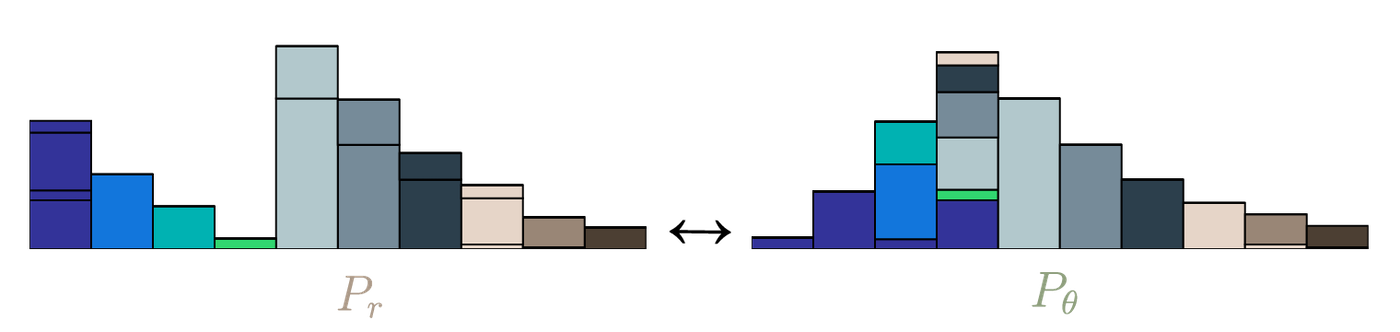
\includegraphics[width=0.5\linewidth]{img/WD.png}
      \caption{Wasserstein Distance when $p=1$: Earth Mover Distance}  
    \end{figure}
    \begin{align*}
      D_w\left[\hat{\phi}_*, \tilde{\phi}_*\right] &= \inf_{\gamma \in \Gamma} \left[\int \left\vert t_1 - t_2 \right\vert^p \gamma(t_1, t_2)\mathrm{d}t_1\mathrm{d}t_2\right]^{\frac{1}{p}}
    \end{align*}
    \begin{align*}
      \Gamma &= \left\{\gamma(t_1, t_2) ~\middle\vert~ \int\gamma(t_1,t_2)\mathrm{d}t_1 = \tilde{\phi}_*(t_2) , \int\gamma(t_1,t_2)\mathrm{d}t_2 = \hat{\phi}_*(t_1) \right\}
    \end{align*}
    when $p=1$, CDF of $\phi(t)$ is $\Phi(t)$, $D_w$ is a $\ell_1$-distance:
    \begin{align*}
      D_w\left[\hat{\phi}_*, \tilde{\phi}_*\right] &= \int\left|\hat{\Phi}(t) - \tilde{\Phi}(t)\right| \mathrm{d}t
    \end{align*}

  \end{block}

\end{column}

\separatorcolumn

\begin{column}{\colwidth}

  \begin{block}{Fast Bayesian Matching Pursuit\cite{schniter_fast_nodate} in waveform analysis}

    \begin{itemize}
      \item FBMP is a sparse regression algorithm, which origins from the field of signal processing. 
      \item Time in DAQ window is divided into time bins: $\vec{t}$, whose length is $N$. Each time bin can have 1 PE. As long as the bin width is small, the timing resolution will be retained. 
      \item Model vector: $\vec{z}$. $z_i=0\implies q_i=0$ and $\ z_i=1\implies q_i\neq0$. When $z_i$ is 0, the corresponding charge of PE in time bin $t_i$ will be 0, otherwise it may not be zero. 
      \item Linear Model: $\vec{w} = \bm{V}_\mathrm{PE}\vec{z} + \vec{\epsilon}$. This process is equivalent to $\tilde{\phi}$ convoluting with Single PE, and merely time is digitized. 
      \item 
          \begin{align*}
              \left.
              \begin{bmatrix}
                  \vec{w} \\
                  \vec{q}
              \end{bmatrix}
              \right\vert\vec{z}
              &\sim \mathrm{Normal}\left(
              \begin{bmatrix}
                  \bm{V}_\mathrm{PE}\vec{z} \\
                  \vec{z}
              \end{bmatrix}, 
              \begin{bmatrix}
                  \bm{\Sigma}_z & \bm{V}_\mathrm{PE}\bm{Z} \\
                  \bm{Z}\bm{V}_\mathrm{PE}^\intercal & \bm{Z}
              \end{bmatrix}
              \right) \\
              \bm{\Sigma}_z &= \bm{V}_\mathrm{PE}\bm{Z}\bm{V}_\mathrm{PE}^\intercal+\sigma_\epsilon^2\bm{I}
          \end{align*}
        where $\bm{Z}$ is the diagonal matrix of vector $\vec{z}$ controlling $q_i$ 
        \item $\mathcal{Z}=\{\vec{z}_j\}$ contains \textcolor{red}{$2^{N}$} model vectors
    \end{itemize}

  \end{block}

  \begin{block}{FBMP Evaluation}

    \begin{itemize}
        \item Calculation of \textcolor{red}{$2^{N}$} model vectors is impossible!
        \item Most of $p(\vec{w}|\vec{z}) \rightarrow 0$!
    \end{itemize}
    \noindent\begin{minipage}[c]{0.33\textwidth}
        \begin{figure}[H]
            \centering
                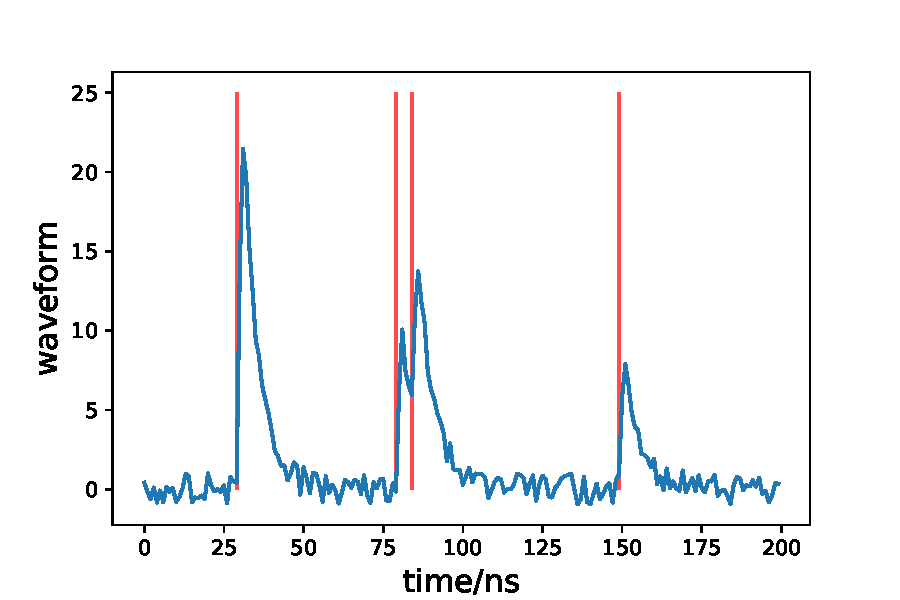
\includegraphics[width=0.95\textwidth]{img/perfect_PE.pdf}
            \caption{perfect PE matching waveform, $p(\vec{z}|\vec{w})$ hit maximum}
            \label{fig:perfect PE}
        \end{figure}
    \end{minipage}\begin{minipage}[c]{0.33\textwidth}
        \begin{figure}[H]
            \centering
                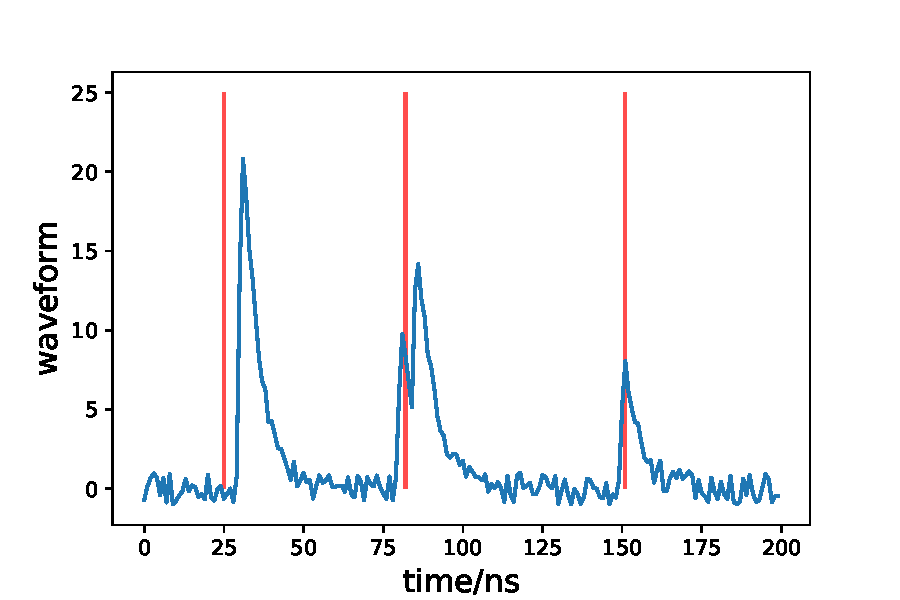
\includegraphics[width=0.95\textwidth]{img/not_so_perfect_PE.pdf}
            \caption{not so perfect, $p(\vec{z}|\vec{w})$ is smaller but still $>0$}
            \label{fig:not so perfect PE}
        \end{figure}
    \end{minipage}\begin{minipage}[c]{0.33\textwidth}
        \begin{figure}[H]
            \centering
                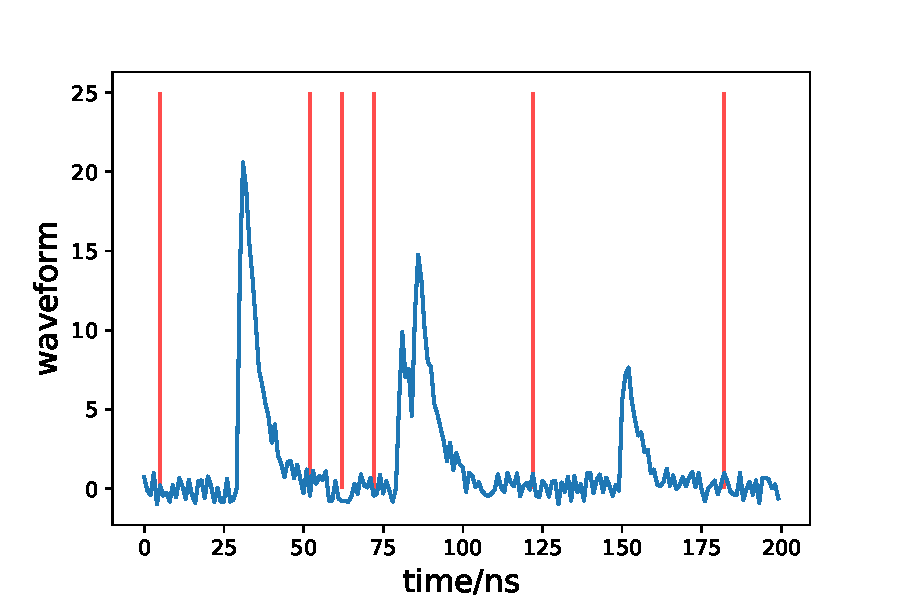
\includegraphics[width=0.95\textwidth]{img/nonsense_PE.pdf}
            \caption{Completely mismatch the waveform, $p(\vec{z}|\vec{w}) \rightarrow 0$}
            \label{fig:nonsense PE}
        \end{figure}
    \end{minipage}

    \begin{itemize}
      \item Most z can be ignored because most z does not correspond to the waveform. If we only consider the model vector z with a relatively large posterior probability, the calculation effort will be reduced. 
      \item \begin{align*}
          \log[\textcolor{red}{p(\vec{w},\vec{z})}] =& \log[p(\vec{w}|\vec{z})p(\vec{z})] \\
          =& -\frac{1}{2}(\vec{w}-\bm{V}_\mathrm{PE}\vec{z})^\intercal\bm{\Sigma}_z^{-1}(\vec{w}-\bm{V}_\mathrm{PE}\vec{z})-\frac{1}{2}\log\det\bm{\Sigma}_z \\ 
          &-\frac{N}{2}\log2\pi -\mu + \sum_{i|z_i=1}\log \frac{\mu \phi(t'_i - t_0) \Delta t'}{1-\mu \phi(t'_i - t_0) \Delta t'}
          \end{align*}
      \item A \textcolor{red}{repeated greedy search}(RGS) is performed to construct the target set $\mathcal{Z}'$, which contains only the $\vec{z}$ giving large $p(\vec{w}|\vec{z})$. 
      \begin{align*}
        p(\vec{z}|\vec{w}) &= \frac{p(\vec{w}|\vec{z})p(\vec{z})}{\sum_{\vec{z}'\in\mathcal{Z}}p(\vec{w}|\vec{z'})p(\vec{z'})} \approx \frac{p(\vec{w}|\vec{z})p(\vec{z})}{\sum_{\vec{z}'\in\mathcal{Z}'}p(\vec{w}|\vec{z'})p(\vec{z'})}
      \end{align*}
    \end{itemize}

  \end{block}

  \begin{block}{FBMP's Bayesian interface}

    \begin{itemize}
      \item PE Time: $\vec{t}$
      \item Models: $\mathcal{Z}'=\{\vec{z}_j\}$
      \item Charge: \begin{align*}
          \hat{\vec{q}}_z = E(\vec{q}|\vec{w},\vec{z}) &= \vec{z} + \bm{Z}\bm{V}_\mathrm{PE}^\intercal\bm{\Sigma}_z^{-1}(\vec{w}-\bm{V}_\mathrm{PE}\vec{z})
          \end{align*}
      \item Model's posterior probability: $p(\vec{z}|\vec{w})$
      \item The final result of FBMP is the time vector, several models, and their corresponding charge vectors. Additionally, the posterior probability of each model. In commonly used fitting methods such as Maximum likelihood estimation(MLE), the posterior distribution is approximated into delta function or normal distribution. 
    \end{itemize}
    \begin{center}
        Provides opportunity for subsequent \textcolor{red}{Bayesian} analysis! 
    \end{center}

  \end{block}

\end{column}

\separatorcolumn

\begin{column}{\colwidth}

  \begin{block}{FBMP Demonstration}

    \begin{figure}
      \centering
      \resizebox{0.8\textwidth}{!}{%% Creator: Matplotlib, PGF backend
%%
%% To include the figure in your LaTeX document, write
%%   \input{<filename>.pgf}
%%
%% Make sure the required packages are loaded in your preamble
%%   \usepackage{pgf}
%%
%% and, on pdftex
%%   \usepackage[utf8]{inputenc}\DeclareUnicodeCharacter{2212}{-}
%%
%% or, on luatex and xetex
%%   \usepackage{unicode-math}
%%
%% Figures using additional raster images can only be included by \input if
%% they are in the same directory as the main LaTeX file. For loading figures
%% from other directories you can use the `import` package
%%   \usepackage{import}
%%
%% and then include the figures with
%%   \import{<path to file>}{<filename>.pgf}
%%
%% Matplotlib used the following preamble
%%
\begingroup%
\makeatletter%
\begin{pgfpicture}%
\pgfpathrectangle{\pgfpointorigin}{\pgfqpoint{10.000000in}{10.000000in}}%
\pgfusepath{use as bounding box, clip}%
\begin{pgfscope}%
\pgfsetbuttcap%
\pgfsetmiterjoin%
\definecolor{currentfill}{rgb}{1.000000,1.000000,1.000000}%
\pgfsetfillcolor{currentfill}%
\pgfsetlinewidth{0.000000pt}%
\definecolor{currentstroke}{rgb}{1.000000,1.000000,1.000000}%
\pgfsetstrokecolor{currentstroke}%
\pgfsetdash{}{0pt}%
\pgfpathmoveto{\pgfqpoint{0.000000in}{0.000000in}}%
\pgfpathlineto{\pgfqpoint{10.000000in}{0.000000in}}%
\pgfpathlineto{\pgfqpoint{10.000000in}{10.000000in}}%
\pgfpathlineto{\pgfqpoint{0.000000in}{10.000000in}}%
\pgfpathclose%
\pgfusepath{fill}%
\end{pgfscope}%
\begin{pgfscope}%
\pgfsetbuttcap%
\pgfsetmiterjoin%
\definecolor{currentfill}{rgb}{1.000000,1.000000,1.000000}%
\pgfsetfillcolor{currentfill}%
\pgfsetlinewidth{0.000000pt}%
\definecolor{currentstroke}{rgb}{0.000000,0.000000,0.000000}%
\pgfsetstrokecolor{currentstroke}%
\pgfsetstrokeopacity{0.000000}%
\pgfsetdash{}{0pt}%
\pgfpathmoveto{\pgfqpoint{1.000000in}{2.000000in}}%
\pgfpathlineto{\pgfqpoint{9.500000in}{2.000000in}}%
\pgfpathlineto{\pgfqpoint{9.500000in}{5.000000in}}%
\pgfpathlineto{\pgfqpoint{1.000000in}{5.000000in}}%
\pgfpathclose%
\pgfusepath{fill}%
\end{pgfscope}%
\begin{pgfscope}%
\pgfpathrectangle{\pgfqpoint{1.000000in}{2.000000in}}{\pgfqpoint{8.500000in}{3.000000in}}%
\pgfusepath{clip}%
\pgfsetbuttcap%
\pgfsetroundjoin%
\pgfsetlinewidth{2.007500pt}%
\definecolor{currentstroke}{rgb}{0.000000,0.750000,0.750000}%
\pgfsetstrokecolor{currentstroke}%
\pgfsetdash{}{0pt}%
\pgfpathmoveto{\pgfqpoint{0.990000in}{3.026316in}}%
\pgfpathlineto{\pgfqpoint{9.510000in}{3.026316in}}%
\pgfusepath{stroke}%
\end{pgfscope}%
\begin{pgfscope}%
\pgfpathrectangle{\pgfqpoint{1.000000in}{2.000000in}}{\pgfqpoint{8.500000in}{3.000000in}}%
\pgfusepath{clip}%
\pgfsetrectcap%
\pgfsetroundjoin%
\pgfsetlinewidth{2.007500pt}%
\definecolor{currentstroke}{rgb}{0.000000,0.000000,1.000000}%
\pgfsetstrokecolor{currentstroke}%
\pgfsetdash{}{0pt}%
\pgfpathmoveto{\pgfqpoint{0.997329in}{2.631579in}}%
\pgfpathlineto{\pgfqpoint{1.033697in}{2.473684in}}%
\pgfpathlineto{\pgfqpoint{1.070065in}{2.710526in}}%
\pgfpathlineto{\pgfqpoint{1.179168in}{2.473684in}}%
\pgfpathlineto{\pgfqpoint{1.215536in}{2.552632in}}%
\pgfpathlineto{\pgfqpoint{1.251904in}{2.552632in}}%
\pgfpathlineto{\pgfqpoint{1.288272in}{2.631579in}}%
\pgfpathlineto{\pgfqpoint{1.324640in}{2.552632in}}%
\pgfpathlineto{\pgfqpoint{1.361008in}{2.789474in}}%
\pgfpathlineto{\pgfqpoint{1.470111in}{2.552632in}}%
\pgfpathlineto{\pgfqpoint{1.506479in}{2.631579in}}%
\pgfpathlineto{\pgfqpoint{1.542847in}{2.473684in}}%
\pgfpathlineto{\pgfqpoint{1.579215in}{2.710526in}}%
\pgfpathlineto{\pgfqpoint{1.651951in}{2.710526in}}%
\pgfpathlineto{\pgfqpoint{1.688319in}{2.552632in}}%
\pgfpathlineto{\pgfqpoint{1.724687in}{2.710526in}}%
\pgfpathlineto{\pgfqpoint{1.761054in}{2.710526in}}%
\pgfpathlineto{\pgfqpoint{1.833790in}{2.552632in}}%
\pgfpathlineto{\pgfqpoint{1.870158in}{2.710526in}}%
\pgfpathlineto{\pgfqpoint{1.906526in}{2.631579in}}%
\pgfpathlineto{\pgfqpoint{1.979262in}{2.631579in}}%
\pgfpathlineto{\pgfqpoint{2.015630in}{2.552632in}}%
\pgfpathlineto{\pgfqpoint{2.051997in}{2.710526in}}%
\pgfpathlineto{\pgfqpoint{2.088365in}{2.473684in}}%
\pgfpathlineto{\pgfqpoint{2.124733in}{2.710526in}}%
\pgfpathlineto{\pgfqpoint{2.161101in}{2.631579in}}%
\pgfpathlineto{\pgfqpoint{2.197469in}{2.631579in}}%
\pgfpathlineto{\pgfqpoint{2.233837in}{2.552632in}}%
\pgfpathlineto{\pgfqpoint{2.270205in}{2.710526in}}%
\pgfpathlineto{\pgfqpoint{2.306573in}{2.631579in}}%
\pgfpathlineto{\pgfqpoint{2.342940in}{2.789474in}}%
\pgfpathlineto{\pgfqpoint{2.379308in}{2.631579in}}%
\pgfpathlineto{\pgfqpoint{2.524780in}{2.631579in}}%
\pgfpathlineto{\pgfqpoint{2.561148in}{2.710526in}}%
\pgfpathlineto{\pgfqpoint{2.597516in}{2.710526in}}%
\pgfpathlineto{\pgfqpoint{2.633884in}{2.473684in}}%
\pgfpathlineto{\pgfqpoint{2.670251in}{2.552632in}}%
\pgfpathlineto{\pgfqpoint{2.706619in}{2.552632in}}%
\pgfpathlineto{\pgfqpoint{2.742987in}{2.710526in}}%
\pgfpathlineto{\pgfqpoint{2.779355in}{2.552632in}}%
\pgfpathlineto{\pgfqpoint{2.815723in}{2.710526in}}%
\pgfpathlineto{\pgfqpoint{2.888459in}{2.710526in}}%
\pgfpathlineto{\pgfqpoint{2.924827in}{2.631579in}}%
\pgfpathlineto{\pgfqpoint{2.961194in}{2.789474in}}%
\pgfpathlineto{\pgfqpoint{2.997562in}{2.868421in}}%
\pgfpathlineto{\pgfqpoint{3.033930in}{3.263158in}}%
\pgfpathlineto{\pgfqpoint{3.070298in}{3.184211in}}%
\pgfpathlineto{\pgfqpoint{3.106666in}{3.342105in}}%
\pgfpathlineto{\pgfqpoint{3.143034in}{3.342105in}}%
\pgfpathlineto{\pgfqpoint{3.179402in}{3.184211in}}%
\pgfpathlineto{\pgfqpoint{3.215770in}{3.342105in}}%
\pgfpathlineto{\pgfqpoint{3.252137in}{3.263158in}}%
\pgfpathlineto{\pgfqpoint{3.324873in}{3.894737in}}%
\pgfpathlineto{\pgfqpoint{3.361241in}{4.289474in}}%
\pgfpathlineto{\pgfqpoint{3.397609in}{4.368421in}}%
\pgfpathlineto{\pgfqpoint{3.433977in}{4.605263in}}%
\pgfpathlineto{\pgfqpoint{3.470345in}{4.289474in}}%
\pgfpathlineto{\pgfqpoint{3.506713in}{4.210526in}}%
\pgfpathlineto{\pgfqpoint{3.543081in}{4.052632in}}%
\pgfpathlineto{\pgfqpoint{3.579448in}{3.973684in}}%
\pgfpathlineto{\pgfqpoint{3.615816in}{3.736842in}}%
\pgfpathlineto{\pgfqpoint{3.652184in}{3.421053in}}%
\pgfpathlineto{\pgfqpoint{3.688552in}{3.421053in}}%
\pgfpathlineto{\pgfqpoint{3.724920in}{3.342105in}}%
\pgfpathlineto{\pgfqpoint{3.761288in}{3.184211in}}%
\pgfpathlineto{\pgfqpoint{3.797656in}{3.342105in}}%
\pgfpathlineto{\pgfqpoint{3.870391in}{3.973684in}}%
\pgfpathlineto{\pgfqpoint{3.906759in}{4.131579in}}%
\pgfpathlineto{\pgfqpoint{3.943127in}{3.973684in}}%
\pgfpathlineto{\pgfqpoint{4.015863in}{4.131579in}}%
\pgfpathlineto{\pgfqpoint{4.124967in}{3.657895in}}%
\pgfpathlineto{\pgfqpoint{4.161335in}{3.894737in}}%
\pgfpathlineto{\pgfqpoint{4.197702in}{3.894737in}}%
\pgfpathlineto{\pgfqpoint{4.234070in}{4.052632in}}%
\pgfpathlineto{\pgfqpoint{4.343174in}{4.289474in}}%
\pgfpathlineto{\pgfqpoint{4.379542in}{3.894737in}}%
\pgfpathlineto{\pgfqpoint{4.452278in}{3.894737in}}%
\pgfpathlineto{\pgfqpoint{4.488645in}{3.578947in}}%
\pgfpathlineto{\pgfqpoint{4.525013in}{3.421053in}}%
\pgfpathlineto{\pgfqpoint{4.561381in}{3.342105in}}%
\pgfpathlineto{\pgfqpoint{4.597749in}{3.184211in}}%
\pgfpathlineto{\pgfqpoint{4.634117in}{3.184211in}}%
\pgfpathlineto{\pgfqpoint{4.670485in}{2.947368in}}%
\pgfpathlineto{\pgfqpoint{4.706853in}{3.105263in}}%
\pgfpathlineto{\pgfqpoint{4.743221in}{2.868421in}}%
\pgfpathlineto{\pgfqpoint{4.852324in}{2.868421in}}%
\pgfpathlineto{\pgfqpoint{4.888692in}{2.789474in}}%
\pgfpathlineto{\pgfqpoint{4.925060in}{2.789474in}}%
\pgfpathlineto{\pgfqpoint{4.961428in}{2.710526in}}%
\pgfpathlineto{\pgfqpoint{4.997796in}{2.789474in}}%
\pgfpathlineto{\pgfqpoint{5.034164in}{2.710526in}}%
\pgfpathlineto{\pgfqpoint{5.070532in}{2.789474in}}%
\pgfpathlineto{\pgfqpoint{5.106899in}{2.631579in}}%
\pgfpathlineto{\pgfqpoint{5.143267in}{2.710526in}}%
\pgfpathlineto{\pgfqpoint{5.179635in}{2.631579in}}%
\pgfpathlineto{\pgfqpoint{5.216003in}{2.710526in}}%
\pgfpathlineto{\pgfqpoint{5.252371in}{2.631579in}}%
\pgfpathlineto{\pgfqpoint{5.361475in}{2.631579in}}%
\pgfpathlineto{\pgfqpoint{5.397842in}{2.473684in}}%
\pgfpathlineto{\pgfqpoint{5.434210in}{2.552632in}}%
\pgfpathlineto{\pgfqpoint{5.470578in}{2.710526in}}%
\pgfpathlineto{\pgfqpoint{5.506946in}{2.631579in}}%
\pgfpathlineto{\pgfqpoint{5.543314in}{2.631579in}}%
\pgfpathlineto{\pgfqpoint{5.579682in}{2.710526in}}%
\pgfpathlineto{\pgfqpoint{5.616050in}{2.710526in}}%
\pgfpathlineto{\pgfqpoint{5.652418in}{2.789474in}}%
\pgfpathlineto{\pgfqpoint{5.725153in}{2.631579in}}%
\pgfpathlineto{\pgfqpoint{5.761521in}{2.631579in}}%
\pgfpathlineto{\pgfqpoint{5.797889in}{2.710526in}}%
\pgfpathlineto{\pgfqpoint{5.834257in}{2.710526in}}%
\pgfpathlineto{\pgfqpoint{5.870625in}{2.552632in}}%
\pgfpathlineto{\pgfqpoint{5.906993in}{2.710526in}}%
\pgfpathlineto{\pgfqpoint{5.943361in}{2.789474in}}%
\pgfpathlineto{\pgfqpoint{5.979729in}{2.631579in}}%
\pgfpathlineto{\pgfqpoint{6.016096in}{2.631579in}}%
\pgfpathlineto{\pgfqpoint{6.052464in}{2.552632in}}%
\pgfpathlineto{\pgfqpoint{6.088832in}{2.552632in}}%
\pgfpathlineto{\pgfqpoint{6.161568in}{2.710526in}}%
\pgfpathlineto{\pgfqpoint{6.197936in}{2.631579in}}%
\pgfpathlineto{\pgfqpoint{6.234304in}{2.710526in}}%
\pgfpathlineto{\pgfqpoint{6.270672in}{2.710526in}}%
\pgfpathlineto{\pgfqpoint{6.307039in}{2.631579in}}%
\pgfpathlineto{\pgfqpoint{6.343407in}{2.710526in}}%
\pgfpathlineto{\pgfqpoint{6.379775in}{2.631579in}}%
\pgfpathlineto{\pgfqpoint{6.416143in}{2.631579in}}%
\pgfpathlineto{\pgfqpoint{6.488879in}{2.789474in}}%
\pgfpathlineto{\pgfqpoint{6.525247in}{2.552632in}}%
\pgfpathlineto{\pgfqpoint{6.597983in}{2.710526in}}%
\pgfpathlineto{\pgfqpoint{6.634350in}{2.631579in}}%
\pgfpathlineto{\pgfqpoint{6.670718in}{2.631579in}}%
\pgfpathlineto{\pgfqpoint{6.707086in}{2.789474in}}%
\pgfpathlineto{\pgfqpoint{6.743454in}{2.631579in}}%
\pgfpathlineto{\pgfqpoint{6.779822in}{2.710526in}}%
\pgfpathlineto{\pgfqpoint{6.816190in}{2.631579in}}%
\pgfpathlineto{\pgfqpoint{6.852558in}{2.473684in}}%
\pgfpathlineto{\pgfqpoint{6.888926in}{2.552632in}}%
\pgfpathlineto{\pgfqpoint{6.925293in}{2.710526in}}%
\pgfpathlineto{\pgfqpoint{6.998029in}{2.552632in}}%
\pgfpathlineto{\pgfqpoint{7.034397in}{2.789474in}}%
\pgfpathlineto{\pgfqpoint{7.070765in}{2.631579in}}%
\pgfpathlineto{\pgfqpoint{7.107133in}{2.552632in}}%
\pgfpathlineto{\pgfqpoint{7.143501in}{2.710526in}}%
\pgfpathlineto{\pgfqpoint{7.179869in}{2.710526in}}%
\pgfpathlineto{\pgfqpoint{7.216237in}{2.552632in}}%
\pgfpathlineto{\pgfqpoint{7.252604in}{2.710526in}}%
\pgfpathlineto{\pgfqpoint{7.288972in}{2.710526in}}%
\pgfpathlineto{\pgfqpoint{7.325340in}{2.631579in}}%
\pgfpathlineto{\pgfqpoint{7.361708in}{2.631579in}}%
\pgfpathlineto{\pgfqpoint{7.398076in}{2.473684in}}%
\pgfpathlineto{\pgfqpoint{7.434444in}{2.631579in}}%
\pgfpathlineto{\pgfqpoint{7.470812in}{2.631579in}}%
\pgfpathlineto{\pgfqpoint{7.507180in}{2.552632in}}%
\pgfpathlineto{\pgfqpoint{7.579915in}{2.710526in}}%
\pgfpathlineto{\pgfqpoint{7.616283in}{2.631579in}}%
\pgfpathlineto{\pgfqpoint{7.652651in}{2.473684in}}%
\pgfpathlineto{\pgfqpoint{7.689019in}{2.552632in}}%
\pgfpathlineto{\pgfqpoint{7.725387in}{2.552632in}}%
\pgfpathlineto{\pgfqpoint{7.761755in}{2.631579in}}%
\pgfpathlineto{\pgfqpoint{7.798123in}{2.552632in}}%
\pgfpathlineto{\pgfqpoint{7.834490in}{2.631579in}}%
\pgfpathlineto{\pgfqpoint{7.870858in}{2.552632in}}%
\pgfpathlineto{\pgfqpoint{7.907226in}{2.710526in}}%
\pgfpathlineto{\pgfqpoint{7.943594in}{2.631579in}}%
\pgfpathlineto{\pgfqpoint{7.979962in}{2.710526in}}%
\pgfpathlineto{\pgfqpoint{8.052698in}{2.552632in}}%
\pgfpathlineto{\pgfqpoint{8.089066in}{2.631579in}}%
\pgfpathlineto{\pgfqpoint{8.125434in}{2.789474in}}%
\pgfpathlineto{\pgfqpoint{8.161801in}{2.473684in}}%
\pgfpathlineto{\pgfqpoint{8.198169in}{2.710526in}}%
\pgfpathlineto{\pgfqpoint{8.234537in}{2.631579in}}%
\pgfpathlineto{\pgfqpoint{8.270905in}{2.473684in}}%
\pgfpathlineto{\pgfqpoint{8.307273in}{2.710526in}}%
\pgfpathlineto{\pgfqpoint{8.343641in}{2.710526in}}%
\pgfpathlineto{\pgfqpoint{8.380009in}{2.631579in}}%
\pgfpathlineto{\pgfqpoint{8.416377in}{2.631579in}}%
\pgfpathlineto{\pgfqpoint{8.452744in}{2.789474in}}%
\pgfpathlineto{\pgfqpoint{8.489112in}{2.552632in}}%
\pgfpathlineto{\pgfqpoint{8.525480in}{2.789474in}}%
\pgfpathlineto{\pgfqpoint{8.561848in}{2.789474in}}%
\pgfpathlineto{\pgfqpoint{8.598216in}{2.552632in}}%
\pgfpathlineto{\pgfqpoint{8.634584in}{2.631579in}}%
\pgfpathlineto{\pgfqpoint{8.670952in}{2.631579in}}%
\pgfpathlineto{\pgfqpoint{8.707320in}{2.710526in}}%
\pgfpathlineto{\pgfqpoint{8.743687in}{2.710526in}}%
\pgfpathlineto{\pgfqpoint{8.780055in}{2.789474in}}%
\pgfpathlineto{\pgfqpoint{8.816423in}{2.473684in}}%
\pgfpathlineto{\pgfqpoint{8.852791in}{2.710526in}}%
\pgfpathlineto{\pgfqpoint{8.889159in}{2.710526in}}%
\pgfpathlineto{\pgfqpoint{8.925527in}{2.473684in}}%
\pgfpathlineto{\pgfqpoint{8.961895in}{2.710526in}}%
\pgfpathlineto{\pgfqpoint{8.998263in}{2.552632in}}%
\pgfpathlineto{\pgfqpoint{9.034631in}{2.710526in}}%
\pgfpathlineto{\pgfqpoint{9.070998in}{2.552632in}}%
\pgfpathlineto{\pgfqpoint{9.107366in}{2.631579in}}%
\pgfpathlineto{\pgfqpoint{9.180102in}{2.631579in}}%
\pgfpathlineto{\pgfqpoint{9.216470in}{2.552632in}}%
\pgfpathlineto{\pgfqpoint{9.252838in}{2.631579in}}%
\pgfpathlineto{\pgfqpoint{9.289206in}{2.552632in}}%
\pgfpathlineto{\pgfqpoint{9.325574in}{2.710526in}}%
\pgfpathlineto{\pgfqpoint{9.361941in}{2.552632in}}%
\pgfpathlineto{\pgfqpoint{9.398309in}{2.631579in}}%
\pgfpathlineto{\pgfqpoint{9.434677in}{2.631579in}}%
\pgfpathlineto{\pgfqpoint{9.471045in}{2.789474in}}%
\pgfpathlineto{\pgfqpoint{9.507413in}{2.473684in}}%
\pgfpathlineto{\pgfqpoint{9.507413in}{2.473684in}}%
\pgfusepath{stroke}%
\end{pgfscope}%
\begin{pgfscope}%
\pgfpathrectangle{\pgfqpoint{1.000000in}{2.000000in}}{\pgfqpoint{8.500000in}{3.000000in}}%
\pgfusepath{clip}%
\pgfsetrectcap%
\pgfsetroundjoin%
\pgfsetlinewidth{2.007500pt}%
\definecolor{currentstroke}{rgb}{0.000000,0.000000,0.000000}%
\pgfsetstrokecolor{currentstroke}%
\pgfsetdash{}{0pt}%
\pgfpathmoveto{\pgfqpoint{0.997329in}{2.631579in}}%
\pgfpathlineto{\pgfqpoint{9.507413in}{2.631579in}}%
\pgfpathlineto{\pgfqpoint{9.507413in}{2.631579in}}%
\pgfusepath{stroke}%
\end{pgfscope}%
\begin{pgfscope}%
\pgfpathrectangle{\pgfqpoint{1.000000in}{2.000000in}}{\pgfqpoint{8.500000in}{3.000000in}}%
\pgfusepath{clip}%
\pgfsetrectcap%
\pgfsetroundjoin%
\pgfsetlinewidth{2.007500pt}%
\definecolor{currentstroke}{rgb}{0.000000,0.500000,0.000000}%
\pgfsetstrokecolor{currentstroke}%
\pgfsetdash{}{0pt}%
\pgfpathmoveto{\pgfqpoint{0.997329in}{2.631579in}}%
\pgfpathlineto{\pgfqpoint{2.852091in}{2.631621in}}%
\pgfpathlineto{\pgfqpoint{2.888459in}{2.636772in}}%
\pgfpathlineto{\pgfqpoint{2.924827in}{2.675369in}}%
\pgfpathlineto{\pgfqpoint{2.961194in}{2.783570in}}%
\pgfpathlineto{\pgfqpoint{3.033930in}{3.100673in}}%
\pgfpathlineto{\pgfqpoint{3.070298in}{3.213566in}}%
\pgfpathlineto{\pgfqpoint{3.106666in}{3.270650in}}%
\pgfpathlineto{\pgfqpoint{3.143034in}{3.278628in}}%
\pgfpathlineto{\pgfqpoint{3.179402in}{3.251377in}}%
\pgfpathlineto{\pgfqpoint{3.215770in}{3.228109in}}%
\pgfpathlineto{\pgfqpoint{3.252137in}{3.326269in}}%
\pgfpathlineto{\pgfqpoint{3.288505in}{3.588800in}}%
\pgfpathlineto{\pgfqpoint{3.324873in}{3.915880in}}%
\pgfpathlineto{\pgfqpoint{3.361241in}{4.186887in}}%
\pgfpathlineto{\pgfqpoint{3.397609in}{4.341049in}}%
\pgfpathlineto{\pgfqpoint{3.433977in}{4.374884in}}%
\pgfpathlineto{\pgfqpoint{3.470345in}{4.314044in}}%
\pgfpathlineto{\pgfqpoint{3.506713in}{4.191297in}}%
\pgfpathlineto{\pgfqpoint{3.543081in}{4.035518in}}%
\pgfpathlineto{\pgfqpoint{3.615816in}{3.703369in}}%
\pgfpathlineto{\pgfqpoint{3.652184in}{3.549528in}}%
\pgfpathlineto{\pgfqpoint{3.688552in}{3.410930in}}%
\pgfpathlineto{\pgfqpoint{3.724920in}{3.298529in}}%
\pgfpathlineto{\pgfqpoint{3.761288in}{3.265793in}}%
\pgfpathlineto{\pgfqpoint{3.797656in}{3.382147in}}%
\pgfpathlineto{\pgfqpoint{3.870391in}{3.851774in}}%
\pgfpathlineto{\pgfqpoint{3.906759in}{4.016316in}}%
\pgfpathlineto{\pgfqpoint{3.943127in}{4.082414in}}%
\pgfpathlineto{\pgfqpoint{3.979495in}{4.061346in}}%
\pgfpathlineto{\pgfqpoint{4.015863in}{3.978139in}}%
\pgfpathlineto{\pgfqpoint{4.052231in}{3.858261in}}%
\pgfpathlineto{\pgfqpoint{4.088599in}{3.730428in}}%
\pgfpathlineto{\pgfqpoint{4.124967in}{3.653194in}}%
\pgfpathlineto{\pgfqpoint{4.161335in}{3.687360in}}%
\pgfpathlineto{\pgfqpoint{4.197702in}{3.818735in}}%
\pgfpathlineto{\pgfqpoint{4.234070in}{3.969974in}}%
\pgfpathlineto{\pgfqpoint{4.270438in}{4.072674in}}%
\pgfpathlineto{\pgfqpoint{4.306806in}{4.099689in}}%
\pgfpathlineto{\pgfqpoint{4.343174in}{4.056101in}}%
\pgfpathlineto{\pgfqpoint{4.379542in}{3.961224in}}%
\pgfpathlineto{\pgfqpoint{4.415910in}{3.836270in}}%
\pgfpathlineto{\pgfqpoint{4.488645in}{3.561043in}}%
\pgfpathlineto{\pgfqpoint{4.525013in}{3.430885in}}%
\pgfpathlineto{\pgfqpoint{4.561381in}{3.312467in}}%
\pgfpathlineto{\pgfqpoint{4.597749in}{3.207535in}}%
\pgfpathlineto{\pgfqpoint{4.634117in}{3.116283in}}%
\pgfpathlineto{\pgfqpoint{4.670485in}{3.037995in}}%
\pgfpathlineto{\pgfqpoint{4.706853in}{2.971492in}}%
\pgfpathlineto{\pgfqpoint{4.743221in}{2.915405in}}%
\pgfpathlineto{\pgfqpoint{4.779588in}{2.868352in}}%
\pgfpathlineto{\pgfqpoint{4.815956in}{2.829023in}}%
\pgfpathlineto{\pgfqpoint{4.852324in}{2.796237in}}%
\pgfpathlineto{\pgfqpoint{4.888692in}{2.768950in}}%
\pgfpathlineto{\pgfqpoint{4.925060in}{2.746263in}}%
\pgfpathlineto{\pgfqpoint{4.961428in}{2.727408in}}%
\pgfpathlineto{\pgfqpoint{4.997796in}{2.711740in}}%
\pgfpathlineto{\pgfqpoint{5.034164in}{2.698714in}}%
\pgfpathlineto{\pgfqpoint{5.070532in}{2.687879in}}%
\pgfpathlineto{\pgfqpoint{5.106899in}{2.678859in}}%
\pgfpathlineto{\pgfqpoint{5.143267in}{2.671342in}}%
\pgfpathlineto{\pgfqpoint{5.216003in}{2.659831in}}%
\pgfpathlineto{\pgfqpoint{5.288739in}{2.651778in}}%
\pgfpathlineto{\pgfqpoint{5.361475in}{2.646113in}}%
\pgfpathlineto{\pgfqpoint{5.470578in}{2.640555in}}%
\pgfpathlineto{\pgfqpoint{5.616050in}{2.636402in}}%
\pgfpathlineto{\pgfqpoint{5.797889in}{2.633858in}}%
\pgfpathlineto{\pgfqpoint{6.125200in}{2.632197in}}%
\pgfpathlineto{\pgfqpoint{6.888926in}{2.631612in}}%
\pgfpathlineto{\pgfqpoint{9.507413in}{2.631579in}}%
\pgfpathlineto{\pgfqpoint{9.507413in}{2.631579in}}%
\pgfusepath{stroke}%
\end{pgfscope}%
\begin{pgfscope}%
\pgfsetrectcap%
\pgfsetmiterjoin%
\pgfsetlinewidth{1.003750pt}%
\definecolor{currentstroke}{rgb}{0.000000,0.000000,0.000000}%
\pgfsetstrokecolor{currentstroke}%
\pgfsetdash{}{0pt}%
\pgfpathmoveto{\pgfqpoint{1.000000in}{2.000000in}}%
\pgfpathlineto{\pgfqpoint{1.000000in}{5.000000in}}%
\pgfusepath{stroke}%
\end{pgfscope}%
\begin{pgfscope}%
\pgfsetrectcap%
\pgfsetmiterjoin%
\pgfsetlinewidth{1.003750pt}%
\definecolor{currentstroke}{rgb}{0.000000,0.000000,0.000000}%
\pgfsetstrokecolor{currentstroke}%
\pgfsetdash{}{0pt}%
\pgfpathmoveto{\pgfqpoint{9.500000in}{2.000000in}}%
\pgfpathlineto{\pgfqpoint{9.500000in}{5.000000in}}%
\pgfusepath{stroke}%
\end{pgfscope}%
\begin{pgfscope}%
\pgfsetrectcap%
\pgfsetmiterjoin%
\pgfsetlinewidth{1.003750pt}%
\definecolor{currentstroke}{rgb}{0.000000,0.000000,0.000000}%
\pgfsetstrokecolor{currentstroke}%
\pgfsetdash{}{0pt}%
\pgfpathmoveto{\pgfqpoint{1.000000in}{2.000000in}}%
\pgfpathlineto{\pgfqpoint{9.500000in}{2.000000in}}%
\pgfusepath{stroke}%
\end{pgfscope}%
\begin{pgfscope}%
\pgfsetrectcap%
\pgfsetmiterjoin%
\pgfsetlinewidth{1.003750pt}%
\definecolor{currentstroke}{rgb}{0.000000,0.000000,0.000000}%
\pgfsetstrokecolor{currentstroke}%
\pgfsetdash{}{0pt}%
\pgfpathmoveto{\pgfqpoint{1.000000in}{5.000000in}}%
\pgfpathlineto{\pgfqpoint{9.500000in}{5.000000in}}%
\pgfusepath{stroke}%
\end{pgfscope}%
\begin{pgfscope}%
\pgfpathrectangle{\pgfqpoint{1.000000in}{2.000000in}}{\pgfqpoint{8.500000in}{3.000000in}}%
\pgfusepath{clip}%
\pgfsetbuttcap%
\pgfsetroundjoin%
\pgfsetlinewidth{0.501875pt}%
\definecolor{currentstroke}{rgb}{0.000000,0.000000,0.000000}%
\pgfsetstrokecolor{currentstroke}%
\pgfsetdash{{1.000000pt}{3.000000pt}}{0.000000pt}%
\pgfpathmoveto{\pgfqpoint{1.470111in}{2.000000in}}%
\pgfpathlineto{\pgfqpoint{1.470111in}{5.000000in}}%
\pgfusepath{stroke}%
\end{pgfscope}%
\begin{pgfscope}%
\pgfsetbuttcap%
\pgfsetroundjoin%
\definecolor{currentfill}{rgb}{0.000000,0.000000,0.000000}%
\pgfsetfillcolor{currentfill}%
\pgfsetlinewidth{0.501875pt}%
\definecolor{currentstroke}{rgb}{0.000000,0.000000,0.000000}%
\pgfsetstrokecolor{currentstroke}%
\pgfsetdash{}{0pt}%
\pgfsys@defobject{currentmarker}{\pgfqpoint{0.000000in}{0.000000in}}{\pgfqpoint{0.000000in}{0.055556in}}{%
\pgfpathmoveto{\pgfqpoint{0.000000in}{0.000000in}}%
\pgfpathlineto{\pgfqpoint{0.000000in}{0.055556in}}%
\pgfusepath{stroke,fill}%
}%
\begin{pgfscope}%
\pgfsys@transformshift{1.470111in}{2.000000in}%
\pgfsys@useobject{currentmarker}{}%
\end{pgfscope}%
\end{pgfscope}%
\begin{pgfscope}%
\pgfsetbuttcap%
\pgfsetroundjoin%
\definecolor{currentfill}{rgb}{0.000000,0.000000,0.000000}%
\pgfsetfillcolor{currentfill}%
\pgfsetlinewidth{0.501875pt}%
\definecolor{currentstroke}{rgb}{0.000000,0.000000,0.000000}%
\pgfsetstrokecolor{currentstroke}%
\pgfsetdash{}{0pt}%
\pgfsys@defobject{currentmarker}{\pgfqpoint{0.000000in}{-0.055556in}}{\pgfqpoint{0.000000in}{0.000000in}}{%
\pgfpathmoveto{\pgfqpoint{0.000000in}{0.000000in}}%
\pgfpathlineto{\pgfqpoint{0.000000in}{-0.055556in}}%
\pgfusepath{stroke,fill}%
}%
\begin{pgfscope}%
\pgfsys@transformshift{1.470111in}{5.000000in}%
\pgfsys@useobject{currentmarker}{}%
\end{pgfscope}%
\end{pgfscope}%
\begin{pgfscope}%
\pgfpathrectangle{\pgfqpoint{1.000000in}{2.000000in}}{\pgfqpoint{8.500000in}{3.000000in}}%
\pgfusepath{clip}%
\pgfsetbuttcap%
\pgfsetroundjoin%
\pgfsetlinewidth{0.501875pt}%
\definecolor{currentstroke}{rgb}{0.000000,0.000000,0.000000}%
\pgfsetstrokecolor{currentstroke}%
\pgfsetdash{{1.000000pt}{3.000000pt}}{0.000000pt}%
\pgfpathmoveto{\pgfqpoint{3.288505in}{2.000000in}}%
\pgfpathlineto{\pgfqpoint{3.288505in}{5.000000in}}%
\pgfusepath{stroke}%
\end{pgfscope}%
\begin{pgfscope}%
\pgfsetbuttcap%
\pgfsetroundjoin%
\definecolor{currentfill}{rgb}{0.000000,0.000000,0.000000}%
\pgfsetfillcolor{currentfill}%
\pgfsetlinewidth{0.501875pt}%
\definecolor{currentstroke}{rgb}{0.000000,0.000000,0.000000}%
\pgfsetstrokecolor{currentstroke}%
\pgfsetdash{}{0pt}%
\pgfsys@defobject{currentmarker}{\pgfqpoint{0.000000in}{0.000000in}}{\pgfqpoint{0.000000in}{0.055556in}}{%
\pgfpathmoveto{\pgfqpoint{0.000000in}{0.000000in}}%
\pgfpathlineto{\pgfqpoint{0.000000in}{0.055556in}}%
\pgfusepath{stroke,fill}%
}%
\begin{pgfscope}%
\pgfsys@transformshift{3.288505in}{2.000000in}%
\pgfsys@useobject{currentmarker}{}%
\end{pgfscope}%
\end{pgfscope}%
\begin{pgfscope}%
\pgfsetbuttcap%
\pgfsetroundjoin%
\definecolor{currentfill}{rgb}{0.000000,0.000000,0.000000}%
\pgfsetfillcolor{currentfill}%
\pgfsetlinewidth{0.501875pt}%
\definecolor{currentstroke}{rgb}{0.000000,0.000000,0.000000}%
\pgfsetstrokecolor{currentstroke}%
\pgfsetdash{}{0pt}%
\pgfsys@defobject{currentmarker}{\pgfqpoint{0.000000in}{-0.055556in}}{\pgfqpoint{0.000000in}{0.000000in}}{%
\pgfpathmoveto{\pgfqpoint{0.000000in}{0.000000in}}%
\pgfpathlineto{\pgfqpoint{0.000000in}{-0.055556in}}%
\pgfusepath{stroke,fill}%
}%
\begin{pgfscope}%
\pgfsys@transformshift{3.288505in}{5.000000in}%
\pgfsys@useobject{currentmarker}{}%
\end{pgfscope}%
\end{pgfscope}%
\begin{pgfscope}%
\pgfpathrectangle{\pgfqpoint{1.000000in}{2.000000in}}{\pgfqpoint{8.500000in}{3.000000in}}%
\pgfusepath{clip}%
\pgfsetbuttcap%
\pgfsetroundjoin%
\pgfsetlinewidth{0.501875pt}%
\definecolor{currentstroke}{rgb}{0.000000,0.000000,0.000000}%
\pgfsetstrokecolor{currentstroke}%
\pgfsetdash{{1.000000pt}{3.000000pt}}{0.000000pt}%
\pgfpathmoveto{\pgfqpoint{5.106899in}{2.000000in}}%
\pgfpathlineto{\pgfqpoint{5.106899in}{5.000000in}}%
\pgfusepath{stroke}%
\end{pgfscope}%
\begin{pgfscope}%
\pgfsetbuttcap%
\pgfsetroundjoin%
\definecolor{currentfill}{rgb}{0.000000,0.000000,0.000000}%
\pgfsetfillcolor{currentfill}%
\pgfsetlinewidth{0.501875pt}%
\definecolor{currentstroke}{rgb}{0.000000,0.000000,0.000000}%
\pgfsetstrokecolor{currentstroke}%
\pgfsetdash{}{0pt}%
\pgfsys@defobject{currentmarker}{\pgfqpoint{0.000000in}{0.000000in}}{\pgfqpoint{0.000000in}{0.055556in}}{%
\pgfpathmoveto{\pgfqpoint{0.000000in}{0.000000in}}%
\pgfpathlineto{\pgfqpoint{0.000000in}{0.055556in}}%
\pgfusepath{stroke,fill}%
}%
\begin{pgfscope}%
\pgfsys@transformshift{5.106899in}{2.000000in}%
\pgfsys@useobject{currentmarker}{}%
\end{pgfscope}%
\end{pgfscope}%
\begin{pgfscope}%
\pgfsetbuttcap%
\pgfsetroundjoin%
\definecolor{currentfill}{rgb}{0.000000,0.000000,0.000000}%
\pgfsetfillcolor{currentfill}%
\pgfsetlinewidth{0.501875pt}%
\definecolor{currentstroke}{rgb}{0.000000,0.000000,0.000000}%
\pgfsetstrokecolor{currentstroke}%
\pgfsetdash{}{0pt}%
\pgfsys@defobject{currentmarker}{\pgfqpoint{0.000000in}{-0.055556in}}{\pgfqpoint{0.000000in}{0.000000in}}{%
\pgfpathmoveto{\pgfqpoint{0.000000in}{0.000000in}}%
\pgfpathlineto{\pgfqpoint{0.000000in}{-0.055556in}}%
\pgfusepath{stroke,fill}%
}%
\begin{pgfscope}%
\pgfsys@transformshift{5.106899in}{5.000000in}%
\pgfsys@useobject{currentmarker}{}%
\end{pgfscope}%
\end{pgfscope}%
\begin{pgfscope}%
\pgfpathrectangle{\pgfqpoint{1.000000in}{2.000000in}}{\pgfqpoint{8.500000in}{3.000000in}}%
\pgfusepath{clip}%
\pgfsetbuttcap%
\pgfsetroundjoin%
\pgfsetlinewidth{0.501875pt}%
\definecolor{currentstroke}{rgb}{0.000000,0.000000,0.000000}%
\pgfsetstrokecolor{currentstroke}%
\pgfsetdash{{1.000000pt}{3.000000pt}}{0.000000pt}%
\pgfpathmoveto{\pgfqpoint{6.925293in}{2.000000in}}%
\pgfpathlineto{\pgfqpoint{6.925293in}{5.000000in}}%
\pgfusepath{stroke}%
\end{pgfscope}%
\begin{pgfscope}%
\pgfsetbuttcap%
\pgfsetroundjoin%
\definecolor{currentfill}{rgb}{0.000000,0.000000,0.000000}%
\pgfsetfillcolor{currentfill}%
\pgfsetlinewidth{0.501875pt}%
\definecolor{currentstroke}{rgb}{0.000000,0.000000,0.000000}%
\pgfsetstrokecolor{currentstroke}%
\pgfsetdash{}{0pt}%
\pgfsys@defobject{currentmarker}{\pgfqpoint{0.000000in}{0.000000in}}{\pgfqpoint{0.000000in}{0.055556in}}{%
\pgfpathmoveto{\pgfqpoint{0.000000in}{0.000000in}}%
\pgfpathlineto{\pgfqpoint{0.000000in}{0.055556in}}%
\pgfusepath{stroke,fill}%
}%
\begin{pgfscope}%
\pgfsys@transformshift{6.925293in}{2.000000in}%
\pgfsys@useobject{currentmarker}{}%
\end{pgfscope}%
\end{pgfscope}%
\begin{pgfscope}%
\pgfsetbuttcap%
\pgfsetroundjoin%
\definecolor{currentfill}{rgb}{0.000000,0.000000,0.000000}%
\pgfsetfillcolor{currentfill}%
\pgfsetlinewidth{0.501875pt}%
\definecolor{currentstroke}{rgb}{0.000000,0.000000,0.000000}%
\pgfsetstrokecolor{currentstroke}%
\pgfsetdash{}{0pt}%
\pgfsys@defobject{currentmarker}{\pgfqpoint{0.000000in}{-0.055556in}}{\pgfqpoint{0.000000in}{0.000000in}}{%
\pgfpathmoveto{\pgfqpoint{0.000000in}{0.000000in}}%
\pgfpathlineto{\pgfqpoint{0.000000in}{-0.055556in}}%
\pgfusepath{stroke,fill}%
}%
\begin{pgfscope}%
\pgfsys@transformshift{6.925293in}{5.000000in}%
\pgfsys@useobject{currentmarker}{}%
\end{pgfscope}%
\end{pgfscope}%
\begin{pgfscope}%
\pgfpathrectangle{\pgfqpoint{1.000000in}{2.000000in}}{\pgfqpoint{8.500000in}{3.000000in}}%
\pgfusepath{clip}%
\pgfsetbuttcap%
\pgfsetroundjoin%
\pgfsetlinewidth{0.501875pt}%
\definecolor{currentstroke}{rgb}{0.000000,0.000000,0.000000}%
\pgfsetstrokecolor{currentstroke}%
\pgfsetdash{{1.000000pt}{3.000000pt}}{0.000000pt}%
\pgfpathmoveto{\pgfqpoint{8.743687in}{2.000000in}}%
\pgfpathlineto{\pgfqpoint{8.743687in}{5.000000in}}%
\pgfusepath{stroke}%
\end{pgfscope}%
\begin{pgfscope}%
\pgfsetbuttcap%
\pgfsetroundjoin%
\definecolor{currentfill}{rgb}{0.000000,0.000000,0.000000}%
\pgfsetfillcolor{currentfill}%
\pgfsetlinewidth{0.501875pt}%
\definecolor{currentstroke}{rgb}{0.000000,0.000000,0.000000}%
\pgfsetstrokecolor{currentstroke}%
\pgfsetdash{}{0pt}%
\pgfsys@defobject{currentmarker}{\pgfqpoint{0.000000in}{0.000000in}}{\pgfqpoint{0.000000in}{0.055556in}}{%
\pgfpathmoveto{\pgfqpoint{0.000000in}{0.000000in}}%
\pgfpathlineto{\pgfqpoint{0.000000in}{0.055556in}}%
\pgfusepath{stroke,fill}%
}%
\begin{pgfscope}%
\pgfsys@transformshift{8.743687in}{2.000000in}%
\pgfsys@useobject{currentmarker}{}%
\end{pgfscope}%
\end{pgfscope}%
\begin{pgfscope}%
\pgfsetbuttcap%
\pgfsetroundjoin%
\definecolor{currentfill}{rgb}{0.000000,0.000000,0.000000}%
\pgfsetfillcolor{currentfill}%
\pgfsetlinewidth{0.501875pt}%
\definecolor{currentstroke}{rgb}{0.000000,0.000000,0.000000}%
\pgfsetstrokecolor{currentstroke}%
\pgfsetdash{}{0pt}%
\pgfsys@defobject{currentmarker}{\pgfqpoint{0.000000in}{-0.055556in}}{\pgfqpoint{0.000000in}{0.000000in}}{%
\pgfpathmoveto{\pgfqpoint{0.000000in}{0.000000in}}%
\pgfpathlineto{\pgfqpoint{0.000000in}{-0.055556in}}%
\pgfusepath{stroke,fill}%
}%
\begin{pgfscope}%
\pgfsys@transformshift{8.743687in}{5.000000in}%
\pgfsys@useobject{currentmarker}{}%
\end{pgfscope}%
\end{pgfscope}%
\begin{pgfscope}%
\pgfpathrectangle{\pgfqpoint{1.000000in}{2.000000in}}{\pgfqpoint{8.500000in}{3.000000in}}%
\pgfusepath{clip}%
\pgfsetbuttcap%
\pgfsetroundjoin%
\pgfsetlinewidth{0.501875pt}%
\definecolor{currentstroke}{rgb}{0.000000,0.000000,0.000000}%
\pgfsetstrokecolor{currentstroke}%
\pgfsetdash{{1.000000pt}{3.000000pt}}{0.000000pt}%
\pgfpathmoveto{\pgfqpoint{1.000000in}{2.236842in}}%
\pgfpathlineto{\pgfqpoint{9.500000in}{2.236842in}}%
\pgfusepath{stroke}%
\end{pgfscope}%
\begin{pgfscope}%
\pgfsetbuttcap%
\pgfsetroundjoin%
\definecolor{currentfill}{rgb}{0.000000,0.000000,0.000000}%
\pgfsetfillcolor{currentfill}%
\pgfsetlinewidth{0.501875pt}%
\definecolor{currentstroke}{rgb}{0.000000,0.000000,0.000000}%
\pgfsetstrokecolor{currentstroke}%
\pgfsetdash{}{0pt}%
\pgfsys@defobject{currentmarker}{\pgfqpoint{0.000000in}{0.000000in}}{\pgfqpoint{0.055556in}{0.000000in}}{%
\pgfpathmoveto{\pgfqpoint{0.000000in}{0.000000in}}%
\pgfpathlineto{\pgfqpoint{0.055556in}{0.000000in}}%
\pgfusepath{stroke,fill}%
}%
\begin{pgfscope}%
\pgfsys@transformshift{1.000000in}{2.236842in}%
\pgfsys@useobject{currentmarker}{}%
\end{pgfscope}%
\end{pgfscope}%
\begin{pgfscope}%
\pgfsetbuttcap%
\pgfsetroundjoin%
\definecolor{currentfill}{rgb}{0.000000,0.000000,0.000000}%
\pgfsetfillcolor{currentfill}%
\pgfsetlinewidth{0.501875pt}%
\definecolor{currentstroke}{rgb}{0.000000,0.000000,0.000000}%
\pgfsetstrokecolor{currentstroke}%
\pgfsetdash{}{0pt}%
\pgfsys@defobject{currentmarker}{\pgfqpoint{-0.055556in}{0.000000in}}{\pgfqpoint{0.000000in}{0.000000in}}{%
\pgfpathmoveto{\pgfqpoint{0.000000in}{0.000000in}}%
\pgfpathlineto{\pgfqpoint{-0.055556in}{0.000000in}}%
\pgfusepath{stroke,fill}%
}%
\begin{pgfscope}%
\pgfsys@transformshift{9.500000in}{2.236842in}%
\pgfsys@useobject{currentmarker}{}%
\end{pgfscope}%
\end{pgfscope}%
\begin{pgfscope}%
\definecolor{textcolor}{rgb}{0.000000,0.000000,0.000000}%
\pgfsetstrokecolor{textcolor}%
\pgfsetfillcolor{textcolor}%
\pgftext[x=0.944444in,y=2.236842in,right,]{\color{textcolor}\sffamily\fontsize{20.000000}{24.000000}\selectfont \(\displaystyle {-5}\)}%
\end{pgfscope}%
\begin{pgfscope}%
\pgfpathrectangle{\pgfqpoint{1.000000in}{2.000000in}}{\pgfqpoint{8.500000in}{3.000000in}}%
\pgfusepath{clip}%
\pgfsetbuttcap%
\pgfsetroundjoin%
\pgfsetlinewidth{0.501875pt}%
\definecolor{currentstroke}{rgb}{0.000000,0.000000,0.000000}%
\pgfsetstrokecolor{currentstroke}%
\pgfsetdash{{1.000000pt}{3.000000pt}}{0.000000pt}%
\pgfpathmoveto{\pgfqpoint{1.000000in}{2.631579in}}%
\pgfpathlineto{\pgfqpoint{9.500000in}{2.631579in}}%
\pgfusepath{stroke}%
\end{pgfscope}%
\begin{pgfscope}%
\pgfsetbuttcap%
\pgfsetroundjoin%
\definecolor{currentfill}{rgb}{0.000000,0.000000,0.000000}%
\pgfsetfillcolor{currentfill}%
\pgfsetlinewidth{0.501875pt}%
\definecolor{currentstroke}{rgb}{0.000000,0.000000,0.000000}%
\pgfsetstrokecolor{currentstroke}%
\pgfsetdash{}{0pt}%
\pgfsys@defobject{currentmarker}{\pgfqpoint{0.000000in}{0.000000in}}{\pgfqpoint{0.055556in}{0.000000in}}{%
\pgfpathmoveto{\pgfqpoint{0.000000in}{0.000000in}}%
\pgfpathlineto{\pgfqpoint{0.055556in}{0.000000in}}%
\pgfusepath{stroke,fill}%
}%
\begin{pgfscope}%
\pgfsys@transformshift{1.000000in}{2.631579in}%
\pgfsys@useobject{currentmarker}{}%
\end{pgfscope}%
\end{pgfscope}%
\begin{pgfscope}%
\pgfsetbuttcap%
\pgfsetroundjoin%
\definecolor{currentfill}{rgb}{0.000000,0.000000,0.000000}%
\pgfsetfillcolor{currentfill}%
\pgfsetlinewidth{0.501875pt}%
\definecolor{currentstroke}{rgb}{0.000000,0.000000,0.000000}%
\pgfsetstrokecolor{currentstroke}%
\pgfsetdash{}{0pt}%
\pgfsys@defobject{currentmarker}{\pgfqpoint{-0.055556in}{0.000000in}}{\pgfqpoint{0.000000in}{0.000000in}}{%
\pgfpathmoveto{\pgfqpoint{0.000000in}{0.000000in}}%
\pgfpathlineto{\pgfqpoint{-0.055556in}{0.000000in}}%
\pgfusepath{stroke,fill}%
}%
\begin{pgfscope}%
\pgfsys@transformshift{9.500000in}{2.631579in}%
\pgfsys@useobject{currentmarker}{}%
\end{pgfscope}%
\end{pgfscope}%
\begin{pgfscope}%
\definecolor{textcolor}{rgb}{0.000000,0.000000,0.000000}%
\pgfsetstrokecolor{textcolor}%
\pgfsetfillcolor{textcolor}%
\pgftext[x=0.944444in,y=2.631579in,right,]{\color{textcolor}\sffamily\fontsize{20.000000}{24.000000}\selectfont \(\displaystyle {0}\)}%
\end{pgfscope}%
\begin{pgfscope}%
\pgfpathrectangle{\pgfqpoint{1.000000in}{2.000000in}}{\pgfqpoint{8.500000in}{3.000000in}}%
\pgfusepath{clip}%
\pgfsetbuttcap%
\pgfsetroundjoin%
\pgfsetlinewidth{0.501875pt}%
\definecolor{currentstroke}{rgb}{0.000000,0.000000,0.000000}%
\pgfsetstrokecolor{currentstroke}%
\pgfsetdash{{1.000000pt}{3.000000pt}}{0.000000pt}%
\pgfpathmoveto{\pgfqpoint{1.000000in}{3.026316in}}%
\pgfpathlineto{\pgfqpoint{9.500000in}{3.026316in}}%
\pgfusepath{stroke}%
\end{pgfscope}%
\begin{pgfscope}%
\pgfsetbuttcap%
\pgfsetroundjoin%
\definecolor{currentfill}{rgb}{0.000000,0.000000,0.000000}%
\pgfsetfillcolor{currentfill}%
\pgfsetlinewidth{0.501875pt}%
\definecolor{currentstroke}{rgb}{0.000000,0.000000,0.000000}%
\pgfsetstrokecolor{currentstroke}%
\pgfsetdash{}{0pt}%
\pgfsys@defobject{currentmarker}{\pgfqpoint{0.000000in}{0.000000in}}{\pgfqpoint{0.055556in}{0.000000in}}{%
\pgfpathmoveto{\pgfqpoint{0.000000in}{0.000000in}}%
\pgfpathlineto{\pgfqpoint{0.055556in}{0.000000in}}%
\pgfusepath{stroke,fill}%
}%
\begin{pgfscope}%
\pgfsys@transformshift{1.000000in}{3.026316in}%
\pgfsys@useobject{currentmarker}{}%
\end{pgfscope}%
\end{pgfscope}%
\begin{pgfscope}%
\pgfsetbuttcap%
\pgfsetroundjoin%
\definecolor{currentfill}{rgb}{0.000000,0.000000,0.000000}%
\pgfsetfillcolor{currentfill}%
\pgfsetlinewidth{0.501875pt}%
\definecolor{currentstroke}{rgb}{0.000000,0.000000,0.000000}%
\pgfsetstrokecolor{currentstroke}%
\pgfsetdash{}{0pt}%
\pgfsys@defobject{currentmarker}{\pgfqpoint{-0.055556in}{0.000000in}}{\pgfqpoint{0.000000in}{0.000000in}}{%
\pgfpathmoveto{\pgfqpoint{0.000000in}{0.000000in}}%
\pgfpathlineto{\pgfqpoint{-0.055556in}{0.000000in}}%
\pgfusepath{stroke,fill}%
}%
\begin{pgfscope}%
\pgfsys@transformshift{9.500000in}{3.026316in}%
\pgfsys@useobject{currentmarker}{}%
\end{pgfscope}%
\end{pgfscope}%
\begin{pgfscope}%
\definecolor{textcolor}{rgb}{0.000000,0.000000,0.000000}%
\pgfsetstrokecolor{textcolor}%
\pgfsetfillcolor{textcolor}%
\pgftext[x=0.944444in,y=3.026316in,right,]{\color{textcolor}\sffamily\fontsize{20.000000}{24.000000}\selectfont \(\displaystyle {5}\)}%
\end{pgfscope}%
\begin{pgfscope}%
\pgfpathrectangle{\pgfqpoint{1.000000in}{2.000000in}}{\pgfqpoint{8.500000in}{3.000000in}}%
\pgfusepath{clip}%
\pgfsetbuttcap%
\pgfsetroundjoin%
\pgfsetlinewidth{0.501875pt}%
\definecolor{currentstroke}{rgb}{0.000000,0.000000,0.000000}%
\pgfsetstrokecolor{currentstroke}%
\pgfsetdash{{1.000000pt}{3.000000pt}}{0.000000pt}%
\pgfpathmoveto{\pgfqpoint{1.000000in}{3.421053in}}%
\pgfpathlineto{\pgfqpoint{9.500000in}{3.421053in}}%
\pgfusepath{stroke}%
\end{pgfscope}%
\begin{pgfscope}%
\pgfsetbuttcap%
\pgfsetroundjoin%
\definecolor{currentfill}{rgb}{0.000000,0.000000,0.000000}%
\pgfsetfillcolor{currentfill}%
\pgfsetlinewidth{0.501875pt}%
\definecolor{currentstroke}{rgb}{0.000000,0.000000,0.000000}%
\pgfsetstrokecolor{currentstroke}%
\pgfsetdash{}{0pt}%
\pgfsys@defobject{currentmarker}{\pgfqpoint{0.000000in}{0.000000in}}{\pgfqpoint{0.055556in}{0.000000in}}{%
\pgfpathmoveto{\pgfqpoint{0.000000in}{0.000000in}}%
\pgfpathlineto{\pgfqpoint{0.055556in}{0.000000in}}%
\pgfusepath{stroke,fill}%
}%
\begin{pgfscope}%
\pgfsys@transformshift{1.000000in}{3.421053in}%
\pgfsys@useobject{currentmarker}{}%
\end{pgfscope}%
\end{pgfscope}%
\begin{pgfscope}%
\pgfsetbuttcap%
\pgfsetroundjoin%
\definecolor{currentfill}{rgb}{0.000000,0.000000,0.000000}%
\pgfsetfillcolor{currentfill}%
\pgfsetlinewidth{0.501875pt}%
\definecolor{currentstroke}{rgb}{0.000000,0.000000,0.000000}%
\pgfsetstrokecolor{currentstroke}%
\pgfsetdash{}{0pt}%
\pgfsys@defobject{currentmarker}{\pgfqpoint{-0.055556in}{0.000000in}}{\pgfqpoint{0.000000in}{0.000000in}}{%
\pgfpathmoveto{\pgfqpoint{0.000000in}{0.000000in}}%
\pgfpathlineto{\pgfqpoint{-0.055556in}{0.000000in}}%
\pgfusepath{stroke,fill}%
}%
\begin{pgfscope}%
\pgfsys@transformshift{9.500000in}{3.421053in}%
\pgfsys@useobject{currentmarker}{}%
\end{pgfscope}%
\end{pgfscope}%
\begin{pgfscope}%
\definecolor{textcolor}{rgb}{0.000000,0.000000,0.000000}%
\pgfsetstrokecolor{textcolor}%
\pgfsetfillcolor{textcolor}%
\pgftext[x=0.944444in,y=3.421053in,right,]{\color{textcolor}\sffamily\fontsize{20.000000}{24.000000}\selectfont \(\displaystyle {10}\)}%
\end{pgfscope}%
\begin{pgfscope}%
\pgfpathrectangle{\pgfqpoint{1.000000in}{2.000000in}}{\pgfqpoint{8.500000in}{3.000000in}}%
\pgfusepath{clip}%
\pgfsetbuttcap%
\pgfsetroundjoin%
\pgfsetlinewidth{0.501875pt}%
\definecolor{currentstroke}{rgb}{0.000000,0.000000,0.000000}%
\pgfsetstrokecolor{currentstroke}%
\pgfsetdash{{1.000000pt}{3.000000pt}}{0.000000pt}%
\pgfpathmoveto{\pgfqpoint{1.000000in}{3.815789in}}%
\pgfpathlineto{\pgfqpoint{9.500000in}{3.815789in}}%
\pgfusepath{stroke}%
\end{pgfscope}%
\begin{pgfscope}%
\pgfsetbuttcap%
\pgfsetroundjoin%
\definecolor{currentfill}{rgb}{0.000000,0.000000,0.000000}%
\pgfsetfillcolor{currentfill}%
\pgfsetlinewidth{0.501875pt}%
\definecolor{currentstroke}{rgb}{0.000000,0.000000,0.000000}%
\pgfsetstrokecolor{currentstroke}%
\pgfsetdash{}{0pt}%
\pgfsys@defobject{currentmarker}{\pgfqpoint{0.000000in}{0.000000in}}{\pgfqpoint{0.055556in}{0.000000in}}{%
\pgfpathmoveto{\pgfqpoint{0.000000in}{0.000000in}}%
\pgfpathlineto{\pgfqpoint{0.055556in}{0.000000in}}%
\pgfusepath{stroke,fill}%
}%
\begin{pgfscope}%
\pgfsys@transformshift{1.000000in}{3.815789in}%
\pgfsys@useobject{currentmarker}{}%
\end{pgfscope}%
\end{pgfscope}%
\begin{pgfscope}%
\pgfsetbuttcap%
\pgfsetroundjoin%
\definecolor{currentfill}{rgb}{0.000000,0.000000,0.000000}%
\pgfsetfillcolor{currentfill}%
\pgfsetlinewidth{0.501875pt}%
\definecolor{currentstroke}{rgb}{0.000000,0.000000,0.000000}%
\pgfsetstrokecolor{currentstroke}%
\pgfsetdash{}{0pt}%
\pgfsys@defobject{currentmarker}{\pgfqpoint{-0.055556in}{0.000000in}}{\pgfqpoint{0.000000in}{0.000000in}}{%
\pgfpathmoveto{\pgfqpoint{0.000000in}{0.000000in}}%
\pgfpathlineto{\pgfqpoint{-0.055556in}{0.000000in}}%
\pgfusepath{stroke,fill}%
}%
\begin{pgfscope}%
\pgfsys@transformshift{9.500000in}{3.815789in}%
\pgfsys@useobject{currentmarker}{}%
\end{pgfscope}%
\end{pgfscope}%
\begin{pgfscope}%
\definecolor{textcolor}{rgb}{0.000000,0.000000,0.000000}%
\pgfsetstrokecolor{textcolor}%
\pgfsetfillcolor{textcolor}%
\pgftext[x=0.944444in,y=3.815789in,right,]{\color{textcolor}\sffamily\fontsize{20.000000}{24.000000}\selectfont \(\displaystyle {15}\)}%
\end{pgfscope}%
\begin{pgfscope}%
\pgfpathrectangle{\pgfqpoint{1.000000in}{2.000000in}}{\pgfqpoint{8.500000in}{3.000000in}}%
\pgfusepath{clip}%
\pgfsetbuttcap%
\pgfsetroundjoin%
\pgfsetlinewidth{0.501875pt}%
\definecolor{currentstroke}{rgb}{0.000000,0.000000,0.000000}%
\pgfsetstrokecolor{currentstroke}%
\pgfsetdash{{1.000000pt}{3.000000pt}}{0.000000pt}%
\pgfpathmoveto{\pgfqpoint{1.000000in}{4.210526in}}%
\pgfpathlineto{\pgfqpoint{9.500000in}{4.210526in}}%
\pgfusepath{stroke}%
\end{pgfscope}%
\begin{pgfscope}%
\pgfsetbuttcap%
\pgfsetroundjoin%
\definecolor{currentfill}{rgb}{0.000000,0.000000,0.000000}%
\pgfsetfillcolor{currentfill}%
\pgfsetlinewidth{0.501875pt}%
\definecolor{currentstroke}{rgb}{0.000000,0.000000,0.000000}%
\pgfsetstrokecolor{currentstroke}%
\pgfsetdash{}{0pt}%
\pgfsys@defobject{currentmarker}{\pgfqpoint{0.000000in}{0.000000in}}{\pgfqpoint{0.055556in}{0.000000in}}{%
\pgfpathmoveto{\pgfqpoint{0.000000in}{0.000000in}}%
\pgfpathlineto{\pgfqpoint{0.055556in}{0.000000in}}%
\pgfusepath{stroke,fill}%
}%
\begin{pgfscope}%
\pgfsys@transformshift{1.000000in}{4.210526in}%
\pgfsys@useobject{currentmarker}{}%
\end{pgfscope}%
\end{pgfscope}%
\begin{pgfscope}%
\pgfsetbuttcap%
\pgfsetroundjoin%
\definecolor{currentfill}{rgb}{0.000000,0.000000,0.000000}%
\pgfsetfillcolor{currentfill}%
\pgfsetlinewidth{0.501875pt}%
\definecolor{currentstroke}{rgb}{0.000000,0.000000,0.000000}%
\pgfsetstrokecolor{currentstroke}%
\pgfsetdash{}{0pt}%
\pgfsys@defobject{currentmarker}{\pgfqpoint{-0.055556in}{0.000000in}}{\pgfqpoint{0.000000in}{0.000000in}}{%
\pgfpathmoveto{\pgfqpoint{0.000000in}{0.000000in}}%
\pgfpathlineto{\pgfqpoint{-0.055556in}{0.000000in}}%
\pgfusepath{stroke,fill}%
}%
\begin{pgfscope}%
\pgfsys@transformshift{9.500000in}{4.210526in}%
\pgfsys@useobject{currentmarker}{}%
\end{pgfscope}%
\end{pgfscope}%
\begin{pgfscope}%
\definecolor{textcolor}{rgb}{0.000000,0.000000,0.000000}%
\pgfsetstrokecolor{textcolor}%
\pgfsetfillcolor{textcolor}%
\pgftext[x=0.944444in,y=4.210526in,right,]{\color{textcolor}\sffamily\fontsize{20.000000}{24.000000}\selectfont \(\displaystyle {20}\)}%
\end{pgfscope}%
\begin{pgfscope}%
\pgfpathrectangle{\pgfqpoint{1.000000in}{2.000000in}}{\pgfqpoint{8.500000in}{3.000000in}}%
\pgfusepath{clip}%
\pgfsetbuttcap%
\pgfsetroundjoin%
\pgfsetlinewidth{0.501875pt}%
\definecolor{currentstroke}{rgb}{0.000000,0.000000,0.000000}%
\pgfsetstrokecolor{currentstroke}%
\pgfsetdash{{1.000000pt}{3.000000pt}}{0.000000pt}%
\pgfpathmoveto{\pgfqpoint{1.000000in}{4.605263in}}%
\pgfpathlineto{\pgfqpoint{9.500000in}{4.605263in}}%
\pgfusepath{stroke}%
\end{pgfscope}%
\begin{pgfscope}%
\pgfsetbuttcap%
\pgfsetroundjoin%
\definecolor{currentfill}{rgb}{0.000000,0.000000,0.000000}%
\pgfsetfillcolor{currentfill}%
\pgfsetlinewidth{0.501875pt}%
\definecolor{currentstroke}{rgb}{0.000000,0.000000,0.000000}%
\pgfsetstrokecolor{currentstroke}%
\pgfsetdash{}{0pt}%
\pgfsys@defobject{currentmarker}{\pgfqpoint{0.000000in}{0.000000in}}{\pgfqpoint{0.055556in}{0.000000in}}{%
\pgfpathmoveto{\pgfqpoint{0.000000in}{0.000000in}}%
\pgfpathlineto{\pgfqpoint{0.055556in}{0.000000in}}%
\pgfusepath{stroke,fill}%
}%
\begin{pgfscope}%
\pgfsys@transformshift{1.000000in}{4.605263in}%
\pgfsys@useobject{currentmarker}{}%
\end{pgfscope}%
\end{pgfscope}%
\begin{pgfscope}%
\pgfsetbuttcap%
\pgfsetroundjoin%
\definecolor{currentfill}{rgb}{0.000000,0.000000,0.000000}%
\pgfsetfillcolor{currentfill}%
\pgfsetlinewidth{0.501875pt}%
\definecolor{currentstroke}{rgb}{0.000000,0.000000,0.000000}%
\pgfsetstrokecolor{currentstroke}%
\pgfsetdash{}{0pt}%
\pgfsys@defobject{currentmarker}{\pgfqpoint{-0.055556in}{0.000000in}}{\pgfqpoint{0.000000in}{0.000000in}}{%
\pgfpathmoveto{\pgfqpoint{0.000000in}{0.000000in}}%
\pgfpathlineto{\pgfqpoint{-0.055556in}{0.000000in}}%
\pgfusepath{stroke,fill}%
}%
\begin{pgfscope}%
\pgfsys@transformshift{9.500000in}{4.605263in}%
\pgfsys@useobject{currentmarker}{}%
\end{pgfscope}%
\end{pgfscope}%
\begin{pgfscope}%
\definecolor{textcolor}{rgb}{0.000000,0.000000,0.000000}%
\pgfsetstrokecolor{textcolor}%
\pgfsetfillcolor{textcolor}%
\pgftext[x=0.944444in,y=4.605263in,right,]{\color{textcolor}\sffamily\fontsize{20.000000}{24.000000}\selectfont \(\displaystyle {25}\)}%
\end{pgfscope}%
\begin{pgfscope}%
\pgfpathrectangle{\pgfqpoint{1.000000in}{2.000000in}}{\pgfqpoint{8.500000in}{3.000000in}}%
\pgfusepath{clip}%
\pgfsetbuttcap%
\pgfsetroundjoin%
\pgfsetlinewidth{0.501875pt}%
\definecolor{currentstroke}{rgb}{0.000000,0.000000,0.000000}%
\pgfsetstrokecolor{currentstroke}%
\pgfsetdash{{1.000000pt}{3.000000pt}}{0.000000pt}%
\pgfpathmoveto{\pgfqpoint{1.000000in}{5.000000in}}%
\pgfpathlineto{\pgfqpoint{9.500000in}{5.000000in}}%
\pgfusepath{stroke}%
\end{pgfscope}%
\begin{pgfscope}%
\pgfsetbuttcap%
\pgfsetroundjoin%
\definecolor{currentfill}{rgb}{0.000000,0.000000,0.000000}%
\pgfsetfillcolor{currentfill}%
\pgfsetlinewidth{0.501875pt}%
\definecolor{currentstroke}{rgb}{0.000000,0.000000,0.000000}%
\pgfsetstrokecolor{currentstroke}%
\pgfsetdash{}{0pt}%
\pgfsys@defobject{currentmarker}{\pgfqpoint{0.000000in}{0.000000in}}{\pgfqpoint{0.055556in}{0.000000in}}{%
\pgfpathmoveto{\pgfqpoint{0.000000in}{0.000000in}}%
\pgfpathlineto{\pgfqpoint{0.055556in}{0.000000in}}%
\pgfusepath{stroke,fill}%
}%
\begin{pgfscope}%
\pgfsys@transformshift{1.000000in}{5.000000in}%
\pgfsys@useobject{currentmarker}{}%
\end{pgfscope}%
\end{pgfscope}%
\begin{pgfscope}%
\pgfsetbuttcap%
\pgfsetroundjoin%
\definecolor{currentfill}{rgb}{0.000000,0.000000,0.000000}%
\pgfsetfillcolor{currentfill}%
\pgfsetlinewidth{0.501875pt}%
\definecolor{currentstroke}{rgb}{0.000000,0.000000,0.000000}%
\pgfsetstrokecolor{currentstroke}%
\pgfsetdash{}{0pt}%
\pgfsys@defobject{currentmarker}{\pgfqpoint{-0.055556in}{0.000000in}}{\pgfqpoint{0.000000in}{0.000000in}}{%
\pgfpathmoveto{\pgfqpoint{0.000000in}{0.000000in}}%
\pgfpathlineto{\pgfqpoint{-0.055556in}{0.000000in}}%
\pgfusepath{stroke,fill}%
}%
\begin{pgfscope}%
\pgfsys@transformshift{9.500000in}{5.000000in}%
\pgfsys@useobject{currentmarker}{}%
\end{pgfscope}%
\end{pgfscope}%
\begin{pgfscope}%
\definecolor{textcolor}{rgb}{0.000000,0.000000,0.000000}%
\pgfsetstrokecolor{textcolor}%
\pgfsetfillcolor{textcolor}%
\pgftext[x=0.944444in,y=5.000000in,right,]{\color{textcolor}\sffamily\fontsize{20.000000}{24.000000}\selectfont \(\displaystyle {30}\)}%
\end{pgfscope}%
\begin{pgfscope}%
\definecolor{textcolor}{rgb}{0.000000,0.000000,0.000000}%
\pgfsetstrokecolor{textcolor}%
\pgfsetfillcolor{textcolor}%
\pgftext[x=0.518849in,y=3.500000in,,bottom,rotate=90.000000]{\color{textcolor}\sffamily\fontsize{20.000000}{24.000000}\selectfont \(\displaystyle Voltage/\mathrm{mV}\)}%
\end{pgfscope}%
\begin{pgfscope}%
\pgfsetbuttcap%
\pgfsetmiterjoin%
\definecolor{currentfill}{rgb}{1.000000,1.000000,1.000000}%
\pgfsetfillcolor{currentfill}%
\pgfsetlinewidth{1.003750pt}%
\definecolor{currentstroke}{rgb}{0.000000,0.000000,0.000000}%
\pgfsetstrokecolor{currentstroke}%
\pgfsetdash{}{0pt}%
\pgfpathmoveto{\pgfqpoint{6.615623in}{2.837936in}}%
\pgfpathlineto{\pgfqpoint{9.333333in}{2.837936in}}%
\pgfpathlineto{\pgfqpoint{9.333333in}{4.833333in}}%
\pgfpathlineto{\pgfqpoint{6.615623in}{4.833333in}}%
\pgfpathclose%
\pgfusepath{stroke,fill}%
\end{pgfscope}%
\begin{pgfscope}%
\pgfsetrectcap%
\pgfsetroundjoin%
\pgfsetlinewidth{2.007500pt}%
\definecolor{currentstroke}{rgb}{0.000000,0.000000,1.000000}%
\pgfsetstrokecolor{currentstroke}%
\pgfsetdash{}{0pt}%
\pgfpathmoveto{\pgfqpoint{6.848957in}{4.576697in}}%
\pgfpathlineto{\pgfqpoint{7.315623in}{4.576697in}}%
\pgfusepath{stroke}%
\end{pgfscope}%
\begin{pgfscope}%
\definecolor{textcolor}{rgb}{0.000000,0.000000,0.000000}%
\pgfsetstrokecolor{textcolor}%
\pgfsetfillcolor{textcolor}%
\pgftext[x=7.682290in,y=4.460031in,left,base]{\color{textcolor}\sffamily\fontsize{24.000000}{28.800000}\selectfont origin wave}%
\end{pgfscope}%
\begin{pgfscope}%
\pgfsetrectcap%
\pgfsetroundjoin%
\pgfsetlinewidth{2.007500pt}%
\definecolor{currentstroke}{rgb}{0.000000,0.000000,0.000000}%
\pgfsetstrokecolor{currentstroke}%
\pgfsetdash{}{0pt}%
\pgfpathmoveto{\pgfqpoint{6.848957in}{4.102848in}}%
\pgfpathlineto{\pgfqpoint{7.315623in}{4.102848in}}%
\pgfusepath{stroke}%
\end{pgfscope}%
\begin{pgfscope}%
\definecolor{textcolor}{rgb}{0.000000,0.000000,0.000000}%
\pgfsetstrokecolor{textcolor}%
\pgfsetfillcolor{textcolor}%
\pgftext[x=7.682290in,y=3.986181in,left,base]{\color{textcolor}\sffamily\fontsize{24.000000}{28.800000}\selectfont truth wave}%
\end{pgfscope}%
\begin{pgfscope}%
\pgfsetrectcap%
\pgfsetroundjoin%
\pgfsetlinewidth{2.007500pt}%
\definecolor{currentstroke}{rgb}{0.000000,0.500000,0.000000}%
\pgfsetstrokecolor{currentstroke}%
\pgfsetdash{}{0pt}%
\pgfpathmoveto{\pgfqpoint{6.848957in}{3.628998in}}%
\pgfpathlineto{\pgfqpoint{7.315623in}{3.628998in}}%
\pgfusepath{stroke}%
\end{pgfscope}%
\begin{pgfscope}%
\definecolor{textcolor}{rgb}{0.000000,0.000000,0.000000}%
\pgfsetstrokecolor{textcolor}%
\pgfsetfillcolor{textcolor}%
\pgftext[x=7.682290in,y=3.512332in,left,base]{\color{textcolor}\sffamily\fontsize{24.000000}{28.800000}\selectfont recon wave}%
\end{pgfscope}%
\begin{pgfscope}%
\pgfsetbuttcap%
\pgfsetroundjoin%
\pgfsetlinewidth{2.007500pt}%
\definecolor{currentstroke}{rgb}{0.000000,0.750000,0.750000}%
\pgfsetstrokecolor{currentstroke}%
\pgfsetdash{}{0pt}%
\pgfpathmoveto{\pgfqpoint{6.848957in}{3.155149in}}%
\pgfpathlineto{\pgfqpoint{7.082290in}{3.155149in}}%
\pgfpathlineto{\pgfqpoint{7.315623in}{3.155149in}}%
\pgfusepath{stroke}%
\end{pgfscope}%
\begin{pgfscope}%
\definecolor{textcolor}{rgb}{0.000000,0.000000,0.000000}%
\pgfsetstrokecolor{textcolor}%
\pgfsetfillcolor{textcolor}%
\pgftext[x=7.682290in,y=3.038482in,left,base]{\color{textcolor}\sffamily\fontsize{24.000000}{28.800000}\selectfont threshold}%
\end{pgfscope}%
\begin{pgfscope}%
\pgfsetbuttcap%
\pgfsetmiterjoin%
\definecolor{currentfill}{rgb}{1.000000,1.000000,1.000000}%
\pgfsetfillcolor{currentfill}%
\pgfsetlinewidth{0.000000pt}%
\definecolor{currentstroke}{rgb}{0.000000,0.000000,0.000000}%
\pgfsetstrokecolor{currentstroke}%
\pgfsetstrokeopacity{0.000000}%
\pgfsetdash{}{0pt}%
\pgfpathmoveto{\pgfqpoint{1.000000in}{5.000000in}}%
\pgfpathlineto{\pgfqpoint{9.500000in}{5.000000in}}%
\pgfpathlineto{\pgfqpoint{9.500000in}{7.000000in}}%
\pgfpathlineto{\pgfqpoint{1.000000in}{7.000000in}}%
\pgfpathclose%
\pgfusepath{fill}%
\end{pgfscope}%
\begin{pgfscope}%
\pgfpathrectangle{\pgfqpoint{1.000000in}{5.000000in}}{\pgfqpoint{8.500000in}{2.000000in}}%
\pgfusepath{clip}%
\pgfsetbuttcap%
\pgfsetroundjoin%
\pgfsetlinewidth{2.007500pt}%
\definecolor{currentstroke}{rgb}{0.000000,0.500000,0.000000}%
\pgfsetstrokecolor{currentstroke}%
\pgfsetdash{}{0pt}%
\pgfpathmoveto{\pgfqpoint{2.818394in}{5.000000in}}%
\pgfpathlineto{\pgfqpoint{2.818394in}{5.819050in}}%
\pgfusepath{stroke}%
\end{pgfscope}%
\begin{pgfscope}%
\pgfpathrectangle{\pgfqpoint{1.000000in}{5.000000in}}{\pgfqpoint{8.500000in}{2.000000in}}%
\pgfusepath{clip}%
\pgfsetbuttcap%
\pgfsetroundjoin%
\pgfsetlinewidth{2.007500pt}%
\definecolor{currentstroke}{rgb}{0.000000,0.500000,0.000000}%
\pgfsetstrokecolor{currentstroke}%
\pgfsetdash{}{0pt}%
\pgfpathmoveto{\pgfqpoint{3.145231in}{5.000000in}}%
\pgfpathlineto{\pgfqpoint{3.145231in}{6.818182in}}%
\pgfusepath{stroke}%
\end{pgfscope}%
\begin{pgfscope}%
\pgfpathrectangle{\pgfqpoint{1.000000in}{5.000000in}}{\pgfqpoint{8.500000in}{2.000000in}}%
\pgfusepath{clip}%
\pgfsetbuttcap%
\pgfsetroundjoin%
\pgfsetlinewidth{2.007500pt}%
\definecolor{currentstroke}{rgb}{0.000000,0.500000,0.000000}%
\pgfsetstrokecolor{currentstroke}%
\pgfsetdash{}{0pt}%
\pgfpathmoveto{\pgfqpoint{3.667065in}{5.000000in}}%
\pgfpathlineto{\pgfqpoint{3.667065in}{6.512864in}}%
\pgfusepath{stroke}%
\end{pgfscope}%
\begin{pgfscope}%
\pgfpathrectangle{\pgfqpoint{1.000000in}{5.000000in}}{\pgfqpoint{8.500000in}{2.000000in}}%
\pgfusepath{clip}%
\pgfsetbuttcap%
\pgfsetroundjoin%
\pgfsetlinewidth{2.007500pt}%
\definecolor{currentstroke}{rgb}{0.000000,0.500000,0.000000}%
\pgfsetstrokecolor{currentstroke}%
\pgfsetdash{}{0pt}%
\pgfpathmoveto{\pgfqpoint{4.044818in}{5.000000in}}%
\pgfpathlineto{\pgfqpoint{4.044818in}{6.403836in}}%
\pgfusepath{stroke}%
\end{pgfscope}%
\begin{pgfscope}%
\pgfsetrectcap%
\pgfsetmiterjoin%
\pgfsetlinewidth{1.003750pt}%
\definecolor{currentstroke}{rgb}{0.000000,0.000000,0.000000}%
\pgfsetstrokecolor{currentstroke}%
\pgfsetdash{}{0pt}%
\pgfpathmoveto{\pgfqpoint{1.000000in}{5.000000in}}%
\pgfpathlineto{\pgfqpoint{1.000000in}{7.000000in}}%
\pgfusepath{stroke}%
\end{pgfscope}%
\begin{pgfscope}%
\pgfsetrectcap%
\pgfsetmiterjoin%
\pgfsetlinewidth{1.003750pt}%
\definecolor{currentstroke}{rgb}{0.000000,0.000000,0.000000}%
\pgfsetstrokecolor{currentstroke}%
\pgfsetdash{}{0pt}%
\pgfpathmoveto{\pgfqpoint{9.500000in}{5.000000in}}%
\pgfpathlineto{\pgfqpoint{9.500000in}{7.000000in}}%
\pgfusepath{stroke}%
\end{pgfscope}%
\begin{pgfscope}%
\pgfsetrectcap%
\pgfsetmiterjoin%
\pgfsetlinewidth{1.003750pt}%
\definecolor{currentstroke}{rgb}{0.000000,0.000000,0.000000}%
\pgfsetstrokecolor{currentstroke}%
\pgfsetdash{}{0pt}%
\pgfpathmoveto{\pgfqpoint{1.000000in}{5.000000in}}%
\pgfpathlineto{\pgfqpoint{9.500000in}{5.000000in}}%
\pgfusepath{stroke}%
\end{pgfscope}%
\begin{pgfscope}%
\pgfsetrectcap%
\pgfsetmiterjoin%
\pgfsetlinewidth{1.003750pt}%
\definecolor{currentstroke}{rgb}{0.000000,0.000000,0.000000}%
\pgfsetstrokecolor{currentstroke}%
\pgfsetdash{}{0pt}%
\pgfpathmoveto{\pgfqpoint{1.000000in}{7.000000in}}%
\pgfpathlineto{\pgfqpoint{9.500000in}{7.000000in}}%
\pgfusepath{stroke}%
\end{pgfscope}%
\begin{pgfscope}%
\pgfpathrectangle{\pgfqpoint{1.000000in}{5.000000in}}{\pgfqpoint{8.500000in}{2.000000in}}%
\pgfusepath{clip}%
\pgfsetbuttcap%
\pgfsetroundjoin%
\pgfsetlinewidth{0.501875pt}%
\definecolor{currentstroke}{rgb}{0.000000,0.000000,0.000000}%
\pgfsetstrokecolor{currentstroke}%
\pgfsetdash{{1.000000pt}{3.000000pt}}{0.000000pt}%
\pgfpathmoveto{\pgfqpoint{1.470111in}{5.000000in}}%
\pgfpathlineto{\pgfqpoint{1.470111in}{7.000000in}}%
\pgfusepath{stroke}%
\end{pgfscope}%
\begin{pgfscope}%
\pgfsetbuttcap%
\pgfsetroundjoin%
\definecolor{currentfill}{rgb}{0.000000,0.000000,0.000000}%
\pgfsetfillcolor{currentfill}%
\pgfsetlinewidth{0.501875pt}%
\definecolor{currentstroke}{rgb}{0.000000,0.000000,0.000000}%
\pgfsetstrokecolor{currentstroke}%
\pgfsetdash{}{0pt}%
\pgfsys@defobject{currentmarker}{\pgfqpoint{0.000000in}{0.000000in}}{\pgfqpoint{0.000000in}{0.055556in}}{%
\pgfpathmoveto{\pgfqpoint{0.000000in}{0.000000in}}%
\pgfpathlineto{\pgfqpoint{0.000000in}{0.055556in}}%
\pgfusepath{stroke,fill}%
}%
\begin{pgfscope}%
\pgfsys@transformshift{1.470111in}{5.000000in}%
\pgfsys@useobject{currentmarker}{}%
\end{pgfscope}%
\end{pgfscope}%
\begin{pgfscope}%
\pgfsetbuttcap%
\pgfsetroundjoin%
\definecolor{currentfill}{rgb}{0.000000,0.000000,0.000000}%
\pgfsetfillcolor{currentfill}%
\pgfsetlinewidth{0.501875pt}%
\definecolor{currentstroke}{rgb}{0.000000,0.000000,0.000000}%
\pgfsetstrokecolor{currentstroke}%
\pgfsetdash{}{0pt}%
\pgfsys@defobject{currentmarker}{\pgfqpoint{0.000000in}{-0.055556in}}{\pgfqpoint{0.000000in}{0.000000in}}{%
\pgfpathmoveto{\pgfqpoint{0.000000in}{0.000000in}}%
\pgfpathlineto{\pgfqpoint{0.000000in}{-0.055556in}}%
\pgfusepath{stroke,fill}%
}%
\begin{pgfscope}%
\pgfsys@transformshift{1.470111in}{7.000000in}%
\pgfsys@useobject{currentmarker}{}%
\end{pgfscope}%
\end{pgfscope}%
\begin{pgfscope}%
\pgfpathrectangle{\pgfqpoint{1.000000in}{5.000000in}}{\pgfqpoint{8.500000in}{2.000000in}}%
\pgfusepath{clip}%
\pgfsetbuttcap%
\pgfsetroundjoin%
\pgfsetlinewidth{0.501875pt}%
\definecolor{currentstroke}{rgb}{0.000000,0.000000,0.000000}%
\pgfsetstrokecolor{currentstroke}%
\pgfsetdash{{1.000000pt}{3.000000pt}}{0.000000pt}%
\pgfpathmoveto{\pgfqpoint{3.288505in}{5.000000in}}%
\pgfpathlineto{\pgfqpoint{3.288505in}{7.000000in}}%
\pgfusepath{stroke}%
\end{pgfscope}%
\begin{pgfscope}%
\pgfsetbuttcap%
\pgfsetroundjoin%
\definecolor{currentfill}{rgb}{0.000000,0.000000,0.000000}%
\pgfsetfillcolor{currentfill}%
\pgfsetlinewidth{0.501875pt}%
\definecolor{currentstroke}{rgb}{0.000000,0.000000,0.000000}%
\pgfsetstrokecolor{currentstroke}%
\pgfsetdash{}{0pt}%
\pgfsys@defobject{currentmarker}{\pgfqpoint{0.000000in}{0.000000in}}{\pgfqpoint{0.000000in}{0.055556in}}{%
\pgfpathmoveto{\pgfqpoint{0.000000in}{0.000000in}}%
\pgfpathlineto{\pgfqpoint{0.000000in}{0.055556in}}%
\pgfusepath{stroke,fill}%
}%
\begin{pgfscope}%
\pgfsys@transformshift{3.288505in}{5.000000in}%
\pgfsys@useobject{currentmarker}{}%
\end{pgfscope}%
\end{pgfscope}%
\begin{pgfscope}%
\pgfsetbuttcap%
\pgfsetroundjoin%
\definecolor{currentfill}{rgb}{0.000000,0.000000,0.000000}%
\pgfsetfillcolor{currentfill}%
\pgfsetlinewidth{0.501875pt}%
\definecolor{currentstroke}{rgb}{0.000000,0.000000,0.000000}%
\pgfsetstrokecolor{currentstroke}%
\pgfsetdash{}{0pt}%
\pgfsys@defobject{currentmarker}{\pgfqpoint{0.000000in}{-0.055556in}}{\pgfqpoint{0.000000in}{0.000000in}}{%
\pgfpathmoveto{\pgfqpoint{0.000000in}{0.000000in}}%
\pgfpathlineto{\pgfqpoint{0.000000in}{-0.055556in}}%
\pgfusepath{stroke,fill}%
}%
\begin{pgfscope}%
\pgfsys@transformshift{3.288505in}{7.000000in}%
\pgfsys@useobject{currentmarker}{}%
\end{pgfscope}%
\end{pgfscope}%
\begin{pgfscope}%
\pgfpathrectangle{\pgfqpoint{1.000000in}{5.000000in}}{\pgfqpoint{8.500000in}{2.000000in}}%
\pgfusepath{clip}%
\pgfsetbuttcap%
\pgfsetroundjoin%
\pgfsetlinewidth{0.501875pt}%
\definecolor{currentstroke}{rgb}{0.000000,0.000000,0.000000}%
\pgfsetstrokecolor{currentstroke}%
\pgfsetdash{{1.000000pt}{3.000000pt}}{0.000000pt}%
\pgfpathmoveto{\pgfqpoint{5.106899in}{5.000000in}}%
\pgfpathlineto{\pgfqpoint{5.106899in}{7.000000in}}%
\pgfusepath{stroke}%
\end{pgfscope}%
\begin{pgfscope}%
\pgfsetbuttcap%
\pgfsetroundjoin%
\definecolor{currentfill}{rgb}{0.000000,0.000000,0.000000}%
\pgfsetfillcolor{currentfill}%
\pgfsetlinewidth{0.501875pt}%
\definecolor{currentstroke}{rgb}{0.000000,0.000000,0.000000}%
\pgfsetstrokecolor{currentstroke}%
\pgfsetdash{}{0pt}%
\pgfsys@defobject{currentmarker}{\pgfqpoint{0.000000in}{0.000000in}}{\pgfqpoint{0.000000in}{0.055556in}}{%
\pgfpathmoveto{\pgfqpoint{0.000000in}{0.000000in}}%
\pgfpathlineto{\pgfqpoint{0.000000in}{0.055556in}}%
\pgfusepath{stroke,fill}%
}%
\begin{pgfscope}%
\pgfsys@transformshift{5.106899in}{5.000000in}%
\pgfsys@useobject{currentmarker}{}%
\end{pgfscope}%
\end{pgfscope}%
\begin{pgfscope}%
\pgfsetbuttcap%
\pgfsetroundjoin%
\definecolor{currentfill}{rgb}{0.000000,0.000000,0.000000}%
\pgfsetfillcolor{currentfill}%
\pgfsetlinewidth{0.501875pt}%
\definecolor{currentstroke}{rgb}{0.000000,0.000000,0.000000}%
\pgfsetstrokecolor{currentstroke}%
\pgfsetdash{}{0pt}%
\pgfsys@defobject{currentmarker}{\pgfqpoint{0.000000in}{-0.055556in}}{\pgfqpoint{0.000000in}{0.000000in}}{%
\pgfpathmoveto{\pgfqpoint{0.000000in}{0.000000in}}%
\pgfpathlineto{\pgfqpoint{0.000000in}{-0.055556in}}%
\pgfusepath{stroke,fill}%
}%
\begin{pgfscope}%
\pgfsys@transformshift{5.106899in}{7.000000in}%
\pgfsys@useobject{currentmarker}{}%
\end{pgfscope}%
\end{pgfscope}%
\begin{pgfscope}%
\pgfpathrectangle{\pgfqpoint{1.000000in}{5.000000in}}{\pgfqpoint{8.500000in}{2.000000in}}%
\pgfusepath{clip}%
\pgfsetbuttcap%
\pgfsetroundjoin%
\pgfsetlinewidth{0.501875pt}%
\definecolor{currentstroke}{rgb}{0.000000,0.000000,0.000000}%
\pgfsetstrokecolor{currentstroke}%
\pgfsetdash{{1.000000pt}{3.000000pt}}{0.000000pt}%
\pgfpathmoveto{\pgfqpoint{6.925293in}{5.000000in}}%
\pgfpathlineto{\pgfqpoint{6.925293in}{7.000000in}}%
\pgfusepath{stroke}%
\end{pgfscope}%
\begin{pgfscope}%
\pgfsetbuttcap%
\pgfsetroundjoin%
\definecolor{currentfill}{rgb}{0.000000,0.000000,0.000000}%
\pgfsetfillcolor{currentfill}%
\pgfsetlinewidth{0.501875pt}%
\definecolor{currentstroke}{rgb}{0.000000,0.000000,0.000000}%
\pgfsetstrokecolor{currentstroke}%
\pgfsetdash{}{0pt}%
\pgfsys@defobject{currentmarker}{\pgfqpoint{0.000000in}{0.000000in}}{\pgfqpoint{0.000000in}{0.055556in}}{%
\pgfpathmoveto{\pgfqpoint{0.000000in}{0.000000in}}%
\pgfpathlineto{\pgfqpoint{0.000000in}{0.055556in}}%
\pgfusepath{stroke,fill}%
}%
\begin{pgfscope}%
\pgfsys@transformshift{6.925293in}{5.000000in}%
\pgfsys@useobject{currentmarker}{}%
\end{pgfscope}%
\end{pgfscope}%
\begin{pgfscope}%
\pgfsetbuttcap%
\pgfsetroundjoin%
\definecolor{currentfill}{rgb}{0.000000,0.000000,0.000000}%
\pgfsetfillcolor{currentfill}%
\pgfsetlinewidth{0.501875pt}%
\definecolor{currentstroke}{rgb}{0.000000,0.000000,0.000000}%
\pgfsetstrokecolor{currentstroke}%
\pgfsetdash{}{0pt}%
\pgfsys@defobject{currentmarker}{\pgfqpoint{0.000000in}{-0.055556in}}{\pgfqpoint{0.000000in}{0.000000in}}{%
\pgfpathmoveto{\pgfqpoint{0.000000in}{0.000000in}}%
\pgfpathlineto{\pgfqpoint{0.000000in}{-0.055556in}}%
\pgfusepath{stroke,fill}%
}%
\begin{pgfscope}%
\pgfsys@transformshift{6.925293in}{7.000000in}%
\pgfsys@useobject{currentmarker}{}%
\end{pgfscope}%
\end{pgfscope}%
\begin{pgfscope}%
\pgfpathrectangle{\pgfqpoint{1.000000in}{5.000000in}}{\pgfqpoint{8.500000in}{2.000000in}}%
\pgfusepath{clip}%
\pgfsetbuttcap%
\pgfsetroundjoin%
\pgfsetlinewidth{0.501875pt}%
\definecolor{currentstroke}{rgb}{0.000000,0.000000,0.000000}%
\pgfsetstrokecolor{currentstroke}%
\pgfsetdash{{1.000000pt}{3.000000pt}}{0.000000pt}%
\pgfpathmoveto{\pgfqpoint{8.743687in}{5.000000in}}%
\pgfpathlineto{\pgfqpoint{8.743687in}{7.000000in}}%
\pgfusepath{stroke}%
\end{pgfscope}%
\begin{pgfscope}%
\pgfsetbuttcap%
\pgfsetroundjoin%
\definecolor{currentfill}{rgb}{0.000000,0.000000,0.000000}%
\pgfsetfillcolor{currentfill}%
\pgfsetlinewidth{0.501875pt}%
\definecolor{currentstroke}{rgb}{0.000000,0.000000,0.000000}%
\pgfsetstrokecolor{currentstroke}%
\pgfsetdash{}{0pt}%
\pgfsys@defobject{currentmarker}{\pgfqpoint{0.000000in}{0.000000in}}{\pgfqpoint{0.000000in}{0.055556in}}{%
\pgfpathmoveto{\pgfqpoint{0.000000in}{0.000000in}}%
\pgfpathlineto{\pgfqpoint{0.000000in}{0.055556in}}%
\pgfusepath{stroke,fill}%
}%
\begin{pgfscope}%
\pgfsys@transformshift{8.743687in}{5.000000in}%
\pgfsys@useobject{currentmarker}{}%
\end{pgfscope}%
\end{pgfscope}%
\begin{pgfscope}%
\pgfsetbuttcap%
\pgfsetroundjoin%
\definecolor{currentfill}{rgb}{0.000000,0.000000,0.000000}%
\pgfsetfillcolor{currentfill}%
\pgfsetlinewidth{0.501875pt}%
\definecolor{currentstroke}{rgb}{0.000000,0.000000,0.000000}%
\pgfsetstrokecolor{currentstroke}%
\pgfsetdash{}{0pt}%
\pgfsys@defobject{currentmarker}{\pgfqpoint{0.000000in}{-0.055556in}}{\pgfqpoint{0.000000in}{0.000000in}}{%
\pgfpathmoveto{\pgfqpoint{0.000000in}{0.000000in}}%
\pgfpathlineto{\pgfqpoint{0.000000in}{-0.055556in}}%
\pgfusepath{stroke,fill}%
}%
\begin{pgfscope}%
\pgfsys@transformshift{8.743687in}{7.000000in}%
\pgfsys@useobject{currentmarker}{}%
\end{pgfscope}%
\end{pgfscope}%
\begin{pgfscope}%
\pgfpathrectangle{\pgfqpoint{1.000000in}{5.000000in}}{\pgfqpoint{8.500000in}{2.000000in}}%
\pgfusepath{clip}%
\pgfsetbuttcap%
\pgfsetroundjoin%
\pgfsetlinewidth{0.501875pt}%
\definecolor{currentstroke}{rgb}{0.000000,0.000000,0.000000}%
\pgfsetstrokecolor{currentstroke}%
\pgfsetdash{{1.000000pt}{3.000000pt}}{0.000000pt}%
\pgfpathmoveto{\pgfqpoint{1.000000in}{5.000000in}}%
\pgfpathlineto{\pgfqpoint{9.500000in}{5.000000in}}%
\pgfusepath{stroke}%
\end{pgfscope}%
\begin{pgfscope}%
\pgfsetbuttcap%
\pgfsetroundjoin%
\definecolor{currentfill}{rgb}{0.000000,0.000000,0.000000}%
\pgfsetfillcolor{currentfill}%
\pgfsetlinewidth{0.501875pt}%
\definecolor{currentstroke}{rgb}{0.000000,0.000000,0.000000}%
\pgfsetstrokecolor{currentstroke}%
\pgfsetdash{}{0pt}%
\pgfsys@defobject{currentmarker}{\pgfqpoint{0.000000in}{0.000000in}}{\pgfqpoint{0.055556in}{0.000000in}}{%
\pgfpathmoveto{\pgfqpoint{0.000000in}{0.000000in}}%
\pgfpathlineto{\pgfqpoint{0.055556in}{0.000000in}}%
\pgfusepath{stroke,fill}%
}%
\begin{pgfscope}%
\pgfsys@transformshift{1.000000in}{5.000000in}%
\pgfsys@useobject{currentmarker}{}%
\end{pgfscope}%
\end{pgfscope}%
\begin{pgfscope}%
\pgfsetbuttcap%
\pgfsetroundjoin%
\definecolor{currentfill}{rgb}{0.000000,0.000000,0.000000}%
\pgfsetfillcolor{currentfill}%
\pgfsetlinewidth{0.501875pt}%
\definecolor{currentstroke}{rgb}{0.000000,0.000000,0.000000}%
\pgfsetstrokecolor{currentstroke}%
\pgfsetdash{}{0pt}%
\pgfsys@defobject{currentmarker}{\pgfqpoint{-0.055556in}{0.000000in}}{\pgfqpoint{0.000000in}{0.000000in}}{%
\pgfpathmoveto{\pgfqpoint{0.000000in}{0.000000in}}%
\pgfpathlineto{\pgfqpoint{-0.055556in}{0.000000in}}%
\pgfusepath{stroke,fill}%
}%
\begin{pgfscope}%
\pgfsys@transformshift{9.500000in}{5.000000in}%
\pgfsys@useobject{currentmarker}{}%
\end{pgfscope}%
\end{pgfscope}%
\begin{pgfscope}%
\definecolor{textcolor}{rgb}{0.000000,0.000000,0.000000}%
\pgfsetstrokecolor{textcolor}%
\pgfsetfillcolor{textcolor}%
\pgftext[x=0.944444in,y=5.000000in,right,]{\color{textcolor}\sffamily\fontsize{20.000000}{24.000000}\selectfont \(\displaystyle {0}\)}%
\end{pgfscope}%
\begin{pgfscope}%
\pgfpathrectangle{\pgfqpoint{1.000000in}{5.000000in}}{\pgfqpoint{8.500000in}{2.000000in}}%
\pgfusepath{clip}%
\pgfsetbuttcap%
\pgfsetroundjoin%
\pgfsetlinewidth{0.501875pt}%
\definecolor{currentstroke}{rgb}{0.000000,0.000000,0.000000}%
\pgfsetstrokecolor{currentstroke}%
\pgfsetdash{{1.000000pt}{3.000000pt}}{0.000000pt}%
\pgfpathmoveto{\pgfqpoint{1.000000in}{5.399785in}}%
\pgfpathlineto{\pgfqpoint{9.500000in}{5.399785in}}%
\pgfusepath{stroke}%
\end{pgfscope}%
\begin{pgfscope}%
\pgfsetbuttcap%
\pgfsetroundjoin%
\definecolor{currentfill}{rgb}{0.000000,0.000000,0.000000}%
\pgfsetfillcolor{currentfill}%
\pgfsetlinewidth{0.501875pt}%
\definecolor{currentstroke}{rgb}{0.000000,0.000000,0.000000}%
\pgfsetstrokecolor{currentstroke}%
\pgfsetdash{}{0pt}%
\pgfsys@defobject{currentmarker}{\pgfqpoint{0.000000in}{0.000000in}}{\pgfqpoint{0.055556in}{0.000000in}}{%
\pgfpathmoveto{\pgfqpoint{0.000000in}{0.000000in}}%
\pgfpathlineto{\pgfqpoint{0.055556in}{0.000000in}}%
\pgfusepath{stroke,fill}%
}%
\begin{pgfscope}%
\pgfsys@transformshift{1.000000in}{5.399785in}%
\pgfsys@useobject{currentmarker}{}%
\end{pgfscope}%
\end{pgfscope}%
\begin{pgfscope}%
\pgfsetbuttcap%
\pgfsetroundjoin%
\definecolor{currentfill}{rgb}{0.000000,0.000000,0.000000}%
\pgfsetfillcolor{currentfill}%
\pgfsetlinewidth{0.501875pt}%
\definecolor{currentstroke}{rgb}{0.000000,0.000000,0.000000}%
\pgfsetstrokecolor{currentstroke}%
\pgfsetdash{}{0pt}%
\pgfsys@defobject{currentmarker}{\pgfqpoint{-0.055556in}{0.000000in}}{\pgfqpoint{0.000000in}{0.000000in}}{%
\pgfpathmoveto{\pgfqpoint{0.000000in}{0.000000in}}%
\pgfpathlineto{\pgfqpoint{-0.055556in}{0.000000in}}%
\pgfusepath{stroke,fill}%
}%
\begin{pgfscope}%
\pgfsys@transformshift{9.500000in}{5.399785in}%
\pgfsys@useobject{currentmarker}{}%
\end{pgfscope}%
\end{pgfscope}%
\begin{pgfscope}%
\definecolor{textcolor}{rgb}{0.000000,0.000000,0.000000}%
\pgfsetstrokecolor{textcolor}%
\pgfsetfillcolor{textcolor}%
\pgftext[x=0.944444in,y=5.399785in,right,]{\color{textcolor}\sffamily\fontsize{20.000000}{24.000000}\selectfont \(\displaystyle {50}\)}%
\end{pgfscope}%
\begin{pgfscope}%
\pgfpathrectangle{\pgfqpoint{1.000000in}{5.000000in}}{\pgfqpoint{8.500000in}{2.000000in}}%
\pgfusepath{clip}%
\pgfsetbuttcap%
\pgfsetroundjoin%
\pgfsetlinewidth{0.501875pt}%
\definecolor{currentstroke}{rgb}{0.000000,0.000000,0.000000}%
\pgfsetstrokecolor{currentstroke}%
\pgfsetdash{{1.000000pt}{3.000000pt}}{0.000000pt}%
\pgfpathmoveto{\pgfqpoint{1.000000in}{5.799569in}}%
\pgfpathlineto{\pgfqpoint{9.500000in}{5.799569in}}%
\pgfusepath{stroke}%
\end{pgfscope}%
\begin{pgfscope}%
\pgfsetbuttcap%
\pgfsetroundjoin%
\definecolor{currentfill}{rgb}{0.000000,0.000000,0.000000}%
\pgfsetfillcolor{currentfill}%
\pgfsetlinewidth{0.501875pt}%
\definecolor{currentstroke}{rgb}{0.000000,0.000000,0.000000}%
\pgfsetstrokecolor{currentstroke}%
\pgfsetdash{}{0pt}%
\pgfsys@defobject{currentmarker}{\pgfqpoint{0.000000in}{0.000000in}}{\pgfqpoint{0.055556in}{0.000000in}}{%
\pgfpathmoveto{\pgfqpoint{0.000000in}{0.000000in}}%
\pgfpathlineto{\pgfqpoint{0.055556in}{0.000000in}}%
\pgfusepath{stroke,fill}%
}%
\begin{pgfscope}%
\pgfsys@transformshift{1.000000in}{5.799569in}%
\pgfsys@useobject{currentmarker}{}%
\end{pgfscope}%
\end{pgfscope}%
\begin{pgfscope}%
\pgfsetbuttcap%
\pgfsetroundjoin%
\definecolor{currentfill}{rgb}{0.000000,0.000000,0.000000}%
\pgfsetfillcolor{currentfill}%
\pgfsetlinewidth{0.501875pt}%
\definecolor{currentstroke}{rgb}{0.000000,0.000000,0.000000}%
\pgfsetstrokecolor{currentstroke}%
\pgfsetdash{}{0pt}%
\pgfsys@defobject{currentmarker}{\pgfqpoint{-0.055556in}{0.000000in}}{\pgfqpoint{0.000000in}{0.000000in}}{%
\pgfpathmoveto{\pgfqpoint{0.000000in}{0.000000in}}%
\pgfpathlineto{\pgfqpoint{-0.055556in}{0.000000in}}%
\pgfusepath{stroke,fill}%
}%
\begin{pgfscope}%
\pgfsys@transformshift{9.500000in}{5.799569in}%
\pgfsys@useobject{currentmarker}{}%
\end{pgfscope}%
\end{pgfscope}%
\begin{pgfscope}%
\definecolor{textcolor}{rgb}{0.000000,0.000000,0.000000}%
\pgfsetstrokecolor{textcolor}%
\pgfsetfillcolor{textcolor}%
\pgftext[x=0.944444in,y=5.799569in,right,]{\color{textcolor}\sffamily\fontsize{20.000000}{24.000000}\selectfont \(\displaystyle {100}\)}%
\end{pgfscope}%
\begin{pgfscope}%
\pgfpathrectangle{\pgfqpoint{1.000000in}{5.000000in}}{\pgfqpoint{8.500000in}{2.000000in}}%
\pgfusepath{clip}%
\pgfsetbuttcap%
\pgfsetroundjoin%
\pgfsetlinewidth{0.501875pt}%
\definecolor{currentstroke}{rgb}{0.000000,0.000000,0.000000}%
\pgfsetstrokecolor{currentstroke}%
\pgfsetdash{{1.000000pt}{3.000000pt}}{0.000000pt}%
\pgfpathmoveto{\pgfqpoint{1.000000in}{6.199354in}}%
\pgfpathlineto{\pgfqpoint{9.500000in}{6.199354in}}%
\pgfusepath{stroke}%
\end{pgfscope}%
\begin{pgfscope}%
\pgfsetbuttcap%
\pgfsetroundjoin%
\definecolor{currentfill}{rgb}{0.000000,0.000000,0.000000}%
\pgfsetfillcolor{currentfill}%
\pgfsetlinewidth{0.501875pt}%
\definecolor{currentstroke}{rgb}{0.000000,0.000000,0.000000}%
\pgfsetstrokecolor{currentstroke}%
\pgfsetdash{}{0pt}%
\pgfsys@defobject{currentmarker}{\pgfqpoint{0.000000in}{0.000000in}}{\pgfqpoint{0.055556in}{0.000000in}}{%
\pgfpathmoveto{\pgfqpoint{0.000000in}{0.000000in}}%
\pgfpathlineto{\pgfqpoint{0.055556in}{0.000000in}}%
\pgfusepath{stroke,fill}%
}%
\begin{pgfscope}%
\pgfsys@transformshift{1.000000in}{6.199354in}%
\pgfsys@useobject{currentmarker}{}%
\end{pgfscope}%
\end{pgfscope}%
\begin{pgfscope}%
\pgfsetbuttcap%
\pgfsetroundjoin%
\definecolor{currentfill}{rgb}{0.000000,0.000000,0.000000}%
\pgfsetfillcolor{currentfill}%
\pgfsetlinewidth{0.501875pt}%
\definecolor{currentstroke}{rgb}{0.000000,0.000000,0.000000}%
\pgfsetstrokecolor{currentstroke}%
\pgfsetdash{}{0pt}%
\pgfsys@defobject{currentmarker}{\pgfqpoint{-0.055556in}{0.000000in}}{\pgfqpoint{0.000000in}{0.000000in}}{%
\pgfpathmoveto{\pgfqpoint{0.000000in}{0.000000in}}%
\pgfpathlineto{\pgfqpoint{-0.055556in}{0.000000in}}%
\pgfusepath{stroke,fill}%
}%
\begin{pgfscope}%
\pgfsys@transformshift{9.500000in}{6.199354in}%
\pgfsys@useobject{currentmarker}{}%
\end{pgfscope}%
\end{pgfscope}%
\begin{pgfscope}%
\definecolor{textcolor}{rgb}{0.000000,0.000000,0.000000}%
\pgfsetstrokecolor{textcolor}%
\pgfsetfillcolor{textcolor}%
\pgftext[x=0.944444in,y=6.199354in,right,]{\color{textcolor}\sffamily\fontsize{20.000000}{24.000000}\selectfont \(\displaystyle {150}\)}%
\end{pgfscope}%
\begin{pgfscope}%
\pgfpathrectangle{\pgfqpoint{1.000000in}{5.000000in}}{\pgfqpoint{8.500000in}{2.000000in}}%
\pgfusepath{clip}%
\pgfsetbuttcap%
\pgfsetroundjoin%
\pgfsetlinewidth{0.501875pt}%
\definecolor{currentstroke}{rgb}{0.000000,0.000000,0.000000}%
\pgfsetstrokecolor{currentstroke}%
\pgfsetdash{{1.000000pt}{3.000000pt}}{0.000000pt}%
\pgfpathmoveto{\pgfqpoint{1.000000in}{6.599138in}}%
\pgfpathlineto{\pgfqpoint{9.500000in}{6.599138in}}%
\pgfusepath{stroke}%
\end{pgfscope}%
\begin{pgfscope}%
\pgfsetbuttcap%
\pgfsetroundjoin%
\definecolor{currentfill}{rgb}{0.000000,0.000000,0.000000}%
\pgfsetfillcolor{currentfill}%
\pgfsetlinewidth{0.501875pt}%
\definecolor{currentstroke}{rgb}{0.000000,0.000000,0.000000}%
\pgfsetstrokecolor{currentstroke}%
\pgfsetdash{}{0pt}%
\pgfsys@defobject{currentmarker}{\pgfqpoint{0.000000in}{0.000000in}}{\pgfqpoint{0.055556in}{0.000000in}}{%
\pgfpathmoveto{\pgfqpoint{0.000000in}{0.000000in}}%
\pgfpathlineto{\pgfqpoint{0.055556in}{0.000000in}}%
\pgfusepath{stroke,fill}%
}%
\begin{pgfscope}%
\pgfsys@transformshift{1.000000in}{6.599138in}%
\pgfsys@useobject{currentmarker}{}%
\end{pgfscope}%
\end{pgfscope}%
\begin{pgfscope}%
\pgfsetbuttcap%
\pgfsetroundjoin%
\definecolor{currentfill}{rgb}{0.000000,0.000000,0.000000}%
\pgfsetfillcolor{currentfill}%
\pgfsetlinewidth{0.501875pt}%
\definecolor{currentstroke}{rgb}{0.000000,0.000000,0.000000}%
\pgfsetstrokecolor{currentstroke}%
\pgfsetdash{}{0pt}%
\pgfsys@defobject{currentmarker}{\pgfqpoint{-0.055556in}{0.000000in}}{\pgfqpoint{0.000000in}{0.000000in}}{%
\pgfpathmoveto{\pgfqpoint{0.000000in}{0.000000in}}%
\pgfpathlineto{\pgfqpoint{-0.055556in}{0.000000in}}%
\pgfusepath{stroke,fill}%
}%
\begin{pgfscope}%
\pgfsys@transformshift{9.500000in}{6.599138in}%
\pgfsys@useobject{currentmarker}{}%
\end{pgfscope}%
\end{pgfscope}%
\begin{pgfscope}%
\definecolor{textcolor}{rgb}{0.000000,0.000000,0.000000}%
\pgfsetstrokecolor{textcolor}%
\pgfsetfillcolor{textcolor}%
\pgftext[x=0.944444in,y=6.599138in,right,]{\color{textcolor}\sffamily\fontsize{20.000000}{24.000000}\selectfont \(\displaystyle {200}\)}%
\end{pgfscope}%
\begin{pgfscope}%
\definecolor{textcolor}{rgb}{0.000000,0.000000,0.000000}%
\pgfsetstrokecolor{textcolor}%
\pgfsetfillcolor{textcolor}%
\pgftext[x=0.478678in,y=6.000000in,,bottom,rotate=90.000000]{\color{textcolor}\sffamily\fontsize{20.000000}{24.000000}\selectfont \(\displaystyle Charge/\mathrm{mV}\cdot\mathrm{ns}\)}%
\end{pgfscope}%
\begin{pgfscope}%
\pgfsetbuttcap%
\pgfsetmiterjoin%
\definecolor{currentfill}{rgb}{1.000000,1.000000,1.000000}%
\pgfsetfillcolor{currentfill}%
\pgfsetlinewidth{1.003750pt}%
\definecolor{currentstroke}{rgb}{0.000000,0.000000,0.000000}%
\pgfsetstrokecolor{currentstroke}%
\pgfsetdash{}{0pt}%
\pgfpathmoveto{\pgfqpoint{6.406069in}{6.259484in}}%
\pgfpathlineto{\pgfqpoint{9.333333in}{6.259484in}}%
\pgfpathlineto{\pgfqpoint{9.333333in}{6.833333in}}%
\pgfpathlineto{\pgfqpoint{6.406069in}{6.833333in}}%
\pgfpathclose%
\pgfusepath{stroke,fill}%
\end{pgfscope}%
\begin{pgfscope}%
\pgfsetbuttcap%
\pgfsetroundjoin%
\pgfsetlinewidth{2.007500pt}%
\definecolor{currentstroke}{rgb}{0.000000,0.500000,0.000000}%
\pgfsetstrokecolor{currentstroke}%
\pgfsetdash{}{0pt}%
\pgfpathmoveto{\pgfqpoint{6.639402in}{6.576697in}}%
\pgfpathlineto{\pgfqpoint{6.872736in}{6.576697in}}%
\pgfpathlineto{\pgfqpoint{7.106069in}{6.576697in}}%
\pgfusepath{stroke}%
\end{pgfscope}%
\begin{pgfscope}%
\definecolor{textcolor}{rgb}{0.000000,0.000000,0.000000}%
\pgfsetstrokecolor{textcolor}%
\pgfsetfillcolor{textcolor}%
\pgftext[x=7.472736in,y=6.460031in,left,base]{\color{textcolor}\sffamily\fontsize{24.000000}{28.800000}\selectfont truth Charge}%
\end{pgfscope}%
\begin{pgfscope}%
\pgfsetbuttcap%
\pgfsetmiterjoin%
\definecolor{currentfill}{rgb}{1.000000,1.000000,1.000000}%
\pgfsetfillcolor{currentfill}%
\pgfsetlinewidth{0.000000pt}%
\definecolor{currentstroke}{rgb}{0.000000,0.000000,0.000000}%
\pgfsetstrokecolor{currentstroke}%
\pgfsetstrokeopacity{0.000000}%
\pgfsetdash{}{0pt}%
\pgfpathmoveto{\pgfqpoint{1.000000in}{7.000000in}}%
\pgfpathlineto{\pgfqpoint{9.500000in}{7.000000in}}%
\pgfpathlineto{\pgfqpoint{9.500000in}{9.000000in}}%
\pgfpathlineto{\pgfqpoint{1.000000in}{9.000000in}}%
\pgfpathclose%
\pgfusepath{fill}%
\end{pgfscope}%
\begin{pgfscope}%
\pgfpathrectangle{\pgfqpoint{1.000000in}{7.000000in}}{\pgfqpoint{8.500000in}{2.000000in}}%
\pgfusepath{clip}%
\pgfsetbuttcap%
\pgfsetroundjoin%
\pgfsetlinewidth{2.007500pt}%
\definecolor{currentstroke}{rgb}{0.750000,0.750000,0.000000}%
\pgfsetstrokecolor{currentstroke}%
\pgfsetdash{}{0pt}%
\pgfpathmoveto{\pgfqpoint{2.815723in}{7.000000in}}%
\pgfpathlineto{\pgfqpoint{2.815723in}{7.275137in}}%
\pgfusepath{stroke}%
\end{pgfscope}%
\begin{pgfscope}%
\pgfpathrectangle{\pgfqpoint{1.000000in}{7.000000in}}{\pgfqpoint{8.500000in}{2.000000in}}%
\pgfusepath{clip}%
\pgfsetbuttcap%
\pgfsetroundjoin%
\pgfsetlinewidth{2.007500pt}%
\definecolor{currentstroke}{rgb}{0.750000,0.750000,0.000000}%
\pgfsetstrokecolor{currentstroke}%
\pgfsetdash{}{0pt}%
\pgfpathmoveto{\pgfqpoint{2.852091in}{7.000000in}}%
\pgfpathlineto{\pgfqpoint{2.852091in}{7.476925in}}%
\pgfusepath{stroke}%
\end{pgfscope}%
\begin{pgfscope}%
\pgfpathrectangle{\pgfqpoint{1.000000in}{7.000000in}}{\pgfqpoint{8.500000in}{2.000000in}}%
\pgfusepath{clip}%
\pgfsetbuttcap%
\pgfsetroundjoin%
\pgfsetlinewidth{2.007500pt}%
\definecolor{currentstroke}{rgb}{0.750000,0.750000,0.000000}%
\pgfsetstrokecolor{currentstroke}%
\pgfsetdash{}{0pt}%
\pgfpathmoveto{\pgfqpoint{3.143034in}{7.000000in}}%
\pgfpathlineto{\pgfqpoint{3.143034in}{8.400668in}}%
\pgfusepath{stroke}%
\end{pgfscope}%
\begin{pgfscope}%
\pgfpathrectangle{\pgfqpoint{1.000000in}{7.000000in}}{\pgfqpoint{8.500000in}{2.000000in}}%
\pgfusepath{clip}%
\pgfsetbuttcap%
\pgfsetroundjoin%
\pgfsetlinewidth{2.007500pt}%
\definecolor{currentstroke}{rgb}{0.750000,0.750000,0.000000}%
\pgfsetstrokecolor{currentstroke}%
\pgfsetdash{}{0pt}%
\pgfpathmoveto{\pgfqpoint{3.179402in}{7.000000in}}%
\pgfpathlineto{\pgfqpoint{3.179402in}{7.346664in}}%
\pgfusepath{stroke}%
\end{pgfscope}%
\begin{pgfscope}%
\pgfpathrectangle{\pgfqpoint{1.000000in}{7.000000in}}{\pgfqpoint{8.500000in}{2.000000in}}%
\pgfusepath{clip}%
\pgfsetbuttcap%
\pgfsetroundjoin%
\pgfsetlinewidth{2.007500pt}%
\definecolor{currentstroke}{rgb}{0.750000,0.750000,0.000000}%
\pgfsetstrokecolor{currentstroke}%
\pgfsetdash{}{0pt}%
\pgfpathmoveto{\pgfqpoint{3.652184in}{7.000000in}}%
\pgfpathlineto{\pgfqpoint{3.652184in}{7.513216in}}%
\pgfusepath{stroke}%
\end{pgfscope}%
\begin{pgfscope}%
\pgfpathrectangle{\pgfqpoint{1.000000in}{7.000000in}}{\pgfqpoint{8.500000in}{2.000000in}}%
\pgfusepath{clip}%
\pgfsetbuttcap%
\pgfsetroundjoin%
\pgfsetlinewidth{2.007500pt}%
\definecolor{currentstroke}{rgb}{0.750000,0.750000,0.000000}%
\pgfsetstrokecolor{currentstroke}%
\pgfsetdash{}{0pt}%
\pgfpathmoveto{\pgfqpoint{3.688552in}{7.000000in}}%
\pgfpathlineto{\pgfqpoint{3.688552in}{7.932641in}}%
\pgfusepath{stroke}%
\end{pgfscope}%
\begin{pgfscope}%
\pgfpathrectangle{\pgfqpoint{1.000000in}{7.000000in}}{\pgfqpoint{8.500000in}{2.000000in}}%
\pgfusepath{clip}%
\pgfsetbuttcap%
\pgfsetroundjoin%
\pgfsetlinewidth{2.007500pt}%
\definecolor{currentstroke}{rgb}{0.750000,0.750000,0.000000}%
\pgfsetstrokecolor{currentstroke}%
\pgfsetdash{}{0pt}%
\pgfpathmoveto{\pgfqpoint{4.015863in}{7.000000in}}%
\pgfpathlineto{\pgfqpoint{4.015863in}{7.458480in}}%
\pgfusepath{stroke}%
\end{pgfscope}%
\begin{pgfscope}%
\pgfpathrectangle{\pgfqpoint{1.000000in}{7.000000in}}{\pgfqpoint{8.500000in}{2.000000in}}%
\pgfusepath{clip}%
\pgfsetbuttcap%
\pgfsetroundjoin%
\pgfsetlinewidth{2.007500pt}%
\definecolor{currentstroke}{rgb}{0.750000,0.750000,0.000000}%
\pgfsetstrokecolor{currentstroke}%
\pgfsetdash{}{0pt}%
\pgfpathmoveto{\pgfqpoint{4.052231in}{7.000000in}}%
\pgfpathlineto{\pgfqpoint{4.052231in}{7.638888in}}%
\pgfusepath{stroke}%
\end{pgfscope}%
\begin{pgfscope}%
\pgfpathrectangle{\pgfqpoint{1.000000in}{7.000000in}}{\pgfqpoint{8.500000in}{2.000000in}}%
\pgfusepath{clip}%
\pgfsetbuttcap%
\pgfsetroundjoin%
\pgfsetlinewidth{2.007500pt}%
\definecolor{currentstroke}{rgb}{0.750000,0.750000,0.000000}%
\pgfsetstrokecolor{currentstroke}%
\pgfsetdash{}{0pt}%
\pgfpathmoveto{\pgfqpoint{4.088599in}{7.000000in}}%
\pgfpathlineto{\pgfqpoint{4.088599in}{7.158534in}}%
\pgfusepath{stroke}%
\end{pgfscope}%
\begin{pgfscope}%
\pgfsetrectcap%
\pgfsetmiterjoin%
\pgfsetlinewidth{1.003750pt}%
\definecolor{currentstroke}{rgb}{0.000000,0.000000,0.000000}%
\pgfsetstrokecolor{currentstroke}%
\pgfsetdash{}{0pt}%
\pgfpathmoveto{\pgfqpoint{1.000000in}{7.000000in}}%
\pgfpathlineto{\pgfqpoint{1.000000in}{9.000000in}}%
\pgfusepath{stroke}%
\end{pgfscope}%
\begin{pgfscope}%
\pgfsetrectcap%
\pgfsetmiterjoin%
\pgfsetlinewidth{1.003750pt}%
\definecolor{currentstroke}{rgb}{0.000000,0.000000,0.000000}%
\pgfsetstrokecolor{currentstroke}%
\pgfsetdash{}{0pt}%
\pgfpathmoveto{\pgfqpoint{9.500000in}{7.000000in}}%
\pgfpathlineto{\pgfqpoint{9.500000in}{9.000000in}}%
\pgfusepath{stroke}%
\end{pgfscope}%
\begin{pgfscope}%
\pgfsetrectcap%
\pgfsetmiterjoin%
\pgfsetlinewidth{1.003750pt}%
\definecolor{currentstroke}{rgb}{0.000000,0.000000,0.000000}%
\pgfsetstrokecolor{currentstroke}%
\pgfsetdash{}{0pt}%
\pgfpathmoveto{\pgfqpoint{1.000000in}{7.000000in}}%
\pgfpathlineto{\pgfqpoint{9.500000in}{7.000000in}}%
\pgfusepath{stroke}%
\end{pgfscope}%
\begin{pgfscope}%
\pgfsetrectcap%
\pgfsetmiterjoin%
\pgfsetlinewidth{1.003750pt}%
\definecolor{currentstroke}{rgb}{0.000000,0.000000,0.000000}%
\pgfsetstrokecolor{currentstroke}%
\pgfsetdash{}{0pt}%
\pgfpathmoveto{\pgfqpoint{1.000000in}{9.000000in}}%
\pgfpathlineto{\pgfqpoint{9.500000in}{9.000000in}}%
\pgfusepath{stroke}%
\end{pgfscope}%
\begin{pgfscope}%
\pgfpathrectangle{\pgfqpoint{1.000000in}{7.000000in}}{\pgfqpoint{8.500000in}{2.000000in}}%
\pgfusepath{clip}%
\pgfsetbuttcap%
\pgfsetroundjoin%
\pgfsetlinewidth{0.501875pt}%
\definecolor{currentstroke}{rgb}{0.000000,0.000000,0.000000}%
\pgfsetstrokecolor{currentstroke}%
\pgfsetdash{{1.000000pt}{3.000000pt}}{0.000000pt}%
\pgfpathmoveto{\pgfqpoint{1.470111in}{7.000000in}}%
\pgfpathlineto{\pgfqpoint{1.470111in}{9.000000in}}%
\pgfusepath{stroke}%
\end{pgfscope}%
\begin{pgfscope}%
\pgfsetbuttcap%
\pgfsetroundjoin%
\definecolor{currentfill}{rgb}{0.000000,0.000000,0.000000}%
\pgfsetfillcolor{currentfill}%
\pgfsetlinewidth{0.501875pt}%
\definecolor{currentstroke}{rgb}{0.000000,0.000000,0.000000}%
\pgfsetstrokecolor{currentstroke}%
\pgfsetdash{}{0pt}%
\pgfsys@defobject{currentmarker}{\pgfqpoint{0.000000in}{0.000000in}}{\pgfqpoint{0.000000in}{0.055556in}}{%
\pgfpathmoveto{\pgfqpoint{0.000000in}{0.000000in}}%
\pgfpathlineto{\pgfqpoint{0.000000in}{0.055556in}}%
\pgfusepath{stroke,fill}%
}%
\begin{pgfscope}%
\pgfsys@transformshift{1.470111in}{7.000000in}%
\pgfsys@useobject{currentmarker}{}%
\end{pgfscope}%
\end{pgfscope}%
\begin{pgfscope}%
\pgfsetbuttcap%
\pgfsetroundjoin%
\definecolor{currentfill}{rgb}{0.000000,0.000000,0.000000}%
\pgfsetfillcolor{currentfill}%
\pgfsetlinewidth{0.501875pt}%
\definecolor{currentstroke}{rgb}{0.000000,0.000000,0.000000}%
\pgfsetstrokecolor{currentstroke}%
\pgfsetdash{}{0pt}%
\pgfsys@defobject{currentmarker}{\pgfqpoint{0.000000in}{-0.055556in}}{\pgfqpoint{0.000000in}{0.000000in}}{%
\pgfpathmoveto{\pgfqpoint{0.000000in}{0.000000in}}%
\pgfpathlineto{\pgfqpoint{0.000000in}{-0.055556in}}%
\pgfusepath{stroke,fill}%
}%
\begin{pgfscope}%
\pgfsys@transformshift{1.470111in}{9.000000in}%
\pgfsys@useobject{currentmarker}{}%
\end{pgfscope}%
\end{pgfscope}%
\begin{pgfscope}%
\pgfpathrectangle{\pgfqpoint{1.000000in}{7.000000in}}{\pgfqpoint{8.500000in}{2.000000in}}%
\pgfusepath{clip}%
\pgfsetbuttcap%
\pgfsetroundjoin%
\pgfsetlinewidth{0.501875pt}%
\definecolor{currentstroke}{rgb}{0.000000,0.000000,0.000000}%
\pgfsetstrokecolor{currentstroke}%
\pgfsetdash{{1.000000pt}{3.000000pt}}{0.000000pt}%
\pgfpathmoveto{\pgfqpoint{3.288505in}{7.000000in}}%
\pgfpathlineto{\pgfqpoint{3.288505in}{9.000000in}}%
\pgfusepath{stroke}%
\end{pgfscope}%
\begin{pgfscope}%
\pgfsetbuttcap%
\pgfsetroundjoin%
\definecolor{currentfill}{rgb}{0.000000,0.000000,0.000000}%
\pgfsetfillcolor{currentfill}%
\pgfsetlinewidth{0.501875pt}%
\definecolor{currentstroke}{rgb}{0.000000,0.000000,0.000000}%
\pgfsetstrokecolor{currentstroke}%
\pgfsetdash{}{0pt}%
\pgfsys@defobject{currentmarker}{\pgfqpoint{0.000000in}{0.000000in}}{\pgfqpoint{0.000000in}{0.055556in}}{%
\pgfpathmoveto{\pgfqpoint{0.000000in}{0.000000in}}%
\pgfpathlineto{\pgfqpoint{0.000000in}{0.055556in}}%
\pgfusepath{stroke,fill}%
}%
\begin{pgfscope}%
\pgfsys@transformshift{3.288505in}{7.000000in}%
\pgfsys@useobject{currentmarker}{}%
\end{pgfscope}%
\end{pgfscope}%
\begin{pgfscope}%
\pgfsetbuttcap%
\pgfsetroundjoin%
\definecolor{currentfill}{rgb}{0.000000,0.000000,0.000000}%
\pgfsetfillcolor{currentfill}%
\pgfsetlinewidth{0.501875pt}%
\definecolor{currentstroke}{rgb}{0.000000,0.000000,0.000000}%
\pgfsetstrokecolor{currentstroke}%
\pgfsetdash{}{0pt}%
\pgfsys@defobject{currentmarker}{\pgfqpoint{0.000000in}{-0.055556in}}{\pgfqpoint{0.000000in}{0.000000in}}{%
\pgfpathmoveto{\pgfqpoint{0.000000in}{0.000000in}}%
\pgfpathlineto{\pgfqpoint{0.000000in}{-0.055556in}}%
\pgfusepath{stroke,fill}%
}%
\begin{pgfscope}%
\pgfsys@transformshift{3.288505in}{9.000000in}%
\pgfsys@useobject{currentmarker}{}%
\end{pgfscope}%
\end{pgfscope}%
\begin{pgfscope}%
\pgfpathrectangle{\pgfqpoint{1.000000in}{7.000000in}}{\pgfqpoint{8.500000in}{2.000000in}}%
\pgfusepath{clip}%
\pgfsetbuttcap%
\pgfsetroundjoin%
\pgfsetlinewidth{0.501875pt}%
\definecolor{currentstroke}{rgb}{0.000000,0.000000,0.000000}%
\pgfsetstrokecolor{currentstroke}%
\pgfsetdash{{1.000000pt}{3.000000pt}}{0.000000pt}%
\pgfpathmoveto{\pgfqpoint{5.106899in}{7.000000in}}%
\pgfpathlineto{\pgfqpoint{5.106899in}{9.000000in}}%
\pgfusepath{stroke}%
\end{pgfscope}%
\begin{pgfscope}%
\pgfsetbuttcap%
\pgfsetroundjoin%
\definecolor{currentfill}{rgb}{0.000000,0.000000,0.000000}%
\pgfsetfillcolor{currentfill}%
\pgfsetlinewidth{0.501875pt}%
\definecolor{currentstroke}{rgb}{0.000000,0.000000,0.000000}%
\pgfsetstrokecolor{currentstroke}%
\pgfsetdash{}{0pt}%
\pgfsys@defobject{currentmarker}{\pgfqpoint{0.000000in}{0.000000in}}{\pgfqpoint{0.000000in}{0.055556in}}{%
\pgfpathmoveto{\pgfqpoint{0.000000in}{0.000000in}}%
\pgfpathlineto{\pgfqpoint{0.000000in}{0.055556in}}%
\pgfusepath{stroke,fill}%
}%
\begin{pgfscope}%
\pgfsys@transformshift{5.106899in}{7.000000in}%
\pgfsys@useobject{currentmarker}{}%
\end{pgfscope}%
\end{pgfscope}%
\begin{pgfscope}%
\pgfsetbuttcap%
\pgfsetroundjoin%
\definecolor{currentfill}{rgb}{0.000000,0.000000,0.000000}%
\pgfsetfillcolor{currentfill}%
\pgfsetlinewidth{0.501875pt}%
\definecolor{currentstroke}{rgb}{0.000000,0.000000,0.000000}%
\pgfsetstrokecolor{currentstroke}%
\pgfsetdash{}{0pt}%
\pgfsys@defobject{currentmarker}{\pgfqpoint{0.000000in}{-0.055556in}}{\pgfqpoint{0.000000in}{0.000000in}}{%
\pgfpathmoveto{\pgfqpoint{0.000000in}{0.000000in}}%
\pgfpathlineto{\pgfqpoint{0.000000in}{-0.055556in}}%
\pgfusepath{stroke,fill}%
}%
\begin{pgfscope}%
\pgfsys@transformshift{5.106899in}{9.000000in}%
\pgfsys@useobject{currentmarker}{}%
\end{pgfscope}%
\end{pgfscope}%
\begin{pgfscope}%
\pgfpathrectangle{\pgfqpoint{1.000000in}{7.000000in}}{\pgfqpoint{8.500000in}{2.000000in}}%
\pgfusepath{clip}%
\pgfsetbuttcap%
\pgfsetroundjoin%
\pgfsetlinewidth{0.501875pt}%
\definecolor{currentstroke}{rgb}{0.000000,0.000000,0.000000}%
\pgfsetstrokecolor{currentstroke}%
\pgfsetdash{{1.000000pt}{3.000000pt}}{0.000000pt}%
\pgfpathmoveto{\pgfqpoint{6.925293in}{7.000000in}}%
\pgfpathlineto{\pgfqpoint{6.925293in}{9.000000in}}%
\pgfusepath{stroke}%
\end{pgfscope}%
\begin{pgfscope}%
\pgfsetbuttcap%
\pgfsetroundjoin%
\definecolor{currentfill}{rgb}{0.000000,0.000000,0.000000}%
\pgfsetfillcolor{currentfill}%
\pgfsetlinewidth{0.501875pt}%
\definecolor{currentstroke}{rgb}{0.000000,0.000000,0.000000}%
\pgfsetstrokecolor{currentstroke}%
\pgfsetdash{}{0pt}%
\pgfsys@defobject{currentmarker}{\pgfqpoint{0.000000in}{0.000000in}}{\pgfqpoint{0.000000in}{0.055556in}}{%
\pgfpathmoveto{\pgfqpoint{0.000000in}{0.000000in}}%
\pgfpathlineto{\pgfqpoint{0.000000in}{0.055556in}}%
\pgfusepath{stroke,fill}%
}%
\begin{pgfscope}%
\pgfsys@transformshift{6.925293in}{7.000000in}%
\pgfsys@useobject{currentmarker}{}%
\end{pgfscope}%
\end{pgfscope}%
\begin{pgfscope}%
\pgfsetbuttcap%
\pgfsetroundjoin%
\definecolor{currentfill}{rgb}{0.000000,0.000000,0.000000}%
\pgfsetfillcolor{currentfill}%
\pgfsetlinewidth{0.501875pt}%
\definecolor{currentstroke}{rgb}{0.000000,0.000000,0.000000}%
\pgfsetstrokecolor{currentstroke}%
\pgfsetdash{}{0pt}%
\pgfsys@defobject{currentmarker}{\pgfqpoint{0.000000in}{-0.055556in}}{\pgfqpoint{0.000000in}{0.000000in}}{%
\pgfpathmoveto{\pgfqpoint{0.000000in}{0.000000in}}%
\pgfpathlineto{\pgfqpoint{0.000000in}{-0.055556in}}%
\pgfusepath{stroke,fill}%
}%
\begin{pgfscope}%
\pgfsys@transformshift{6.925293in}{9.000000in}%
\pgfsys@useobject{currentmarker}{}%
\end{pgfscope}%
\end{pgfscope}%
\begin{pgfscope}%
\pgfpathrectangle{\pgfqpoint{1.000000in}{7.000000in}}{\pgfqpoint{8.500000in}{2.000000in}}%
\pgfusepath{clip}%
\pgfsetbuttcap%
\pgfsetroundjoin%
\pgfsetlinewidth{0.501875pt}%
\definecolor{currentstroke}{rgb}{0.000000,0.000000,0.000000}%
\pgfsetstrokecolor{currentstroke}%
\pgfsetdash{{1.000000pt}{3.000000pt}}{0.000000pt}%
\pgfpathmoveto{\pgfqpoint{8.743687in}{7.000000in}}%
\pgfpathlineto{\pgfqpoint{8.743687in}{9.000000in}}%
\pgfusepath{stroke}%
\end{pgfscope}%
\begin{pgfscope}%
\pgfsetbuttcap%
\pgfsetroundjoin%
\definecolor{currentfill}{rgb}{0.000000,0.000000,0.000000}%
\pgfsetfillcolor{currentfill}%
\pgfsetlinewidth{0.501875pt}%
\definecolor{currentstroke}{rgb}{0.000000,0.000000,0.000000}%
\pgfsetstrokecolor{currentstroke}%
\pgfsetdash{}{0pt}%
\pgfsys@defobject{currentmarker}{\pgfqpoint{0.000000in}{0.000000in}}{\pgfqpoint{0.000000in}{0.055556in}}{%
\pgfpathmoveto{\pgfqpoint{0.000000in}{0.000000in}}%
\pgfpathlineto{\pgfqpoint{0.000000in}{0.055556in}}%
\pgfusepath{stroke,fill}%
}%
\begin{pgfscope}%
\pgfsys@transformshift{8.743687in}{7.000000in}%
\pgfsys@useobject{currentmarker}{}%
\end{pgfscope}%
\end{pgfscope}%
\begin{pgfscope}%
\pgfsetbuttcap%
\pgfsetroundjoin%
\definecolor{currentfill}{rgb}{0.000000,0.000000,0.000000}%
\pgfsetfillcolor{currentfill}%
\pgfsetlinewidth{0.501875pt}%
\definecolor{currentstroke}{rgb}{0.000000,0.000000,0.000000}%
\pgfsetstrokecolor{currentstroke}%
\pgfsetdash{}{0pt}%
\pgfsys@defobject{currentmarker}{\pgfqpoint{0.000000in}{-0.055556in}}{\pgfqpoint{0.000000in}{0.000000in}}{%
\pgfpathmoveto{\pgfqpoint{0.000000in}{0.000000in}}%
\pgfpathlineto{\pgfqpoint{0.000000in}{-0.055556in}}%
\pgfusepath{stroke,fill}%
}%
\begin{pgfscope}%
\pgfsys@transformshift{8.743687in}{9.000000in}%
\pgfsys@useobject{currentmarker}{}%
\end{pgfscope}%
\end{pgfscope}%
\begin{pgfscope}%
\pgfpathrectangle{\pgfqpoint{1.000000in}{7.000000in}}{\pgfqpoint{8.500000in}{2.000000in}}%
\pgfusepath{clip}%
\pgfsetbuttcap%
\pgfsetroundjoin%
\pgfsetlinewidth{0.501875pt}%
\definecolor{currentstroke}{rgb}{0.000000,0.000000,0.000000}%
\pgfsetstrokecolor{currentstroke}%
\pgfsetdash{{1.000000pt}{3.000000pt}}{0.000000pt}%
\pgfpathmoveto{\pgfqpoint{1.000000in}{7.000000in}}%
\pgfpathlineto{\pgfqpoint{9.500000in}{7.000000in}}%
\pgfusepath{stroke}%
\end{pgfscope}%
\begin{pgfscope}%
\pgfsetbuttcap%
\pgfsetroundjoin%
\definecolor{currentfill}{rgb}{0.000000,0.000000,0.000000}%
\pgfsetfillcolor{currentfill}%
\pgfsetlinewidth{0.501875pt}%
\definecolor{currentstroke}{rgb}{0.000000,0.000000,0.000000}%
\pgfsetstrokecolor{currentstroke}%
\pgfsetdash{}{0pt}%
\pgfsys@defobject{currentmarker}{\pgfqpoint{0.000000in}{0.000000in}}{\pgfqpoint{0.055556in}{0.000000in}}{%
\pgfpathmoveto{\pgfqpoint{0.000000in}{0.000000in}}%
\pgfpathlineto{\pgfqpoint{0.055556in}{0.000000in}}%
\pgfusepath{stroke,fill}%
}%
\begin{pgfscope}%
\pgfsys@transformshift{1.000000in}{7.000000in}%
\pgfsys@useobject{currentmarker}{}%
\end{pgfscope}%
\end{pgfscope}%
\begin{pgfscope}%
\pgfsetbuttcap%
\pgfsetroundjoin%
\definecolor{currentfill}{rgb}{0.000000,0.000000,0.000000}%
\pgfsetfillcolor{currentfill}%
\pgfsetlinewidth{0.501875pt}%
\definecolor{currentstroke}{rgb}{0.000000,0.000000,0.000000}%
\pgfsetstrokecolor{currentstroke}%
\pgfsetdash{}{0pt}%
\pgfsys@defobject{currentmarker}{\pgfqpoint{-0.055556in}{0.000000in}}{\pgfqpoint{0.000000in}{0.000000in}}{%
\pgfpathmoveto{\pgfqpoint{0.000000in}{0.000000in}}%
\pgfpathlineto{\pgfqpoint{-0.055556in}{0.000000in}}%
\pgfusepath{stroke,fill}%
}%
\begin{pgfscope}%
\pgfsys@transformshift{9.500000in}{7.000000in}%
\pgfsys@useobject{currentmarker}{}%
\end{pgfscope}%
\end{pgfscope}%
\begin{pgfscope}%
\definecolor{textcolor}{rgb}{0.000000,0.000000,0.000000}%
\pgfsetstrokecolor{textcolor}%
\pgfsetfillcolor{textcolor}%
\pgftext[x=0.944444in,y=7.000000in,right,]{\color{textcolor}\sffamily\fontsize{20.000000}{24.000000}\selectfont \(\displaystyle {0}\)}%
\end{pgfscope}%
\begin{pgfscope}%
\pgfpathrectangle{\pgfqpoint{1.000000in}{7.000000in}}{\pgfqpoint{8.500000in}{2.000000in}}%
\pgfusepath{clip}%
\pgfsetbuttcap%
\pgfsetroundjoin%
\pgfsetlinewidth{0.501875pt}%
\definecolor{currentstroke}{rgb}{0.000000,0.000000,0.000000}%
\pgfsetstrokecolor{currentstroke}%
\pgfsetdash{{1.000000pt}{3.000000pt}}{0.000000pt}%
\pgfpathmoveto{\pgfqpoint{1.000000in}{7.399785in}}%
\pgfpathlineto{\pgfqpoint{9.500000in}{7.399785in}}%
\pgfusepath{stroke}%
\end{pgfscope}%
\begin{pgfscope}%
\pgfsetbuttcap%
\pgfsetroundjoin%
\definecolor{currentfill}{rgb}{0.000000,0.000000,0.000000}%
\pgfsetfillcolor{currentfill}%
\pgfsetlinewidth{0.501875pt}%
\definecolor{currentstroke}{rgb}{0.000000,0.000000,0.000000}%
\pgfsetstrokecolor{currentstroke}%
\pgfsetdash{}{0pt}%
\pgfsys@defobject{currentmarker}{\pgfqpoint{0.000000in}{0.000000in}}{\pgfqpoint{0.055556in}{0.000000in}}{%
\pgfpathmoveto{\pgfqpoint{0.000000in}{0.000000in}}%
\pgfpathlineto{\pgfqpoint{0.055556in}{0.000000in}}%
\pgfusepath{stroke,fill}%
}%
\begin{pgfscope}%
\pgfsys@transformshift{1.000000in}{7.399785in}%
\pgfsys@useobject{currentmarker}{}%
\end{pgfscope}%
\end{pgfscope}%
\begin{pgfscope}%
\pgfsetbuttcap%
\pgfsetroundjoin%
\definecolor{currentfill}{rgb}{0.000000,0.000000,0.000000}%
\pgfsetfillcolor{currentfill}%
\pgfsetlinewidth{0.501875pt}%
\definecolor{currentstroke}{rgb}{0.000000,0.000000,0.000000}%
\pgfsetstrokecolor{currentstroke}%
\pgfsetdash{}{0pt}%
\pgfsys@defobject{currentmarker}{\pgfqpoint{-0.055556in}{0.000000in}}{\pgfqpoint{0.000000in}{0.000000in}}{%
\pgfpathmoveto{\pgfqpoint{0.000000in}{0.000000in}}%
\pgfpathlineto{\pgfqpoint{-0.055556in}{0.000000in}}%
\pgfusepath{stroke,fill}%
}%
\begin{pgfscope}%
\pgfsys@transformshift{9.500000in}{7.399785in}%
\pgfsys@useobject{currentmarker}{}%
\end{pgfscope}%
\end{pgfscope}%
\begin{pgfscope}%
\definecolor{textcolor}{rgb}{0.000000,0.000000,0.000000}%
\pgfsetstrokecolor{textcolor}%
\pgfsetfillcolor{textcolor}%
\pgftext[x=0.944444in,y=7.399785in,right,]{\color{textcolor}\sffamily\fontsize{20.000000}{24.000000}\selectfont \(\displaystyle {50}\)}%
\end{pgfscope}%
\begin{pgfscope}%
\pgfpathrectangle{\pgfqpoint{1.000000in}{7.000000in}}{\pgfqpoint{8.500000in}{2.000000in}}%
\pgfusepath{clip}%
\pgfsetbuttcap%
\pgfsetroundjoin%
\pgfsetlinewidth{0.501875pt}%
\definecolor{currentstroke}{rgb}{0.000000,0.000000,0.000000}%
\pgfsetstrokecolor{currentstroke}%
\pgfsetdash{{1.000000pt}{3.000000pt}}{0.000000pt}%
\pgfpathmoveto{\pgfqpoint{1.000000in}{7.799569in}}%
\pgfpathlineto{\pgfqpoint{9.500000in}{7.799569in}}%
\pgfusepath{stroke}%
\end{pgfscope}%
\begin{pgfscope}%
\pgfsetbuttcap%
\pgfsetroundjoin%
\definecolor{currentfill}{rgb}{0.000000,0.000000,0.000000}%
\pgfsetfillcolor{currentfill}%
\pgfsetlinewidth{0.501875pt}%
\definecolor{currentstroke}{rgb}{0.000000,0.000000,0.000000}%
\pgfsetstrokecolor{currentstroke}%
\pgfsetdash{}{0pt}%
\pgfsys@defobject{currentmarker}{\pgfqpoint{0.000000in}{0.000000in}}{\pgfqpoint{0.055556in}{0.000000in}}{%
\pgfpathmoveto{\pgfqpoint{0.000000in}{0.000000in}}%
\pgfpathlineto{\pgfqpoint{0.055556in}{0.000000in}}%
\pgfusepath{stroke,fill}%
}%
\begin{pgfscope}%
\pgfsys@transformshift{1.000000in}{7.799569in}%
\pgfsys@useobject{currentmarker}{}%
\end{pgfscope}%
\end{pgfscope}%
\begin{pgfscope}%
\pgfsetbuttcap%
\pgfsetroundjoin%
\definecolor{currentfill}{rgb}{0.000000,0.000000,0.000000}%
\pgfsetfillcolor{currentfill}%
\pgfsetlinewidth{0.501875pt}%
\definecolor{currentstroke}{rgb}{0.000000,0.000000,0.000000}%
\pgfsetstrokecolor{currentstroke}%
\pgfsetdash{}{0pt}%
\pgfsys@defobject{currentmarker}{\pgfqpoint{-0.055556in}{0.000000in}}{\pgfqpoint{0.000000in}{0.000000in}}{%
\pgfpathmoveto{\pgfqpoint{0.000000in}{0.000000in}}%
\pgfpathlineto{\pgfqpoint{-0.055556in}{0.000000in}}%
\pgfusepath{stroke,fill}%
}%
\begin{pgfscope}%
\pgfsys@transformshift{9.500000in}{7.799569in}%
\pgfsys@useobject{currentmarker}{}%
\end{pgfscope}%
\end{pgfscope}%
\begin{pgfscope}%
\definecolor{textcolor}{rgb}{0.000000,0.000000,0.000000}%
\pgfsetstrokecolor{textcolor}%
\pgfsetfillcolor{textcolor}%
\pgftext[x=0.944444in,y=7.799569in,right,]{\color{textcolor}\sffamily\fontsize{20.000000}{24.000000}\selectfont \(\displaystyle {100}\)}%
\end{pgfscope}%
\begin{pgfscope}%
\pgfpathrectangle{\pgfqpoint{1.000000in}{7.000000in}}{\pgfqpoint{8.500000in}{2.000000in}}%
\pgfusepath{clip}%
\pgfsetbuttcap%
\pgfsetroundjoin%
\pgfsetlinewidth{0.501875pt}%
\definecolor{currentstroke}{rgb}{0.000000,0.000000,0.000000}%
\pgfsetstrokecolor{currentstroke}%
\pgfsetdash{{1.000000pt}{3.000000pt}}{0.000000pt}%
\pgfpathmoveto{\pgfqpoint{1.000000in}{8.199354in}}%
\pgfpathlineto{\pgfqpoint{9.500000in}{8.199354in}}%
\pgfusepath{stroke}%
\end{pgfscope}%
\begin{pgfscope}%
\pgfsetbuttcap%
\pgfsetroundjoin%
\definecolor{currentfill}{rgb}{0.000000,0.000000,0.000000}%
\pgfsetfillcolor{currentfill}%
\pgfsetlinewidth{0.501875pt}%
\definecolor{currentstroke}{rgb}{0.000000,0.000000,0.000000}%
\pgfsetstrokecolor{currentstroke}%
\pgfsetdash{}{0pt}%
\pgfsys@defobject{currentmarker}{\pgfqpoint{0.000000in}{0.000000in}}{\pgfqpoint{0.055556in}{0.000000in}}{%
\pgfpathmoveto{\pgfqpoint{0.000000in}{0.000000in}}%
\pgfpathlineto{\pgfqpoint{0.055556in}{0.000000in}}%
\pgfusepath{stroke,fill}%
}%
\begin{pgfscope}%
\pgfsys@transformshift{1.000000in}{8.199354in}%
\pgfsys@useobject{currentmarker}{}%
\end{pgfscope}%
\end{pgfscope}%
\begin{pgfscope}%
\pgfsetbuttcap%
\pgfsetroundjoin%
\definecolor{currentfill}{rgb}{0.000000,0.000000,0.000000}%
\pgfsetfillcolor{currentfill}%
\pgfsetlinewidth{0.501875pt}%
\definecolor{currentstroke}{rgb}{0.000000,0.000000,0.000000}%
\pgfsetstrokecolor{currentstroke}%
\pgfsetdash{}{0pt}%
\pgfsys@defobject{currentmarker}{\pgfqpoint{-0.055556in}{0.000000in}}{\pgfqpoint{0.000000in}{0.000000in}}{%
\pgfpathmoveto{\pgfqpoint{0.000000in}{0.000000in}}%
\pgfpathlineto{\pgfqpoint{-0.055556in}{0.000000in}}%
\pgfusepath{stroke,fill}%
}%
\begin{pgfscope}%
\pgfsys@transformshift{9.500000in}{8.199354in}%
\pgfsys@useobject{currentmarker}{}%
\end{pgfscope}%
\end{pgfscope}%
\begin{pgfscope}%
\definecolor{textcolor}{rgb}{0.000000,0.000000,0.000000}%
\pgfsetstrokecolor{textcolor}%
\pgfsetfillcolor{textcolor}%
\pgftext[x=0.944444in,y=8.199354in,right,]{\color{textcolor}\sffamily\fontsize{20.000000}{24.000000}\selectfont \(\displaystyle {150}\)}%
\end{pgfscope}%
\begin{pgfscope}%
\pgfpathrectangle{\pgfqpoint{1.000000in}{7.000000in}}{\pgfqpoint{8.500000in}{2.000000in}}%
\pgfusepath{clip}%
\pgfsetbuttcap%
\pgfsetroundjoin%
\pgfsetlinewidth{0.501875pt}%
\definecolor{currentstroke}{rgb}{0.000000,0.000000,0.000000}%
\pgfsetstrokecolor{currentstroke}%
\pgfsetdash{{1.000000pt}{3.000000pt}}{0.000000pt}%
\pgfpathmoveto{\pgfqpoint{1.000000in}{8.599138in}}%
\pgfpathlineto{\pgfqpoint{9.500000in}{8.599138in}}%
\pgfusepath{stroke}%
\end{pgfscope}%
\begin{pgfscope}%
\pgfsetbuttcap%
\pgfsetroundjoin%
\definecolor{currentfill}{rgb}{0.000000,0.000000,0.000000}%
\pgfsetfillcolor{currentfill}%
\pgfsetlinewidth{0.501875pt}%
\definecolor{currentstroke}{rgb}{0.000000,0.000000,0.000000}%
\pgfsetstrokecolor{currentstroke}%
\pgfsetdash{}{0pt}%
\pgfsys@defobject{currentmarker}{\pgfqpoint{0.000000in}{0.000000in}}{\pgfqpoint{0.055556in}{0.000000in}}{%
\pgfpathmoveto{\pgfqpoint{0.000000in}{0.000000in}}%
\pgfpathlineto{\pgfqpoint{0.055556in}{0.000000in}}%
\pgfusepath{stroke,fill}%
}%
\begin{pgfscope}%
\pgfsys@transformshift{1.000000in}{8.599138in}%
\pgfsys@useobject{currentmarker}{}%
\end{pgfscope}%
\end{pgfscope}%
\begin{pgfscope}%
\pgfsetbuttcap%
\pgfsetroundjoin%
\definecolor{currentfill}{rgb}{0.000000,0.000000,0.000000}%
\pgfsetfillcolor{currentfill}%
\pgfsetlinewidth{0.501875pt}%
\definecolor{currentstroke}{rgb}{0.000000,0.000000,0.000000}%
\pgfsetstrokecolor{currentstroke}%
\pgfsetdash{}{0pt}%
\pgfsys@defobject{currentmarker}{\pgfqpoint{-0.055556in}{0.000000in}}{\pgfqpoint{0.000000in}{0.000000in}}{%
\pgfpathmoveto{\pgfqpoint{0.000000in}{0.000000in}}%
\pgfpathlineto{\pgfqpoint{-0.055556in}{0.000000in}}%
\pgfusepath{stroke,fill}%
}%
\begin{pgfscope}%
\pgfsys@transformshift{9.500000in}{8.599138in}%
\pgfsys@useobject{currentmarker}{}%
\end{pgfscope}%
\end{pgfscope}%
\begin{pgfscope}%
\definecolor{textcolor}{rgb}{0.000000,0.000000,0.000000}%
\pgfsetstrokecolor{textcolor}%
\pgfsetfillcolor{textcolor}%
\pgftext[x=0.944444in,y=8.599138in,right,]{\color{textcolor}\sffamily\fontsize{20.000000}{24.000000}\selectfont \(\displaystyle {200}\)}%
\end{pgfscope}%
\begin{pgfscope}%
\definecolor{textcolor}{rgb}{0.000000,0.000000,0.000000}%
\pgfsetstrokecolor{textcolor}%
\pgfsetfillcolor{textcolor}%
\pgftext[x=0.478678in,y=8.000000in,,bottom,rotate=90.000000]{\color{textcolor}\sffamily\fontsize{20.000000}{24.000000}\selectfont \(\displaystyle Charge/\mathrm{mV}\cdot\mathrm{ns}\)}%
\end{pgfscope}%
\begin{pgfscope}%
\pgfsetbuttcap%
\pgfsetmiterjoin%
\definecolor{currentfill}{rgb}{1.000000,1.000000,1.000000}%
\pgfsetfillcolor{currentfill}%
\pgfsetlinewidth{1.003750pt}%
\definecolor{currentstroke}{rgb}{0.000000,0.000000,0.000000}%
\pgfsetstrokecolor{currentstroke}%
\pgfsetdash{}{0pt}%
\pgfpathmoveto{\pgfqpoint{6.356632in}{8.259484in}}%
\pgfpathlineto{\pgfqpoint{9.333333in}{8.259484in}}%
\pgfpathlineto{\pgfqpoint{9.333333in}{8.833333in}}%
\pgfpathlineto{\pgfqpoint{6.356632in}{8.833333in}}%
\pgfpathclose%
\pgfusepath{stroke,fill}%
\end{pgfscope}%
\begin{pgfscope}%
\pgfsetbuttcap%
\pgfsetroundjoin%
\pgfsetlinewidth{2.007500pt}%
\definecolor{currentstroke}{rgb}{0.750000,0.750000,0.000000}%
\pgfsetstrokecolor{currentstroke}%
\pgfsetdash{}{0pt}%
\pgfpathmoveto{\pgfqpoint{6.589965in}{8.576697in}}%
\pgfpathlineto{\pgfqpoint{6.823298in}{8.576697in}}%
\pgfpathlineto{\pgfqpoint{7.056632in}{8.576697in}}%
\pgfusepath{stroke}%
\end{pgfscope}%
\begin{pgfscope}%
\definecolor{textcolor}{rgb}{0.000000,0.000000,0.000000}%
\pgfsetstrokecolor{textcolor}%
\pgfsetfillcolor{textcolor}%
\pgftext[x=7.423298in,y=8.460031in,left,base]{\color{textcolor}\sffamily\fontsize{24.000000}{28.800000}\selectfont recon Charge}%
\end{pgfscope}%
\begin{pgfscope}%
\pgfsetbuttcap%
\pgfsetmiterjoin%
\definecolor{currentfill}{rgb}{1.000000,1.000000,1.000000}%
\pgfsetfillcolor{currentfill}%
\pgfsetlinewidth{0.000000pt}%
\definecolor{currentstroke}{rgb}{0.000000,0.000000,0.000000}%
\pgfsetstrokecolor{currentstroke}%
\pgfsetstrokeopacity{0.000000}%
\pgfsetdash{}{0pt}%
\pgfpathmoveto{\pgfqpoint{1.000000in}{1.000000in}}%
\pgfpathlineto{\pgfqpoint{9.500000in}{1.000000in}}%
\pgfpathlineto{\pgfqpoint{9.500000in}{2.000000in}}%
\pgfpathlineto{\pgfqpoint{1.000000in}{2.000000in}}%
\pgfpathclose%
\pgfusepath{fill}%
\end{pgfscope}%
\begin{pgfscope}%
\pgfpathrectangle{\pgfqpoint{1.000000in}{1.000000in}}{\pgfqpoint{8.500000in}{1.000000in}}%
\pgfusepath{clip}%
\pgfsetbuttcap%
\pgfsetroundjoin%
\definecolor{currentfill}{rgb}{0.000000,0.000000,0.000000}%
\pgfsetfillcolor{currentfill}%
\pgfsetlinewidth{1.003750pt}%
\definecolor{currentstroke}{rgb}{0.000000,0.000000,0.000000}%
\pgfsetstrokecolor{currentstroke}%
\pgfsetdash{}{0pt}%
\pgfsys@defobject{currentmarker}{\pgfqpoint{-0.015528in}{-0.015528in}}{\pgfqpoint{0.015528in}{0.015528in}}{%
\pgfpathmoveto{\pgfqpoint{0.000000in}{-0.015528in}}%
\pgfpathcurveto{\pgfqpoint{0.004118in}{-0.015528in}}{\pgfqpoint{0.008068in}{-0.013892in}}{\pgfqpoint{0.010980in}{-0.010980in}}%
\pgfpathcurveto{\pgfqpoint{0.013892in}{-0.008068in}}{\pgfqpoint{0.015528in}{-0.004118in}}{\pgfqpoint{0.015528in}{0.000000in}}%
\pgfpathcurveto{\pgfqpoint{0.015528in}{0.004118in}}{\pgfqpoint{0.013892in}{0.008068in}}{\pgfqpoint{0.010980in}{0.010980in}}%
\pgfpathcurveto{\pgfqpoint{0.008068in}{0.013892in}}{\pgfqpoint{0.004118in}{0.015528in}}{\pgfqpoint{0.000000in}{0.015528in}}%
\pgfpathcurveto{\pgfqpoint{-0.004118in}{0.015528in}}{\pgfqpoint{-0.008068in}{0.013892in}}{\pgfqpoint{-0.010980in}{0.010980in}}%
\pgfpathcurveto{\pgfqpoint{-0.013892in}{0.008068in}}{\pgfqpoint{-0.015528in}{0.004118in}}{\pgfqpoint{-0.015528in}{0.000000in}}%
\pgfpathcurveto{\pgfqpoint{-0.015528in}{-0.004118in}}{\pgfqpoint{-0.013892in}{-0.008068in}}{\pgfqpoint{-0.010980in}{-0.010980in}}%
\pgfpathcurveto{\pgfqpoint{-0.008068in}{-0.013892in}}{\pgfqpoint{-0.004118in}{-0.015528in}}{\pgfqpoint{0.000000in}{-0.015528in}}%
\pgfpathclose%
\pgfusepath{stroke,fill}%
}%
\begin{pgfscope}%
\pgfsys@transformshift{-3.985071in}{1.300000in}%
\pgfsys@useobject{currentmarker}{}%
\end{pgfscope}%
\begin{pgfscope}%
\pgfsys@transformshift{-3.948703in}{1.500000in}%
\pgfsys@useobject{currentmarker}{}%
\end{pgfscope}%
\begin{pgfscope}%
\pgfsys@transformshift{-3.912335in}{1.300000in}%
\pgfsys@useobject{currentmarker}{}%
\end{pgfscope}%
\begin{pgfscope}%
\pgfsys@transformshift{-3.875967in}{1.700000in}%
\pgfsys@useobject{currentmarker}{}%
\end{pgfscope}%
\begin{pgfscope}%
\pgfsys@transformshift{-3.839599in}{1.500000in}%
\pgfsys@useobject{currentmarker}{}%
\end{pgfscope}%
\begin{pgfscope}%
\pgfsys@transformshift{-3.803231in}{1.600000in}%
\pgfsys@useobject{currentmarker}{}%
\end{pgfscope}%
\begin{pgfscope}%
\pgfsys@transformshift{-3.766863in}{1.600000in}%
\pgfsys@useobject{currentmarker}{}%
\end{pgfscope}%
\begin{pgfscope}%
\pgfsys@transformshift{-3.730496in}{1.600000in}%
\pgfsys@useobject{currentmarker}{}%
\end{pgfscope}%
\begin{pgfscope}%
\pgfsys@transformshift{-3.694128in}{1.600000in}%
\pgfsys@useobject{currentmarker}{}%
\end{pgfscope}%
\begin{pgfscope}%
\pgfsys@transformshift{-3.657760in}{1.300000in}%
\pgfsys@useobject{currentmarker}{}%
\end{pgfscope}%
\begin{pgfscope}%
\pgfsys@transformshift{-3.621392in}{1.600000in}%
\pgfsys@useobject{currentmarker}{}%
\end{pgfscope}%
\begin{pgfscope}%
\pgfsys@transformshift{-3.585024in}{1.400000in}%
\pgfsys@useobject{currentmarker}{}%
\end{pgfscope}%
\begin{pgfscope}%
\pgfsys@transformshift{-3.548656in}{1.700000in}%
\pgfsys@useobject{currentmarker}{}%
\end{pgfscope}%
\begin{pgfscope}%
\pgfsys@transformshift{-3.512288in}{1.300000in}%
\pgfsys@useobject{currentmarker}{}%
\end{pgfscope}%
\begin{pgfscope}%
\pgfsys@transformshift{-3.475920in}{1.500000in}%
\pgfsys@useobject{currentmarker}{}%
\end{pgfscope}%
\begin{pgfscope}%
\pgfsys@transformshift{-3.439553in}{1.400000in}%
\pgfsys@useobject{currentmarker}{}%
\end{pgfscope}%
\begin{pgfscope}%
\pgfsys@transformshift{-3.403185in}{1.400000in}%
\pgfsys@useobject{currentmarker}{}%
\end{pgfscope}%
\begin{pgfscope}%
\pgfsys@transformshift{-3.366817in}{1.600000in}%
\pgfsys@useobject{currentmarker}{}%
\end{pgfscope}%
\begin{pgfscope}%
\pgfsys@transformshift{-3.330449in}{1.500000in}%
\pgfsys@useobject{currentmarker}{}%
\end{pgfscope}%
\begin{pgfscope}%
\pgfsys@transformshift{-3.294081in}{1.500000in}%
\pgfsys@useobject{currentmarker}{}%
\end{pgfscope}%
\begin{pgfscope}%
\pgfsys@transformshift{-3.257713in}{1.600000in}%
\pgfsys@useobject{currentmarker}{}%
\end{pgfscope}%
\begin{pgfscope}%
\pgfsys@transformshift{-3.221345in}{1.700000in}%
\pgfsys@useobject{currentmarker}{}%
\end{pgfscope}%
\begin{pgfscope}%
\pgfsys@transformshift{-3.184977in}{1.500000in}%
\pgfsys@useobject{currentmarker}{}%
\end{pgfscope}%
\begin{pgfscope}%
\pgfsys@transformshift{-3.148610in}{1.400000in}%
\pgfsys@useobject{currentmarker}{}%
\end{pgfscope}%
\begin{pgfscope}%
\pgfsys@transformshift{-3.112242in}{1.400000in}%
\pgfsys@useobject{currentmarker}{}%
\end{pgfscope}%
\begin{pgfscope}%
\pgfsys@transformshift{-3.075874in}{1.500000in}%
\pgfsys@useobject{currentmarker}{}%
\end{pgfscope}%
\begin{pgfscope}%
\pgfsys@transformshift{-3.039506in}{1.500000in}%
\pgfsys@useobject{currentmarker}{}%
\end{pgfscope}%
\begin{pgfscope}%
\pgfsys@transformshift{-3.003138in}{1.500000in}%
\pgfsys@useobject{currentmarker}{}%
\end{pgfscope}%
\begin{pgfscope}%
\pgfsys@transformshift{-2.966770in}{1.600000in}%
\pgfsys@useobject{currentmarker}{}%
\end{pgfscope}%
\begin{pgfscope}%
\pgfsys@transformshift{-2.930402in}{1.700000in}%
\pgfsys@useobject{currentmarker}{}%
\end{pgfscope}%
\begin{pgfscope}%
\pgfsys@transformshift{-2.894034in}{1.600000in}%
\pgfsys@useobject{currentmarker}{}%
\end{pgfscope}%
\begin{pgfscope}%
\pgfsys@transformshift{-2.857666in}{1.700000in}%
\pgfsys@useobject{currentmarker}{}%
\end{pgfscope}%
\begin{pgfscope}%
\pgfsys@transformshift{-2.821299in}{1.400000in}%
\pgfsys@useobject{currentmarker}{}%
\end{pgfscope}%
\begin{pgfscope}%
\pgfsys@transformshift{-2.784931in}{1.300000in}%
\pgfsys@useobject{currentmarker}{}%
\end{pgfscope}%
\begin{pgfscope}%
\pgfsys@transformshift{-2.748563in}{1.400000in}%
\pgfsys@useobject{currentmarker}{}%
\end{pgfscope}%
\begin{pgfscope}%
\pgfsys@transformshift{-2.712195in}{1.500000in}%
\pgfsys@useobject{currentmarker}{}%
\end{pgfscope}%
\begin{pgfscope}%
\pgfsys@transformshift{-2.675827in}{1.500000in}%
\pgfsys@useobject{currentmarker}{}%
\end{pgfscope}%
\begin{pgfscope}%
\pgfsys@transformshift{-2.639459in}{1.400000in}%
\pgfsys@useobject{currentmarker}{}%
\end{pgfscope}%
\begin{pgfscope}%
\pgfsys@transformshift{-2.603091in}{1.600000in}%
\pgfsys@useobject{currentmarker}{}%
\end{pgfscope}%
\begin{pgfscope}%
\pgfsys@transformshift{-2.566723in}{1.500000in}%
\pgfsys@useobject{currentmarker}{}%
\end{pgfscope}%
\begin{pgfscope}%
\pgfsys@transformshift{-2.530356in}{1.700000in}%
\pgfsys@useobject{currentmarker}{}%
\end{pgfscope}%
\begin{pgfscope}%
\pgfsys@transformshift{-2.493988in}{1.600000in}%
\pgfsys@useobject{currentmarker}{}%
\end{pgfscope}%
\begin{pgfscope}%
\pgfsys@transformshift{-2.457620in}{1.600000in}%
\pgfsys@useobject{currentmarker}{}%
\end{pgfscope}%
\begin{pgfscope}%
\pgfsys@transformshift{-2.421252in}{1.400000in}%
\pgfsys@useobject{currentmarker}{}%
\end{pgfscope}%
\begin{pgfscope}%
\pgfsys@transformshift{-2.384884in}{1.600000in}%
\pgfsys@useobject{currentmarker}{}%
\end{pgfscope}%
\begin{pgfscope}%
\pgfsys@transformshift{-2.348516in}{1.400000in}%
\pgfsys@useobject{currentmarker}{}%
\end{pgfscope}%
\begin{pgfscope}%
\pgfsys@transformshift{-2.312148in}{1.500000in}%
\pgfsys@useobject{currentmarker}{}%
\end{pgfscope}%
\begin{pgfscope}%
\pgfsys@transformshift{-2.275780in}{1.300000in}%
\pgfsys@useobject{currentmarker}{}%
\end{pgfscope}%
\begin{pgfscope}%
\pgfsys@transformshift{-2.239413in}{1.600000in}%
\pgfsys@useobject{currentmarker}{}%
\end{pgfscope}%
\begin{pgfscope}%
\pgfsys@transformshift{-2.203045in}{1.700000in}%
\pgfsys@useobject{currentmarker}{}%
\end{pgfscope}%
\begin{pgfscope}%
\pgfsys@transformshift{-2.166677in}{1.700000in}%
\pgfsys@useobject{currentmarker}{}%
\end{pgfscope}%
\begin{pgfscope}%
\pgfsys@transformshift{-2.130309in}{1.500000in}%
\pgfsys@useobject{currentmarker}{}%
\end{pgfscope}%
\begin{pgfscope}%
\pgfsys@transformshift{-2.093941in}{1.400000in}%
\pgfsys@useobject{currentmarker}{}%
\end{pgfscope}%
\begin{pgfscope}%
\pgfsys@transformshift{-2.057573in}{1.500000in}%
\pgfsys@useobject{currentmarker}{}%
\end{pgfscope}%
\begin{pgfscope}%
\pgfsys@transformshift{-2.021205in}{1.400000in}%
\pgfsys@useobject{currentmarker}{}%
\end{pgfscope}%
\begin{pgfscope}%
\pgfsys@transformshift{-1.984837in}{1.500000in}%
\pgfsys@useobject{currentmarker}{}%
\end{pgfscope}%
\begin{pgfscope}%
\pgfsys@transformshift{-1.948469in}{1.500000in}%
\pgfsys@useobject{currentmarker}{}%
\end{pgfscope}%
\begin{pgfscope}%
\pgfsys@transformshift{-1.912102in}{1.700000in}%
\pgfsys@useobject{currentmarker}{}%
\end{pgfscope}%
\begin{pgfscope}%
\pgfsys@transformshift{-1.875734in}{1.300000in}%
\pgfsys@useobject{currentmarker}{}%
\end{pgfscope}%
\begin{pgfscope}%
\pgfsys@transformshift{-1.839366in}{1.500000in}%
\pgfsys@useobject{currentmarker}{}%
\end{pgfscope}%
\begin{pgfscope}%
\pgfsys@transformshift{-1.802998in}{1.600000in}%
\pgfsys@useobject{currentmarker}{}%
\end{pgfscope}%
\begin{pgfscope}%
\pgfsys@transformshift{-1.766630in}{1.700000in}%
\pgfsys@useobject{currentmarker}{}%
\end{pgfscope}%
\begin{pgfscope}%
\pgfsys@transformshift{-1.730262in}{1.400000in}%
\pgfsys@useobject{currentmarker}{}%
\end{pgfscope}%
\begin{pgfscope}%
\pgfsys@transformshift{-1.693894in}{1.500000in}%
\pgfsys@useobject{currentmarker}{}%
\end{pgfscope}%
\begin{pgfscope}%
\pgfsys@transformshift{-1.657526in}{1.500000in}%
\pgfsys@useobject{currentmarker}{}%
\end{pgfscope}%
\begin{pgfscope}%
\pgfsys@transformshift{-1.621159in}{1.400000in}%
\pgfsys@useobject{currentmarker}{}%
\end{pgfscope}%
\begin{pgfscope}%
\pgfsys@transformshift{-1.584791in}{1.600000in}%
\pgfsys@useobject{currentmarker}{}%
\end{pgfscope}%
\begin{pgfscope}%
\pgfsys@transformshift{-1.548423in}{1.600000in}%
\pgfsys@useobject{currentmarker}{}%
\end{pgfscope}%
\begin{pgfscope}%
\pgfsys@transformshift{-1.512055in}{1.400000in}%
\pgfsys@useobject{currentmarker}{}%
\end{pgfscope}%
\begin{pgfscope}%
\pgfsys@transformshift{-1.475687in}{1.400000in}%
\pgfsys@useobject{currentmarker}{}%
\end{pgfscope}%
\begin{pgfscope}%
\pgfsys@transformshift{-1.439319in}{1.600000in}%
\pgfsys@useobject{currentmarker}{}%
\end{pgfscope}%
\begin{pgfscope}%
\pgfsys@transformshift{-1.402951in}{1.400000in}%
\pgfsys@useobject{currentmarker}{}%
\end{pgfscope}%
\begin{pgfscope}%
\pgfsys@transformshift{-1.366583in}{1.300000in}%
\pgfsys@useobject{currentmarker}{}%
\end{pgfscope}%
\begin{pgfscope}%
\pgfsys@transformshift{-1.330215in}{1.500000in}%
\pgfsys@useobject{currentmarker}{}%
\end{pgfscope}%
\begin{pgfscope}%
\pgfsys@transformshift{-1.293848in}{1.600000in}%
\pgfsys@useobject{currentmarker}{}%
\end{pgfscope}%
\begin{pgfscope}%
\pgfsys@transformshift{-1.257480in}{1.600000in}%
\pgfsys@useobject{currentmarker}{}%
\end{pgfscope}%
\begin{pgfscope}%
\pgfsys@transformshift{-1.221112in}{1.400000in}%
\pgfsys@useobject{currentmarker}{}%
\end{pgfscope}%
\begin{pgfscope}%
\pgfsys@transformshift{-1.184744in}{1.400000in}%
\pgfsys@useobject{currentmarker}{}%
\end{pgfscope}%
\begin{pgfscope}%
\pgfsys@transformshift{-1.148376in}{1.600000in}%
\pgfsys@useobject{currentmarker}{}%
\end{pgfscope}%
\begin{pgfscope}%
\pgfsys@transformshift{-1.112008in}{1.400000in}%
\pgfsys@useobject{currentmarker}{}%
\end{pgfscope}%
\begin{pgfscope}%
\pgfsys@transformshift{-1.075640in}{1.400000in}%
\pgfsys@useobject{currentmarker}{}%
\end{pgfscope}%
\begin{pgfscope}%
\pgfsys@transformshift{-1.039272in}{1.500000in}%
\pgfsys@useobject{currentmarker}{}%
\end{pgfscope}%
\begin{pgfscope}%
\pgfsys@transformshift{-1.002905in}{1.700000in}%
\pgfsys@useobject{currentmarker}{}%
\end{pgfscope}%
\begin{pgfscope}%
\pgfsys@transformshift{-0.966537in}{1.400000in}%
\pgfsys@useobject{currentmarker}{}%
\end{pgfscope}%
\begin{pgfscope}%
\pgfsys@transformshift{-0.930169in}{1.700000in}%
\pgfsys@useobject{currentmarker}{}%
\end{pgfscope}%
\begin{pgfscope}%
\pgfsys@transformshift{-0.893801in}{1.400000in}%
\pgfsys@useobject{currentmarker}{}%
\end{pgfscope}%
\begin{pgfscope}%
\pgfsys@transformshift{-0.857433in}{1.400000in}%
\pgfsys@useobject{currentmarker}{}%
\end{pgfscope}%
\begin{pgfscope}%
\pgfsys@transformshift{-0.821065in}{1.400000in}%
\pgfsys@useobject{currentmarker}{}%
\end{pgfscope}%
\begin{pgfscope}%
\pgfsys@transformshift{-0.784697in}{1.800000in}%
\pgfsys@useobject{currentmarker}{}%
\end{pgfscope}%
\begin{pgfscope}%
\pgfsys@transformshift{-0.748329in}{1.600000in}%
\pgfsys@useobject{currentmarker}{}%
\end{pgfscope}%
\begin{pgfscope}%
\pgfsys@transformshift{-0.711962in}{1.400000in}%
\pgfsys@useobject{currentmarker}{}%
\end{pgfscope}%
\begin{pgfscope}%
\pgfsys@transformshift{-0.675594in}{1.500000in}%
\pgfsys@useobject{currentmarker}{}%
\end{pgfscope}%
\begin{pgfscope}%
\pgfsys@transformshift{-0.639226in}{1.700000in}%
\pgfsys@useobject{currentmarker}{}%
\end{pgfscope}%
\begin{pgfscope}%
\pgfsys@transformshift{-0.602858in}{1.500000in}%
\pgfsys@useobject{currentmarker}{}%
\end{pgfscope}%
\begin{pgfscope}%
\pgfsys@transformshift{-0.566490in}{1.500000in}%
\pgfsys@useobject{currentmarker}{}%
\end{pgfscope}%
\begin{pgfscope}%
\pgfsys@transformshift{-0.530122in}{1.700000in}%
\pgfsys@useobject{currentmarker}{}%
\end{pgfscope}%
\begin{pgfscope}%
\pgfsys@transformshift{-0.493754in}{1.300000in}%
\pgfsys@useobject{currentmarker}{}%
\end{pgfscope}%
\begin{pgfscope}%
\pgfsys@transformshift{-0.457386in}{1.400000in}%
\pgfsys@useobject{currentmarker}{}%
\end{pgfscope}%
\begin{pgfscope}%
\pgfsys@transformshift{-0.421018in}{1.500000in}%
\pgfsys@useobject{currentmarker}{}%
\end{pgfscope}%
\begin{pgfscope}%
\pgfsys@transformshift{-0.384651in}{1.600000in}%
\pgfsys@useobject{currentmarker}{}%
\end{pgfscope}%
\begin{pgfscope}%
\pgfsys@transformshift{-0.348283in}{1.500000in}%
\pgfsys@useobject{currentmarker}{}%
\end{pgfscope}%
\begin{pgfscope}%
\pgfsys@transformshift{-0.311915in}{1.600000in}%
\pgfsys@useobject{currentmarker}{}%
\end{pgfscope}%
\begin{pgfscope}%
\pgfsys@transformshift{-0.275547in}{1.600000in}%
\pgfsys@useobject{currentmarker}{}%
\end{pgfscope}%
\begin{pgfscope}%
\pgfsys@transformshift{-0.239179in}{1.500000in}%
\pgfsys@useobject{currentmarker}{}%
\end{pgfscope}%
\begin{pgfscope}%
\pgfsys@transformshift{-0.202811in}{1.400000in}%
\pgfsys@useobject{currentmarker}{}%
\end{pgfscope}%
\begin{pgfscope}%
\pgfsys@transformshift{-0.166443in}{1.500000in}%
\pgfsys@useobject{currentmarker}{}%
\end{pgfscope}%
\begin{pgfscope}%
\pgfsys@transformshift{-0.130075in}{1.500000in}%
\pgfsys@useobject{currentmarker}{}%
\end{pgfscope}%
\begin{pgfscope}%
\pgfsys@transformshift{-0.093708in}{1.500000in}%
\pgfsys@useobject{currentmarker}{}%
\end{pgfscope}%
\begin{pgfscope}%
\pgfsys@transformshift{-0.057340in}{1.400000in}%
\pgfsys@useobject{currentmarker}{}%
\end{pgfscope}%
\begin{pgfscope}%
\pgfsys@transformshift{-0.020972in}{1.600000in}%
\pgfsys@useobject{currentmarker}{}%
\end{pgfscope}%
\begin{pgfscope}%
\pgfsys@transformshift{0.015396in}{1.600000in}%
\pgfsys@useobject{currentmarker}{}%
\end{pgfscope}%
\begin{pgfscope}%
\pgfsys@transformshift{0.051764in}{1.400000in}%
\pgfsys@useobject{currentmarker}{}%
\end{pgfscope}%
\begin{pgfscope}%
\pgfsys@transformshift{0.088132in}{1.600000in}%
\pgfsys@useobject{currentmarker}{}%
\end{pgfscope}%
\begin{pgfscope}%
\pgfsys@transformshift{0.124500in}{1.400000in}%
\pgfsys@useobject{currentmarker}{}%
\end{pgfscope}%
\begin{pgfscope}%
\pgfsys@transformshift{0.160868in}{1.500000in}%
\pgfsys@useobject{currentmarker}{}%
\end{pgfscope}%
\begin{pgfscope}%
\pgfsys@transformshift{0.197236in}{1.600000in}%
\pgfsys@useobject{currentmarker}{}%
\end{pgfscope}%
\begin{pgfscope}%
\pgfsys@transformshift{0.233603in}{1.400000in}%
\pgfsys@useobject{currentmarker}{}%
\end{pgfscope}%
\begin{pgfscope}%
\pgfsys@transformshift{0.269971in}{1.400000in}%
\pgfsys@useobject{currentmarker}{}%
\end{pgfscope}%
\begin{pgfscope}%
\pgfsys@transformshift{0.306339in}{1.400000in}%
\pgfsys@useobject{currentmarker}{}%
\end{pgfscope}%
\begin{pgfscope}%
\pgfsys@transformshift{0.342707in}{1.500000in}%
\pgfsys@useobject{currentmarker}{}%
\end{pgfscope}%
\begin{pgfscope}%
\pgfsys@transformshift{0.379075in}{1.500000in}%
\pgfsys@useobject{currentmarker}{}%
\end{pgfscope}%
\begin{pgfscope}%
\pgfsys@transformshift{0.415443in}{1.600000in}%
\pgfsys@useobject{currentmarker}{}%
\end{pgfscope}%
\begin{pgfscope}%
\pgfsys@transformshift{0.451811in}{1.600000in}%
\pgfsys@useobject{currentmarker}{}%
\end{pgfscope}%
\begin{pgfscope}%
\pgfsys@transformshift{0.488179in}{1.700000in}%
\pgfsys@useobject{currentmarker}{}%
\end{pgfscope}%
\begin{pgfscope}%
\pgfsys@transformshift{0.524546in}{1.500000in}%
\pgfsys@useobject{currentmarker}{}%
\end{pgfscope}%
\begin{pgfscope}%
\pgfsys@transformshift{0.560914in}{1.400000in}%
\pgfsys@useobject{currentmarker}{}%
\end{pgfscope}%
\begin{pgfscope}%
\pgfsys@transformshift{0.597282in}{1.500000in}%
\pgfsys@useobject{currentmarker}{}%
\end{pgfscope}%
\begin{pgfscope}%
\pgfsys@transformshift{0.633650in}{1.500000in}%
\pgfsys@useobject{currentmarker}{}%
\end{pgfscope}%
\begin{pgfscope}%
\pgfsys@transformshift{0.670018in}{1.600000in}%
\pgfsys@useobject{currentmarker}{}%
\end{pgfscope}%
\begin{pgfscope}%
\pgfsys@transformshift{0.706386in}{1.500000in}%
\pgfsys@useobject{currentmarker}{}%
\end{pgfscope}%
\begin{pgfscope}%
\pgfsys@transformshift{0.742754in}{1.500000in}%
\pgfsys@useobject{currentmarker}{}%
\end{pgfscope}%
\begin{pgfscope}%
\pgfsys@transformshift{0.779122in}{1.600000in}%
\pgfsys@useobject{currentmarker}{}%
\end{pgfscope}%
\begin{pgfscope}%
\pgfsys@transformshift{0.815489in}{1.400000in}%
\pgfsys@useobject{currentmarker}{}%
\end{pgfscope}%
\begin{pgfscope}%
\pgfsys@transformshift{0.851857in}{1.500000in}%
\pgfsys@useobject{currentmarker}{}%
\end{pgfscope}%
\begin{pgfscope}%
\pgfsys@transformshift{0.888225in}{1.400000in}%
\pgfsys@useobject{currentmarker}{}%
\end{pgfscope}%
\begin{pgfscope}%
\pgfsys@transformshift{0.924593in}{1.500000in}%
\pgfsys@useobject{currentmarker}{}%
\end{pgfscope}%
\begin{pgfscope}%
\pgfsys@transformshift{0.960961in}{1.600000in}%
\pgfsys@useobject{currentmarker}{}%
\end{pgfscope}%
\begin{pgfscope}%
\pgfsys@transformshift{0.997329in}{1.500000in}%
\pgfsys@useobject{currentmarker}{}%
\end{pgfscope}%
\begin{pgfscope}%
\pgfsys@transformshift{1.033697in}{1.700000in}%
\pgfsys@useobject{currentmarker}{}%
\end{pgfscope}%
\begin{pgfscope}%
\pgfsys@transformshift{1.070065in}{1.400000in}%
\pgfsys@useobject{currentmarker}{}%
\end{pgfscope}%
\begin{pgfscope}%
\pgfsys@transformshift{1.106433in}{1.500000in}%
\pgfsys@useobject{currentmarker}{}%
\end{pgfscope}%
\begin{pgfscope}%
\pgfsys@transformshift{1.142800in}{1.600000in}%
\pgfsys@useobject{currentmarker}{}%
\end{pgfscope}%
\begin{pgfscope}%
\pgfsys@transformshift{1.179168in}{1.700000in}%
\pgfsys@useobject{currentmarker}{}%
\end{pgfscope}%
\begin{pgfscope}%
\pgfsys@transformshift{1.215536in}{1.600000in}%
\pgfsys@useobject{currentmarker}{}%
\end{pgfscope}%
\begin{pgfscope}%
\pgfsys@transformshift{1.251904in}{1.600000in}%
\pgfsys@useobject{currentmarker}{}%
\end{pgfscope}%
\begin{pgfscope}%
\pgfsys@transformshift{1.288272in}{1.500000in}%
\pgfsys@useobject{currentmarker}{}%
\end{pgfscope}%
\begin{pgfscope}%
\pgfsys@transformshift{1.324640in}{1.600000in}%
\pgfsys@useobject{currentmarker}{}%
\end{pgfscope}%
\begin{pgfscope}%
\pgfsys@transformshift{1.361008in}{1.300000in}%
\pgfsys@useobject{currentmarker}{}%
\end{pgfscope}%
\begin{pgfscope}%
\pgfsys@transformshift{1.397376in}{1.400000in}%
\pgfsys@useobject{currentmarker}{}%
\end{pgfscope}%
\begin{pgfscope}%
\pgfsys@transformshift{1.433743in}{1.500000in}%
\pgfsys@useobject{currentmarker}{}%
\end{pgfscope}%
\begin{pgfscope}%
\pgfsys@transformshift{1.470111in}{1.600000in}%
\pgfsys@useobject{currentmarker}{}%
\end{pgfscope}%
\begin{pgfscope}%
\pgfsys@transformshift{1.506479in}{1.500000in}%
\pgfsys@useobject{currentmarker}{}%
\end{pgfscope}%
\begin{pgfscope}%
\pgfsys@transformshift{1.542847in}{1.700000in}%
\pgfsys@useobject{currentmarker}{}%
\end{pgfscope}%
\begin{pgfscope}%
\pgfsys@transformshift{1.579215in}{1.400000in}%
\pgfsys@useobject{currentmarker}{}%
\end{pgfscope}%
\begin{pgfscope}%
\pgfsys@transformshift{1.615583in}{1.400000in}%
\pgfsys@useobject{currentmarker}{}%
\end{pgfscope}%
\begin{pgfscope}%
\pgfsys@transformshift{1.651951in}{1.400000in}%
\pgfsys@useobject{currentmarker}{}%
\end{pgfscope}%
\begin{pgfscope}%
\pgfsys@transformshift{1.688319in}{1.600000in}%
\pgfsys@useobject{currentmarker}{}%
\end{pgfscope}%
\begin{pgfscope}%
\pgfsys@transformshift{1.724687in}{1.400000in}%
\pgfsys@useobject{currentmarker}{}%
\end{pgfscope}%
\begin{pgfscope}%
\pgfsys@transformshift{1.761054in}{1.400000in}%
\pgfsys@useobject{currentmarker}{}%
\end{pgfscope}%
\begin{pgfscope}%
\pgfsys@transformshift{1.797422in}{1.500000in}%
\pgfsys@useobject{currentmarker}{}%
\end{pgfscope}%
\begin{pgfscope}%
\pgfsys@transformshift{1.833790in}{1.600000in}%
\pgfsys@useobject{currentmarker}{}%
\end{pgfscope}%
\begin{pgfscope}%
\pgfsys@transformshift{1.870158in}{1.400000in}%
\pgfsys@useobject{currentmarker}{}%
\end{pgfscope}%
\begin{pgfscope}%
\pgfsys@transformshift{1.906526in}{1.500000in}%
\pgfsys@useobject{currentmarker}{}%
\end{pgfscope}%
\begin{pgfscope}%
\pgfsys@transformshift{1.942894in}{1.500000in}%
\pgfsys@useobject{currentmarker}{}%
\end{pgfscope}%
\begin{pgfscope}%
\pgfsys@transformshift{1.979262in}{1.500000in}%
\pgfsys@useobject{currentmarker}{}%
\end{pgfscope}%
\begin{pgfscope}%
\pgfsys@transformshift{2.015630in}{1.600000in}%
\pgfsys@useobject{currentmarker}{}%
\end{pgfscope}%
\begin{pgfscope}%
\pgfsys@transformshift{2.051997in}{1.400000in}%
\pgfsys@useobject{currentmarker}{}%
\end{pgfscope}%
\begin{pgfscope}%
\pgfsys@transformshift{2.088365in}{1.700000in}%
\pgfsys@useobject{currentmarker}{}%
\end{pgfscope}%
\begin{pgfscope}%
\pgfsys@transformshift{2.124733in}{1.400000in}%
\pgfsys@useobject{currentmarker}{}%
\end{pgfscope}%
\begin{pgfscope}%
\pgfsys@transformshift{2.161101in}{1.500000in}%
\pgfsys@useobject{currentmarker}{}%
\end{pgfscope}%
\begin{pgfscope}%
\pgfsys@transformshift{2.197469in}{1.500000in}%
\pgfsys@useobject{currentmarker}{}%
\end{pgfscope}%
\begin{pgfscope}%
\pgfsys@transformshift{2.233837in}{1.600000in}%
\pgfsys@useobject{currentmarker}{}%
\end{pgfscope}%
\begin{pgfscope}%
\pgfsys@transformshift{2.270205in}{1.400000in}%
\pgfsys@useobject{currentmarker}{}%
\end{pgfscope}%
\begin{pgfscope}%
\pgfsys@transformshift{2.306573in}{1.500000in}%
\pgfsys@useobject{currentmarker}{}%
\end{pgfscope}%
\begin{pgfscope}%
\pgfsys@transformshift{2.342940in}{1.300000in}%
\pgfsys@useobject{currentmarker}{}%
\end{pgfscope}%
\begin{pgfscope}%
\pgfsys@transformshift{2.379308in}{1.500000in}%
\pgfsys@useobject{currentmarker}{}%
\end{pgfscope}%
\begin{pgfscope}%
\pgfsys@transformshift{2.415676in}{1.500000in}%
\pgfsys@useobject{currentmarker}{}%
\end{pgfscope}%
\begin{pgfscope}%
\pgfsys@transformshift{2.452044in}{1.500000in}%
\pgfsys@useobject{currentmarker}{}%
\end{pgfscope}%
\begin{pgfscope}%
\pgfsys@transformshift{2.488412in}{1.500000in}%
\pgfsys@useobject{currentmarker}{}%
\end{pgfscope}%
\begin{pgfscope}%
\pgfsys@transformshift{2.524780in}{1.500000in}%
\pgfsys@useobject{currentmarker}{}%
\end{pgfscope}%
\begin{pgfscope}%
\pgfsys@transformshift{2.561148in}{1.400000in}%
\pgfsys@useobject{currentmarker}{}%
\end{pgfscope}%
\begin{pgfscope}%
\pgfsys@transformshift{2.597516in}{1.400000in}%
\pgfsys@useobject{currentmarker}{}%
\end{pgfscope}%
\begin{pgfscope}%
\pgfsys@transformshift{2.633884in}{1.700000in}%
\pgfsys@useobject{currentmarker}{}%
\end{pgfscope}%
\begin{pgfscope}%
\pgfsys@transformshift{2.670251in}{1.600000in}%
\pgfsys@useobject{currentmarker}{}%
\end{pgfscope}%
\begin{pgfscope}%
\pgfsys@transformshift{2.706619in}{1.600000in}%
\pgfsys@useobject{currentmarker}{}%
\end{pgfscope}%
\begin{pgfscope}%
\pgfsys@transformshift{2.742987in}{1.400000in}%
\pgfsys@useobject{currentmarker}{}%
\end{pgfscope}%
\begin{pgfscope}%
\pgfsys@transformshift{2.779355in}{1.600000in}%
\pgfsys@useobject{currentmarker}{}%
\end{pgfscope}%
\begin{pgfscope}%
\pgfsys@transformshift{2.815723in}{1.400000in}%
\pgfsys@useobject{currentmarker}{}%
\end{pgfscope}%
\begin{pgfscope}%
\pgfsys@transformshift{2.852091in}{1.400053in}%
\pgfsys@useobject{currentmarker}{}%
\end{pgfscope}%
\begin{pgfscope}%
\pgfsys@transformshift{2.888459in}{1.406578in}%
\pgfsys@useobject{currentmarker}{}%
\end{pgfscope}%
\begin{pgfscope}%
\pgfsys@transformshift{2.924827in}{1.555468in}%
\pgfsys@useobject{currentmarker}{}%
\end{pgfscope}%
\begin{pgfscope}%
\pgfsys@transformshift{2.961194in}{1.492522in}%
\pgfsys@useobject{currentmarker}{}%
\end{pgfscope}%
\begin{pgfscope}%
\pgfsys@transformshift{2.997562in}{1.595550in}%
\pgfsys@useobject{currentmarker}{}%
\end{pgfscope}%
\begin{pgfscope}%
\pgfsys@transformshift{3.033930in}{1.294186in}%
\pgfsys@useobject{currentmarker}{}%
\end{pgfscope}%
\begin{pgfscope}%
\pgfsys@transformshift{3.070298in}{1.537183in}%
\pgfsys@useobject{currentmarker}{}%
\end{pgfscope}%
\begin{pgfscope}%
\pgfsys@transformshift{3.106666in}{1.409491in}%
\pgfsys@useobject{currentmarker}{}%
\end{pgfscope}%
\begin{pgfscope}%
\pgfsys@transformshift{3.143034in}{1.419595in}%
\pgfsys@useobject{currentmarker}{}%
\end{pgfscope}%
\begin{pgfscope}%
\pgfsys@transformshift{3.179402in}{1.585078in}%
\pgfsys@useobject{currentmarker}{}%
\end{pgfscope}%
\begin{pgfscope}%
\pgfsys@transformshift{3.215770in}{1.355605in}%
\pgfsys@useobject{currentmarker}{}%
\end{pgfscope}%
\begin{pgfscope}%
\pgfsys@transformshift{3.252137in}{1.579941in}%
\pgfsys@useobject{currentmarker}{}%
\end{pgfscope}%
\begin{pgfscope}%
\pgfsys@transformshift{3.288505in}{1.512480in}%
\pgfsys@useobject{currentmarker}{}%
\end{pgfscope}%
\begin{pgfscope}%
\pgfsys@transformshift{3.324873in}{1.526781in}%
\pgfsys@useobject{currentmarker}{}%
\end{pgfscope}%
\begin{pgfscope}%
\pgfsys@transformshift{3.361241in}{1.370057in}%
\pgfsys@useobject{currentmarker}{}%
\end{pgfscope}%
\begin{pgfscope}%
\pgfsys@transformshift{3.397609in}{1.465329in}%
\pgfsys@useobject{currentmarker}{}%
\end{pgfscope}%
\begin{pgfscope}%
\pgfsys@transformshift{3.433977in}{1.208186in}%
\pgfsys@useobject{currentmarker}{}%
\end{pgfscope}%
\begin{pgfscope}%
\pgfsys@transformshift{3.470345in}{1.531122in}%
\pgfsys@useobject{currentmarker}{}%
\end{pgfscope}%
\begin{pgfscope}%
\pgfsys@transformshift{3.506713in}{1.475643in}%
\pgfsys@useobject{currentmarker}{}%
\end{pgfscope}%
\begin{pgfscope}%
\pgfsys@transformshift{3.543081in}{1.478323in}%
\pgfsys@useobject{currentmarker}{}%
\end{pgfscope}%
\begin{pgfscope}%
\pgfsys@transformshift{3.579448in}{1.366327in}%
\pgfsys@useobject{currentmarker}{}%
\end{pgfscope}%
\begin{pgfscope}%
\pgfsys@transformshift{3.615816in}{1.457601in}%
\pgfsys@useobject{currentmarker}{}%
\end{pgfscope}%
\begin{pgfscope}%
\pgfsys@transformshift{3.652184in}{1.662736in}%
\pgfsys@useobject{currentmarker}{}%
\end{pgfscope}%
\begin{pgfscope}%
\pgfsys@transformshift{3.688552in}{1.487178in}%
\pgfsys@useobject{currentmarker}{}%
\end{pgfscope}%
\begin{pgfscope}%
\pgfsys@transformshift{3.724920in}{1.444804in}%
\pgfsys@useobject{currentmarker}{}%
\end{pgfscope}%
\begin{pgfscope}%
\pgfsys@transformshift{3.761288in}{1.603338in}%
\pgfsys@useobject{currentmarker}{}%
\end{pgfscope}%
\begin{pgfscope}%
\pgfsys@transformshift{3.797656in}{1.550719in}%
\pgfsys@useobject{currentmarker}{}%
\end{pgfscope}%
\begin{pgfscope}%
\pgfsys@transformshift{3.834024in}{1.443994in}%
\pgfsys@useobject{currentmarker}{}%
\end{pgfscope}%
\begin{pgfscope}%
\pgfsys@transformshift{3.870391in}{1.345580in}%
\pgfsys@useobject{currentmarker}{}%
\end{pgfscope}%
\begin{pgfscope}%
\pgfsys@transformshift{3.906759in}{1.354001in}%
\pgfsys@useobject{currentmarker}{}%
\end{pgfscope}%
\begin{pgfscope}%
\pgfsys@transformshift{3.943127in}{1.637725in}%
\pgfsys@useobject{currentmarker}{}%
\end{pgfscope}%
\begin{pgfscope}%
\pgfsys@transformshift{3.979495in}{1.511039in}%
\pgfsys@useobject{currentmarker}{}%
\end{pgfscope}%
\begin{pgfscope}%
\pgfsys@transformshift{4.015863in}{1.305643in}%
\pgfsys@useobject{currentmarker}{}%
\end{pgfscope}%
\begin{pgfscope}%
\pgfsys@transformshift{4.052231in}{1.353797in}%
\pgfsys@useobject{currentmarker}{}%
\end{pgfscope}%
\begin{pgfscope}%
\pgfsys@transformshift{4.088599in}{1.391875in}%
\pgfsys@useobject{currentmarker}{}%
\end{pgfscope}%
\begin{pgfscope}%
\pgfsys@transformshift{4.124967in}{1.494045in}%
\pgfsys@useobject{currentmarker}{}%
\end{pgfscope}%
\begin{pgfscope}%
\pgfsys@transformshift{4.161335in}{1.237323in}%
\pgfsys@useobject{currentmarker}{}%
\end{pgfscope}%
\begin{pgfscope}%
\pgfsys@transformshift{4.197702in}{1.403731in}%
\pgfsys@useobject{currentmarker}{}%
\end{pgfscope}%
\begin{pgfscope}%
\pgfsys@transformshift{4.234070in}{1.395301in}%
\pgfsys@useobject{currentmarker}{}%
\end{pgfscope}%
\begin{pgfscope}%
\pgfsys@transformshift{4.270438in}{1.425387in}%
\pgfsys@useobject{currentmarker}{}%
\end{pgfscope}%
\begin{pgfscope}%
\pgfsys@transformshift{4.306806in}{1.359606in}%
\pgfsys@useobject{currentmarker}{}%
\end{pgfscope}%
\begin{pgfscope}%
\pgfsys@transformshift{4.343174in}{1.204395in}%
\pgfsys@useobject{currentmarker}{}%
\end{pgfscope}%
\begin{pgfscope}%
\pgfsys@transformshift{4.379542in}{1.584217in}%
\pgfsys@useobject{currentmarker}{}%
\end{pgfscope}%
\begin{pgfscope}%
\pgfsys@transformshift{4.415910in}{1.425942in}%
\pgfsys@useobject{currentmarker}{}%
\end{pgfscope}%
\begin{pgfscope}%
\pgfsys@transformshift{4.452278in}{1.251751in}%
\pgfsys@useobject{currentmarker}{}%
\end{pgfscope}%
\begin{pgfscope}%
\pgfsys@transformshift{4.488645in}{1.477321in}%
\pgfsys@useobject{currentmarker}{}%
\end{pgfscope}%
\begin{pgfscope}%
\pgfsys@transformshift{4.525013in}{1.512454in}%
\pgfsys@useobject{currentmarker}{}%
\end{pgfscope}%
\begin{pgfscope}%
\pgfsys@transformshift{4.561381in}{1.462458in}%
\pgfsys@useobject{currentmarker}{}%
\end{pgfscope}%
\begin{pgfscope}%
\pgfsys@transformshift{4.597749in}{1.529545in}%
\pgfsys@useobject{currentmarker}{}%
\end{pgfscope}%
\begin{pgfscope}%
\pgfsys@transformshift{4.634117in}{1.413958in}%
\pgfsys@useobject{currentmarker}{}%
\end{pgfscope}%
\begin{pgfscope}%
\pgfsys@transformshift{4.670485in}{1.614793in}%
\pgfsys@useobject{currentmarker}{}%
\end{pgfscope}%
\begin{pgfscope}%
\pgfsys@transformshift{4.706853in}{1.330556in}%
\pgfsys@useobject{currentmarker}{}%
\end{pgfscope}%
\begin{pgfscope}%
\pgfsys@transformshift{4.743221in}{1.559514in}%
\pgfsys@useobject{currentmarker}{}%
\end{pgfscope}%
\begin{pgfscope}%
\pgfsys@transformshift{4.779588in}{1.499912in}%
\pgfsys@useobject{currentmarker}{}%
\end{pgfscope}%
\begin{pgfscope}%
\pgfsys@transformshift{4.815956in}{1.450096in}%
\pgfsys@useobject{currentmarker}{}%
\end{pgfscope}%
\begin{pgfscope}%
\pgfsys@transformshift{4.852324in}{1.408566in}%
\pgfsys@useobject{currentmarker}{}%
\end{pgfscope}%
\begin{pgfscope}%
\pgfsys@transformshift{4.888692in}{1.474003in}%
\pgfsys@useobject{currentmarker}{}%
\end{pgfscope}%
\begin{pgfscope}%
\pgfsys@transformshift{4.925060in}{1.445266in}%
\pgfsys@useobject{currentmarker}{}%
\end{pgfscope}%
\begin{pgfscope}%
\pgfsys@transformshift{4.961428in}{1.521384in}%
\pgfsys@useobject{currentmarker}{}%
\end{pgfscope}%
\begin{pgfscope}%
\pgfsys@transformshift{4.997796in}{1.401537in}%
\pgfsys@useobject{currentmarker}{}%
\end{pgfscope}%
\begin{pgfscope}%
\pgfsys@transformshift{5.034164in}{1.485038in}%
\pgfsys@useobject{currentmarker}{}%
\end{pgfscope}%
\begin{pgfscope}%
\pgfsys@transformshift{5.070532in}{1.371314in}%
\pgfsys@useobject{currentmarker}{}%
\end{pgfscope}%
\begin{pgfscope}%
\pgfsys@transformshift{5.106899in}{1.559888in}%
\pgfsys@useobject{currentmarker}{}%
\end{pgfscope}%
\begin{pgfscope}%
\pgfsys@transformshift{5.143267in}{1.450366in}%
\pgfsys@useobject{currentmarker}{}%
\end{pgfscope}%
\begin{pgfscope}%
\pgfsys@transformshift{5.179635in}{1.542422in}%
\pgfsys@useobject{currentmarker}{}%
\end{pgfscope}%
\begin{pgfscope}%
\pgfsys@transformshift{5.216003in}{1.435786in}%
\pgfsys@useobject{currentmarker}{}%
\end{pgfscope}%
\begin{pgfscope}%
\pgfsys@transformshift{5.252371in}{1.530235in}%
\pgfsys@useobject{currentmarker}{}%
\end{pgfscope}%
\begin{pgfscope}%
\pgfsys@transformshift{5.288739in}{1.525586in}%
\pgfsys@useobject{currentmarker}{}%
\end{pgfscope}%
\begin{pgfscope}%
\pgfsys@transformshift{5.325107in}{1.521686in}%
\pgfsys@useobject{currentmarker}{}%
\end{pgfscope}%
\begin{pgfscope}%
\pgfsys@transformshift{5.361475in}{1.518409in}%
\pgfsys@useobject{currentmarker}{}%
\end{pgfscope}%
\begin{pgfscope}%
\pgfsys@transformshift{5.397842in}{1.715653in}%
\pgfsys@useobject{currentmarker}{}%
\end{pgfscope}%
\begin{pgfscope}%
\pgfsys@transformshift{5.434210in}{1.613330in}%
\pgfsys@useobject{currentmarker}{}%
\end{pgfscope}%
\begin{pgfscope}%
\pgfsys@transformshift{5.470578in}{1.411369in}%
\pgfsys@useobject{currentmarker}{}%
\end{pgfscope}%
\begin{pgfscope}%
\pgfsys@transformshift{5.506946in}{1.509712in}%
\pgfsys@useobject{currentmarker}{}%
\end{pgfscope}%
\begin{pgfscope}%
\pgfsys@transformshift{5.543314in}{1.508309in}%
\pgfsys@useobject{currentmarker}{}%
\end{pgfscope}%
\begin{pgfscope}%
\pgfsys@transformshift{5.579682in}{1.407119in}%
\pgfsys@useobject{currentmarker}{}%
\end{pgfscope}%
\begin{pgfscope}%
\pgfsys@transformshift{5.616050in}{1.406109in}%
\pgfsys@useobject{currentmarker}{}%
\end{pgfscope}%
\begin{pgfscope}%
\pgfsys@transformshift{5.652418in}{1.305250in}%
\pgfsys@useobject{currentmarker}{}%
\end{pgfscope}%
\begin{pgfscope}%
\pgfsys@transformshift{5.688786in}{1.404519in}%
\pgfsys@useobject{currentmarker}{}%
\end{pgfscope}%
\begin{pgfscope}%
\pgfsys@transformshift{5.725153in}{1.503887in}%
\pgfsys@useobject{currentmarker}{}%
\end{pgfscope}%
\begin{pgfscope}%
\pgfsys@transformshift{5.761521in}{1.503341in}%
\pgfsys@useobject{currentmarker}{}%
\end{pgfscope}%
\begin{pgfscope}%
\pgfsys@transformshift{5.797889in}{1.402887in}%
\pgfsys@useobject{currentmarker}{}%
\end{pgfscope}%
\begin{pgfscope}%
\pgfsys@transformshift{5.834257in}{1.402498in}%
\pgfsys@useobject{currentmarker}{}%
\end{pgfscope}%
\begin{pgfscope}%
\pgfsys@transformshift{5.870625in}{1.602165in}%
\pgfsys@useobject{currentmarker}{}%
\end{pgfscope}%
\begin{pgfscope}%
\pgfsys@transformshift{5.906993in}{1.401878in}%
\pgfsys@useobject{currentmarker}{}%
\end{pgfscope}%
\begin{pgfscope}%
\pgfsys@transformshift{5.943361in}{1.301632in}%
\pgfsys@useobject{currentmarker}{}%
\end{pgfscope}%
\begin{pgfscope}%
\pgfsys@transformshift{5.979729in}{1.501419in}%
\pgfsys@useobject{currentmarker}{}%
\end{pgfscope}%
\begin{pgfscope}%
\pgfsys@transformshift{6.016096in}{1.501236in}%
\pgfsys@useobject{currentmarker}{}%
\end{pgfscope}%
\begin{pgfscope}%
\pgfsys@transformshift{6.052464in}{1.601039in}%
\pgfsys@useobject{currentmarker}{}%
\end{pgfscope}%
\begin{pgfscope}%
\pgfsys@transformshift{6.088832in}{1.600897in}%
\pgfsys@useobject{currentmarker}{}%
\end{pgfscope}%
\begin{pgfscope}%
\pgfsys@transformshift{6.125200in}{1.500783in}%
\pgfsys@useobject{currentmarker}{}%
\end{pgfscope}%
\begin{pgfscope}%
\pgfsys@transformshift{6.161568in}{1.400685in}%
\pgfsys@useobject{currentmarker}{}%
\end{pgfscope}%
\begin{pgfscope}%
\pgfsys@transformshift{6.197936in}{1.500599in}%
\pgfsys@useobject{currentmarker}{}%
\end{pgfscope}%
\begin{pgfscope}%
\pgfsys@transformshift{6.234304in}{1.400525in}%
\pgfsys@useobject{currentmarker}{}%
\end{pgfscope}%
\begin{pgfscope}%
\pgfsys@transformshift{6.270672in}{1.400461in}%
\pgfsys@useobject{currentmarker}{}%
\end{pgfscope}%
\begin{pgfscope}%
\pgfsys@transformshift{6.307039in}{1.500405in}%
\pgfsys@useobject{currentmarker}{}%
\end{pgfscope}%
\begin{pgfscope}%
\pgfsys@transformshift{6.343407in}{1.400356in}%
\pgfsys@useobject{currentmarker}{}%
\end{pgfscope}%
\begin{pgfscope}%
\pgfsys@transformshift{6.379775in}{1.500313in}%
\pgfsys@useobject{currentmarker}{}%
\end{pgfscope}%
\begin{pgfscope}%
\pgfsys@transformshift{6.416143in}{1.500276in}%
\pgfsys@useobject{currentmarker}{}%
\end{pgfscope}%
\begin{pgfscope}%
\pgfsys@transformshift{6.452511in}{1.400243in}%
\pgfsys@useobject{currentmarker}{}%
\end{pgfscope}%
\begin{pgfscope}%
\pgfsys@transformshift{6.488879in}{1.300215in}%
\pgfsys@useobject{currentmarker}{}%
\end{pgfscope}%
\begin{pgfscope}%
\pgfsys@transformshift{6.525247in}{1.600190in}%
\pgfsys@useobject{currentmarker}{}%
\end{pgfscope}%
\begin{pgfscope}%
\pgfsys@transformshift{6.561615in}{1.500154in}%
\pgfsys@useobject{currentmarker}{}%
\end{pgfscope}%
\begin{pgfscope}%
\pgfsys@transformshift{6.597983in}{1.400110in}%
\pgfsys@useobject{currentmarker}{}%
\end{pgfscope}%
\begin{pgfscope}%
\pgfsys@transformshift{6.634350in}{1.500098in}%
\pgfsys@useobject{currentmarker}{}%
\end{pgfscope}%
\begin{pgfscope}%
\pgfsys@transformshift{6.670718in}{1.500086in}%
\pgfsys@useobject{currentmarker}{}%
\end{pgfscope}%
\begin{pgfscope}%
\pgfsys@transformshift{6.707086in}{1.300076in}%
\pgfsys@useobject{currentmarker}{}%
\end{pgfscope}%
\begin{pgfscope}%
\pgfsys@transformshift{6.743454in}{1.500068in}%
\pgfsys@useobject{currentmarker}{}%
\end{pgfscope}%
\begin{pgfscope}%
\pgfsys@transformshift{6.779822in}{1.400060in}%
\pgfsys@useobject{currentmarker}{}%
\end{pgfscope}%
\begin{pgfscope}%
\pgfsys@transformshift{6.816190in}{1.500053in}%
\pgfsys@useobject{currentmarker}{}%
\end{pgfscope}%
\begin{pgfscope}%
\pgfsys@transformshift{6.852558in}{1.700047in}%
\pgfsys@useobject{currentmarker}{}%
\end{pgfscope}%
\begin{pgfscope}%
\pgfsys@transformshift{6.888926in}{1.600042in}%
\pgfsys@useobject{currentmarker}{}%
\end{pgfscope}%
\begin{pgfscope}%
\pgfsys@transformshift{6.925293in}{1.400025in}%
\pgfsys@useobject{currentmarker}{}%
\end{pgfscope}%
\begin{pgfscope}%
\pgfsys@transformshift{6.961661in}{1.500005in}%
\pgfsys@useobject{currentmarker}{}%
\end{pgfscope}%
\begin{pgfscope}%
\pgfsys@transformshift{6.998029in}{1.600000in}%
\pgfsys@useobject{currentmarker}{}%
\end{pgfscope}%
\begin{pgfscope}%
\pgfsys@transformshift{7.034397in}{1.300000in}%
\pgfsys@useobject{currentmarker}{}%
\end{pgfscope}%
\begin{pgfscope}%
\pgfsys@transformshift{7.070765in}{1.500000in}%
\pgfsys@useobject{currentmarker}{}%
\end{pgfscope}%
\begin{pgfscope}%
\pgfsys@transformshift{7.107133in}{1.600000in}%
\pgfsys@useobject{currentmarker}{}%
\end{pgfscope}%
\begin{pgfscope}%
\pgfsys@transformshift{7.143501in}{1.400000in}%
\pgfsys@useobject{currentmarker}{}%
\end{pgfscope}%
\begin{pgfscope}%
\pgfsys@transformshift{7.179869in}{1.400000in}%
\pgfsys@useobject{currentmarker}{}%
\end{pgfscope}%
\begin{pgfscope}%
\pgfsys@transformshift{7.216237in}{1.600000in}%
\pgfsys@useobject{currentmarker}{}%
\end{pgfscope}%
\begin{pgfscope}%
\pgfsys@transformshift{7.252604in}{1.400000in}%
\pgfsys@useobject{currentmarker}{}%
\end{pgfscope}%
\begin{pgfscope}%
\pgfsys@transformshift{7.288972in}{1.400000in}%
\pgfsys@useobject{currentmarker}{}%
\end{pgfscope}%
\begin{pgfscope}%
\pgfsys@transformshift{7.325340in}{1.500000in}%
\pgfsys@useobject{currentmarker}{}%
\end{pgfscope}%
\begin{pgfscope}%
\pgfsys@transformshift{7.361708in}{1.500000in}%
\pgfsys@useobject{currentmarker}{}%
\end{pgfscope}%
\begin{pgfscope}%
\pgfsys@transformshift{7.398076in}{1.700000in}%
\pgfsys@useobject{currentmarker}{}%
\end{pgfscope}%
\begin{pgfscope}%
\pgfsys@transformshift{7.434444in}{1.500000in}%
\pgfsys@useobject{currentmarker}{}%
\end{pgfscope}%
\begin{pgfscope}%
\pgfsys@transformshift{7.470812in}{1.500000in}%
\pgfsys@useobject{currentmarker}{}%
\end{pgfscope}%
\begin{pgfscope}%
\pgfsys@transformshift{7.507180in}{1.600000in}%
\pgfsys@useobject{currentmarker}{}%
\end{pgfscope}%
\begin{pgfscope}%
\pgfsys@transformshift{7.543547in}{1.500000in}%
\pgfsys@useobject{currentmarker}{}%
\end{pgfscope}%
\begin{pgfscope}%
\pgfsys@transformshift{7.579915in}{1.400000in}%
\pgfsys@useobject{currentmarker}{}%
\end{pgfscope}%
\begin{pgfscope}%
\pgfsys@transformshift{7.616283in}{1.500000in}%
\pgfsys@useobject{currentmarker}{}%
\end{pgfscope}%
\begin{pgfscope}%
\pgfsys@transformshift{7.652651in}{1.700000in}%
\pgfsys@useobject{currentmarker}{}%
\end{pgfscope}%
\begin{pgfscope}%
\pgfsys@transformshift{7.689019in}{1.600000in}%
\pgfsys@useobject{currentmarker}{}%
\end{pgfscope}%
\begin{pgfscope}%
\pgfsys@transformshift{7.725387in}{1.600000in}%
\pgfsys@useobject{currentmarker}{}%
\end{pgfscope}%
\begin{pgfscope}%
\pgfsys@transformshift{7.761755in}{1.500000in}%
\pgfsys@useobject{currentmarker}{}%
\end{pgfscope}%
\begin{pgfscope}%
\pgfsys@transformshift{7.798123in}{1.600000in}%
\pgfsys@useobject{currentmarker}{}%
\end{pgfscope}%
\begin{pgfscope}%
\pgfsys@transformshift{7.834490in}{1.500000in}%
\pgfsys@useobject{currentmarker}{}%
\end{pgfscope}%
\begin{pgfscope}%
\pgfsys@transformshift{7.870858in}{1.600000in}%
\pgfsys@useobject{currentmarker}{}%
\end{pgfscope}%
\begin{pgfscope}%
\pgfsys@transformshift{7.907226in}{1.400000in}%
\pgfsys@useobject{currentmarker}{}%
\end{pgfscope}%
\begin{pgfscope}%
\pgfsys@transformshift{7.943594in}{1.500000in}%
\pgfsys@useobject{currentmarker}{}%
\end{pgfscope}%
\begin{pgfscope}%
\pgfsys@transformshift{7.979962in}{1.400000in}%
\pgfsys@useobject{currentmarker}{}%
\end{pgfscope}%
\begin{pgfscope}%
\pgfsys@transformshift{8.016330in}{1.500000in}%
\pgfsys@useobject{currentmarker}{}%
\end{pgfscope}%
\begin{pgfscope}%
\pgfsys@transformshift{8.052698in}{1.600000in}%
\pgfsys@useobject{currentmarker}{}%
\end{pgfscope}%
\begin{pgfscope}%
\pgfsys@transformshift{8.089066in}{1.500000in}%
\pgfsys@useobject{currentmarker}{}%
\end{pgfscope}%
\begin{pgfscope}%
\pgfsys@transformshift{8.125434in}{1.300000in}%
\pgfsys@useobject{currentmarker}{}%
\end{pgfscope}%
\begin{pgfscope}%
\pgfsys@transformshift{8.161801in}{1.700000in}%
\pgfsys@useobject{currentmarker}{}%
\end{pgfscope}%
\begin{pgfscope}%
\pgfsys@transformshift{8.198169in}{1.400000in}%
\pgfsys@useobject{currentmarker}{}%
\end{pgfscope}%
\begin{pgfscope}%
\pgfsys@transformshift{8.234537in}{1.500000in}%
\pgfsys@useobject{currentmarker}{}%
\end{pgfscope}%
\begin{pgfscope}%
\pgfsys@transformshift{8.270905in}{1.700000in}%
\pgfsys@useobject{currentmarker}{}%
\end{pgfscope}%
\begin{pgfscope}%
\pgfsys@transformshift{8.307273in}{1.400000in}%
\pgfsys@useobject{currentmarker}{}%
\end{pgfscope}%
\begin{pgfscope}%
\pgfsys@transformshift{8.343641in}{1.400000in}%
\pgfsys@useobject{currentmarker}{}%
\end{pgfscope}%
\begin{pgfscope}%
\pgfsys@transformshift{8.380009in}{1.500000in}%
\pgfsys@useobject{currentmarker}{}%
\end{pgfscope}%
\begin{pgfscope}%
\pgfsys@transformshift{8.416377in}{1.500000in}%
\pgfsys@useobject{currentmarker}{}%
\end{pgfscope}%
\begin{pgfscope}%
\pgfsys@transformshift{8.452744in}{1.300000in}%
\pgfsys@useobject{currentmarker}{}%
\end{pgfscope}%
\begin{pgfscope}%
\pgfsys@transformshift{8.489112in}{1.600000in}%
\pgfsys@useobject{currentmarker}{}%
\end{pgfscope}%
\begin{pgfscope}%
\pgfsys@transformshift{8.525480in}{1.300000in}%
\pgfsys@useobject{currentmarker}{}%
\end{pgfscope}%
\begin{pgfscope}%
\pgfsys@transformshift{8.561848in}{1.300000in}%
\pgfsys@useobject{currentmarker}{}%
\end{pgfscope}%
\begin{pgfscope}%
\pgfsys@transformshift{8.598216in}{1.600000in}%
\pgfsys@useobject{currentmarker}{}%
\end{pgfscope}%
\begin{pgfscope}%
\pgfsys@transformshift{8.634584in}{1.500000in}%
\pgfsys@useobject{currentmarker}{}%
\end{pgfscope}%
\begin{pgfscope}%
\pgfsys@transformshift{8.670952in}{1.500000in}%
\pgfsys@useobject{currentmarker}{}%
\end{pgfscope}%
\begin{pgfscope}%
\pgfsys@transformshift{8.707320in}{1.400000in}%
\pgfsys@useobject{currentmarker}{}%
\end{pgfscope}%
\begin{pgfscope}%
\pgfsys@transformshift{8.743687in}{1.400000in}%
\pgfsys@useobject{currentmarker}{}%
\end{pgfscope}%
\begin{pgfscope}%
\pgfsys@transformshift{8.780055in}{1.300000in}%
\pgfsys@useobject{currentmarker}{}%
\end{pgfscope}%
\begin{pgfscope}%
\pgfsys@transformshift{8.816423in}{1.700000in}%
\pgfsys@useobject{currentmarker}{}%
\end{pgfscope}%
\begin{pgfscope}%
\pgfsys@transformshift{8.852791in}{1.400000in}%
\pgfsys@useobject{currentmarker}{}%
\end{pgfscope}%
\begin{pgfscope}%
\pgfsys@transformshift{8.889159in}{1.400000in}%
\pgfsys@useobject{currentmarker}{}%
\end{pgfscope}%
\begin{pgfscope}%
\pgfsys@transformshift{8.925527in}{1.700000in}%
\pgfsys@useobject{currentmarker}{}%
\end{pgfscope}%
\begin{pgfscope}%
\pgfsys@transformshift{8.961895in}{1.400000in}%
\pgfsys@useobject{currentmarker}{}%
\end{pgfscope}%
\begin{pgfscope}%
\pgfsys@transformshift{8.998263in}{1.600000in}%
\pgfsys@useobject{currentmarker}{}%
\end{pgfscope}%
\begin{pgfscope}%
\pgfsys@transformshift{9.034631in}{1.400000in}%
\pgfsys@useobject{currentmarker}{}%
\end{pgfscope}%
\begin{pgfscope}%
\pgfsys@transformshift{9.070998in}{1.600000in}%
\pgfsys@useobject{currentmarker}{}%
\end{pgfscope}%
\begin{pgfscope}%
\pgfsys@transformshift{9.107366in}{1.500000in}%
\pgfsys@useobject{currentmarker}{}%
\end{pgfscope}%
\begin{pgfscope}%
\pgfsys@transformshift{9.143734in}{1.500000in}%
\pgfsys@useobject{currentmarker}{}%
\end{pgfscope}%
\begin{pgfscope}%
\pgfsys@transformshift{9.180102in}{1.500000in}%
\pgfsys@useobject{currentmarker}{}%
\end{pgfscope}%
\begin{pgfscope}%
\pgfsys@transformshift{9.216470in}{1.600000in}%
\pgfsys@useobject{currentmarker}{}%
\end{pgfscope}%
\begin{pgfscope}%
\pgfsys@transformshift{9.252838in}{1.500000in}%
\pgfsys@useobject{currentmarker}{}%
\end{pgfscope}%
\begin{pgfscope}%
\pgfsys@transformshift{9.289206in}{1.600000in}%
\pgfsys@useobject{currentmarker}{}%
\end{pgfscope}%
\begin{pgfscope}%
\pgfsys@transformshift{9.325574in}{1.400000in}%
\pgfsys@useobject{currentmarker}{}%
\end{pgfscope}%
\begin{pgfscope}%
\pgfsys@transformshift{9.361941in}{1.600000in}%
\pgfsys@useobject{currentmarker}{}%
\end{pgfscope}%
\begin{pgfscope}%
\pgfsys@transformshift{9.398309in}{1.500000in}%
\pgfsys@useobject{currentmarker}{}%
\end{pgfscope}%
\begin{pgfscope}%
\pgfsys@transformshift{9.434677in}{1.500000in}%
\pgfsys@useobject{currentmarker}{}%
\end{pgfscope}%
\begin{pgfscope}%
\pgfsys@transformshift{9.471045in}{1.300000in}%
\pgfsys@useobject{currentmarker}{}%
\end{pgfscope}%
\begin{pgfscope}%
\pgfsys@transformshift{9.507413in}{1.700000in}%
\pgfsys@useobject{currentmarker}{}%
\end{pgfscope}%
\begin{pgfscope}%
\pgfsys@transformshift{9.543781in}{1.500000in}%
\pgfsys@useobject{currentmarker}{}%
\end{pgfscope}%
\begin{pgfscope}%
\pgfsys@transformshift{9.580149in}{1.600000in}%
\pgfsys@useobject{currentmarker}{}%
\end{pgfscope}%
\begin{pgfscope}%
\pgfsys@transformshift{9.616517in}{1.500000in}%
\pgfsys@useobject{currentmarker}{}%
\end{pgfscope}%
\begin{pgfscope}%
\pgfsys@transformshift{9.652885in}{1.500000in}%
\pgfsys@useobject{currentmarker}{}%
\end{pgfscope}%
\begin{pgfscope}%
\pgfsys@transformshift{9.689252in}{1.400000in}%
\pgfsys@useobject{currentmarker}{}%
\end{pgfscope}%
\begin{pgfscope}%
\pgfsys@transformshift{9.725620in}{1.400000in}%
\pgfsys@useobject{currentmarker}{}%
\end{pgfscope}%
\begin{pgfscope}%
\pgfsys@transformshift{9.761988in}{1.500000in}%
\pgfsys@useobject{currentmarker}{}%
\end{pgfscope}%
\begin{pgfscope}%
\pgfsys@transformshift{9.798356in}{1.500000in}%
\pgfsys@useobject{currentmarker}{}%
\end{pgfscope}%
\begin{pgfscope}%
\pgfsys@transformshift{9.834724in}{1.400000in}%
\pgfsys@useobject{currentmarker}{}%
\end{pgfscope}%
\begin{pgfscope}%
\pgfsys@transformshift{9.871092in}{1.600000in}%
\pgfsys@useobject{currentmarker}{}%
\end{pgfscope}%
\begin{pgfscope}%
\pgfsys@transformshift{9.907460in}{1.500000in}%
\pgfsys@useobject{currentmarker}{}%
\end{pgfscope}%
\begin{pgfscope}%
\pgfsys@transformshift{9.943828in}{1.400000in}%
\pgfsys@useobject{currentmarker}{}%
\end{pgfscope}%
\begin{pgfscope}%
\pgfsys@transformshift{9.980195in}{1.600000in}%
\pgfsys@useobject{currentmarker}{}%
\end{pgfscope}%
\begin{pgfscope}%
\pgfsys@transformshift{10.016563in}{1.700000in}%
\pgfsys@useobject{currentmarker}{}%
\end{pgfscope}%
\begin{pgfscope}%
\pgfsys@transformshift{10.052931in}{1.500000in}%
\pgfsys@useobject{currentmarker}{}%
\end{pgfscope}%
\begin{pgfscope}%
\pgfsys@transformshift{10.089299in}{1.400000in}%
\pgfsys@useobject{currentmarker}{}%
\end{pgfscope}%
\begin{pgfscope}%
\pgfsys@transformshift{10.125667in}{1.700000in}%
\pgfsys@useobject{currentmarker}{}%
\end{pgfscope}%
\begin{pgfscope}%
\pgfsys@transformshift{10.162035in}{1.500000in}%
\pgfsys@useobject{currentmarker}{}%
\end{pgfscope}%
\begin{pgfscope}%
\pgfsys@transformshift{10.198403in}{1.500000in}%
\pgfsys@useobject{currentmarker}{}%
\end{pgfscope}%
\begin{pgfscope}%
\pgfsys@transformshift{10.234771in}{1.500000in}%
\pgfsys@useobject{currentmarker}{}%
\end{pgfscope}%
\begin{pgfscope}%
\pgfsys@transformshift{10.271138in}{1.400000in}%
\pgfsys@useobject{currentmarker}{}%
\end{pgfscope}%
\begin{pgfscope}%
\pgfsys@transformshift{10.307506in}{1.500000in}%
\pgfsys@useobject{currentmarker}{}%
\end{pgfscope}%
\begin{pgfscope}%
\pgfsys@transformshift{10.343874in}{1.600000in}%
\pgfsys@useobject{currentmarker}{}%
\end{pgfscope}%
\begin{pgfscope}%
\pgfsys@transformshift{10.380242in}{1.500000in}%
\pgfsys@useobject{currentmarker}{}%
\end{pgfscope}%
\begin{pgfscope}%
\pgfsys@transformshift{10.416610in}{1.500000in}%
\pgfsys@useobject{currentmarker}{}%
\end{pgfscope}%
\begin{pgfscope}%
\pgfsys@transformshift{10.452978in}{1.500000in}%
\pgfsys@useobject{currentmarker}{}%
\end{pgfscope}%
\begin{pgfscope}%
\pgfsys@transformshift{10.489346in}{1.400000in}%
\pgfsys@useobject{currentmarker}{}%
\end{pgfscope}%
\begin{pgfscope}%
\pgfsys@transformshift{10.525714in}{1.600000in}%
\pgfsys@useobject{currentmarker}{}%
\end{pgfscope}%
\begin{pgfscope}%
\pgfsys@transformshift{10.562082in}{1.600000in}%
\pgfsys@useobject{currentmarker}{}%
\end{pgfscope}%
\begin{pgfscope}%
\pgfsys@transformshift{10.598449in}{1.500000in}%
\pgfsys@useobject{currentmarker}{}%
\end{pgfscope}%
\begin{pgfscope}%
\pgfsys@transformshift{10.634817in}{1.400000in}%
\pgfsys@useobject{currentmarker}{}%
\end{pgfscope}%
\begin{pgfscope}%
\pgfsys@transformshift{10.671185in}{1.500000in}%
\pgfsys@useobject{currentmarker}{}%
\end{pgfscope}%
\begin{pgfscope}%
\pgfsys@transformshift{10.707553in}{1.600000in}%
\pgfsys@useobject{currentmarker}{}%
\end{pgfscope}%
\begin{pgfscope}%
\pgfsys@transformshift{10.743921in}{1.500000in}%
\pgfsys@useobject{currentmarker}{}%
\end{pgfscope}%
\begin{pgfscope}%
\pgfsys@transformshift{10.780289in}{1.300000in}%
\pgfsys@useobject{currentmarker}{}%
\end{pgfscope}%
\begin{pgfscope}%
\pgfsys@transformshift{10.816657in}{1.400000in}%
\pgfsys@useobject{currentmarker}{}%
\end{pgfscope}%
\begin{pgfscope}%
\pgfsys@transformshift{10.853025in}{1.700000in}%
\pgfsys@useobject{currentmarker}{}%
\end{pgfscope}%
\begin{pgfscope}%
\pgfsys@transformshift{10.889392in}{1.600000in}%
\pgfsys@useobject{currentmarker}{}%
\end{pgfscope}%
\begin{pgfscope}%
\pgfsys@transformshift{10.925760in}{1.500000in}%
\pgfsys@useobject{currentmarker}{}%
\end{pgfscope}%
\begin{pgfscope}%
\pgfsys@transformshift{10.962128in}{1.400000in}%
\pgfsys@useobject{currentmarker}{}%
\end{pgfscope}%
\begin{pgfscope}%
\pgfsys@transformshift{10.998496in}{1.600000in}%
\pgfsys@useobject{currentmarker}{}%
\end{pgfscope}%
\begin{pgfscope}%
\pgfsys@transformshift{11.034864in}{1.300000in}%
\pgfsys@useobject{currentmarker}{}%
\end{pgfscope}%
\begin{pgfscope}%
\pgfsys@transformshift{11.071232in}{1.400000in}%
\pgfsys@useobject{currentmarker}{}%
\end{pgfscope}%
\begin{pgfscope}%
\pgfsys@transformshift{11.107600in}{1.500000in}%
\pgfsys@useobject{currentmarker}{}%
\end{pgfscope}%
\begin{pgfscope}%
\pgfsys@transformshift{11.143968in}{1.400000in}%
\pgfsys@useobject{currentmarker}{}%
\end{pgfscope}%
\begin{pgfscope}%
\pgfsys@transformshift{11.180336in}{1.500000in}%
\pgfsys@useobject{currentmarker}{}%
\end{pgfscope}%
\begin{pgfscope}%
\pgfsys@transformshift{11.216703in}{1.700000in}%
\pgfsys@useobject{currentmarker}{}%
\end{pgfscope}%
\begin{pgfscope}%
\pgfsys@transformshift{11.253071in}{1.500000in}%
\pgfsys@useobject{currentmarker}{}%
\end{pgfscope}%
\begin{pgfscope}%
\pgfsys@transformshift{11.289439in}{1.600000in}%
\pgfsys@useobject{currentmarker}{}%
\end{pgfscope}%
\begin{pgfscope}%
\pgfsys@transformshift{11.325807in}{1.500000in}%
\pgfsys@useobject{currentmarker}{}%
\end{pgfscope}%
\begin{pgfscope}%
\pgfsys@transformshift{11.362175in}{1.500000in}%
\pgfsys@useobject{currentmarker}{}%
\end{pgfscope}%
\begin{pgfscope}%
\pgfsys@transformshift{11.398543in}{1.400000in}%
\pgfsys@useobject{currentmarker}{}%
\end{pgfscope}%
\begin{pgfscope}%
\pgfsys@transformshift{11.434911in}{1.600000in}%
\pgfsys@useobject{currentmarker}{}%
\end{pgfscope}%
\begin{pgfscope}%
\pgfsys@transformshift{11.471279in}{1.600000in}%
\pgfsys@useobject{currentmarker}{}%
\end{pgfscope}%
\begin{pgfscope}%
\pgfsys@transformshift{11.507646in}{1.500000in}%
\pgfsys@useobject{currentmarker}{}%
\end{pgfscope}%
\begin{pgfscope}%
\pgfsys@transformshift{11.544014in}{1.400000in}%
\pgfsys@useobject{currentmarker}{}%
\end{pgfscope}%
\begin{pgfscope}%
\pgfsys@transformshift{11.580382in}{1.400000in}%
\pgfsys@useobject{currentmarker}{}%
\end{pgfscope}%
\begin{pgfscope}%
\pgfsys@transformshift{11.616750in}{1.400000in}%
\pgfsys@useobject{currentmarker}{}%
\end{pgfscope}%
\begin{pgfscope}%
\pgfsys@transformshift{11.653118in}{1.400000in}%
\pgfsys@useobject{currentmarker}{}%
\end{pgfscope}%
\begin{pgfscope}%
\pgfsys@transformshift{11.689486in}{1.500000in}%
\pgfsys@useobject{currentmarker}{}%
\end{pgfscope}%
\begin{pgfscope}%
\pgfsys@transformshift{11.725854in}{1.400000in}%
\pgfsys@useobject{currentmarker}{}%
\end{pgfscope}%
\begin{pgfscope}%
\pgfsys@transformshift{11.762222in}{1.500000in}%
\pgfsys@useobject{currentmarker}{}%
\end{pgfscope}%
\begin{pgfscope}%
\pgfsys@transformshift{11.798589in}{1.500000in}%
\pgfsys@useobject{currentmarker}{}%
\end{pgfscope}%
\begin{pgfscope}%
\pgfsys@transformshift{11.834957in}{1.300000in}%
\pgfsys@useobject{currentmarker}{}%
\end{pgfscope}%
\begin{pgfscope}%
\pgfsys@transformshift{11.871325in}{1.500000in}%
\pgfsys@useobject{currentmarker}{}%
\end{pgfscope}%
\begin{pgfscope}%
\pgfsys@transformshift{11.907693in}{1.600000in}%
\pgfsys@useobject{currentmarker}{}%
\end{pgfscope}%
\begin{pgfscope}%
\pgfsys@transformshift{11.944061in}{1.400000in}%
\pgfsys@useobject{currentmarker}{}%
\end{pgfscope}%
\begin{pgfscope}%
\pgfsys@transformshift{11.980429in}{1.500000in}%
\pgfsys@useobject{currentmarker}{}%
\end{pgfscope}%
\begin{pgfscope}%
\pgfsys@transformshift{12.016797in}{1.400000in}%
\pgfsys@useobject{currentmarker}{}%
\end{pgfscope}%
\begin{pgfscope}%
\pgfsys@transformshift{12.053165in}{1.500000in}%
\pgfsys@useobject{currentmarker}{}%
\end{pgfscope}%
\begin{pgfscope}%
\pgfsys@transformshift{12.089533in}{1.700000in}%
\pgfsys@useobject{currentmarker}{}%
\end{pgfscope}%
\begin{pgfscope}%
\pgfsys@transformshift{12.125900in}{1.500000in}%
\pgfsys@useobject{currentmarker}{}%
\end{pgfscope}%
\begin{pgfscope}%
\pgfsys@transformshift{12.162268in}{1.400000in}%
\pgfsys@useobject{currentmarker}{}%
\end{pgfscope}%
\begin{pgfscope}%
\pgfsys@transformshift{12.198636in}{1.500000in}%
\pgfsys@useobject{currentmarker}{}%
\end{pgfscope}%
\begin{pgfscope}%
\pgfsys@transformshift{12.235004in}{1.400000in}%
\pgfsys@useobject{currentmarker}{}%
\end{pgfscope}%
\begin{pgfscope}%
\pgfsys@transformshift{12.271372in}{1.400000in}%
\pgfsys@useobject{currentmarker}{}%
\end{pgfscope}%
\begin{pgfscope}%
\pgfsys@transformshift{12.307740in}{1.400000in}%
\pgfsys@useobject{currentmarker}{}%
\end{pgfscope}%
\begin{pgfscope}%
\pgfsys@transformshift{12.344108in}{1.400000in}%
\pgfsys@useobject{currentmarker}{}%
\end{pgfscope}%
\begin{pgfscope}%
\pgfsys@transformshift{12.380476in}{1.600000in}%
\pgfsys@useobject{currentmarker}{}%
\end{pgfscope}%
\begin{pgfscope}%
\pgfsys@transformshift{12.416843in}{1.500000in}%
\pgfsys@useobject{currentmarker}{}%
\end{pgfscope}%
\begin{pgfscope}%
\pgfsys@transformshift{12.453211in}{1.600000in}%
\pgfsys@useobject{currentmarker}{}%
\end{pgfscope}%
\begin{pgfscope}%
\pgfsys@transformshift{12.489579in}{1.500000in}%
\pgfsys@useobject{currentmarker}{}%
\end{pgfscope}%
\begin{pgfscope}%
\pgfsys@transformshift{12.525947in}{1.500000in}%
\pgfsys@useobject{currentmarker}{}%
\end{pgfscope}%
\begin{pgfscope}%
\pgfsys@transformshift{12.562315in}{1.500000in}%
\pgfsys@useobject{currentmarker}{}%
\end{pgfscope}%
\begin{pgfscope}%
\pgfsys@transformshift{12.598683in}{1.500000in}%
\pgfsys@useobject{currentmarker}{}%
\end{pgfscope}%
\begin{pgfscope}%
\pgfsys@transformshift{12.635051in}{1.300000in}%
\pgfsys@useobject{currentmarker}{}%
\end{pgfscope}%
\begin{pgfscope}%
\pgfsys@transformshift{12.671419in}{1.500000in}%
\pgfsys@useobject{currentmarker}{}%
\end{pgfscope}%
\begin{pgfscope}%
\pgfsys@transformshift{12.707786in}{1.300000in}%
\pgfsys@useobject{currentmarker}{}%
\end{pgfscope}%
\begin{pgfscope}%
\pgfsys@transformshift{12.744154in}{1.500000in}%
\pgfsys@useobject{currentmarker}{}%
\end{pgfscope}%
\begin{pgfscope}%
\pgfsys@transformshift{12.780522in}{1.400000in}%
\pgfsys@useobject{currentmarker}{}%
\end{pgfscope}%
\begin{pgfscope}%
\pgfsys@transformshift{12.816890in}{1.500000in}%
\pgfsys@useobject{currentmarker}{}%
\end{pgfscope}%
\begin{pgfscope}%
\pgfsys@transformshift{12.853258in}{1.500000in}%
\pgfsys@useobject{currentmarker}{}%
\end{pgfscope}%
\begin{pgfscope}%
\pgfsys@transformshift{12.889626in}{1.600000in}%
\pgfsys@useobject{currentmarker}{}%
\end{pgfscope}%
\begin{pgfscope}%
\pgfsys@transformshift{12.925994in}{1.400000in}%
\pgfsys@useobject{currentmarker}{}%
\end{pgfscope}%
\begin{pgfscope}%
\pgfsys@transformshift{12.962362in}{1.600000in}%
\pgfsys@useobject{currentmarker}{}%
\end{pgfscope}%
\begin{pgfscope}%
\pgfsys@transformshift{12.998730in}{1.500000in}%
\pgfsys@useobject{currentmarker}{}%
\end{pgfscope}%
\begin{pgfscope}%
\pgfsys@transformshift{13.035097in}{1.500000in}%
\pgfsys@useobject{currentmarker}{}%
\end{pgfscope}%
\begin{pgfscope}%
\pgfsys@transformshift{13.071465in}{1.500000in}%
\pgfsys@useobject{currentmarker}{}%
\end{pgfscope}%
\begin{pgfscope}%
\pgfsys@transformshift{13.107833in}{1.400000in}%
\pgfsys@useobject{currentmarker}{}%
\end{pgfscope}%
\begin{pgfscope}%
\pgfsys@transformshift{13.144201in}{1.500000in}%
\pgfsys@useobject{currentmarker}{}%
\end{pgfscope}%
\begin{pgfscope}%
\pgfsys@transformshift{13.180569in}{1.600000in}%
\pgfsys@useobject{currentmarker}{}%
\end{pgfscope}%
\begin{pgfscope}%
\pgfsys@transformshift{13.216937in}{1.700000in}%
\pgfsys@useobject{currentmarker}{}%
\end{pgfscope}%
\begin{pgfscope}%
\pgfsys@transformshift{13.253305in}{1.600000in}%
\pgfsys@useobject{currentmarker}{}%
\end{pgfscope}%
\begin{pgfscope}%
\pgfsys@transformshift{13.289673in}{1.600000in}%
\pgfsys@useobject{currentmarker}{}%
\end{pgfscope}%
\begin{pgfscope}%
\pgfsys@transformshift{13.326040in}{1.600000in}%
\pgfsys@useobject{currentmarker}{}%
\end{pgfscope}%
\begin{pgfscope}%
\pgfsys@transformshift{13.362408in}{1.600000in}%
\pgfsys@useobject{currentmarker}{}%
\end{pgfscope}%
\begin{pgfscope}%
\pgfsys@transformshift{13.398776in}{1.500000in}%
\pgfsys@useobject{currentmarker}{}%
\end{pgfscope}%
\begin{pgfscope}%
\pgfsys@transformshift{13.435144in}{1.500000in}%
\pgfsys@useobject{currentmarker}{}%
\end{pgfscope}%
\begin{pgfscope}%
\pgfsys@transformshift{13.471512in}{1.500000in}%
\pgfsys@useobject{currentmarker}{}%
\end{pgfscope}%
\begin{pgfscope}%
\pgfsys@transformshift{13.507880in}{1.600000in}%
\pgfsys@useobject{currentmarker}{}%
\end{pgfscope}%
\begin{pgfscope}%
\pgfsys@transformshift{13.544248in}{1.300000in}%
\pgfsys@useobject{currentmarker}{}%
\end{pgfscope}%
\begin{pgfscope}%
\pgfsys@transformshift{13.580616in}{1.500000in}%
\pgfsys@useobject{currentmarker}{}%
\end{pgfscope}%
\begin{pgfscope}%
\pgfsys@transformshift{13.616984in}{1.700000in}%
\pgfsys@useobject{currentmarker}{}%
\end{pgfscope}%
\begin{pgfscope}%
\pgfsys@transformshift{13.653351in}{1.600000in}%
\pgfsys@useobject{currentmarker}{}%
\end{pgfscope}%
\begin{pgfscope}%
\pgfsys@transformshift{13.689719in}{1.600000in}%
\pgfsys@useobject{currentmarker}{}%
\end{pgfscope}%
\begin{pgfscope}%
\pgfsys@transformshift{13.726087in}{1.600000in}%
\pgfsys@useobject{currentmarker}{}%
\end{pgfscope}%
\begin{pgfscope}%
\pgfsys@transformshift{13.762455in}{1.500000in}%
\pgfsys@useobject{currentmarker}{}%
\end{pgfscope}%
\begin{pgfscope}%
\pgfsys@transformshift{13.798823in}{1.300000in}%
\pgfsys@useobject{currentmarker}{}%
\end{pgfscope}%
\begin{pgfscope}%
\pgfsys@transformshift{13.835191in}{1.600000in}%
\pgfsys@useobject{currentmarker}{}%
\end{pgfscope}%
\begin{pgfscope}%
\pgfsys@transformshift{13.871559in}{1.500000in}%
\pgfsys@useobject{currentmarker}{}%
\end{pgfscope}%
\begin{pgfscope}%
\pgfsys@transformshift{13.907927in}{1.600000in}%
\pgfsys@useobject{currentmarker}{}%
\end{pgfscope}%
\begin{pgfscope}%
\pgfsys@transformshift{13.944294in}{1.700000in}%
\pgfsys@useobject{currentmarker}{}%
\end{pgfscope}%
\begin{pgfscope}%
\pgfsys@transformshift{13.980662in}{1.400000in}%
\pgfsys@useobject{currentmarker}{}%
\end{pgfscope}%
\begin{pgfscope}%
\pgfsys@transformshift{14.017030in}{1.600000in}%
\pgfsys@useobject{currentmarker}{}%
\end{pgfscope}%
\begin{pgfscope}%
\pgfsys@transformshift{14.053398in}{1.400000in}%
\pgfsys@useobject{currentmarker}{}%
\end{pgfscope}%
\begin{pgfscope}%
\pgfsys@transformshift{14.089766in}{1.400000in}%
\pgfsys@useobject{currentmarker}{}%
\end{pgfscope}%
\begin{pgfscope}%
\pgfsys@transformshift{14.126134in}{1.500000in}%
\pgfsys@useobject{currentmarker}{}%
\end{pgfscope}%
\begin{pgfscope}%
\pgfsys@transformshift{14.162502in}{1.600000in}%
\pgfsys@useobject{currentmarker}{}%
\end{pgfscope}%
\begin{pgfscope}%
\pgfsys@transformshift{14.198870in}{1.800000in}%
\pgfsys@useobject{currentmarker}{}%
\end{pgfscope}%
\begin{pgfscope}%
\pgfsys@transformshift{14.235237in}{1.400000in}%
\pgfsys@useobject{currentmarker}{}%
\end{pgfscope}%
\begin{pgfscope}%
\pgfsys@transformshift{14.271605in}{1.300000in}%
\pgfsys@useobject{currentmarker}{}%
\end{pgfscope}%
\begin{pgfscope}%
\pgfsys@transformshift{14.307973in}{1.500000in}%
\pgfsys@useobject{currentmarker}{}%
\end{pgfscope}%
\begin{pgfscope}%
\pgfsys@transformshift{14.344341in}{1.500000in}%
\pgfsys@useobject{currentmarker}{}%
\end{pgfscope}%
\begin{pgfscope}%
\pgfsys@transformshift{14.380709in}{1.500000in}%
\pgfsys@useobject{currentmarker}{}%
\end{pgfscope}%
\begin{pgfscope}%
\pgfsys@transformshift{14.417077in}{1.600000in}%
\pgfsys@useobject{currentmarker}{}%
\end{pgfscope}%
\begin{pgfscope}%
\pgfsys@transformshift{14.453445in}{1.300000in}%
\pgfsys@useobject{currentmarker}{}%
\end{pgfscope}%
\begin{pgfscope}%
\pgfsys@transformshift{14.489813in}{1.500000in}%
\pgfsys@useobject{currentmarker}{}%
\end{pgfscope}%
\begin{pgfscope}%
\pgfsys@transformshift{14.526181in}{1.500000in}%
\pgfsys@useobject{currentmarker}{}%
\end{pgfscope}%
\begin{pgfscope}%
\pgfsys@transformshift{14.562548in}{1.500000in}%
\pgfsys@useobject{currentmarker}{}%
\end{pgfscope}%
\begin{pgfscope}%
\pgfsys@transformshift{14.598916in}{1.500000in}%
\pgfsys@useobject{currentmarker}{}%
\end{pgfscope}%
\begin{pgfscope}%
\pgfsys@transformshift{14.635284in}{1.700000in}%
\pgfsys@useobject{currentmarker}{}%
\end{pgfscope}%
\begin{pgfscope}%
\pgfsys@transformshift{14.671652in}{1.500000in}%
\pgfsys@useobject{currentmarker}{}%
\end{pgfscope}%
\begin{pgfscope}%
\pgfsys@transformshift{14.708020in}{1.300000in}%
\pgfsys@useobject{currentmarker}{}%
\end{pgfscope}%
\begin{pgfscope}%
\pgfsys@transformshift{14.744388in}{1.400000in}%
\pgfsys@useobject{currentmarker}{}%
\end{pgfscope}%
\begin{pgfscope}%
\pgfsys@transformshift{14.780756in}{1.600000in}%
\pgfsys@useobject{currentmarker}{}%
\end{pgfscope}%
\begin{pgfscope}%
\pgfsys@transformshift{14.817124in}{1.500000in}%
\pgfsys@useobject{currentmarker}{}%
\end{pgfscope}%
\begin{pgfscope}%
\pgfsys@transformshift{14.853491in}{1.400000in}%
\pgfsys@useobject{currentmarker}{}%
\end{pgfscope}%
\begin{pgfscope}%
\pgfsys@transformshift{14.889859in}{1.500000in}%
\pgfsys@useobject{currentmarker}{}%
\end{pgfscope}%
\begin{pgfscope}%
\pgfsys@transformshift{14.926227in}{1.300000in}%
\pgfsys@useobject{currentmarker}{}%
\end{pgfscope}%
\begin{pgfscope}%
\pgfsys@transformshift{14.962595in}{1.500000in}%
\pgfsys@useobject{currentmarker}{}%
\end{pgfscope}%
\begin{pgfscope}%
\pgfsys@transformshift{14.998963in}{1.500000in}%
\pgfsys@useobject{currentmarker}{}%
\end{pgfscope}%
\begin{pgfscope}%
\pgfsys@transformshift{15.035331in}{1.600000in}%
\pgfsys@useobject{currentmarker}{}%
\end{pgfscope}%
\begin{pgfscope}%
\pgfsys@transformshift{15.071699in}{1.700000in}%
\pgfsys@useobject{currentmarker}{}%
\end{pgfscope}%
\begin{pgfscope}%
\pgfsys@transformshift{15.108067in}{1.400000in}%
\pgfsys@useobject{currentmarker}{}%
\end{pgfscope}%
\begin{pgfscope}%
\pgfsys@transformshift{15.144435in}{1.500000in}%
\pgfsys@useobject{currentmarker}{}%
\end{pgfscope}%
\begin{pgfscope}%
\pgfsys@transformshift{15.180802in}{1.600000in}%
\pgfsys@useobject{currentmarker}{}%
\end{pgfscope}%
\begin{pgfscope}%
\pgfsys@transformshift{15.217170in}{1.400000in}%
\pgfsys@useobject{currentmarker}{}%
\end{pgfscope}%
\begin{pgfscope}%
\pgfsys@transformshift{15.253538in}{1.600000in}%
\pgfsys@useobject{currentmarker}{}%
\end{pgfscope}%
\begin{pgfscope}%
\pgfsys@transformshift{15.289906in}{1.400000in}%
\pgfsys@useobject{currentmarker}{}%
\end{pgfscope}%
\begin{pgfscope}%
\pgfsys@transformshift{15.326274in}{1.500000in}%
\pgfsys@useobject{currentmarker}{}%
\end{pgfscope}%
\begin{pgfscope}%
\pgfsys@transformshift{15.362642in}{1.600000in}%
\pgfsys@useobject{currentmarker}{}%
\end{pgfscope}%
\begin{pgfscope}%
\pgfsys@transformshift{15.399010in}{1.500000in}%
\pgfsys@useobject{currentmarker}{}%
\end{pgfscope}%
\begin{pgfscope}%
\pgfsys@transformshift{15.435378in}{1.600000in}%
\pgfsys@useobject{currentmarker}{}%
\end{pgfscope}%
\begin{pgfscope}%
\pgfsys@transformshift{15.471745in}{1.500000in}%
\pgfsys@useobject{currentmarker}{}%
\end{pgfscope}%
\begin{pgfscope}%
\pgfsys@transformshift{15.508113in}{1.600000in}%
\pgfsys@useobject{currentmarker}{}%
\end{pgfscope}%
\begin{pgfscope}%
\pgfsys@transformshift{15.544481in}{1.500000in}%
\pgfsys@useobject{currentmarker}{}%
\end{pgfscope}%
\begin{pgfscope}%
\pgfsys@transformshift{15.580849in}{1.400000in}%
\pgfsys@useobject{currentmarker}{}%
\end{pgfscope}%
\begin{pgfscope}%
\pgfsys@transformshift{15.617217in}{1.500000in}%
\pgfsys@useobject{currentmarker}{}%
\end{pgfscope}%
\begin{pgfscope}%
\pgfsys@transformshift{15.653585in}{1.600000in}%
\pgfsys@useobject{currentmarker}{}%
\end{pgfscope}%
\begin{pgfscope}%
\pgfsys@transformshift{15.689953in}{1.400000in}%
\pgfsys@useobject{currentmarker}{}%
\end{pgfscope}%
\begin{pgfscope}%
\pgfsys@transformshift{15.726321in}{1.500000in}%
\pgfsys@useobject{currentmarker}{}%
\end{pgfscope}%
\begin{pgfscope}%
\pgfsys@transformshift{15.762688in}{1.400000in}%
\pgfsys@useobject{currentmarker}{}%
\end{pgfscope}%
\begin{pgfscope}%
\pgfsys@transformshift{15.799056in}{1.600000in}%
\pgfsys@useobject{currentmarker}{}%
\end{pgfscope}%
\begin{pgfscope}%
\pgfsys@transformshift{15.835424in}{1.500000in}%
\pgfsys@useobject{currentmarker}{}%
\end{pgfscope}%
\begin{pgfscope}%
\pgfsys@transformshift{15.871792in}{1.600000in}%
\pgfsys@useobject{currentmarker}{}%
\end{pgfscope}%
\begin{pgfscope}%
\pgfsys@transformshift{15.908160in}{1.600000in}%
\pgfsys@useobject{currentmarker}{}%
\end{pgfscope}%
\begin{pgfscope}%
\pgfsys@transformshift{15.944528in}{1.500000in}%
\pgfsys@useobject{currentmarker}{}%
\end{pgfscope}%
\begin{pgfscope}%
\pgfsys@transformshift{15.980896in}{1.600000in}%
\pgfsys@useobject{currentmarker}{}%
\end{pgfscope}%
\begin{pgfscope}%
\pgfsys@transformshift{16.017264in}{1.600000in}%
\pgfsys@useobject{currentmarker}{}%
\end{pgfscope}%
\begin{pgfscope}%
\pgfsys@transformshift{16.053632in}{1.500000in}%
\pgfsys@useobject{currentmarker}{}%
\end{pgfscope}%
\begin{pgfscope}%
\pgfsys@transformshift{16.089999in}{1.600000in}%
\pgfsys@useobject{currentmarker}{}%
\end{pgfscope}%
\begin{pgfscope}%
\pgfsys@transformshift{16.126367in}{1.500000in}%
\pgfsys@useobject{currentmarker}{}%
\end{pgfscope}%
\begin{pgfscope}%
\pgfsys@transformshift{16.162735in}{1.600000in}%
\pgfsys@useobject{currentmarker}{}%
\end{pgfscope}%
\begin{pgfscope}%
\pgfsys@transformshift{16.199103in}{1.300000in}%
\pgfsys@useobject{currentmarker}{}%
\end{pgfscope}%
\begin{pgfscope}%
\pgfsys@transformshift{16.235471in}{1.600000in}%
\pgfsys@useobject{currentmarker}{}%
\end{pgfscope}%
\begin{pgfscope}%
\pgfsys@transformshift{16.271839in}{1.600000in}%
\pgfsys@useobject{currentmarker}{}%
\end{pgfscope}%
\begin{pgfscope}%
\pgfsys@transformshift{16.308207in}{1.600000in}%
\pgfsys@useobject{currentmarker}{}%
\end{pgfscope}%
\begin{pgfscope}%
\pgfsys@transformshift{16.344575in}{1.500000in}%
\pgfsys@useobject{currentmarker}{}%
\end{pgfscope}%
\begin{pgfscope}%
\pgfsys@transformshift{16.380942in}{1.600000in}%
\pgfsys@useobject{currentmarker}{}%
\end{pgfscope}%
\begin{pgfscope}%
\pgfsys@transformshift{16.417310in}{1.600000in}%
\pgfsys@useobject{currentmarker}{}%
\end{pgfscope}%
\begin{pgfscope}%
\pgfsys@transformshift{16.453678in}{1.600000in}%
\pgfsys@useobject{currentmarker}{}%
\end{pgfscope}%
\begin{pgfscope}%
\pgfsys@transformshift{16.490046in}{1.600000in}%
\pgfsys@useobject{currentmarker}{}%
\end{pgfscope}%
\begin{pgfscope}%
\pgfsys@transformshift{16.526414in}{1.500000in}%
\pgfsys@useobject{currentmarker}{}%
\end{pgfscope}%
\begin{pgfscope}%
\pgfsys@transformshift{16.562782in}{1.400000in}%
\pgfsys@useobject{currentmarker}{}%
\end{pgfscope}%
\begin{pgfscope}%
\pgfsys@transformshift{16.599150in}{1.500000in}%
\pgfsys@useobject{currentmarker}{}%
\end{pgfscope}%
\begin{pgfscope}%
\pgfsys@transformshift{16.635518in}{1.400000in}%
\pgfsys@useobject{currentmarker}{}%
\end{pgfscope}%
\begin{pgfscope}%
\pgfsys@transformshift{16.671886in}{1.500000in}%
\pgfsys@useobject{currentmarker}{}%
\end{pgfscope}%
\begin{pgfscope}%
\pgfsys@transformshift{16.708253in}{1.400000in}%
\pgfsys@useobject{currentmarker}{}%
\end{pgfscope}%
\begin{pgfscope}%
\pgfsys@transformshift{16.744621in}{1.500000in}%
\pgfsys@useobject{currentmarker}{}%
\end{pgfscope}%
\begin{pgfscope}%
\pgfsys@transformshift{16.780989in}{1.500000in}%
\pgfsys@useobject{currentmarker}{}%
\end{pgfscope}%
\begin{pgfscope}%
\pgfsys@transformshift{16.817357in}{1.700000in}%
\pgfsys@useobject{currentmarker}{}%
\end{pgfscope}%
\begin{pgfscope}%
\pgfsys@transformshift{16.853725in}{1.500000in}%
\pgfsys@useobject{currentmarker}{}%
\end{pgfscope}%
\begin{pgfscope}%
\pgfsys@transformshift{16.890093in}{1.400000in}%
\pgfsys@useobject{currentmarker}{}%
\end{pgfscope}%
\begin{pgfscope}%
\pgfsys@transformshift{16.926461in}{1.600000in}%
\pgfsys@useobject{currentmarker}{}%
\end{pgfscope}%
\begin{pgfscope}%
\pgfsys@transformshift{16.962829in}{1.300000in}%
\pgfsys@useobject{currentmarker}{}%
\end{pgfscope}%
\begin{pgfscope}%
\pgfsys@transformshift{16.999196in}{1.400000in}%
\pgfsys@useobject{currentmarker}{}%
\end{pgfscope}%
\begin{pgfscope}%
\pgfsys@transformshift{17.035564in}{1.300000in}%
\pgfsys@useobject{currentmarker}{}%
\end{pgfscope}%
\begin{pgfscope}%
\pgfsys@transformshift{17.071932in}{1.300000in}%
\pgfsys@useobject{currentmarker}{}%
\end{pgfscope}%
\begin{pgfscope}%
\pgfsys@transformshift{17.108300in}{1.700000in}%
\pgfsys@useobject{currentmarker}{}%
\end{pgfscope}%
\begin{pgfscope}%
\pgfsys@transformshift{17.144668in}{1.400000in}%
\pgfsys@useobject{currentmarker}{}%
\end{pgfscope}%
\begin{pgfscope}%
\pgfsys@transformshift{17.181036in}{1.500000in}%
\pgfsys@useobject{currentmarker}{}%
\end{pgfscope}%
\begin{pgfscope}%
\pgfsys@transformshift{17.217404in}{1.400000in}%
\pgfsys@useobject{currentmarker}{}%
\end{pgfscope}%
\begin{pgfscope}%
\pgfsys@transformshift{17.253772in}{1.400000in}%
\pgfsys@useobject{currentmarker}{}%
\end{pgfscope}%
\begin{pgfscope}%
\pgfsys@transformshift{17.290139in}{1.600000in}%
\pgfsys@useobject{currentmarker}{}%
\end{pgfscope}%
\begin{pgfscope}%
\pgfsys@transformshift{17.326507in}{1.600000in}%
\pgfsys@useobject{currentmarker}{}%
\end{pgfscope}%
\begin{pgfscope}%
\pgfsys@transformshift{17.362875in}{1.600000in}%
\pgfsys@useobject{currentmarker}{}%
\end{pgfscope}%
\begin{pgfscope}%
\pgfsys@transformshift{17.399243in}{1.500000in}%
\pgfsys@useobject{currentmarker}{}%
\end{pgfscope}%
\begin{pgfscope}%
\pgfsys@transformshift{17.435611in}{1.600000in}%
\pgfsys@useobject{currentmarker}{}%
\end{pgfscope}%
\begin{pgfscope}%
\pgfsys@transformshift{17.471979in}{1.600000in}%
\pgfsys@useobject{currentmarker}{}%
\end{pgfscope}%
\begin{pgfscope}%
\pgfsys@transformshift{17.508347in}{1.600000in}%
\pgfsys@useobject{currentmarker}{}%
\end{pgfscope}%
\begin{pgfscope}%
\pgfsys@transformshift{17.544715in}{1.500000in}%
\pgfsys@useobject{currentmarker}{}%
\end{pgfscope}%
\begin{pgfscope}%
\pgfsys@transformshift{17.581083in}{1.600000in}%
\pgfsys@useobject{currentmarker}{}%
\end{pgfscope}%
\begin{pgfscope}%
\pgfsys@transformshift{17.617450in}{1.400000in}%
\pgfsys@useobject{currentmarker}{}%
\end{pgfscope}%
\begin{pgfscope}%
\pgfsys@transformshift{17.653818in}{1.600000in}%
\pgfsys@useobject{currentmarker}{}%
\end{pgfscope}%
\begin{pgfscope}%
\pgfsys@transformshift{17.690186in}{1.400000in}%
\pgfsys@useobject{currentmarker}{}%
\end{pgfscope}%
\begin{pgfscope}%
\pgfsys@transformshift{17.726554in}{1.600000in}%
\pgfsys@useobject{currentmarker}{}%
\end{pgfscope}%
\begin{pgfscope}%
\pgfsys@transformshift{17.762922in}{1.500000in}%
\pgfsys@useobject{currentmarker}{}%
\end{pgfscope}%
\begin{pgfscope}%
\pgfsys@transformshift{17.799290in}{1.500000in}%
\pgfsys@useobject{currentmarker}{}%
\end{pgfscope}%
\begin{pgfscope}%
\pgfsys@transformshift{17.835658in}{1.600000in}%
\pgfsys@useobject{currentmarker}{}%
\end{pgfscope}%
\begin{pgfscope}%
\pgfsys@transformshift{17.872026in}{1.600000in}%
\pgfsys@useobject{currentmarker}{}%
\end{pgfscope}%
\begin{pgfscope}%
\pgfsys@transformshift{17.908393in}{1.500000in}%
\pgfsys@useobject{currentmarker}{}%
\end{pgfscope}%
\begin{pgfscope}%
\pgfsys@transformshift{17.944761in}{1.500000in}%
\pgfsys@useobject{currentmarker}{}%
\end{pgfscope}%
\begin{pgfscope}%
\pgfsys@transformshift{17.981129in}{1.600000in}%
\pgfsys@useobject{currentmarker}{}%
\end{pgfscope}%
\begin{pgfscope}%
\pgfsys@transformshift{18.017497in}{1.500000in}%
\pgfsys@useobject{currentmarker}{}%
\end{pgfscope}%
\begin{pgfscope}%
\pgfsys@transformshift{18.053865in}{1.500000in}%
\pgfsys@useobject{currentmarker}{}%
\end{pgfscope}%
\begin{pgfscope}%
\pgfsys@transformshift{18.090233in}{1.600000in}%
\pgfsys@useobject{currentmarker}{}%
\end{pgfscope}%
\begin{pgfscope}%
\pgfsys@transformshift{18.126601in}{1.300000in}%
\pgfsys@useobject{currentmarker}{}%
\end{pgfscope}%
\begin{pgfscope}%
\pgfsys@transformshift{18.162969in}{1.700000in}%
\pgfsys@useobject{currentmarker}{}%
\end{pgfscope}%
\begin{pgfscope}%
\pgfsys@transformshift{18.199336in}{1.500000in}%
\pgfsys@useobject{currentmarker}{}%
\end{pgfscope}%
\begin{pgfscope}%
\pgfsys@transformshift{18.235704in}{1.500000in}%
\pgfsys@useobject{currentmarker}{}%
\end{pgfscope}%
\begin{pgfscope}%
\pgfsys@transformshift{18.272072in}{1.500000in}%
\pgfsys@useobject{currentmarker}{}%
\end{pgfscope}%
\begin{pgfscope}%
\pgfsys@transformshift{18.308440in}{1.600000in}%
\pgfsys@useobject{currentmarker}{}%
\end{pgfscope}%
\begin{pgfscope}%
\pgfsys@transformshift{18.344808in}{1.400000in}%
\pgfsys@useobject{currentmarker}{}%
\end{pgfscope}%
\begin{pgfscope}%
\pgfsys@transformshift{18.381176in}{1.700000in}%
\pgfsys@useobject{currentmarker}{}%
\end{pgfscope}%
\begin{pgfscope}%
\pgfsys@transformshift{18.417544in}{1.400000in}%
\pgfsys@useobject{currentmarker}{}%
\end{pgfscope}%
\begin{pgfscope}%
\pgfsys@transformshift{18.453912in}{1.500000in}%
\pgfsys@useobject{currentmarker}{}%
\end{pgfscope}%
\begin{pgfscope}%
\pgfsys@transformshift{18.490280in}{1.600000in}%
\pgfsys@useobject{currentmarker}{}%
\end{pgfscope}%
\begin{pgfscope}%
\pgfsys@transformshift{18.526647in}{1.600000in}%
\pgfsys@useobject{currentmarker}{}%
\end{pgfscope}%
\begin{pgfscope}%
\pgfsys@transformshift{18.563015in}{1.600000in}%
\pgfsys@useobject{currentmarker}{}%
\end{pgfscope}%
\begin{pgfscope}%
\pgfsys@transformshift{18.599383in}{1.700000in}%
\pgfsys@useobject{currentmarker}{}%
\end{pgfscope}%
\begin{pgfscope}%
\pgfsys@transformshift{18.635751in}{1.400000in}%
\pgfsys@useobject{currentmarker}{}%
\end{pgfscope}%
\begin{pgfscope}%
\pgfsys@transformshift{18.672119in}{1.500000in}%
\pgfsys@useobject{currentmarker}{}%
\end{pgfscope}%
\begin{pgfscope}%
\pgfsys@transformshift{18.708487in}{1.400000in}%
\pgfsys@useobject{currentmarker}{}%
\end{pgfscope}%
\begin{pgfscope}%
\pgfsys@transformshift{18.744855in}{1.600000in}%
\pgfsys@useobject{currentmarker}{}%
\end{pgfscope}%
\begin{pgfscope}%
\pgfsys@transformshift{18.781223in}{1.600000in}%
\pgfsys@useobject{currentmarker}{}%
\end{pgfscope}%
\begin{pgfscope}%
\pgfsys@transformshift{18.817590in}{1.400000in}%
\pgfsys@useobject{currentmarker}{}%
\end{pgfscope}%
\begin{pgfscope}%
\pgfsys@transformshift{18.853958in}{1.500000in}%
\pgfsys@useobject{currentmarker}{}%
\end{pgfscope}%
\begin{pgfscope}%
\pgfsys@transformshift{18.890326in}{1.400000in}%
\pgfsys@useobject{currentmarker}{}%
\end{pgfscope}%
\begin{pgfscope}%
\pgfsys@transformshift{18.926694in}{1.500000in}%
\pgfsys@useobject{currentmarker}{}%
\end{pgfscope}%
\begin{pgfscope}%
\pgfsys@transformshift{18.963062in}{1.500000in}%
\pgfsys@useobject{currentmarker}{}%
\end{pgfscope}%
\begin{pgfscope}%
\pgfsys@transformshift{18.999430in}{1.500000in}%
\pgfsys@useobject{currentmarker}{}%
\end{pgfscope}%
\begin{pgfscope}%
\pgfsys@transformshift{19.035798in}{1.400000in}%
\pgfsys@useobject{currentmarker}{}%
\end{pgfscope}%
\begin{pgfscope}%
\pgfsys@transformshift{19.072166in}{1.500000in}%
\pgfsys@useobject{currentmarker}{}%
\end{pgfscope}%
\begin{pgfscope}%
\pgfsys@transformshift{19.108534in}{1.600000in}%
\pgfsys@useobject{currentmarker}{}%
\end{pgfscope}%
\begin{pgfscope}%
\pgfsys@transformshift{19.144901in}{1.500000in}%
\pgfsys@useobject{currentmarker}{}%
\end{pgfscope}%
\begin{pgfscope}%
\pgfsys@transformshift{19.181269in}{1.500000in}%
\pgfsys@useobject{currentmarker}{}%
\end{pgfscope}%
\begin{pgfscope}%
\pgfsys@transformshift{19.217637in}{1.500000in}%
\pgfsys@useobject{currentmarker}{}%
\end{pgfscope}%
\begin{pgfscope}%
\pgfsys@transformshift{19.254005in}{1.400000in}%
\pgfsys@useobject{currentmarker}{}%
\end{pgfscope}%
\begin{pgfscope}%
\pgfsys@transformshift{19.290373in}{1.500000in}%
\pgfsys@useobject{currentmarker}{}%
\end{pgfscope}%
\begin{pgfscope}%
\pgfsys@transformshift{19.326741in}{1.600000in}%
\pgfsys@useobject{currentmarker}{}%
\end{pgfscope}%
\begin{pgfscope}%
\pgfsys@transformshift{19.363109in}{1.300000in}%
\pgfsys@useobject{currentmarker}{}%
\end{pgfscope}%
\begin{pgfscope}%
\pgfsys@transformshift{19.399477in}{1.600000in}%
\pgfsys@useobject{currentmarker}{}%
\end{pgfscope}%
\begin{pgfscope}%
\pgfsys@transformshift{19.435844in}{1.400000in}%
\pgfsys@useobject{currentmarker}{}%
\end{pgfscope}%
\begin{pgfscope}%
\pgfsys@transformshift{19.472212in}{1.600000in}%
\pgfsys@useobject{currentmarker}{}%
\end{pgfscope}%
\begin{pgfscope}%
\pgfsys@transformshift{19.508580in}{1.600000in}%
\pgfsys@useobject{currentmarker}{}%
\end{pgfscope}%
\begin{pgfscope}%
\pgfsys@transformshift{19.544948in}{1.500000in}%
\pgfsys@useobject{currentmarker}{}%
\end{pgfscope}%
\begin{pgfscope}%
\pgfsys@transformshift{19.581316in}{1.300000in}%
\pgfsys@useobject{currentmarker}{}%
\end{pgfscope}%
\begin{pgfscope}%
\pgfsys@transformshift{19.617684in}{1.500000in}%
\pgfsys@useobject{currentmarker}{}%
\end{pgfscope}%
\begin{pgfscope}%
\pgfsys@transformshift{19.654052in}{1.500000in}%
\pgfsys@useobject{currentmarker}{}%
\end{pgfscope}%
\begin{pgfscope}%
\pgfsys@transformshift{19.690420in}{1.600000in}%
\pgfsys@useobject{currentmarker}{}%
\end{pgfscope}%
\begin{pgfscope}%
\pgfsys@transformshift{19.726787in}{1.500000in}%
\pgfsys@useobject{currentmarker}{}%
\end{pgfscope}%
\begin{pgfscope}%
\pgfsys@transformshift{19.763155in}{1.600000in}%
\pgfsys@useobject{currentmarker}{}%
\end{pgfscope}%
\begin{pgfscope}%
\pgfsys@transformshift{19.799523in}{1.600000in}%
\pgfsys@useobject{currentmarker}{}%
\end{pgfscope}%
\begin{pgfscope}%
\pgfsys@transformshift{19.835891in}{1.500000in}%
\pgfsys@useobject{currentmarker}{}%
\end{pgfscope}%
\begin{pgfscope}%
\pgfsys@transformshift{19.872259in}{1.500000in}%
\pgfsys@useobject{currentmarker}{}%
\end{pgfscope}%
\begin{pgfscope}%
\pgfsys@transformshift{19.908627in}{1.300000in}%
\pgfsys@useobject{currentmarker}{}%
\end{pgfscope}%
\begin{pgfscope}%
\pgfsys@transformshift{19.944995in}{1.400000in}%
\pgfsys@useobject{currentmarker}{}%
\end{pgfscope}%
\begin{pgfscope}%
\pgfsys@transformshift{19.981363in}{1.500000in}%
\pgfsys@useobject{currentmarker}{}%
\end{pgfscope}%
\begin{pgfscope}%
\pgfsys@transformshift{20.017731in}{1.500000in}%
\pgfsys@useobject{currentmarker}{}%
\end{pgfscope}%
\begin{pgfscope}%
\pgfsys@transformshift{20.054098in}{1.500000in}%
\pgfsys@useobject{currentmarker}{}%
\end{pgfscope}%
\begin{pgfscope}%
\pgfsys@transformshift{20.090466in}{1.500000in}%
\pgfsys@useobject{currentmarker}{}%
\end{pgfscope}%
\begin{pgfscope}%
\pgfsys@transformshift{20.126834in}{1.500000in}%
\pgfsys@useobject{currentmarker}{}%
\end{pgfscope}%
\begin{pgfscope}%
\pgfsys@transformshift{20.163202in}{1.500000in}%
\pgfsys@useobject{currentmarker}{}%
\end{pgfscope}%
\begin{pgfscope}%
\pgfsys@transformshift{20.199570in}{1.600000in}%
\pgfsys@useobject{currentmarker}{}%
\end{pgfscope}%
\begin{pgfscope}%
\pgfsys@transformshift{20.235938in}{1.500000in}%
\pgfsys@useobject{currentmarker}{}%
\end{pgfscope}%
\begin{pgfscope}%
\pgfsys@transformshift{20.272306in}{1.500000in}%
\pgfsys@useobject{currentmarker}{}%
\end{pgfscope}%
\begin{pgfscope}%
\pgfsys@transformshift{20.308674in}{1.600000in}%
\pgfsys@useobject{currentmarker}{}%
\end{pgfscope}%
\begin{pgfscope}%
\pgfsys@transformshift{20.345041in}{1.500000in}%
\pgfsys@useobject{currentmarker}{}%
\end{pgfscope}%
\begin{pgfscope}%
\pgfsys@transformshift{20.381409in}{1.600000in}%
\pgfsys@useobject{currentmarker}{}%
\end{pgfscope}%
\begin{pgfscope}%
\pgfsys@transformshift{20.417777in}{1.400000in}%
\pgfsys@useobject{currentmarker}{}%
\end{pgfscope}%
\begin{pgfscope}%
\pgfsys@transformshift{20.454145in}{1.500000in}%
\pgfsys@useobject{currentmarker}{}%
\end{pgfscope}%
\begin{pgfscope}%
\pgfsys@transformshift{20.490513in}{1.500000in}%
\pgfsys@useobject{currentmarker}{}%
\end{pgfscope}%
\begin{pgfscope}%
\pgfsys@transformshift{20.526881in}{1.400000in}%
\pgfsys@useobject{currentmarker}{}%
\end{pgfscope}%
\begin{pgfscope}%
\pgfsys@transformshift{20.563249in}{1.300000in}%
\pgfsys@useobject{currentmarker}{}%
\end{pgfscope}%
\begin{pgfscope}%
\pgfsys@transformshift{20.599617in}{1.500000in}%
\pgfsys@useobject{currentmarker}{}%
\end{pgfscope}%
\begin{pgfscope}%
\pgfsys@transformshift{20.635985in}{1.400000in}%
\pgfsys@useobject{currentmarker}{}%
\end{pgfscope}%
\begin{pgfscope}%
\pgfsys@transformshift{20.672352in}{1.400000in}%
\pgfsys@useobject{currentmarker}{}%
\end{pgfscope}%
\begin{pgfscope}%
\pgfsys@transformshift{20.708720in}{1.500000in}%
\pgfsys@useobject{currentmarker}{}%
\end{pgfscope}%
\begin{pgfscope}%
\pgfsys@transformshift{20.745088in}{1.400000in}%
\pgfsys@useobject{currentmarker}{}%
\end{pgfscope}%
\begin{pgfscope}%
\pgfsys@transformshift{20.781456in}{1.400000in}%
\pgfsys@useobject{currentmarker}{}%
\end{pgfscope}%
\begin{pgfscope}%
\pgfsys@transformshift{20.817824in}{1.500000in}%
\pgfsys@useobject{currentmarker}{}%
\end{pgfscope}%
\begin{pgfscope}%
\pgfsys@transformshift{20.854192in}{1.200000in}%
\pgfsys@useobject{currentmarker}{}%
\end{pgfscope}%
\begin{pgfscope}%
\pgfsys@transformshift{20.890560in}{1.700000in}%
\pgfsys@useobject{currentmarker}{}%
\end{pgfscope}%
\begin{pgfscope}%
\pgfsys@transformshift{20.926928in}{1.600000in}%
\pgfsys@useobject{currentmarker}{}%
\end{pgfscope}%
\begin{pgfscope}%
\pgfsys@transformshift{20.963295in}{1.600000in}%
\pgfsys@useobject{currentmarker}{}%
\end{pgfscope}%
\begin{pgfscope}%
\pgfsys@transformshift{20.999663in}{1.400000in}%
\pgfsys@useobject{currentmarker}{}%
\end{pgfscope}%
\begin{pgfscope}%
\pgfsys@transformshift{21.036031in}{1.500000in}%
\pgfsys@useobject{currentmarker}{}%
\end{pgfscope}%
\begin{pgfscope}%
\pgfsys@transformshift{21.072399in}{1.600000in}%
\pgfsys@useobject{currentmarker}{}%
\end{pgfscope}%
\begin{pgfscope}%
\pgfsys@transformshift{21.108767in}{1.400000in}%
\pgfsys@useobject{currentmarker}{}%
\end{pgfscope}%
\begin{pgfscope}%
\pgfsys@transformshift{21.145135in}{1.500000in}%
\pgfsys@useobject{currentmarker}{}%
\end{pgfscope}%
\begin{pgfscope}%
\pgfsys@transformshift{21.181503in}{1.200000in}%
\pgfsys@useobject{currentmarker}{}%
\end{pgfscope}%
\begin{pgfscope}%
\pgfsys@transformshift{21.217871in}{1.600000in}%
\pgfsys@useobject{currentmarker}{}%
\end{pgfscope}%
\begin{pgfscope}%
\pgfsys@transformshift{21.254238in}{1.400000in}%
\pgfsys@useobject{currentmarker}{}%
\end{pgfscope}%
\begin{pgfscope}%
\pgfsys@transformshift{21.290606in}{1.600000in}%
\pgfsys@useobject{currentmarker}{}%
\end{pgfscope}%
\begin{pgfscope}%
\pgfsys@transformshift{21.326974in}{1.400000in}%
\pgfsys@useobject{currentmarker}{}%
\end{pgfscope}%
\begin{pgfscope}%
\pgfsys@transformshift{21.363342in}{1.500000in}%
\pgfsys@useobject{currentmarker}{}%
\end{pgfscope}%
\begin{pgfscope}%
\pgfsys@transformshift{21.399710in}{1.600000in}%
\pgfsys@useobject{currentmarker}{}%
\end{pgfscope}%
\begin{pgfscope}%
\pgfsys@transformshift{21.436078in}{1.700000in}%
\pgfsys@useobject{currentmarker}{}%
\end{pgfscope}%
\begin{pgfscope}%
\pgfsys@transformshift{21.472446in}{1.500000in}%
\pgfsys@useobject{currentmarker}{}%
\end{pgfscope}%
\begin{pgfscope}%
\pgfsys@transformshift{21.508814in}{1.400000in}%
\pgfsys@useobject{currentmarker}{}%
\end{pgfscope}%
\begin{pgfscope}%
\pgfsys@transformshift{21.545182in}{1.500000in}%
\pgfsys@useobject{currentmarker}{}%
\end{pgfscope}%
\begin{pgfscope}%
\pgfsys@transformshift{21.581549in}{1.600000in}%
\pgfsys@useobject{currentmarker}{}%
\end{pgfscope}%
\begin{pgfscope}%
\pgfsys@transformshift{21.617917in}{1.400000in}%
\pgfsys@useobject{currentmarker}{}%
\end{pgfscope}%
\begin{pgfscope}%
\pgfsys@transformshift{21.654285in}{1.500000in}%
\pgfsys@useobject{currentmarker}{}%
\end{pgfscope}%
\begin{pgfscope}%
\pgfsys@transformshift{21.690653in}{1.400000in}%
\pgfsys@useobject{currentmarker}{}%
\end{pgfscope}%
\begin{pgfscope}%
\pgfsys@transformshift{21.727021in}{1.500000in}%
\pgfsys@useobject{currentmarker}{}%
\end{pgfscope}%
\begin{pgfscope}%
\pgfsys@transformshift{21.763389in}{1.200000in}%
\pgfsys@useobject{currentmarker}{}%
\end{pgfscope}%
\begin{pgfscope}%
\pgfsys@transformshift{21.799757in}{1.500000in}%
\pgfsys@useobject{currentmarker}{}%
\end{pgfscope}%
\begin{pgfscope}%
\pgfsys@transformshift{21.836125in}{1.600000in}%
\pgfsys@useobject{currentmarker}{}%
\end{pgfscope}%
\begin{pgfscope}%
\pgfsys@transformshift{21.872492in}{1.400000in}%
\pgfsys@useobject{currentmarker}{}%
\end{pgfscope}%
\begin{pgfscope}%
\pgfsys@transformshift{21.908860in}{1.700000in}%
\pgfsys@useobject{currentmarker}{}%
\end{pgfscope}%
\begin{pgfscope}%
\pgfsys@transformshift{21.945228in}{1.500000in}%
\pgfsys@useobject{currentmarker}{}%
\end{pgfscope}%
\begin{pgfscope}%
\pgfsys@transformshift{21.981596in}{1.500000in}%
\pgfsys@useobject{currentmarker}{}%
\end{pgfscope}%
\begin{pgfscope}%
\pgfsys@transformshift{22.017964in}{1.400000in}%
\pgfsys@useobject{currentmarker}{}%
\end{pgfscope}%
\begin{pgfscope}%
\pgfsys@transformshift{22.054332in}{1.500000in}%
\pgfsys@useobject{currentmarker}{}%
\end{pgfscope}%
\begin{pgfscope}%
\pgfsys@transformshift{22.090700in}{1.600000in}%
\pgfsys@useobject{currentmarker}{}%
\end{pgfscope}%
\begin{pgfscope}%
\pgfsys@transformshift{22.127068in}{1.500000in}%
\pgfsys@useobject{currentmarker}{}%
\end{pgfscope}%
\begin{pgfscope}%
\pgfsys@transformshift{22.163436in}{1.600000in}%
\pgfsys@useobject{currentmarker}{}%
\end{pgfscope}%
\begin{pgfscope}%
\pgfsys@transformshift{22.199803in}{1.300000in}%
\pgfsys@useobject{currentmarker}{}%
\end{pgfscope}%
\begin{pgfscope}%
\pgfsys@transformshift{22.236171in}{1.500000in}%
\pgfsys@useobject{currentmarker}{}%
\end{pgfscope}%
\begin{pgfscope}%
\pgfsys@transformshift{22.272539in}{1.400000in}%
\pgfsys@useobject{currentmarker}{}%
\end{pgfscope}%
\begin{pgfscope}%
\pgfsys@transformshift{22.308907in}{1.600000in}%
\pgfsys@useobject{currentmarker}{}%
\end{pgfscope}%
\begin{pgfscope}%
\pgfsys@transformshift{22.345275in}{1.500000in}%
\pgfsys@useobject{currentmarker}{}%
\end{pgfscope}%
\begin{pgfscope}%
\pgfsys@transformshift{22.381643in}{1.500000in}%
\pgfsys@useobject{currentmarker}{}%
\end{pgfscope}%
\begin{pgfscope}%
\pgfsys@transformshift{22.418011in}{1.300000in}%
\pgfsys@useobject{currentmarker}{}%
\end{pgfscope}%
\begin{pgfscope}%
\pgfsys@transformshift{22.454379in}{1.600000in}%
\pgfsys@useobject{currentmarker}{}%
\end{pgfscope}%
\begin{pgfscope}%
\pgfsys@transformshift{22.490746in}{1.500000in}%
\pgfsys@useobject{currentmarker}{}%
\end{pgfscope}%
\begin{pgfscope}%
\pgfsys@transformshift{22.527114in}{1.600000in}%
\pgfsys@useobject{currentmarker}{}%
\end{pgfscope}%
\begin{pgfscope}%
\pgfsys@transformshift{22.563482in}{1.600000in}%
\pgfsys@useobject{currentmarker}{}%
\end{pgfscope}%
\begin{pgfscope}%
\pgfsys@transformshift{22.599850in}{1.500000in}%
\pgfsys@useobject{currentmarker}{}%
\end{pgfscope}%
\begin{pgfscope}%
\pgfsys@transformshift{22.636218in}{1.400000in}%
\pgfsys@useobject{currentmarker}{}%
\end{pgfscope}%
\begin{pgfscope}%
\pgfsys@transformshift{22.672586in}{1.600000in}%
\pgfsys@useobject{currentmarker}{}%
\end{pgfscope}%
\begin{pgfscope}%
\pgfsys@transformshift{22.708954in}{1.500000in}%
\pgfsys@useobject{currentmarker}{}%
\end{pgfscope}%
\begin{pgfscope}%
\pgfsys@transformshift{22.745322in}{1.500000in}%
\pgfsys@useobject{currentmarker}{}%
\end{pgfscope}%
\begin{pgfscope}%
\pgfsys@transformshift{22.781689in}{1.400000in}%
\pgfsys@useobject{currentmarker}{}%
\end{pgfscope}%
\begin{pgfscope}%
\pgfsys@transformshift{22.818057in}{1.600000in}%
\pgfsys@useobject{currentmarker}{}%
\end{pgfscope}%
\begin{pgfscope}%
\pgfsys@transformshift{22.854425in}{1.700000in}%
\pgfsys@useobject{currentmarker}{}%
\end{pgfscope}%
\begin{pgfscope}%
\pgfsys@transformshift{22.890793in}{1.500000in}%
\pgfsys@useobject{currentmarker}{}%
\end{pgfscope}%
\begin{pgfscope}%
\pgfsys@transformshift{22.927161in}{1.300000in}%
\pgfsys@useobject{currentmarker}{}%
\end{pgfscope}%
\begin{pgfscope}%
\pgfsys@transformshift{22.963529in}{1.600000in}%
\pgfsys@useobject{currentmarker}{}%
\end{pgfscope}%
\begin{pgfscope}%
\pgfsys@transformshift{22.999897in}{1.600000in}%
\pgfsys@useobject{currentmarker}{}%
\end{pgfscope}%
\begin{pgfscope}%
\pgfsys@transformshift{23.036265in}{1.500000in}%
\pgfsys@useobject{currentmarker}{}%
\end{pgfscope}%
\begin{pgfscope}%
\pgfsys@transformshift{23.072633in}{1.500000in}%
\pgfsys@useobject{currentmarker}{}%
\end{pgfscope}%
\begin{pgfscope}%
\pgfsys@transformshift{23.109000in}{1.600000in}%
\pgfsys@useobject{currentmarker}{}%
\end{pgfscope}%
\begin{pgfscope}%
\pgfsys@transformshift{23.145368in}{1.500000in}%
\pgfsys@useobject{currentmarker}{}%
\end{pgfscope}%
\begin{pgfscope}%
\pgfsys@transformshift{23.181736in}{1.500000in}%
\pgfsys@useobject{currentmarker}{}%
\end{pgfscope}%
\begin{pgfscope}%
\pgfsys@transformshift{23.218104in}{1.500000in}%
\pgfsys@useobject{currentmarker}{}%
\end{pgfscope}%
\begin{pgfscope}%
\pgfsys@transformshift{23.254472in}{1.500000in}%
\pgfsys@useobject{currentmarker}{}%
\end{pgfscope}%
\begin{pgfscope}%
\pgfsys@transformshift{23.290840in}{1.600000in}%
\pgfsys@useobject{currentmarker}{}%
\end{pgfscope}%
\begin{pgfscope}%
\pgfsys@transformshift{23.327208in}{1.400000in}%
\pgfsys@useobject{currentmarker}{}%
\end{pgfscope}%
\begin{pgfscope}%
\pgfsys@transformshift{23.363576in}{1.500000in}%
\pgfsys@useobject{currentmarker}{}%
\end{pgfscope}%
\begin{pgfscope}%
\pgfsys@transformshift{23.399943in}{1.600000in}%
\pgfsys@useobject{currentmarker}{}%
\end{pgfscope}%
\begin{pgfscope}%
\pgfsys@transformshift{23.436311in}{1.400000in}%
\pgfsys@useobject{currentmarker}{}%
\end{pgfscope}%
\begin{pgfscope}%
\pgfsys@transformshift{23.472679in}{1.500000in}%
\pgfsys@useobject{currentmarker}{}%
\end{pgfscope}%
\begin{pgfscope}%
\pgfsys@transformshift{23.509047in}{1.500000in}%
\pgfsys@useobject{currentmarker}{}%
\end{pgfscope}%
\begin{pgfscope}%
\pgfsys@transformshift{23.545415in}{1.500000in}%
\pgfsys@useobject{currentmarker}{}%
\end{pgfscope}%
\begin{pgfscope}%
\pgfsys@transformshift{23.581783in}{1.400000in}%
\pgfsys@useobject{currentmarker}{}%
\end{pgfscope}%
\begin{pgfscope}%
\pgfsys@transformshift{23.618151in}{1.500000in}%
\pgfsys@useobject{currentmarker}{}%
\end{pgfscope}%
\begin{pgfscope}%
\pgfsys@transformshift{23.654519in}{1.400000in}%
\pgfsys@useobject{currentmarker}{}%
\end{pgfscope}%
\begin{pgfscope}%
\pgfsys@transformshift{23.690886in}{1.700000in}%
\pgfsys@useobject{currentmarker}{}%
\end{pgfscope}%
\begin{pgfscope}%
\pgfsys@transformshift{23.727254in}{1.400000in}%
\pgfsys@useobject{currentmarker}{}%
\end{pgfscope}%
\begin{pgfscope}%
\pgfsys@transformshift{23.763622in}{1.500000in}%
\pgfsys@useobject{currentmarker}{}%
\end{pgfscope}%
\begin{pgfscope}%
\pgfsys@transformshift{23.799990in}{1.400000in}%
\pgfsys@useobject{currentmarker}{}%
\end{pgfscope}%
\begin{pgfscope}%
\pgfsys@transformshift{23.836358in}{1.400000in}%
\pgfsys@useobject{currentmarker}{}%
\end{pgfscope}%
\begin{pgfscope}%
\pgfsys@transformshift{23.872726in}{1.400000in}%
\pgfsys@useobject{currentmarker}{}%
\end{pgfscope}%
\begin{pgfscope}%
\pgfsys@transformshift{23.909094in}{1.600000in}%
\pgfsys@useobject{currentmarker}{}%
\end{pgfscope}%
\begin{pgfscope}%
\pgfsys@transformshift{23.945462in}{1.400000in}%
\pgfsys@useobject{currentmarker}{}%
\end{pgfscope}%
\begin{pgfscope}%
\pgfsys@transformshift{23.981830in}{1.500000in}%
\pgfsys@useobject{currentmarker}{}%
\end{pgfscope}%
\begin{pgfscope}%
\pgfsys@transformshift{24.018197in}{1.400000in}%
\pgfsys@useobject{currentmarker}{}%
\end{pgfscope}%
\begin{pgfscope}%
\pgfsys@transformshift{24.054565in}{1.700000in}%
\pgfsys@useobject{currentmarker}{}%
\end{pgfscope}%
\begin{pgfscope}%
\pgfsys@transformshift{24.090933in}{1.600000in}%
\pgfsys@useobject{currentmarker}{}%
\end{pgfscope}%
\begin{pgfscope}%
\pgfsys@transformshift{24.127301in}{1.500000in}%
\pgfsys@useobject{currentmarker}{}%
\end{pgfscope}%
\begin{pgfscope}%
\pgfsys@transformshift{24.163669in}{1.600000in}%
\pgfsys@useobject{currentmarker}{}%
\end{pgfscope}%
\begin{pgfscope}%
\pgfsys@transformshift{24.200037in}{1.500000in}%
\pgfsys@useobject{currentmarker}{}%
\end{pgfscope}%
\begin{pgfscope}%
\pgfsys@transformshift{24.236405in}{1.400000in}%
\pgfsys@useobject{currentmarker}{}%
\end{pgfscope}%
\begin{pgfscope}%
\pgfsys@transformshift{24.272773in}{1.300000in}%
\pgfsys@useobject{currentmarker}{}%
\end{pgfscope}%
\begin{pgfscope}%
\pgfsys@transformshift{24.309140in}{1.500000in}%
\pgfsys@useobject{currentmarker}{}%
\end{pgfscope}%
\begin{pgfscope}%
\pgfsys@transformshift{24.345508in}{1.400000in}%
\pgfsys@useobject{currentmarker}{}%
\end{pgfscope}%
\begin{pgfscope}%
\pgfsys@transformshift{24.381876in}{1.500000in}%
\pgfsys@useobject{currentmarker}{}%
\end{pgfscope}%
\begin{pgfscope}%
\pgfsys@transformshift{24.418244in}{1.400000in}%
\pgfsys@useobject{currentmarker}{}%
\end{pgfscope}%
\begin{pgfscope}%
\pgfsys@transformshift{24.454612in}{1.400000in}%
\pgfsys@useobject{currentmarker}{}%
\end{pgfscope}%
\begin{pgfscope}%
\pgfsys@transformshift{24.490980in}{1.600000in}%
\pgfsys@useobject{currentmarker}{}%
\end{pgfscope}%
\begin{pgfscope}%
\pgfsys@transformshift{24.527348in}{1.400000in}%
\pgfsys@useobject{currentmarker}{}%
\end{pgfscope}%
\begin{pgfscope}%
\pgfsys@transformshift{24.563716in}{1.600000in}%
\pgfsys@useobject{currentmarker}{}%
\end{pgfscope}%
\begin{pgfscope}%
\pgfsys@transformshift{24.600084in}{1.600000in}%
\pgfsys@useobject{currentmarker}{}%
\end{pgfscope}%
\begin{pgfscope}%
\pgfsys@transformshift{24.636451in}{1.400000in}%
\pgfsys@useobject{currentmarker}{}%
\end{pgfscope}%
\begin{pgfscope}%
\pgfsys@transformshift{24.672819in}{1.500000in}%
\pgfsys@useobject{currentmarker}{}%
\end{pgfscope}%
\begin{pgfscope}%
\pgfsys@transformshift{24.709187in}{1.400000in}%
\pgfsys@useobject{currentmarker}{}%
\end{pgfscope}%
\begin{pgfscope}%
\pgfsys@transformshift{24.745555in}{1.400000in}%
\pgfsys@useobject{currentmarker}{}%
\end{pgfscope}%
\begin{pgfscope}%
\pgfsys@transformshift{24.781923in}{1.600000in}%
\pgfsys@useobject{currentmarker}{}%
\end{pgfscope}%
\begin{pgfscope}%
\pgfsys@transformshift{24.818291in}{1.700000in}%
\pgfsys@useobject{currentmarker}{}%
\end{pgfscope}%
\begin{pgfscope}%
\pgfsys@transformshift{24.854659in}{1.300000in}%
\pgfsys@useobject{currentmarker}{}%
\end{pgfscope}%
\begin{pgfscope}%
\pgfsys@transformshift{24.891027in}{1.400000in}%
\pgfsys@useobject{currentmarker}{}%
\end{pgfscope}%
\begin{pgfscope}%
\pgfsys@transformshift{24.927394in}{1.400000in}%
\pgfsys@useobject{currentmarker}{}%
\end{pgfscope}%
\begin{pgfscope}%
\pgfsys@transformshift{24.963762in}{1.500000in}%
\pgfsys@useobject{currentmarker}{}%
\end{pgfscope}%
\begin{pgfscope}%
\pgfsys@transformshift{25.000130in}{1.400000in}%
\pgfsys@useobject{currentmarker}{}%
\end{pgfscope}%
\begin{pgfscope}%
\pgfsys@transformshift{25.036498in}{1.300000in}%
\pgfsys@useobject{currentmarker}{}%
\end{pgfscope}%
\begin{pgfscope}%
\pgfsys@transformshift{25.072866in}{1.500000in}%
\pgfsys@useobject{currentmarker}{}%
\end{pgfscope}%
\begin{pgfscope}%
\pgfsys@transformshift{25.109234in}{1.500000in}%
\pgfsys@useobject{currentmarker}{}%
\end{pgfscope}%
\begin{pgfscope}%
\pgfsys@transformshift{25.145602in}{1.500000in}%
\pgfsys@useobject{currentmarker}{}%
\end{pgfscope}%
\begin{pgfscope}%
\pgfsys@transformshift{25.181970in}{1.500000in}%
\pgfsys@useobject{currentmarker}{}%
\end{pgfscope}%
\begin{pgfscope}%
\pgfsys@transformshift{25.218337in}{1.800000in}%
\pgfsys@useobject{currentmarker}{}%
\end{pgfscope}%
\begin{pgfscope}%
\pgfsys@transformshift{25.254705in}{1.600000in}%
\pgfsys@useobject{currentmarker}{}%
\end{pgfscope}%
\begin{pgfscope}%
\pgfsys@transformshift{25.291073in}{1.500000in}%
\pgfsys@useobject{currentmarker}{}%
\end{pgfscope}%
\begin{pgfscope}%
\pgfsys@transformshift{25.327441in}{1.500000in}%
\pgfsys@useobject{currentmarker}{}%
\end{pgfscope}%
\begin{pgfscope}%
\pgfsys@transformshift{25.363809in}{1.500000in}%
\pgfsys@useobject{currentmarker}{}%
\end{pgfscope}%
\begin{pgfscope}%
\pgfsys@transformshift{25.400177in}{1.500000in}%
\pgfsys@useobject{currentmarker}{}%
\end{pgfscope}%
\begin{pgfscope}%
\pgfsys@transformshift{25.436545in}{1.700000in}%
\pgfsys@useobject{currentmarker}{}%
\end{pgfscope}%
\begin{pgfscope}%
\pgfsys@transformshift{25.472913in}{1.500000in}%
\pgfsys@useobject{currentmarker}{}%
\end{pgfscope}%
\begin{pgfscope}%
\pgfsys@transformshift{25.509281in}{1.500000in}%
\pgfsys@useobject{currentmarker}{}%
\end{pgfscope}%
\begin{pgfscope}%
\pgfsys@transformshift{25.545648in}{1.600000in}%
\pgfsys@useobject{currentmarker}{}%
\end{pgfscope}%
\begin{pgfscope}%
\pgfsys@transformshift{25.582016in}{1.500000in}%
\pgfsys@useobject{currentmarker}{}%
\end{pgfscope}%
\begin{pgfscope}%
\pgfsys@transformshift{25.618384in}{1.500000in}%
\pgfsys@useobject{currentmarker}{}%
\end{pgfscope}%
\begin{pgfscope}%
\pgfsys@transformshift{25.654752in}{1.600000in}%
\pgfsys@useobject{currentmarker}{}%
\end{pgfscope}%
\begin{pgfscope}%
\pgfsys@transformshift{25.691120in}{1.500000in}%
\pgfsys@useobject{currentmarker}{}%
\end{pgfscope}%
\begin{pgfscope}%
\pgfsys@transformshift{25.727488in}{1.400000in}%
\pgfsys@useobject{currentmarker}{}%
\end{pgfscope}%
\begin{pgfscope}%
\pgfsys@transformshift{25.763856in}{1.500000in}%
\pgfsys@useobject{currentmarker}{}%
\end{pgfscope}%
\begin{pgfscope}%
\pgfsys@transformshift{25.800224in}{1.600000in}%
\pgfsys@useobject{currentmarker}{}%
\end{pgfscope}%
\begin{pgfscope}%
\pgfsys@transformshift{25.836591in}{1.300000in}%
\pgfsys@useobject{currentmarker}{}%
\end{pgfscope}%
\begin{pgfscope}%
\pgfsys@transformshift{25.872959in}{1.400000in}%
\pgfsys@useobject{currentmarker}{}%
\end{pgfscope}%
\begin{pgfscope}%
\pgfsys@transformshift{25.909327in}{1.600000in}%
\pgfsys@useobject{currentmarker}{}%
\end{pgfscope}%
\begin{pgfscope}%
\pgfsys@transformshift{25.945695in}{1.600000in}%
\pgfsys@useobject{currentmarker}{}%
\end{pgfscope}%
\begin{pgfscope}%
\pgfsys@transformshift{25.982063in}{1.600000in}%
\pgfsys@useobject{currentmarker}{}%
\end{pgfscope}%
\begin{pgfscope}%
\pgfsys@transformshift{26.018431in}{1.400000in}%
\pgfsys@useobject{currentmarker}{}%
\end{pgfscope}%
\begin{pgfscope}%
\pgfsys@transformshift{26.054799in}{1.400000in}%
\pgfsys@useobject{currentmarker}{}%
\end{pgfscope}%
\begin{pgfscope}%
\pgfsys@transformshift{26.091167in}{1.400000in}%
\pgfsys@useobject{currentmarker}{}%
\end{pgfscope}%
\begin{pgfscope}%
\pgfsys@transformshift{26.127535in}{1.400000in}%
\pgfsys@useobject{currentmarker}{}%
\end{pgfscope}%
\begin{pgfscope}%
\pgfsys@transformshift{26.163902in}{1.600000in}%
\pgfsys@useobject{currentmarker}{}%
\end{pgfscope}%
\begin{pgfscope}%
\pgfsys@transformshift{26.200270in}{1.600000in}%
\pgfsys@useobject{currentmarker}{}%
\end{pgfscope}%
\begin{pgfscope}%
\pgfsys@transformshift{26.236638in}{1.700000in}%
\pgfsys@useobject{currentmarker}{}%
\end{pgfscope}%
\begin{pgfscope}%
\pgfsys@transformshift{26.273006in}{1.400000in}%
\pgfsys@useobject{currentmarker}{}%
\end{pgfscope}%
\begin{pgfscope}%
\pgfsys@transformshift{26.309374in}{1.400000in}%
\pgfsys@useobject{currentmarker}{}%
\end{pgfscope}%
\begin{pgfscope}%
\pgfsys@transformshift{26.345742in}{1.400000in}%
\pgfsys@useobject{currentmarker}{}%
\end{pgfscope}%
\begin{pgfscope}%
\pgfsys@transformshift{26.382110in}{1.500000in}%
\pgfsys@useobject{currentmarker}{}%
\end{pgfscope}%
\begin{pgfscope}%
\pgfsys@transformshift{26.418478in}{1.500000in}%
\pgfsys@useobject{currentmarker}{}%
\end{pgfscope}%
\begin{pgfscope}%
\pgfsys@transformshift{26.454845in}{1.500000in}%
\pgfsys@useobject{currentmarker}{}%
\end{pgfscope}%
\begin{pgfscope}%
\pgfsys@transformshift{26.491213in}{1.300000in}%
\pgfsys@useobject{currentmarker}{}%
\end{pgfscope}%
\begin{pgfscope}%
\pgfsys@transformshift{26.527581in}{1.700000in}%
\pgfsys@useobject{currentmarker}{}%
\end{pgfscope}%
\begin{pgfscope}%
\pgfsys@transformshift{26.563949in}{1.400000in}%
\pgfsys@useobject{currentmarker}{}%
\end{pgfscope}%
\begin{pgfscope}%
\pgfsys@transformshift{26.600317in}{1.500000in}%
\pgfsys@useobject{currentmarker}{}%
\end{pgfscope}%
\begin{pgfscope}%
\pgfsys@transformshift{26.636685in}{1.500000in}%
\pgfsys@useobject{currentmarker}{}%
\end{pgfscope}%
\begin{pgfscope}%
\pgfsys@transformshift{26.673053in}{1.400000in}%
\pgfsys@useobject{currentmarker}{}%
\end{pgfscope}%
\begin{pgfscope}%
\pgfsys@transformshift{26.709421in}{1.500000in}%
\pgfsys@useobject{currentmarker}{}%
\end{pgfscope}%
\begin{pgfscope}%
\pgfsys@transformshift{26.745788in}{1.600000in}%
\pgfsys@useobject{currentmarker}{}%
\end{pgfscope}%
\begin{pgfscope}%
\pgfsys@transformshift{26.782156in}{1.400000in}%
\pgfsys@useobject{currentmarker}{}%
\end{pgfscope}%
\begin{pgfscope}%
\pgfsys@transformshift{26.818524in}{1.500000in}%
\pgfsys@useobject{currentmarker}{}%
\end{pgfscope}%
\begin{pgfscope}%
\pgfsys@transformshift{26.854892in}{1.300000in}%
\pgfsys@useobject{currentmarker}{}%
\end{pgfscope}%
\begin{pgfscope}%
\pgfsys@transformshift{26.891260in}{1.500000in}%
\pgfsys@useobject{currentmarker}{}%
\end{pgfscope}%
\begin{pgfscope}%
\pgfsys@transformshift{26.927628in}{1.400000in}%
\pgfsys@useobject{currentmarker}{}%
\end{pgfscope}%
\begin{pgfscope}%
\pgfsys@transformshift{26.963996in}{1.600000in}%
\pgfsys@useobject{currentmarker}{}%
\end{pgfscope}%
\begin{pgfscope}%
\pgfsys@transformshift{27.000364in}{1.500000in}%
\pgfsys@useobject{currentmarker}{}%
\end{pgfscope}%
\begin{pgfscope}%
\pgfsys@transformshift{27.036732in}{1.600000in}%
\pgfsys@useobject{currentmarker}{}%
\end{pgfscope}%
\begin{pgfscope}%
\pgfsys@transformshift{27.073099in}{1.500000in}%
\pgfsys@useobject{currentmarker}{}%
\end{pgfscope}%
\begin{pgfscope}%
\pgfsys@transformshift{27.109467in}{1.300000in}%
\pgfsys@useobject{currentmarker}{}%
\end{pgfscope}%
\begin{pgfscope}%
\pgfsys@transformshift{27.145835in}{1.700000in}%
\pgfsys@useobject{currentmarker}{}%
\end{pgfscope}%
\begin{pgfscope}%
\pgfsys@transformshift{27.182203in}{1.500000in}%
\pgfsys@useobject{currentmarker}{}%
\end{pgfscope}%
\begin{pgfscope}%
\pgfsys@transformshift{27.218571in}{1.500000in}%
\pgfsys@useobject{currentmarker}{}%
\end{pgfscope}%
\begin{pgfscope}%
\pgfsys@transformshift{27.254939in}{1.600000in}%
\pgfsys@useobject{currentmarker}{}%
\end{pgfscope}%
\begin{pgfscope}%
\pgfsys@transformshift{27.291307in}{1.400000in}%
\pgfsys@useobject{currentmarker}{}%
\end{pgfscope}%
\begin{pgfscope}%
\pgfsys@transformshift{27.327675in}{1.400000in}%
\pgfsys@useobject{currentmarker}{}%
\end{pgfscope}%
\begin{pgfscope}%
\pgfsys@transformshift{27.364042in}{1.400000in}%
\pgfsys@useobject{currentmarker}{}%
\end{pgfscope}%
\begin{pgfscope}%
\pgfsys@transformshift{27.400410in}{1.500000in}%
\pgfsys@useobject{currentmarker}{}%
\end{pgfscope}%
\begin{pgfscope}%
\pgfsys@transformshift{27.436778in}{1.500000in}%
\pgfsys@useobject{currentmarker}{}%
\end{pgfscope}%
\begin{pgfscope}%
\pgfsys@transformshift{27.473146in}{1.400000in}%
\pgfsys@useobject{currentmarker}{}%
\end{pgfscope}%
\begin{pgfscope}%
\pgfsys@transformshift{27.509514in}{1.500000in}%
\pgfsys@useobject{currentmarker}{}%
\end{pgfscope}%
\begin{pgfscope}%
\pgfsys@transformshift{27.545882in}{1.600000in}%
\pgfsys@useobject{currentmarker}{}%
\end{pgfscope}%
\begin{pgfscope}%
\pgfsys@transformshift{27.582250in}{1.400000in}%
\pgfsys@useobject{currentmarker}{}%
\end{pgfscope}%
\begin{pgfscope}%
\pgfsys@transformshift{27.618618in}{1.700000in}%
\pgfsys@useobject{currentmarker}{}%
\end{pgfscope}%
\begin{pgfscope}%
\pgfsys@transformshift{27.654985in}{1.400000in}%
\pgfsys@useobject{currentmarker}{}%
\end{pgfscope}%
\begin{pgfscope}%
\pgfsys@transformshift{27.691353in}{1.300000in}%
\pgfsys@useobject{currentmarker}{}%
\end{pgfscope}%
\begin{pgfscope}%
\pgfsys@transformshift{27.727721in}{1.500000in}%
\pgfsys@useobject{currentmarker}{}%
\end{pgfscope}%
\begin{pgfscope}%
\pgfsys@transformshift{27.764089in}{1.400000in}%
\pgfsys@useobject{currentmarker}{}%
\end{pgfscope}%
\begin{pgfscope}%
\pgfsys@transformshift{27.800457in}{1.500000in}%
\pgfsys@useobject{currentmarker}{}%
\end{pgfscope}%
\begin{pgfscope}%
\pgfsys@transformshift{27.836825in}{1.600000in}%
\pgfsys@useobject{currentmarker}{}%
\end{pgfscope}%
\begin{pgfscope}%
\pgfsys@transformshift{27.873193in}{1.400000in}%
\pgfsys@useobject{currentmarker}{}%
\end{pgfscope}%
\begin{pgfscope}%
\pgfsys@transformshift{27.909561in}{1.600000in}%
\pgfsys@useobject{currentmarker}{}%
\end{pgfscope}%
\begin{pgfscope}%
\pgfsys@transformshift{27.945929in}{1.300000in}%
\pgfsys@useobject{currentmarker}{}%
\end{pgfscope}%
\begin{pgfscope}%
\pgfsys@transformshift{27.982296in}{1.500000in}%
\pgfsys@useobject{currentmarker}{}%
\end{pgfscope}%
\begin{pgfscope}%
\pgfsys@transformshift{28.018664in}{1.500000in}%
\pgfsys@useobject{currentmarker}{}%
\end{pgfscope}%
\begin{pgfscope}%
\pgfsys@transformshift{28.055032in}{1.500000in}%
\pgfsys@useobject{currentmarker}{}%
\end{pgfscope}%
\begin{pgfscope}%
\pgfsys@transformshift{28.091400in}{1.500000in}%
\pgfsys@useobject{currentmarker}{}%
\end{pgfscope}%
\begin{pgfscope}%
\pgfsys@transformshift{28.127768in}{1.600000in}%
\pgfsys@useobject{currentmarker}{}%
\end{pgfscope}%
\begin{pgfscope}%
\pgfsys@transformshift{28.164136in}{1.500000in}%
\pgfsys@useobject{currentmarker}{}%
\end{pgfscope}%
\begin{pgfscope}%
\pgfsys@transformshift{28.200504in}{1.400000in}%
\pgfsys@useobject{currentmarker}{}%
\end{pgfscope}%
\begin{pgfscope}%
\pgfsys@transformshift{28.236872in}{1.600000in}%
\pgfsys@useobject{currentmarker}{}%
\end{pgfscope}%
\begin{pgfscope}%
\pgfsys@transformshift{28.273239in}{1.600000in}%
\pgfsys@useobject{currentmarker}{}%
\end{pgfscope}%
\begin{pgfscope}%
\pgfsys@transformshift{28.309607in}{1.600000in}%
\pgfsys@useobject{currentmarker}{}%
\end{pgfscope}%
\begin{pgfscope}%
\pgfsys@transformshift{28.345975in}{1.500000in}%
\pgfsys@useobject{currentmarker}{}%
\end{pgfscope}%
\begin{pgfscope}%
\pgfsys@transformshift{28.382343in}{1.500000in}%
\pgfsys@useobject{currentmarker}{}%
\end{pgfscope}%
\begin{pgfscope}%
\pgfsys@transformshift{28.418711in}{1.500000in}%
\pgfsys@useobject{currentmarker}{}%
\end{pgfscope}%
\begin{pgfscope}%
\pgfsys@transformshift{28.455079in}{1.500000in}%
\pgfsys@useobject{currentmarker}{}%
\end{pgfscope}%
\begin{pgfscope}%
\pgfsys@transformshift{28.491447in}{1.400000in}%
\pgfsys@useobject{currentmarker}{}%
\end{pgfscope}%
\begin{pgfscope}%
\pgfsys@transformshift{28.527815in}{1.400000in}%
\pgfsys@useobject{currentmarker}{}%
\end{pgfscope}%
\begin{pgfscope}%
\pgfsys@transformshift{28.564183in}{1.500000in}%
\pgfsys@useobject{currentmarker}{}%
\end{pgfscope}%
\begin{pgfscope}%
\pgfsys@transformshift{28.600550in}{1.500000in}%
\pgfsys@useobject{currentmarker}{}%
\end{pgfscope}%
\begin{pgfscope}%
\pgfsys@transformshift{28.636918in}{1.600000in}%
\pgfsys@useobject{currentmarker}{}%
\end{pgfscope}%
\begin{pgfscope}%
\pgfsys@transformshift{28.673286in}{1.400000in}%
\pgfsys@useobject{currentmarker}{}%
\end{pgfscope}%
\begin{pgfscope}%
\pgfsys@transformshift{28.709654in}{1.500000in}%
\pgfsys@useobject{currentmarker}{}%
\end{pgfscope}%
\begin{pgfscope}%
\pgfsys@transformshift{28.746022in}{1.700000in}%
\pgfsys@useobject{currentmarker}{}%
\end{pgfscope}%
\begin{pgfscope}%
\pgfsys@transformshift{28.782390in}{1.500000in}%
\pgfsys@useobject{currentmarker}{}%
\end{pgfscope}%
\begin{pgfscope}%
\pgfsys@transformshift{28.818758in}{1.600000in}%
\pgfsys@useobject{currentmarker}{}%
\end{pgfscope}%
\begin{pgfscope}%
\pgfsys@transformshift{28.855126in}{1.400000in}%
\pgfsys@useobject{currentmarker}{}%
\end{pgfscope}%
\begin{pgfscope}%
\pgfsys@transformshift{28.891493in}{1.600000in}%
\pgfsys@useobject{currentmarker}{}%
\end{pgfscope}%
\begin{pgfscope}%
\pgfsys@transformshift{28.927861in}{1.600000in}%
\pgfsys@useobject{currentmarker}{}%
\end{pgfscope}%
\begin{pgfscope}%
\pgfsys@transformshift{28.964229in}{1.600000in}%
\pgfsys@useobject{currentmarker}{}%
\end{pgfscope}%
\begin{pgfscope}%
\pgfsys@transformshift{29.000597in}{1.700000in}%
\pgfsys@useobject{currentmarker}{}%
\end{pgfscope}%
\begin{pgfscope}%
\pgfsys@transformshift{29.036965in}{1.600000in}%
\pgfsys@useobject{currentmarker}{}%
\end{pgfscope}%
\begin{pgfscope}%
\pgfsys@transformshift{29.073333in}{1.400000in}%
\pgfsys@useobject{currentmarker}{}%
\end{pgfscope}%
\begin{pgfscope}%
\pgfsys@transformshift{29.109701in}{1.600000in}%
\pgfsys@useobject{currentmarker}{}%
\end{pgfscope}%
\begin{pgfscope}%
\pgfsys@transformshift{29.146069in}{1.400000in}%
\pgfsys@useobject{currentmarker}{}%
\end{pgfscope}%
\begin{pgfscope}%
\pgfsys@transformshift{29.182436in}{1.600000in}%
\pgfsys@useobject{currentmarker}{}%
\end{pgfscope}%
\begin{pgfscope}%
\pgfsys@transformshift{29.218804in}{1.500000in}%
\pgfsys@useobject{currentmarker}{}%
\end{pgfscope}%
\begin{pgfscope}%
\pgfsys@transformshift{29.255172in}{1.500000in}%
\pgfsys@useobject{currentmarker}{}%
\end{pgfscope}%
\begin{pgfscope}%
\pgfsys@transformshift{29.291540in}{1.600000in}%
\pgfsys@useobject{currentmarker}{}%
\end{pgfscope}%
\begin{pgfscope}%
\pgfsys@transformshift{29.327908in}{1.500000in}%
\pgfsys@useobject{currentmarker}{}%
\end{pgfscope}%
\begin{pgfscope}%
\pgfsys@transformshift{29.364276in}{1.600000in}%
\pgfsys@useobject{currentmarker}{}%
\end{pgfscope}%
\begin{pgfscope}%
\pgfsys@transformshift{29.400644in}{1.500000in}%
\pgfsys@useobject{currentmarker}{}%
\end{pgfscope}%
\begin{pgfscope}%
\pgfsys@transformshift{29.437012in}{1.500000in}%
\pgfsys@useobject{currentmarker}{}%
\end{pgfscope}%
\begin{pgfscope}%
\pgfsys@transformshift{29.473380in}{1.600000in}%
\pgfsys@useobject{currentmarker}{}%
\end{pgfscope}%
\begin{pgfscope}%
\pgfsys@transformshift{29.509747in}{1.300000in}%
\pgfsys@useobject{currentmarker}{}%
\end{pgfscope}%
\begin{pgfscope}%
\pgfsys@transformshift{29.546115in}{1.600000in}%
\pgfsys@useobject{currentmarker}{}%
\end{pgfscope}%
\begin{pgfscope}%
\pgfsys@transformshift{29.582483in}{1.400000in}%
\pgfsys@useobject{currentmarker}{}%
\end{pgfscope}%
\begin{pgfscope}%
\pgfsys@transformshift{29.618851in}{1.500000in}%
\pgfsys@useobject{currentmarker}{}%
\end{pgfscope}%
\begin{pgfscope}%
\pgfsys@transformshift{29.655219in}{1.500000in}%
\pgfsys@useobject{currentmarker}{}%
\end{pgfscope}%
\begin{pgfscope}%
\pgfsys@transformshift{29.691587in}{1.500000in}%
\pgfsys@useobject{currentmarker}{}%
\end{pgfscope}%
\begin{pgfscope}%
\pgfsys@transformshift{29.727955in}{1.600000in}%
\pgfsys@useobject{currentmarker}{}%
\end{pgfscope}%
\begin{pgfscope}%
\pgfsys@transformshift{29.764323in}{1.500000in}%
\pgfsys@useobject{currentmarker}{}%
\end{pgfscope}%
\begin{pgfscope}%
\pgfsys@transformshift{29.800690in}{1.500000in}%
\pgfsys@useobject{currentmarker}{}%
\end{pgfscope}%
\begin{pgfscope}%
\pgfsys@transformshift{29.837058in}{1.500000in}%
\pgfsys@useobject{currentmarker}{}%
\end{pgfscope}%
\begin{pgfscope}%
\pgfsys@transformshift{29.873426in}{1.500000in}%
\pgfsys@useobject{currentmarker}{}%
\end{pgfscope}%
\begin{pgfscope}%
\pgfsys@transformshift{29.909794in}{1.500000in}%
\pgfsys@useobject{currentmarker}{}%
\end{pgfscope}%
\begin{pgfscope}%
\pgfsys@transformshift{29.946162in}{1.600000in}%
\pgfsys@useobject{currentmarker}{}%
\end{pgfscope}%
\begin{pgfscope}%
\pgfsys@transformshift{29.982530in}{1.500000in}%
\pgfsys@useobject{currentmarker}{}%
\end{pgfscope}%
\begin{pgfscope}%
\pgfsys@transformshift{30.018898in}{1.600000in}%
\pgfsys@useobject{currentmarker}{}%
\end{pgfscope}%
\begin{pgfscope}%
\pgfsys@transformshift{30.055266in}{1.500000in}%
\pgfsys@useobject{currentmarker}{}%
\end{pgfscope}%
\begin{pgfscope}%
\pgfsys@transformshift{30.091634in}{1.500000in}%
\pgfsys@useobject{currentmarker}{}%
\end{pgfscope}%
\begin{pgfscope}%
\pgfsys@transformshift{30.128001in}{1.500000in}%
\pgfsys@useobject{currentmarker}{}%
\end{pgfscope}%
\begin{pgfscope}%
\pgfsys@transformshift{30.164369in}{1.300000in}%
\pgfsys@useobject{currentmarker}{}%
\end{pgfscope}%
\begin{pgfscope}%
\pgfsys@transformshift{30.200737in}{1.600000in}%
\pgfsys@useobject{currentmarker}{}%
\end{pgfscope}%
\begin{pgfscope}%
\pgfsys@transformshift{30.237105in}{1.400000in}%
\pgfsys@useobject{currentmarker}{}%
\end{pgfscope}%
\begin{pgfscope}%
\pgfsys@transformshift{30.273473in}{1.500000in}%
\pgfsys@useobject{currentmarker}{}%
\end{pgfscope}%
\begin{pgfscope}%
\pgfsys@transformshift{30.309841in}{1.500000in}%
\pgfsys@useobject{currentmarker}{}%
\end{pgfscope}%
\begin{pgfscope}%
\pgfsys@transformshift{30.346209in}{1.700000in}%
\pgfsys@useobject{currentmarker}{}%
\end{pgfscope}%
\begin{pgfscope}%
\pgfsys@transformshift{30.382577in}{1.500000in}%
\pgfsys@useobject{currentmarker}{}%
\end{pgfscope}%
\begin{pgfscope}%
\pgfsys@transformshift{30.418944in}{1.500000in}%
\pgfsys@useobject{currentmarker}{}%
\end{pgfscope}%
\begin{pgfscope}%
\pgfsys@transformshift{30.455312in}{1.500000in}%
\pgfsys@useobject{currentmarker}{}%
\end{pgfscope}%
\begin{pgfscope}%
\pgfsys@transformshift{30.491680in}{1.600000in}%
\pgfsys@useobject{currentmarker}{}%
\end{pgfscope}%
\begin{pgfscope}%
\pgfsys@transformshift{30.528048in}{1.600000in}%
\pgfsys@useobject{currentmarker}{}%
\end{pgfscope}%
\begin{pgfscope}%
\pgfsys@transformshift{30.564416in}{1.500000in}%
\pgfsys@useobject{currentmarker}{}%
\end{pgfscope}%
\begin{pgfscope}%
\pgfsys@transformshift{30.600784in}{1.400000in}%
\pgfsys@useobject{currentmarker}{}%
\end{pgfscope}%
\begin{pgfscope}%
\pgfsys@transformshift{30.637152in}{1.500000in}%
\pgfsys@useobject{currentmarker}{}%
\end{pgfscope}%
\begin{pgfscope}%
\pgfsys@transformshift{30.673520in}{1.700000in}%
\pgfsys@useobject{currentmarker}{}%
\end{pgfscope}%
\begin{pgfscope}%
\pgfsys@transformshift{30.709887in}{1.500000in}%
\pgfsys@useobject{currentmarker}{}%
\end{pgfscope}%
\begin{pgfscope}%
\pgfsys@transformshift{30.746255in}{1.400000in}%
\pgfsys@useobject{currentmarker}{}%
\end{pgfscope}%
\begin{pgfscope}%
\pgfsys@transformshift{30.782623in}{1.500000in}%
\pgfsys@useobject{currentmarker}{}%
\end{pgfscope}%
\begin{pgfscope}%
\pgfsys@transformshift{30.818991in}{1.600000in}%
\pgfsys@useobject{currentmarker}{}%
\end{pgfscope}%
\begin{pgfscope}%
\pgfsys@transformshift{30.855359in}{1.500000in}%
\pgfsys@useobject{currentmarker}{}%
\end{pgfscope}%
\begin{pgfscope}%
\pgfsys@transformshift{30.891727in}{1.600000in}%
\pgfsys@useobject{currentmarker}{}%
\end{pgfscope}%
\begin{pgfscope}%
\pgfsys@transformshift{30.928095in}{1.500000in}%
\pgfsys@useobject{currentmarker}{}%
\end{pgfscope}%
\begin{pgfscope}%
\pgfsys@transformshift{30.964463in}{1.500000in}%
\pgfsys@useobject{currentmarker}{}%
\end{pgfscope}%
\begin{pgfscope}%
\pgfsys@transformshift{31.000831in}{1.500000in}%
\pgfsys@useobject{currentmarker}{}%
\end{pgfscope}%
\begin{pgfscope}%
\pgfsys@transformshift{31.037198in}{1.500000in}%
\pgfsys@useobject{currentmarker}{}%
\end{pgfscope}%
\begin{pgfscope}%
\pgfsys@transformshift{31.073566in}{1.600000in}%
\pgfsys@useobject{currentmarker}{}%
\end{pgfscope}%
\begin{pgfscope}%
\pgfsys@transformshift{31.109934in}{1.600000in}%
\pgfsys@useobject{currentmarker}{}%
\end{pgfscope}%
\begin{pgfscope}%
\pgfsys@transformshift{31.146302in}{1.600000in}%
\pgfsys@useobject{currentmarker}{}%
\end{pgfscope}%
\begin{pgfscope}%
\pgfsys@transformshift{31.182670in}{1.500000in}%
\pgfsys@useobject{currentmarker}{}%
\end{pgfscope}%
\begin{pgfscope}%
\pgfsys@transformshift{31.219038in}{1.500000in}%
\pgfsys@useobject{currentmarker}{}%
\end{pgfscope}%
\begin{pgfscope}%
\pgfsys@transformshift{31.255406in}{1.500000in}%
\pgfsys@useobject{currentmarker}{}%
\end{pgfscope}%
\begin{pgfscope}%
\pgfsys@transformshift{31.291774in}{1.400000in}%
\pgfsys@useobject{currentmarker}{}%
\end{pgfscope}%
\begin{pgfscope}%
\pgfsys@transformshift{31.328141in}{1.500000in}%
\pgfsys@useobject{currentmarker}{}%
\end{pgfscope}%
\begin{pgfscope}%
\pgfsys@transformshift{31.364509in}{1.300000in}%
\pgfsys@useobject{currentmarker}{}%
\end{pgfscope}%
\begin{pgfscope}%
\pgfsys@transformshift{31.400877in}{1.400000in}%
\pgfsys@useobject{currentmarker}{}%
\end{pgfscope}%
\begin{pgfscope}%
\pgfsys@transformshift{31.437245in}{1.500000in}%
\pgfsys@useobject{currentmarker}{}%
\end{pgfscope}%
\begin{pgfscope}%
\pgfsys@transformshift{31.473613in}{1.600000in}%
\pgfsys@useobject{currentmarker}{}%
\end{pgfscope}%
\begin{pgfscope}%
\pgfsys@transformshift{31.509981in}{1.500000in}%
\pgfsys@useobject{currentmarker}{}%
\end{pgfscope}%
\begin{pgfscope}%
\pgfsys@transformshift{31.546349in}{1.600000in}%
\pgfsys@useobject{currentmarker}{}%
\end{pgfscope}%
\begin{pgfscope}%
\pgfsys@transformshift{31.582717in}{1.400000in}%
\pgfsys@useobject{currentmarker}{}%
\end{pgfscope}%
\begin{pgfscope}%
\pgfsys@transformshift{31.619085in}{1.500000in}%
\pgfsys@useobject{currentmarker}{}%
\end{pgfscope}%
\begin{pgfscope}%
\pgfsys@transformshift{31.655452in}{1.400000in}%
\pgfsys@useobject{currentmarker}{}%
\end{pgfscope}%
\begin{pgfscope}%
\pgfsys@transformshift{31.691820in}{1.600000in}%
\pgfsys@useobject{currentmarker}{}%
\end{pgfscope}%
\begin{pgfscope}%
\pgfsys@transformshift{31.728188in}{1.500000in}%
\pgfsys@useobject{currentmarker}{}%
\end{pgfscope}%
\begin{pgfscope}%
\pgfsys@transformshift{31.764556in}{1.500000in}%
\pgfsys@useobject{currentmarker}{}%
\end{pgfscope}%
\begin{pgfscope}%
\pgfsys@transformshift{31.800924in}{1.600000in}%
\pgfsys@useobject{currentmarker}{}%
\end{pgfscope}%
\begin{pgfscope}%
\pgfsys@transformshift{31.837292in}{1.400000in}%
\pgfsys@useobject{currentmarker}{}%
\end{pgfscope}%
\begin{pgfscope}%
\pgfsys@transformshift{31.873660in}{1.200000in}%
\pgfsys@useobject{currentmarker}{}%
\end{pgfscope}%
\begin{pgfscope}%
\pgfsys@transformshift{31.910028in}{1.400000in}%
\pgfsys@useobject{currentmarker}{}%
\end{pgfscope}%
\begin{pgfscope}%
\pgfsys@transformshift{31.946395in}{1.600000in}%
\pgfsys@useobject{currentmarker}{}%
\end{pgfscope}%
\begin{pgfscope}%
\pgfsys@transformshift{31.982763in}{1.600000in}%
\pgfsys@useobject{currentmarker}{}%
\end{pgfscope}%
\begin{pgfscope}%
\pgfsys@transformshift{32.019131in}{1.500000in}%
\pgfsys@useobject{currentmarker}{}%
\end{pgfscope}%
\begin{pgfscope}%
\pgfsys@transformshift{32.055499in}{1.500000in}%
\pgfsys@useobject{currentmarker}{}%
\end{pgfscope}%
\begin{pgfscope}%
\pgfsys@transformshift{32.091867in}{1.500000in}%
\pgfsys@useobject{currentmarker}{}%
\end{pgfscope}%
\begin{pgfscope}%
\pgfsys@transformshift{32.128235in}{1.600000in}%
\pgfsys@useobject{currentmarker}{}%
\end{pgfscope}%
\begin{pgfscope}%
\pgfsys@transformshift{32.164603in}{1.400000in}%
\pgfsys@useobject{currentmarker}{}%
\end{pgfscope}%
\begin{pgfscope}%
\pgfsys@transformshift{32.200971in}{1.500000in}%
\pgfsys@useobject{currentmarker}{}%
\end{pgfscope}%
\begin{pgfscope}%
\pgfsys@transformshift{32.237338in}{1.500000in}%
\pgfsys@useobject{currentmarker}{}%
\end{pgfscope}%
\begin{pgfscope}%
\pgfsys@transformshift{32.273706in}{1.300000in}%
\pgfsys@useobject{currentmarker}{}%
\end{pgfscope}%
\begin{pgfscope}%
\pgfsys@transformshift{32.310074in}{1.700000in}%
\pgfsys@useobject{currentmarker}{}%
\end{pgfscope}%
\begin{pgfscope}%
\pgfsys@transformshift{32.346442in}{1.500000in}%
\pgfsys@useobject{currentmarker}{}%
\end{pgfscope}%
\begin{pgfscope}%
\pgfsys@transformshift{32.382810in}{1.500000in}%
\pgfsys@useobject{currentmarker}{}%
\end{pgfscope}%
\begin{pgfscope}%
\pgfsys@transformshift{32.419178in}{1.500000in}%
\pgfsys@useobject{currentmarker}{}%
\end{pgfscope}%
\begin{pgfscope}%
\pgfsys@transformshift{32.455546in}{1.500000in}%
\pgfsys@useobject{currentmarker}{}%
\end{pgfscope}%
\begin{pgfscope}%
\pgfsys@transformshift{32.491914in}{1.500000in}%
\pgfsys@useobject{currentmarker}{}%
\end{pgfscope}%
\begin{pgfscope}%
\pgfsys@transformshift{32.528282in}{1.600000in}%
\pgfsys@useobject{currentmarker}{}%
\end{pgfscope}%
\begin{pgfscope}%
\pgfsys@transformshift{32.564649in}{1.500000in}%
\pgfsys@useobject{currentmarker}{}%
\end{pgfscope}%
\begin{pgfscope}%
\pgfsys@transformshift{32.601017in}{1.600000in}%
\pgfsys@useobject{currentmarker}{}%
\end{pgfscope}%
\begin{pgfscope}%
\pgfsys@transformshift{32.637385in}{1.600000in}%
\pgfsys@useobject{currentmarker}{}%
\end{pgfscope}%
\begin{pgfscope}%
\pgfsys@transformshift{32.673753in}{1.500000in}%
\pgfsys@useobject{currentmarker}{}%
\end{pgfscope}%
\begin{pgfscope}%
\pgfsys@transformshift{32.710121in}{1.700000in}%
\pgfsys@useobject{currentmarker}{}%
\end{pgfscope}%
\begin{pgfscope}%
\pgfsys@transformshift{32.746489in}{1.800000in}%
\pgfsys@useobject{currentmarker}{}%
\end{pgfscope}%
\begin{pgfscope}%
\pgfsys@transformshift{32.782857in}{1.500000in}%
\pgfsys@useobject{currentmarker}{}%
\end{pgfscope}%
\begin{pgfscope}%
\pgfsys@transformshift{32.819225in}{1.500000in}%
\pgfsys@useobject{currentmarker}{}%
\end{pgfscope}%
\begin{pgfscope}%
\pgfsys@transformshift{32.855592in}{1.500000in}%
\pgfsys@useobject{currentmarker}{}%
\end{pgfscope}%
\begin{pgfscope}%
\pgfsys@transformshift{32.891960in}{1.400000in}%
\pgfsys@useobject{currentmarker}{}%
\end{pgfscope}%
\begin{pgfscope}%
\pgfsys@transformshift{32.928328in}{1.400000in}%
\pgfsys@useobject{currentmarker}{}%
\end{pgfscope}%
\begin{pgfscope}%
\pgfsys@transformshift{32.964696in}{1.400000in}%
\pgfsys@useobject{currentmarker}{}%
\end{pgfscope}%
\begin{pgfscope}%
\pgfsys@transformshift{33.001064in}{1.400000in}%
\pgfsys@useobject{currentmarker}{}%
\end{pgfscope}%
\begin{pgfscope}%
\pgfsys@transformshift{33.037432in}{1.500000in}%
\pgfsys@useobject{currentmarker}{}%
\end{pgfscope}%
\begin{pgfscope}%
\pgfsys@transformshift{33.073800in}{1.400000in}%
\pgfsys@useobject{currentmarker}{}%
\end{pgfscope}%
\begin{pgfscope}%
\pgfsys@transformshift{33.110168in}{1.600000in}%
\pgfsys@useobject{currentmarker}{}%
\end{pgfscope}%
\begin{pgfscope}%
\pgfsys@transformshift{33.146535in}{1.500000in}%
\pgfsys@useobject{currentmarker}{}%
\end{pgfscope}%
\begin{pgfscope}%
\pgfsys@transformshift{33.182903in}{1.600000in}%
\pgfsys@useobject{currentmarker}{}%
\end{pgfscope}%
\begin{pgfscope}%
\pgfsys@transformshift{33.219271in}{1.500000in}%
\pgfsys@useobject{currentmarker}{}%
\end{pgfscope}%
\begin{pgfscope}%
\pgfsys@transformshift{33.255639in}{1.600000in}%
\pgfsys@useobject{currentmarker}{}%
\end{pgfscope}%
\begin{pgfscope}%
\pgfsys@transformshift{33.292007in}{1.500000in}%
\pgfsys@useobject{currentmarker}{}%
\end{pgfscope}%
\begin{pgfscope}%
\pgfsys@transformshift{33.328375in}{1.500000in}%
\pgfsys@useobject{currentmarker}{}%
\end{pgfscope}%
\begin{pgfscope}%
\pgfsys@transformshift{33.364743in}{1.300000in}%
\pgfsys@useobject{currentmarker}{}%
\end{pgfscope}%
\begin{pgfscope}%
\pgfsys@transformshift{33.401111in}{1.600000in}%
\pgfsys@useobject{currentmarker}{}%
\end{pgfscope}%
\end{pgfscope}%
\begin{pgfscope}%
\pgfsetrectcap%
\pgfsetmiterjoin%
\pgfsetlinewidth{1.003750pt}%
\definecolor{currentstroke}{rgb}{0.000000,0.000000,0.000000}%
\pgfsetstrokecolor{currentstroke}%
\pgfsetdash{}{0pt}%
\pgfpathmoveto{\pgfqpoint{1.000000in}{1.000000in}}%
\pgfpathlineto{\pgfqpoint{1.000000in}{2.000000in}}%
\pgfusepath{stroke}%
\end{pgfscope}%
\begin{pgfscope}%
\pgfsetrectcap%
\pgfsetmiterjoin%
\pgfsetlinewidth{1.003750pt}%
\definecolor{currentstroke}{rgb}{0.000000,0.000000,0.000000}%
\pgfsetstrokecolor{currentstroke}%
\pgfsetdash{}{0pt}%
\pgfpathmoveto{\pgfqpoint{9.500000in}{1.000000in}}%
\pgfpathlineto{\pgfqpoint{9.500000in}{2.000000in}}%
\pgfusepath{stroke}%
\end{pgfscope}%
\begin{pgfscope}%
\pgfsetrectcap%
\pgfsetmiterjoin%
\pgfsetlinewidth{1.003750pt}%
\definecolor{currentstroke}{rgb}{0.000000,0.000000,0.000000}%
\pgfsetstrokecolor{currentstroke}%
\pgfsetdash{}{0pt}%
\pgfpathmoveto{\pgfqpoint{1.000000in}{1.000000in}}%
\pgfpathlineto{\pgfqpoint{9.500000in}{1.000000in}}%
\pgfusepath{stroke}%
\end{pgfscope}%
\begin{pgfscope}%
\pgfsetrectcap%
\pgfsetmiterjoin%
\pgfsetlinewidth{1.003750pt}%
\definecolor{currentstroke}{rgb}{0.000000,0.000000,0.000000}%
\pgfsetstrokecolor{currentstroke}%
\pgfsetdash{}{0pt}%
\pgfpathmoveto{\pgfqpoint{1.000000in}{2.000000in}}%
\pgfpathlineto{\pgfqpoint{9.500000in}{2.000000in}}%
\pgfusepath{stroke}%
\end{pgfscope}%
\begin{pgfscope}%
\pgfpathrectangle{\pgfqpoint{1.000000in}{1.000000in}}{\pgfqpoint{8.500000in}{1.000000in}}%
\pgfusepath{clip}%
\pgfsetbuttcap%
\pgfsetroundjoin%
\pgfsetlinewidth{0.501875pt}%
\definecolor{currentstroke}{rgb}{0.000000,0.000000,0.000000}%
\pgfsetstrokecolor{currentstroke}%
\pgfsetdash{{1.000000pt}{3.000000pt}}{0.000000pt}%
\pgfpathmoveto{\pgfqpoint{1.470111in}{1.000000in}}%
\pgfpathlineto{\pgfqpoint{1.470111in}{2.000000in}}%
\pgfusepath{stroke}%
\end{pgfscope}%
\begin{pgfscope}%
\pgfsetbuttcap%
\pgfsetroundjoin%
\definecolor{currentfill}{rgb}{0.000000,0.000000,0.000000}%
\pgfsetfillcolor{currentfill}%
\pgfsetlinewidth{0.501875pt}%
\definecolor{currentstroke}{rgb}{0.000000,0.000000,0.000000}%
\pgfsetstrokecolor{currentstroke}%
\pgfsetdash{}{0pt}%
\pgfsys@defobject{currentmarker}{\pgfqpoint{0.000000in}{0.000000in}}{\pgfqpoint{0.000000in}{0.055556in}}{%
\pgfpathmoveto{\pgfqpoint{0.000000in}{0.000000in}}%
\pgfpathlineto{\pgfqpoint{0.000000in}{0.055556in}}%
\pgfusepath{stroke,fill}%
}%
\begin{pgfscope}%
\pgfsys@transformshift{1.470111in}{1.000000in}%
\pgfsys@useobject{currentmarker}{}%
\end{pgfscope}%
\end{pgfscope}%
\begin{pgfscope}%
\pgfsetbuttcap%
\pgfsetroundjoin%
\definecolor{currentfill}{rgb}{0.000000,0.000000,0.000000}%
\pgfsetfillcolor{currentfill}%
\pgfsetlinewidth{0.501875pt}%
\definecolor{currentstroke}{rgb}{0.000000,0.000000,0.000000}%
\pgfsetstrokecolor{currentstroke}%
\pgfsetdash{}{0pt}%
\pgfsys@defobject{currentmarker}{\pgfqpoint{0.000000in}{-0.055556in}}{\pgfqpoint{0.000000in}{0.000000in}}{%
\pgfpathmoveto{\pgfqpoint{0.000000in}{0.000000in}}%
\pgfpathlineto{\pgfqpoint{0.000000in}{-0.055556in}}%
\pgfusepath{stroke,fill}%
}%
\begin{pgfscope}%
\pgfsys@transformshift{1.470111in}{2.000000in}%
\pgfsys@useobject{currentmarker}{}%
\end{pgfscope}%
\end{pgfscope}%
\begin{pgfscope}%
\definecolor{textcolor}{rgb}{0.000000,0.000000,0.000000}%
\pgfsetstrokecolor{textcolor}%
\pgfsetfillcolor{textcolor}%
\pgftext[x=1.470111in,y=0.944444in,,top]{\color{textcolor}\sffamily\fontsize{20.000000}{24.000000}\selectfont \(\displaystyle {150}\)}%
\end{pgfscope}%
\begin{pgfscope}%
\pgfpathrectangle{\pgfqpoint{1.000000in}{1.000000in}}{\pgfqpoint{8.500000in}{1.000000in}}%
\pgfusepath{clip}%
\pgfsetbuttcap%
\pgfsetroundjoin%
\pgfsetlinewidth{0.501875pt}%
\definecolor{currentstroke}{rgb}{0.000000,0.000000,0.000000}%
\pgfsetstrokecolor{currentstroke}%
\pgfsetdash{{1.000000pt}{3.000000pt}}{0.000000pt}%
\pgfpathmoveto{\pgfqpoint{3.288505in}{1.000000in}}%
\pgfpathlineto{\pgfqpoint{3.288505in}{2.000000in}}%
\pgfusepath{stroke}%
\end{pgfscope}%
\begin{pgfscope}%
\pgfsetbuttcap%
\pgfsetroundjoin%
\definecolor{currentfill}{rgb}{0.000000,0.000000,0.000000}%
\pgfsetfillcolor{currentfill}%
\pgfsetlinewidth{0.501875pt}%
\definecolor{currentstroke}{rgb}{0.000000,0.000000,0.000000}%
\pgfsetstrokecolor{currentstroke}%
\pgfsetdash{}{0pt}%
\pgfsys@defobject{currentmarker}{\pgfqpoint{0.000000in}{0.000000in}}{\pgfqpoint{0.000000in}{0.055556in}}{%
\pgfpathmoveto{\pgfqpoint{0.000000in}{0.000000in}}%
\pgfpathlineto{\pgfqpoint{0.000000in}{0.055556in}}%
\pgfusepath{stroke,fill}%
}%
\begin{pgfscope}%
\pgfsys@transformshift{3.288505in}{1.000000in}%
\pgfsys@useobject{currentmarker}{}%
\end{pgfscope}%
\end{pgfscope}%
\begin{pgfscope}%
\pgfsetbuttcap%
\pgfsetroundjoin%
\definecolor{currentfill}{rgb}{0.000000,0.000000,0.000000}%
\pgfsetfillcolor{currentfill}%
\pgfsetlinewidth{0.501875pt}%
\definecolor{currentstroke}{rgb}{0.000000,0.000000,0.000000}%
\pgfsetstrokecolor{currentstroke}%
\pgfsetdash{}{0pt}%
\pgfsys@defobject{currentmarker}{\pgfqpoint{0.000000in}{-0.055556in}}{\pgfqpoint{0.000000in}{0.000000in}}{%
\pgfpathmoveto{\pgfqpoint{0.000000in}{0.000000in}}%
\pgfpathlineto{\pgfqpoint{0.000000in}{-0.055556in}}%
\pgfusepath{stroke,fill}%
}%
\begin{pgfscope}%
\pgfsys@transformshift{3.288505in}{2.000000in}%
\pgfsys@useobject{currentmarker}{}%
\end{pgfscope}%
\end{pgfscope}%
\begin{pgfscope}%
\definecolor{textcolor}{rgb}{0.000000,0.000000,0.000000}%
\pgfsetstrokecolor{textcolor}%
\pgfsetfillcolor{textcolor}%
\pgftext[x=3.288505in,y=0.944444in,,top]{\color{textcolor}\sffamily\fontsize{20.000000}{24.000000}\selectfont \(\displaystyle {200}\)}%
\end{pgfscope}%
\begin{pgfscope}%
\pgfpathrectangle{\pgfqpoint{1.000000in}{1.000000in}}{\pgfqpoint{8.500000in}{1.000000in}}%
\pgfusepath{clip}%
\pgfsetbuttcap%
\pgfsetroundjoin%
\pgfsetlinewidth{0.501875pt}%
\definecolor{currentstroke}{rgb}{0.000000,0.000000,0.000000}%
\pgfsetstrokecolor{currentstroke}%
\pgfsetdash{{1.000000pt}{3.000000pt}}{0.000000pt}%
\pgfpathmoveto{\pgfqpoint{5.106899in}{1.000000in}}%
\pgfpathlineto{\pgfqpoint{5.106899in}{2.000000in}}%
\pgfusepath{stroke}%
\end{pgfscope}%
\begin{pgfscope}%
\pgfsetbuttcap%
\pgfsetroundjoin%
\definecolor{currentfill}{rgb}{0.000000,0.000000,0.000000}%
\pgfsetfillcolor{currentfill}%
\pgfsetlinewidth{0.501875pt}%
\definecolor{currentstroke}{rgb}{0.000000,0.000000,0.000000}%
\pgfsetstrokecolor{currentstroke}%
\pgfsetdash{}{0pt}%
\pgfsys@defobject{currentmarker}{\pgfqpoint{0.000000in}{0.000000in}}{\pgfqpoint{0.000000in}{0.055556in}}{%
\pgfpathmoveto{\pgfqpoint{0.000000in}{0.000000in}}%
\pgfpathlineto{\pgfqpoint{0.000000in}{0.055556in}}%
\pgfusepath{stroke,fill}%
}%
\begin{pgfscope}%
\pgfsys@transformshift{5.106899in}{1.000000in}%
\pgfsys@useobject{currentmarker}{}%
\end{pgfscope}%
\end{pgfscope}%
\begin{pgfscope}%
\pgfsetbuttcap%
\pgfsetroundjoin%
\definecolor{currentfill}{rgb}{0.000000,0.000000,0.000000}%
\pgfsetfillcolor{currentfill}%
\pgfsetlinewidth{0.501875pt}%
\definecolor{currentstroke}{rgb}{0.000000,0.000000,0.000000}%
\pgfsetstrokecolor{currentstroke}%
\pgfsetdash{}{0pt}%
\pgfsys@defobject{currentmarker}{\pgfqpoint{0.000000in}{-0.055556in}}{\pgfqpoint{0.000000in}{0.000000in}}{%
\pgfpathmoveto{\pgfqpoint{0.000000in}{0.000000in}}%
\pgfpathlineto{\pgfqpoint{0.000000in}{-0.055556in}}%
\pgfusepath{stroke,fill}%
}%
\begin{pgfscope}%
\pgfsys@transformshift{5.106899in}{2.000000in}%
\pgfsys@useobject{currentmarker}{}%
\end{pgfscope}%
\end{pgfscope}%
\begin{pgfscope}%
\definecolor{textcolor}{rgb}{0.000000,0.000000,0.000000}%
\pgfsetstrokecolor{textcolor}%
\pgfsetfillcolor{textcolor}%
\pgftext[x=5.106899in,y=0.944444in,,top]{\color{textcolor}\sffamily\fontsize{20.000000}{24.000000}\selectfont \(\displaystyle {250}\)}%
\end{pgfscope}%
\begin{pgfscope}%
\pgfpathrectangle{\pgfqpoint{1.000000in}{1.000000in}}{\pgfqpoint{8.500000in}{1.000000in}}%
\pgfusepath{clip}%
\pgfsetbuttcap%
\pgfsetroundjoin%
\pgfsetlinewidth{0.501875pt}%
\definecolor{currentstroke}{rgb}{0.000000,0.000000,0.000000}%
\pgfsetstrokecolor{currentstroke}%
\pgfsetdash{{1.000000pt}{3.000000pt}}{0.000000pt}%
\pgfpathmoveto{\pgfqpoint{6.925293in}{1.000000in}}%
\pgfpathlineto{\pgfqpoint{6.925293in}{2.000000in}}%
\pgfusepath{stroke}%
\end{pgfscope}%
\begin{pgfscope}%
\pgfsetbuttcap%
\pgfsetroundjoin%
\definecolor{currentfill}{rgb}{0.000000,0.000000,0.000000}%
\pgfsetfillcolor{currentfill}%
\pgfsetlinewidth{0.501875pt}%
\definecolor{currentstroke}{rgb}{0.000000,0.000000,0.000000}%
\pgfsetstrokecolor{currentstroke}%
\pgfsetdash{}{0pt}%
\pgfsys@defobject{currentmarker}{\pgfqpoint{0.000000in}{0.000000in}}{\pgfqpoint{0.000000in}{0.055556in}}{%
\pgfpathmoveto{\pgfqpoint{0.000000in}{0.000000in}}%
\pgfpathlineto{\pgfqpoint{0.000000in}{0.055556in}}%
\pgfusepath{stroke,fill}%
}%
\begin{pgfscope}%
\pgfsys@transformshift{6.925293in}{1.000000in}%
\pgfsys@useobject{currentmarker}{}%
\end{pgfscope}%
\end{pgfscope}%
\begin{pgfscope}%
\pgfsetbuttcap%
\pgfsetroundjoin%
\definecolor{currentfill}{rgb}{0.000000,0.000000,0.000000}%
\pgfsetfillcolor{currentfill}%
\pgfsetlinewidth{0.501875pt}%
\definecolor{currentstroke}{rgb}{0.000000,0.000000,0.000000}%
\pgfsetstrokecolor{currentstroke}%
\pgfsetdash{}{0pt}%
\pgfsys@defobject{currentmarker}{\pgfqpoint{0.000000in}{-0.055556in}}{\pgfqpoint{0.000000in}{0.000000in}}{%
\pgfpathmoveto{\pgfqpoint{0.000000in}{0.000000in}}%
\pgfpathlineto{\pgfqpoint{0.000000in}{-0.055556in}}%
\pgfusepath{stroke,fill}%
}%
\begin{pgfscope}%
\pgfsys@transformshift{6.925293in}{2.000000in}%
\pgfsys@useobject{currentmarker}{}%
\end{pgfscope}%
\end{pgfscope}%
\begin{pgfscope}%
\definecolor{textcolor}{rgb}{0.000000,0.000000,0.000000}%
\pgfsetstrokecolor{textcolor}%
\pgfsetfillcolor{textcolor}%
\pgftext[x=6.925293in,y=0.944444in,,top]{\color{textcolor}\sffamily\fontsize{20.000000}{24.000000}\selectfont \(\displaystyle {300}\)}%
\end{pgfscope}%
\begin{pgfscope}%
\pgfpathrectangle{\pgfqpoint{1.000000in}{1.000000in}}{\pgfqpoint{8.500000in}{1.000000in}}%
\pgfusepath{clip}%
\pgfsetbuttcap%
\pgfsetroundjoin%
\pgfsetlinewidth{0.501875pt}%
\definecolor{currentstroke}{rgb}{0.000000,0.000000,0.000000}%
\pgfsetstrokecolor{currentstroke}%
\pgfsetdash{{1.000000pt}{3.000000pt}}{0.000000pt}%
\pgfpathmoveto{\pgfqpoint{8.743687in}{1.000000in}}%
\pgfpathlineto{\pgfqpoint{8.743687in}{2.000000in}}%
\pgfusepath{stroke}%
\end{pgfscope}%
\begin{pgfscope}%
\pgfsetbuttcap%
\pgfsetroundjoin%
\definecolor{currentfill}{rgb}{0.000000,0.000000,0.000000}%
\pgfsetfillcolor{currentfill}%
\pgfsetlinewidth{0.501875pt}%
\definecolor{currentstroke}{rgb}{0.000000,0.000000,0.000000}%
\pgfsetstrokecolor{currentstroke}%
\pgfsetdash{}{0pt}%
\pgfsys@defobject{currentmarker}{\pgfqpoint{0.000000in}{0.000000in}}{\pgfqpoint{0.000000in}{0.055556in}}{%
\pgfpathmoveto{\pgfqpoint{0.000000in}{0.000000in}}%
\pgfpathlineto{\pgfqpoint{0.000000in}{0.055556in}}%
\pgfusepath{stroke,fill}%
}%
\begin{pgfscope}%
\pgfsys@transformshift{8.743687in}{1.000000in}%
\pgfsys@useobject{currentmarker}{}%
\end{pgfscope}%
\end{pgfscope}%
\begin{pgfscope}%
\pgfsetbuttcap%
\pgfsetroundjoin%
\definecolor{currentfill}{rgb}{0.000000,0.000000,0.000000}%
\pgfsetfillcolor{currentfill}%
\pgfsetlinewidth{0.501875pt}%
\definecolor{currentstroke}{rgb}{0.000000,0.000000,0.000000}%
\pgfsetstrokecolor{currentstroke}%
\pgfsetdash{}{0pt}%
\pgfsys@defobject{currentmarker}{\pgfqpoint{0.000000in}{-0.055556in}}{\pgfqpoint{0.000000in}{0.000000in}}{%
\pgfpathmoveto{\pgfqpoint{0.000000in}{0.000000in}}%
\pgfpathlineto{\pgfqpoint{0.000000in}{-0.055556in}}%
\pgfusepath{stroke,fill}%
}%
\begin{pgfscope}%
\pgfsys@transformshift{8.743687in}{2.000000in}%
\pgfsys@useobject{currentmarker}{}%
\end{pgfscope}%
\end{pgfscope}%
\begin{pgfscope}%
\definecolor{textcolor}{rgb}{0.000000,0.000000,0.000000}%
\pgfsetstrokecolor{textcolor}%
\pgfsetfillcolor{textcolor}%
\pgftext[x=8.743687in,y=0.944444in,,top]{\color{textcolor}\sffamily\fontsize{20.000000}{24.000000}\selectfont \(\displaystyle {350}\)}%
\end{pgfscope}%
\begin{pgfscope}%
\definecolor{textcolor}{rgb}{0.000000,0.000000,0.000000}%
\pgfsetstrokecolor{textcolor}%
\pgfsetfillcolor{textcolor}%
\pgftext[x=5.250000in,y=0.618932in,,top]{\color{textcolor}\sffamily\fontsize{20.000000}{24.000000}\selectfont \(\displaystyle t/\mathrm{ns}\)}%
\end{pgfscope}%
\begin{pgfscope}%
\pgfpathrectangle{\pgfqpoint{1.000000in}{1.000000in}}{\pgfqpoint{8.500000in}{1.000000in}}%
\pgfusepath{clip}%
\pgfsetbuttcap%
\pgfsetroundjoin%
\pgfsetlinewidth{0.501875pt}%
\definecolor{currentstroke}{rgb}{0.000000,0.000000,0.000000}%
\pgfsetstrokecolor{currentstroke}%
\pgfsetdash{{1.000000pt}{3.000000pt}}{0.000000pt}%
\pgfpathmoveto{\pgfqpoint{1.000000in}{1.000000in}}%
\pgfpathlineto{\pgfqpoint{9.500000in}{1.000000in}}%
\pgfusepath{stroke}%
\end{pgfscope}%
\begin{pgfscope}%
\pgfsetbuttcap%
\pgfsetroundjoin%
\definecolor{currentfill}{rgb}{0.000000,0.000000,0.000000}%
\pgfsetfillcolor{currentfill}%
\pgfsetlinewidth{0.501875pt}%
\definecolor{currentstroke}{rgb}{0.000000,0.000000,0.000000}%
\pgfsetstrokecolor{currentstroke}%
\pgfsetdash{}{0pt}%
\pgfsys@defobject{currentmarker}{\pgfqpoint{0.000000in}{0.000000in}}{\pgfqpoint{0.055556in}{0.000000in}}{%
\pgfpathmoveto{\pgfqpoint{0.000000in}{0.000000in}}%
\pgfpathlineto{\pgfqpoint{0.055556in}{0.000000in}}%
\pgfusepath{stroke,fill}%
}%
\begin{pgfscope}%
\pgfsys@transformshift{1.000000in}{1.000000in}%
\pgfsys@useobject{currentmarker}{}%
\end{pgfscope}%
\end{pgfscope}%
\begin{pgfscope}%
\pgfsetbuttcap%
\pgfsetroundjoin%
\definecolor{currentfill}{rgb}{0.000000,0.000000,0.000000}%
\pgfsetfillcolor{currentfill}%
\pgfsetlinewidth{0.501875pt}%
\definecolor{currentstroke}{rgb}{0.000000,0.000000,0.000000}%
\pgfsetstrokecolor{currentstroke}%
\pgfsetdash{}{0pt}%
\pgfsys@defobject{currentmarker}{\pgfqpoint{-0.055556in}{0.000000in}}{\pgfqpoint{0.000000in}{0.000000in}}{%
\pgfpathmoveto{\pgfqpoint{0.000000in}{0.000000in}}%
\pgfpathlineto{\pgfqpoint{-0.055556in}{0.000000in}}%
\pgfusepath{stroke,fill}%
}%
\begin{pgfscope}%
\pgfsys@transformshift{9.500000in}{1.000000in}%
\pgfsys@useobject{currentmarker}{}%
\end{pgfscope}%
\end{pgfscope}%
\begin{pgfscope}%
\definecolor{textcolor}{rgb}{0.000000,0.000000,0.000000}%
\pgfsetstrokecolor{textcolor}%
\pgfsetfillcolor{textcolor}%
\pgftext[x=0.944444in,y=1.000000in,right,]{\color{textcolor}\sffamily\fontsize{20.000000}{24.000000}\selectfont \(\displaystyle {-5}\)}%
\end{pgfscope}%
\begin{pgfscope}%
\pgfpathrectangle{\pgfqpoint{1.000000in}{1.000000in}}{\pgfqpoint{8.500000in}{1.000000in}}%
\pgfusepath{clip}%
\pgfsetbuttcap%
\pgfsetroundjoin%
\pgfsetlinewidth{0.501875pt}%
\definecolor{currentstroke}{rgb}{0.000000,0.000000,0.000000}%
\pgfsetstrokecolor{currentstroke}%
\pgfsetdash{{1.000000pt}{3.000000pt}}{0.000000pt}%
\pgfpathmoveto{\pgfqpoint{1.000000in}{1.500000in}}%
\pgfpathlineto{\pgfqpoint{9.500000in}{1.500000in}}%
\pgfusepath{stroke}%
\end{pgfscope}%
\begin{pgfscope}%
\pgfsetbuttcap%
\pgfsetroundjoin%
\definecolor{currentfill}{rgb}{0.000000,0.000000,0.000000}%
\pgfsetfillcolor{currentfill}%
\pgfsetlinewidth{0.501875pt}%
\definecolor{currentstroke}{rgb}{0.000000,0.000000,0.000000}%
\pgfsetstrokecolor{currentstroke}%
\pgfsetdash{}{0pt}%
\pgfsys@defobject{currentmarker}{\pgfqpoint{0.000000in}{0.000000in}}{\pgfqpoint{0.055556in}{0.000000in}}{%
\pgfpathmoveto{\pgfqpoint{0.000000in}{0.000000in}}%
\pgfpathlineto{\pgfqpoint{0.055556in}{0.000000in}}%
\pgfusepath{stroke,fill}%
}%
\begin{pgfscope}%
\pgfsys@transformshift{1.000000in}{1.500000in}%
\pgfsys@useobject{currentmarker}{}%
\end{pgfscope}%
\end{pgfscope}%
\begin{pgfscope}%
\pgfsetbuttcap%
\pgfsetroundjoin%
\definecolor{currentfill}{rgb}{0.000000,0.000000,0.000000}%
\pgfsetfillcolor{currentfill}%
\pgfsetlinewidth{0.501875pt}%
\definecolor{currentstroke}{rgb}{0.000000,0.000000,0.000000}%
\pgfsetstrokecolor{currentstroke}%
\pgfsetdash{}{0pt}%
\pgfsys@defobject{currentmarker}{\pgfqpoint{-0.055556in}{0.000000in}}{\pgfqpoint{0.000000in}{0.000000in}}{%
\pgfpathmoveto{\pgfqpoint{0.000000in}{0.000000in}}%
\pgfpathlineto{\pgfqpoint{-0.055556in}{0.000000in}}%
\pgfusepath{stroke,fill}%
}%
\begin{pgfscope}%
\pgfsys@transformshift{9.500000in}{1.500000in}%
\pgfsys@useobject{currentmarker}{}%
\end{pgfscope}%
\end{pgfscope}%
\begin{pgfscope}%
\definecolor{textcolor}{rgb}{0.000000,0.000000,0.000000}%
\pgfsetstrokecolor{textcolor}%
\pgfsetfillcolor{textcolor}%
\pgftext[x=0.944444in,y=1.500000in,right,]{\color{textcolor}\sffamily\fontsize{20.000000}{24.000000}\selectfont \(\displaystyle {0}\)}%
\end{pgfscope}%
\begin{pgfscope}%
\pgfpathrectangle{\pgfqpoint{1.000000in}{1.000000in}}{\pgfqpoint{8.500000in}{1.000000in}}%
\pgfusepath{clip}%
\pgfsetbuttcap%
\pgfsetroundjoin%
\pgfsetlinewidth{0.501875pt}%
\definecolor{currentstroke}{rgb}{0.000000,0.000000,0.000000}%
\pgfsetstrokecolor{currentstroke}%
\pgfsetdash{{1.000000pt}{3.000000pt}}{0.000000pt}%
\pgfpathmoveto{\pgfqpoint{1.000000in}{2.000000in}}%
\pgfpathlineto{\pgfqpoint{9.500000in}{2.000000in}}%
\pgfusepath{stroke}%
\end{pgfscope}%
\begin{pgfscope}%
\pgfsetbuttcap%
\pgfsetroundjoin%
\definecolor{currentfill}{rgb}{0.000000,0.000000,0.000000}%
\pgfsetfillcolor{currentfill}%
\pgfsetlinewidth{0.501875pt}%
\definecolor{currentstroke}{rgb}{0.000000,0.000000,0.000000}%
\pgfsetstrokecolor{currentstroke}%
\pgfsetdash{}{0pt}%
\pgfsys@defobject{currentmarker}{\pgfqpoint{0.000000in}{0.000000in}}{\pgfqpoint{0.055556in}{0.000000in}}{%
\pgfpathmoveto{\pgfqpoint{0.000000in}{0.000000in}}%
\pgfpathlineto{\pgfqpoint{0.055556in}{0.000000in}}%
\pgfusepath{stroke,fill}%
}%
\begin{pgfscope}%
\pgfsys@transformshift{1.000000in}{2.000000in}%
\pgfsys@useobject{currentmarker}{}%
\end{pgfscope}%
\end{pgfscope}%
\begin{pgfscope}%
\pgfsetbuttcap%
\pgfsetroundjoin%
\definecolor{currentfill}{rgb}{0.000000,0.000000,0.000000}%
\pgfsetfillcolor{currentfill}%
\pgfsetlinewidth{0.501875pt}%
\definecolor{currentstroke}{rgb}{0.000000,0.000000,0.000000}%
\pgfsetstrokecolor{currentstroke}%
\pgfsetdash{}{0pt}%
\pgfsys@defobject{currentmarker}{\pgfqpoint{-0.055556in}{0.000000in}}{\pgfqpoint{0.000000in}{0.000000in}}{%
\pgfpathmoveto{\pgfqpoint{0.000000in}{0.000000in}}%
\pgfpathlineto{\pgfqpoint{-0.055556in}{0.000000in}}%
\pgfusepath{stroke,fill}%
}%
\begin{pgfscope}%
\pgfsys@transformshift{9.500000in}{2.000000in}%
\pgfsys@useobject{currentmarker}{}%
\end{pgfscope}%
\end{pgfscope}%
\begin{pgfscope}%
\definecolor{textcolor}{rgb}{0.000000,0.000000,0.000000}%
\pgfsetstrokecolor{textcolor}%
\pgfsetfillcolor{textcolor}%
\pgftext[x=0.944444in,y=2.000000in,right,]{\color{textcolor}\sffamily\fontsize{20.000000}{24.000000}\selectfont \(\displaystyle {5}\)}%
\end{pgfscope}%
\begin{pgfscope}%
\definecolor{textcolor}{rgb}{0.000000,0.000000,0.000000}%
\pgfsetstrokecolor{textcolor}%
\pgfsetfillcolor{textcolor}%
\pgftext[x=0.518849in,y=1.500000in,,bottom,rotate=90.000000]{\color{textcolor}\sffamily\fontsize{20.000000}{24.000000}\selectfont \(\displaystyle Voltage/\mathrm{mV}\)}%
\end{pgfscope}%
\begin{pgfscope}%
\pgfsetbuttcap%
\pgfsetmiterjoin%
\definecolor{currentfill}{rgb}{1.000000,1.000000,1.000000}%
\pgfsetfillcolor{currentfill}%
\pgfsetlinewidth{1.003750pt}%
\definecolor{currentstroke}{rgb}{0.000000,0.000000,0.000000}%
\pgfsetstrokecolor{currentstroke}%
\pgfsetdash{}{0pt}%
\pgfpathmoveto{\pgfqpoint{6.339549in}{1.259484in}}%
\pgfpathlineto{\pgfqpoint{9.333333in}{1.259484in}}%
\pgfpathlineto{\pgfqpoint{9.333333in}{1.833333in}}%
\pgfpathlineto{\pgfqpoint{6.339549in}{1.833333in}}%
\pgfpathclose%
\pgfusepath{stroke,fill}%
\end{pgfscope}%
\begin{pgfscope}%
\pgfsetbuttcap%
\pgfsetroundjoin%
\definecolor{currentfill}{rgb}{0.000000,0.000000,0.000000}%
\pgfsetfillcolor{currentfill}%
\pgfsetlinewidth{1.003750pt}%
\definecolor{currentstroke}{rgb}{0.000000,0.000000,0.000000}%
\pgfsetstrokecolor{currentstroke}%
\pgfsetdash{}{0pt}%
\pgfpathmoveto{\pgfqpoint{6.572882in}{1.532002in}}%
\pgfpathcurveto{\pgfqpoint{6.577000in}{1.532002in}}{\pgfqpoint{6.580950in}{1.533639in}}{\pgfqpoint{6.583862in}{1.536551in}}%
\pgfpathcurveto{\pgfqpoint{6.586774in}{1.539463in}}{\pgfqpoint{6.588410in}{1.543413in}}{\pgfqpoint{6.588410in}{1.547531in}}%
\pgfpathcurveto{\pgfqpoint{6.588410in}{1.551649in}}{\pgfqpoint{6.586774in}{1.555599in}}{\pgfqpoint{6.583862in}{1.558511in}}%
\pgfpathcurveto{\pgfqpoint{6.580950in}{1.561423in}}{\pgfqpoint{6.577000in}{1.563059in}}{\pgfqpoint{6.572882in}{1.563059in}}%
\pgfpathcurveto{\pgfqpoint{6.568764in}{1.563059in}}{\pgfqpoint{6.564814in}{1.561423in}}{\pgfqpoint{6.561902in}{1.558511in}}%
\pgfpathcurveto{\pgfqpoint{6.558990in}{1.555599in}}{\pgfqpoint{6.557354in}{1.551649in}}{\pgfqpoint{6.557354in}{1.547531in}}%
\pgfpathcurveto{\pgfqpoint{6.557354in}{1.543413in}}{\pgfqpoint{6.558990in}{1.539463in}}{\pgfqpoint{6.561902in}{1.536551in}}%
\pgfpathcurveto{\pgfqpoint{6.564814in}{1.533639in}}{\pgfqpoint{6.568764in}{1.532002in}}{\pgfqpoint{6.572882in}{1.532002in}}%
\pgfpathclose%
\pgfusepath{stroke,fill}%
\end{pgfscope}%
\begin{pgfscope}%
\pgfsetbuttcap%
\pgfsetroundjoin%
\definecolor{currentfill}{rgb}{0.000000,0.000000,0.000000}%
\pgfsetfillcolor{currentfill}%
\pgfsetlinewidth{1.003750pt}%
\definecolor{currentstroke}{rgb}{0.000000,0.000000,0.000000}%
\pgfsetstrokecolor{currentstroke}%
\pgfsetdash{}{0pt}%
\pgfpathmoveto{\pgfqpoint{6.806215in}{1.561169in}}%
\pgfpathcurveto{\pgfqpoint{6.810333in}{1.561169in}}{\pgfqpoint{6.814283in}{1.562805in}}{\pgfqpoint{6.817195in}{1.565717in}}%
\pgfpathcurveto{\pgfqpoint{6.820107in}{1.568629in}}{\pgfqpoint{6.821744in}{1.572579in}}{\pgfqpoint{6.821744in}{1.576697in}}%
\pgfpathcurveto{\pgfqpoint{6.821744in}{1.580816in}}{\pgfqpoint{6.820107in}{1.584766in}}{\pgfqpoint{6.817195in}{1.587677in}}%
\pgfpathcurveto{\pgfqpoint{6.814283in}{1.590589in}}{\pgfqpoint{6.810333in}{1.592226in}}{\pgfqpoint{6.806215in}{1.592226in}}%
\pgfpathcurveto{\pgfqpoint{6.802097in}{1.592226in}}{\pgfqpoint{6.798147in}{1.590589in}}{\pgfqpoint{6.795235in}{1.587677in}}%
\pgfpathcurveto{\pgfqpoint{6.792323in}{1.584766in}}{\pgfqpoint{6.790687in}{1.580816in}}{\pgfqpoint{6.790687in}{1.576697in}}%
\pgfpathcurveto{\pgfqpoint{6.790687in}{1.572579in}}{\pgfqpoint{6.792323in}{1.568629in}}{\pgfqpoint{6.795235in}{1.565717in}}%
\pgfpathcurveto{\pgfqpoint{6.798147in}{1.562805in}}{\pgfqpoint{6.802097in}{1.561169in}}{\pgfqpoint{6.806215in}{1.561169in}}%
\pgfpathclose%
\pgfusepath{stroke,fill}%
\end{pgfscope}%
\begin{pgfscope}%
\pgfsetbuttcap%
\pgfsetroundjoin%
\definecolor{currentfill}{rgb}{0.000000,0.000000,0.000000}%
\pgfsetfillcolor{currentfill}%
\pgfsetlinewidth{1.003750pt}%
\definecolor{currentstroke}{rgb}{0.000000,0.000000,0.000000}%
\pgfsetstrokecolor{currentstroke}%
\pgfsetdash{}{0pt}%
\pgfpathmoveto{\pgfqpoint{7.039549in}{1.517419in}}%
\pgfpathcurveto{\pgfqpoint{7.043667in}{1.517419in}}{\pgfqpoint{7.047617in}{1.519055in}}{\pgfqpoint{7.050529in}{1.521967in}}%
\pgfpathcurveto{\pgfqpoint{7.053441in}{1.524879in}}{\pgfqpoint{7.055077in}{1.528829in}}{\pgfqpoint{7.055077in}{1.532947in}}%
\pgfpathcurveto{\pgfqpoint{7.055077in}{1.537066in}}{\pgfqpoint{7.053441in}{1.541016in}}{\pgfqpoint{7.050529in}{1.543927in}}%
\pgfpathcurveto{\pgfqpoint{7.047617in}{1.546839in}}{\pgfqpoint{7.043667in}{1.548476in}}{\pgfqpoint{7.039549in}{1.548476in}}%
\pgfpathcurveto{\pgfqpoint{7.035430in}{1.548476in}}{\pgfqpoint{7.031480in}{1.546839in}}{\pgfqpoint{7.028568in}{1.543927in}}%
\pgfpathcurveto{\pgfqpoint{7.025657in}{1.541016in}}{\pgfqpoint{7.024020in}{1.537066in}}{\pgfqpoint{7.024020in}{1.532947in}}%
\pgfpathcurveto{\pgfqpoint{7.024020in}{1.528829in}}{\pgfqpoint{7.025657in}{1.524879in}}{\pgfqpoint{7.028568in}{1.521967in}}%
\pgfpathcurveto{\pgfqpoint{7.031480in}{1.519055in}}{\pgfqpoint{7.035430in}{1.517419in}}{\pgfqpoint{7.039549in}{1.517419in}}%
\pgfpathclose%
\pgfusepath{stroke,fill}%
\end{pgfscope}%
\begin{pgfscope}%
\definecolor{textcolor}{rgb}{0.000000,0.000000,0.000000}%
\pgfsetstrokecolor{textcolor}%
\pgfsetfillcolor{textcolor}%
\pgftext[x=7.406215in,y=1.460031in,left,base]{\color{textcolor}\sffamily\fontsize{24.000000}{28.800000}\selectfont residual wave}%
\end{pgfscope}%
\end{pgfpicture}%
\makeatother%
\endgroup%
}
      \caption{Max posterior probability model in FBMP's result, with $D_w=\SI{0.63}{ns}$}
    \end{figure}

  \end{block}

  \begin{block}{FBMP's Performance of Evaluation Criteria and Charge Posterior}

    For dataset $(\mu, \tau, \sigma)/\si{ns}=(4, 20, 5)$, $10^4$ waveforms: 
    \begin{columns}
      \column{0.5\textwidth}
      \begin{figure}
        \centering
        \resizebox{\textwidth}{!}{%% Creator: Matplotlib, PGF backend
%%
%% To include the figure in your LaTeX document, write
%%   \input{<filename>.pgf}
%%
%% Make sure the required packages are loaded in your preamble
%%   \usepackage{pgf}
%%
%% and, on pdftex
%%   \usepackage[utf8]{inputenc}\DeclareUnicodeCharacter{2212}{-}
%%
%% or, on luatex and xetex
%%   \usepackage{unicode-math}
%%
%% Figures using additional raster images can only be included by \input if
%% they are in the same directory as the main LaTeX file. For loading figures
%% from other directories you can use the `import` package
%%   \usepackage{import}
%%
%% and then include the figures with
%%   \import{<path to file>}{<filename>.pgf}
%%
%% Matplotlib used the following preamble
%%   \usepackage[detect-all,locale=DE]{siunitx}
%%
\begingroup%
\makeatletter%
\begin{pgfpicture}%
\pgfpathrectangle{\pgfpointorigin}{\pgfqpoint{12.000000in}{6.000000in}}%
\pgfusepath{use as bounding box, clip}%
\begin{pgfscope}%
\pgfsetbuttcap%
\pgfsetmiterjoin%
\definecolor{currentfill}{rgb}{1.000000,1.000000,1.000000}%
\pgfsetfillcolor{currentfill}%
\pgfsetlinewidth{0.000000pt}%
\definecolor{currentstroke}{rgb}{1.000000,1.000000,1.000000}%
\pgfsetstrokecolor{currentstroke}%
\pgfsetdash{}{0pt}%
\pgfpathmoveto{\pgfqpoint{0.000000in}{0.000000in}}%
\pgfpathlineto{\pgfqpoint{12.000000in}{0.000000in}}%
\pgfpathlineto{\pgfqpoint{12.000000in}{6.000000in}}%
\pgfpathlineto{\pgfqpoint{0.000000in}{6.000000in}}%
\pgfpathclose%
\pgfusepath{fill}%
\end{pgfscope}%
\begin{pgfscope}%
\pgfsetbuttcap%
\pgfsetmiterjoin%
\definecolor{currentfill}{rgb}{1.000000,1.000000,1.000000}%
\pgfsetfillcolor{currentfill}%
\pgfsetlinewidth{0.000000pt}%
\definecolor{currentstroke}{rgb}{0.000000,0.000000,0.000000}%
\pgfsetstrokecolor{currentstroke}%
\pgfsetstrokeopacity{0.000000}%
\pgfsetdash{}{0pt}%
\pgfpathmoveto{\pgfqpoint{1.800000in}{0.900000in}}%
\pgfpathlineto{\pgfqpoint{10.200000in}{0.900000in}}%
\pgfpathlineto{\pgfqpoint{10.200000in}{5.700000in}}%
\pgfpathlineto{\pgfqpoint{1.800000in}{5.700000in}}%
\pgfpathclose%
\pgfusepath{fill}%
\end{pgfscope}%
\begin{pgfscope}%
\pgfpathrectangle{\pgfqpoint{1.800000in}{0.900000in}}{\pgfqpoint{8.400000in}{4.800000in}}%
\pgfusepath{clip}%
\pgfsetrectcap%
\pgfsetroundjoin%
\pgfsetlinewidth{0.803000pt}%
\definecolor{currentstroke}{rgb}{0.690196,0.690196,0.690196}%
\pgfsetstrokecolor{currentstroke}%
\pgfsetdash{}{0pt}%
\pgfpathmoveto{\pgfqpoint{2.181818in}{0.900000in}}%
\pgfpathlineto{\pgfqpoint{2.181818in}{5.700000in}}%
\pgfusepath{stroke}%
\end{pgfscope}%
\begin{pgfscope}%
\pgfsetbuttcap%
\pgfsetroundjoin%
\definecolor{currentfill}{rgb}{0.000000,0.000000,0.000000}%
\pgfsetfillcolor{currentfill}%
\pgfsetlinewidth{0.803000pt}%
\definecolor{currentstroke}{rgb}{0.000000,0.000000,0.000000}%
\pgfsetstrokecolor{currentstroke}%
\pgfsetdash{}{0pt}%
\pgfsys@defobject{currentmarker}{\pgfqpoint{0.000000in}{-0.048611in}}{\pgfqpoint{0.000000in}{0.000000in}}{%
\pgfpathmoveto{\pgfqpoint{0.000000in}{0.000000in}}%
\pgfpathlineto{\pgfqpoint{0.000000in}{-0.048611in}}%
\pgfusepath{stroke,fill}%
}%
\begin{pgfscope}%
\pgfsys@transformshift{2.181818in}{0.900000in}%
\pgfsys@useobject{currentmarker}{}%
\end{pgfscope}%
\end{pgfscope}%
\begin{pgfscope}%
\definecolor{textcolor}{rgb}{0.000000,0.000000,0.000000}%
\pgfsetstrokecolor{textcolor}%
\pgfsetfillcolor{textcolor}%
\pgftext[x=2.181818in,y=0.802778in,,top]{\color{textcolor}\sffamily\fontsize{20.000000}{24.000000}\selectfont \(\displaystyle {0}\)}%
\end{pgfscope}%
\begin{pgfscope}%
\pgfpathrectangle{\pgfqpoint{1.800000in}{0.900000in}}{\pgfqpoint{8.400000in}{4.800000in}}%
\pgfusepath{clip}%
\pgfsetrectcap%
\pgfsetroundjoin%
\pgfsetlinewidth{0.803000pt}%
\definecolor{currentstroke}{rgb}{0.690196,0.690196,0.690196}%
\pgfsetstrokecolor{currentstroke}%
\pgfsetdash{}{0pt}%
\pgfpathmoveto{\pgfqpoint{3.740260in}{0.900000in}}%
\pgfpathlineto{\pgfqpoint{3.740260in}{5.700000in}}%
\pgfusepath{stroke}%
\end{pgfscope}%
\begin{pgfscope}%
\pgfsetbuttcap%
\pgfsetroundjoin%
\definecolor{currentfill}{rgb}{0.000000,0.000000,0.000000}%
\pgfsetfillcolor{currentfill}%
\pgfsetlinewidth{0.803000pt}%
\definecolor{currentstroke}{rgb}{0.000000,0.000000,0.000000}%
\pgfsetstrokecolor{currentstroke}%
\pgfsetdash{}{0pt}%
\pgfsys@defobject{currentmarker}{\pgfqpoint{0.000000in}{-0.048611in}}{\pgfqpoint{0.000000in}{0.000000in}}{%
\pgfpathmoveto{\pgfqpoint{0.000000in}{0.000000in}}%
\pgfpathlineto{\pgfqpoint{0.000000in}{-0.048611in}}%
\pgfusepath{stroke,fill}%
}%
\begin{pgfscope}%
\pgfsys@transformshift{3.740260in}{0.900000in}%
\pgfsys@useobject{currentmarker}{}%
\end{pgfscope}%
\end{pgfscope}%
\begin{pgfscope}%
\definecolor{textcolor}{rgb}{0.000000,0.000000,0.000000}%
\pgfsetstrokecolor{textcolor}%
\pgfsetfillcolor{textcolor}%
\pgftext[x=3.740260in,y=0.802778in,,top]{\color{textcolor}\sffamily\fontsize{20.000000}{24.000000}\selectfont \(\displaystyle {2}\)}%
\end{pgfscope}%
\begin{pgfscope}%
\pgfpathrectangle{\pgfqpoint{1.800000in}{0.900000in}}{\pgfqpoint{8.400000in}{4.800000in}}%
\pgfusepath{clip}%
\pgfsetrectcap%
\pgfsetroundjoin%
\pgfsetlinewidth{0.803000pt}%
\definecolor{currentstroke}{rgb}{0.690196,0.690196,0.690196}%
\pgfsetstrokecolor{currentstroke}%
\pgfsetdash{}{0pt}%
\pgfpathmoveto{\pgfqpoint{5.298701in}{0.900000in}}%
\pgfpathlineto{\pgfqpoint{5.298701in}{5.700000in}}%
\pgfusepath{stroke}%
\end{pgfscope}%
\begin{pgfscope}%
\pgfsetbuttcap%
\pgfsetroundjoin%
\definecolor{currentfill}{rgb}{0.000000,0.000000,0.000000}%
\pgfsetfillcolor{currentfill}%
\pgfsetlinewidth{0.803000pt}%
\definecolor{currentstroke}{rgb}{0.000000,0.000000,0.000000}%
\pgfsetstrokecolor{currentstroke}%
\pgfsetdash{}{0pt}%
\pgfsys@defobject{currentmarker}{\pgfqpoint{0.000000in}{-0.048611in}}{\pgfqpoint{0.000000in}{0.000000in}}{%
\pgfpathmoveto{\pgfqpoint{0.000000in}{0.000000in}}%
\pgfpathlineto{\pgfqpoint{0.000000in}{-0.048611in}}%
\pgfusepath{stroke,fill}%
}%
\begin{pgfscope}%
\pgfsys@transformshift{5.298701in}{0.900000in}%
\pgfsys@useobject{currentmarker}{}%
\end{pgfscope}%
\end{pgfscope}%
\begin{pgfscope}%
\definecolor{textcolor}{rgb}{0.000000,0.000000,0.000000}%
\pgfsetstrokecolor{textcolor}%
\pgfsetfillcolor{textcolor}%
\pgftext[x=5.298701in,y=0.802778in,,top]{\color{textcolor}\sffamily\fontsize{20.000000}{24.000000}\selectfont \(\displaystyle {4}\)}%
\end{pgfscope}%
\begin{pgfscope}%
\pgfpathrectangle{\pgfqpoint{1.800000in}{0.900000in}}{\pgfqpoint{8.400000in}{4.800000in}}%
\pgfusepath{clip}%
\pgfsetrectcap%
\pgfsetroundjoin%
\pgfsetlinewidth{0.803000pt}%
\definecolor{currentstroke}{rgb}{0.690196,0.690196,0.690196}%
\pgfsetstrokecolor{currentstroke}%
\pgfsetdash{}{0pt}%
\pgfpathmoveto{\pgfqpoint{6.857143in}{0.900000in}}%
\pgfpathlineto{\pgfqpoint{6.857143in}{5.700000in}}%
\pgfusepath{stroke}%
\end{pgfscope}%
\begin{pgfscope}%
\pgfsetbuttcap%
\pgfsetroundjoin%
\definecolor{currentfill}{rgb}{0.000000,0.000000,0.000000}%
\pgfsetfillcolor{currentfill}%
\pgfsetlinewidth{0.803000pt}%
\definecolor{currentstroke}{rgb}{0.000000,0.000000,0.000000}%
\pgfsetstrokecolor{currentstroke}%
\pgfsetdash{}{0pt}%
\pgfsys@defobject{currentmarker}{\pgfqpoint{0.000000in}{-0.048611in}}{\pgfqpoint{0.000000in}{0.000000in}}{%
\pgfpathmoveto{\pgfqpoint{0.000000in}{0.000000in}}%
\pgfpathlineto{\pgfqpoint{0.000000in}{-0.048611in}}%
\pgfusepath{stroke,fill}%
}%
\begin{pgfscope}%
\pgfsys@transformshift{6.857143in}{0.900000in}%
\pgfsys@useobject{currentmarker}{}%
\end{pgfscope}%
\end{pgfscope}%
\begin{pgfscope}%
\definecolor{textcolor}{rgb}{0.000000,0.000000,0.000000}%
\pgfsetstrokecolor{textcolor}%
\pgfsetfillcolor{textcolor}%
\pgftext[x=6.857143in,y=0.802778in,,top]{\color{textcolor}\sffamily\fontsize{20.000000}{24.000000}\selectfont \(\displaystyle {6}\)}%
\end{pgfscope}%
\begin{pgfscope}%
\pgfpathrectangle{\pgfqpoint{1.800000in}{0.900000in}}{\pgfqpoint{8.400000in}{4.800000in}}%
\pgfusepath{clip}%
\pgfsetrectcap%
\pgfsetroundjoin%
\pgfsetlinewidth{0.803000pt}%
\definecolor{currentstroke}{rgb}{0.690196,0.690196,0.690196}%
\pgfsetstrokecolor{currentstroke}%
\pgfsetdash{}{0pt}%
\pgfpathmoveto{\pgfqpoint{8.415584in}{0.900000in}}%
\pgfpathlineto{\pgfqpoint{8.415584in}{5.700000in}}%
\pgfusepath{stroke}%
\end{pgfscope}%
\begin{pgfscope}%
\pgfsetbuttcap%
\pgfsetroundjoin%
\definecolor{currentfill}{rgb}{0.000000,0.000000,0.000000}%
\pgfsetfillcolor{currentfill}%
\pgfsetlinewidth{0.803000pt}%
\definecolor{currentstroke}{rgb}{0.000000,0.000000,0.000000}%
\pgfsetstrokecolor{currentstroke}%
\pgfsetdash{}{0pt}%
\pgfsys@defobject{currentmarker}{\pgfqpoint{0.000000in}{-0.048611in}}{\pgfqpoint{0.000000in}{0.000000in}}{%
\pgfpathmoveto{\pgfqpoint{0.000000in}{0.000000in}}%
\pgfpathlineto{\pgfqpoint{0.000000in}{-0.048611in}}%
\pgfusepath{stroke,fill}%
}%
\begin{pgfscope}%
\pgfsys@transformshift{8.415584in}{0.900000in}%
\pgfsys@useobject{currentmarker}{}%
\end{pgfscope}%
\end{pgfscope}%
\begin{pgfscope}%
\definecolor{textcolor}{rgb}{0.000000,0.000000,0.000000}%
\pgfsetstrokecolor{textcolor}%
\pgfsetfillcolor{textcolor}%
\pgftext[x=8.415584in,y=0.802778in,,top]{\color{textcolor}\sffamily\fontsize{20.000000}{24.000000}\selectfont \(\displaystyle {8}\)}%
\end{pgfscope}%
\begin{pgfscope}%
\pgfpathrectangle{\pgfqpoint{1.800000in}{0.900000in}}{\pgfqpoint{8.400000in}{4.800000in}}%
\pgfusepath{clip}%
\pgfsetrectcap%
\pgfsetroundjoin%
\pgfsetlinewidth{0.803000pt}%
\definecolor{currentstroke}{rgb}{0.690196,0.690196,0.690196}%
\pgfsetstrokecolor{currentstroke}%
\pgfsetdash{}{0pt}%
\pgfpathmoveto{\pgfqpoint{9.974026in}{0.900000in}}%
\pgfpathlineto{\pgfqpoint{9.974026in}{5.700000in}}%
\pgfusepath{stroke}%
\end{pgfscope}%
\begin{pgfscope}%
\pgfsetbuttcap%
\pgfsetroundjoin%
\definecolor{currentfill}{rgb}{0.000000,0.000000,0.000000}%
\pgfsetfillcolor{currentfill}%
\pgfsetlinewidth{0.803000pt}%
\definecolor{currentstroke}{rgb}{0.000000,0.000000,0.000000}%
\pgfsetstrokecolor{currentstroke}%
\pgfsetdash{}{0pt}%
\pgfsys@defobject{currentmarker}{\pgfqpoint{0.000000in}{-0.048611in}}{\pgfqpoint{0.000000in}{0.000000in}}{%
\pgfpathmoveto{\pgfqpoint{0.000000in}{0.000000in}}%
\pgfpathlineto{\pgfqpoint{0.000000in}{-0.048611in}}%
\pgfusepath{stroke,fill}%
}%
\begin{pgfscope}%
\pgfsys@transformshift{9.974026in}{0.900000in}%
\pgfsys@useobject{currentmarker}{}%
\end{pgfscope}%
\end{pgfscope}%
\begin{pgfscope}%
\definecolor{textcolor}{rgb}{0.000000,0.000000,0.000000}%
\pgfsetstrokecolor{textcolor}%
\pgfsetfillcolor{textcolor}%
\pgftext[x=9.974026in,y=0.802778in,,top]{\color{textcolor}\sffamily\fontsize{20.000000}{24.000000}\selectfont \(\displaystyle {10}\)}%
\end{pgfscope}%
\begin{pgfscope}%
\definecolor{textcolor}{rgb}{0.000000,0.000000,0.000000}%
\pgfsetstrokecolor{textcolor}%
\pgfsetfillcolor{textcolor}%
\pgftext[x=6.000000in,y=0.491155in,,top]{\color{textcolor}\sffamily\fontsize{20.000000}{24.000000}\selectfont \(\displaystyle D_w/\si{ns}\)}%
\end{pgfscope}%
\begin{pgfscope}%
\pgfpathrectangle{\pgfqpoint{1.800000in}{0.900000in}}{\pgfqpoint{8.400000in}{4.800000in}}%
\pgfusepath{clip}%
\pgfsetrectcap%
\pgfsetroundjoin%
\pgfsetlinewidth{0.803000pt}%
\definecolor{currentstroke}{rgb}{0.690196,0.690196,0.690196}%
\pgfsetstrokecolor{currentstroke}%
\pgfsetdash{}{0pt}%
\pgfpathmoveto{\pgfqpoint{1.800000in}{1.764022in}}%
\pgfpathlineto{\pgfqpoint{10.200000in}{1.764022in}}%
\pgfusepath{stroke}%
\end{pgfscope}%
\begin{pgfscope}%
\pgfsetbuttcap%
\pgfsetroundjoin%
\definecolor{currentfill}{rgb}{0.000000,0.000000,0.000000}%
\pgfsetfillcolor{currentfill}%
\pgfsetlinewidth{0.803000pt}%
\definecolor{currentstroke}{rgb}{0.000000,0.000000,0.000000}%
\pgfsetstrokecolor{currentstroke}%
\pgfsetdash{}{0pt}%
\pgfsys@defobject{currentmarker}{\pgfqpoint{-0.048611in}{0.000000in}}{\pgfqpoint{-0.000000in}{0.000000in}}{%
\pgfpathmoveto{\pgfqpoint{-0.000000in}{0.000000in}}%
\pgfpathlineto{\pgfqpoint{-0.048611in}{0.000000in}}%
\pgfusepath{stroke,fill}%
}%
\begin{pgfscope}%
\pgfsys@transformshift{1.800000in}{1.764022in}%
\pgfsys@useobject{currentmarker}{}%
\end{pgfscope}%
\end{pgfscope}%
\begin{pgfscope}%
\definecolor{textcolor}{rgb}{0.000000,0.000000,0.000000}%
\pgfsetstrokecolor{textcolor}%
\pgfsetfillcolor{textcolor}%
\pgftext[x=1.306456in, y=1.664003in, left, base]{\color{textcolor}\sffamily\fontsize{20.000000}{24.000000}\selectfont \(\displaystyle {500}\)}%
\end{pgfscope}%
\begin{pgfscope}%
\pgfpathrectangle{\pgfqpoint{1.800000in}{0.900000in}}{\pgfqpoint{8.400000in}{4.800000in}}%
\pgfusepath{clip}%
\pgfsetrectcap%
\pgfsetroundjoin%
\pgfsetlinewidth{0.803000pt}%
\definecolor{currentstroke}{rgb}{0.690196,0.690196,0.690196}%
\pgfsetstrokecolor{currentstroke}%
\pgfsetdash{}{0pt}%
\pgfpathmoveto{\pgfqpoint{1.800000in}{2.628218in}}%
\pgfpathlineto{\pgfqpoint{10.200000in}{2.628218in}}%
\pgfusepath{stroke}%
\end{pgfscope}%
\begin{pgfscope}%
\pgfsetbuttcap%
\pgfsetroundjoin%
\definecolor{currentfill}{rgb}{0.000000,0.000000,0.000000}%
\pgfsetfillcolor{currentfill}%
\pgfsetlinewidth{0.803000pt}%
\definecolor{currentstroke}{rgb}{0.000000,0.000000,0.000000}%
\pgfsetstrokecolor{currentstroke}%
\pgfsetdash{}{0pt}%
\pgfsys@defobject{currentmarker}{\pgfqpoint{-0.048611in}{0.000000in}}{\pgfqpoint{-0.000000in}{0.000000in}}{%
\pgfpathmoveto{\pgfqpoint{-0.000000in}{0.000000in}}%
\pgfpathlineto{\pgfqpoint{-0.048611in}{0.000000in}}%
\pgfusepath{stroke,fill}%
}%
\begin{pgfscope}%
\pgfsys@transformshift{1.800000in}{2.628218in}%
\pgfsys@useobject{currentmarker}{}%
\end{pgfscope}%
\end{pgfscope}%
\begin{pgfscope}%
\definecolor{textcolor}{rgb}{0.000000,0.000000,0.000000}%
\pgfsetstrokecolor{textcolor}%
\pgfsetfillcolor{textcolor}%
\pgftext[x=1.174348in, y=2.528199in, left, base]{\color{textcolor}\sffamily\fontsize{20.000000}{24.000000}\selectfont \(\displaystyle {1000}\)}%
\end{pgfscope}%
\begin{pgfscope}%
\pgfpathrectangle{\pgfqpoint{1.800000in}{0.900000in}}{\pgfqpoint{8.400000in}{4.800000in}}%
\pgfusepath{clip}%
\pgfsetrectcap%
\pgfsetroundjoin%
\pgfsetlinewidth{0.803000pt}%
\definecolor{currentstroke}{rgb}{0.690196,0.690196,0.690196}%
\pgfsetstrokecolor{currentstroke}%
\pgfsetdash{}{0pt}%
\pgfpathmoveto{\pgfqpoint{1.800000in}{3.492413in}}%
\pgfpathlineto{\pgfqpoint{10.200000in}{3.492413in}}%
\pgfusepath{stroke}%
\end{pgfscope}%
\begin{pgfscope}%
\pgfsetbuttcap%
\pgfsetroundjoin%
\definecolor{currentfill}{rgb}{0.000000,0.000000,0.000000}%
\pgfsetfillcolor{currentfill}%
\pgfsetlinewidth{0.803000pt}%
\definecolor{currentstroke}{rgb}{0.000000,0.000000,0.000000}%
\pgfsetstrokecolor{currentstroke}%
\pgfsetdash{}{0pt}%
\pgfsys@defobject{currentmarker}{\pgfqpoint{-0.048611in}{0.000000in}}{\pgfqpoint{-0.000000in}{0.000000in}}{%
\pgfpathmoveto{\pgfqpoint{-0.000000in}{0.000000in}}%
\pgfpathlineto{\pgfqpoint{-0.048611in}{0.000000in}}%
\pgfusepath{stroke,fill}%
}%
\begin{pgfscope}%
\pgfsys@transformshift{1.800000in}{3.492413in}%
\pgfsys@useobject{currentmarker}{}%
\end{pgfscope}%
\end{pgfscope}%
\begin{pgfscope}%
\definecolor{textcolor}{rgb}{0.000000,0.000000,0.000000}%
\pgfsetstrokecolor{textcolor}%
\pgfsetfillcolor{textcolor}%
\pgftext[x=1.174348in, y=3.392394in, left, base]{\color{textcolor}\sffamily\fontsize{20.000000}{24.000000}\selectfont \(\displaystyle {1500}\)}%
\end{pgfscope}%
\begin{pgfscope}%
\pgfpathrectangle{\pgfqpoint{1.800000in}{0.900000in}}{\pgfqpoint{8.400000in}{4.800000in}}%
\pgfusepath{clip}%
\pgfsetrectcap%
\pgfsetroundjoin%
\pgfsetlinewidth{0.803000pt}%
\definecolor{currentstroke}{rgb}{0.690196,0.690196,0.690196}%
\pgfsetstrokecolor{currentstroke}%
\pgfsetdash{}{0pt}%
\pgfpathmoveto{\pgfqpoint{1.800000in}{4.356608in}}%
\pgfpathlineto{\pgfqpoint{10.200000in}{4.356608in}}%
\pgfusepath{stroke}%
\end{pgfscope}%
\begin{pgfscope}%
\pgfsetbuttcap%
\pgfsetroundjoin%
\definecolor{currentfill}{rgb}{0.000000,0.000000,0.000000}%
\pgfsetfillcolor{currentfill}%
\pgfsetlinewidth{0.803000pt}%
\definecolor{currentstroke}{rgb}{0.000000,0.000000,0.000000}%
\pgfsetstrokecolor{currentstroke}%
\pgfsetdash{}{0pt}%
\pgfsys@defobject{currentmarker}{\pgfqpoint{-0.048611in}{0.000000in}}{\pgfqpoint{-0.000000in}{0.000000in}}{%
\pgfpathmoveto{\pgfqpoint{-0.000000in}{0.000000in}}%
\pgfpathlineto{\pgfqpoint{-0.048611in}{0.000000in}}%
\pgfusepath{stroke,fill}%
}%
\begin{pgfscope}%
\pgfsys@transformshift{1.800000in}{4.356608in}%
\pgfsys@useobject{currentmarker}{}%
\end{pgfscope}%
\end{pgfscope}%
\begin{pgfscope}%
\definecolor{textcolor}{rgb}{0.000000,0.000000,0.000000}%
\pgfsetstrokecolor{textcolor}%
\pgfsetfillcolor{textcolor}%
\pgftext[x=1.174348in, y=4.256589in, left, base]{\color{textcolor}\sffamily\fontsize{20.000000}{24.000000}\selectfont \(\displaystyle {2000}\)}%
\end{pgfscope}%
\begin{pgfscope}%
\pgfpathrectangle{\pgfqpoint{1.800000in}{0.900000in}}{\pgfqpoint{8.400000in}{4.800000in}}%
\pgfusepath{clip}%
\pgfsetrectcap%
\pgfsetroundjoin%
\pgfsetlinewidth{0.803000pt}%
\definecolor{currentstroke}{rgb}{0.690196,0.690196,0.690196}%
\pgfsetstrokecolor{currentstroke}%
\pgfsetdash{}{0pt}%
\pgfpathmoveto{\pgfqpoint{1.800000in}{5.220804in}}%
\pgfpathlineto{\pgfqpoint{10.200000in}{5.220804in}}%
\pgfusepath{stroke}%
\end{pgfscope}%
\begin{pgfscope}%
\pgfsetbuttcap%
\pgfsetroundjoin%
\definecolor{currentfill}{rgb}{0.000000,0.000000,0.000000}%
\pgfsetfillcolor{currentfill}%
\pgfsetlinewidth{0.803000pt}%
\definecolor{currentstroke}{rgb}{0.000000,0.000000,0.000000}%
\pgfsetstrokecolor{currentstroke}%
\pgfsetdash{}{0pt}%
\pgfsys@defobject{currentmarker}{\pgfqpoint{-0.048611in}{0.000000in}}{\pgfqpoint{-0.000000in}{0.000000in}}{%
\pgfpathmoveto{\pgfqpoint{-0.000000in}{0.000000in}}%
\pgfpathlineto{\pgfqpoint{-0.048611in}{0.000000in}}%
\pgfusepath{stroke,fill}%
}%
\begin{pgfscope}%
\pgfsys@transformshift{1.800000in}{5.220804in}%
\pgfsys@useobject{currentmarker}{}%
\end{pgfscope}%
\end{pgfscope}%
\begin{pgfscope}%
\definecolor{textcolor}{rgb}{0.000000,0.000000,0.000000}%
\pgfsetstrokecolor{textcolor}%
\pgfsetfillcolor{textcolor}%
\pgftext[x=1.174348in, y=5.120784in, left, base]{\color{textcolor}\sffamily\fontsize{20.000000}{24.000000}\selectfont \(\displaystyle {2500}\)}%
\end{pgfscope}%
\begin{pgfscope}%
\definecolor{textcolor}{rgb}{0.000000,0.000000,0.000000}%
\pgfsetstrokecolor{textcolor}%
\pgfsetfillcolor{textcolor}%
\pgftext[x=1.118793in,y=3.300000in,,bottom,rotate=90.000000]{\color{textcolor}\sffamily\fontsize{20.000000}{24.000000}\selectfont \(\displaystyle \mathrm{Count}\)}%
\end{pgfscope}%
\begin{pgfscope}%
\pgfpathrectangle{\pgfqpoint{1.800000in}{0.900000in}}{\pgfqpoint{8.400000in}{4.800000in}}%
\pgfusepath{clip}%
\pgfsetbuttcap%
\pgfsetmiterjoin%
\pgfsetlinewidth{1.003750pt}%
\definecolor{currentstroke}{rgb}{0.000000,0.000000,1.000000}%
\pgfsetstrokecolor{currentstroke}%
\pgfsetdash{}{0pt}%
\pgfpathmoveto{\pgfqpoint{2.181818in}{0.899827in}}%
\pgfpathlineto{\pgfqpoint{2.181818in}{3.089698in}}%
\pgfpathlineto{\pgfqpoint{2.337662in}{3.089698in}}%
\pgfpathlineto{\pgfqpoint{2.337662in}{5.061792in}}%
\pgfpathlineto{\pgfqpoint{2.493506in}{5.061792in}}%
\pgfpathlineto{\pgfqpoint{2.493506in}{5.471420in}}%
\pgfpathlineto{\pgfqpoint{2.649351in}{5.471420in}}%
\pgfpathlineto{\pgfqpoint{2.649351in}{4.372164in}}%
\pgfpathlineto{\pgfqpoint{2.805195in}{4.372164in}}%
\pgfpathlineto{\pgfqpoint{2.805195in}{2.730193in}}%
\pgfpathlineto{\pgfqpoint{2.961039in}{2.730193in}}%
\pgfpathlineto{\pgfqpoint{2.961039in}{1.522048in}}%
\pgfpathlineto{\pgfqpoint{3.116883in}{1.522048in}}%
\pgfpathlineto{\pgfqpoint{3.116883in}{1.148715in}}%
\pgfpathlineto{\pgfqpoint{3.272727in}{1.148715in}}%
\pgfpathlineto{\pgfqpoint{3.272727in}{0.984518in}}%
\pgfpathlineto{\pgfqpoint{3.428571in}{0.984518in}}%
\pgfpathlineto{\pgfqpoint{3.428571in}{0.927481in}}%
\pgfpathlineto{\pgfqpoint{3.584416in}{0.927481in}}%
\pgfpathlineto{\pgfqpoint{3.584416in}{0.910198in}}%
\pgfpathlineto{\pgfqpoint{3.740260in}{0.910198in}}%
\pgfpathlineto{\pgfqpoint{3.740260in}{0.906741in}}%
\pgfpathlineto{\pgfqpoint{3.896104in}{0.906741in}}%
\pgfpathlineto{\pgfqpoint{3.896104in}{0.903284in}}%
\pgfpathlineto{\pgfqpoint{4.051948in}{0.903284in}}%
\pgfpathlineto{\pgfqpoint{4.051948in}{0.908469in}}%
\pgfpathlineto{\pgfqpoint{4.207792in}{0.908469in}}%
\pgfpathlineto{\pgfqpoint{4.207792in}{0.901556in}}%
\pgfpathlineto{\pgfqpoint{4.363636in}{0.901556in}}%
\pgfpathlineto{\pgfqpoint{4.363636in}{0.903284in}}%
\pgfpathlineto{\pgfqpoint{4.519481in}{0.903284in}}%
\pgfpathlineto{\pgfqpoint{4.519481in}{0.901556in}}%
\pgfpathlineto{\pgfqpoint{4.675325in}{0.901556in}}%
\pgfpathlineto{\pgfqpoint{4.675325in}{0.899827in}}%
\pgfpathlineto{\pgfqpoint{4.831169in}{0.899827in}}%
\pgfpathlineto{\pgfqpoint{4.831169in}{0.903284in}}%
\pgfpathlineto{\pgfqpoint{4.987013in}{0.903284in}}%
\pgfpathlineto{\pgfqpoint{4.987013in}{0.899827in}}%
\pgfpathlineto{\pgfqpoint{5.142857in}{0.899827in}}%
\pgfpathlineto{\pgfqpoint{5.142857in}{0.899827in}}%
\pgfpathlineto{\pgfqpoint{5.298701in}{0.899827in}}%
\pgfpathlineto{\pgfqpoint{5.298701in}{0.899827in}}%
\pgfpathlineto{\pgfqpoint{5.454545in}{0.899827in}}%
\pgfpathlineto{\pgfqpoint{5.454545in}{0.899827in}}%
\pgfpathlineto{\pgfqpoint{5.610390in}{0.899827in}}%
\pgfpathlineto{\pgfqpoint{5.610390in}{0.899827in}}%
\pgfpathlineto{\pgfqpoint{5.766234in}{0.899827in}}%
\pgfpathlineto{\pgfqpoint{5.766234in}{0.899827in}}%
\pgfpathlineto{\pgfqpoint{5.922078in}{0.899827in}}%
\pgfpathlineto{\pgfqpoint{5.922078in}{0.899827in}}%
\pgfpathlineto{\pgfqpoint{6.077922in}{0.899827in}}%
\pgfpathlineto{\pgfqpoint{6.077922in}{0.899827in}}%
\pgfpathlineto{\pgfqpoint{6.233766in}{0.899827in}}%
\pgfpathlineto{\pgfqpoint{6.233766in}{0.899827in}}%
\pgfpathlineto{\pgfqpoint{6.389610in}{0.899827in}}%
\pgfpathlineto{\pgfqpoint{6.389610in}{0.899827in}}%
\pgfpathlineto{\pgfqpoint{6.545455in}{0.899827in}}%
\pgfpathlineto{\pgfqpoint{6.545455in}{0.899827in}}%
\pgfpathlineto{\pgfqpoint{6.701299in}{0.899827in}}%
\pgfpathlineto{\pgfqpoint{6.701299in}{0.899827in}}%
\pgfpathlineto{\pgfqpoint{6.857143in}{0.899827in}}%
\pgfpathlineto{\pgfqpoint{6.857143in}{0.899827in}}%
\pgfpathlineto{\pgfqpoint{7.012987in}{0.899827in}}%
\pgfpathlineto{\pgfqpoint{7.012987in}{0.899827in}}%
\pgfpathlineto{\pgfqpoint{7.168831in}{0.899827in}}%
\pgfpathlineto{\pgfqpoint{7.168831in}{0.899827in}}%
\pgfpathlineto{\pgfqpoint{7.324675in}{0.899827in}}%
\pgfpathlineto{\pgfqpoint{7.324675in}{0.899827in}}%
\pgfpathlineto{\pgfqpoint{7.480519in}{0.899827in}}%
\pgfpathlineto{\pgfqpoint{7.480519in}{0.899827in}}%
\pgfpathlineto{\pgfqpoint{7.636364in}{0.899827in}}%
\pgfpathlineto{\pgfqpoint{7.636364in}{0.899827in}}%
\pgfpathlineto{\pgfqpoint{7.792208in}{0.899827in}}%
\pgfpathlineto{\pgfqpoint{7.792208in}{0.899827in}}%
\pgfpathlineto{\pgfqpoint{7.948052in}{0.899827in}}%
\pgfpathlineto{\pgfqpoint{7.948052in}{0.899827in}}%
\pgfpathlineto{\pgfqpoint{8.103896in}{0.899827in}}%
\pgfpathlineto{\pgfqpoint{8.103896in}{0.899827in}}%
\pgfpathlineto{\pgfqpoint{8.259740in}{0.899827in}}%
\pgfpathlineto{\pgfqpoint{8.259740in}{0.899827in}}%
\pgfpathlineto{\pgfqpoint{8.415584in}{0.899827in}}%
\pgfpathlineto{\pgfqpoint{8.415584in}{0.899827in}}%
\pgfpathlineto{\pgfqpoint{8.571429in}{0.899827in}}%
\pgfpathlineto{\pgfqpoint{8.571429in}{0.899827in}}%
\pgfpathlineto{\pgfqpoint{8.727273in}{0.899827in}}%
\pgfpathlineto{\pgfqpoint{8.727273in}{0.899827in}}%
\pgfpathlineto{\pgfqpoint{8.883117in}{0.899827in}}%
\pgfpathlineto{\pgfqpoint{8.883117in}{0.899827in}}%
\pgfpathlineto{\pgfqpoint{9.038961in}{0.899827in}}%
\pgfpathlineto{\pgfqpoint{9.038961in}{0.899827in}}%
\pgfpathlineto{\pgfqpoint{9.194805in}{0.899827in}}%
\pgfpathlineto{\pgfqpoint{9.194805in}{0.899827in}}%
\pgfpathlineto{\pgfqpoint{9.350649in}{0.899827in}}%
\pgfpathlineto{\pgfqpoint{9.350649in}{0.901556in}}%
\pgfpathlineto{\pgfqpoint{9.506494in}{0.901556in}}%
\pgfpathlineto{\pgfqpoint{9.506494in}{0.899827in}}%
\pgfpathlineto{\pgfqpoint{9.662338in}{0.899827in}}%
\pgfpathlineto{\pgfqpoint{9.662338in}{0.899827in}}%
\pgfpathlineto{\pgfqpoint{9.818182in}{0.899827in}}%
\pgfpathlineto{\pgfqpoint{9.818182in}{0.899827in}}%
\pgfusepath{stroke}%
\end{pgfscope}%
\begin{pgfscope}%
\pgfpathrectangle{\pgfqpoint{1.800000in}{0.900000in}}{\pgfqpoint{8.400000in}{4.800000in}}%
\pgfusepath{clip}%
\pgfsetbuttcap%
\pgfsetmiterjoin%
\pgfsetlinewidth{1.003750pt}%
\definecolor{currentstroke}{rgb}{0.750000,0.750000,0.000000}%
\pgfsetstrokecolor{currentstroke}%
\pgfsetdash{}{0pt}%
\pgfpathmoveto{\pgfqpoint{2.181818in}{0.899827in}}%
\pgfpathlineto{\pgfqpoint{2.181818in}{0.939580in}}%
\pgfpathlineto{\pgfqpoint{2.337662in}{0.939580in}}%
\pgfpathlineto{\pgfqpoint{2.337662in}{0.929210in}}%
\pgfpathlineto{\pgfqpoint{2.493506in}{0.929210in}}%
\pgfpathlineto{\pgfqpoint{2.493506in}{0.936123in}}%
\pgfpathlineto{\pgfqpoint{2.649351in}{0.936123in}}%
\pgfpathlineto{\pgfqpoint{2.649351in}{1.005259in}}%
\pgfpathlineto{\pgfqpoint{2.805195in}{1.005259in}}%
\pgfpathlineto{\pgfqpoint{2.805195in}{1.347480in}}%
\pgfpathlineto{\pgfqpoint{2.961039in}{1.347480in}}%
\pgfpathlineto{\pgfqpoint{2.961039in}{2.235873in}}%
\pgfpathlineto{\pgfqpoint{3.116883in}{2.235873in}}%
\pgfpathlineto{\pgfqpoint{3.116883in}{3.326488in}}%
\pgfpathlineto{\pgfqpoint{3.272727in}{3.326488in}}%
\pgfpathlineto{\pgfqpoint{3.272727in}{3.722289in}}%
\pgfpathlineto{\pgfqpoint{3.428571in}{3.722289in}}%
\pgfpathlineto{\pgfqpoint{3.428571in}{3.269451in}}%
\pgfpathlineto{\pgfqpoint{3.584416in}{3.269451in}}%
\pgfpathlineto{\pgfqpoint{3.584416in}{2.541798in}}%
\pgfpathlineto{\pgfqpoint{3.740260in}{2.541798in}}%
\pgfpathlineto{\pgfqpoint{3.740260in}{2.056120in}}%
\pgfpathlineto{\pgfqpoint{3.896104in}{2.056120in}}%
\pgfpathlineto{\pgfqpoint{3.896104in}{1.774393in}}%
\pgfpathlineto{\pgfqpoint{4.051948in}{1.774393in}}%
\pgfpathlineto{\pgfqpoint{4.051948in}{1.544517in}}%
\pgfpathlineto{\pgfqpoint{4.207792in}{1.544517in}}%
\pgfpathlineto{\pgfqpoint{4.207792in}{1.447727in}}%
\pgfpathlineto{\pgfqpoint{4.363636in}{1.447727in}}%
\pgfpathlineto{\pgfqpoint{4.363636in}{1.262789in}}%
\pgfpathlineto{\pgfqpoint{4.519481in}{1.262789in}}%
\pgfpathlineto{\pgfqpoint{4.519481in}{1.209209in}}%
\pgfpathlineto{\pgfqpoint{4.675325in}{1.209209in}}%
\pgfpathlineto{\pgfqpoint{4.675325in}{1.183283in}}%
\pgfpathlineto{\pgfqpoint{4.831169in}{1.183283in}}%
\pgfpathlineto{\pgfqpoint{4.831169in}{1.093407in}}%
\pgfpathlineto{\pgfqpoint{4.987013in}{1.093407in}}%
\pgfpathlineto{\pgfqpoint{4.987013in}{1.057111in}}%
\pgfpathlineto{\pgfqpoint{5.142857in}{1.057111in}}%
\pgfpathlineto{\pgfqpoint{5.142857in}{1.060567in}}%
\pgfpathlineto{\pgfqpoint{5.298701in}{1.060567in}}%
\pgfpathlineto{\pgfqpoint{5.298701in}{1.041555in}}%
\pgfpathlineto{\pgfqpoint{5.454545in}{1.041555in}}%
\pgfpathlineto{\pgfqpoint{5.454545in}{1.032913in}}%
\pgfpathlineto{\pgfqpoint{5.610390in}{1.032913in}}%
\pgfpathlineto{\pgfqpoint{5.610390in}{0.987975in}}%
\pgfpathlineto{\pgfqpoint{5.766234in}{0.987975in}}%
\pgfpathlineto{\pgfqpoint{5.766234in}{1.000074in}}%
\pgfpathlineto{\pgfqpoint{5.922078in}{1.000074in}}%
\pgfpathlineto{\pgfqpoint{5.922078in}{0.975876in}}%
\pgfpathlineto{\pgfqpoint{6.077922in}{0.975876in}}%
\pgfpathlineto{\pgfqpoint{6.077922in}{0.967234in}}%
\pgfpathlineto{\pgfqpoint{6.233766in}{0.967234in}}%
\pgfpathlineto{\pgfqpoint{6.233766in}{0.956864in}}%
\pgfpathlineto{\pgfqpoint{6.389610in}{0.956864in}}%
\pgfpathlineto{\pgfqpoint{6.389610in}{0.949950in}}%
\pgfpathlineto{\pgfqpoint{6.545455in}{0.949950in}}%
\pgfpathlineto{\pgfqpoint{6.545455in}{0.960321in}}%
\pgfpathlineto{\pgfqpoint{6.701299in}{0.960321in}}%
\pgfpathlineto{\pgfqpoint{6.701299in}{0.939580in}}%
\pgfpathlineto{\pgfqpoint{6.857143in}{0.939580in}}%
\pgfpathlineto{\pgfqpoint{6.857143in}{0.930938in}}%
\pgfpathlineto{\pgfqpoint{7.012987in}{0.930938in}}%
\pgfpathlineto{\pgfqpoint{7.012987in}{0.924025in}}%
\pgfpathlineto{\pgfqpoint{7.168831in}{0.924025in}}%
\pgfpathlineto{\pgfqpoint{7.168831in}{0.929210in}}%
\pgfpathlineto{\pgfqpoint{7.324675in}{0.929210in}}%
\pgfpathlineto{\pgfqpoint{7.324675in}{0.918839in}}%
\pgfpathlineto{\pgfqpoint{7.480519in}{0.918839in}}%
\pgfpathlineto{\pgfqpoint{7.480519in}{0.920568in}}%
\pgfpathlineto{\pgfqpoint{7.636364in}{0.920568in}}%
\pgfpathlineto{\pgfqpoint{7.636364in}{0.920568in}}%
\pgfpathlineto{\pgfqpoint{7.792208in}{0.920568in}}%
\pgfpathlineto{\pgfqpoint{7.792208in}{0.917111in}}%
\pgfpathlineto{\pgfqpoint{7.948052in}{0.917111in}}%
\pgfpathlineto{\pgfqpoint{7.948052in}{0.930938in}}%
\pgfpathlineto{\pgfqpoint{8.103896in}{0.930938in}}%
\pgfpathlineto{\pgfqpoint{8.103896in}{0.915383in}}%
\pgfpathlineto{\pgfqpoint{8.259740in}{0.915383in}}%
\pgfpathlineto{\pgfqpoint{8.259740in}{0.922296in}}%
\pgfpathlineto{\pgfqpoint{8.415584in}{0.922296in}}%
\pgfpathlineto{\pgfqpoint{8.415584in}{0.924025in}}%
\pgfpathlineto{\pgfqpoint{8.571429in}{0.924025in}}%
\pgfpathlineto{\pgfqpoint{8.571429in}{0.913654in}}%
\pgfpathlineto{\pgfqpoint{8.727273in}{0.913654in}}%
\pgfpathlineto{\pgfqpoint{8.727273in}{0.910198in}}%
\pgfpathlineto{\pgfqpoint{8.883117in}{0.910198in}}%
\pgfpathlineto{\pgfqpoint{8.883117in}{0.910198in}}%
\pgfpathlineto{\pgfqpoint{9.038961in}{0.910198in}}%
\pgfpathlineto{\pgfqpoint{9.038961in}{0.910198in}}%
\pgfpathlineto{\pgfqpoint{9.194805in}{0.910198in}}%
\pgfpathlineto{\pgfqpoint{9.194805in}{0.918839in}}%
\pgfpathlineto{\pgfqpoint{9.350649in}{0.918839in}}%
\pgfpathlineto{\pgfqpoint{9.350649in}{0.906741in}}%
\pgfpathlineto{\pgfqpoint{9.506494in}{0.906741in}}%
\pgfpathlineto{\pgfqpoint{9.506494in}{0.910198in}}%
\pgfpathlineto{\pgfqpoint{9.662338in}{0.910198in}}%
\pgfpathlineto{\pgfqpoint{9.662338in}{0.908469in}}%
\pgfpathlineto{\pgfqpoint{9.818182in}{0.908469in}}%
\pgfpathlineto{\pgfqpoint{9.818182in}{0.899827in}}%
\pgfusepath{stroke}%
\end{pgfscope}%
\begin{pgfscope}%
\pgfsetrectcap%
\pgfsetmiterjoin%
\pgfsetlinewidth{0.803000pt}%
\definecolor{currentstroke}{rgb}{0.000000,0.000000,0.000000}%
\pgfsetstrokecolor{currentstroke}%
\pgfsetdash{}{0pt}%
\pgfpathmoveto{\pgfqpoint{1.800000in}{0.900000in}}%
\pgfpathlineto{\pgfqpoint{1.800000in}{5.700000in}}%
\pgfusepath{stroke}%
\end{pgfscope}%
\begin{pgfscope}%
\pgfsetrectcap%
\pgfsetmiterjoin%
\pgfsetlinewidth{0.803000pt}%
\definecolor{currentstroke}{rgb}{0.000000,0.000000,0.000000}%
\pgfsetstrokecolor{currentstroke}%
\pgfsetdash{}{0pt}%
\pgfpathmoveto{\pgfqpoint{10.200000in}{0.900000in}}%
\pgfpathlineto{\pgfqpoint{10.200000in}{5.700000in}}%
\pgfusepath{stroke}%
\end{pgfscope}%
\begin{pgfscope}%
\pgfsetrectcap%
\pgfsetmiterjoin%
\pgfsetlinewidth{0.803000pt}%
\definecolor{currentstroke}{rgb}{0.000000,0.000000,0.000000}%
\pgfsetstrokecolor{currentstroke}%
\pgfsetdash{}{0pt}%
\pgfpathmoveto{\pgfqpoint{1.800000in}{0.900000in}}%
\pgfpathlineto{\pgfqpoint{10.200000in}{0.900000in}}%
\pgfusepath{stroke}%
\end{pgfscope}%
\begin{pgfscope}%
\pgfsetrectcap%
\pgfsetmiterjoin%
\pgfsetlinewidth{0.803000pt}%
\definecolor{currentstroke}{rgb}{0.000000,0.000000,0.000000}%
\pgfsetstrokecolor{currentstroke}%
\pgfsetdash{}{0pt}%
\pgfpathmoveto{\pgfqpoint{1.800000in}{5.700000in}}%
\pgfpathlineto{\pgfqpoint{10.200000in}{5.700000in}}%
\pgfusepath{stroke}%
\end{pgfscope}%
\begin{pgfscope}%
\pgfsetbuttcap%
\pgfsetmiterjoin%
\definecolor{currentfill}{rgb}{1.000000,1.000000,1.000000}%
\pgfsetfillcolor{currentfill}%
\pgfsetfillopacity{0.800000}%
\pgfsetlinewidth{1.003750pt}%
\definecolor{currentstroke}{rgb}{0.800000,0.800000,0.800000}%
\pgfsetstrokecolor{currentstroke}%
\pgfsetstrokeopacity{0.800000}%
\pgfsetdash{}{0pt}%
\pgfpathmoveto{\pgfqpoint{7.103082in}{4.687865in}}%
\pgfpathlineto{\pgfqpoint{10.005556in}{4.687865in}}%
\pgfpathquadraticcurveto{\pgfqpoint{10.061111in}{4.687865in}}{\pgfqpoint{10.061111in}{4.743420in}}%
\pgfpathlineto{\pgfqpoint{10.061111in}{5.505556in}}%
\pgfpathquadraticcurveto{\pgfqpoint{10.061111in}{5.561111in}}{\pgfqpoint{10.005556in}{5.561111in}}%
\pgfpathlineto{\pgfqpoint{7.103082in}{5.561111in}}%
\pgfpathquadraticcurveto{\pgfqpoint{7.047526in}{5.561111in}}{\pgfqpoint{7.047526in}{5.505556in}}%
\pgfpathlineto{\pgfqpoint{7.047526in}{4.743420in}}%
\pgfpathquadraticcurveto{\pgfqpoint{7.047526in}{4.687865in}}{\pgfqpoint{7.103082in}{4.687865in}}%
\pgfpathclose%
\pgfusepath{stroke,fill}%
\end{pgfscope}%
\begin{pgfscope}%
\pgfsetbuttcap%
\pgfsetmiterjoin%
\pgfsetlinewidth{1.003750pt}%
\definecolor{currentstroke}{rgb}{0.000000,0.000000,1.000000}%
\pgfsetstrokecolor{currentstroke}%
\pgfsetdash{}{0pt}%
\pgfpathmoveto{\pgfqpoint{7.158637in}{5.249962in}}%
\pgfpathlineto{\pgfqpoint{7.714193in}{5.249962in}}%
\pgfpathlineto{\pgfqpoint{7.714193in}{5.444406in}}%
\pgfpathlineto{\pgfqpoint{7.158637in}{5.444406in}}%
\pgfpathclose%
\pgfusepath{stroke}%
\end{pgfscope}%
\begin{pgfscope}%
\definecolor{textcolor}{rgb}{0.000000,0.000000,0.000000}%
\pgfsetstrokecolor{textcolor}%
\pgfsetfillcolor{textcolor}%
\pgftext[x=7.936415in,y=5.249962in,left,base]{\color{textcolor}\sffamily\fontsize{20.000000}{24.000000}\selectfont \(\displaystyle \mathrm{FBMP}\)}%
\end{pgfscope}%
\begin{pgfscope}%
\pgfsetbuttcap%
\pgfsetmiterjoin%
\pgfsetlinewidth{1.003750pt}%
\definecolor{currentstroke}{rgb}{0.750000,0.750000,0.000000}%
\pgfsetstrokecolor{currentstroke}%
\pgfsetdash{}{0pt}%
\pgfpathmoveto{\pgfqpoint{7.158637in}{4.855005in}}%
\pgfpathlineto{\pgfqpoint{7.714193in}{4.855005in}}%
\pgfpathlineto{\pgfqpoint{7.714193in}{5.049449in}}%
\pgfpathlineto{\pgfqpoint{7.158637in}{5.049449in}}%
\pgfpathclose%
\pgfusepath{stroke}%
\end{pgfscope}%
\begin{pgfscope}%
\definecolor{textcolor}{rgb}{0.000000,0.000000,0.000000}%
\pgfsetstrokecolor{textcolor}%
\pgfsetfillcolor{textcolor}%
\pgftext[x=7.936415in,y=4.855005in,left,base]{\color{textcolor}\sffamily\fontsize{20.000000}{24.000000}\selectfont \(\displaystyle \mathrm{Fourier Transform}\)}%
\end{pgfscope}%
\end{pgfpicture}%
\makeatother%
\endgroup%
}
        \caption{$D_w$ of methods}
      \end{figure}
      \column{0.5\textwidth}
      \begin{figure}
        \centering
        \resizebox{\textwidth}{!}{%% Creator: Matplotlib, PGF backend
%%
%% To include the figure in your LaTeX document, write
%%   \input{<filename>.pgf}
%%
%% Make sure the required packages are loaded in your preamble
%%   \usepackage{pgf}
%%
%% and, on pdftex
%%   \usepackage[utf8]{inputenc}\DeclareUnicodeCharacter{2212}{-}
%%
%% or, on luatex and xetex
%%   \usepackage{unicode-math}
%%
%% Figures using additional raster images can only be included by \input if
%% they are in the same directory as the main LaTeX file. For loading figures
%% from other directories you can use the `import` package
%%   \usepackage{import}
%%
%% and then include the figures with
%%   \import{<path to file>}{<filename>.pgf}
%%
%% Matplotlib used the following preamble
%%   \usepackage[detect-all,locale=DE]{siunitx}
%%
\begingroup%
\makeatletter%
\begin{pgfpicture}%
\pgfpathrectangle{\pgfpointorigin}{\pgfqpoint{12.000000in}{6.000000in}}%
\pgfusepath{use as bounding box, clip}%
\begin{pgfscope}%
\pgfsetbuttcap%
\pgfsetmiterjoin%
\definecolor{currentfill}{rgb}{1.000000,1.000000,1.000000}%
\pgfsetfillcolor{currentfill}%
\pgfsetlinewidth{0.000000pt}%
\definecolor{currentstroke}{rgb}{1.000000,1.000000,1.000000}%
\pgfsetstrokecolor{currentstroke}%
\pgfsetdash{}{0pt}%
\pgfpathmoveto{\pgfqpoint{0.000000in}{0.000000in}}%
\pgfpathlineto{\pgfqpoint{12.000000in}{0.000000in}}%
\pgfpathlineto{\pgfqpoint{12.000000in}{6.000000in}}%
\pgfpathlineto{\pgfqpoint{0.000000in}{6.000000in}}%
\pgfpathclose%
\pgfusepath{fill}%
\end{pgfscope}%
\begin{pgfscope}%
\pgfsetbuttcap%
\pgfsetmiterjoin%
\definecolor{currentfill}{rgb}{1.000000,1.000000,1.000000}%
\pgfsetfillcolor{currentfill}%
\pgfsetlinewidth{0.000000pt}%
\definecolor{currentstroke}{rgb}{0.000000,0.000000,0.000000}%
\pgfsetstrokecolor{currentstroke}%
\pgfsetstrokeopacity{0.000000}%
\pgfsetdash{}{0pt}%
\pgfpathmoveto{\pgfqpoint{1.800000in}{0.900000in}}%
\pgfpathlineto{\pgfqpoint{10.200000in}{0.900000in}}%
\pgfpathlineto{\pgfqpoint{10.200000in}{5.700000in}}%
\pgfpathlineto{\pgfqpoint{1.800000in}{5.700000in}}%
\pgfpathclose%
\pgfusepath{fill}%
\end{pgfscope}%
\begin{pgfscope}%
\pgfpathrectangle{\pgfqpoint{1.800000in}{0.900000in}}{\pgfqpoint{8.400000in}{4.800000in}}%
\pgfusepath{clip}%
\pgfsetrectcap%
\pgfsetroundjoin%
\pgfsetlinewidth{0.803000pt}%
\definecolor{currentstroke}{rgb}{0.690196,0.690196,0.690196}%
\pgfsetstrokecolor{currentstroke}%
\pgfsetdash{}{0pt}%
\pgfpathmoveto{\pgfqpoint{1.800000in}{0.900000in}}%
\pgfpathlineto{\pgfqpoint{1.800000in}{5.700000in}}%
\pgfusepath{stroke}%
\end{pgfscope}%
\begin{pgfscope}%
\pgfsetbuttcap%
\pgfsetroundjoin%
\definecolor{currentfill}{rgb}{0.000000,0.000000,0.000000}%
\pgfsetfillcolor{currentfill}%
\pgfsetlinewidth{0.803000pt}%
\definecolor{currentstroke}{rgb}{0.000000,0.000000,0.000000}%
\pgfsetstrokecolor{currentstroke}%
\pgfsetdash{}{0pt}%
\pgfsys@defobject{currentmarker}{\pgfqpoint{0.000000in}{-0.048611in}}{\pgfqpoint{0.000000in}{0.000000in}}{%
\pgfpathmoveto{\pgfqpoint{0.000000in}{0.000000in}}%
\pgfpathlineto{\pgfqpoint{0.000000in}{-0.048611in}}%
\pgfusepath{stroke,fill}%
}%
\begin{pgfscope}%
\pgfsys@transformshift{1.800000in}{0.900000in}%
\pgfsys@useobject{currentmarker}{}%
\end{pgfscope}%
\end{pgfscope}%
\begin{pgfscope}%
\definecolor{textcolor}{rgb}{0.000000,0.000000,0.000000}%
\pgfsetstrokecolor{textcolor}%
\pgfsetfillcolor{textcolor}%
\pgftext[x=1.800000in,y=0.802778in,,top]{\color{textcolor}\sffamily\fontsize{20.000000}{24.000000}\selectfont \(\displaystyle {0}\)}%
\end{pgfscope}%
\begin{pgfscope}%
\pgfpathrectangle{\pgfqpoint{1.800000in}{0.900000in}}{\pgfqpoint{8.400000in}{4.800000in}}%
\pgfusepath{clip}%
\pgfsetrectcap%
\pgfsetroundjoin%
\pgfsetlinewidth{0.803000pt}%
\definecolor{currentstroke}{rgb}{0.690196,0.690196,0.690196}%
\pgfsetstrokecolor{currentstroke}%
\pgfsetdash{}{0pt}%
\pgfpathmoveto{\pgfqpoint{3.000000in}{0.900000in}}%
\pgfpathlineto{\pgfqpoint{3.000000in}{5.700000in}}%
\pgfusepath{stroke}%
\end{pgfscope}%
\begin{pgfscope}%
\pgfsetbuttcap%
\pgfsetroundjoin%
\definecolor{currentfill}{rgb}{0.000000,0.000000,0.000000}%
\pgfsetfillcolor{currentfill}%
\pgfsetlinewidth{0.803000pt}%
\definecolor{currentstroke}{rgb}{0.000000,0.000000,0.000000}%
\pgfsetstrokecolor{currentstroke}%
\pgfsetdash{}{0pt}%
\pgfsys@defobject{currentmarker}{\pgfqpoint{0.000000in}{-0.048611in}}{\pgfqpoint{0.000000in}{0.000000in}}{%
\pgfpathmoveto{\pgfqpoint{0.000000in}{0.000000in}}%
\pgfpathlineto{\pgfqpoint{0.000000in}{-0.048611in}}%
\pgfusepath{stroke,fill}%
}%
\begin{pgfscope}%
\pgfsys@transformshift{3.000000in}{0.900000in}%
\pgfsys@useobject{currentmarker}{}%
\end{pgfscope}%
\end{pgfscope}%
\begin{pgfscope}%
\definecolor{textcolor}{rgb}{0.000000,0.000000,0.000000}%
\pgfsetstrokecolor{textcolor}%
\pgfsetfillcolor{textcolor}%
\pgftext[x=3.000000in,y=0.802778in,,top]{\color{textcolor}\sffamily\fontsize{20.000000}{24.000000}\selectfont \(\displaystyle {50}\)}%
\end{pgfscope}%
\begin{pgfscope}%
\pgfpathrectangle{\pgfqpoint{1.800000in}{0.900000in}}{\pgfqpoint{8.400000in}{4.800000in}}%
\pgfusepath{clip}%
\pgfsetrectcap%
\pgfsetroundjoin%
\pgfsetlinewidth{0.803000pt}%
\definecolor{currentstroke}{rgb}{0.690196,0.690196,0.690196}%
\pgfsetstrokecolor{currentstroke}%
\pgfsetdash{}{0pt}%
\pgfpathmoveto{\pgfqpoint{4.200000in}{0.900000in}}%
\pgfpathlineto{\pgfqpoint{4.200000in}{5.700000in}}%
\pgfusepath{stroke}%
\end{pgfscope}%
\begin{pgfscope}%
\pgfsetbuttcap%
\pgfsetroundjoin%
\definecolor{currentfill}{rgb}{0.000000,0.000000,0.000000}%
\pgfsetfillcolor{currentfill}%
\pgfsetlinewidth{0.803000pt}%
\definecolor{currentstroke}{rgb}{0.000000,0.000000,0.000000}%
\pgfsetstrokecolor{currentstroke}%
\pgfsetdash{}{0pt}%
\pgfsys@defobject{currentmarker}{\pgfqpoint{0.000000in}{-0.048611in}}{\pgfqpoint{0.000000in}{0.000000in}}{%
\pgfpathmoveto{\pgfqpoint{0.000000in}{0.000000in}}%
\pgfpathlineto{\pgfqpoint{0.000000in}{-0.048611in}}%
\pgfusepath{stroke,fill}%
}%
\begin{pgfscope}%
\pgfsys@transformshift{4.200000in}{0.900000in}%
\pgfsys@useobject{currentmarker}{}%
\end{pgfscope}%
\end{pgfscope}%
\begin{pgfscope}%
\definecolor{textcolor}{rgb}{0.000000,0.000000,0.000000}%
\pgfsetstrokecolor{textcolor}%
\pgfsetfillcolor{textcolor}%
\pgftext[x=4.200000in,y=0.802778in,,top]{\color{textcolor}\sffamily\fontsize{20.000000}{24.000000}\selectfont \(\displaystyle {100}\)}%
\end{pgfscope}%
\begin{pgfscope}%
\pgfpathrectangle{\pgfqpoint{1.800000in}{0.900000in}}{\pgfqpoint{8.400000in}{4.800000in}}%
\pgfusepath{clip}%
\pgfsetrectcap%
\pgfsetroundjoin%
\pgfsetlinewidth{0.803000pt}%
\definecolor{currentstroke}{rgb}{0.690196,0.690196,0.690196}%
\pgfsetstrokecolor{currentstroke}%
\pgfsetdash{}{0pt}%
\pgfpathmoveto{\pgfqpoint{5.400000in}{0.900000in}}%
\pgfpathlineto{\pgfqpoint{5.400000in}{5.700000in}}%
\pgfusepath{stroke}%
\end{pgfscope}%
\begin{pgfscope}%
\pgfsetbuttcap%
\pgfsetroundjoin%
\definecolor{currentfill}{rgb}{0.000000,0.000000,0.000000}%
\pgfsetfillcolor{currentfill}%
\pgfsetlinewidth{0.803000pt}%
\definecolor{currentstroke}{rgb}{0.000000,0.000000,0.000000}%
\pgfsetstrokecolor{currentstroke}%
\pgfsetdash{}{0pt}%
\pgfsys@defobject{currentmarker}{\pgfqpoint{0.000000in}{-0.048611in}}{\pgfqpoint{0.000000in}{0.000000in}}{%
\pgfpathmoveto{\pgfqpoint{0.000000in}{0.000000in}}%
\pgfpathlineto{\pgfqpoint{0.000000in}{-0.048611in}}%
\pgfusepath{stroke,fill}%
}%
\begin{pgfscope}%
\pgfsys@transformshift{5.400000in}{0.900000in}%
\pgfsys@useobject{currentmarker}{}%
\end{pgfscope}%
\end{pgfscope}%
\begin{pgfscope}%
\definecolor{textcolor}{rgb}{0.000000,0.000000,0.000000}%
\pgfsetstrokecolor{textcolor}%
\pgfsetfillcolor{textcolor}%
\pgftext[x=5.400000in,y=0.802778in,,top]{\color{textcolor}\sffamily\fontsize{20.000000}{24.000000}\selectfont \(\displaystyle {150}\)}%
\end{pgfscope}%
\begin{pgfscope}%
\pgfpathrectangle{\pgfqpoint{1.800000in}{0.900000in}}{\pgfqpoint{8.400000in}{4.800000in}}%
\pgfusepath{clip}%
\pgfsetrectcap%
\pgfsetroundjoin%
\pgfsetlinewidth{0.803000pt}%
\definecolor{currentstroke}{rgb}{0.690196,0.690196,0.690196}%
\pgfsetstrokecolor{currentstroke}%
\pgfsetdash{}{0pt}%
\pgfpathmoveto{\pgfqpoint{6.600000in}{0.900000in}}%
\pgfpathlineto{\pgfqpoint{6.600000in}{5.700000in}}%
\pgfusepath{stroke}%
\end{pgfscope}%
\begin{pgfscope}%
\pgfsetbuttcap%
\pgfsetroundjoin%
\definecolor{currentfill}{rgb}{0.000000,0.000000,0.000000}%
\pgfsetfillcolor{currentfill}%
\pgfsetlinewidth{0.803000pt}%
\definecolor{currentstroke}{rgb}{0.000000,0.000000,0.000000}%
\pgfsetstrokecolor{currentstroke}%
\pgfsetdash{}{0pt}%
\pgfsys@defobject{currentmarker}{\pgfqpoint{0.000000in}{-0.048611in}}{\pgfqpoint{0.000000in}{0.000000in}}{%
\pgfpathmoveto{\pgfqpoint{0.000000in}{0.000000in}}%
\pgfpathlineto{\pgfqpoint{0.000000in}{-0.048611in}}%
\pgfusepath{stroke,fill}%
}%
\begin{pgfscope}%
\pgfsys@transformshift{6.600000in}{0.900000in}%
\pgfsys@useobject{currentmarker}{}%
\end{pgfscope}%
\end{pgfscope}%
\begin{pgfscope}%
\definecolor{textcolor}{rgb}{0.000000,0.000000,0.000000}%
\pgfsetstrokecolor{textcolor}%
\pgfsetfillcolor{textcolor}%
\pgftext[x=6.600000in,y=0.802778in,,top]{\color{textcolor}\sffamily\fontsize{20.000000}{24.000000}\selectfont \(\displaystyle {200}\)}%
\end{pgfscope}%
\begin{pgfscope}%
\pgfpathrectangle{\pgfqpoint{1.800000in}{0.900000in}}{\pgfqpoint{8.400000in}{4.800000in}}%
\pgfusepath{clip}%
\pgfsetrectcap%
\pgfsetroundjoin%
\pgfsetlinewidth{0.803000pt}%
\definecolor{currentstroke}{rgb}{0.690196,0.690196,0.690196}%
\pgfsetstrokecolor{currentstroke}%
\pgfsetdash{}{0pt}%
\pgfpathmoveto{\pgfqpoint{7.800000in}{0.900000in}}%
\pgfpathlineto{\pgfqpoint{7.800000in}{5.700000in}}%
\pgfusepath{stroke}%
\end{pgfscope}%
\begin{pgfscope}%
\pgfsetbuttcap%
\pgfsetroundjoin%
\definecolor{currentfill}{rgb}{0.000000,0.000000,0.000000}%
\pgfsetfillcolor{currentfill}%
\pgfsetlinewidth{0.803000pt}%
\definecolor{currentstroke}{rgb}{0.000000,0.000000,0.000000}%
\pgfsetstrokecolor{currentstroke}%
\pgfsetdash{}{0pt}%
\pgfsys@defobject{currentmarker}{\pgfqpoint{0.000000in}{-0.048611in}}{\pgfqpoint{0.000000in}{0.000000in}}{%
\pgfpathmoveto{\pgfqpoint{0.000000in}{0.000000in}}%
\pgfpathlineto{\pgfqpoint{0.000000in}{-0.048611in}}%
\pgfusepath{stroke,fill}%
}%
\begin{pgfscope}%
\pgfsys@transformshift{7.800000in}{0.900000in}%
\pgfsys@useobject{currentmarker}{}%
\end{pgfscope}%
\end{pgfscope}%
\begin{pgfscope}%
\definecolor{textcolor}{rgb}{0.000000,0.000000,0.000000}%
\pgfsetstrokecolor{textcolor}%
\pgfsetfillcolor{textcolor}%
\pgftext[x=7.800000in,y=0.802778in,,top]{\color{textcolor}\sffamily\fontsize{20.000000}{24.000000}\selectfont \(\displaystyle {250}\)}%
\end{pgfscope}%
\begin{pgfscope}%
\pgfpathrectangle{\pgfqpoint{1.800000in}{0.900000in}}{\pgfqpoint{8.400000in}{4.800000in}}%
\pgfusepath{clip}%
\pgfsetrectcap%
\pgfsetroundjoin%
\pgfsetlinewidth{0.803000pt}%
\definecolor{currentstroke}{rgb}{0.690196,0.690196,0.690196}%
\pgfsetstrokecolor{currentstroke}%
\pgfsetdash{}{0pt}%
\pgfpathmoveto{\pgfqpoint{9.000000in}{0.900000in}}%
\pgfpathlineto{\pgfqpoint{9.000000in}{5.700000in}}%
\pgfusepath{stroke}%
\end{pgfscope}%
\begin{pgfscope}%
\pgfsetbuttcap%
\pgfsetroundjoin%
\definecolor{currentfill}{rgb}{0.000000,0.000000,0.000000}%
\pgfsetfillcolor{currentfill}%
\pgfsetlinewidth{0.803000pt}%
\definecolor{currentstroke}{rgb}{0.000000,0.000000,0.000000}%
\pgfsetstrokecolor{currentstroke}%
\pgfsetdash{}{0pt}%
\pgfsys@defobject{currentmarker}{\pgfqpoint{0.000000in}{-0.048611in}}{\pgfqpoint{0.000000in}{0.000000in}}{%
\pgfpathmoveto{\pgfqpoint{0.000000in}{0.000000in}}%
\pgfpathlineto{\pgfqpoint{0.000000in}{-0.048611in}}%
\pgfusepath{stroke,fill}%
}%
\begin{pgfscope}%
\pgfsys@transformshift{9.000000in}{0.900000in}%
\pgfsys@useobject{currentmarker}{}%
\end{pgfscope}%
\end{pgfscope}%
\begin{pgfscope}%
\definecolor{textcolor}{rgb}{0.000000,0.000000,0.000000}%
\pgfsetstrokecolor{textcolor}%
\pgfsetfillcolor{textcolor}%
\pgftext[x=9.000000in,y=0.802778in,,top]{\color{textcolor}\sffamily\fontsize{20.000000}{24.000000}\selectfont \(\displaystyle {300}\)}%
\end{pgfscope}%
\begin{pgfscope}%
\pgfpathrectangle{\pgfqpoint{1.800000in}{0.900000in}}{\pgfqpoint{8.400000in}{4.800000in}}%
\pgfusepath{clip}%
\pgfsetrectcap%
\pgfsetroundjoin%
\pgfsetlinewidth{0.803000pt}%
\definecolor{currentstroke}{rgb}{0.690196,0.690196,0.690196}%
\pgfsetstrokecolor{currentstroke}%
\pgfsetdash{}{0pt}%
\pgfpathmoveto{\pgfqpoint{10.200000in}{0.900000in}}%
\pgfpathlineto{\pgfqpoint{10.200000in}{5.700000in}}%
\pgfusepath{stroke}%
\end{pgfscope}%
\begin{pgfscope}%
\pgfsetbuttcap%
\pgfsetroundjoin%
\definecolor{currentfill}{rgb}{0.000000,0.000000,0.000000}%
\pgfsetfillcolor{currentfill}%
\pgfsetlinewidth{0.803000pt}%
\definecolor{currentstroke}{rgb}{0.000000,0.000000,0.000000}%
\pgfsetstrokecolor{currentstroke}%
\pgfsetdash{}{0pt}%
\pgfsys@defobject{currentmarker}{\pgfqpoint{0.000000in}{-0.048611in}}{\pgfqpoint{0.000000in}{0.000000in}}{%
\pgfpathmoveto{\pgfqpoint{0.000000in}{0.000000in}}%
\pgfpathlineto{\pgfqpoint{0.000000in}{-0.048611in}}%
\pgfusepath{stroke,fill}%
}%
\begin{pgfscope}%
\pgfsys@transformshift{10.200000in}{0.900000in}%
\pgfsys@useobject{currentmarker}{}%
\end{pgfscope}%
\end{pgfscope}%
\begin{pgfscope}%
\definecolor{textcolor}{rgb}{0.000000,0.000000,0.000000}%
\pgfsetstrokecolor{textcolor}%
\pgfsetfillcolor{textcolor}%
\pgftext[x=10.200000in,y=0.802778in,,top]{\color{textcolor}\sffamily\fontsize{20.000000}{24.000000}\selectfont \(\displaystyle {350}\)}%
\end{pgfscope}%
\begin{pgfscope}%
\definecolor{textcolor}{rgb}{0.000000,0.000000,0.000000}%
\pgfsetstrokecolor{textcolor}%
\pgfsetfillcolor{textcolor}%
\pgftext[x=6.000000in,y=0.491155in,,top]{\color{textcolor}\sffamily\fontsize{20.000000}{24.000000}\selectfont \(\displaystyle \mathrm{Charge}/\si{mV\cdot ns}\)}%
\end{pgfscope}%
\begin{pgfscope}%
\pgfpathrectangle{\pgfqpoint{1.800000in}{0.900000in}}{\pgfqpoint{8.400000in}{4.800000in}}%
\pgfusepath{clip}%
\pgfsetrectcap%
\pgfsetroundjoin%
\pgfsetlinewidth{0.803000pt}%
\definecolor{currentstroke}{rgb}{0.690196,0.690196,0.690196}%
\pgfsetstrokecolor{currentstroke}%
\pgfsetdash{}{0pt}%
\pgfpathmoveto{\pgfqpoint{1.800000in}{0.900000in}}%
\pgfpathlineto{\pgfqpoint{10.200000in}{0.900000in}}%
\pgfusepath{stroke}%
\end{pgfscope}%
\begin{pgfscope}%
\pgfsetbuttcap%
\pgfsetroundjoin%
\definecolor{currentfill}{rgb}{0.000000,0.000000,0.000000}%
\pgfsetfillcolor{currentfill}%
\pgfsetlinewidth{0.803000pt}%
\definecolor{currentstroke}{rgb}{0.000000,0.000000,0.000000}%
\pgfsetstrokecolor{currentstroke}%
\pgfsetdash{}{0pt}%
\pgfsys@defobject{currentmarker}{\pgfqpoint{-0.048611in}{0.000000in}}{\pgfqpoint{-0.000000in}{0.000000in}}{%
\pgfpathmoveto{\pgfqpoint{-0.000000in}{0.000000in}}%
\pgfpathlineto{\pgfqpoint{-0.048611in}{0.000000in}}%
\pgfusepath{stroke,fill}%
}%
\begin{pgfscope}%
\pgfsys@transformshift{1.800000in}{0.900000in}%
\pgfsys@useobject{currentmarker}{}%
\end{pgfscope}%
\end{pgfscope}%
\begin{pgfscope}%
\definecolor{textcolor}{rgb}{0.000000,0.000000,0.000000}%
\pgfsetstrokecolor{textcolor}%
\pgfsetfillcolor{textcolor}%
\pgftext[x=1.360215in, y=0.799981in, left, base]{\color{textcolor}\sffamily\fontsize{20.000000}{24.000000}\selectfont \(\displaystyle {0.0}\)}%
\end{pgfscope}%
\begin{pgfscope}%
\pgfpathrectangle{\pgfqpoint{1.800000in}{0.900000in}}{\pgfqpoint{8.400000in}{4.800000in}}%
\pgfusepath{clip}%
\pgfsetrectcap%
\pgfsetroundjoin%
\pgfsetlinewidth{0.803000pt}%
\definecolor{currentstroke}{rgb}{0.690196,0.690196,0.690196}%
\pgfsetstrokecolor{currentstroke}%
\pgfsetdash{}{0pt}%
\pgfpathmoveto{\pgfqpoint{1.800000in}{1.523437in}}%
\pgfpathlineto{\pgfqpoint{10.200000in}{1.523437in}}%
\pgfusepath{stroke}%
\end{pgfscope}%
\begin{pgfscope}%
\pgfsetbuttcap%
\pgfsetroundjoin%
\definecolor{currentfill}{rgb}{0.000000,0.000000,0.000000}%
\pgfsetfillcolor{currentfill}%
\pgfsetlinewidth{0.803000pt}%
\definecolor{currentstroke}{rgb}{0.000000,0.000000,0.000000}%
\pgfsetstrokecolor{currentstroke}%
\pgfsetdash{}{0pt}%
\pgfsys@defobject{currentmarker}{\pgfqpoint{-0.048611in}{0.000000in}}{\pgfqpoint{-0.000000in}{0.000000in}}{%
\pgfpathmoveto{\pgfqpoint{-0.000000in}{0.000000in}}%
\pgfpathlineto{\pgfqpoint{-0.048611in}{0.000000in}}%
\pgfusepath{stroke,fill}%
}%
\begin{pgfscope}%
\pgfsys@transformshift{1.800000in}{1.523437in}%
\pgfsys@useobject{currentmarker}{}%
\end{pgfscope}%
\end{pgfscope}%
\begin{pgfscope}%
\definecolor{textcolor}{rgb}{0.000000,0.000000,0.000000}%
\pgfsetstrokecolor{textcolor}%
\pgfsetfillcolor{textcolor}%
\pgftext[x=1.360215in, y=1.423417in, left, base]{\color{textcolor}\sffamily\fontsize{20.000000}{24.000000}\selectfont \(\displaystyle {0.5}\)}%
\end{pgfscope}%
\begin{pgfscope}%
\pgfpathrectangle{\pgfqpoint{1.800000in}{0.900000in}}{\pgfqpoint{8.400000in}{4.800000in}}%
\pgfusepath{clip}%
\pgfsetrectcap%
\pgfsetroundjoin%
\pgfsetlinewidth{0.803000pt}%
\definecolor{currentstroke}{rgb}{0.690196,0.690196,0.690196}%
\pgfsetstrokecolor{currentstroke}%
\pgfsetdash{}{0pt}%
\pgfpathmoveto{\pgfqpoint{1.800000in}{2.146873in}}%
\pgfpathlineto{\pgfqpoint{10.200000in}{2.146873in}}%
\pgfusepath{stroke}%
\end{pgfscope}%
\begin{pgfscope}%
\pgfsetbuttcap%
\pgfsetroundjoin%
\definecolor{currentfill}{rgb}{0.000000,0.000000,0.000000}%
\pgfsetfillcolor{currentfill}%
\pgfsetlinewidth{0.803000pt}%
\definecolor{currentstroke}{rgb}{0.000000,0.000000,0.000000}%
\pgfsetstrokecolor{currentstroke}%
\pgfsetdash{}{0pt}%
\pgfsys@defobject{currentmarker}{\pgfqpoint{-0.048611in}{0.000000in}}{\pgfqpoint{-0.000000in}{0.000000in}}{%
\pgfpathmoveto{\pgfqpoint{-0.000000in}{0.000000in}}%
\pgfpathlineto{\pgfqpoint{-0.048611in}{0.000000in}}%
\pgfusepath{stroke,fill}%
}%
\begin{pgfscope}%
\pgfsys@transformshift{1.800000in}{2.146873in}%
\pgfsys@useobject{currentmarker}{}%
\end{pgfscope}%
\end{pgfscope}%
\begin{pgfscope}%
\definecolor{textcolor}{rgb}{0.000000,0.000000,0.000000}%
\pgfsetstrokecolor{textcolor}%
\pgfsetfillcolor{textcolor}%
\pgftext[x=1.360215in, y=2.046854in, left, base]{\color{textcolor}\sffamily\fontsize{20.000000}{24.000000}\selectfont \(\displaystyle {1.0}\)}%
\end{pgfscope}%
\begin{pgfscope}%
\pgfpathrectangle{\pgfqpoint{1.800000in}{0.900000in}}{\pgfqpoint{8.400000in}{4.800000in}}%
\pgfusepath{clip}%
\pgfsetrectcap%
\pgfsetroundjoin%
\pgfsetlinewidth{0.803000pt}%
\definecolor{currentstroke}{rgb}{0.690196,0.690196,0.690196}%
\pgfsetstrokecolor{currentstroke}%
\pgfsetdash{}{0pt}%
\pgfpathmoveto{\pgfqpoint{1.800000in}{2.770310in}}%
\pgfpathlineto{\pgfqpoint{10.200000in}{2.770310in}}%
\pgfusepath{stroke}%
\end{pgfscope}%
\begin{pgfscope}%
\pgfsetbuttcap%
\pgfsetroundjoin%
\definecolor{currentfill}{rgb}{0.000000,0.000000,0.000000}%
\pgfsetfillcolor{currentfill}%
\pgfsetlinewidth{0.803000pt}%
\definecolor{currentstroke}{rgb}{0.000000,0.000000,0.000000}%
\pgfsetstrokecolor{currentstroke}%
\pgfsetdash{}{0pt}%
\pgfsys@defobject{currentmarker}{\pgfqpoint{-0.048611in}{0.000000in}}{\pgfqpoint{-0.000000in}{0.000000in}}{%
\pgfpathmoveto{\pgfqpoint{-0.000000in}{0.000000in}}%
\pgfpathlineto{\pgfqpoint{-0.048611in}{0.000000in}}%
\pgfusepath{stroke,fill}%
}%
\begin{pgfscope}%
\pgfsys@transformshift{1.800000in}{2.770310in}%
\pgfsys@useobject{currentmarker}{}%
\end{pgfscope}%
\end{pgfscope}%
\begin{pgfscope}%
\definecolor{textcolor}{rgb}{0.000000,0.000000,0.000000}%
\pgfsetstrokecolor{textcolor}%
\pgfsetfillcolor{textcolor}%
\pgftext[x=1.360215in, y=2.670291in, left, base]{\color{textcolor}\sffamily\fontsize{20.000000}{24.000000}\selectfont \(\displaystyle {1.5}\)}%
\end{pgfscope}%
\begin{pgfscope}%
\pgfpathrectangle{\pgfqpoint{1.800000in}{0.900000in}}{\pgfqpoint{8.400000in}{4.800000in}}%
\pgfusepath{clip}%
\pgfsetrectcap%
\pgfsetroundjoin%
\pgfsetlinewidth{0.803000pt}%
\definecolor{currentstroke}{rgb}{0.690196,0.690196,0.690196}%
\pgfsetstrokecolor{currentstroke}%
\pgfsetdash{}{0pt}%
\pgfpathmoveto{\pgfqpoint{1.800000in}{3.393746in}}%
\pgfpathlineto{\pgfqpoint{10.200000in}{3.393746in}}%
\pgfusepath{stroke}%
\end{pgfscope}%
\begin{pgfscope}%
\pgfsetbuttcap%
\pgfsetroundjoin%
\definecolor{currentfill}{rgb}{0.000000,0.000000,0.000000}%
\pgfsetfillcolor{currentfill}%
\pgfsetlinewidth{0.803000pt}%
\definecolor{currentstroke}{rgb}{0.000000,0.000000,0.000000}%
\pgfsetstrokecolor{currentstroke}%
\pgfsetdash{}{0pt}%
\pgfsys@defobject{currentmarker}{\pgfqpoint{-0.048611in}{0.000000in}}{\pgfqpoint{-0.000000in}{0.000000in}}{%
\pgfpathmoveto{\pgfqpoint{-0.000000in}{0.000000in}}%
\pgfpathlineto{\pgfqpoint{-0.048611in}{0.000000in}}%
\pgfusepath{stroke,fill}%
}%
\begin{pgfscope}%
\pgfsys@transformshift{1.800000in}{3.393746in}%
\pgfsys@useobject{currentmarker}{}%
\end{pgfscope}%
\end{pgfscope}%
\begin{pgfscope}%
\definecolor{textcolor}{rgb}{0.000000,0.000000,0.000000}%
\pgfsetstrokecolor{textcolor}%
\pgfsetfillcolor{textcolor}%
\pgftext[x=1.360215in, y=3.293727in, left, base]{\color{textcolor}\sffamily\fontsize{20.000000}{24.000000}\selectfont \(\displaystyle {2.0}\)}%
\end{pgfscope}%
\begin{pgfscope}%
\pgfpathrectangle{\pgfqpoint{1.800000in}{0.900000in}}{\pgfqpoint{8.400000in}{4.800000in}}%
\pgfusepath{clip}%
\pgfsetrectcap%
\pgfsetroundjoin%
\pgfsetlinewidth{0.803000pt}%
\definecolor{currentstroke}{rgb}{0.690196,0.690196,0.690196}%
\pgfsetstrokecolor{currentstroke}%
\pgfsetdash{}{0pt}%
\pgfpathmoveto{\pgfqpoint{1.800000in}{4.017183in}}%
\pgfpathlineto{\pgfqpoint{10.200000in}{4.017183in}}%
\pgfusepath{stroke}%
\end{pgfscope}%
\begin{pgfscope}%
\pgfsetbuttcap%
\pgfsetroundjoin%
\definecolor{currentfill}{rgb}{0.000000,0.000000,0.000000}%
\pgfsetfillcolor{currentfill}%
\pgfsetlinewidth{0.803000pt}%
\definecolor{currentstroke}{rgb}{0.000000,0.000000,0.000000}%
\pgfsetstrokecolor{currentstroke}%
\pgfsetdash{}{0pt}%
\pgfsys@defobject{currentmarker}{\pgfqpoint{-0.048611in}{0.000000in}}{\pgfqpoint{-0.000000in}{0.000000in}}{%
\pgfpathmoveto{\pgfqpoint{-0.000000in}{0.000000in}}%
\pgfpathlineto{\pgfqpoint{-0.048611in}{0.000000in}}%
\pgfusepath{stroke,fill}%
}%
\begin{pgfscope}%
\pgfsys@transformshift{1.800000in}{4.017183in}%
\pgfsys@useobject{currentmarker}{}%
\end{pgfscope}%
\end{pgfscope}%
\begin{pgfscope}%
\definecolor{textcolor}{rgb}{0.000000,0.000000,0.000000}%
\pgfsetstrokecolor{textcolor}%
\pgfsetfillcolor{textcolor}%
\pgftext[x=1.360215in, y=3.917164in, left, base]{\color{textcolor}\sffamily\fontsize{20.000000}{24.000000}\selectfont \(\displaystyle {2.5}\)}%
\end{pgfscope}%
\begin{pgfscope}%
\pgfpathrectangle{\pgfqpoint{1.800000in}{0.900000in}}{\pgfqpoint{8.400000in}{4.800000in}}%
\pgfusepath{clip}%
\pgfsetrectcap%
\pgfsetroundjoin%
\pgfsetlinewidth{0.803000pt}%
\definecolor{currentstroke}{rgb}{0.690196,0.690196,0.690196}%
\pgfsetstrokecolor{currentstroke}%
\pgfsetdash{}{0pt}%
\pgfpathmoveto{\pgfqpoint{1.800000in}{4.640620in}}%
\pgfpathlineto{\pgfqpoint{10.200000in}{4.640620in}}%
\pgfusepath{stroke}%
\end{pgfscope}%
\begin{pgfscope}%
\pgfsetbuttcap%
\pgfsetroundjoin%
\definecolor{currentfill}{rgb}{0.000000,0.000000,0.000000}%
\pgfsetfillcolor{currentfill}%
\pgfsetlinewidth{0.803000pt}%
\definecolor{currentstroke}{rgb}{0.000000,0.000000,0.000000}%
\pgfsetstrokecolor{currentstroke}%
\pgfsetdash{}{0pt}%
\pgfsys@defobject{currentmarker}{\pgfqpoint{-0.048611in}{0.000000in}}{\pgfqpoint{-0.000000in}{0.000000in}}{%
\pgfpathmoveto{\pgfqpoint{-0.000000in}{0.000000in}}%
\pgfpathlineto{\pgfqpoint{-0.048611in}{0.000000in}}%
\pgfusepath{stroke,fill}%
}%
\begin{pgfscope}%
\pgfsys@transformshift{1.800000in}{4.640620in}%
\pgfsys@useobject{currentmarker}{}%
\end{pgfscope}%
\end{pgfscope}%
\begin{pgfscope}%
\definecolor{textcolor}{rgb}{0.000000,0.000000,0.000000}%
\pgfsetstrokecolor{textcolor}%
\pgfsetfillcolor{textcolor}%
\pgftext[x=1.360215in, y=4.540600in, left, base]{\color{textcolor}\sffamily\fontsize{20.000000}{24.000000}\selectfont \(\displaystyle {3.0}\)}%
\end{pgfscope}%
\begin{pgfscope}%
\pgfpathrectangle{\pgfqpoint{1.800000in}{0.900000in}}{\pgfqpoint{8.400000in}{4.800000in}}%
\pgfusepath{clip}%
\pgfsetrectcap%
\pgfsetroundjoin%
\pgfsetlinewidth{0.803000pt}%
\definecolor{currentstroke}{rgb}{0.690196,0.690196,0.690196}%
\pgfsetstrokecolor{currentstroke}%
\pgfsetdash{}{0pt}%
\pgfpathmoveto{\pgfqpoint{1.800000in}{5.264056in}}%
\pgfpathlineto{\pgfqpoint{10.200000in}{5.264056in}}%
\pgfusepath{stroke}%
\end{pgfscope}%
\begin{pgfscope}%
\pgfsetbuttcap%
\pgfsetroundjoin%
\definecolor{currentfill}{rgb}{0.000000,0.000000,0.000000}%
\pgfsetfillcolor{currentfill}%
\pgfsetlinewidth{0.803000pt}%
\definecolor{currentstroke}{rgb}{0.000000,0.000000,0.000000}%
\pgfsetstrokecolor{currentstroke}%
\pgfsetdash{}{0pt}%
\pgfsys@defobject{currentmarker}{\pgfqpoint{-0.048611in}{0.000000in}}{\pgfqpoint{-0.000000in}{0.000000in}}{%
\pgfpathmoveto{\pgfqpoint{-0.000000in}{0.000000in}}%
\pgfpathlineto{\pgfqpoint{-0.048611in}{0.000000in}}%
\pgfusepath{stroke,fill}%
}%
\begin{pgfscope}%
\pgfsys@transformshift{1.800000in}{5.264056in}%
\pgfsys@useobject{currentmarker}{}%
\end{pgfscope}%
\end{pgfscope}%
\begin{pgfscope}%
\definecolor{textcolor}{rgb}{0.000000,0.000000,0.000000}%
\pgfsetstrokecolor{textcolor}%
\pgfsetfillcolor{textcolor}%
\pgftext[x=1.360215in, y=5.164037in, left, base]{\color{textcolor}\sffamily\fontsize{20.000000}{24.000000}\selectfont \(\displaystyle {3.5}\)}%
\end{pgfscope}%
\begin{pgfscope}%
\definecolor{textcolor}{rgb}{0.000000,0.000000,0.000000}%
\pgfsetstrokecolor{textcolor}%
\pgfsetfillcolor{textcolor}%
\pgftext[x=1.304660in,y=3.300000in,,bottom,rotate=90.000000]{\color{textcolor}\sffamily\fontsize{20.000000}{24.000000}\selectfont \(\displaystyle \mathrm{Normalized\ Count}\)}%
\end{pgfscope}%
\begin{pgfscope}%
\definecolor{textcolor}{rgb}{0.000000,0.000000,0.000000}%
\pgfsetstrokecolor{textcolor}%
\pgfsetfillcolor{textcolor}%
\pgftext[x=1.800000in,y=5.741667in,left,base]{\color{textcolor}\sffamily\fontsize{20.000000}{24.000000}\selectfont \(\displaystyle \times{10^{-2}}{}\)}%
\end{pgfscope}%
\begin{pgfscope}%
\pgfpathrectangle{\pgfqpoint{1.800000in}{0.900000in}}{\pgfqpoint{8.400000in}{4.800000in}}%
\pgfusepath{clip}%
\pgfsetbuttcap%
\pgfsetmiterjoin%
\pgfsetlinewidth{2.007500pt}%
\definecolor{currentstroke}{rgb}{0.000000,0.000000,1.000000}%
\pgfsetstrokecolor{currentstroke}%
\pgfsetdash{}{0pt}%
\pgfpathmoveto{\pgfqpoint{1.801920in}{0.900000in}}%
\pgfpathlineto{\pgfqpoint{2.161920in}{0.900000in}}%
\pgfpathlineto{\pgfqpoint{2.161920in}{0.901240in}}%
\pgfpathlineto{\pgfqpoint{2.401920in}{0.901240in}}%
\pgfpathlineto{\pgfqpoint{2.401920in}{0.903719in}}%
\pgfpathlineto{\pgfqpoint{2.641920in}{0.903719in}}%
\pgfpathlineto{\pgfqpoint{2.641920in}{0.909917in}}%
\pgfpathlineto{\pgfqpoint{2.761920in}{0.909917in}}%
\pgfpathlineto{\pgfqpoint{2.761920in}{0.916735in}}%
\pgfpathlineto{\pgfqpoint{2.881920in}{0.916735in}}%
\pgfpathlineto{\pgfqpoint{2.881920in}{0.929751in}}%
\pgfpathlineto{\pgfqpoint{3.001920in}{0.929751in}}%
\pgfpathlineto{\pgfqpoint{3.001920in}{0.936569in}}%
\pgfpathlineto{\pgfqpoint{3.121920in}{0.936569in}}%
\pgfpathlineto{\pgfqpoint{3.121920in}{0.954543in}}%
\pgfpathlineto{\pgfqpoint{3.241920in}{0.954543in}}%
\pgfpathlineto{\pgfqpoint{3.241920in}{0.986154in}}%
\pgfpathlineto{\pgfqpoint{3.361920in}{0.986154in}}%
\pgfpathlineto{\pgfqpoint{3.361920in}{0.988013in}}%
\pgfpathlineto{\pgfqpoint{3.481920in}{0.988013in}}%
\pgfpathlineto{\pgfqpoint{3.481920in}{1.013425in}}%
\pgfpathlineto{\pgfqpoint{3.601920in}{1.013425in}}%
\pgfpathlineto{\pgfqpoint{3.601920in}{1.066109in}}%
\pgfpathlineto{\pgfqpoint{3.721920in}{1.066109in}}%
\pgfpathlineto{\pgfqpoint{3.721920in}{1.089042in}}%
\pgfpathlineto{\pgfqpoint{3.841920in}{1.089042in}}%
\pgfpathlineto{\pgfqpoint{3.841920in}{1.154742in}}%
\pgfpathlineto{\pgfqpoint{3.961920in}{1.154742in}}%
\pgfpathlineto{\pgfqpoint{3.961920in}{1.191931in}}%
\pgfpathlineto{\pgfqpoint{4.081920in}{1.191931in}}%
\pgfpathlineto{\pgfqpoint{4.081920in}{1.232838in}}%
\pgfpathlineto{\pgfqpoint{4.201920in}{1.232838in}}%
\pgfpathlineto{\pgfqpoint{4.201920in}{1.318372in}}%
\pgfpathlineto{\pgfqpoint{4.321920in}{1.318372in}}%
\pgfpathlineto{\pgfqpoint{4.321920in}{1.382213in}}%
\pgfpathlineto{\pgfqpoint{4.441920in}{1.382213in}}%
\pgfpathlineto{\pgfqpoint{4.441920in}{1.477044in}}%
\pgfpathlineto{\pgfqpoint{4.561920in}{1.477044in}}%
\pgfpathlineto{\pgfqpoint{4.561920in}{1.550181in}}%
\pgfpathlineto{\pgfqpoint{4.681920in}{1.550181in}}%
\pgfpathlineto{\pgfqpoint{4.681920in}{1.622079in}}%
\pgfpathlineto{\pgfqpoint{4.801920in}{1.622079in}}%
\pgfpathlineto{\pgfqpoint{4.801920in}{1.695217in}}%
\pgfpathlineto{\pgfqpoint{4.921920in}{1.695217in}}%
\pgfpathlineto{\pgfqpoint{4.921920in}{1.770834in}}%
\pgfpathlineto{\pgfqpoint{5.041920in}{1.770834in}}%
\pgfpathlineto{\pgfqpoint{5.041920in}{1.856988in}}%
\pgfpathlineto{\pgfqpoint{5.161920in}{1.856988in}}%
\pgfpathlineto{\pgfqpoint{5.161920in}{1.987768in}}%
\pgfpathlineto{\pgfqpoint{5.281920in}{1.987768in}}%
\pgfpathlineto{\pgfqpoint{5.281920in}{2.055327in}}%
\pgfpathlineto{\pgfqpoint{5.401920in}{2.055327in}}%
\pgfpathlineto{\pgfqpoint{5.401920in}{2.138382in}}%
\pgfpathlineto{\pgfqpoint{5.521920in}{2.138382in}}%
\pgfpathlineto{\pgfqpoint{5.521920in}{2.181769in}}%
\pgfpathlineto{\pgfqpoint{5.641920in}{2.181769in}}%
\pgfpathlineto{\pgfqpoint{5.641920in}{2.218957in}}%
\pgfpathlineto{\pgfqpoint{5.761920in}{2.218957in}}%
\pgfpathlineto{\pgfqpoint{5.761920in}{2.228874in}}%
\pgfpathlineto{\pgfqpoint{5.881920in}{2.228874in}}%
\pgfpathlineto{\pgfqpoint{5.881920in}{2.130324in}}%
\pgfpathlineto{\pgfqpoint{6.001920in}{2.130324in}}%
\pgfpathlineto{\pgfqpoint{6.001920in}{2.106152in}}%
\pgfpathlineto{\pgfqpoint{6.121920in}{2.106152in}}%
\pgfpathlineto{\pgfqpoint{6.121920in}{1.998924in}}%
\pgfpathlineto{\pgfqpoint{6.241920in}{1.998924in}}%
\pgfpathlineto{\pgfqpoint{6.241920in}{1.881160in}}%
\pgfpathlineto{\pgfqpoint{6.361920in}{1.881160in}}%
\pgfpathlineto{\pgfqpoint{6.361920in}{1.809262in}}%
\pgfpathlineto{\pgfqpoint{6.481920in}{1.809262in}}%
\pgfpathlineto{\pgfqpoint{6.481920in}{1.684061in}}%
\pgfpathlineto{\pgfqpoint{6.601920in}{1.684061in}}%
\pgfpathlineto{\pgfqpoint{6.601920in}{1.583031in}}%
\pgfpathlineto{\pgfqpoint{6.721920in}{1.583031in}}%
\pgfpathlineto{\pgfqpoint{6.721920in}{1.496258in}}%
\pgfpathlineto{\pgfqpoint{6.841920in}{1.496258in}}%
\pgfpathlineto{\pgfqpoint{6.841920in}{1.408865in}}%
\pgfpathlineto{\pgfqpoint{6.961920in}{1.408865in}}%
\pgfpathlineto{\pgfqpoint{6.961920in}{1.332008in}}%
\pgfpathlineto{\pgfqpoint{7.081920in}{1.332008in}}%
\pgfpathlineto{\pgfqpoint{7.081920in}{1.289861in}}%
\pgfpathlineto{\pgfqpoint{7.201920in}{1.289861in}}%
\pgfpathlineto{\pgfqpoint{7.201920in}{1.211765in}}%
\pgfpathlineto{\pgfqpoint{7.321920in}{1.211765in}}%
\pgfpathlineto{\pgfqpoint{7.321920in}{1.165279in}}%
\pgfpathlineto{\pgfqpoint{7.441920in}{1.165279in}}%
\pgfpathlineto{\pgfqpoint{7.441920in}{1.107017in}}%
\pgfpathlineto{\pgfqpoint{7.561920in}{1.107017in}}%
\pgfpathlineto{\pgfqpoint{7.561920in}{1.071068in}}%
\pgfpathlineto{\pgfqpoint{7.681920in}{1.071068in}}%
\pgfpathlineto{\pgfqpoint{7.681920in}{1.031400in}}%
\pgfpathlineto{\pgfqpoint{7.801920in}{1.031400in}}%
\pgfpathlineto{\pgfqpoint{7.801920in}{1.002889in}}%
\pgfpathlineto{\pgfqpoint{7.921920in}{1.002889in}}%
\pgfpathlineto{\pgfqpoint{7.921920in}{0.988013in}}%
\pgfpathlineto{\pgfqpoint{8.041920in}{0.988013in}}%
\pgfpathlineto{\pgfqpoint{8.041920in}{0.973138in}}%
\pgfpathlineto{\pgfqpoint{8.161920in}{0.973138in}}%
\pgfpathlineto{\pgfqpoint{8.161920in}{0.960741in}}%
\pgfpathlineto{\pgfqpoint{8.281920in}{0.960741in}}%
\pgfpathlineto{\pgfqpoint{8.281920in}{0.958262in}}%
\pgfpathlineto{\pgfqpoint{8.401920in}{0.958262in}}%
\pgfpathlineto{\pgfqpoint{8.401920in}{0.940288in}}%
\pgfpathlineto{\pgfqpoint{8.521920in}{0.940288in}}%
\pgfpathlineto{\pgfqpoint{8.521920in}{0.924792in}}%
\pgfpathlineto{\pgfqpoint{8.641920in}{0.924792in}}%
\pgfpathlineto{\pgfqpoint{8.641920in}{0.906818in}}%
\pgfpathlineto{\pgfqpoint{8.881920in}{0.906818in}}%
\pgfpathlineto{\pgfqpoint{8.881920in}{0.902479in}}%
\pgfpathlineto{\pgfqpoint{9.121920in}{0.902479in}}%
\pgfpathlineto{\pgfqpoint{9.121920in}{0.900620in}}%
\pgfpathlineto{\pgfqpoint{10.210000in}{0.900000in}}%
\pgfpathlineto{\pgfqpoint{10.210000in}{0.900000in}}%
\pgfusepath{stroke}%
\end{pgfscope}%
\begin{pgfscope}%
\pgfpathrectangle{\pgfqpoint{1.800000in}{0.900000in}}{\pgfqpoint{8.400000in}{4.800000in}}%
\pgfusepath{clip}%
\pgfsetbuttcap%
\pgfsetmiterjoin%
\pgfsetlinewidth{2.007500pt}%
\definecolor{currentstroke}{rgb}{0.750000,0.750000,0.000000}%
\pgfsetstrokecolor{currentstroke}%
\pgfsetdash{}{0pt}%
\pgfpathmoveto{\pgfqpoint{1.801920in}{0.900000in}}%
\pgfpathlineto{\pgfqpoint{2.041920in}{0.900000in}}%
\pgfpathlineto{\pgfqpoint{2.041920in}{0.913879in}}%
\pgfpathlineto{\pgfqpoint{2.161920in}{0.913879in}}%
\pgfpathlineto{\pgfqpoint{2.161920in}{3.343075in}}%
\pgfpathlineto{\pgfqpoint{2.281920in}{3.343075in}}%
\pgfpathlineto{\pgfqpoint{2.281920in}{5.422853in}}%
\pgfpathlineto{\pgfqpoint{2.401920in}{5.422853in}}%
\pgfpathlineto{\pgfqpoint{2.401920in}{5.471429in}}%
\pgfpathlineto{\pgfqpoint{2.521920in}{5.471429in}}%
\pgfpathlineto{\pgfqpoint{2.521920in}{4.642103in}}%
\pgfpathlineto{\pgfqpoint{2.641920in}{4.642103in}}%
\pgfpathlineto{\pgfqpoint{2.641920in}{3.555883in}}%
\pgfpathlineto{\pgfqpoint{2.761920in}{3.555883in}}%
\pgfpathlineto{\pgfqpoint{2.761920in}{2.737987in}}%
\pgfpathlineto{\pgfqpoint{2.881920in}{2.737987in}}%
\pgfpathlineto{\pgfqpoint{2.881920in}{2.203654in}}%
\pgfpathlineto{\pgfqpoint{3.001920in}{2.203654in}}%
\pgfpathlineto{\pgfqpoint{3.001920in}{1.886074in}}%
\pgfpathlineto{\pgfqpoint{3.121920in}{1.886074in}}%
\pgfpathlineto{\pgfqpoint{3.121920in}{1.664558in}}%
\pgfpathlineto{\pgfqpoint{3.241920in}{1.664558in}}%
\pgfpathlineto{\pgfqpoint{3.241920in}{1.480460in}}%
\pgfpathlineto{\pgfqpoint{3.361920in}{1.480460in}}%
\pgfpathlineto{\pgfqpoint{3.361920in}{1.328201in}}%
\pgfpathlineto{\pgfqpoint{3.481920in}{1.328201in}}%
\pgfpathlineto{\pgfqpoint{3.481920in}{1.211865in}}%
\pgfpathlineto{\pgfqpoint{3.601920in}{1.211865in}}%
\pgfpathlineto{\pgfqpoint{3.601920in}{1.114305in}}%
\pgfpathlineto{\pgfqpoint{3.721920in}{1.114305in}}%
\pgfpathlineto{\pgfqpoint{3.721920in}{1.060286in}}%
\pgfpathlineto{\pgfqpoint{3.841920in}{1.060286in}}%
\pgfpathlineto{\pgfqpoint{3.841920in}{1.016881in}}%
\pgfpathlineto{\pgfqpoint{3.961920in}{1.016881in}}%
\pgfpathlineto{\pgfqpoint{3.961920in}{0.988988in}}%
\pgfpathlineto{\pgfqpoint{4.081920in}{0.988988in}}%
\pgfpathlineto{\pgfqpoint{4.081920in}{0.959189in}}%
\pgfpathlineto{\pgfqpoint{4.201920in}{0.959189in}}%
\pgfpathlineto{\pgfqpoint{4.201920in}{0.942997in}}%
\pgfpathlineto{\pgfqpoint{4.321920in}{0.942997in}}%
\pgfpathlineto{\pgfqpoint{4.321920in}{0.931431in}}%
\pgfpathlineto{\pgfqpoint{4.441920in}{0.931431in}}%
\pgfpathlineto{\pgfqpoint{4.441920in}{0.919730in}}%
\pgfpathlineto{\pgfqpoint{4.561920in}{0.919730in}}%
\pgfpathlineto{\pgfqpoint{4.561920in}{0.913743in}}%
\pgfpathlineto{\pgfqpoint{4.681920in}{0.913743in}}%
\pgfpathlineto{\pgfqpoint{4.681920in}{0.909116in}}%
\pgfpathlineto{\pgfqpoint{4.801920in}{0.909116in}}%
\pgfpathlineto{\pgfqpoint{4.801920in}{0.906939in}}%
\pgfpathlineto{\pgfqpoint{4.921920in}{0.906939in}}%
\pgfpathlineto{\pgfqpoint{4.921920in}{0.904082in}}%
\pgfpathlineto{\pgfqpoint{5.041920in}{0.904082in}}%
\pgfpathlineto{\pgfqpoint{5.041920in}{0.902313in}}%
\pgfpathlineto{\pgfqpoint{5.281920in}{0.901905in}}%
\pgfpathlineto{\pgfqpoint{5.281920in}{0.900816in}}%
\pgfpathlineto{\pgfqpoint{10.210000in}{0.900000in}}%
\pgfpathlineto{\pgfqpoint{10.210000in}{0.900000in}}%
\pgfusepath{stroke}%
\end{pgfscope}%
\begin{pgfscope}%
\pgfpathrectangle{\pgfqpoint{1.800000in}{0.900000in}}{\pgfqpoint{8.400000in}{4.800000in}}%
\pgfusepath{clip}%
\pgfsetrectcap%
\pgfsetroundjoin%
\pgfsetlinewidth{2.007500pt}%
\definecolor{currentstroke}{rgb}{1.000000,0.000000,0.000000}%
\pgfsetstrokecolor{currentstroke}%
\pgfsetdash{}{0pt}%
\pgfpathmoveto{\pgfqpoint{1.800000in}{0.900417in}}%
\pgfpathlineto{\pgfqpoint{2.232000in}{0.902281in}}%
\pgfpathlineto{\pgfqpoint{2.476800in}{0.905459in}}%
\pgfpathlineto{\pgfqpoint{2.656800in}{0.909949in}}%
\pgfpathlineto{\pgfqpoint{2.800800in}{0.915680in}}%
\pgfpathlineto{\pgfqpoint{2.925600in}{0.922837in}}%
\pgfpathlineto{\pgfqpoint{3.033600in}{0.931192in}}%
\pgfpathlineto{\pgfqpoint{3.132000in}{0.940985in}}%
\pgfpathlineto{\pgfqpoint{3.223200in}{0.952294in}}%
\pgfpathlineto{\pgfqpoint{3.307200in}{0.964931in}}%
\pgfpathlineto{\pgfqpoint{3.386400in}{0.979075in}}%
\pgfpathlineto{\pgfqpoint{3.460800in}{0.994569in}}%
\pgfpathlineto{\pgfqpoint{3.532800in}{1.011806in}}%
\pgfpathlineto{\pgfqpoint{3.602400in}{1.030748in}}%
\pgfpathlineto{\pgfqpoint{3.669600in}{1.051320in}}%
\pgfpathlineto{\pgfqpoint{3.734400in}{1.073411in}}%
\pgfpathlineto{\pgfqpoint{3.799200in}{1.097823in}}%
\pgfpathlineto{\pgfqpoint{3.864000in}{1.124647in}}%
\pgfpathlineto{\pgfqpoint{3.928800in}{1.153947in}}%
\pgfpathlineto{\pgfqpoint{3.993600in}{1.185764in}}%
\pgfpathlineto{\pgfqpoint{4.058400in}{1.220105in}}%
\pgfpathlineto{\pgfqpoint{4.123200in}{1.256944in}}%
\pgfpathlineto{\pgfqpoint{4.190400in}{1.297712in}}%
\pgfpathlineto{\pgfqpoint{4.260000in}{1.342560in}}%
\pgfpathlineto{\pgfqpoint{4.334400in}{1.393231in}}%
\pgfpathlineto{\pgfqpoint{4.413600in}{1.449921in}}%
\pgfpathlineto{\pgfqpoint{4.502400in}{1.516258in}}%
\pgfpathlineto{\pgfqpoint{4.615200in}{1.603452in}}%
\pgfpathlineto{\pgfqpoint{4.874400in}{1.804855in}}%
\pgfpathlineto{\pgfqpoint{4.956000in}{1.864828in}}%
\pgfpathlineto{\pgfqpoint{5.025600in}{1.913311in}}%
\pgfpathlineto{\pgfqpoint{5.088000in}{1.954124in}}%
\pgfpathlineto{\pgfqpoint{5.145600in}{1.989164in}}%
\pgfpathlineto{\pgfqpoint{5.198400in}{2.018762in}}%
\pgfpathlineto{\pgfqpoint{5.248800in}{2.044531in}}%
\pgfpathlineto{\pgfqpoint{5.296800in}{2.066631in}}%
\pgfpathlineto{\pgfqpoint{5.342400in}{2.085273in}}%
\pgfpathlineto{\pgfqpoint{5.388000in}{2.101499in}}%
\pgfpathlineto{\pgfqpoint{5.431200in}{2.114545in}}%
\pgfpathlineto{\pgfqpoint{5.474400in}{2.125250in}}%
\pgfpathlineto{\pgfqpoint{5.515200in}{2.133151in}}%
\pgfpathlineto{\pgfqpoint{5.556000in}{2.138864in}}%
\pgfpathlineto{\pgfqpoint{5.596800in}{2.142357in}}%
\pgfpathlineto{\pgfqpoint{5.637600in}{2.143612in}}%
\pgfpathlineto{\pgfqpoint{5.678400in}{2.142621in}}%
\pgfpathlineto{\pgfqpoint{5.719200in}{2.139391in}}%
\pgfpathlineto{\pgfqpoint{5.760000in}{2.133938in}}%
\pgfpathlineto{\pgfqpoint{5.800800in}{2.126292in}}%
\pgfpathlineto{\pgfqpoint{5.844000in}{2.115852in}}%
\pgfpathlineto{\pgfqpoint{5.887200in}{2.103062in}}%
\pgfpathlineto{\pgfqpoint{5.930400in}{2.087998in}}%
\pgfpathlineto{\pgfqpoint{5.976000in}{2.069730in}}%
\pgfpathlineto{\pgfqpoint{6.024000in}{2.048002in}}%
\pgfpathlineto{\pgfqpoint{6.072000in}{2.023864in}}%
\pgfpathlineto{\pgfqpoint{6.124800in}{1.994733in}}%
\pgfpathlineto{\pgfqpoint{6.180000in}{1.961645in}}%
\pgfpathlineto{\pgfqpoint{6.240000in}{1.922970in}}%
\pgfpathlineto{\pgfqpoint{6.304800in}{1.878480in}}%
\pgfpathlineto{\pgfqpoint{6.379200in}{1.824569in}}%
\pgfpathlineto{\pgfqpoint{6.468000in}{1.757332in}}%
\pgfpathlineto{\pgfqpoint{6.604800in}{1.650520in}}%
\pgfpathlineto{\pgfqpoint{6.772800in}{1.519912in}}%
\pgfpathlineto{\pgfqpoint{6.868800in}{1.448166in}}%
\pgfpathlineto{\pgfqpoint{6.950400in}{1.389883in}}%
\pgfpathlineto{\pgfqpoint{7.024800in}{1.339385in}}%
\pgfpathlineto{\pgfqpoint{7.096800in}{1.293222in}}%
\pgfpathlineto{\pgfqpoint{7.164000in}{1.252729in}}%
\pgfpathlineto{\pgfqpoint{7.231200in}{1.214859in}}%
\pgfpathlineto{\pgfqpoint{7.296000in}{1.180891in}}%
\pgfpathlineto{\pgfqpoint{7.360800in}{1.149448in}}%
\pgfpathlineto{\pgfqpoint{7.425600in}{1.120518in}}%
\pgfpathlineto{\pgfqpoint{7.490400in}{1.094057in}}%
\pgfpathlineto{\pgfqpoint{7.555200in}{1.069994in}}%
\pgfpathlineto{\pgfqpoint{7.622400in}{1.047476in}}%
\pgfpathlineto{\pgfqpoint{7.689600in}{1.027315in}}%
\pgfpathlineto{\pgfqpoint{7.759200in}{1.008772in}}%
\pgfpathlineto{\pgfqpoint{7.831200in}{0.991916in}}%
\pgfpathlineto{\pgfqpoint{7.905600in}{0.976783in}}%
\pgfpathlineto{\pgfqpoint{7.984800in}{0.962984in}}%
\pgfpathlineto{\pgfqpoint{8.068800in}{0.950670in}}%
\pgfpathlineto{\pgfqpoint{8.157600in}{0.939926in}}%
\pgfpathlineto{\pgfqpoint{8.253600in}{0.930563in}}%
\pgfpathlineto{\pgfqpoint{8.359200in}{0.922517in}}%
\pgfpathlineto{\pgfqpoint{8.479200in}{0.915680in}}%
\pgfpathlineto{\pgfqpoint{8.616000in}{0.910184in}}%
\pgfpathlineto{\pgfqpoint{8.779200in}{0.905926in}}%
\pgfpathlineto{\pgfqpoint{8.985600in}{0.902867in}}%
\pgfpathlineto{\pgfqpoint{9.276000in}{0.900954in}}%
\pgfpathlineto{\pgfqpoint{9.796800in}{0.900106in}}%
\pgfpathlineto{\pgfqpoint{10.202400in}{0.900015in}}%
\pgfpathlineto{\pgfqpoint{10.202400in}{0.900015in}}%
\pgfusepath{stroke}%
\end{pgfscope}%
\begin{pgfscope}%
\pgfsetrectcap%
\pgfsetmiterjoin%
\pgfsetlinewidth{0.803000pt}%
\definecolor{currentstroke}{rgb}{0.000000,0.000000,0.000000}%
\pgfsetstrokecolor{currentstroke}%
\pgfsetdash{}{0pt}%
\pgfpathmoveto{\pgfqpoint{1.800000in}{0.900000in}}%
\pgfpathlineto{\pgfqpoint{1.800000in}{5.700000in}}%
\pgfusepath{stroke}%
\end{pgfscope}%
\begin{pgfscope}%
\pgfsetrectcap%
\pgfsetmiterjoin%
\pgfsetlinewidth{0.803000pt}%
\definecolor{currentstroke}{rgb}{0.000000,0.000000,0.000000}%
\pgfsetstrokecolor{currentstroke}%
\pgfsetdash{}{0pt}%
\pgfpathmoveto{\pgfqpoint{10.200000in}{0.900000in}}%
\pgfpathlineto{\pgfqpoint{10.200000in}{5.700000in}}%
\pgfusepath{stroke}%
\end{pgfscope}%
\begin{pgfscope}%
\pgfsetrectcap%
\pgfsetmiterjoin%
\pgfsetlinewidth{0.803000pt}%
\definecolor{currentstroke}{rgb}{0.000000,0.000000,0.000000}%
\pgfsetstrokecolor{currentstroke}%
\pgfsetdash{}{0pt}%
\pgfpathmoveto{\pgfqpoint{1.800000in}{0.900000in}}%
\pgfpathlineto{\pgfqpoint{10.200000in}{0.900000in}}%
\pgfusepath{stroke}%
\end{pgfscope}%
\begin{pgfscope}%
\pgfsetrectcap%
\pgfsetmiterjoin%
\pgfsetlinewidth{0.803000pt}%
\definecolor{currentstroke}{rgb}{0.000000,0.000000,0.000000}%
\pgfsetstrokecolor{currentstroke}%
\pgfsetdash{}{0pt}%
\pgfpathmoveto{\pgfqpoint{1.800000in}{5.700000in}}%
\pgfpathlineto{\pgfqpoint{10.200000in}{5.700000in}}%
\pgfusepath{stroke}%
\end{pgfscope}%
\begin{pgfscope}%
\pgfsetbuttcap%
\pgfsetmiterjoin%
\definecolor{currentfill}{rgb}{1.000000,1.000000,1.000000}%
\pgfsetfillcolor{currentfill}%
\pgfsetfillopacity{0.800000}%
\pgfsetlinewidth{1.003750pt}%
\definecolor{currentstroke}{rgb}{0.800000,0.800000,0.800000}%
\pgfsetstrokecolor{currentstroke}%
\pgfsetstrokeopacity{0.800000}%
\pgfsetdash{}{0pt}%
\pgfpathmoveto{\pgfqpoint{7.103082in}{4.292908in}}%
\pgfpathlineto{\pgfqpoint{10.005556in}{4.292908in}}%
\pgfpathquadraticcurveto{\pgfqpoint{10.061111in}{4.292908in}}{\pgfqpoint{10.061111in}{4.348464in}}%
\pgfpathlineto{\pgfqpoint{10.061111in}{5.505556in}}%
\pgfpathquadraticcurveto{\pgfqpoint{10.061111in}{5.561111in}}{\pgfqpoint{10.005556in}{5.561111in}}%
\pgfpathlineto{\pgfqpoint{7.103082in}{5.561111in}}%
\pgfpathquadraticcurveto{\pgfqpoint{7.047526in}{5.561111in}}{\pgfqpoint{7.047526in}{5.505556in}}%
\pgfpathlineto{\pgfqpoint{7.047526in}{4.348464in}}%
\pgfpathquadraticcurveto{\pgfqpoint{7.047526in}{4.292908in}}{\pgfqpoint{7.103082in}{4.292908in}}%
\pgfpathclose%
\pgfusepath{stroke,fill}%
\end{pgfscope}%
\begin{pgfscope}%
\pgfsetrectcap%
\pgfsetroundjoin%
\pgfsetlinewidth{2.007500pt}%
\definecolor{currentstroke}{rgb}{1.000000,0.000000,0.000000}%
\pgfsetstrokecolor{currentstroke}%
\pgfsetdash{}{0pt}%
\pgfpathmoveto{\pgfqpoint{7.158637in}{5.347184in}}%
\pgfpathlineto{\pgfqpoint{7.714193in}{5.347184in}}%
\pgfusepath{stroke}%
\end{pgfscope}%
\begin{pgfscope}%
\definecolor{textcolor}{rgb}{0.000000,0.000000,0.000000}%
\pgfsetstrokecolor{textcolor}%
\pgfsetfillcolor{textcolor}%
\pgftext[x=7.936415in,y=5.249962in,left,base]{\color{textcolor}\sffamily\fontsize{20.000000}{24.000000}\selectfont \(\displaystyle \mathrm{InputPDF}\)}%
\end{pgfscope}%
\begin{pgfscope}%
\pgfsetbuttcap%
\pgfsetmiterjoin%
\pgfsetlinewidth{2.007500pt}%
\definecolor{currentstroke}{rgb}{0.000000,0.000000,1.000000}%
\pgfsetstrokecolor{currentstroke}%
\pgfsetdash{}{0pt}%
\pgfpathmoveto{\pgfqpoint{7.158637in}{4.855005in}}%
\pgfpathlineto{\pgfqpoint{7.714193in}{4.855005in}}%
\pgfpathlineto{\pgfqpoint{7.714193in}{5.049449in}}%
\pgfpathlineto{\pgfqpoint{7.158637in}{5.049449in}}%
\pgfpathclose%
\pgfusepath{stroke}%
\end{pgfscope}%
\begin{pgfscope}%
\definecolor{textcolor}{rgb}{0.000000,0.000000,0.000000}%
\pgfsetstrokecolor{textcolor}%
\pgfsetfillcolor{textcolor}%
\pgftext[x=7.936415in,y=4.855005in,left,base]{\color{textcolor}\sffamily\fontsize{20.000000}{24.000000}\selectfont \(\displaystyle \mathrm{FBMP}\)}%
\end{pgfscope}%
\begin{pgfscope}%
\pgfsetbuttcap%
\pgfsetmiterjoin%
\pgfsetlinewidth{2.007500pt}%
\definecolor{currentstroke}{rgb}{0.750000,0.750000,0.000000}%
\pgfsetstrokecolor{currentstroke}%
\pgfsetdash{}{0pt}%
\pgfpathmoveto{\pgfqpoint{7.158637in}{4.460048in}}%
\pgfpathlineto{\pgfqpoint{7.714193in}{4.460048in}}%
\pgfpathlineto{\pgfqpoint{7.714193in}{4.654493in}}%
\pgfpathlineto{\pgfqpoint{7.158637in}{4.654493in}}%
\pgfpathclose%
\pgfusepath{stroke}%
\end{pgfscope}%
\begin{pgfscope}%
\definecolor{textcolor}{rgb}{0.000000,0.000000,0.000000}%
\pgfsetstrokecolor{textcolor}%
\pgfsetfillcolor{textcolor}%
\pgftext[x=7.936415in,y=4.460048in,left,base]{\color{textcolor}\sffamily\fontsize{20.000000}{24.000000}\selectfont \(\displaystyle \mathrm{Fourier Transform}\)}%
\end{pgfscope}%
\end{pgfpicture}%
\makeatother%
\endgroup%
}
        \caption{$\hat{q}$ histogram of methods}
      \end{figure}
    \end{columns}
    FBMP performs good on $D_w$ and retains charge distribution of PE. When the truth distribution of charge is normal distribution, only FBMP can retain the distribution, which means every charge in FBMP method can be regarded as \textcolor{red}{one PE}, while other methods can not work due to these fragments of charge. 

  \end{block}

  \begin{block}{References}

    % \nocite{*}
    \footnotesize{\bibliographystyle{unsrt}\bibliography{poster}}

  \end{block}

\end{column}

\separatorcolumn
\end{columns}
\end{frame}

\end{document}
